\documentclass[hyperref, UTF8, a4paper, oneside]{ctexbook}

\usepackage{geometry}
\usepackage{titling}
\usepackage{titlesec}
\usepackage{paralist}
\usepackage{footnote}
\usepackage{enumerate}
\usepackage{amsmath, amssymb, amsthm}
\usepackage{mathtools}
\usepackage{bbm}
\usepackage{cite}
\usepackage{graphicx}
\usepackage{subfigure}
\usepackage{physics}
\usepackage{siunitx}
\usepackage{tikz}
\usepackage{tikz-feynhand}
\usepackage[ruled, vlined, linesnumbered, noend]{algorithm2e}
\usepackage[colorlinks, linkcolor=black, anchorcolor=black, citecolor=black]{hyperref}
\usepackage[most]{tcolorbox}
\usepackage{caption}
\usepackage{prettyref}

\geometry{left=3.18cm,right=3.18cm,top=2.54cm,bottom=2.54cm}
\titlespacing{\paragraph}{0pt}{1pt}{10pt}[20pt]
\setlength{\droptitle}{-5em}
\preauthor{\vspace{-10pt}\begin{center}}
\postauthor{\par\end{center}}

\DeclareMathOperator{\timeorder}{\mathcal{T}}
\DeclareMathOperator{\diag}{diag}
\DeclareMathOperator{\legpoly}{P}
\DeclareMathOperator{\primevalue}{P}
\DeclareMathOperator{\sgn}{sgn}
\newcommand*{\ii}{\mathrm{i}}
\newcommand*{\ee}{\mathrm{e}}
\newcommand*{\const}{\mathrm{const}}
\newcommand*{\suchthat}{\quad \text{s.t.} \quad}
\newcommand*{\argmin}{\arg\min}
\newcommand*{\argmax}{\arg\max}
\newcommand*{\normalorder}[1]{: #1 :}
\newcommand*{\pair}[1]{\langle #1 \rangle}
\newcommand*{\fd}[1]{\mathcal{D} #1}

\newrefformat{chap}{第\ref{#1}章}
\newrefformat{sec}{第\ref{#1}节}
\newrefformat{note}{注\ref{#1}}
\newrefformat{fig}{图\ref{#1}}
\newrefformat{alg}{算法\ref{#1}}
\newrefformat{back}{背景知识\ref{#1}}
\newrefformat{info}{资料框\ref{#1}}
\newrefformat{warn}{注意事项\ref{#1}}
\renewcommand{\autoref}{\prettyref}

\usetikzlibrary{arrows,shapes,positioning}
\usetikzlibrary{arrows.meta}
\usetikzlibrary{decorations.markings}
\tikzstyle arrowstyle=[scale=1]
\tikzstyle directed=[postaction={decorate,decoration={markings,
    mark=at position .5 with {\arrow[arrowstyle]{stealth}}}}]
\tikzstyle ray=[directed, thick]
\tikzstyle dot=[anchor=base,fill,circle,inner sep=1pt]

% Algorithm setting
\renewcommand{\algorithmcfname}{算法}
% Python-style code
\SetKwIF{If}{ElseIf}{Else}{if}{:}{elif:}{else:}{}
\SetKwFor{For}{for}{:}{}
\SetKwFor{While}{while}{:}{}
\SetKwInput{KwData}{输入}
\SetKwInput{KwResult}{输出}
\SetArgSty{textnormal}

\tcbuselibrary{skins, breakable, theorems}

\newtcbtheorem[number within=chapter]{back}{背景知识}%
  {colback=blue!5,colframe=blue!65,fonttitle=\bfseries, breakable}{back}
\newtcbtheorem[number within=chapter]{info}{资料框}%
  {colback=blue!5,colframe=blue!65,fonttitle=\bfseries, breakable}{info}
\newtcbtheorem[number within=chapter]{warning}{注意事项}%
  {colback=orange!5,colframe=orange!65,fonttitle=\bfseries, breakable}{warn}

\renewcommand{\emph}[1]{\textbf{#1}}
\newcommand*{\concept}[1]{\underline{\textbf{#1}}}

\numberwithin{equation}{chapter}

\newcommand{\hmn}[1]{% Hermann-Maguin notation
  \ensuremath{\begingroup\setupHMN #1\endgroup}%
}

\newcommand{\setupHMN}{%
  \doHMN{-}{\HMNoverline}%
  \doHMN{*}{\HMNminverse}%
  \doHMN{i}{\infty}
}

\newcommand{\doHMN}[2]{%
  \begingroup\lccode`~=`#1
  \lowercase{\endgroup\let~}#2%
  \mathcode`#1="8000
}

\newcommand{\HMNminverse}[1]{\frac{#1}{m}}
\newcommand{\HMNoverline}[1]{\mkern1mu\overline{\mkern-1mu#1\mkern-1mu}\mkern1mu}

\title{固体}
\author{吴晋渊}

\begin{document}

\maketitle

\section*{前置知识}

真正重要的前置知识只有量子力学的基本框架(有态矢量、有希尔伯特空间、有算符),哈密顿量和拉格朗日量是什么,以及在此基础上的一些自然推论,比如说量子场论和统计场论的框架,包括格林函数、费曼图、重整化群等。
关于平衡态格林函数和费曼图,\cite{wen2004quantum}的前几章是很好的介绍(但出于某些原因,文小刚使用零温场论的形式表述所有问题,即使是平衡态有限温问题)。

一定的“具体物理”还是需要的,包括单粒子量子力学,主要是关于$\comm*{x_i}{p_i} = \ii \delta_{ij}$和自旋自由度的那些东西,以及经典和量子电动力学,当然还有它的低能极限——库伦相互作用。
这些可以在任何教科书中找到。

一些好用的技巧,诸如Hubbard-Stratonovich变换,Bogoliubov变换等,可以在各种专门的凝聚态场论教科书中找到,如\cite{altland2010condensed}。

由于以上形式理论非常容易在各种教科书中找到,本文不再介绍它们,而是将注意力集中在凝聚态问题上。
必要的前置知识——尤其是那些涉及记号约定的——将通过“背景知识”块引入。

\section*{记号约定}

\subsection*{术语与表达式记号}

“自由”一词可能具有两个意思:一个表示\emph{自由理论},即系统的场论哈密顿量中只有场算符的二次型,一个表示\emph{自由电子},即能量就是$\vb*{k}^2/2m$的电子。
前者包括后者但是不完全就是后者,因为能带电子、紧束缚模型等也属于前者。

本文提到的费米子主要是电子,使用一个三维坐标$\vb*{r}$(或者三位动量$\vb*{p}$),以及只有向上和向下两种选择的自旋就可以描述一个电子。
单电子自旋算符为
\begin{equation}
    {\vb*{S}} = \sum_{\alpha, \beta} \ket{\alpha} \vb*{\sigma}_{\alpha \beta} \bra{\beta},
\end{equation}
其中$\alpha$和$\beta$取遍$\uparrow$和$\downarrow$,$\sigma$为泡利矩阵。
在不涉及自旋-轨道耦合的场合,在书写哈密顿量时我们直接略去自旋的下标,这是合理的,因为只需要把不考虑自旋的哈密顿量中的各个产生湮灭算符根据自旋守恒的性质机械地加上自旋下标再求和就能够得到完整的哈密顿量。
在需要实际计算粒子数时就不能这么做了;需要计算总能量时当然也不能这么做。

由于本文不涉及相对论性过程,设$\vb*{a}$为一个矢量,则使用$a$表示其模长。

对离散格点系统,使用$\pair{i, j}$表示最接近的一对格点。(只求和一次,即认为$\pair{i, j}$和$\pair{j, i}$相同)

我们用$\{\alpha | \vb*{a} \}$表示三维欧几里得群$E$的成员,它定义为
\begin{equation}
    \{\alpha | \vb*{a} \} \vb*{r} = \alpha \vb*{r} + \vb*{a},
\end{equation}
其乘法为
\begin{equation}
    \{\alpha_i | \vb*{a}_i \} \{\alpha_j | \vb*{a}_j \} = \{ \alpha_i \alpha_j | \alpha_i \vb*{a}_j + \vb*{a}_i \},
\end{equation}
从而
\begin{equation}
    \{\alpha_i | \vb*{a}_i \}^{-1} = \{ \alpha_i^{-1} | - \alpha_i^{-1} \vb*{a}_i \}.
\end{equation}

\subsection*{单位制}

本文取普朗克单位制,认为$\hbar=c=1$,且$4\pi\epsilon_0=1$,$k_\text{B}=1$。
将本文的计算结果恢复到国际单位制需要遵循以下规则:
\begin{itemize}
    \item 将本文中的$T$替换为$k_\text{B} T$;
    \item 
\end{itemize}
需要注意“比率”(如热容、态密度等)的\emph{定义式}中的$T, \dd[3]{\vb*{k}}$等不需要替换。

$\text{h.c.}$表示厄米共轭,$\text{c.c.}$表示复共轭。

若无特殊说明,$f(z)$定义为近独立费米子的分布函数,即
\[
    f(z) = \frac{1}{\ee^{\beta z} + 1}.
\]

\subsection*{主要的字母符号}

费米子的产生湮灭算符为${c}^\dagger$和${c}$,而如果是关于位置的产生湮灭算符,则为${\psi}^\dagger$和${\psi}$。


\part{凝聚态系统的组成}

这一部分是关于凝聚态系统的组成的。我们将讨论晶体如何形成(\autoref{chap:components}),理想晶体的几何结构和对称性,它的点群、空间群中有什么操作,如何据此分析可能的晶格形式,以及如何根据纯粹的几何性质分类晶体,以及准粒子是晶体的几何结构的对称群的表示,这导致很多非常物理的结果,如准粒子应该使用晶格动量标记这一事实(\autoref{chap:lattice-structure})。
基本上,凝聚态系统的基本自由度都可以使用准粒子的观点讨论,将自旋自由度称为准粒子可能有些牵强,但是它们无疑是产生准粒子的场。
很多人用准粒子一词表示电子、空穴等和电子结构有关的集体模式而用元激发表示声子等经典极限为波动的集体模式,虽然这个区分并不是很重要——例如,Luttinger液体中的玻色子算是什么呢?
还有一种区分方式是将元激发限定为和系统的激发态相关的准粒子。有些准粒子在基态中也会出现,不将它们称为元激发。

我们将讨论能带电子、声子的基质和性质。固体中固有的成分包括电子和晶格。电子之间存在库伦相互作用,同时受到晶格提供的周期性势场作用。
在静止晶格的周期性势场作用下,原本能量简并的电子状态的能量会发生偏移,从而,一系列能量完全相同的电子态经过周期势场的扰动,其能量将成为一系列相差非常小的能级。
当简并电子态的数目足够多——正如晶体中通常是的那样——就会形成在能谱中连续的\concept{能带},对应的电子状态即为\concept{能带电子}。
周期势的全部影响就是裸电子将会有能量修正而成为能带电子,无相互作用的能带电子组成费米气体,很容易处理。
库伦排斥和声子介导的吸引相互作用合并为电子-电子相互作用,非常难以处理——电子-电子相互作用可以导致各种奇特的现象,并且其量级通常与费米能的量级一致。

固体中,晶格可以起到两种作用:一种是提供一个周期性势场,一个是晶格的畸变;前者属于电子的单体哈密顿量,可以通过求解自由模型被考虑在内;后者则导致声子。
这样,解出电子的近独立理论(如紧束缚模型)、声子的自由理论之后再加入电子、声子间的相互作用,我们就可以用电子和声子组成的相互作用气体完整描述晶体的行为,而不需要再显式考虑晶格的存在。
例如,在计算热容等变量时,完全可以认为热容是声子和电子提供的,而不是(裸的)电子和晶格提供的。

离子实的运动让我们得到一个定义在正格子上的场,这个场的激发就是\concept{声子}。晶体中一定会出现这样的激发,且这是一个Goldstone模式,因为晶体的形成实际上破缺了连续平移对称性,那么必然有一种零质量激发产生。
离子实的哈密顿量大致如下:(使用大写字母以和电子区分)
\[
    {H} = \sum_n \frac{{P}_n^2}{2M_n} + \frac{1}{2} \sum_{\pair{m, n}} \omega_{mn}^2 ({X}_{m} - {X}_{n})^2 + \cdots, 
\]
其中$n$指的是晶格坐标,也就是三元组$(n_1, n_2, n_3)$,
\[
    \vb*{X} = \vb*{R} - \vb*{R}_0
\]
为某个离子实的位移。
正则量子化之后,哈密顿量中的前两项给出一个自由场,而离子实之间的非线性相互作用则给出声子-声子散射过程。
由于坐标-动量关系是对易关系而不是反对易关系,声子是玻色子。

离子实和电子的相互作用通常取这样的形式:
\[
    H_\text{ei} = \sum_{n, i} V_\text{ei}(\vb*{r}_i - \vb*{R}_n) = \sum_{n, i} (\vb*{R}_n - \vb*{R}_{n}^0) \cdot \grad{V_\text{ei}}(\vb*{R}_n^0 - \vb*{r}_i) + \cdots,
\]
其中$R^0_n$指的是离子实$n$未发生移动时的位置,即$n$号正格子的位置。
对位移场$\vb*{X}$做正则量子化,并将关于电子的部分做二次量子化,得到
\[
    {H}_{\text{ei}} = \sum_{n, i} V_\text{ei}(\vb*{r}_i - \vb*{R}_n) = \sum_{n} \int \dd[3]{\vb*{r}} {\vb*{X}} \cdot {\psi}^\dagger(\vb*{r}) \grad{V_\text{ei}}(\vb*{R}_n^0 - \vb*{r}) {\psi}(\vb*{r}) + \cdots,
\]
这就是电子-声子相互作用。可以看出以上哈密顿量对${\vb*{X}}$不具有$U(1)$对称性,因此声子一般来说不是守恒的。

声子和电子的量子化过程很不一样。对电子,我们首先写出一个多体一次量子化哈密顿量,然后做二次量子化;而对声子,我们实际上把使用格点坐标标记的离子实位移和动量当成了场算符(离散的场),然后直接对这两个场算符做正则量子化。
换而言之,没有声子的一次量子化:定义声子时我们的理论就是二次量子化的。

原则上通过分析电子和声子组成的凝聚态场论可以得到一些信息。
但是,相互作用和特殊的势场会导致各种眼花缭乱的现象。
例如,考虑一个被较强的势场或是库伦排斥固定在空间某一点的电子,它提供一个轨道编号的自由度和一个自旋自由度。
相邻的这种电子的自旋自由度之间可能通过交换相互作用等产生等效相互作用,这样的电子周期排列,就形成了一个能够产生一些新的元激发的场。

\chapter{晶体}\label{chap:components}

\section{原子物质的哈密顿量}

普通的固体、液体、气体由一系列原子组成。通过实验和计算可以发现,原子的最外层电子在各种过程中容易发生重新排列,称为\concept{价电子};内层电子和原子核(合称为\concept{离子实})则通常保持为一个整体,也即,其内部状态发生变化的物理过程的描述需要使用QCD,其涉及的能标远高于价电子发生变化涉及的能标。

本文基本上只分析涉及价电子低能运动的物理过程,即只讨论非相对论极限下的电荷-电磁场耦合系统,而忽略强相互作用、弱相互作用和引力。
此时,带电粒子由薛定谔场完全描述,系统具有$U(1)$规范对称性且无粒子数生灭,有确定的粒子数,于是可以原则上实物粒子部分可以直接用单粒子量子力学描述。
进一步,我们假定系统中没有变化特别快的电磁场,这意味着实际上我们可以积掉电磁场并且得到一个延迟不明显的相互作用,那就是说,我们可以把所有电磁相互作用都用静电学和静磁学处理。由于无论是电子还是离子实都是非相对论性的,电子-电子相互作用、电子-离子实相互作用、离子实-离子实相互作用几乎完全是库伦相互作用。

\subsection{动能和库伦能}

设有$N_e$个价电子,$N_i$个离子实(i表示离子),不考虑外界扰动的一次量子化哈密顿量为
\begin{equation}
    {H} = {H}_\text{e} + {H}_\text{i} + {H}_\text{ei},
    \label{eq:many-body-hamiltonian}
\end{equation}
其中${H}_\text{e}$表示仅涉及价电子的哈密顿量,${H}_\text{i}$表示仅涉及离子实的哈密顿量,最后一项则是两者的相互作用,所有相互作用是库仑相互作用。
诸价电子组成的系统就好像由电子组成的气体,称为\concept{相互作用电子气}。单体哈密顿量为电子的动能项加上单体势能项。在物质不受外界作用时当然不应该有单体势能项,于是
\[
    {H}_\text{e1} = \frac{{\vb*{p}}^2}{2m},
\]
在坐标表象下它就是
\[
    {H}_\text{e1} = - \frac{\laplacian}{2m}.
\]
二体哈密顿量为电子两两作用而产生的库伦势能是
\[
    {H}_\text{e2} = \frac{e^2}{\abs{\vb*{r}_1 - \vb*{r}_2}},
\]
从而价电子本身的能量以及它们之间发生库伦相互作用的能量就是
\begin{equation}
    {H}_\text{e} = \sum_{i=1}^{N_\text{e}} \frac{{p}_i^2}{2m_\text{e}} + \frac{1}{2} \sum_{i\neq j} \frac{e^2}{\abs{\vb*{r}_i - \vb*{r}_j}}.
\end{equation}
使用类似的方法,离子实的组成的系统(如果是晶体那就是晶格)的哈密顿量为
\begin{equation}
    {H}_\text{i} = \sum_{\alpha=1}^{N_\text{i}} \frac{{p}_\alpha^2}{2m_i} + \frac{1}{2} \sum_{\alpha\neq\beta} V(\vb*{R}_\alpha-\vb*{R}_\beta).
\end{equation}
由于离子实中的内层电子结构复杂,离子实之间的相互作用能写不出特别简单的表达式(我们相当于把内层电子的自由度也积掉了)。请注意这个相互作用能是平移不变的,这是当然的,因为QED是平移不变的;但是实际的固体在短距离上并不是平移不变的,因为在低能下有对称性自发破缺。
离子实和价电子的相互作用则是
\begin{equation}
    {H}_\text{ei} = \sum_{\alpha, i} V_\text{ei}(\vb*{r}_i-\vb*{R}_\alpha). 
\end{equation}
分别使用$i$表示价电子,用$\alpha$表示离子实;由于价电子和离子实不全同,不需要加上$1/2$系数。
同样我们还是假定了相互作用本身的平移不变性。
本文仅仅讨论固体(实际上主要是晶体)的物理,因此我们将假定离子实的位移始终局限在非常小的范围内。

\begin{back}{量子涨落}{quantum-fluctuation}
    “量子涨落”一词的含义其实有一些不清楚之处。

    由于量子理论中的哈密顿量可以有彼此不对易的项,计算该哈密顿量的配分函数必然会得到一个路径积分,每条路径上,不同虚时间点的物理量可以任意取值,这个现象就可以称为量子涨落。
    这个说法的经典极限此时是有一定的微妙之处的,就平衡态统计中的配分函数而言,取$\hbar \to 0$似乎会让配分函数变成简单的$\sum \ee^{-\beta H}$,每条路径都没有虚时间演化;但是另一方面,经典动力学中$\hbar \to 0$时虽然哈密顿量中没有不对易的项,但是物理量的时间演化还是有的。
    这个微妙之处是必然会出现的,因为量子力学中我们依靠算符的非平庸对易关系($[H, A]$)来获得时间演化,求经典极限时,直接关于哈密顿量的配分函数在$\hbar \to 0$极限下退化为$\sum \ee^{-\beta H}$,但是海森堡运动方程由于有$1/\hbar$的前置因子,会给出经典的哈密顿运动方程。
    这也体现出了“经典统计物理”的内在张力:经典统计物理相比量子统计物理更加难以良定义。

    在求解薛定谔方程时,可以将发生得较慢的过程涉及到的物理量当成不变的,或者将量子效应不明显的那部分系统用经典动力学处理,这就称为“忽略量子涨落”。

    经典物理的微扰求解实际上也是可以用费曼图表示的,只不过这种费曼图中的粒子线的方向必须严格体现“事件发生的顺序”。因此,量子场论中超出经典场论的费曼图的那部分费曼图也可以称为量子涨落。
\end{back}

在大部分过程中,由于原子核的质量比电子的质量大至少三个数量级,涉及价电子的过程通常比涉及离子实的过程发生得快很多,从而在价电子的时间尺度上,诸离子实的位置可以看成是给定的。
从而,在分析价电子时我们可以将${H}_i$项直接略去,并忽略离子实位置的量子涨落,而将${H}_\text{ei}(\vb*{r}_i-\vb*{R}_\alpha)$项对$\vb*{R}_\alpha$求和得到$V_\text{ion}(\vb*{r}_i)$。这个近似称为\concept{玻恩–奥本海默近似}。这样一来相互作用电子气的一次量子化哈密顿量在坐标表象下就是
\begin{equation}
    {H} = \sum_{i=1}^{N_\text{e}} \left( - \frac{\laplacian}{2m_\text{e}} + V_\text{ion}(\vb*{r}_i)\right) + \frac{1}{2} \sum_{i\neq j} \frac{e^2}{\abs{\vb*{r}_i - \vb*{r}_j}},
    \label{eq:electron-gas-hamiltonian}
\end{equation}
从而二次量子化哈密顿量为
\begin{equation}
    \begin{aligned}
        {H} = &\sum_{\sigma} \int \dd[3]{\vb*{r}} {\psi}_\sigma^\dagger(\vb*{r}) \left( - \frac{\laplacian}{2m} + V_\text{ion}(\vb*{r}) \right) {\psi}_\sigma(\vb*{r}) \\
        &+ \frac{1}{2} \sum_{\alpha, \beta} \int \dd[3]{\vb*{r}_1} \int \dd[3]{\vb*{r}_2} 
        {\psi}_\alpha^\dagger (\vb*{r}_1) {\psi}_\beta^\dagger (\vb*{r}_2) \frac{e^2}{\abs{\vb*{r}_1 - \vb*{r}_2}} {\psi}_\beta (\vb*{r}_2) {\psi}_\alpha (\vb*{r}_1). 
    \end{aligned}
    \label{eq:electron-gas-hamiltonian-sq}
\end{equation}
其中${\psi}^\dagger(\vb*{r})$是薛定谔场的场算符,它也是在位置为$\vb*{r}$的位置产生一个电子的产生算符。这个哈密顿量当然也可以通过QED的低能近似得到,但并没有必要这么做。请注意电子是费米子。
\eqref{eq:electron-gas-hamiltonian-sq}实际上不是对角的,因为它的单粒子项涉及一个梯度算符。
另一方面,离子实的相互作用可以认为遵从由电子总能量确定的等效势,%
\footnote{
    注意,先计算电子-电子库伦散射导致的能量然后用它计算晶格中离子实的相互作用最后计算离子实振动对电子的影响,这个过程中\emph{没有}双重计数,虽然我们表面上似乎“积掉了电子而计算等效的原子间相互作用”。
}%
可以列写晶格的薛定谔方程求解其位置。
然而由于离子实通常比较大,我们很多时候会彻底忽略离子实位置的量子涨落而使用分子动力学方法处理它。

最后我们指出,由于凝聚态介质始终可以和外界交换电子——外界的电子可以进入系统,系统中的电子可以溢出——系统中电子气本身的哈密顿量\eqref{eq:electron-gas-hamiltonian-sq}不足以充分描述系统。
本文将只研究近平衡系统,因此这种与外界的相互作用可以使用化学势描述,即我们需要在\eqref{eq:electron-gas-hamiltonian-sq}中加入一项$-\mu {\psi}^\dagger(\vb*{r}) {\psi}(\vb*{r})$,这样得到的哈密顿量才是完整的。
换而言之,电子气完整的哈密顿量形如
\begin{equation}
    \begin{aligned}
        {H} &= \sum_{\vb*{k}, \sigma} \Big( \underbrace{\frac{\vb*{k}^2}{2m}}_{\epsilon_{\vb*{k}}} - \mu \Big) {c}^\dagger_{\vb*{k} \sigma} {c}_{\vb*{k} \sigma} 
        + \int \dd[3]{\vb*{r}} V_\text{ion}(\vb*{r}) {\psi}^\dagger(\vb*{r}) {\psi}(\vb*{r}) \\ 
        &+ \frac{1}{2} \sum_{\alpha, \beta} \int \dd[3]{\vb*{r}_1} \int \dd[3]{\vb*{r}_2} 
        {\psi}_\alpha^\dagger (\vb*{r}_1) {\psi}_\beta^\dagger (\vb*{r}_2) \frac{e^2}{\abs{\vb*{r}_1 - \vb*{r}_2}} {\psi}_\beta (\vb*{r}_2) {\psi}_\alpha (\vb*{r}_1).
    \end{aligned}
    \label{eq:full-electron-gas-hamiltonian}
\end{equation}
在有些模型中有时也将外势场并入$\epsilon_{\vb*{k}}$项。
为了简便起见,通常用$\xi$表示扣除了化学势的单电子能量,即
\begin{equation}
    \xi_{\vb*{k}} = \epsilon_{\vb*{k}} - \mu.
\end{equation}

\subsection{哈密顿量的一般形式}

以上我们都是将库伦相互作用加入薛定谔场中,可以说是给出了第一性原理计算需要的哈密顿量(虽然实际上从高能物理的角度这远非第一性原理,但对凝聚态理论来说通常已经够用了)。
但实际上还有以下机制没有考虑:
\begin{itemize}
    \item 作用在单体上的外场的束缚,离子实的束缚已经被计入考虑了,但是还有其它外场,比如说或许会有一个磁场,然后哈密顿量中将会有一项$-\vb*{\mu} \cdot \vb*{B}$;无论如何这会是一个二体算符。
    \item 电子-声子相互作用会引入一个二电子和一个声子发生相互作用的顶角,积掉声子自由度之后会留下一个等效的电子-电子相互作用,这会让\eqref{eq:full-electron-gas-hamiltonian}中电子-电子相互作用的系数发生变化,不再是严格的库伦排斥。
\end{itemize}
于是我们写出一般形式的相互作用电子气的二次量子化哈密顿量:
\begin{equation}
    {H} = \sum_{\vb*{k}, \sigma} (T_{\vb*{k}} - \mu) {c}^\dagger_{\vb*{k} \sigma} {c}_{\vb*{k} \sigma} 
    + \sum_{\vb*{k}_1, \vb*{k}_2, \sigma} V_{\vb*{k}_1 \vb*{k}_2 \sigma} {c}^\dagger_{\vb*{k}_1 \sigma} {c}_{\vb*{k}_2 \sigma}
    + \sum_{\vb*{k}_1, \vb*{k}_2, \vb*{q}, \alpha, \beta} {c}^\dagger_{\vb*{k}_1+\vb*{q}, \alpha} {c}^\dagger_{\vb*{k}_2-\vb*{q}, \beta} V_{\vb*{q}} {c}_{\vb*{k}_2 \beta} {c}_{\vb*{k}_1 \alpha}. 
\end{equation}
相应的,热力学作用量为
\begin{equation}
    S = \sum_n \left( 
        \sum_{\vb*{k}, \sigma} (-\ii \omega_n + T_{\vb*{k}} - \mu) \bar{c}_{\vb*{k} \sigma} c_{\vb*{k} \sigma} 
        + \sum_{\vb*{k}_1, \vb*{k}_2, \sigma} V_{\vb*{k}_1 \vb*{k}_2 \sigma} \bar{c}_{\vb*{k}_1 \sigma} c_{\vb*{k}_2 \sigma} 
        + \frac{1}{2V} \sum_{\vb*{k}_1, \vb*{k}_2, \vb*{q}, \sigma} \bar{c}_{\vb*{k}_1+\vb*{q}, \sigma} \bar{c}_{\vb*{k}_2-\vb*{q}, \sigma} V_{\vb*{q}} c_{\vb*{k}_2 \sigma} c_{\vb*{k}_1 \sigma} \right). 
        \label{eq:general-electron-electron-interaction}
\end{equation}
上式中的动能项和相互作用项的形式由对称性确定,具体系数可以暂时不设置具体值(因为直接从\eqref{eq:full-electron-gas-hamiltonian}出发做重整化群计算显然是非常困难的)。
我们经常写出一些简化了的模型以复现某个现象,如忽略一部分动能(即忽略一部分电子跃迁方式),或者简化相互作用形式。

\begin{back}{量子多体系统中的理论与数值计算方法}{manybody-theory}
    \begin{itemize}
        \item 费曼图微扰计算(需要注意由于库伦相互作用是瞬时而超距的,通常将库仑相互作用顶角写成用虚线连接的两个顶角,每个顶角有一个电子入射和一个电子出射,虚线可以携带动量),由于相互作用是二体的,在相互作用较弱时计算一到二圈图就可以得到很好的效果,不过实际上相互作用并不总是那么弱,此时需要一些其它近似手段,如RPA近似等各种重求和方法。
        \item 做平均场计算并与实验或数值计算作比较(可以对原来的模型做平均场也可以对Hubbard-Stratonovich变换之后的辅助场做平均场,两者等价)。
        考虑平均场之上的涨落,获得一个关于平均值附近涨落的理论,具体方法通常是这样的:由于相互作用项是四阶的,可以使用Hubbard-Stratonovich变换引入一个辅助场,通过适当选取辅助场(通常要和某个有趣的序参量具有同样的对称性)并积掉电子自由度,则接近临界点时,辅助场满足的场论就给出了长程自由度。
        \item 密度泛函理论方法:凝聚态系统彼此不同的地方其实就在于晶格势场,我们只需要找到系统基态的一些量,如电子数密度等,能够和晶格势场建立一一对应关系即可,然后通过一些办法把系统总能量写成系统基态的这些量的泛函,通过优化该泛函,就得到了不少关于基态的性质,并且在适当的近似下能够计算出关于系统的全部信息。
        \item 量子蒙特卡洛方法、张量网络方法等数值方法。
    \end{itemize}

    量子多体系统通常都足够复杂,且可能有很强的相互作用,以至于分析方法多种多样,但是没有哪一种能够占有支配地位。
\end{back}

\subsection{外加电磁场}

现在讨论外加电磁场导致的哈密顿量变化,或者说“辐射和物质相互作用”导致的哈密顿量变化。
一般的,设系统被放置在电磁场$(\varphi, \vb*{A})$中,则一次量子化哈密顿量(使用一次量子化哈密顿量是为了和经典的“一群电子定向移动”的物理图像对应上)为
\begin{equation}
    {H} = \frac{1}{2m} \sum_i ({\vb*{p}_i} - q_i \vb*{A}({\vb*{r}_i}))^2 + \sum_i q_i \varphi({\vb*{r}}_i) + {H}_\text{int},
    \label{eq:hamiltonian-with-eb-original}
\end{equation}
其中$\vb*{p}$是正则动量,${H}_\text{int}$表示粒子间相互作用。
本文仅考虑外加电磁场产生的线性响应,于是考虑辐射场不很强以至于$\vb*{A}^2$可以忽略的情况,也即,仅保留单光子过程,或者说做偶极辐射近似。%
\eqref{eq:hamiltonian-with-eb-original}的导出见\opticsdoc,其中第\ref{optics-sec:particle-hamiltonian}节解释了将辐射场和库伦相互作用分开的方式,第\ref{optics-sec:multipole}节解释了偶极辐射近似。

对电子系统,$q=-e$,那么就有
\begin{equation}
    \begin{aligned}
        {H} &= \frac{1}{2m} \sum_i ({\vb*{p}_i} + e \vb*{A}({\vb*{r}_i}))^2 - e \sum_i \varphi({\vb*{r}}_i) + {H}_\text{int} \\ 
        &= - \frac{1}{2m} \sum_i (\grad + \ii e \vb*{A}({\vb*{r}_i}))^2 - e \sum_i \varphi({\vb*{r}}_i) + {H}_\text{int}.
    \end{aligned}
\end{equation}
设$\Omega$是某个空间区域,电流密度为$\vb*{J}$,则
\begin{equation}
    \int_\Omega \dd[3]{\vb*{r}} {\vb*{J}} = - \sum_i e {\vb*{v}}_i,
\end{equation}
其中$\vb*{v}_i$是电子移动的速度,满足
\begin{equation}
    {\vb*{v}}_i = \pdv{H}{\vb*{r}_i} = \frac{{\vb*{p}}_i + e \vb*{A}({\vb*{r}}_i)}{m}.
\end{equation}
考虑到$\Omega$的任意性,我们就有以下近似表达式:
\begin{equation}
    {\vb*{J}} = \underbrace{- \frac{e}{m} \sum_i ( \delta(\vb*{r} - {\vb*{r}}_i) {\vb*{p}} + {\vb*{p}} \delta(\vb*{r} - {\vb*{r}}_i) )}_{{\vb*{j}}} \underbrace{- \frac{e^2}{m} {n}_\text{e}}_{{\vb*{j}}_\text{D}} \vb*{A}.
\end{equation}
${\vb*{j}}$项特意被写成了厄米的形式;${\vb*{j}}_\text{D}$已经做了一遍粗粒化了,将诸$\vb*{A}_i$平均了一遍。
通常这是合理的,因为电磁波的波长通常不会特别小,从而不会有很大的空间起伏。(而如果有很大的空间起伏,我们就会使用cQED而不是经典电动力学讨论问题了)

现在写出略去高阶项的哈密顿量的形式。选取库伦规范,并认为$\varphi=0$,此时会发现,实际上我们有
\[
    {H} = \frac{1}{2m} \sum_i {\vb*{p}}_i^2 + {H}_\text{int} + \frac{e}{m} \sum_i {\vb*{p}}_i \cdot \vb*{A}({\vb*{r}}_i) - e \sum_i \varphi({\vb*{r}_i}),
\]
$\vb*{A}({\vb*{r}}_i)$和${\vb*{p}}_i$本来是不对易的,但是库伦规范下它们对易。
代入${\vb*{J}}$的表达式并再次略去高阶项,就有
\[
    {H} = \frac{1}{2m} \sum_i {\vb*{p}}_i^2 + {H}_\text{int} - \int \dd[3]{\vb*{r}} {\vb*{J}} \cdot \vb*{A} - e \sum_i \varphi({\vb*{r}_i}).
\]
至于含有电势的那一项,注意到电荷密度为
\[
    {\rho} = - e \sum_{i} \delta({\vb*{r}}_i - \vb*{r}),
\]
于是最后得到
\begin{equation}
    {H} = \frac{1}{2m} \sum_i {\vb*{p}}_i^2 + {H}_\text{int} + \int \dd[3]{\vb*{r}} \varphi {\rho} - \int \dd[3]{\vb*{r}} {\vb*{J}} \cdot \vb*{A}.
\end{equation}
虽然物质本身的哈密顿量不是洛伦兹协变的(因为取了非相对论近似),但是物质和辐射的相互作用项却是洛伦兹协变的——对电磁场的描述一般都是如此。
以上哈密顿量实际上仅仅讨论了轨道部分,电子还有自旋磁矩
\[
    {H}_{\text{spin}} = \sum_i {\vb*{\mu}}_i \cdot \vb*{B}({\vb*{r}}_i),
\]
我们可以如法炮制地将它写成
\[
    {H}_{\text{spin}} = \int \dd[3]{\vb*{r}} {\vb*{\mu}} \cdot \vb*{B}.
\]
因此完整的哈密顿量实际上是
\begin{equation}
    {H} = - \frac{1}{2m} \sum_i {\vb*{p}}_i^2 + {H}_\text{int} + \int \dd[3]{\vb*{r}} \varphi {\rho} - \int \dd[3]{\vb*{r}} {\vb*{J}} \cdot \vb*{A} + \int \dd[3]{\vb*{r}} {\vb*{\mu}} \cdot \vb*{B}.
    \label{eq:hamiltonian-with-eb}
\end{equation}
所有和单粒子携带的电荷数量有关的量全部被藏在电荷密度和电流密度中了,上式在电荷正反变换下不变。

\eqref{eq:hamiltonian-with-eb}当然也可以非常容易地写成二次量子化的形式。
薛定谔场满足$U(1)$对称性,因此通过诺特定理可以得到守恒荷(当然就是电荷)
\begin{equation}
    \rho = - e \sum_\sigma {\psi}^\dagger_\sigma {\psi}_\sigma = - e {n}_\text{e},
\end{equation}
守恒流(也即电流密度)
\begin{equation}
    {\vb*{j}} = - \frac{\ii e}{2m} \sum_\sigma ({\psi}_\sigma^\dagger(\vb*{r}) \grad{{\psi}_\sigma}(\vb*{r}) - (\grad{{\psi}_\sigma^\dagger}(\vb*{r})) {\psi}_\sigma(\vb*{r})) - \frac{e^2}{m} \vb*{A}(\vb*{r}) \sum_\sigma {\psi}^\dagger_\sigma(\vb*{r}) {\psi}_\sigma(\vb*{r}),
\end{equation}
而另一方面自旋磁矩为
\begin{equation}
    {\vb*{\mu}} = {\psi}^\dagger_\alpha \vb*{\sigma}_{\alpha \beta} {\psi}_\beta.
\end{equation}
这样就把三个对外加电磁场的线性响应全部写成二次量子化的形式了;我们可以用推迟格林函数计算出有关的响应大小。

由线性响应理论,我们有
\[
    \begin{aligned}
        \expval*{{J}_i}_A (t) &= \expval*{{J}_i}_0 + \ii \int \dd{t} \int \dd[3]{\vb*{r}'} \theta(t-t') \expval*{\comm*{{J}_i(\vb*{r}, t)}{{J}_j(\vb*{r}', t')}} A_j(\vb*{r}', t') \\
        &= - \frac{e^2}{m} \expval*{{n}_\text{e}} A_i + \ii \int \dd{t} \int \dd[3]{\vb*{r}'} \theta(t-t') \expval*{\comm*{{j}_i(\vb*{r}, t)}{{j}_j(\vb*{r}', t')}} A_j(\vb*{r}', t').
    \end{aligned}
\]
这里的$i, j$为维度脚标,并不表示粒子编号,且使用爱因斯坦求和约定;下标$A$表示有外场$\vb*{A}$时的期望值;${j}_i$的无外场期望是零,这是对称性的结果。

实际上,电阻率定义为%
\footnote{$\vb*{A}(\vb*{r}, t)$完全可以不是时间、空间平移不变的,但是既然我们将$\vb*{A}$当成扰动,只需要无扰动的系统的动力学时间、空间平移不变即可。}%
\begin{equation}
    J_i(\vb*{r}, t) = \int \dd[3]{\vb*{r}'} \int_{-\infty}^t \sigma_{ij}(\vb*{r}-\vb*{r}', t - t') E_j(\vb*{r}', t'),
\end{equation}
于是为了避免繁琐的时间上的微积分我们切换到频域上,有
% TODO:确认记号问题

现在我们回到二次量子化的框架下,考虑怎么计算有关的推迟格林函数。

在虚时间路径积分中不能简单地将\eqref{eq:hamiltonian-with-eb-original}(从而,\eqref{eq:hamiltonian-with-eb})做勒让德变换。
在这两个哈密顿量中有一个$U(1)$规范场$(\varphi, \vb*{A})$,由于规范对称性的存在,实际上只有$\vb*{A}$是独立的自由度,因此不能保证在Wick转动中含有$\varphi$的项是不变的。
最简单的从\eqref{eq:hamiltonian-with-eb-original}推导出虚时间路径积分的方法是最小耦合。我们知道$\varphi \rho$项会出现本质上是因为加入$U(1)$规范场之后需要将导数替换为协变导数,而可以验证以下替换
\begin{equation}
    \partial_\tau \longrightarrow \partial_\tau - \ii e \varphi, \quad - \ii \grad \longrightarrow - \ii \grad + e \vb*{A} 
    \label{eq:imaginary-em-covariant-derivative}
\end{equation}
给出了虚时间场论中的协变导数,于是在自由理论中做这个替换就得到了与电磁场发生相互作用的电子场的虚时间配分函数。

这样会带来一个疑难,就是Wick转动后电势前面多出来了一个负号;但是凝聚态理论中电子可以被放在一个势场中,显然Wick转动后势场前面不需要多出来一个负号。
这个疑难的解答是,含有$\ii e \varphi \rho$项的理论描述了一个电子场和一个电磁场的耦合,而“电子置于势场中”的模型中电磁场已经被积掉了。
如果将电磁场积掉,按照高斯积分的原理,$e \varphi \rho$项前面会多一个负号,并且要乘以系数$\ii$的平方,于是我们发现Wick转动后前面不需要多出来一个负号的势场出现了。

在以上的推导中,我们均取$e>0$为正的元电荷;在分析电子系统时,还有一种记号是取$e<0$,令$\abs*{e}$为元电荷。
这样可以让电子系统的配分函数看起来更像是直接从$U(1)$规范不变性得到的(即$\vb*{p}$替换成$\vb*{p} - e \vb*{A}$),从而看起来更加接近高能物理中的记号。
此处我们采用第一种记号,认为$e > 0$。

\section{晶格形成}

所谓晶体指的是一种在三个独立的空间方向上具有离散的平移不变性且并没有连续平移不变性的物体。\eqref{eq:many-body-hamiltonian}显然具有连续的平移不变性,因此晶体的形成必然经历了对称性自发破缺,且在较高的能量下原本的晶体一定会相变成某种更加均匀的东西。
本章将展示组成晶体的离子实是具体如何组成晶体的。原则上可以有哪些晶体见\autoref{chap:lattice-structure}。

将固体分解为组成它的组件所需的能量称为\concept{内聚能}。造成内聚的相互作用方式包括:
\begin{itemize}
    \item 离子键,离子之间的库伦引力。
    \item 共价键,相对局域的电子云的重叠导致的等效原子间吸引力。
    \item 金属键,离域电子组成大范围的电子气,导致等效的原子间吸引力。此时静电屏蔽非常强,从而正电荷可以看成均匀的“凝胶”。很直观地,晶格中原子排列的具体形式没有特别的要求。
    \item 范德华力,一种分子之间较弱的相互作用力,键能很低,大体上可以分为取向力、诱导力、色散力。
    \item 氢键,几乎裸露的氢原子和其它原子的吸引力,比范德华力强但比真正的化学键弱。
\end{itemize}
这些吸引相互作用不能让原子无限制地靠近。这包括两个原因。
首先,当然是因为原子核带正电,彼此之间存在排斥,正如氢分子的形成时,电子成键能够降低能量,而原子核靠近会增高能量。
然而对稍微大一些的原子,内层电子的屏蔽就很明显,此时阻止原子靠近的主要因素是电子距离足够近时的\concept{泡利排斥能}。
举一个极端的例子:设两个氦原子核距离非常接近,此时1s轨道上似乎应该有四个电子。
如果电子不遵循费米统计,多电子态就是单电子波函数的直积,那么的确电子-电子库伦排斥会增强,但是电子介导的原子核之间的吸引相互作用也会增强。
然而,由于费米统计,实际上两个电子要出现在高于1s轨道的轨道上,因此能量大大增大,并且没有什么能够弥补这种能量增大。
即使没有电子-电子库伦排斥,费米统计也会导致原子核接近时体系能量增大,这就是泡利排斥能。

可以使用\concept{分子轨道理论}近似地分析共价键:设有两个(可以不一样的)原子A和B。我们在两个原子周围各自取一个单原子电子波函数(即所谓原子轨道),然后将来自另一个原子的库伦吸引力当成微扰。
如果作为出发点的两个原子轨道能量差别不大,那么考虑了来自另一个原子的相互作用之后,将会出现显著的能级劈裂。
较低的那个能级就是\concept{成键轨道},而较高的那个能级就是\concept{反键轨道},它们是彼此正交的、原来两个原子轨道的线性组合。
最后,引入电子-电子相互作用,但是仍然假定多电子波函数近似为两个单电子波函数的直积(这就是\concept{分子轨道}一说的来历:我们假定系统中仍然有定义良好的单电子轨道,尽管此时这个轨道遍布整个分子)。
此时电子-电子相互作用导致的一阶能量修正包括一项密度-密度排斥力和一项交换相互作用。前者会让成键轨道上的电子相互排斥,然而无论怎么放置这两个电子,都会有互相排斥;后一项在成键轨道上有两个自旋相反的电子时却会让两个电子相互吸引。
如果总的电子-电子相互作用导致的修正没有大过成键轨道能量降低的量,那么一个共价键就形成了:因为电子放在成键轨道上能够降低总能量。
直观地看,此时成键轨道上的两个电子的电子云互相重叠,由于没有特别紧密地重叠,库伦排斥并不是特别大,而两个原子中间的这团电子云同时受到两边的原子的库伦吸引,因此就在两个原子之间建立了明显的等效吸引力。
反之,如果一开始的两个原子轨道能量相差很大,那么成键轨道和反键轨道和原来的两个原子轨道没有什么差别,电子放在成键轨道上不能降低多少能量,此时也不会有等效的强烈的原子-原子相互作用,也就没有共价键。

金属键弥散到整个金属晶体中,原子-原子间的等效吸引力没有特别明显的方向性之类,原子排列得越密集,库伦能越低。
这就是金属中密排结构特别常见的原因。
但是另外一方面,原子密排又会导致电子动量增大,以及泡利不相容原理导致的排斥。

\section{固体系统的表征}

表征一个固体系统通常可以使用的方法,或者说固体系统常见的可测量量(这里不是指可观察量算符,而是指真的做量子测量能够测出来的物理量,比如说期望,等等),包括导电性、磁性、对电磁波的响应、力学和热学性质。

\subsection{热学和固体力学}

热学性质——从而固体力学性质——经常可以使用自由粒子的模型来估计。
一种无相互作用的粒子的哈密顿量是完全对角化的:
\[
    H = \sum_{\vb*{k}, \sigma} \omega_{\vb*{k}\sigma} \left(n_{\vb*{k} \sigma} + \frac{1}{2}\right),
\]
于是对配分函数的贡献为
\begin{equation}
    Z = \sum_{E_i} \ee^{- \beta E_i} = \ee^{-\beta E_{\text{eq}}} \prod_{\vb*{k}, \sigma} \ee^{- \beta \frac{\omega_{\vb*{k}\sigma}}{2}} \sum_{n_{\vb*{k}, \sigma}} \ee^{-\beta \omega_{\vb*{k}\sigma} n_{\vb*{k} \sigma}},
\end{equation}
因此这种粒子对内能的贡献为
\begin{equation}
    U = E_{\text{eq}} + \sum_{\vb*{k}, \sigma} \left( \frac{1}{2} + \frac{1}{\ee^{\beta \omega_{\vb*{k}\sigma}} - 1} \right) \omega_{\vb*{k}\sigma}.
\end{equation}
这样,等容热容为
\begin{equation}
    C_V = \left(\pdv{U}{V}\right)_V = \sum_{\vb*{k}, \sigma} \left(\frac{\omega_{\vb*{k}\sigma}}{T}\right)^2 \frac{\ee^{\omega_{\vb*{k}\sigma} / T}}{(\ee^{\omega_{\vb*{k}\sigma} / T} - 1)^2}.
\end{equation}
每种粒子都会对热容有一个贡献,相互作用会修正这个贡献。

\subsection{电磁响应和输运}

如果一种粒子携带某种荷,那么还可以观察到\concept{输运}。大体上输运过程可以分成两种,一种是粒子平均自由程远小于系统尺寸的过程,此时系统内部足以出现荷的梯度,输运流量和这种梯度有关,可以称为\concept{扩散};另一种是粒子平均自由程大于系统尺寸的过程,此时系统内部的粒子基本上不受到任何阻碍,输运流量由系统边界上的性质确定,即所谓\concept{弹道输运}。

输运经常是依靠外加电磁场而产生的。
由于$\vb*{A}$耦合在$\vb*{j}$上,而能够决定极化电场的也无非是电子数密度,讨论电子气的电磁响应基本上就是要计算密度-密度关联函数。
如果不考虑电子之间的库仑相互作用,那么这是平凡的:诸如“谐振子受到电场策动,然后出现极化”的图像就能工作得很好。
在绝缘体中这大体上是正确的,在金属中则不见得是这样。
因此,比较精确地计算电子气的电磁响应,实际上就是需要将电子-电子库伦相互作用纳入计算,而这就很自然地要求我们使用一种完整的凝聚态场论。

\section{理想晶体的晶格结构}\label{sec:lattice-structure}

本节讨论\concept{理想晶体},即非常大,以至于其表面的情况几乎不会影响内部电子运动的晶体。

\subsection{晶体的几何形状}

\subsubsection{晶格、晶胞和格点坐标}

低能下离子实自发地排成了比较规则的序列,从而虽然晶体服从的物理规律实际上确实是连续平移不变的,近似定律\eqref{eq:electron-gas-hamiltonian}却由于离子实排列成了空间重复的序列而只有离散平移不变性而没有连续平移不变性。
这种离子实周期性排列形成的结构可以写成两部分,一部分是若干个离子的平衡位置,或者称为\concept{基元},一部分是基元的周期性排列方式或者说点阵(lattice),称为\concept{晶格}。
基元——或者说全同的结构单元——占据的空间称为\concept{原胞}(primitive cell)——是晶体中体积最小的重复性成分。
实际的晶格会因为振动热偏离上述周期结构,但是本节暂时不讨论这一点,而将其留到关于声子的讨论中。

在晶格中只要知道了某个格点的位置,就可以计算出其它任何格点的位置。或者,如果知道了某个原胞中某个原子的位置,就可以知道其它任何一个原胞中同种原子的位置。
任意两个格点或是同种原子之间的位置矢量形如
\begin{equation}
    \vb*{R}_n = n_1 \vb*{a}_1 + n_2 \vb*{a}_2 + n_3 \vb*{a}_3, \quad n = (n_1, n_2, n_3) \in \mathbb{N}^3.
\end{equation}
这些位置矢量构造了一架三维网格,这个网格称为\concept{布拉伐格子},这些矢量称为\concept{布拉伐格矢},$\{\vb*{a}_i\}$称为\concept{晶格常数},$n$称为\concept{格点坐标}。
(也有很多人将$\vb*{a}_i$称为格矢,在我们的术语中$\vb*{a}_i$是“基元格矢”)
布拉伐格子中的所有格点周围环境相同,无重叠无遗漏地覆盖整个空间。在每个格子上放置一个基元,即可构造出整个晶体。
设基元中有$n$种原子,我们任取其中一种原子而忽略其它原子,则被选中的这种原子本身也组成一个晶格,且这个晶格和整体的晶格是完全一样的。
$n=1$的情况称为\concept{简单晶格},而$n>1$的情况称为\concept{复式晶格},因为它实际上是$n$个简单晶格套在一起而得到的。
相当神奇的是,即使晶体中只有一种原子,可能仍然无法剖分出一个只含有一个原子的原胞,换而言之,此时晶体中的物理上完全一样的原子在几何上仍然可以进一步分成若干类,从而晶格是复式晶格。
要看出为什么会有这种情况出现,只需要想象取一个普通的复式晶格晶体,然后将其中所有的原子都替换成同种原子即可。
一些重要的晶体如石墨烯就具有这种性质,虽然物理上只有一种原子,却仍然是复式晶格。

布拉伐格子的原胞有许多划分方法。可以以$\vb*{a}_1, \vb*{a}_2, \vb*{a}_3$张成的平行六面体为一个原胞,称为\concept{初基原胞}。
另一种原胞是\concept{维格纳-赛兹原胞},它是空间中与某个特定格点的距离小于与任何其它格点的距离的点的轨迹,或者等价地说,它是某个特定格点与相邻格点的连线的垂直平分面包围出的立体。
任意一个空间矢量都可以写成某种原胞中的一个矢量加上一个布拉伐格矢,这可以使用非常直观的方式证明。

原胞有时很难直观地展示晶体的特征。\concept{晶体学原胞}或者说\concept{单胞}指的是最大限度反映晶格对称性的最小单元。
它是重复性的单元,因此它应该包含整数倍的原胞。原胞中原子位置可以使用原胞基矢,当然也可以使用单胞基矢。
例如,面心立方格子的原胞乍一看就是一个形状奇怪的平行六面体,而其单胞则是非常直观的“面心立方格子”。
确定一个单胞里面有几个原胞,可以通过计算一个单胞中有几个格点(实际上就是有几个基元)来完成。

由于以下用到晶体离散对称性的地方几乎从来不会用到“原胞是最小的”这一事实,很多时候把“原胞”一词替换成“单胞”是完全可以的。于是我们就模糊地说\concept{晶胞},即晶体中不需要最小的重复周期。
晶体中各个晶胞的坐标同样组成一架周期性格子,和原胞组成的格子的对称性相同。

\subsubsection{晶体中的坐标系和方向}

在获得了一个平行六面体晶胞之后,可以用确定这个平行六面体的三个矢量作为基矢量,建立一个坐标系。
我们通常用$\vb*{a}, \vb*{b}, \vb*{c}$或$\vb*{a}_1, \vb*{a}_2, \vb*{a}_3$标记这三个矢量,用$\alpha, \beta, \gamma$标记它们的夹角,从而确定这个平行六面体的几何形状。

以$\vb*{a}_i$为基矢量可以得到矢量分量$l^i$,在它们全部都是整数时,它们是一个正格矢在$\{\vb*{a}_i\}$下的分量。
这个正格矢的指向——即所谓\concept{晶向}——可以用彼此互质的$[l^1 \  l^2 \  l^3]$表示,相应的$l^1, l^2, l^3$称为\concept{晶向指数}。
可以通过对称性操作(见后文)彼此转化的晶向使用$\langle l^1 \  l^2 \  l^3 \rangle$表示。

晶体中三个不同格点连接而成的平面称为\concept{晶面}。将晶面在三个$\vb*{a}_i$方向上的截距(都是整数)的倒数乘以适当的因子,让它们成为互质的整数,用圆括号括起来,就是晶面的\concept{米勒指数}。
米勒指数$(h_1 \ h_2 \ h_3)$对应一族彼此平行且平行于
\begin{equation}
    h_1 x^1 + h_2 x^2 + h_3 x^3 = 1
\end{equation}
的晶面,其中$x^i$是$\vb*{r}$在基矢量$\{\vb*{a}_i\}$上的分量。

\subsubsection{倒格子}

各个原胞(我们通常使用原胞而不是单胞或者别的类型的晶胞构造正格子;无论如何正格子的原胞大小总是和用于构造正格子的晶胞大小一样的;以下我们将“晶胞”一词局限在“实际晶体的一个周期”这个意义上;在讨论格点——无论是正格子还是倒格子——时我们只用“原胞”)所在的$\vb*{R}_n$构成的空间网格(以下称为\concept{正格子})上的所有可观察物理量均具有和布拉伐格矢一样的对称性,也即,它们在三个方向上以$\vb*{a}_1,\vb*{a}_2,\vb*{a}_3$为周期。
回顾傅里叶级数的公式,我们有
\[
    f(x) = \frac{1}{T} \sum_{m=-\infty}^\infty \ee^{\ii \frac{2\pi m x}{T}} \left(\int \dd{t} f(t) \ee^{-\ii \frac{2\pi m t}{T}}\right) ,
\]
其三维形式就是
\[
    f(\vb*{r}) = \frac{1}{V} \sum_{m=-\infty}^\infty \ee^{\ii \vb*{G}_m \cdot \vb*{r}} \int_V \dd[3]{\vb*{r}'} f(\vb*{r}') \ee^{- \ii \vb*{G}_m \cdot \vb*{r}}, \quad \vb*{G}_m \cdot \vb*{a}_i = 2\pi N_i, \quad N_i \in \mathbb{N},
\]
其中$V$指的是正格子原胞的大小。
$\vb*{G}_m$满足的条件等价于,对任意的布拉伐格矢都有
\begin{equation}
    \vb*{G}_m \cdot \vb*{R}_n = 2\pi N, \quad N \in \mathbb{N},
\end{equation}
这又等价于,
\begin{equation}
    \vb*{G}_m = G_1 \vb*{b}_1 + G_2 \vb*{b}_2 + G_3 \vb*{b}_3, \quad \vb*{a}_i \cdot \vb*{b}_j = 2 \pi \delta_{ij}.
\end{equation}
因此诸$\vb*{G}_m$也构成一个布拉伐格子,我们称它为\concept{倒格子},与正格子相区分,同样,称$\vb*{r}$所在的三维空间为\concept{实空间},$\vb*{G}$所在的空间为\concept{倒空间}。倒格子的基矢量和正格子的基矢量互为共轭基矢量。实际上我们应该把$\vb*{b}$记为$\vb*{b}^{i}$。
两种格子的基矢量可以通过下式
\begin{equation}
    \frac{1}{2\pi} \vb*{b}_1 = \frac{\vb*{a}_2 \times \vb*{a}_3}{\vb*{a}_1 \cdot (\vb*{a}_2 \times \vb*{a}_3)}
\end{equation}
及其轮换相互换算。
在写出倒格子的显式表达式之后,晶体中具有正格子的周期性的物理量的傅里叶变换就是
\begin{equation}
    F(\vb*{r}) = \sum_{\vb*{g}} \tilde{F}(\vb*{g}) \ee^{\ii \vb*{g} \cdot \vb*{r}},
\end{equation}
其中$\vb*{g}$是布拉伐格矢,且
\begin{equation}
    \tilde{F}(\vb*{g}) = \frac{1}{V} \int_V \dd[3]{\vb*{r}} F(\vb*{r}) \ee^{-\ii \vb*{g} \cdot \vb*{r}}.
\end{equation}

倒格子的布拉伐格子可以和正格子同一类型,但是也可以不一样。
但是,倒格子和正格子的最高点群对称性(也即,不考虑基元,仅考虑格子本身,或者只讨论球对称的基元)一定是一样的。
这是因为设$\alpha$是一个点群对称性操作,则
\[
    \alpha^{-1} \vb*{R}_i = \vb*{R}_i,
\]
设$\vb*{G}_m$是倒格矢,则对任意$\vb*{R}_i$都有
\[
    \vb*{G}_m \cdot \vb*{R}_i = 2 \pi N, \quad N \in \mathbb{N},
\]
由于$\alpha^{-1} \vb*{R}_i$也是正格矢,有
\[
    \vb*{G}_m \cdot (\alpha^{-1} \vb*{R}_i) = 2 \pi N = (\alpha \vb*{G}_m) \cdot \vb*{R}_i, \quad N \in \mathbb{N},
\]
因此$\alpha \vb*{G}_m$也是倒格矢。因此凡是正格子有的点群操作,倒格子也有。反过来也能够证明凡是倒格子有的点群操作,正格子也有。
因此两者的最高点群对称性是一样的。

倒格子当然也有原胞的概念。倒格子的维格纳-赛兹原胞称为\concept{第一布里渊区},相应的,某格点和它所有次近邻格点的垂直平分面包围成的区域称为\concept{第二布里渊区},等等。
只要给定一种倒格子,其第一布里渊区就是完全确定的,而和怎样选择倒格子的初基格矢没有关系。

倒格子的原胞实际上是定义在正格子上的函数的傅里叶变换的动量取值范围。
使用$i=(i_1, i_2, i_3)$表示格点坐标,则
\begin{equation}
    \frac{1}{N} \sum_{\vb*{a}_i} \ee^{\ii (\vb*{k} - \vb*{k}') \cdot \vb*{a}_i} = \sum_{\vb*{g}} \delta_{\vb*{k} - \vb*{k}' + \vb*{g}},
\end{equation}
其中$\vb*{a}_i$指的是$i$对应的位矢,$N$是晶格中总离子数,$\vb*{g}$扫过整个倒格子。
可以看到方程右边是周期性的,如果限制$\vb*{k}$在一个倒空间原胞中,那么就有非常简单的形式:
\begin{equation}
    \frac{1}{N} \sum_{\vb*{a}_i} \ee^{\ii (\vb*{k} - \vb*{k}') \cdot \vb*{a}_i} = \delta_{\vb*{k} \vb*{k}'},
\end{equation}
从而得到与之对偶的
\[
    \frac{1}{N} \sum_{\vb*{k}} \ee^{\ii (\vb*{a}_i - \vb*{a}_j) \cdot \vb*{k}} = \delta_{ij},
\]
其中$\vb*{k}$扫过
这又意味着倒格子的一个原胞内的动量取值数目可以认为是$N$个,当然这是正确的,因为实空间中的$N$点离散信号做离散傅里叶变换之后会得到倒空间中的周期性离散信号,其周期正好是$N$,一个原胞正好是一个周期。

并非所有晶体中的物理量具有正格子的周期性(有的周期性强于正格子,有的也许弱于正格子),它们的傅里叶变换中的动量不局限在倒格子上。

倒格矢也可以用于表示晶面。米勒指数为$(h^1 \  h^2 \  h^3)$的晶面的法向量为
\[
    \grad(h_1 x^1 + h_2 x^2 + h_3 x^3) = h_1 \frac{1}{2\pi} \vb*{b}^1 + h_2 \frac{1}{2\pi} \vb*{b}^2 + h_3 \frac{1}{2\pi} \vb*{b}^3,
\]
正好和分量为$h_1, h_2, h_3$的倒格矢平行。实际上这给出了一种用米勒指数表示倒格矢的方式:$(h_1 \ h_2 \ h_3)$表示分量为$h_1, h_2, h_3$的倒格矢。
能够验证米勒指数为$(h^1 \  h^2 \  h^3)$的晶面方程为
\begin{equation}
    (h_1 \vb*{b}_1 + h_2 \vb*{b}_2 + h_3 \vb*{b}_3) \cdot \vb*{r} = 2 \pi n, \quad n \in \mathbb{Z},
\end{equation}
这又意味着,设$d$为两个晶面的间距,则有
\begin{equation}
    \abs{\vb*{G}_{h_1 h_2 h_3}} d = 2 \pi n, \quad n \in \mathbb{Z},
\end{equation}
因此$(h^1 \  h^2 \  h^3)$方向上长度最短的倒格矢的长度是
\begin{equation}
    G_0 = \frac{2\pi}{d},
    \label{eq:miller-distance}
\end{equation}
$d$是$(h^1 \  h^2 \  h^3)$晶面族中相邻晶面的间距。$(h^1 \  h^2 \  h^3)$方向上的其它倒格矢的长度都是上式的整数倍。

\subsubsection{有限大小的晶体}

晶格对电子的吸引比较明显,因此电子自发溢出晶格的概率并不大,从而可以将晶格表面看成一个势阱。
晶格表面的形状以及势阱的高度无疑会影响电子气的行为,但由于晶体非常大,这种影响对稍微远离表面的电子都是非常微弱的。(接近表面的电子可能参与表面态,此时关于晶体表面的信息就非常重要了)
因此我们认为晶体是长宽高各为$L$的大正方体,$L$相对电子、原子的尺度都是非常大的;同时我们简单地施加一个周期性边界条件来表示势阱的存在,即认为
\begin{equation}
    \psi(\vb*{r}) = \psi(\vb*{r} + L \vb*{e}_i), \quad i = 1, 2, 3.
    \label{eq:periodic-boundary}
\end{equation}
同时我们暂时忽略在晶体外找到电子的概率,因为它相对于在晶体内部找到电子的概率是非常小的。

由于晶体是有限大小的,$\vb*{k}$的取值是离散化的,因为波函数必须满足\eqref{eq:periodic-boundary},为了尽可能让$u$容纳较多信息,我们用$\vb*{k}$来满足这个要求,即
\[
    \ee^{\ii \vb*{k} \cdot \vb*{r}} = \ee^{\ii \vb*{k} \cdot (\vb*{r} + L \vb*{e}_i)}, \quad i = 1, 2, 3,
\]
这样$\vb*{k}$的取值范围就是一个晶格常数为$2\pi / L$的三维点阵。%
\footnote{这个点阵不是倒格子:倒格子的晶格常数和实际的物理结构——也就是晶格的结构——有关,而此处的点阵的晶格常数完全是我们强加的,且总是趋于零,使得格点动量看起来几乎是连续的,因此可以被划分成连续的布里渊区,等等。
}%
这个三维点阵正是局限在晶体内部的任何函数做空间傅里叶变换得到的波矢的取值范围,且有如下归一化条件:
\begin{equation}
    \frac{1}{V} \int \dd[3]{\vb*{r}} \ee^{\ii (\vb*{k} - \vb*{k}') \cdot \vb*{r}} = \delta_{\vb*{k}\vb*{k}'}.
\end{equation}

\subsubsection{三种动量空间,它们中的动量本征态和对应的傅里叶变换}\label{sec:momentum-space-inner-product}

现在我们有三种动量空间,这三种动量空间、它们适用于什么样的函数以及它们对应的傅里叶变换列举如下。
在这里唯一确定的是坐标空间的场算符$\psi(\vb*{r})$,它满足
\[
    \comm*{\psi_\alpha(\vb*{r})}{\psi^\dagger_\beta(\vb*{r}')} = \delta_{\alpha \beta} \delta(\vb*{r} - \vb*{r}').
\]
实际上由于我们局限在一个大小为$V$的盒子中,这里的$\delta(\vb*{r} - \vb*{r}')$函数并非全空间中的$\delta$函数,而是实空间区域$V$中的$\delta$函数,它能够让任何限制在$V$中的函数$f(\vb*{r})$满足
\[
    \int_V \dd[3]{\vb*{r}'} f(\vb*{r}') \delta(\vb*{r} - \vb*{r}') = f(\vb*{r}).
\]
但显然$V \to \infty$时这种“软化”的$\delta(\vb*{r} - \vb*{r}')$就趋于无限大空间中的$\delta(\vb*{r} - \vb*{r}')$,从而以下我们可以混用两种$\delta(\vb*{r} - \vb*{r}')$。
动量表象的归一化系数是不确定的。
我们需要定义电子波函数的内积,由于$\braket*{\psi}{\psi} = 1$,每种内积定义都会在波函数前面引入一个不同的归一化因子。
归一化是很重要的,因为诸如微扰论给出的能级修正等在归一化不对时是不正确的;此外一些物理量真的会正比于$V$或者说$N$,从而归一化常数中的$V$或是$N$是很重要的。

\begin{enumerate}
    \item 晶格常数为$2\pi / L$的三维点阵是被限制在边长为$L$的实空间方盒中的函数的傅里叶变换的动量取值范围,由于$L$通常很大,这个点阵要比倒格子密得多,在倒格子的尺度上工作时没有必要考虑晶格常数为$2\pi / L$的三维点阵是离散的这一事实。
    该三维点阵动量空间虽然是离散的,却是无限大的,因为它实际上给出的是一个箱子中所有可能的平面波的波矢,而这当然可以取到无限大。
    与这个动量空间相关的傅里叶变换的归一化表达式为
    \begin{equation}
        \frac{1}{V} \int_V \dd[3]{\vb*{r}} \ee^{\ii (\vb*{k} - \vb*{k}') \cdot \vb*{r}} = \delta_{\vb*{k} \vb*{k}'}, \quad \frac{1}{V} \sum_{\vb*{k}} \ee^{\ii \vb*{k} \cdot (\vb*{r} - \vb*{r}')} = \delta(\vb*{r} - \vb*{r}'),
    \end{equation}
    第二个表达式中的$\delta$函数就是动量空间无限大的一个结果。于是有以下几种方案:一种是将动量本征态取为
    \begin{equation}
        \psi_{\vb*{k}}(\vb*{r}) = \frac{1}{\sqrt{V}} \ee^{\ii \vb*{k} \cdot \vb*{r}},
    \end{equation}
    则容易验证我们应该定义内积为
    \begin{equation}
        \braket*{\alpha}{\beta} = \int \dd[3]{\vb*{r}} \braket*{\alpha}{\vb*{r}} \braket*{\vb*{r}}{\beta} = \sum_{\vb*{k}} \braket*{\alpha}{\vb*{k}} \braket*{\vb*{k}}{\beta},
        \label{eq:integrate-ouver-whole-space}
    \end{equation}
    这样可以满足归一化条件。此时表象变换为
    \[
        \braket*{\vb*{k}}{\alpha} = \int \dd[3]{\vb*{r}} \frac{1}{\sqrt{V}} \ee^{- \ii \vb*{k} \cdot \vb*{r}} \braket*{\vb*{r}}{\alpha}, \quad \braket*{\vb*{r}}{\alpha} = \sum_{\vb*{k}} \frac{1}{\sqrt{V}} \ee^{ \ii \vb*{k} \cdot \vb*{r}} \braket*{\vb*{k}}{\alpha}
    \]
    于是通常如此定义傅里叶变换:
    \begin{equation}
        f(\vb*{k}) = \frac{1}{\sqrt{V}} \int \dd[3]{\vb*{r}} \ee^{- \ii \vb*{k} \cdot \vb*{r}} f(\vb*{r}), \quad f(\vb*{r}) = \frac{1}{\sqrt{V}} \sum_{\vb*{k}} \ee^{\ii \vb*{k} \cdot \vb*{r}} f(\vb*{k}),
        \label{eq:sqrt-v-rep}
    \end{equation}
    这样定义的好处在于,我们知道${\psi}^\dagger(\vb*{r})$和${c}^\dagger_{\vb*{k}}$彼此为傅里叶变换,而如果采用上式的傅里叶变换定义,那么从
    \[
        \acomm*{{\psi}_\alpha(\vb*{r})}{{\psi}^\dagger_\beta(\vb*{r}')} = \delta(\vb*{r}-\vb*{r}') \delta_{\alpha \beta}
    \]
    可以得到
    \[
        \acomm*{{c}_{\vb*{k}\alpha}}{{c}^\dagger_{\vb*{k}' \beta}} = \delta_{\vb*{k} \vb*{k}'} \delta_{\alpha \beta},
    \]
    于是动量表象下的产生湮灭算符关系也是非常简单的。
    
    另一种方案是取动量本征态为
    \begin{equation}
        \psi_{\vb*{k}}(\vb*{r}) = \ee^{\ii \vb*{k} \cdot \vb*{r}},
    \end{equation}
    此时内积应该定义为
    \begin{equation}
        \braket*{\alpha}{\beta} = \frac{1}{V} \int \dd[3]{\vb*{r}} \braket*{\alpha}{\vb*{r}} \braket*{\vb*{r}}{\beta} = \frac{1}{V} \sum_{\vb*{k}} \braket*{\alpha}{\vb*{k}} \braket*{\vb*{k}}{\beta}, 
        \label{eq:integrate-ouver-whole-space-divided}
    \end{equation}
    这样的好处在于,在$V$很大时,考虑到点阵的晶格常数为$2\pi / L$,可以做替换
    \begin{equation}
        \frac{1}{V} \sum_{\vb*{k}} \longrightarrow \int \frac{\dd[3]{\vb*{k}}}{(2\pi)^3},
    \end{equation}
    从而$\vb*{k}$基底下实际上没有$V$的依赖,正如动量本征态的定义所展示的那样。此时表象变换为
    \[
        \braket*{\vb*{r}}{\beta} = \frac{1}{V} \sum_{\vb*{k}} \ee^{\ii \vb*{k} \cdot \vb*{r}} \braket*{\vb*{k}}{\beta} = \int \frac{\dd[3]{\vb*{k}}}{(2\pi)^3} \ee^{\ii \vb*{k} \cdot \vb*{r}} \braket*{\vb*{k}}{\beta}, \quad 
    \]
    从而傅里叶变换应该取为
    \begin{equation}
        f(\vb*{r}) = \frac{1}{V} \sum_{\vb*{k}} \ee^{\ii \vb*{k} \cdot \vb*{r}} f(\vb*{k}) = \int \frac{\dd[3]{\vb*{k}}}{(2\pi)^3} \ee^{\ii \vb*{k} \cdot \vb*{r}} f(\vb*{k}).
        \label{eq:v-rep}
    \end{equation}
    此时
    \begin{equation}
        \comm*{c_{\vb*{k} \alpha}}{c_{\vb*{k}' \beta}^\dagger} = (2\pi)^3 \delta_{\alpha \beta} \delta_{\vb*{k} \vb*{k}'}.
    \end{equation}
    在这种记号下对$2n$个坐标空间下的场算符的乘积积分,所得结果用动量空间中的产生湮灭算符表示则一定正比于$V$,因为到最后那个对$\vb*{r}$的积分给出
    \[
        \int \dd[3]{\vb*{r}} \ee^{\ii \sum \vb*{k} \cdot \vb*{r}} \propto V.
    \]
    相反,在\eqref{eq:sqrt-v-rep}的记号下,对$2n$个坐标空间下的场算符的乘积积分,所得结果用动量空间中的产生湮灭算符表示则正比于$V^{1 - n}$。
    \eqref{eq:sqrt-v-rep}相当于将体积依赖放到了与动量空间有关的物理量(比如说$\psi_{\vb*{k}}$)中,而\eqref{eq:v-rep}相当于将体积依赖放到了与坐标空间有关的物理量(主要是对$\dd[3]{\vb*{r}}$积分时总是需要乘以$V$)中。
    我们通常采用第一种记号,也就是\eqref{eq:sqrt-v-rep},因为在固体物理中实空间的物理定律——如库仑定律——是保证和自由情况下完全一样的。例如我们时常需要从库伦相互作用获得某种等效相互作用通道,那么使用记号\eqref{eq:sqrt-v-rep}的话就不需要担心归一化出错。

    有时候,我们不使用平面波基底展开波函数,但是这并不影响$\vb*{r}$,即内积定义\eqref{eq:integrate-ouver-whole-space}和\eqref{eq:integrate-ouver-whole-space-divided}中涉及坐标的部分在任何时候都是可以用的。
    我们通常还是使用\eqref{eq:integrate-ouver-whole-space}。

    \item 倒格子是具有和晶格一样的周期性的连续函数的傅里叶变换的动量取值范围。与之相关的归一化表达式为
    \begin{equation}
        \frac{1}{V_\text{u.c.}} \int_{V_\text{u.c.}} \dd[3]{\vb*{r}} \ee^{\ii \vb*{r} \cdot (\vb*{k} - \vb*{k}')} = \delta_{\vb*{k} \vb*{k}'}, \quad \frac{1}{V_\text{u.c.}} \sum_{\vb*{k}} \ee^{\ii \vb*{r} \cdot (\vb*{k} - \vb*{k}')} = \delta(\vb*{r} - \vb*{r}'), 
        \label{eq:normalization-periodic}
    \end{equation}
    其中$\vb*{k}$取遍整个倒格子而$\vb*{r}$取遍一个正格子晶胞内部的所有点(因为仅讨论周期函数)。这里我们使用$V_\text{u.c.}$表示一个正格子晶胞的大小,来和整块晶体的大小区分开。相应的,傅里叶变换为
    \begin{equation}
        f(\vb*{k}) = \frac{1}{\sqrt{V_\text{u.c.}}} \int \dd[3]{\vb*{r}} \ee^{- \ii \vb*{k} \cdot \vb*{r}} f(\vb*{r}), \quad f(\vb*{r}) = \frac{1}{\sqrt{V_\text{u.c.}}} \sum_{\vb*{k}} \ee^{\ii \vb*{k} \cdot \vb*{r}} f(\vb*{r}).
    \end{equation}
    倒格子是无限大的,因此以上展示的傅里叶变换的动量空间同样是无限大的。
    \item 倒空间的原胞,如第一布里渊区,是定义在正格子上的函数的傅里叶变换的动量取值范围。归一化表达式为
    \begin{equation}
        \frac{1}{N} \sum_{\vb*{a}_i} \ee^{\ii (\vb*{k} - \vb*{k}') \cdot \vb*{a}_i} = \delta_{\vb*{k} \vb*{k}'}, \quad \frac{1}{N} \sum_{\vb*{k}} \ee^{\ii (\vb*{a}_i - \vb*{a}_j)} = \delta_{ij}.
    \end{equation}
    第二个表达式表明对定义在正格子上的函数,它在动量空间中在一个倒空间原胞中的动量取值有$N$个。傅里叶变换为
    \begin{equation}
        f(\vb*{k}) = \frac{1}{\sqrt{N}} \sum_{i} \ee^{- \ii \vb*{k} \cdot \vb*{a}_i} f(i), \quad f(i) = \frac{1}{\sqrt{N}} \sum_{\vb*{k}} \ee^{\ii \vb*{k} \cdot \vb*{a}_i} f(\vb*{k}),
        \label{eq:lattice-fourier}
    \end{equation}
    即我们将动量本征态取为
    \begin{equation}
        \psi_{\vb*{k}}(i) = \frac{1}{\sqrt{N}} \ee^{\ii \vb*{k} \cdot \vb*{a}_i},
    \end{equation}
    从而内积应该定义为
    \begin{equation}
        \braket*{\alpha}{\beta} = \sum_i \braket*{\alpha}{i} \braket*{i}{\beta} = \sum_{\vb*{k}} \braket*{\alpha}{\vb*{k}} \braket*{\vb*{k}}{\beta}
        \label{eq:sum-over-lattice}
    \end{equation}
    以满足归一化条件。
    使用这种记号和\eqref{eq:sqrt-v-rep}类似,一个对$2n$个坐标空间中的场算符乘积求和的项如果改用$c_{\vb*{k}}$表示,将正比于$N^{1-n}$。
    与前两种情况不同,上式中的动量空间中只有有限个(共$N$个)动量。实际上容易验证,这$N$个动量恰恰是一个倒空间原胞中容纳的全部来自晶格常数为$2\pi / L$的点阵的格点。
    这样,我们就有
    \[
        N = \frac{2\pi / V_\text{u.c.}}{2\pi / V},
    \]
    即
    \begin{equation}
        V = N V_\text{u.c.},
    \end{equation}
    正好是预期中的结果。在热力学极限下$N \to 0$,此时倒空间原胞中容纳的动量取值趋于连续。这就是前述“在倒格子的尺度上工作时无需考虑晶体有限大(即$L$有限大)导致的动量离散化”的一个直观理解。
\end{enumerate}

还有一个应该注意的细节:以上推导中我们都使用了$\delta_{\vb*{k} \vb*{k}'}$,一些时候也会把它写成$\delta(\vb*{k}- \vb*{k}')$,从而和坐标空间保持一致,但是要注意,如果我们希望$\delta(\vb*{k} - \vb*{k}')$满足
\[
    \int \dd[3]{\vb*{k}} \delta(\vb*{k} - \vb*{k}') f(\vb*{k}) = f(\vb*{k}'),
\]
那么其实应该取
\begin{equation}
    \delta(\vb*{k} - \vb*{k}') = \frac{V}{(2\pi)^3} \delta_{\vb*{k} \vb*{k}'} , \quad \text{as $V \to \infty$}.
\end{equation}

\subsection{晶体的对称性和分类}

\subsubsection{晶体结构分类概述}\label{sec:crystal-structure-intro}

从本节开始我们尝试用对称性分类晶体。晶体的对称性是欧氏空间的等距变换群作用在离散格子上的一个子群,其中的任何一个元素可以标记为$(R|\vb*{a})$,其中$R$表示一个不包括平移的等距变换(有限大小的对象的对称群只包括这种变换,因为有限大小的对象不可能具有平移对称性),$\vb*{a}$表示平移的距离。

晶体的对称性是非常有用的,例如,它可以直接用于决定晶体的一些参数的形式。例如,对立方晶体,介电张量是一个标量,而对六角晶体介电张量具有
\[
    \pmqty{\dmat{\epsilon_\parallel, \epsilon_\bot, \epsilon_\bot}}
\]
的形式。晶体分为晶格和基元,而晶格的对称性是具有这种晶格的晶体能够具有的最高对称性(即基元具有球对称性时晶体具有的对称性)——如果基元在某种不改变晶格的操作下会发生改变,那么整个晶体的对称性实际上低于晶格的对称性。
例如,金刚石和闪锌矿具有完全一样的晶格,但是金刚石基元具有沿着化学键中心的反射对称性,而闪锌矿则没有。 %TODO
因此,我们可以首先分析晶格的对称性,然后考虑基元的对称性而得到不考虑平移的晶体的对称性,最后加入平移(它是空间群的不变子群)而得到完整的对称性。

我们汇总一下所有的分类:
\begin{enumerate}
    \item \concept{晶系},这是最为粗疏的分类方法,其依据是晶格的对称轴和对称面的数目,共有7种晶系。晶系给定之后晶格的点群(见下文)可以不同,而可以验证,如果两种晶体分别属于不同的晶系,这两种晶体的点群肯定是不一样的。
    晶系提供了晶格的点群,是具有这种晶格的晶体可以具有的最大点群(如果基元对称性较低,实际的晶体点群会小于晶格的点群)。
    \item \concept{布拉伐晶格},在每种晶系内,按照一个晶体学单胞(默认8个角上都有格点)中各个格点的位置——简单,面心,体心,底心(共三种)——可以细分出总计14种布拉伐格子。%
    \footnote{
        角上的格点以外的格点不能位于简单、面心、体心、底心以外的地方,否则我们总是可以通过重新定义基元来把晶体划归到简单、面心、底心中的一类中去。
    }%
    虽然表面上应该有$7 \cdot 6 = 42$种格子,但其中很大一部分是重复的。
    在晶系给定之后,布拉伐格子额外提供了关于平移对称性的信息。
    因此,布拉伐格子概括了\emph{晶格}的对称性:给定一个布拉伐格子类型,对应的晶格的空间对称群就可以写下来了。
    \item \concept{晶体点群}或者简称\concept{点群},虽然后者也常被用于指代一个更大的概念,指保持空间中一个点不动的群,实际上就是描述有限大小的物体的对称性的群。
    一个晶体群(即晶体的完整对称性,见下文)中除了平移以外的部分一定是$O(3)$的子群,可以写成某个坐标系下的一个矩阵群,矩阵变换下坐标原点始终是不动的,因此点群一定会保持一个点不动,这个点就是如前所述的原点;除此以外的其它点在某个群操作下都会发生变动。
    晶体点群一定是广义上的点群。然而,并非所有广义上的点群都是晶体点群,因为它们可能会和空间平移不兼容。
    一个晶体的点群一定是它的晶系的点群的子群。晶体点群和它的晶系的点群之间的差异表达了基元有多不对称。
    在晶系给定之后,晶体点群和布拉伐格子类型(简单、体心、面心、底心)可以任意组合,彼此无关。
    \item \concept{晶体群}或者说\concept{晶体空间群},最为细致的晶体对称性分类,它是欧氏空间$\mathbb{R}^n$的离散等距变换子群,并且$\mathbb{R} / G$是紧致的(即整个空间中任何一个点都可以等效到某个晶胞中)。
    数学上可以证明这样的群一定包含$n$种彼此独立的平移变换(本该如此,因为我们需要这些平移变换来产生完整的布拉伐格子),具体这些平移变换是什么由布拉伐格子的类型决定。
    在晶体点群和布拉伐格子均给定之后仍然不能完全确定晶体空间群,因为一些复式晶格的点群操作和平移操作一起使用时,部分点群操作并不在基元的点群中,然而,先做它们然后附带小的平移操作却能够保持晶体不变。
    实际上,这意味着“点群”的概念宏观和微观来看会有微妙的不同:典型的例子是金刚石和ZnS晶体,两者都是复式晶格,但是金刚石的几何上不等价的两种格点含有一样的原子,因此,虽然两种晶体的微观点群都是$T_d$,对金刚石,$O_h$点群中不是$T_d$的那些操作如果与一段很小的平移结合,仍然可以保持晶体不变,因此宏观地看,金刚石似乎在$O_h$点群下也不变。
\end{enumerate}

\subsubsection{点群中的变换}

我们来分析点群中可能出现的变换。
首先肯定有旋转,并且由于我们讨论的是离散对象上的对称群,旋转一定是离散旋转,即绕着某个轴,一次旋转$2\pi / n$,$n$为某个整数。
这样的旋转操作构成一个点群的子群,记作$C_{n}$,相应的转轴称为一条\concept{$C_{n}$轴};一个转角为$2\pi k / n$的离散旋转操作记作$c_n^k$。
其次肯定还有\concept{空间反演}或者说\concept{反射},这包括镜面反射和点反演。我们用$\sigma$标记一个反演平面,用$i$标记一个反演点。
在给定一条已知的旋转轴之后,将垂直于它的反演平面记作$\sigma_h$,将包含它的反演平面记作$\sigma_\nu$;如果给定两条对称轴而有一个反演平面正好平分这个角,那么这个反演平面就是$\sigma_d$。
这两个符号也用于指代对应的空间反演操作。
简单考虑一下会发现这些操作和它们的乘积足够给出所有可能的点群变换。

由于讨论范围局限于一个点群,总是存在一个点,在所有变换下都不变。
因此,一个点群内的旋转操作的旋转轴一定有共同的交点,这个交点就是反演中心,反演平面一定包含这个点。

空间反演和反射操作并非简单地被直积在一起——它们之间会有一些特殊的代数关系。
例如,很明显在给定一条旋转轴之后,$c_n^k$,$\sigma_h$和$\sigma_\nu$之间会有某些特殊的代数关系。
我们将$z$轴取在旋转轴上,则
\begin{equation}
    c_n^k = \pmqty{\dmat{ \cos(\frac{2\pi k}{n}) & -\sin(\frac{2\pi k}{n}) \\ \sin(\frac{2\pi k}{n}) & \cos(\frac{2\pi k}{n}), 0 }},
\end{equation}
而
\begin{equation}
    \sigma_h = \pmqty{\dmat{1, 1, -1}}, \quad i = \pmqty{\dmat{-1, -1, -1}},
\end{equation}
于是立刻可以看出
\begin{equation}
    c_n^k \sigma_h = \sigma_h c^n_k.
\end{equation}
在$n=2$时$C_2=\{e, c^1_2\}$,记$c^1_2$为$c_2$,则
\begin{equation}
    c_2 = \pmqty{\dmat{-1, -1, 1}},
\end{equation}
计算可得
\begin{equation}
    c_2 \sigma_h = \sigma_h c_2 = i, \quad c_2 i = i c_2 = \sigma_h, \quad \sigma_h i = i \sigma_h = c_2.
    \label{eq:sigma-c-i}
\end{equation}

假定有两个二阶轴$C_{2A}$和$C_{2B}$交于$O$点,它们之间的夹角为$\varphi$,则
\begin{equation}
    c_{2A} c_{2B} = c(2\varphi),
\end{equation}
其中$c(2\varphi)$的旋转轴垂直于$C_{2A}$和$C_{2B}$确定的平面。
这件事只需要通过
\begin{equation}
    c_{2B} = c(\varphi) c_{2A} c(-\varphi)
    \label{eq:ab-axis-phi-rotation}
\end{equation}
即可得到证明。类似地可以证明
\begin{equation}
    c_{2B} c_{2A} = c(-2\varphi).
    \label{eq:cb-ca-phi-axis}
\end{equation}

也可以对反射面证明类似的公式。设有两个反射面$\sigma_{\nu}$和$\sigma'_\nu$相交于$z$轴,以$z$轴为旋转轴,则有
\begin{equation}
    \sigma'_\nu \sigma_\nu = c(2\varphi), \quad \sigma_\nu \sigma'_\nu = c(-2\varphi).
\end{equation}
证明方法是,取和$\sigma_{\nu}$垂直的$C_2$轴$c_2$,和$\sigma'_\nu$垂直的$C_2$轴$c'_2$,则有
\[
    \sigma_\nu = c_2 i = i c_2, \quad \sigma'_\nu = c'_2 i = i c'_2,
\]
于是
\[
    \sigma'_\nu \sigma_\nu = c_2' c_2 = c(2\varphi).
\]

\eqref{eq:ab-axis-phi-rotation}其实说明一件事:一个旋转轴在特定的对称操作下可以被转换成另一个旋转轴。
我们先讨论这“特定的对称操作”是另一个旋转的情况。
设一个$C_n$轴和一个$C_m$轴相交于$O$点,两者夹角为$\varphi$,则可以获得这样的新的旋转:
\[
    c_n^j c_m^i (c_n^j)^{-1},
\]
因此通过绕着$C_n$轴的旋转可以产生$n$个$C_m$轴,记作$C_{m j}$,其中的操作为
\begin{equation}
    c_{m j}^i = c_n^j c_m^i (c_n^j)^{-1}.
    \label{eq:from-one-axis-to-another}
\end{equation}
特别的,如果有一个$C_2$轴与$C_m$轴垂直,有
\begin{equation}
    c_n^{-k} = c_2 c_n^k c_2.
    \label{eq:inverse-k-c2}
\end{equation}
可以验证,将旋转轴和$\sigma$面做共轭变换也能够得到新的旋转,即
\[
    \sigma c_m^i \sigma
\]
也是一个$C_m$操作,记为$C_m'$,并且可以证明$C_m$的正转被映射为了绕着$C_m'$的反转,即
\begin{equation}
    {c'_{m}}^{-k} = \sigma c_m^k \sigma.
\end{equation}
特别的,
\begin{equation}
    \sigma_\nu c_m^k \sigma_\nu = c_2 i c_m^k i c_2 = c_2 c_m^k c_2 = c_m^{-k},
\end{equation}
而对$\sigma_h$有
\begin{equation}
    c_n^k = \sigma_h c_n^k \sigma_h.
    \label{eq:perpendicular-sigma-c}
\end{equation}
看起来这里似乎有一个矛盾,因为等式左边的$k$应该是$-k$,但是在$\sigma$是$\sigma_h$时变换前后的旋转轴其实是同一根旋转轴,只不过指向相反,那么如果将它们看成同一根轴,就应该将$-k$换成$k$。
旋转操作在点反演的共轭变换下不变,即
\begin{equation}
    i c_m^k i = c_m^k.
\end{equation}
以上方程给出了$c_m^k$在各种共轭变换下的变换,从而给出了一个旋转操作的等价类。
给定一个旋转轴和它的旋转群,做这些共轭变换,会得到另一个旋转群,从而以上方程实际上指出了一个点群中的\concept{等价旋转轴}:对一条旋转轴$C_m$,如果有和它相交的旋转轴$C_n$,那么$C_m$中的等价旋转轴包括$C_{mj}$,$j$取遍$0$到$n-1$;如果有反演面,那么就有等价旋转轴$C_m'$;如果有与之垂直的$C_2$轴,那在$C_m$的旋转群内部就有群元彼此等价。
没有更多方式产生等价旋转轴。需注意两个轴等价不代表以它们为轴的所有旋转操作都在一个等价类中;这只能说明,某个绕一个轴的旋转一定和某个绕另一个轴的旋转等价。

也可以依照类似的方法分析反射变换的共轭等价类。对反演面,做旋转的共轭变换有
\begin{equation}
    \sigma' = c_n^k \sigma c_n^{-k}.
\end{equation}

\subsubsection{点群的分类}

本节给出所有可能的晶体点群,以及如何分类它们。

\paragraph{第一类点群} \concept{第一类点群}包括那些只有纯粹的转动,即没有反演的点群。它们也可以称为离散旋转群。
第一类点群中最简单的是\concept{单轴点群},即只有一条对称轴的点群,它们就是$C_n$。
$C_n$是$n$阶阿贝尔群,从而有$n$个不可约表示,每个不可约表示都是一维的。
晶体点群必须和离散空间平移对称性兼容,换而言之,做完晶体点群变换之后的晶格必须仍然是原来的晶格,格矢的指向不变。
正是这个条件导致$C_n$中的$n$不能任意取值。分子点群就不受到这个限制。
设$\vb*{t}$是一个长度最短的格矢(我们正是在这一步用到了“存在一个晶格”的假设,否则没有一个长度最短但是有限的格矢),我们以它的起点为中心施加一个点群中的转动$c_n^1$,则在转动$c_n^1$之后它必须变成另一个格矢,这等价于说$\vb*{t}' - \vb*{t}$是一个格矢。
我们有
\[
    \abs*{\vb*{t}' - \vb*{t}} = 2 \abs*{\vb*{t}} \sin\left(\frac{\pi}{n}\right),
\]
由于$\vb*{t}$长度最短,有
\[
    2 \abs*{\vb*{t}} \sin\left(\frac{\pi}{n}\right) \geq \abs*{\vb*{t}},
\]
于是$n$只能从下面的值中选取:
\[
    n = 1, 2, 3, 4, 6.
\]
我们会发现每个值都是可以的:$n=1$对应一个平庸的情况,即晶体没有什么特别的点群对称性;$C_2$和$C_4$可以和正方形晶格兼容,$C_3$可以和三角晶格兼容,$C_6$可以和蜂窝晶格兼容。
总之,晶体点群中,单轴点群只有$C_1, C_2, C_3, C_4, C_6$,这就是所谓的\concept{晶体局限定理}。
实际上,点群同样会选择能够与它搭配的晶格,晶格的形状不能完全任意搭配,一些点群只能和特定的一些晶格一起出现。

另一种第一类点群不包含或者只包含一个高阶轴,除此以外的旋转轴都是$C_2$轴。
如果有两个$C_2$轴,那么它们必须垂直,否则按照\eqref{eq:cb-ca-phi-axis}就会产生高阶轴(证明\eqref{eq:cb-ca-phi-axis}时我们是假定存在垂直两根$C_2$轴的轴,但是这没有关系,因为群乘法的封闭性保证了$c_{2A}$和$c_{2B}$相乘的结果总是在原来的点群中)。
在两根$C_2$轴垂直时,围绕它们旋转$\pi$的操作相乘给出绕着垂直于这两根轴确定的平面旋转$\pi$的操作。
因此我们得到一个点群$D_2$。无法再塞入更多的$C_2$轴了——三维空间中彼此相互正交的方向最多能有三个。因此,$D_2$就是只含有$C_2$轴但是和$C_n$不同的唯一一个第一类点群。

现在考虑一个只有一个$C_n$高阶轴的第一类点群,剩下的旋转轴只有$C_2$轴。这些$C_2$轴必须和$C_n$轴垂直,否则根据\eqref{eq:from-one-axis-to-another}将会有两条$C_n$轴。
反过来,通过$c_n^k$共轭变换,从一条$C_2$轴可以产生$n$个$C_2$轴。不能有更多的$C_2$轴了,否则将会出现另一条和$C_n$轴重合的高阶轴。
于是我们又得到了一个点群,它包含一条$C_n$轴和$n$条与之垂直,相邻夹角为$\pi / n$的$C_2$轴(注意这$n$条轴都是直线而不是射线,从而,相邻的$C_2$轴的夹角是$2\pi/2n$)。记这样的群为$D_n$,其阶为$2n$,其中有$C_n$轴给出的$n$个(包含了单位元的)操作和$n$个$C_2$轴给出的旋转$\pi$的操作。
$C_2$轴旋转和$C_n$轴旋转的复合给出的也是$C_2$轴旋转。
可以看出$D_n$实际上就是正$n$边形的对称群。
由于$C_n$中的$n$有限制,因此只有$D_1, D_2, D_4, D_6$能成为晶体点群。

这些$D_n$群的等价类划分可以如下做出。容易验证在$D_n$中,我们有
\[
    c_2 c_2' c_2 = c_2', \quad c_n^k c_2 c_n^{-k} = c_2', \quad c_2 c_n^k c_2 = c_n^{-k}, \quad c_n^k c_n^{k'} c_n^{-k} = c_n^{k'},
\]
因此$D_n$的一个等价类中要么都是$C_n$旋转,要么都是$C_2$旋转。上式直接给出$C_n$的分类:$c_n^{k}$和$c_n^{-k}$被分为一类。
我们发现$c_n^1 c_2 c_n^{-1}$和$c_2$的夹角为$2\pi/n$,即通过$c_n^k$对$c_2$做共轭变换,一次最少导致$2\pi/n$的方向变化。
这意味着,如果$n$是偶数,那么通过$c_n^k$对$c_2$做共轭变换只能够覆盖一半的$C_2$轴,因此全体$C_2$轴被分成两个等价类;而对奇数$n$通过$c_n^k$对$c_2$做共轭变换可以覆盖一半的$C_2$轴。
总之,对奇数$n$,等价类包括:单位元,全体$C_2$轴作为一个等价类,以及
\[
    (c_n^1, c_n^{n-1}), \ \  \ldots, \ \  (c_n^{(n-1)/2}, c_n^{(n+1)/2})
\]
共计$(n+3)/2$个;而对偶数$n$,等价类包括:单位元,两个包含了$C_2$轴的等价类,以及
\[
    (c_n^1, c_n^{n-1}), \ \  \ldots, \ \  (c_n^{n/2-1}, c_n^{n/2+1}), \ \ c_n^{n/2},
\]
共计$3+n/2$个。这些等价类的数目就是不可约表示的数目,而全体不可约表示的维数的平方和就是群的阶,于是不可约表示的维数确定如下:
\begin{itemize}
    \item $D_2$有$4$个$1$维表示;
    \item $D_3$有$2$个$1$维表示,$1$个$2$维表示;
    \item $D_4$有$4$个$1$维表示,$1$个$2$维表示;
    \item $D_6$有$4$个$1$维表示,$2$个$2$维表示。
\end{itemize}

最后我们考虑具有多个高阶轴的第一类点群。设有两根高阶轴相交于$O$点,分别为$C_m$轴和$C_n$轴,并且它们之间的夹角最小。
使用之前的套路,可以获得环绕在$C_n$轴周围的$n$根$C_m$轴,以及环绕在$C_m$轴周围的$m$根$C_n$轴。接着我们从中再次挑选出一对夹角最小的$C_m$轴和$C_n$轴,重复这个步骤。
晶体点群的有限性和封闭性意味着这种迭代最终会停止。一点几何上的直觉就告诉我们,这样产生的全体对称轴和一个以$O$为球心的球面的交点连接起来将会产生一个正多面体。
因此,具有多个高阶轴的第一类点群必须包括某个正多面体的全部旋转对称性。
由于正多面体的高度对称性,实际上无法向正多面体的旋转对称群中再塞入更多的旋转对称性而仍然得到一个离散旋转群。因此具有多个高阶轴的第一类点群一定是某个正多面体的旋转对称群。

于是我们首先分析正多面体的对称性。一共只有五种正多面体,其中正四面体的旋转对称群是$T$,正八面体和立方体的旋转对称群是$O$,正二十面体和正十二面体的旋转对称群是$I$,但是$I$含有一个$C_5$轴,因此不能作为晶体点群。
因此,具有多个高阶轴的第一类点群必须包括$T$或$O$。
$T$群是12阶群,具有四个$C_3$轴和三个$C_2$轴。可以验证$C_3$轴彼此等价,$C_2$轴彼此等价,等价类为$e$,全体$c_2$,全体$c_3^1$和全体$c_3^2$,共4个等价类,从而有3个1维不可约表示和1个3维不可约表示。
$O$群是24阶群,有三个$C_4$轴,四个$C_3$轴和六个$C_2$轴,容易验证所有$C_4$轴都是等价的,所有$C_3$轴和$C_2$轴也是等价的,并且每个高阶轴都有与之垂直的$C_2$轴,从而正转和反转相同角度的旋转操作也是等价的。
这样,等价类包括:单位元,全体$c_2$,全体$c_3^1$和全体$c_3^2$构成的单独一个类,全体$c_4^1$和全体$c_4^3$构成的一个类,全体$c_4^2$,共计5个等价类。

总之,我们得到了11种第一类点群:
\[
    C_1, C_2, C_3, C_4, C_6, D_2, D_3, D_4, D_6, T, O.
\]

\paragraph{第二类点群} 现在将反演操作加入。点群中的旋转部分组成一个正规子群,从而,第二类点群可以通过向第一类点群加入反演操作来得到。
实际上容易发现如果点群中包括$i$,那么$\{e, i\}$也是一个正规子群。
能够加入的反演操作包括面反演操作和中心反演操作。
向非平凡的旋转群加入面反演操作$\sigma$时,如果反射面和一个对称轴既不垂直也没有包含关系,则显然会产生一条新的对称轴,新的对称轴根据\eqref{eq:from-one-axis-to-another}又可以产生新的对称轴。
新的对称轴或是可以没完没了地产生,这样得到的就不是有限大小的点群了,或是在产生一定数目的新对称轴之后停下,此时$\sigma$或者必须能够让某个对称轴不变,或者让两个对称轴相互转化(几何上的考虑表明,不可能让多个对称轴做置换)。
如果反演操作总是将一个对称轴转化为另一个对称轴(并且与此同时让后者也变成前者),则考虑一族围绕在一个$C_m$轴周围的$m$个对称轴,它们均交于一点$O$,则$\sigma$反射面也必须经过$O$,则几何上的考虑意味着$\sigma$反射面或者包含$C_m$轴或者垂直于$C_m$轴。
而相对于那些围绕在$C_m$轴周围的那些对称轴而论,容易看出$\sigma$反射面可以是$\sigma_h$轴,可以是$\sigma_\nu$轴也可以是$\sigma_d$轴。
几何上的考虑表明,奇数$C_m$和$i$一起出现会引发矛盾,从而$i$只能出现在所有旋转轴都是偶数的点群中。
然而,此时,必定存在一个$c_2$操作,从而根据\eqref{eq:sigma-c-i},点群中一定存在一个镜面反演操作,且$i$可以用这个镜面反演和旋转复合给出。

总之,含有$i$的点群一定含有镜面反射,并且所有的镜面反射——无论对哪些轴而言——都或者是$\sigma_h$轴,或者是$\sigma_\nu$轴,或者是$\sigma_d$轴。
可以存在这样的情况:点群中有某个旋转反射的操作,但是这个旋转反射操作中的镜面操作不在点群中,但是
因此,我们接下来可以采用这样的方法获得所有第二类点群:给定一个第一类点群,可以向其中插入镜面反演操作和所谓\concept{旋转反射轴}(即将一个旋转轴的所有旋转操作都乘上一个镜面反演操作而得到的一系列操作,但是该旋转轴的纯旋转操作并不都在群内),并通过群乘法获得所有其它群元。
旋转反射覆盖了所有可能的“旋转和反演相乘”的操作,因为一个形如$c_m^k i$的操作一定可以写成一个形如$c_m^{k'} \sigma$的操作。

最简单的,向$C_1$群加入反演操作,将得到
\begin{equation}
    C_s = \{e, \sigma \}, \quad C_i = \{e, i \}
\end{equation}
两个群,各有两个一维不可约表示。我们无法加入更多的反演操作,因为两个反演操作的复合是一个旋转操作,从而产生了旋转轴,不再是简单的$C_1$群的扩充了。

然后尝试向$C_n$群加入反演操作。如果反演平面垂直于旋转轴,那么我们将获得
\begin{equation}
    C_{nh} = C_n \otimes \{\sigma_h, e\} \simeq C_n \otimes C_s.
\end{equation}
其结构是很简单的,包含$2n$个元素,且为阿贝尔群。注意此处我们讨论的点群都是具体的矩阵群而不是抽象的群结构,群乘法表同构的群我们不认为是同一个。
特别的,
\begin{equation}
    C_{1h} = C_s, \quad C_{2h} = \{e, c_2, \sigma_h, c_2 \sigma_h = i\} = C_2 \otimes C_i.
\end{equation}
如果反演平面包含旋转轴,那么我们将获得$C_{n \nu}$。在$C_{n \nu}$中由于$C_n$轴的作用,我们实际上可以获得$n$个$\sigma_\nu$平面,它们均包含$C_n$轴。
一个有趣的地方是$C_{n \nu}$实际上和$D_n$是同构的,因为$\sigma_\nu$和$C_2$地位等价。
实际上,注意到对多边形,$\sigma_\nu$和$C_2$是同一类操作,就能够发现这一点。
$C_{n \nu}$的不可约表示和等价类和$D_n$均一致。

此外尚可考虑同时向$C_n$加入(一圈共计$n$个)$\sigma_\nu$操作和$\sigma_h$操作,不过此时实际上有$n$个垂直于$C_n$轴的$C_2$轴,因为通过
\[
    c_2 = c_n^2 \sigma_\nu \sigma_h
\]
可以得到一根$C_2$轴,从而得到一根因此我们将这个情况留到$D_n$群的扩充中讨论。

以上得到的几种第二类点群都不包含旋转反射。我们现在考虑包含旋转反射的群。
旋转反射中的镜面反演操作必须是$\sigma_h$。如果是$\sigma_\nu$,那么
\[
    (c_n^{k'} \sigma_\nu) (c_n^k \sigma_\nu) = c_n^k (\sigma_\nu c_n^k \sigma_\nu) = c_n^{k'} c_n^k, 
\]
因此这根轴其实不是旋转反射轴:它的所有旋转操作都可以不乘上$\sigma$就出现在群中。类似的$\sigma$也不能是歪斜的。
因此旋转反射中的镜面反演操作必须是$\sigma_h$。
这又意味着
\begin{equation}
    c_n^k \sigma_h = \sigma_h c_n^k.
\end{equation}
旋转反射轴的$n$不能是奇数,因为对奇数阶的旋转操作,每一个操作的阶都是$n$,我们知道
\[
    (c_n^k \sigma_h) (c_n^{k'} \sigma_h) = c_n^{k+k'},
\]
而使用$c_n^{k+k'}$连续自乘可以得到所有的$C_n$操作,从而这根$S_n$轴并不是旋转反射轴——全部纯旋转操作都可以出现在点群中。
因此在晶体点群中的旋转反射轴只能是$n=4$或$n=6$的。$n$为偶数并不意味着所有$c_n^k \sigma_h$都应该放进点群中,否则,通过
\[
    (c_n^{k+1} \sigma_h) (c_n^k \sigma_h) = c_n^1
\]
就能够得到所有纯旋转操作,从而这根轴不是旋转反射轴。
因此我们需要决定哪些$c_n^k \sigma_h$操作需要放入点群中。肯定必须放入$k$为奇数的$c_n^k \sigma_h$,否则我们得到的其实是退化的$n/2$阶旋转反射操作。
另一方面,注意到,如果点群中出现了一个$k$为奇数的$c_n^k \sigma_h$操作,那么它的某个奇数次自乘将会给出$c_n^1 \sigma_h$,而使用$c_n^1 \sigma_h$的$k$次自乘就能够得到$c_n^k \sigma_h$。
因此我们得出结论:点群中的旋转反射操作包括有且只包括$k$为奇数的$c_n^k \sigma_h$操作,并且它们都可以用$c_n^1 \sigma_h$的自乘给出。
于是我们设
\begin{equation}
    s_n^k = (c_n^1 \sigma_h)^k,
\end{equation}
在$k$为奇数时它是$c_n^k \sigma_h$,在$k$为偶数时,注意到
\[
    (c_n^1 \sigma_h)^2 = c_n^2,
\]
我们有
\begin{equation}
    s_n^k = c_{n}^{k}.
\end{equation}
因此与$n$阶旋转反射轴伴随着还有一系列$C_{n/2}$操作。这应当不出乎意料,因为旋转反射操作不能自己构成一个群——它们的行列式都是$-1$,因此相乘之后会得到行列式为$1$的操作,从而必定是旋转。
由于$\sigma_h$和$c_n^k$是交换的,$c_n^k$彼此是交换的,我们发现$s_n^k$实际上是彼此交换的。

我们首先考虑一个生成元由一根$S_n$旋转反射轴提供的的第二类点群,将它记作$S_n$,它显然就是$s_n^1$连续自乘给出的,或者说是生成元为$s_n^1$的循环群。
我们只需要考虑$S_4$和$S_6$。简单的计算给出
\begin{equation}
    S_4 = \{e, s_4^1, c_2, s_4^3\},
\end{equation}
以及
\begin{equation}
    S_6 = \{e, s_6^1, c_3^1, i, c_3^2, s_6^5\}.
\end{equation}
这里的$i$来自
\begin{equation}
    s_6^3 = c_6^3 \sigma_h = c_2 \sigma_h = i.
\end{equation}
这些群都是阿贝尔群。可以看到旋转反射轴和旋转轴的代数性质是非常相似的。

很自然的问题是,有多根旋转反射轴的点群是什么。由于只有$S_4$和$S_6$两种旋转反射轴,而它们分别伴随$C_2$和$C_3$轴出现,如果一个第二类点群具有多根旋转反射轴,那么它也有多根普通旋转轴。
如果一个第二类点群具有两根$S_4$旋转反射轴,那么它具有两根位置相同的$C_2$旋转反射轴,即它含有$D_2$为子群。
类似的会发现,所有含有多根旋转轴的第二类点群都含有$D_{n}$群或是多面体群。
因此,一个含有旋转反射轴的第二类点群$G$一定包含一个第一类点群$K$,只需要将其中的一些旋转轴替换成旋转反射轴就可以了;任何一个旋转反射轴的空间位置都和$K$中的某个旋转轴的位置是重合的。
我们下面还是会使用“往第一类点群中塞入反演变换”来构造第二类点群,但是对每一种情况,都需要检查是否存在这样的旋转反射轴,它的$\sigma_h$操作本身不在群里(实际上是没有这样的情况的)。

对$D_n$群,由于只有一根$C_n$轴,也可以有一样的构造,让我们得到$D_{nh}$。
此时$n$根$C_2$轴可以和$\sigma_h$组合产生$n$个$\sigma_\nu$反射面。
使用和推导$D_n$群类似的论证,会发现$n$为偶数时这些$\sigma_\nu$反射面被分成两个等价类,而$n$为奇数时它们同属一个等价类。
除了$C_n$旋转,$n$个$C_2$旋转,$n$个$\sigma_\nu$反演面和一个$\sigma_h$反演面以外,$D_n$群中还有$C_n$旋转和$\sigma_h$组合形成的旋转反射操作$S_n$;请注意此时即使$k$为偶数,我们还是可以定义
\begin{equation}
    s_n^k = \sigma_h c_n^k,
\end{equation}
虽然在$S_n$群中只有奇数$k$才有意义;此外$n$也可以取$2$或是$3$。

我们现在可以给出$D_{nh}$群的等价类和不可约表示数目。如果$n$是奇数,那么$D_{nh}$的等价类包括:单位元,全体$C_2$轴作为一个等价类,如下共计$(n-1)/2$个的等价类:
\[
    (c_n^1, c_n^{n-1}), \ \  \ldots, \ \  (c_n^{(n-1)/2}, c_n^{(n+1)/2}),
\]
以及将以上所有等价类都乘上$\sigma_h$得到的新的等价类,这其中,$C_n$操作乘上$\sigma_h$就得到了那些$S_n$操作,而那些垂直于$C_n$轴的$C_2$轴乘上$\sigma_h$后就得到了(相对于$C_n$轴而言的)$\sigma_\nu$操作,它们相对于那些$C_2$轴一半是$\sigma_h$轴,一半是$\sigma_\nu$轴。
总之,合计共有$n+3$个等价类。$n$为奇数时可以验证$\sigma_h$和其它群元均对易,从而
\begin{equation}
    D_{nh} \simeq D_n \otimes C_h.
\end{equation}
偶数$n$的$D_{nh}$群的等价类可以使用类似的套路写出,它包括$D_n$的$3 + n/2$个等价类,和这些等价类乘上$\sigma_h$得到的新等价类,共有$n+6$个。
这里面$\sigma_h$和$C_2$轴相乘得到的轴相对于$C_2$轴来说都是$\sigma_h$轴。%
$n$为偶数时有群元$c_n^{n/2}$,它实际上是一个$c_2$转动,于是$i = c_n^{n/2} \sigma_h$是在群中的,它和其它所有群元对易,即我们有
\begin{equation}
    D_{nh} \simeq D_n \otimes C_i.
\end{equation}
这两种情况下,$D_{nh}$的结构都是一个第一类点群直积上$\{1, -1\}$,并且它们中的旋转反射轴都是那条$C_n$轴,没有更多旋转反射轴。

在$D_{nh}$中,垂直于$C_2$轴的那些$\sigma_h$面(相对于$C_n$轴是$\sigma_\nu$面)由$C_2$操作和相对于$C_n$轴的$\sigma_h$操作相乘得到,言下之意是,如果在一个包含$D_n$的第二类点群$G$中加入垂直于$C_2$的镜面反射面,那么立刻有一个垂直于$C_n$的反射面出现,从而接下来就会发现,$G$一定包含$D_{nh}$。
我们现在尝试构造一个不包含$D_{nh}$,但是还是包含$D_{n}$的第二类点群,那么插入$\sigma$反射面的选择就只有插入相对于$C_2$轴而言的$\sigma_d$反射面了(插入相对于$C_2$轴而言的$\sigma_\nu$在$n$为偶数时会产生$D_{nh}$群,在$n$为奇数时会产生新的旋转轴)。称这样的第二类点群为$D_{nd}$。
我们会发现此时$C_n$轴实际上变成了$S_{2n}$旋转反射轴:我们有
\begin{equation}
    s_{2n}^1 = \sigma_d c_2. 
    \label{eq:from-sigma-d-c-2-to-s-2n}
\end{equation}
$\sigma_d$轴的存在让所有$C_2$轴都在同一个等价类内;而反过来,$\sigma_d c_2 \sigma_d$会给出所有其它的$c_2$操作,即所有$C_2$轴都是在同一个等价类里面的。
$D_{nd}$群中不包含$\sigma_h$群,从而$S_{2n}$轴的存在本身就意味着$2n=4, 6$,即$n=2, 3$。
$D_{2d}$中的等价类包括单位元,$(s_4^1, s_4^3)$,转轴方向和$S_4$轴一致的那个$c_2$旋转,一个包含与$S_4$轴垂直的两个$c_2$旋转的等价类,还有两个$\sigma_d$组成的等价类,共计$5$个等价类,共有$8$个群元,从而有$4$个一维不可约表示和一个二维不可约表示。
$D_{3d}$与之类似,所有旋转反射操作同属一类,所有转轴和旋转反射轴一致的纯旋转同属一类,但是还有一个$i$操作,于是共有$6$个等价类。
计算可得有$12$个群元,不可约表示中有$4$个一维不可约表示和$2$个二维不可约表示。

我们现在看到,向$D_n$中塞入$\sigma_h$操作必然导致$C_n$轴变成旋转反射轴。
剩余的扩充$D_n$的方式有:向$D_{nh}$或$D_{nd}$塞入更多$\sigma$操作,实际上,这就是要构造一个同时具有$\sigma_h$和$\sigma_d$操作,而包含$D_{n}$为子群的群;又或者,可以尝试让$D_n$中的$C_2$轴能够提供旋转反射操作。
让$C_2$轴变成$S_n$这样的旋转反射轴肯定是不可能的,因为如前所述,只有$S_4$和$S_6$;而如果我们加入某个垂直于$C_2$轴的$\sigma_h$操作(它相对于$C_n$轴是$\sigma_\nu$),那么它和$C_2$旋转复合给出的将是$i$,如果$n$是奇数,矛盾就产生了,而如果$n$是偶数,那么实际上我们得到的将是一个$D_{nh}$群。
要求$\sigma_d$和$\sigma_h$同时存在同样会产生一个$D_{nh}$群,因为此时容易验证
\begin{equation}
    c_2 \sigma_d = i,
\end{equation}
因此$n$不能是奇数,否则会引发矛盾;但是在$n$是偶数时,所谓的$\sigma_d$实际上就是$D_{nh}$已有的那些$\sigma$面。
总之,除了$D_{nh}$和$D_{nd}$以外,不存在更多扩充$D_n$群的方法。

最后考虑多面体群。我们首先尝试向$T$群加入空间反演操作。为了让空间反演相对所有反射轴都或者是$\sigma_h$,或者是$\sigma_d$,或者是$\sigma_\nu$,我们只有两种可能:一种是
向$O$群加入空间反演操作只有一种可能:反演面垂直于$C_4$轴。
% TODO

因此现在我们得到了$21$种第二类点群:
\[
    C_i, C_s, C_{2h}, C_{3h}, C_{4h}, C_{6h}, C_{2v}, C_{3v}, C_{4v}, C_{6v}, S_4, S_6, D_{2h}, D_{3h}, D_{4h}, D_{6h}, D_{2d}, D_{3d}, T_d, T_h, O_h.
\]

至此,我们得到了全部32种点群,这包括10种第一类点群和22种第二类点群。
关于这些群的具体的群表、不可约表示、特征标表等可以查阅晶体学用表得到,我们在此处给出了从头计算它们需要的全部信息。

\subsubsection{7种晶系和14种布拉伐格子}\label{sec:lattice-group}

旋转操作和平移操作兼容的要求给出了晶体局限定理,反过来,点群也会挑选能够和它兼容的晶格。
任何一个晶格都必然在某个点群的作用下保持不变。如前所述,晶体的点群对称性总是小于它的晶格,或者说晶体的点群一定是它的晶格的点群的一个子群,因此,分析出晶格有哪些可能的对称性——或者说,\emph{晶格的}点群有哪些——就能够为晶体分类提供依据。

设$P$是某个晶格$T$(这里$T$就是格矢组成的集合,但是很显然,这个集合立刻就确定了晶体的离散平移对称性;之后我们也会用$T$表示晶格的离散平移群)的不需要和任何平移操作联合使用的点群,满足
\begin{equation}
    P = \{ \alpha | \alpha \vb*{r} = \vb*{r}' \in T \},
\end{equation}
显然$P$是32种点群中的一种。下面我们将推导出$P$需要满足的一些约束条件。

首先空间反演操作$i$肯定在$P$当中,理由是显然的。其次,如果$C_n \subset P, n \geq 2$,则一定有$\sigma_h \in P$。
这件事的证明如下:设$S$是一个垂直于$C_n$轴的晶面,设其上最短的格矢为$\vb*{a}_1$,设$\vb*{a}_2 = c_n^1 \vb*{a}_1$。
显然,$\vb*{a}_1$和$\vb*{a}_2$都是格矢。设$\vb*{a}_3$是一个和这两个格矢都线性无关的格矢,并做分解
\[
    \vb*{a}_3 = \vb*{u} + \vb*{v},
\]
其中$\vb*{u}$是平行于$C_n$的而$\vb*{v}$是垂直于$C_n$的。这样我们就有
\[
    c_n^1 \vb*{a}_3 - \vb*{a}_3 = (c_n^1 \vb*{u} - \vb*{u}) + (c_n^1 \vb*{v} - \vb*{v}) = c_n^1 \vb*{v} - \vb*{v} .
\]
可以确定$c_n^1 \vb*{a}_3 - \vb*{a}_3$一定在$T$中,而$c_n^1 \vb*{v} - \vb*{v}$一定在$S$中,从而$c_n^1 \vb*{v} - \vb*{v}$一定是位于$S$上的某个格点,从而能够找到整数$n_1$和$n_2$使得
\[
    c_n^1 \vb*{v} - \vb*{v} = n_1 \vb*{a}_1 + n_2 \vb*{a}_2.
\]
我们在两边作用$c_n^{-1}$,得到
\[
    \vb*{v} - c_n^{-1} \vb*{v} = n_1 c_n^{-1} \vb*{a}_1 + n_2 \vb*{a}_1.
\]
两式相减,得到
\[
    c_n^1 \vb*{v} + c_n^{-1} \vb*{v} - 2 \vb*{v} = n_2 \vb*{a}_2 - n_1 c_n^{-1} \vb*{a}_1 + (n_1 - n_2) \vb*{a}_1.
\]
注意到
\[
    c_n^1 \vb*{v} + c_n^{-1} \vb*{v} = 2 \cos\frac{2\pi}{n} \vb*{v}, \quad c_n^1 \vb*{a}_1 + c_n^{-1} \vb*{a}_1 = \vb*{a}_2 + c_n^{-1} \vb*{a}_1 = 2 \cos\frac{2\pi}{n} \vb*{a}_1,
\]
从而
\begin{equation}
    2\left( \cos\frac{2\pi}{n} - 1 \right) \vb*{v} = \left( n_1 - n_2 - 2 n_1 \cos \frac{2\pi}{n} \right) \vb*{a}_1 + (n_1 + n_2) \vb*{a}_2.
\end{equation}
现在我们尝试构造一个$\sigma_\nu$。如果选取$\sigma_\nu$与$\vb*{a}_1$垂直,那么,只需要证明$\vb*{a}_2$和$\vb*{a}_3$在$\sigma_h$作用下也是一个格矢,就足够证明晶格的点群中有$\sigma_\nu$。
对$n=3, 4, 6$验证,均可发现以上说法正确。因此的确$\sigma_h \in P$。

满足这两个条件的点群共有7个,并且我们马上会看到它们是什么晶格的点群。
我们说,这7个点群标记了\concept{7个晶系},因为如\autoref{sec:crystal-structure-intro}所说那样,晶系是按照晶体中的对称轴和对称面数目划分的,实际上就是按照晶格的点群划分的。
我们下面列出它们和以它们为点群的晶格(以下提到“三个基元格矢”时指的都是六面体晶体学单胞的基元格矢):
\begin{itemize}
    \item $C_i$给出\concept{三斜晶系},三个基元格矢之间没有什么特别明确的关系:它们的长度不一致,并且彼此不垂直,仅有的对称性就是空间点反演对称性;
    \item $C_{2h}$给出\concept{单斜晶系},三个基元格矢长度不同,但是它们的三个夹角中有两个是\SI{90}{\degree},从而晶体学单胞是一个长方体朝着某条棱的方向受剪切力而形成的形状,或者说是一个底面为边长不相等的直棱柱,$C_{2h}$中的$c_2$操作的转轴平行于棱,$\sigma$操作的平面就是这个直棱柱的底面;
    \item $D_{2h}$给出\concept{正交晶系}或是\concept{斜方晶系},三个基元格矢的长度不同,但是全部彼此正交,晶体学单胞是一个三条棱各不相同的长方体,$D_{2h}$群的作用方式是显然的;
    \item $D_{4h}$给出\concept{四方晶系},其晶体学单胞是一个正四棱柱,$D_{4h}$的作用方式也是显然的;
    \item $D_{3d}$给出\concept{三角晶系},这个晶系又可以分成两种类型,其中一种的晶体学单胞是一个棱长全部相同的,三个基元格矢之间夹角相同的平行六面体,$D_{3d}$的$C_3$轴就是它的对角线,$\sigma_d$面就是它的对角面;另一种的晶体学单胞也是一个平行六面体,其中一个轴垂直于另外两个,它就是$D_{3d}$的$C_3$轴,那另外两个轴的夹角是\SI{120}{\degree};
    \item $D_{6h}$给出\concept{六角晶系},为了更好地展现其对称性,它的晶体学单胞是一个正六棱柱的$1/3$,横截面为边长相等,其中一个角为$\SI{60}{\degree}$的平行四边形,$D_{6h}$的作用方式也是显然的,六角晶系的格子和三角晶系的第二种格子完全一样,但是前者有$C_6$轴而后者只有$C_3$轴;
    \item $O_h$给出的\concept{立方晶系},顾名思义,其晶体学单胞是一个立方体,并且存在空间镜面反演操作,因此其点群自然就是$O_h$。
\end{itemize}
这个列表给出了$P$的所有可能取值。

这样的根据点群给出的晶系定义会将三个基元格矢长度相同,彼此之间夹角相同的平行六面体组成的晶格和正六棱柱组成的晶格都和$D_{3d}$匹配,而这两种晶格的几何形状是不同的,且三角晶系和六角晶系共用一种格子。
由于“晶系”一词有时候也用来形容\emph{晶格的分类},这就引起了混乱:如果根据格子的形状划分晶系,那么应该将“三角晶系”一词用于描述那种三个基元格矢长度相同,彼此之间夹角相同的平行六面体组成的晶格,而“六角晶系”则用于描述那种正六棱柱组成的晶格,此时六角晶系可能具有两种点群,并且“不同晶系的晶体的点群不同”不再成立。
无论使用哪种定义都有7种晶系。为了避免混乱,本文将三个基元格矢长度相同,彼此之间夹角相同的平行六面体组成的晶格称为\concept{三角格子},而将正六棱柱组成的晶格称为\concept{六方格子},而将七种晶格种类称为\concept{晶格系统}而不是“晶系”。

需要注意的是,晶系给定后晶格形状并不能够唯一确定,因为一个晶体学单胞中可以有多个原胞,从而,除了角上的格点以外,晶体学单胞的面、体内也可以有格点。
这些格点在晶格的点群的作用下必须被变换到其它格点上。
能够验证,或者没有这些面、体上的格点(称为简单格子),或者只有体心、面心、底心三种情况。
一些体心、面心、底心的情况在晶格的点群的作用下无法被变换到其它格点上,一些情况则可以归并入另一些情况,具体来说:
\begin{itemize}
    \item 三斜晶系只有简单晶格,其它情况均为简单晶格。
    \item 底心单斜格子的“底”要是长方形面,否则就是简单单斜格子。体心和面心单斜格子满足$C_{2h}$对称性,但是实际上就是底心单斜格子。
    \item 底心四方格子的“底”如果是正方形,拿显然就是简单四方格子,如果是长方形,则和$D_{4h}$群矛盾,因为所有长方形面都是等价的。面心四方格子就是体心四方格子。
    \item 底心三角格子不满足$D_{3d}$对称性,因为$D_{3d}$作用在三角格子上会让各个面都等价。面心和体心三角格子% TODO
    \item 底心六方格子不满足$D_{6h}$对称性,因为% TODO
    \item 底心立方格子不满足$O_h$对称性,因为$O_h$要求各个面都要等价,实际上它是简单四方晶格。
\end{itemize}
推导结果是,总共有14种可能的晶格,即布拉伐格子一共只有14种。

在进行下面的讨论时,我们有时不将晶胞取为原胞,从而让对称性展现得更加直观。

应当注意,存在这样的可能:由于基元的对称性实在是差,虽然晶格具有某种较高的对称性(比如说六方格子),但是整个晶体只具有低一些的对称性(比如说斜方格子)。
我们只能看着点群写下格子,但是不能反过来;或者,换句话说,可以看着格子写下\emph{晶格系统},但是不能就此确定\emph{晶系}。

\subsubsection{空间群的结构和分类}

将一个空间群$G$中出现的所有的操作的点群部分都提取出来显然构成了一个群$K$,称为\concept{$G$的点群};空间群的点群\emph{未必}是空间群的子群,因为其中的一些点群操作也许并不能单独出现在空间群中。然而,$K$一定是$P$的子群,从而$K$中的旋转轴方向、反射面位置等都受到很强的限制,因为它们必须和晶格匹配。
$K$对应宏观的晶体的点群对称性,因为点群操作加上一个小的平移即可成为空间群的元素,而小的平移宏观上是看不出来的。
我们称这个小的平移操作为\concept{分数平移},因为它不在离散平移群中,不能将它写成基元格矢的整数倍;分数平移可以加上一个任意的格矢,以下不失一般性,我们要求分数平移的长度取最小值。
这个空间群中单独出现的点群操作(对应微观的基元的对称性)构成的那个点群是空间群的点群$K$的子群,空间群的点群$K$又是其晶系的点群$P$的子群。

\paragraph{空间群的陪集分解} 我们首先分析空间群中会出现什么元素,以及其群结构。空间群$G$可以根据其不变子群$T$做陪集分解,其中的$\vb*{\tau}_i$约束为分数平移:
\begin{equation}
    G = \sum_{i=1}^n \{ \alpha_i | \vb*{\tau}_i \} T, \quad \alpha_i \in K.
    \label{eq:coset-space-group}
\end{equation}
显然其中的某个$\{\alpha_i | \vb*{\tau}_i \}$就是单位元,不妨指定它为$i=1$的情况:
\begin{equation}
    \{\alpha_1 | \vb*{\tau}_1 \} = \{ e | 0 \}.
\end{equation}
对每个$\alpha_i$,我们可以找到一个唯一的$\vb*{\tau}_i$,理由如下:设
\[
    \{\alpha_i | \vb*{\tau}_i \} T = \{ \alpha_i | \vb*{\tau}'_i \} T,
\]
则
\[
    \{\alpha_i | \vb*{\tau}_i \} \{ e | \vb*{r}_n \} = \{\alpha_i | \vb*{\tau}'_i \} \{ e | \vb*{r}_{n'} \},
\]
即
\[
    \vb*{\tau}_i + \alpha_i \vb*{r}_n = \vb*{\tau}_i' + \alpha_i \vb*{r}_n'.
\]
这就意味着
\[
    \vb*{\tau}_i - \vb*{\tau}_i' = \alpha_i (\vb*{r}_n - \vb*{r}_n') \in T,
\]
因为$\alpha_i$肯定在晶格点群$P$中,因为它必定将格矢$\vb*{r}_n - \vb*{r}_n'$变换为另一个格矢。
然而,如前所述,$\vb*{\tau}_i$和$\vb*{\tau}_i'$都是分数格矢,并且已经取为最短,它们的差不可能是有限大小的格矢,因此只能有
\[
    \vb*{\tau}_i - \vb*{\tau}_i' = 0.
\]
这就证明了$\vb*{\tau}_i$的唯一性。请注意前述推导并没有用到$\alpha_i$的编号$i$——实际上,对不同的$i$和$j$,$\alpha_i$和$\alpha_j$也不会重复,因为如果有两个不同的$\{\alpha_i | \vb*{\tau}_i \}$和$\{\alpha_j | \vb*{\tau}_j \}$,而$\alpha_i = \alpha_j$,那么$\vb*{\tau}_i - \vb*{\tau}_j$给出了空间群中的一个平移操作,然而,$\vb*{\tau}_i$和$\vb*{\tau}_j$都是分数平移,它们之差也是,而分数平移是不会出现在空间群中的。这就导致一个矛盾。

不过,这并不是说\emph{整个空间群中}都不存在$\alpha$相同而$\vb*{\tau}$不同的多个$\{ \alpha | \vb*{\tau} \}$操作,因为显然可以通过空间平移获得无数多个点群部分为$\alpha$的操作:我们知道
\[
    \{e | \vb*{R}\} \{\alpha | \vb*{\tau}\} \in G, \quad \vb*{R} \in T,
\]
这就是说
\[
    \{\alpha | \vb*{\tau} + \vb*{R} \} \in G.
\]
因此我们有无数多个$\{ \alpha_i | \vb*{\tau} \}$形式的操作。

空间群$G$的点群$K$中的操作不会出现在$T$中。由于$\alpha_i$是点群操作,它们$\alpha_i$都来自$K$。而由于$\alpha_i$如前所述不会重复,$K$中的每一个操作都给出一个(且只有一个)$\alpha_i$。
因此我们可以用这样的方式推导出所有的空间群:我们首先指定晶体的$K$点群,然后,给这个$K$点群中的每一个操作$\alpha_i$都指派一个唯一的$\vb*{\tau}_i$(实际上,只需要给$K$的每个生成元指派一个$\vb*{\tau}_i$即可,剩下的都可以算出来),并保证群封闭性、有限性、与某种晶格匹配等条件成立,这样我们就得到了所有的空间群。
实际上,注意到
\[
    G / T = \{ \{\alpha_i | \vb*{\tau}_i \} T | \alpha_i \in K \},
\]
其中,群乘法
\[
    (\{\alpha_i | \vb*{\tau}_i \} T) (\{\alpha_j | \vb*{\tau}_j \} T) = \{\alpha_k | \vb*{\tau}_k \} T
\]
能够推出
\[
    \alpha_i \alpha_j = \alpha_k, \quad \vb*{\tau}_k = \alpha_i \vb*{\tau}_j + \vb*{\tau}_i + \vb*{R}, \quad \vb*{R} \in T,
\] 
于是实际上我们可以写出
\begin{equation}
    G / T \simeq K,
\end{equation}
从而空间群$G$和它的$K$点群同态,以及群乘法规则
\begin{equation}
    (\{\alpha_i | \vb*{\tau}_i \} T) (\{\alpha_j | \vb*{\tau}_j \} T) = \{\alpha_i \alpha_j | \vb*{\tau}_i + \alpha_i \vb*{\tau}_j \mod{T} \} T,
\end{equation}
或者我们其实可以略去$T$以简化书写。

\paragraph{空间群中的元素} 表面上看$\vb*{\tau}_i$的指派是很任意的,但是实际上不然,因为有很多限制。
首先,如此构造时需要注意去除一些重复,因为我们可以随意从欧几里得群中找一个行列式为正(这点很重要,因为螺旋轴什么的是有手性的)的元素出来,对空间群做共轭变换,变换前后的空间群是等价的,应该看成一个。
例如,我们可以用$\{e | \vb*{d}\}$做共轭变换,这会导致
\[
    \{e | \vb*{d}\} \{ \alpha | \vb*{\tau} \} \{ e | \vb*{d} \}^{-1} = \{ \alpha | \vb*{\tau} + (1 - \alpha) \vb*{d} \}.
\]
实际上这就是把坐标平移了一下:设$\vb*{r}' = \vb*{r} + \vb*{d}$,则
\[
    \vb*{r} \longrightarrow \alpha \vb*{r} + \vb*{\tau}
\]
被转化为了
\begin{equation}
    \vb*{r}' \longrightarrow \alpha \vb*{r}' + \vb*{\tau} + (1 - \alpha) \vb*{d}.
    \label{eq:conju-alpha}
\end{equation}
我们也可以不局限在平移上,比如说可以用$\{\alpha | \vb*{d}\}$做共轭变换。
因此,对空间群中的纯点群操作,可以通过适当的平移让它具有一个非零的$\vb*{\tau}$,或者当然也可以反过来让一个非零$\vb*{\tau}$变成零;不过,无论怎么做共轭变换,$\{e | 0\}$一直是不变的。

其次,$\vb*{\tau}$的取值也受到限制。对$\{c_n^1 | \vb*{\tau}\}$,用$\vb*{\tau}_\parallel$表示$\vb*{\tau}$平行于$c_n^1$转轴的分量,用$\vb*{\tau}_\bot$表示$\vb*{\tau}$垂直于$c_n^1$的转轴的分量,我们可以验证
\[
    \{c_n^1 | \vb*{\tau}\}^n = \{ c_n^n | n \vb*{\tau}_\parallel + (c_n^1 + c_n^2 + \cdots + c_n^n) \vb*{\tau}_\bot \} \in G,
\]
由对称性
\[
    (c_n^1 + c_n^2 + \cdots + c_n^n) \vb*{\tau}_\bot = 0,
\]
于是$n \vb*{\tau}_\parallel \in T$。这就是说,如果$\vb*{\tau}$不是零,那么$c_n^1$的轴指向必须和某个正格矢一样(这件事本身就对旋转轴的选择施加了很大的限制,因为正如\autoref{sec:lattice-group}中展示的那样,晶格就只有那么几种,而在每个晶格上旋转轴的方向都是确定的;反过来,后面$\vb*{R}$的选择就是根据\autoref{sec:lattice-group}中给出的旋转轴方向自动确定的),且设这个方向上最短的正格矢为$\vb*{R}$,则存在整数$m, n$使得
\begin{equation}
    \vb*{\tau}_\parallel = \frac{m}{n} \vb*{R}, \quad m = 0, 1, \ldots, n-1.
    \label{eq:tau-parallel-and-r}
\end{equation}
请注意$\vb*{\tau}_\parallel$是分数平移这件事对$\vb*{R}$也施加了一个限制:在$\vb*{\tau}$非零时,如果$\vb*{R}$很大,那么即使$m=1$,也不能得到合理的$\vb*{\tau}_\parallel$。

$\vb*{\tau}_\bot$的意义还没有分析。如果$\alpha_i$是$c_n^1$操作(只需要考虑$c_n^1$,因为只需要考虑给生成元指派的$\vb*{\tau}$),那么\eqref{eq:conju-alpha}中的$1 - \alpha$是
\begin{equation}
    1 - \alpha = \pmqty{\dmat{1 - \cos \theta & - \sin \theta \\ \sin \theta & 1 - \cos \theta, 0}}, \quad \theta = \frac{\pi}{6}, \frac{\pi}{4}, \frac{\pi}{3}, \frac{\pi}{2}, \pi.
\end{equation}
这个矩阵的秩是$2$,因此$(1 - \alpha) \vb*{d}$的取值范围不是三维的,而是二维的,并且容易看出其取值范围是$xy$平面,或者说是垂直于$C_n$转轴的那个平面。
因此可以通过适当的平移共轭变换让与$c_n^1$匹配的$\vb*{\tau}$的垂直于转轴的部分取任何的值;而$\vb*{\tau}_\parallel$则由\eqref{eq:tau-parallel-and-r}确定,\emph{不能}通过平移共轭变换改变。
因此,无论怎么平移,$\vb*{\tau}_\parallel$——或者说$m$——都是固定不变的。
没有必要对$G$中的所有操作都做对应的平移共轭变换,否则其它的$\vb*{\tau}_i$会变化,但以上说法意味着我们可以用一种几何意义更加明显的方法确定$\{c_n^1 | \vb*{\tau}_i\}$:给定$n$,在垂直于$C_n$转轴的平面上的一个点(这个点确定了$C_n$转轴的空间位置),以及\eqref{eq:tau-parallel-and-r}中的$m$,就唯一确定了一个$\{c_n^1 | \vb*{\tau}_i\}$,反过来,给定$\{c_n^1 | \vb*{\tau}_i\}$,用$c_n^1$和$\vb*{\tau}_\parallel$可以确定$n$,$m$,而$\vb*{\tau}_\parallel$则给出转轴位置。
实际上,$- c_n^1 \vb*{\tau}_\bot$一定是转轴上的一个点,据此和$c_n^1$的位置就确定了转轴。
容易看出$c_n^i$的转轴位置和$c_n^1$是一样的。
关于转轴位置还值得多说几句。我们知道可以在\eqref{eq:conju-alpha}中让$\vb*{\tau}$取任意一个格矢而得到无穷多个$\{c_n^1 | \vb*{\tau}\}$操作,而$- c_n^1 \vb*{\tau}_\bot$是转轴上的一个点,则取几个简单的情况(如$n=2$)就会发现实际上一个晶胞内可以有\emph{多个}平移操作增生的旋转轴。
在点群中不会有多条不相交而彼此平行的旋转轴,但是在空间群中,由于空间平移对称性,就可以有。

由于$\vb*{\tau}_\parallel$在平移下不变,我们称$\vb*{\tau}_\parallel$不为零的那些旋转轴为\concept{螺旋轴},因为它们给出螺旋线的对称性:做完旋转之后还需要沿着旋转轴做一小段平移。
\autoref{sec:lattice-group}中已经给出了$P$点群中的旋转轴的可能指向和位置——除了三角格子的$C_3$轴是沿着对角线以外,其它都是沿着某个棱,因此$\vb*{R}$的可能取值是非常有限的。
$K$点群中的旋转轴一定是其中之一。

类似的,对$\{\sigma | \vb*{\tau} \}$,设$\vb*{\tau}_\parallel \parallel \sigma$而$\vb*{\tau}_\bot \bot \sigma$,则能够证明,$\sigma$平行于某个正格矢$\vb*{R}$,并且
\begin{equation}
    \vb*{\tau}_\parallel = 0, \quad \frac{1}{2} \vb*{R}.
\end{equation}
$\{i | \vb*{\tau}\}$的$\vb*{\tau}$没有特殊的限制,然而由于$i$操作肯定可以用其它两个群元乘出来,它的$\vb*{\tau}$也是可以被别的操作确定的。

如果$\alpha_i$是$\sigma$操作,\eqref{eq:conju-alpha}中的$1- \alpha$就是$1 - \sigma$,从而
\[
    (1 - \alpha) \vb*{d} = 2 \vb*{d}_\bot,
\]
从而可以通过适当的平移去掉$\vb*{\tau}$中垂直于$\sigma$的分量,但是不能改变$\vb*{\tau}_\parallel$。与旋转轴类似,我们不去真的做平移,而是使用$\sigma$的法向量的指向,$\sigma$面上的一个点(它和$\sigma$的法向量的指向一起确定了$\sigma$面的位置)和$\vb*{\tau}_\parallel = 0, \vb*{R}/2$确定\eqref{eq:coset-space-group}中的一个$\{ \alpha_i | \vb*{\tau}_i \}$,反过来,给定$\{ \alpha_i | \vb*{\tau}_i \}$,$\vb*{\tau}_\bot$给出了反射面的位置。
由于$\vb*{\tau}_\parallel$在平移下是不变的,我们称$\vb*{\tau}_\parallel = \vb*{R} / 2$的情况为\concept{滑移面}。

根据\autoref{sec:lattice-group}中的分析,可以发现,在所有情况下,$\sigma$面或者平行于晶胞的底面,或者是对角面,。
逐个检查这些情况,会发现此时的$\vb*{R}$的取值是高度受限的。
总结起来可以分成这么几种:
\begin{itemize}
    \item \concept{轴向滑移面},如果$\vb*{a}_i$中的某一个正好在滑移面内,则$\vb*{R} = \vb*{a}_i$而$\vb*{\tau}_\parallel = \vb*{a}_i / 2$。
    \item \concept{对角线滑移面},
    \item \concept{金刚石滑移面} % TODO
\end{itemize}

对旋转反射轴指定非零的$\vb*{\tau}_i$没有意义,因为此时\eqref{eq:conju-alpha}中的$1 - \alpha$是
\[
    1 - \alpha = \pmqty{ \dmat{ 1 - \cos \theta & \sin \theta \\ - \sin \theta & 1 - \cos \theta, 2 } },
\]
这里我们把$z$轴取成$s_n^1$轴。$1 - \alpha$的行列式在$S_4$和$S_6$轴下都不是零,因此实际上可以通过做平移让$\vb*{\tau} = 0$,从而不需要像旋转轴一样,同时指定转轴位置和$\vb*{\tau}_\parallel$,对旋转反射轴只需要指定其位置就完全确定了它。

实际上,我们只需要给$K$点群的每个生成元——旋转,镜面反射,旋转反射操作——指派一个$\vb*{\tau}$,如果能够保证这样会产生一个合理的空间群,那就确定了一个空间群。

\paragraph{空间群的分类和推导} 如果在适当的坐标系下,陪集分解\eqref{eq:coset-space-group}中没有出现分数平移,则此时的空间群称为\concept{简单空间群}或者说\concept{点式空间群}。
因此,在原胞中至少可以找到一个点(即坐标原点),使得简单空间群$G$对它的作用和$G$的点群$K$完全一样。
点式空间群就是它的$K$点群和平移群$T$的半直积;请注意此处$K$和$T$必须要兼容,即$K$要是$T$的点群的子群。
需要注意点式空间群中也是可以有螺旋轴和滑移面的,例如,最简单的,如果某个旋转轴正好沿着某个格矢,那么把这个旋转操作和格矢的平移操作乘起来总能够得到一个螺旋操作。稍微复杂一些,设有一个和$C_n$轴不平行的格矢$\vb*{R}$,则
\[
    \{c_n^1 | 0\} \{ e | \vb*{R} \} = \{ c_n^1 | c_n^1 \vb*{R} \} = \{ c_n^1 | \vb*{R}_\parallel + c_n^1 \vb*{R}_\bot \}
\]
也在空间群中。在$\vb*{R}_\parallel$本身不是格矢时,由于$c_n^1 \vb*{R}_\bot$不为零,实际上我们获得了一根\emph{不通过}$K$点群的不动点的螺旋轴!
但是无论如何,对简单空间群,总是可以不使用它们做陪集分解\eqref{eq:coset-space-group}。

点式空间群的推导是比较平凡的,根据点群给出晶胞中所有旋转轴和反射面的位置即可。
给定一种格子和一个点群,即可得到对应的点式空间群。

\concept{非点式空间群}或者说\concept{非简单空间群}顾名思义是那些在陪集分解\eqref{eq:coset-space-group}中必须包含一些非零$\vb*{\tau}_i$的空间群。
然而应当注意到,任何一个点群$K$与和它兼容的晶格放在一起都能够产生简单空间群(只需要机械地做半直积即可),设我们有一个非简单空间群,我们把它的所有$\vb*{\tau}_i$都重新设置为零,总能够得到一个合法的简单空间群。
因此可以把这个过程反过来,对每个简单空间群,我们尝试向它的一些旋转或是反射操作中按照前面说过的要求——保证旋转轴和某个格矢方向相同,$\vb*{\tau}_\parallel$取特定的值等等——引入非零$\vb*{\tau}$,去掉会导致自相矛盾的情况,去掉重复的情况,最终就能够得到所有的非简单空间群。
实际上,这个过程还可以简化,因为$\vb*{\tau}_\bot$实际上同样是高度受限的。
从之前的推导可以看出,$\vb*{\tau}_\bot$可以确定各个旋转轴和反射平面的位置,而点群的乘法关系实际上已经将一个点群的空间群的旋转轴和反射平面的位置高度限制了。(例如,旋转轴和反射面的乘积可以产生新的旋转轴和反射面,如果它们的位置不进行适当的匹配,就会没完没了地在\emph{一个}原胞内产生无数的转轴)
通过这种方式无法将所有转轴和反射面的相对位置确定下来,实际上,\emph{可以}出现这样的情况:将一个非点式空间群的所有$\vb*{\tau}_\parallel$设为零后无法得到一个合法的点式空间群。
然而,由于点群的乘法关系限制了可能的转轴、反射面的相对位置,不需要额外考虑太多情况。
总之,我们只需要尝试向点式空间群导入$\vb*{\tau}_\parallel$,必要时将旋转轴或是反射面移动诸如$\vb*{a}/2$这样的距离,就能够推导出所有的非点式空间群。这正是熊夫利最初推导空间群的方法。

使用这种方法时除了要排除会导致群不封闭等问题的安排以外,还需要小心重复,例如如果向点式空间群导入的那些$\vb*{\tau}_\parallel$实际上已经存在于点式空间群中了(只需要做一下坐标平移即可),那么就会有重复。

\subsubsection{二维材料}

% TODO:17种墙纸群
二维材料的晶体结构分析起来要简单很多。可以采用和分析三维晶体的点群和空间群类似的方式做分析,也可以考虑三维晶体的点群和空间群的退化。

\subsubsection{记号和常用术语}

至此我们已经完全推导并分类了晶体的空间对称性。本节介绍一些非常常见的晶体结构的“俗名”,以及一种能够让有经验的人一眼看出点群和空间群中包含哪些对称性操作的记号。

\paragraph{常用结构的俗名} \concept{fcc}和\concept{bcc}分别是面心立方和体心立方的简写,它们互为倒格子。
\concept{最密堆积}指的是一系列占据体积的球堆在一起,最为节省空间的排列方式。最密堆积给出一些晶格,可以分成ABAB结构(它是\concept{六方密排结构},一种复式六方结构)和ABCABC结构(它就是fcc结构)。

\concept{金刚石结构}顾名思义是金刚石的结构,闪锌矿(一种ZnS晶体)也属于这种结构。它是一种fcc结构。
纤锌矿和

\paragraph{点群的国际符号} 点群的\concept{国际符号}是一种用于简练地表示点群中的对称素,从而标记所有的点群的方法。


\paragraph{空间群的国际符号} 我们知道晶体结构确定了它的空间群,而反过来,知道了一个晶体的空间群之后,可以获得晶格的类型,空间群中的对称素也可以提供晶体的基元的一些信息。
因此,需要一种能够简要说明空间群的平移部分的种类(即晶格的种类),以及空间群中的生成元的空间群记号。

TODO:给定一个晶格,如何判断其类型;一种可能的方法:先尝试得到一个重复性单元,然后分析其对称性。如金刚石可以分解出一个立方体单元,然后发现它没法画成简单立方


\subsection{静态晶格的物理效应}

\subsubsection{衍射}

设一束电磁波以波矢$\vb*{k}$照射在晶体上。本节分析晶格中的原子造成的衍射。
通常,只有X射线衍射才能够观察到这一类的现象,因为可见光波长远远大于晶格常数。

单个电荷的散射为
\begin{equation}
    \vb*{E} = -\frac{1}{4\pi \epsilon_0} \frac{e^2 E_0}{r} \vb*{e} \times (\vb*{e} \times \vb*{e}_0) \ee^{\ii \vb*{k} \cdot \vb*{R}}, \quad \vb*{R} = \vb*{r} - \vb*{r}'.
\end{equation}
晶体通常不会致密到散射电磁波被多次散射,于是我们假定电磁波只被散射一次,散射波也不会对晶体内部的入射波有非常显著的修正。
这样,散射场就是
\begin{equation}
    E_\text{scatter} = -\frac{1}{4\pi \epsilon_0} \frac{e^2 E_0}{r} \vb*{e} \times (\vb*{e} \times \vb*{e}_0) \int \dd[3]{\vb*{R}} n(\vb*{r}') \ee^{\ii \vb*{k} \cdot \vb*{R}}.
\end{equation}
在无穷远处散射波肯定是球面波,$\vb*{r}$和$\vb*{R}$相差不会太大,且波矢$\vb*{k}$和$\vb*{r}$方向一致。
在固定$r$大小、电场强度等不动,而仅仅改变$\vb*{k}$指向时,我们可以用波矢$\vb*{k}$来标记散射振幅:
\begin{equation}
    \begin{aligned}
        A(\vb*{k}) &\propto \ee^{\ii k R} \int \dd[3]{\vb*{r}'} n(\vb*{r}') \ee^{- \ii \vb*{R} \cdot \vb*{k}_0} \ee^{- \ii \vb*{r}' \cdot \vb*{k}} \\
        &\propto \int \dd[3]{\vb*{r}'} n(\vb*{r}') \ee^{- \ii \vb*{r}' \cdot (\vb*{k} - \vb*{k}_0)}.
    \end{aligned}
    \label{eq:scatter-amplitude-x-ray-original}
\end{equation}
因子$\ee^{- \ii \vb*{k}_0 \cdot \vb*{R}}$是因为入射光打到不同的位置的相位不同。
在晶体中$n(\vb*{r}')$由周期性的原胞给出,即
\begin{equation}
    n(\vb*{r}') = \sum_{\vb*{R}_i} n_\text{u.c.}(\vb*{r}' - \vb*{R}_i),
\end{equation}
代入\eqref{eq:scatter-amplitude-x-ray-original},就得到
\[
    \begin{aligned}
        A(\vb*{k}) &\propto \sum_{\vb*{R}_i} \int \dd[3]{\vb*{r}'} n_\text{u.c.}(\vb*{r}' - \vb*{R}_i) \ee^{-\ii \vb*{r}' \cdot (\vb*{k} - \vb*{k}_0)} \\
        &= \sum_{\vb*{R}_i} \int \dd[3]{\vb*{r}'} n_\text{u.c.}(\vb*{r}') \ee^{-\ii (\vb*{k} - \vb*{k}_0) \cdot (\vb*{r}' + \vb*{R}_i)} \\
        &= \sum_{\vb*{R}_i} \ee^{-\ii (\vb*{k} - \vb*{k}_0) \cdot \vb*{R}_i} \int_{V_{\text{u.c.}}} \dd[3]{\vb*{r}'} n_\text{u.c.}(\vb*{r}') \ee^{-\ii (\vb*{k} - \vb*{k}_0) \cdot \vb*{r}'} \\
        &= N \sum_{\vb*{G}_m} \delta_{\vb*{k} \vb*{G}_m} \int_{V_{\text{u.c.}}} \dd[3]{\vb*{r}'} n_\text{u.c.}(\vb*{r}') \ee^{-\ii (\vb*{k} - \vb*{k}_0) \cdot \vb*{r}'}.
    \end{aligned}
\]
定义
\begin{equation}
    S(\vb*{p}) = \int_{V_{\text{u.c.}}} \dd[3]{\vb*{r}'} n_\text{u.c.}(\vb*{r}') \ee^{-\ii \vb*{p} \cdot \vb*{r}'}
\end{equation}
为\concept{几何结构因子},则散射振幅形如
\begin{equation}
    A(\vb*{k}) \propto N \sum_{\vb*{G}_m} \delta_{\vb*{k} - \vb*{k}_0, \vb*{G}_m} S(\vb*{G}_m).
\end{equation}
当晶胞中只有一个原子时这就是\concept{原子形状因子},设$\rho(\vb*{r})$给出了原子中的电子数密度,则
\begin{equation}
    S(\vb*{p}) = F(\vb*{p}) = \int \dd[3]{\vb*{r}} \ee^{-\ii \vb*{p} \cdot \vb*{r}} \rho(\vb*{r}).
\end{equation}
如果晶格中有多个原子,用$j$标记每个原子,用$\vb*{r}_j$表示晶胞内各个原子的位置矢量,则
\begin{equation}
    \begin{aligned}
        S(\vb*{p}) &= \int_{V_{\text{u.c.}}} \dd[3]{\vb*{r}'} \sum_j \rho_j(\vb*{r}' - \vb*{r}_j) \ee^{-\ii \vb*{p} \cdot \vb*{r}'} \\
        &= \sum_j \ee^{-\ii \vb*{p} \cdot \vb*{r}_j} F_j(\vb*{p}).
    \end{aligned}
\end{equation}

因此,只有当散射波波矢的变化和某个倒格矢一致时,才有非零的散射振幅,这个条件称为\concept{Laue条件}。
但即使散射波波矢为某个倒格矢,由于特殊的对称性可能让结构因子变成零,散射振幅仍然可以是零。
这就是说,我们可以将一束非常准直单色的X光打到晶体样品(最好大一些,因为散射振幅正比于$N$)上,然后在不同角度测量散射光光强,这样能够确定晶体中可能的各种倒格矢的方向,从而可以帮助确定晶体晶格的类型。

在光的散射是弹性的时候(即所谓的\concept{布拉格散射}的情况),Laue条件导致
\[
    \abs{\vb*{k}} = \abs{\vb*{k} - \vb*{G}},
\]
$\vb*{G}$是某个倒格矢。我们看到了熟悉的用于确定布里渊区边界的方程;在这个语境下,垂直平分$\vb*{G}$的平面称为\concept{布拉格平面}。$\vb*{k}$和$\vb*{k} - \vb*{G}$与布拉格平面的夹角相同,设为$\theta$,则
\[
    \abs{\vb*{G}} = 2 \abs{\vb*{k}} \sin \theta = 2 \frac{2\pi}{\lambda} \sin \theta.
\]
回顾\eqref{eq:miller-distance},我们发现
\[
    2 \frac{2\pi}{\lambda} \sin \theta = n \frac{2\pi}{d}, 
\]
即
\begin{equation}
    n \lambda = 2 d \sin \theta.
    \label{eq:braag-condition}
\end{equation}
这称为\concept{布拉格衍射条件}。只有满足这个条件才能看到明显的散射。
很容易看出,两个相距$nd$,方向平行于$\vb*{G}$的晶面反射的光发生相长干涉就能够产生满足\eqref{eq:braag-condition}的散射。

\subsection{空间群的幺正表示和准粒子}

“准粒子”或者说“元激发”,顾名思义,可以用坐标或动量,以及一些离散标签来标记,并且有“单粒子波函数”$\mel{\Omega}{\psi(\vb*{r})}{\Psi}$。
既然准粒子给出了系统的能量本征态,准粒子的多粒子态应该携带空间群的一组表示。
特别的,单个准粒子的状态——也就是“单粒子波函数”——携带了空间群的一个幺正的场表示,我们下面将这个场表示记作$D(\{\alpha | \vb*{t}\})$。
设$\{\ket*{\mu}\}$携带了空间群的$d$维不可约表示$D$,这里$\mu$可能包括波矢$\vb*{k}$,能带编号和自旋,$d$维相当于是说$d$个波矢是彼此只相差一个点群操作的(从而能量相同的)。
简单地通过对称性分析,就可以获得系统中的准粒子的能谱和单粒子波函数的一些性质,而不必关心这些准粒子是怎样的底层机制演生出来的。
此外,空间群实际上只作用在波函数的空间部分而对自旋部分没有影响,因此我们常常可以首先分析空间部分然后把自旋加回去。
如果我们有信心认为准粒子之间的相互作用可以忽略,那么实际上仅仅依靠对称性我们就完全确定了一个多体系统的行为。

\subsubsection{平移群的表示}\label{sec:transition-group-rep}

设系统的空间群为$G$,由于哈密顿量和$G$中的操作均对易,系统的希尔伯特空间携带$G$的一个表示,且能量本征态同时也是$G$中对称性操作的本征态,而单准粒子波函数也是$G$中对称性操作的本征态。

设$D$是$G$的一个不可约表示。首先考虑$G$的离散平移群部分$T$,由于平移群是阿贝尔群,$D(\{ e | \vb*{r}\})$一定是某个复数乘上单位矩阵$I$。显然,我们有
\begin{equation}
    T = \{ \{e | \vb*{a}_1\}^{n_1} \{e | \vb*{a}_2\}^{n_2} \{e | \vb*{a}_3\}^{n_3} | n_1, n_2, n_3 \in \mathbb{Z} \},
\end{equation}
由于实际的晶体都是有限大小的,为了便于处理,我们假定
\begin{equation}
    \{e | \vb*{a}_i\}^{N_i} = \{e | 0\}, \quad i = 1, 2, 3,
\end{equation}
很显然这是给晶体设置了周期性边界条件。这样$T$的结构大体上和无限大的平移群一样,但是同时又是有限的。由Schur引理,
\[
    D(\{e | \vb*{a}_i \})^{N_i} = D(\{e | \vb*{a}_i \}^{N_i}) = D(\{e | 0\}) = \lambda I,
\]
不失一般性地取$\lambda = 1$,就得到
\begin{equation}
    D(\{e | \vb*{a}_i\}) = \exp(- \frac{\ii 2 \pi}{N_i} p_i), \quad p_i = 0, 1, \ldots, N_i - 1.
\end{equation}
这意味着$T$的不可约表示的标签一定包括$(p_1, p_2, p_3)$,而$(p_1, p_2, p_3)$确定下来之后,$T$的不可约表示就完全确定了:我们有
\begin{equation}
    D(\{e | n_1 \vb*{a}_1 + n_2 \vb*{a}_2 + n_3 \vb*{a}_3\}) = \exp(- \ii \sum_{i=1}^3 \frac{2\pi}{N_i} p_i n_i ).
\end{equation}
我们马上发现,设
\begin{equation}
    \vb*{k} = \frac{p_1}{N_1} \vb*{b}_1 + \frac{p_2}{N_2} \vb*{b}_2 + \frac{p_3}{N_3} \vb*{b}_3,
\end{equation}
则可以使用$\vb*{k}$标记$D$:设$\vb*{R}_i$是一个正格矢,则
\begin{equation}
    D^{\vb*{k}}(\{e | \vb*{R}_i \}) = \ee^{- \ii \vb*{k} \cdot \vb*{R}_i}.
\end{equation}
由于指数函数的周期性,设$\vb*{G}$是一个任意的倒格矢,那么就有
\[
    \ee^{- \ii \vb*{k} \cdot \vb*{r}} = \ee^{- \ii (\vb*{k} + \vb*{G}) \cdot \vb*{r}},
\]
因此,没有必要让$\vb*{k}$取遍整个空间。
我们可以要求$\vb*{k}$在任何一个倒空间的原胞内部,因为对任何一个$\vb*{k}$,都存在一个局限在某个原胞内部的$\vb*{k}'$,使得
\[
    \ee^{- \ii \vb*{k} \cdot \vb*{r}} = \ee^{- \ii \vb*{k}' \cdot \vb*{r}},
\]
而另一方面,原胞内部的矢量彼此的差值不可能达到一个倒格子格矢的大小,因此原胞内部的$\vb*{k}$不会导致重复的$D$。

以上分析都没有指出表示空间是什么。现在我们设$D^{\vb*{k}}$作用在波函数(无论是哪种粒子的波函数)组成的希尔伯特空间上。
显然此时只可能有所谓场表示,因为有平移,即由
\[
    D(g) \phi(\vb*{r}) = \phi(g^{-1} \vb*{r})
\]
给出的表示,在这里就是
\begin{equation}
    D(\{e | \vb*{r}' \}) \phi(\vb*{r}) = \phi(\vb*{r} - \vb*{r}'). 
    \label{eq:field-representation-transition}
\end{equation}
设有一组$\psi(\vb*{r})$是按照\eqref{eq:field-representation-transition}定义的$D$的本征函数,且它们张成的空间携带了一个不可约表示,则我们可以用$\vb*{k}$标记它,有
\begin{equation}
    \psi(\vb*{r} - \vb*{R}_n) = D^{\vb*{k}}(\{e | \vb*{R}_n \}) \psi(\vb*{r}) = \ee^{- \ii \vb*{k} \cdot \vb*{R}_n} \psi(\vb*{r}),
\end{equation}
或者说
\begin{equation}
    \psi(\vb*{r}+\vb*{R}_n) = \ee^{\ii \vb*{k} \cdot \vb*{R}_n} \psi(\vb*{r}).
    \label{eq:periodic-wavefunction}
\end{equation}
考虑到不同的$\vb*{k}$都能够让\eqref{eq:periodic-wavefunction}成立,且指定了$\vb*{k}$之后$\psi$还是不止一种,我们发现离散空间平移对称群在波函数上的场表示是可约的,可以使用$\vb*{k}$和一个额外的标记$n$区分。同一个$\vb*{k}$,不同$n$的$\psi_{n \vb*{k}}$组成的波函数组携带$T$的一个不可约表示(但是完整的空间群的表示则会含有多个$\vb*{k}$,因为空间群操作可以在不同$\vb*{k}$之间跳转),$n$则区分这个表示空间的不同基矢量。

总之,\eqref{eq:periodic-wavefunction}构成晶体的态空间的单准粒子子空间的一组基,且可以用好量子数$\vb*{k}$和另一个好量子数$n$标记它。
$\vb*{k}$称为\concept{晶格动量}或者\concept{准动量}。它的性质类似动量,但并不是自由空间中的动量。
从以上各式(比如\eqref{eq:periodic-wavefunction})中可以看出,这里的$\vb*{k}$和给定一个单粒子哈密顿量,通过傅里叶变换对角化时引入的$\vb*{k}$应该是一样的(至多因为记号不同差一个$-1$),而没有相差某个尺度变换。
$\vb*{k}$的取值范围如前所述被约束在一个倒空间原胞中,且由于周期性边界条件,其取值是离散的。
虽然定义$\vb*{k}$时用到了分量,但由于晶体中倒格子基矢量本来就是三个特殊方向,$\vb*{k}$是坐标系无关的真正的矢量。
满足\eqref{eq:periodic-wavefunction}的波函数在空间平移下多出来了一个因子,这是合理的,因为波函数的对称性可以略微低于哈密顿量,只要由它计算出的物理量的对称性和哈密顿量一致就可以。
\eqref{eq:periodic-wavefunction}又说明,我们可以设
\begin{equation}
    \psi_{\vb*{k}}(\vb*{r}) = \ee^{\ii \vb*{k} \cdot \vb*{r}} u_{\vb*{k}}(\vb*{r}), \quad u_{\vb*{k}}(\vb*{r}+\vb*{a}_i) = u_{\vb*{k}}(\vb*{r}), \quad i = 1, 2, \ldots.
    \label{eq:bloch-wavefunction}
\end{equation}
因此,晶体中的单粒子波函数是一个受到一个周期为$\vb*{a}_1,\vb*{a}_2, \vb*{a}_3$的振幅调制的平面波。这个结论称为\concept{Bloch定理},\eqref{eq:bloch-wavefunction}称为\concept{Bloch波函数}。

\subsubsection{准粒子波函数和能谱}\label{sec:quasi-particle-spectrum}

既然准粒子实际上是空间群的不可约表示中的基矢量,可以直接通过对称性决定关于它们的很大一部分性质,如不同模式之间的关系、能级简并等。

\paragraph{时间反演不变性带来的结果} 如果没有外界磁场,晶体就具有时间反演对称性。时间反演算符是反幺正的,在时间反演变换下哈密顿量不变,$\vb*{r}$不变,但是动量要变号,自旋也反号。
对没有自旋的准粒子,无需考虑自旋,只需要分析空间部分。
对自旋$1/2$的准粒子,如果系统具有自旋翻转不变性,那么,就哈密顿量而言,哈密顿量中只能够出现$\vb*{S}^2$,这是常数,因此实际上哈密顿量只有空间项,即只关于$\vb*{x}$和$\vb*{p}$。
因此,可以先求解出准粒子波函数的空间部分,然后手动贴上自旋$\uparrow$和$\downarrow$的标签,就得到了全部波函数。
对波函数而言,虽然时间反演变换之后自旋反号,但马上可以附加一个自旋翻转变换把自旋变回来。
因此具有自旋翻转对称性的系统中的自旋$1/2$的准粒子其实可以分别看成两种无自旋粒子处理。

自旋翻转对称性的破缺可能是通过向哈密顿量加入$\vb*{L} \cdot \vb*{S}$这样的自旋-轨道耦合项,此时时间反演不变性仍然保持,也可能是通过加入磁场,此时时间反演不变性破缺。

我们先来考虑无自旋准粒子的Bloch波函数和能量本征值在时间反演变换下如何变动。
设时间反演算符为$T$(不要和平移群混淆)。首先,哈密顿量在时间反演变换下保持不变,于是本征方程
\[
    H \psi_{n \vb*{k}} = \epsilon_{n \vb*{k}} \psi_{n \vb*{k}}
\]
经过时间反演之后会得到
\[
    H \psi_{n \vb*{k}}^* = \epsilon_{n \vb*{k}} \psi_{n \vb*{k}}^*,
\]
其中
\[
    T \psi_{n \vb*{k}}(\vb*{r}) = \psi^*_{n \vb*{k}}(\vb*{r})
\]
是$\psi_{n \vb*{k}}$的时间反演,它也是以$\epsilon_{n \vb*{k}}$为能量本征值;我们下面分析$\psi^*_{n \vb*{k}}(\vb*{r})$的标签。
由于
\[
    \psi_{n \vb*{k}}(\vb*{r})^* = \ee^{- \ii \vb*{k} \cdot \vb*{r}} u_{n \vb*{k}}(\vb*{r})^*,
\]
$\psi_{n \vb*{k}}^*$是一个Bloch波矢为$-\vb*{k}$的Bloch波函数,并且是能量为$\epsilon_{n \vb*{k}}$的能量本征态,从而必然可以在某条能带上找到它。
我们通常认为系统的能谱具有很好的解析性质,因此一条能带$\epsilon = \epsilon_{n \vb*{k}}$上的各个态经过时间反演变换后应该整齐地被映射到另一条能带上,否则$\epsilon$与$\vb*{k}$之间的关系会出现间断。
现在我们发现第$n$号能带上的每个能级经过时间反演变换后,都被映射到一个能量和$n$号能带上的能级一样的能级上,如果$n$号能带没有和另一条能带完全重合,这就说明一件事:时间反演变换实际上将$n$号能带映射成了它自身,只不过重新调整了$\vb*{k}$,如前所述,是将$\vb*{k}$变换成$- \vb*{k}$。
如果$n$号能带和另一条能带完全重合,此时能带编号的定义存在任意性,因此我们总是可以重新定义能带编号(与此同时将$\vb*{k}$相同的态做线性组合),让能带编号在时间反演变换下保持不变,于是时间反演变换还是将$n$号能带映射成了它自身。

综上,时间反演变换将一条能带转化成它自身,即不改变能带编号,而将Bloch波矢取反号,并且有
\begin{equation}
    \epsilon_{n \vb*{k}} = \epsilon_{n, -\vb*{k}}.
    \label{eq:inverse-k-energy}
\end{equation}
这个结论的成立\emph{不依赖}晶体是否具有空间反演对称性,因为它是时间反演对称性的结果。

对自旋$1/2$的准粒子——比如说电子——在自旋翻转不变性不成立,只有时间反演不变性成立时,没有\eqref{eq:inverse-k-energy},但是注意到,设$\ket{\mu}$是一个能量本征态,如果$T \ket{\mu}$和$\ket{\mu}$线性相关,则
\[
    T \ket{\mu} = c \ket{\mu},
\]
于是
\[
    T^2 \ket{\mu} = T(c \ket{\mu}) = c^* T \ket{\mu} = \abs{c}^2 \ket{\mu}, \quad \abs{c}^2 > 0,
\]
但是对自旋$1/2$的准粒子,$T^2 = -1$,这就产生了矛盾。
因此一个准粒子态经过时间反演算符的作用以后是不可能直接回到自身的。由于时间反演不变性成立,$\ket{\mu}$和$T \ket{\mu}$是具有同样的能量本征值的,因此只要时间反演不变性成立,自旋$1/2$的准粒子的能级\emph{至少}有二重简并。这称为\concept{Kramers定理}。
在不存在自旋-轨道耦合,从而系统的能量本征态有确定的自旋标签时,我们有
\begin{equation}
    \epsilon_{n \vb*{k} \uparrow} = \epsilon_{n, -\vb*{k}, \downarrow}.
\end{equation}
对无自旋的粒子,由于有可能$T \ket{\mu}$和$\ket{\mu}$是一回事,不能确定时间反演是不是一定导致能级简并。

\paragraph{空间群操作带来的简并} 如果空间群操作$\{ \alpha | \vb*{t} \}$是晶体的对称操作,则它和哈密顿量对易,从而
\[
    H D(\{ \alpha | \vb*{t} \}) \psi_{n \vb*{k}} = D(\{ \alpha | \vb*{t} \}) H \psi_{n \vb*{k}}.
\]
注意到
\[
    D(\{ \alpha | \vb*{t} \}) \psi_{n \vb*{k}} (\vb*{r}) = \psi_{n \vb*{k}} (\alpha^{-1} (\vb*{r} - \vb*{t})),
\]
由于准粒子波函数携带空间群的表示(注意平移操作保持$\vb*{k}$不变,因为$\vb*{k}$标记了平移群的不同不可约表示,但是一般的空间群操作不保持$\vb*{k}$不变),$D(\{ \alpha | \vb*{t} \}) \psi_{n \vb*{k}} (\vb*{r})$也应该是一个Bloch波函数。
由于
\[
    \begin{aligned}
        D(\{ \alpha | \vb*{t} \}) \psi_{n \vb*{k}} (\vb*{r} + \vb*{R}_i) &= \psi_{n \vb*{k}} (\alpha^{-1} (\vb*{r} - \vb*{t} + \vb*{R}_i)) \\
        &= \psi_{n \vb*{k}} (\alpha^{-1} (\vb*{r} - \vb*{t})) \ee^{\ii \vb*{k} \cdot \alpha^{-1} \vb*{R}_i} \\
        &= \psi_{n \vb*{k}} (\alpha^{-1} (\vb*{r} - \vb*{t})) \ee^{\ii (\alpha \vb*{k}) \cdot \vb*{R}_i} ,
    \end{aligned}
\]
因此$D(\{ \alpha | \vb*{t} \}) \psi_{n \vb*{k}} (\vb*{r})$是Bloch态,Bloch波矢为$\alpha \vb*{k}$,可以在某条能带上找到它。
与分析时间反演变换时类似,空间群操作也只会将一条能带完整地映射到另一条能带上,根据与分析时间反演变换时类似的论证,我们确信空间群操作不会改变能带编号。(空间群操作,时间反演操作,哈密顿量彼此对易,因此在有多条能带的能量完全相同时,总是可以找到适当的能带编号安排,使得能带编号在空间群和时间反演操作下都保持不变)
因此
\[
    \begin{aligned}
        \epsilon_{n \vb*{k}} D(\{\alpha | \vb*{t}\}) \psi_{n \vb*{k}} &= D(\{ \alpha | \vb*{t} \}) H \psi_{n \vb*{k}} = H D(\{ \alpha | \vb*{t} \}) \psi_{n \vb*{k}} = H \psi_{n, \alpha \vb*{k}} = \epsilon_{n, \alpha \vb*{k}} \psi_{n, \alpha \vb*{k}},
    \end{aligned}
\]
于是
\begin{equation}
    \epsilon_{n \vb*{k}} = \epsilon_{n, \alpha \vb*{k}}.
\end{equation}
换而言之,能带的对称性和空间群的$K$点群完全一致,而和分数平移没有关系。

由于空间群操作不会改变能带编号,一条能带中的模式可以写成多个空间群不可约表示的表示空间的直和。
一条能带中显然有多个不可约表示,因为设有两个间隔非常小的$\vb*{k}$,则没有任何空间群操作能够让它们互相转化。
因此,如果将$\vb*{k}$限制在一个不可约体积(见后文)中,那么$\vb*{k}$和$\alpha \vb*{k}$不会一起出现,那么每一个$\vb*{k}$都对应着一份空间群的不可约表示,相互不重叠。

\paragraph{第一布里渊区} 我们还会发现将倒空间的原胞设置为第一布里渊区实际上是最好的选择。
晶体中的准粒子哈密顿量总可以看成某个对称性高一些的、更加简单的哈密顿量$h_0$加上对称性就是$G$的微扰。
加入微扰后,倒空间原胞缩小,根据$h_0$计算出的某一个模式的能谱将会因此出现自我交叉,而微扰导致的能级修正会让由此产生的简并消失一部分。
对称性为$G$的微扰是周期性的,从而,如果两个模式$\vb*{k}$和$\vb*{k}'$之间存在因为微扰导致的跃迁,那么必然
\[
    \vb*{k} = \vb*{k}' + \vb*{G}_m,
\]
而由于它们之间要存在简并,需要有$\omega_{\vb*{k}} = \omega_{\vb*{k}'}$。
由于能带具有和第一布里渊区一样的对称性以及空间反演不变性,我们会发现(通过穷举各种晶格,或者一些几何上的论证TODO),如果取第一布里渊区作为倒空间原胞,则定义在原布里渊区与新布里渊区的差集中的那部分能谱通过用新的倒格矢做平移变换放进缩小了的第一布里渊区之后,缩小了的第一布里渊区边界上仍然处处有能量简并。
这是很不平凡的,因为用新的倒格矢做平移后,原本能量简并、$\vb*{k}$很接近的两个态会被移开;这要求任意给定一个波矢$\vb*{k}$,设$\alpha$是空间群的点群中的一个操作,则$\alpha \vb*{k}$也在同一个倒空间原胞中,直观地看这是要求倒空间原胞尽可能的“像一个球”,这正好就是第一布里渊区的直观概念。
此外,不失一般性地,认为$h_0$是空间旋转不变的,则据此计算出的能谱只和$\abs{\vb*{k}}$有关。
现在考虑完整的哈密顿量,则条件
\[
    \vb*{k} = \vb*{k}' + G_{\vb*{m}}, \quad \epsilon_{\vb*{k}} = \epsilon_{\vb*{k}'}
\]
意味着
\[
    \abs{\vb*{k}} = \abs{\vb*{k} - \vb*{G}_m},
\]
或者说
\[
    \vb*{G} \cdot (\vb*{G} - 2 \vb*{k}) = 0,
\]
即微扰导致的简并能级解除或是发生在缩小后的第一布里渊区内部,或是发生在缩小后的第一布里渊区边界上,或是发生在缩小后的第二布里渊区边界上,等等;通过倒格矢平移,会发现第$n$布里渊区边界全部可以移动到第一布里渊区边界上。
简并解除不会在第一布里渊区内部产生不连续的能谱,但的确会让缩小了的第一布里渊区中原本两端相连的两条能谱完全分开。
因此我们得出结论:第一布里渊区内部的能谱总是连续的,能谱的不连续总是可以认为是出现在第一布里渊区边界上。
因此以下无特殊说明,我们总是将倒空间原胞——无论讨论的是何种准粒子——取为第一布里渊区,并且将布里渊区缩小称为\concept{布里渊区折叠}。

设晶体点群为$P$,则第一布里渊区实际上可以被分成$\abs*{P}$份,从其中一份就可以重构出其它$\abs*{P} - 1$份。
我们将这$\abs*{P}$份第一布里渊区中的任意一份称为\concept{不可约体积}。
我们希望这所有的共计$P$份不可约体积都是全等的,并且是多面体。
此时会发现,其中任意一份不可约体积的顶点和棱都具有较高的对称性:显然,两个不可约体积中的点可以通过某个$K$点群操作彼此切换,但是不可约体积的顶点和棱为两个不可约体积共享,那么一些点群操作实际上是将它们转化成它们自己。
我们将顶点称为\concept{高对称点},高对称点彼此连接得到的线条就是不可约体积的棱,称为\concept{高对称线}。
不难看出高对称线的位置由第一布里渊区的对称轴、镜像平面等确定。

\subsubsection{空间群的不可约表示}

现在我们看到了空间群是如何作用在$\vb*{k}$上的。非平移的空间群操作可以让$\vb*{k}$变动,因此,空间群的一个不可约表示需要多个不同$\vb*{k}$的平移群的不可约表示拼合在一起而得到。
一个空间群的不可约表示的表示空间中包含一系列能带编号相同,波矢之间可以通过某个$\alpha$相互切换的Bloch波函数,它们的能量是一样的。
如果对系统的微扰没有破坏系统的对称性,那么一个不可约表示中的那些Bloch波函数的能量简并是不会解除的。

如果
\begin{equation}
    \alpha \vb*{k} = \vb*{k} + \vb*{G}_m,
\end{equation}
我们就说$\alpha$把$\vb*{k}$变换到了一个等价的波矢上。
空间群中所有将波矢$\vb*{k}$转化到与之等价的波矢上的操作组成的群
\begin{equation}
    G_{\vb*{k}} = \{ \{\alpha | \vb*{r}\} \in G | \alpha \vb*{k} = \vb*{k} + \vb*{G}_m \}
\end{equation}
称为$\vb*{k}$的\concept{小群}或者\concept{波矢群},它是$G$的子群,并且$T$显然是它的不变子群。
其点群部分
\begin{equation}
    G_{\vb*{k}}^{(0)} = \{ \alpha | \{\alpha | \vb*{r}\} \in G,  \alpha \vb*{k} = \vb*{k} + \vb*{G}_m \}
\end{equation}
则是$K$的子群。

\subsubsection{附加简并}

时间反演对称性和空间群对称性配合能够产生额外的结构。时间反演算符不会直接改变$\vb*{r}$而空间群只会改变$\vb*{r}$,于是两者对易,即
\[
    T D(\{ \alpha | \vb*{t} \}) = D(\{ \alpha | \vb*{t}\}) T,
\]
则
\[
    D(\{ \alpha | \vb*{t}\}) T \ket*{\mu} = T D(\{ \alpha | \vb*{t} \}) \ket*{\mu} = T \sum_\nu \ket*{\nu} D_{\nu \mu}(\{ \alpha | \vb*{t} \}) = \sum_\nu T \ket*{\nu} D^*_{\nu \mu}(\{ \alpha | \vb*{t} \}) ,
\]
因此$\{T \ket*{\mu}\}$同样携带了空间群的一个不可约表示,只不过是$D^*(\{ \alpha | \vb*{t} \})$而不是$D(\{ \alpha | \vb*{t} \})$。
因此我们有以下分类: % TODO
\begin{itemize}
    \item 如果空间群的表示$D$和$D^*$不等价,那么$\{\ket*{\mu}\}$和$\{T \ket*{\mu}\}$是不同的,但是它们都是能量本征态,并且能量本征值全部相同。
    因此,如果$\{\ket*{\mu}\}$是$d$维的,那么实际上有$2d$个简并能级。这称为\concept{附加简并}。
    \begin{itemize}
        \item 对没有自旋的准粒子,如果$\ket*{\mu}$是$\psi_{n \vb*{k}}$,那么$T \ket*{\mu}$是$\psi_{n, -\vb*{k}}$。
        这种情况下$\psi_{n \vb*{k}}$和$\psi_{n, - \vb*{k}}$\emph{不在}同一个表示当中,但是它们的能量是一样的。
        \item 对自旋$1/2$并且没有自旋翻转不变性的准粒子,如果$\ket*{\mu}$是$\psi_{n \vb*{k} \uparrow}$,那么$T \ket*{\mu}$是$\psi_{n, -\vb*{k}, \downarrow}$。
        \item 如果准粒子有自旋$1/2$且具有自旋翻转不变性,如果$\ket*{\mu}$是$\psi_{n \vb*{k}}$,那么$T \ket*{\mu}$是$\psi_{n, -\vb*{k}}$,同时还可以任意地加入$\uparrow$和$\downarrow$的标签,总共有$4d$个简并能级。
    \end{itemize}
    \item 如果空间群的表示$D$和$D^*$等价,且是实表示,则不失一般性地可以对$D$和$D^*$分别做共轭变换,使得$D = D^*$。
    因此$T \ket*{\mu}$和$\ket*{\mu}$实际上携带了同样的表示。
    尚有待确定的是,它们携带的是不是\emph{同一个}表示——可以有这样的情况,即虽然$T \ket*{\mu}$和$\ket*{\mu}$携带的表示是一样的,它们有某个不同的标签,使得它们处在不同的表示空间中。
    请注意时间反演算符和每一个空间群操作都对易这件事意味着时间反演算符是空间群的标量算符。
    如果$T$将$\ket{\mu}$映射回到$\{\ket{\mu}\}$中,即$T \ket{\mu}$和$\{\mu\}$线性相关,则$T, D, D^*$都作用在同一个空间上,由于$T$是标量算符,$T \ket{\mu}$和$\ket{\mu}$都是第$\mu$列的,彼此只相差一个复数因子,即
    \[
        T \ket{\mu} = \lambda \ket{\mu},
    \]
    从而
    \[
        T^2 \ket{\mu} = \lambda^* T \ket{\mu} = \abs{\lambda}^2 \ket{\mu}.
    \]
    \begin{itemize}
        \item 没有自旋的准粒子没有这样能够区分$\ket{\mu}$和$T \ket{\mu}$的标签,此时不会有附加简并。% TODO:这只是说可以没有附加简并,为什么就不能有?似乎喀兴林224页有
        \item 对自旋$1/2$的准粒子,正如我们证明Kramers定理时看到的那样,
        \[
            T \ket*{\mu} = \lambda \ket*{\mu}
        \]
        是不可能的,因为$\abs{\lambda}^2 > 0$而对自旋$1/2$的粒子,这个因子本应该是$-1$,因此虽然$\{\ket{\mu}\}$和$\{T \ket{\mu}\}$携带了一样的表示,它们并不在同一个空间中。
        因此,$\{\ket{\mu}\}$和$\{T \ket{\mu}\}$是两个不同的表示空间,存在附加简并,有$2d$个简并。
        也可以换一个角度,我们将波函数的空间部分当成没有自旋的准粒子求解后将自旋加回去,上下自旋的能量相同,用$T$可以在它们之间切换,因此有$2d$个简并。
    \end{itemize}
    \item 如果空间群的表示$D$和$D^*$彼此等价但是不是实表示,那么有
    \[
        D^*(g) = C D(g) C^{-1}, \quad C^\top = - C,
    \]
    在这里矩阵$C$就是时间反演算符$T$在$\{\ket*{\mu}\}$下的矩阵元。
    如果$T$将$\ket{\mu}$映射到$\{\ket{\mu}\}$中,即$\{\ket{\mu}\}$同时负载$C$和$C^*$,那么就有
    \[
        T \ket{\mu} = \sum_\nu \ket{\nu} C_{\nu \mu},
    \]
    注意此时因为无论怎么做共轭变换,$C \neq C^*$,我们是不能够保证$T \ket{\mu}$和$\ket{\mu}$在$C$的同一列的。
    从而
    \[
        T^2 \ket{\mu} = \sum_\nu C_{\nu \mu}^* T \ket{\nu} = \sum_{\nu, \alpha} C_{\nu \mu}^* C_{\alpha \nu} \ket{\alpha} = \sum_\nu \ket{\nu} (C C^*)_{\nu \mu}.
    \]
    我们容易看出
    \[
        D(g) = C^* D(g)^* C^{*-1} = C^* C D(g) C^{-1} C^{*-1},
    \]
    从而
    \[
        D(g) C^* C = C^* C D(g),
    \]
    因此通过Schur引理,
    \[
        C^* C = \lambda I, \quad C^\dagger C = - \lambda I,
    \]
    并且由$C^\dagger C$的形式,应该有$-\lambda > 0$即$\lambda < 0$。因此我们有
    \[
        T^2 \ket{\mu} = \lambda \ket{\mu}, \quad \lambda < 0.
    \]
    \begin{itemize}
        \item 对无自旋准粒子,这是不可能的,因此$T \ket{\mu}$不能将$\ket{\mu}$放回$\{\ket{\mu}\}$,即存在附加简并。
        \item 对自旋$1/2$的准粒子,这 % TODO:也只是可能能够没有附加简并,没说一定啊
        需要注意的是这和Kramers定理其实没有矛盾,因为设$l$是$D$的维数,由于
        \[
            (\lambda)^l = \det(C^* C) = \abs{\det C}^2 > 0
        \]
        而$\lambda$是负的,只能有$l$是偶数,因此$\{\mu\}$是偶数维的,因此能量简并也是偶数个,只不过这回不是因为时间反演操作带来的。
    \end{itemize}
\end{itemize}
综上,自旋$1/2$的准粒子由于% TODO:时间反演下的Bloch态

\subsubsection{能带简并和相容性}\label{sec:energy-band-consist}

能带上的各个模式当然也携带了波矢群的不可约表示。波矢群可以用来分析固定$\vb*{k}$后存在的简并,即同一个$\vb*{k}$,不同能带编号的模式怎么就发生简并了。

高对称点具有更大的波矢群。
从一个对称性较高的点往对称性较低的点走,相应的$\vb*{k}$对应的波矢群瞬间变小,然而能带是连续的,这实际上会对能带可能能够取的形式提出了特殊的要求。
设$\vb*{k}_1$点具有比与它非常接近的$\vb*{k}_2$点更大的波矢群,则$G_{\vb*{k}_2}^{(0)}$是$G_{\vb*{k}_1}^{(0)}$的子群。
于是,$G_{\vb*{k}_1}^{(0)}$的每个不可约表示都可以拆分成$G_{\vb*{k}_2}^{(0)}$的一个或几个不可约表示,也只能如此拆分。
现在设$\vb*{k}_1$点有$m$个模式按照$G_{\vb*{k}_1}^{(0)}$的不可约表示$\Gamma$变换,而
\begin{equation}
    \Gamma = \sum_{i=1}^p \Gamma_i,
    \label{eq:k1-k2-decomposition}
\end{equation}
其中$\Gamma_i$是$G_{\vb*{k}_2}^{(0)}$的一些不可约表示,则由能带的连续性,在$\vb*{k}_2$点,能量在前述模式附近处,有$m_1$个模式按照$\Gamma_1$变换,$m_2$个模式按照$\Gamma_2$变换,等等,且所有$m_i$之和就是$m$。
按照$\Gamma_1, \Gamma_2, \ldots, \Gamma_p$变换的这些模式的能量可以各不相同。
这就导出\concept{能带相容性}:设我们有$m$条能带,它们在$\vb*{k}_1$点构成$G_{\vb*{k}_1}^{(0)}$的一个$m$维不可约表示,因而在$\vb*{k}_1$点简并,则到了波矢群降低的$\vb*{k}_2$点,根据$G_{\vb*{k}_2}^{(0)}$做$\Gamma$的直和分解,这原本重叠在一起的$m$条能带最多分裂成$p$支,每支上有$m_i$重简并。

也可以反过来考虑这个问题。设在波矢群为$G_{\vb*{k}_2}^{(0)}$的$\vb*{k}$点,有$m_1$条能带上的模式构成$G_{\vb*{k}_2}^{(0)}$的表示$\Gamma_1$,$m_2$条能带上的模式构成$G_{\vb*{k}_2}^{(0)}$的表示$\Gamma_2$,等等。
在这些$\vb*{k}$点组成的空间上,能带编号可以分成两部分,一部分区分不同的$m_i$,一部分区分每个$\Gamma_i$内部不同的基矢量。
$G_{\vb*{k}_2}^{(0)}$能够改变后者,但是不能改变前者。
但在某个波矢群更大的点$\vb*{k}_1$,波矢群中的操作同样能够改变前者,于是这所有的$\Gamma_1, \Gamma_2, \ldots, \Gamma_p$混合在了一起,形成了一个大的不可约表示,这$m$个能带在$\vb*{k}_1$就简并了。

晶体的空间群确定后,不可约体积、高对称点什么的全部确定了,而分解\eqref{eq:k1-k2-decomposition}则可以通过点群的特征标轻易得到。

绘制三维晶体的能带时基本上只是把不可约体积的棱过一遍。

\section{晶格振动和声子}

晶格振动有物理效应这件事首先是因为比热容而发现的。在温度不太低也不太高的时候,晶体的比热似乎是$3 n k_\text{B}$,我们知道声子有三个偏振方向,所以

\subsection{谐振子链导出的自由声子}

\subsubsection{一维简谐振子链}

首先考虑一个一维的、均质的晶格,并假定非线性效应很微弱,即不存在声子-声子散射,从而
\begin{equation}
    {H} = \sum_n \frac{{P}_n^2}{2 M} + \frac{M}{2} \sum_{n} \omega^2 ({X}_{n+1} - {X}_{n})^2.
    \label{eq:one-dim-osc-hamiltonian}
\end{equation}
记晶格常数为$a$,做傅里叶变换
\[
    {P}_n = \frac{1}{\sqrt{N}} \sum_{k} \ee^{\ii k n a} {P}_k, \quad {X}_n = \frac{1}{\sqrt{N}} \sum_{k} \ee^{\ii k n a} {X}_k,
\]
由于$\vb*{X}$和$\vb*{P}$都是实场,将$k$换成$-k$只会导致共轭转置。
可以计算出对易关系
\begin{equation}
    \comm*{{X}_{k}}{{P}_{k'}} = \ii \delta_{k+k', 0}, \quad \comm*{{X}_{k}}{{X}_{k'}} = \comm*{{P}_{k}}{{P}_{k'}} = 0,
\end{equation}
并将哈密顿量写成
\[
    {H} = \frac{1}{2M} \sum_{k} {P}_{-k} {P}_{k} + \sum_k \frac{M \omega_{k}}{2} {X}_{-k} {X}_k,
\]
其中
\begin{equation}
    \omega_k^2 = 2 (1 - \cos k a) \omega_0^2.
\end{equation}
做变换
\begin{equation}
    {b}_{k} = \sqrt{\frac{M \omega_k}{2}} {X}_k + \ii \frac{1}{\sqrt{2 M \omega_k}} P_k, \quad {b}^\dagger_{k} = \sqrt{\frac{M \omega_k}{2}} {X}_k - \ii \frac{1}{\sqrt{2 M \omega_k}} P_k,
\end{equation}
则有
\begin{equation}
    {H} = \sum_k \omega_k \left({b}^\dagger_k {b}_k + \frac{1}{2}\right).
\end{equation}
这样就得到了声子。

\subsubsection{三维单成分正方晶格}

现在想象一个三维的正方晶格,各个离子实还是一模一样的。用下标标记晶格坐标,用上标标记矢量的分量,得到\eqref{eq:one-dim-osc-hamiltonian}的三维版本(已经略去了一个无关紧要的基态能量$V_0$):
\begin{equation}
    {H} = \frac{1}{2 M} \sum_n {P}_n^2 + \frac{1}{2} \sum_{\pair{m, n}} \pdv{V}{R^a}{R^b} (X_m^a - X_n^a) (X_m^b - X_m^b).
\end{equation}
将$\vb*{X}_n$和$\vb*{P}_n$做如下展开:
\begin{equation}
    \vb*{X}_n = \frac{1}{\sqrt{N}} \sum_{\vb*{k}, \lambda} \vb*{\lambda} X_{n \lambda} \ee^{\ii \vb*{k} \cdot \vb*{R}_n^0}, \quad \vb*{P}_n = \frac{1}{\sqrt{N}} \sum_{\vb*{k}, \lambda} \vb*{\lambda} P_{n \lambda} \ee^{\ii \vb*{k} \cdot \vb*{R}_n^0},
\end{equation}
其中$\vb*{\lambda}$是对称矩阵$\pdv{V}{R^a}{R^b}$的特征方向,我们用它表示不同的偏振方向(由于$\vb*{X}$是矢量,声子会有一个额外的偏振自由度)。
在系统对称性比较好的时候,无论$\vb*{k}$方向如何,都可以找到三个合适的$\vb*{\lambda}$,一个平行于$\vb*{k}$,两个垂直于$\vb*{k}$,即可以区分出明确的纵波模式和横波模式,从而可以对不同的$\vb*{k}$选取不同的$\vb*{\lambda}$,记作$\vb*{\lambda}_{\vb*{k}}$。
这样,哈密顿量就是
\begin{equation}
    {H} = \frac{1}{2 M} \sum_{\vb*{k}, \lambda} {P}_{-\vb*{k} \lambda} {P}_{\vb*{k}\lambda} + \frac{M}{2} \sum_{\vb*{k}, \lambda} \omega_{\vb*{k} \lambda}^2 {X}_{-\vb*{k} \lambda} {X}_{\vb*{k} \lambda}.
\end{equation}
容易看出,由于${H}$的厄米性,$\omega_{\vb*{k}\vb*{\lambda}} = \omega_{-\vb*{k} \vb*{\lambda}}$。做变换
\begin{equation}
    {b}_{\vb*{k} \lambda} = \sqrt{\frac{M \omega_{\vb*{k} \lambda}}{2}} {X}_{\vb*{k} \lambda} + \ii \frac{1}{\sqrt{2 M \omega_{\vb*{k} \lambda}}} P_{\vb*{k} \lambda}, \quad {b}^\dagger_{\vb*{k} \lambda} = \sqrt{\frac{M \omega_{\vb*{k} \lambda}}{2}} {X}_{- \vb*{k} \lambda} - \ii \frac{1}{\sqrt{2 M \omega_{\vb*{k} \lambda}}} P_{- \vb*{k} \lambda},
    \label{eq:transform-b-pq}
\end{equation}
哈密顿量就成为
\begin{equation}
    {H} = \sum_{\vb*{k}, \lambda} \omega_{\vb*{k} \lambda} \left( {b}^\dagger_{\vb*{k} \lambda} {b}_{\vb*{k} \lambda} + \frac{1}{2} \right).
\end{equation}

\subsection{理想晶体中声子的一般理论}

声子的“动量”也是局限在第一布里渊区中的

\subsubsection{声学声子和光学声子}

如果晶格是复式晶格,那么$\vb*{X}$需要两个量子数来标记,其一是格点坐标,其二是表明它是哪种原子的位移的一个标签。
这样,如果晶格有$n_\text{i}$好多种原子,那么它就有$3n_\text{i}$个自由度,因子$3$来自三个振动方向。
做完正则量子化之后,这$3n$个自由度会产生$3n$个声子模式。
这些模式构成\concept{声子谱}。

如果晶格中只有一种原子,那么显然只有$3$个模式。另一方面Goldstone定理预言了由于连续平移对称性的破缺,一定会出现三个模式,那么这三个模式就是前述的那三个模式,并且这些模式在动量很小时色散关系近似为线性的。

一个复式的晶格可以看成单式晶格加入扰动之后的结果。我们将扰动视为微扰,从而获得复式晶格的声子谱的一些定性性质。
首先,扰动会让晶格的对称性下降,从而实空间中晶格常数增大,从而第一布里渊区缩小,即产生所谓布里渊区折叠%
\footnote{
    我们还会不止一次看到布里渊区折叠现象出现,在这里,布里渊区折叠是来自我们设定的扰动,而在一些低温电子配对情况下布里渊区折叠是自发出现的。
}%
。于是,类似于\autoref{fig:bloch-energy-band}的现象会出现在声子谱上,出现“声子能带”,一些声子模式变得有能隙,当然还有一些声子模式是无能隙的。
但是,Goldstone模式——在动量很小时色散关系为线性,没有能隙——还是只有那三个,我们称这些模式为\concept{声学声子},将剩下的$3n-3$个模式称为\concept{光学声子}。
显然,在长波极限下——即这个动量的声子足够多时,足以在宏观上产生效应的情况下——声子退化为固体力学振动,即声波。
由于不同的声子模式彼此解耦(或者至少,相互作用足够弱),三个方向上的声波应该能够对应到单一的声子模式上。
容易看出,它们只可能对应到声学声子上,这就是“声学声子”这个名称的由来。
另一方面,光学声子即使很多,也不会导致固体出现宏观的形变(但这不代表没有和光学声子对应的宏观场——比如说后面所说的电子密度就可以,光学声子的经典极限称为\concept{光学波}),但是此时一个晶胞中的原子之间出现相对位移,电子密度改变,从而介质的光学性质会改变;如果晶体是离子晶体,那么甚至会有明显的声子-光子散射。
这就是“光学声子”这个名称的由来。

应当说明,复式晶格可能仍然保留了足够的对称性,使得一些模式具有简并,从而能谱上可能没有$3n$条那么多的分支。

\subsubsection{声子格林函数和路径积分}

首先做从哈密顿量到拉格朗日量的勒让德变换:
\[
    \dot{X}_{\vb*{q} \lambda} = \frac{P_{\vb*{q} \lambda}}{M},
\]
于是
\begin{equation}
    Z = \int \mathcal{D} Q_{\vb*{q} \lambda} \mathcal{D} Q^*_{\vb*{q} \lambda} \exp(- \int \dd{\tau} \sum_{\vb*{q}, \lambda} \frac{M}{2} \abs{\dv{Q_{\vb*{k} \lambda}}{\tau}}^2 + \frac{M \omega_{\vb*{q} \lambda}^2}{2} \abs{Q_{\vb*{q} \lambda}}^2 ).
\end{equation}
在虚频率空间中做计算,我们有
\begin{equation}
    Z = \int \prod_{\omega_n} \dd{Q_{\vb*{q} \lambda}^*(\omega_n)} \dd{Q_{\vb*{q} \lambda}(\omega_n)} \exp(- \sum_{\vb*{q}, \lambda, \omega_n} \frac{M}{2} (\omega_n^2 + \omega_{\vb*{q} \lambda}^2) \abs*{Q_{\vb*{q} \lambda}(\omega_n)}^2).
\end{equation}
我们故意省去了积分上限$\beta$以及它导致的离散的松原频率,因为这里是在用虚时间技术算零温格林函数。

\subsubsection{声子-声子散射}

由于实际上,晶格中的离子实之间的相互作用并不是线性的,哈密顿量中会有诸如$\vb*{X}$和$\vb*{P}$的高阶项,从而会会有${b}, {b}^\dagger$的高于二次的项,也就是说,出现了声子-声子相互作用。

不同类型的晶格中,声子-声子相互作用可能有很大的不同。

\subsubsection{电子-声子耦合}

电子-声子耦合是因为电子在晶格产生的库伦势中运动。显然我们有
\[
    V \sim \int \dd[3]{\vb*{r}} \rho_\text{e}(\vb*{r}) V_\text{ion}(\vb*{r}),
\]
我们取最低阶的近似,认为$V_\text{ion}(\vb*{r})$正比于$\vb*{r}$点的离子实数密度,由于离子实并非一个理想的正电荷,而是受核外电子屏蔽的一个正电荷,离子实产生的电势随着距离上升指数衰减,因此这样假设是合理的。
于是
\[
    V \sim \int \dd[3]{\vb*{r}} \rho_\text{e}(\vb*{r}) \rho_\text{ion}(\vb*{r}).
\]
如果$\{\vb*{X}_n\}$完全没有偏离理想晶格,即晶格没有发生任何形变,那么上式实际上给出了电子质量的一个修正,可以归入电子质量项。
当晶格发生形变,但是形变很小时,根据输运方程我们有
\[
    \Delta \rho_\text{ion} \sim \div{\vb*{X}},
\]
这里我们将原本定义在格子上的$\vb*{X}$做了一个延拓,假定它在空间中是连续变化的,这是将离散的、一个一个尖峰的离子实密度连续化的常用方法。
于是,扣除了背景项(背景项导致了电子质量的修正)之后,相互作用为
\[
    V \sim \int \dd[3]{\vb*{r}} \rho_\text{e}(\vb*{r}) \div{\vb*{X}}.
\]
我们可以直接把上式量子化,并注意到${\vb*{X}}$实际上是${b}, {b}^\dagger$的线性组合,例如对三维单成分正方晶格,我们根据\eqref{eq:transform-b-pq},得到
\begin{equation}
    {H}_\text{int} = \gamma \sum_{\vb*{q}, \lambda} \frac{\ii q_\lambda}{\sqrt{2 M \omega_{\vb*{q} \lambda}}} ({b}_{\vb*{q} \vb*{\lambda}} + {b}^\dagger_{-\vb*{q} \vb*{\lambda}}) \underbrace{\sum_{\vb*{k}, \sigma} {c}^\dagger_{\vb*{k} \sigma} {c}_{\vb*{k} \sigma}}_{{\rho}_{\text{e} \vb*{q}}}.
    \label{eq:simple-phonon-electron-int}
\end{equation}
于是我们就得到了二电子、一声子的相互作用,在费曼图中体现为一个二电子线一进一出、一声子线的顶角。

\subsubsection{声子谱的测定}

可以通过一些声子和其它粒子的耦合来测定声子谱。通常我们需要的是一个有一条声子线和两条探测粒子线的相互作用顶角,此时按照能量和动量守恒我们有(其中$\vb*{p}$表示探测粒子的动量而$\vb*{q}$表示声子动量——实际上是晶格动量)
\begin{equation}
    \vb*{p}' - \vb*{p} = \pm \vb*{q} + \vb*{G}, \quad \omega^\text{detect}_{\vb*{p}'} - \omega^\text{detect}_{\vb*{p}} = \pm \omega^\text{phon}_{\vb*{q}},
\end{equation}
其中$\vb*{G}$是一个任意的倒格矢。通过设置不同的$\vb*{p}$并观察不同$\vb*{p}'$方向上的探测粒子散射概率和出射探测粒子的能量,即可扫描得到声子谱。
显然,探测粒子的能量和动量应该和声子在一个量级上。


Raman散射只适合测长波长光学声子。

\subsubsection{态密度}

声子谱中一条带上的态密度为
\begin{equation}
    g(\omega) = \frac{1}{V} \dv{n}{\omega} = \frac{1}{(2\pi)^3} \int \frac{\dd{S}}{\abs*{\grad_{\vb*{q}} \omega}}.
\end{equation}
这第二个等号是因为$\dd{n}$正比于$\omega$和$\omega = \dd{\omega}$两个等能面之间的状态数,所以
\[
    \begin{aligned}
        \dd{n} &= \frac{V}{(2\pi)^3} \int_{\omega=\omega(\vb*{q})} \dd{S} \dd{q_\bot} \\
        &= \frac{V}{(2\pi)^3} \int_{\omega=\omega(\vb*{q})} \dd{S} \frac{\dd{\omega}}{\abs*{\grad_{\vb*{q}} \omega}}.
    \end{aligned}
\]
总的态密度只需要将各支谱上的态密度加起来即可。

对长波极限下的声学声子——其实就是声波——每一支谱上的态密度为
\[
    g(\omega) \dd{\omega} = \frac{1}{(2\pi)^3} 4\pi q^2 \frac{1}{c} \dd{\omega},
\]
即
\begin{equation}
    g(\omega) = \frac{q^2}{2\pi^2 c} = \frac{\omega^2}{2\pi^2 c^3}.
\end{equation}

如果实验测得的声子态密度在一些频率出现了很高的峰,即作为一个分布函数看起来有些奇异,这意味着这个频率处群速度为零。
通常这出现在第一布里渊区的高对称点处。% TODO

\subsection{声子-光子耦合}

\subsubsection{长光学波的黄方程}\label{sec:huang-eq}

对一个每个原胞中只含有两个离子,一正一负的离子晶体,声子-光子相互作用可以用一个非常直观的方法描述。
我们考虑长波极限,即$\vb*{k} \ll 1$的情况,此时我们可以同时使用“晶格离子的位移场”的概念和“极化矢量”的概念,后者是一个宏观概念,所以我们要求前者也是宏观概念。
光学声子自由度大体上是$\vb*{u}_+ - \vb*{u}_-$,我们做一个归一化,记
\begin{equation}
    \vb*{W} = \sqrt{\frac{M}{V_\text{u.c.}}} (\vb*{u}_+ - \vb*{u}_-),
\end{equation}
其中$M$是正负离子的约化质量,则光学声子自由度的动能就是
\[
    \sum \frac{1}{2} M (\dot{\vb*{u}}_+ - \dot{\vb*{u}}_-)^2 = \frac{1}{2} \int \dd[3]{\vb*{r}} \dot{\vb*{W}}^2.
\]
很显然光学声子模式会导致一个电偶极矩,具体是多大并不重要,但是总之是正比于$\vb*{W}$;电场当然也会拉开电偶极矩。于是总之电极化矢量$\vb*{P}$正比于$\vb*{W}$和$\vb*{E}$,设
\begin{equation}
    \vb*{P} = b_{21} \vb*{W} + b_{22} \vb*{E},
\end{equation}
于是电磁场和物质的耦合能量密度为
\[
    \int_0^{\vb*{E}} \vb*{P} \cdot \dd{\vb*{E}} = - \frac{1}{2} b_{22} \vb*{E} \cdot \vb*{E} - b_{21} \vb*{W} \cdot \vb*{E}. 
\]
此外通过分析弹性系数矩阵的形式,会发现$(\vb*{u}_+ - \vb*{u}_-)$是其本征态,于是光学声子模式有确定的弹性势能,形如
\[
    \sum \frac{1}{2} k (\vb*{u}_+ - \vb*{u}_-)^2 = - \frac{1}{2} \int \dd[3]{\vb*{r}} b_{11} \vb*{W}^2.
\]
于是最后,系统拉氏量为
\begin{equation}
    \begin{aligned}
        L &= \sum \frac{1}{2} M (\dot{\vb*{u}}_+ - \dot{\vb*{u}}_-)^2 - \int_0^{\vb*{E}} \vb*{P} \cdot \dd{\vb*{E}} - \sum \frac{1}{2} k (\vb*{u}_+ - \vb*{u}_-)^2 \\
        &= \frac{1}{2} \int \dd[3]{\vb*{r}} (\dot{\vb*{W}}^2 + b_{22} \vb*{E}^2 + 2 b_{21} \vb*{E} \cdot \vb*{W} + b_{11} \vb*{W}^2).
    \end{aligned}
\end{equation}
按照这个拉氏量,就得到$\vb*{W}$的运动方程。于是我们就得到$\vb*{P}$的本构方程和$\vb*{W}$的运动方程联立得到的\concept{黄方程}:
\begin{equation}
    \vb*{P} = b_{21} \vb*{W} + b_{22} \vb*{E}, \quad \ddot{\vb*{W}} = b_{11} \vb*{W} + b_{12} \vb*{E}, \quad b_{21} = b_{12}.
    \label{eq:huang-eq}
\end{equation}
直接通过“$\vb*{W}$和$\vb*{E}$之间的关系是线性的”也可以得到以上方程,但是$b_{12} = b_{21}$不能得到——这个关系来自“系统可以被一个只含有$\vb*{W}$和$\vb*{P}$的拉格朗日动力学描述”这一假设。

这个唯象模型\eqref{eq:huang-eq}中的参数和实际可测的参数有明确关系。
在电场恒定时我们有
\[
    \vb*{P} = \left( b_{22} - \frac{b_{12}^2}{b_{11}} \right) \vb*{E},
\]
又有
\[
    \vb*{P} = (\epsilon(0) - 1) \vb*{E},
\]
于是
\begin{equation}
    \epsilon(0) - 1 = b_{22} - \frac{b_{12}^2}{b_{11}}.
\end{equation}
如果电场频率远高于晶格振动频率,$\vb*{W}$基本上没有响应,即$\vb*{W}=0$,于是就有
\[
    \vb*{P} = b_{22} \vb*{E},
\]
于是
\begin{equation}
    \epsilon(\infty) - 1 = b_{22}.
\end{equation}

我们现在得到了一个平滑化之后的光学波以及支配它的方程。这些东西相对于光学声子,就好像固体力学相对于声学声子,宏观电动力学相对于光子。

我们考虑一个简单的情况,即$\vb*{W}$做长波长振荡,没有不均匀的空间分布。
实际的$\sqrt{-b_{11}}$一般都是很小的,因为声子频率再高不会比电磁波频率还要高,从而我们可以近似认为由$\vb*{W}$激发的电磁场是库伦场,这样我们可以将由$\vb*{W}$激发的电磁场当成库伦场。%
\footnote{
    $b_{11}$什么的当然也是库伦场导致的,所以这里似乎有重复计数的疑难。
    不过其实这里并没有什么问题:$\vb*{W}$是经过粗粒化的,计算$b_{11}$其实是要做这么一件事:将介质分割成很多小的区块,将每个区块内部的原子之间的库伦相互作用归入$b_{11}$,而将区块之间的相互作用用电场表达。
}%
于是我们联立求解
\[
    \begin{aligned}
        &\vb*{P} = b_{21} \vb*{W} + b_{22} \vb*{E}, \quad \ddot{\vb*{W}} = b_{11} \vb*{W} + b_{12} \vb*{E}, \\
        &\div(\vb*{E} + \vb*{P}) = 0, \quad \curl{\vb*{E}} = 0.
    \end{aligned}
\]
对横波模式$\vb*{W}_\text{T}$,其散度为零,而我们注意到
\[
    \curl{\ddot{\vb*{W}}_\text{T}} = b_{11} \curl{\vb*{W}_\text{T}},
\]
因此就有%
\footnote{
    这里用到了\eqref{eq:transverse-w}两边取旋度和散度都成立这一条件。无穷大空间中的调和场一定是零,从而\eqref{eq:transverse-w}也成立。后面推纵波模式同理。
}%
\begin{equation}
    \ddot{\vb*{W}}_\text{T} = b_{11} \vb*{W}_\text{T},
    \label{eq:transverse-w}
\end{equation}
即长波长极限下横波模式的频率为
\begin{equation}
    \omega_\text{TO}^2 = - b_{11},
\end{equation}
有时也记为$\omega_0$。另一方面,对纵波模式,旋度为零,且有
\[
    \begin{aligned}
        \div{\ddot{\vb*{W}}_\text{L}} &= b_{11} \div{\vb*{W}_\text{L}} + b_{12} \div{\vb*{E}} \\
        &= b_{11} \div{\vb*{W}_\text{L}} - b_{12} \div{\vb*{P}} \\
        &= b_{11} \div{\vb*{W}_\text{L}} - b_{12}^2 \div{\vb*{W}} - b_{12} b_{22} \div{\vb*{E}},
    \end{aligned}
\]
而
\[
    0 = \div{(\vb*{E} + b_{21} \vb*{W} + b_{22} \vb*{E})},
\]
于是
\[
    \div{\ddot{\vb*{W}}_\text{L}} = \left( b_{11} - \frac{b_{12}^2}{1 + b_{22}} \right) \div{\vb*{W}_\text{L}},
\]
就得到
\begin{equation}
    \ddot{\vb*{W}_\text{L}} = \left( b_{11} - \frac{b_{12}^2}{1 + b_{22}} \right) \vb*{W}_\text{L},
\end{equation}
于是纵波模式的频率为
\begin{equation}
    \omega_\text{LO}^2 = -b_{11} + \frac{b_{12}^2}{1 + b_{22}}.
\end{equation}
这样我们可以得到一个实验中确实测到了的关系:对长光学波,有
\begin{equation}
    \frac{\omega_\text{LO}}{\omega_\text{TO}} = \sqrt{\frac{\epsilon(0)}{\epsilon(\infty)}}.
\end{equation}
这称为\concept{LST关系}。

导致长光学波的纵波和横波模式产生频率差异的原因就在于$b_{12}$,即在于$\vb*{W}$产生$\vb*{E}$的能力上。
纵波模式由于能够激发出库伦电场,会有额外的回复力,从而频率会相对比较高。
对非离子晶体,$b_{12}=0$,长光学波的纵波和横波频率一致。

下面我们可以将黄方程和麦克斯韦方程直接联合求解,得到电磁波进入晶体后和长光学波耦合而产生的激发。

总之会求解得到三支谱,包括看起来没有发生什么变化的纵波模式,以及两个横波模式。
一些书上会说:“纵波模式没有和电磁波耦合,因为观察黄方程的形式,会发现只有横波模式能够和电磁波耦合,而电磁波是横波”。
这个说法是正确的,但是要说明,虽然纵波模式显然不会有通常意义上的、满足横波条件$\div{\vb*{E}}=0$的\emph{电磁波}伴随它,它仍然和\emph{电磁场}耦合,这个电磁场就是先前讨论的那个纵波模式激发出来的、产生额外回复力的库伦电场,是宏观的库伦电场,不是已经被归为“回复力”而不放进宏观的$\vb*{E}$中的那部分库伦电场。
实际上,直接将黄方程和麦克斯韦方程联立求解,由纵波条件能够严格证明$\curl{\vb*{E}}=0$;这其实说明黄方程本身的形式就蕴含了“介质激发出来的电场近似看成静电场”这一条件。
介质中的极化如果正比于$\vb*{E}$,极化就相当于只是修正了一下$\epsilon_0$,从而介质中的能够长距离传播的电磁场模式——即所谓“电磁波”——和真空中没有太大区别,横波条件总是满足的。
但在电磁波和黄方程耦合的情况下,多出来的$\vb*{W}$场可以提供不满足横波条件的$\vb*{P}$,于是仍然能有纵波和电磁场的耦合。
此时$\vb*{W}$满足纵波条件会让$\curl{\vb*{E}}=0$,因此与$\vb*{W}$耦合的电磁场基本上是静电场(准确地说是似稳场,并且没有宏观电流),正好给出先前得到的$\omega=\omega_\text{LO}$的模式。
这个模式中的电磁场虽然是宏观的,但是不能“逃逸”出晶体,因为库伦场总是局限在电荷附近的,因此它不能通过很远处产生的、在空间中走过一段距离后传入晶体的(横场的)电磁波激发,这就是我们不称它为电磁波的原因。

求解得到的另外两支谱,一支在$\vb*{k} \to 0$时,一支在$\vb*{k} \to \infty$时会展现出类似于电磁波的色散关系,但应当注意此时$\vb*{W}$始终是存在的,类似于远离共振频率的受迫振子;在介质中横光学波一定会和电磁波耦合,电磁波一定会激发出横光学波。
表面上,某一支谱在$\vb*{q} \to \infty$时存在仅有横光学波而没有电磁波的模式,但是这其实是因为电磁波频率和横光学波固有频率非常接近,从而共振导致的;此时实际上横光学波的耗散已经不能忽略了。
能够激发出这个模式的电磁波将会被强烈吸收;然而,这个模式中实际上也同时有光学波(格波)和电磁波。

\subsection{局域振动}

\subsection{晶格热容}

\subsubsection{爱因斯坦模型和德拜模型}

暂时忽略声子-声子散射和声子-电子散射,从而声子成为自由粒子,则声子对配分函数的贡献为
\begin{equation}
    Z = \sum_{\{n_{\vb*{k} \sigma}\}} \ee^{-\beta \sum_{\vb*{k}, \sigma} \omega_{\vb*{k} \sigma} n_{\vb*{k} \sigma}},
\end{equation}
其中$\sigma$表示偏振;这并不是自旋。给定声子能谱就能够计算出这部分配分函数,从而计算出声子贡献的热容,它可以用

\subsubsection{相互作用和热膨胀}

晶格只有简谐相互作用,或者说声子自由时,格波不衰减,格波之间没有相互作用,同时也没有热膨胀,




\section{电子能带结构}

本节展示几种能够产生能带的电子模型。它们是传统凝聚态物理中分析导电性的常用理论。
我们还将讨论它们产生的导电和导热特性。

\subsection{近独立电子气的一般理论}

很难一上手就处理带有复杂相互作用的电子气,因此我们首先处理\concept{近独立电子气},也就是电子之间近似没有相互作用的电子气。本节给出具有周期性的近独立电子气的一些一般性质。

\subsubsection{单电子模型}

\paragraph{哈密顿量} 我们可以单独考虑每个电子的哈密顿量
\begin{equation}
    {H} = \frac{{\vb*{p}}^2}{2m_\text{e}} + V(\vb*{r}).
    \label{eq:single-electron-hamiltonian}
\end{equation}
整团电子气的哈密顿量是关于各个电子的哈密顿量之和。
上式中的$V(\vb*{r})$未必就是物理意义明确(比如由原子核施加的库伦能)的势能,而有可能是相互作用电子气在一定情况下产生的等效势能。
实际上,对任何一个相互作用系统,都可以找到赝势$V(\vb*{r})$使得其能量近似可以写成\eqref{eq:single-electron-hamiltonian}的形式,但如果相互作用很强,即使往系统中放入一个电子,赝势$V(\vb*{r})$的形式也会发生很大改变,因此将强关联系统看成近独立电子气并无意义。
本节主要讨论$V(\vb*{r})$的形式基本上固定的情况,即电子间相互作用比较弱,与此同时电子数涨落不大的情况。

\paragraph{基态} 近独立电子气的基态是什么?使用巨正则系综%
\footnote{当然,我们认为系统能够达到统计平衡,就意味着电子之间不可能真的完全没有相互作用,否则能量无法传递。}%
,对很大的近独立费米子系统,处在能量本征态$\ket{n}$上的粒子数的平均值为%
\footnote{以下使用$\epsilon$表示单个电子的能量而使用$E$表示系统总能量。}%
\begin{equation}
    \expval*{{n}_n} = f(\epsilon_n) = \frac{1}{\ee^{\beta (\epsilon_n-\mu)} + 1}.
    \label{eq:fermi-dirac-distribution}
\end{equation}
我们让能量尽可能低,那就是要让$T\to 0$,也就是让$\beta\to \infty$,此时就有
\begin{equation}
    \expval*{{n}_n} = \begin{cases}
        1, \quad \epsilon_i \leq \mu, \\
        0, \quad \epsilon_i > \mu.
    \end{cases}
\end{equation}
这意味着,$T=0$时电子占据的所有状态就是
\begin{equation}
    \epsilon_i = \mu
\end{equation}
以内的所有能量本征态(这部分能量本征态称为\concept{费米海})。在动量空间中这就是一个曲面,称为\concept{费米面}。位于费米面上的所有能量本征态共同组成了一个能量正好是零温化学势的能级,称为\concept{费米能级},其能量称为\concept{费米能量}。与费米能级对应的动量称为\concept{费米动量}。
基态的表达式就是一个乘积态,为
\begin{equation}
    \ket{\Psi} = \prod_{\abs{\vb*{k}} < k_\text{F}} {c}^\dagger_{\vb*{k}} \ket{0}.
    \label{eq:ground-state}
\end{equation}

统计物理的论证只能把我们带到这里。具体化学势是多少需要根据
\begin{equation}
    \mu_i = \pdv{U}{n_i}
\end{equation}
计算。当然,化学势和粒子数、温度等因素都有关系。在$T=0$且电子数$N$给定时,常用的做法是显式地写出所有能量本征态,从小到大排列$N$个电子,从而计算出费米能量,然后我们就知道了$T=0$时的化学势。

不同粒子数对应的费米能量是不同的;并且,在分析有限温问题时,化学势不再是费米能量。
温度不很高、粒子数很大时,不同粒子数对应的费米能量相差不大,并且化学势和费米能量(也就是$T=0$时的化学势)相差不大,因此有时会使用费米能量近似作为化学势。%
\footnote{关于本节的论述要着重指出一点:虽然我们采用了统计物理的论证来表明必然存在着一个费米面,从而有对应的费米能量,但统计物理的论证仅仅为我们提供了系统基态的性质,而无论系统是不是需要使用平衡态系综描述,它一定有一个基态。因此,费米面、费米能级等概念在任何情况下——无论是平衡态还是非平衡态、纯态还是混合态——全部是适用的。这些概念并不依赖统计物理的框架!}%
但诸如电子比热之类的强烈依赖费米面性质的物理量(因为只有费米面附近的电子会被激发),一点对费米能量的偏离就会产生很大的影响。

化学势的大小由系统中的电子数决定,或者也可以反过来说,化学势的高度决定了系统基态中哪些位置被电子填充。这个对应关系形象地展示如\autoref{fig:chemical-potential},化学势越高,被描黑的态——也就是基态有电子填充的态——就越多。
再次强调,这个“电子能量形式固定,改变化学势往系统中填充电子”的物理图像不适用于强关联系统,因为在那里等效的电子能量形式\eqref{eq:single-electron-hamiltonian}随着电子填入会发生剧烈变化;相应的,从这个物理图像衍生出来的理论,如能带理论也不再适用。

\begin{figure}
    \centering
    \subfigure[$\xi_{\vb*{k}}$和$\vb*{k}$的关系]{
        \begin{tikzpicture}
        
            % 动量横轴
            \draw[->] (-3,0) -- (3,0) node[right] {$\vb*{k}$};
            % 动能纵轴
            \draw[->] (0,-1.5) -- (0,2.5) node[above] {$\xi_{\vb*{k}}$};
            
            % 画出$\xi_{\vb*{k}}$曲线
            \draw[samples=50, smooth, domain=-3:3] plot(\x,{0.25*(\x*\x)-1});
            % 描黑被占据的部分
            \draw[samples=50, smooth, thick, domain=-2:2] plot(\x,{0.25*(\x*\x)-1});
    
            % 标出带底
            \draw[dash pattern=on5pt off3pt] (-2.5, -1) -- (2.5,-1) node[right] {$-\mu$};
    
            % 标出费米点
            \node[dot, label=above:$\vb*{k}_\text{F}$] at (2, 0) {};
            \node[dot, label=above:$-\vb*{k}_\text{F}$] at (-2, 0) {};
    
        \end{tikzpicture}
    }
    \subfigure[$\epsilon_{\vb*{k}}$和$\vb*{k}$的关系]{
        \begin{tikzpicture}
        
            % 动量横轴
            \draw[->] (-3,0) -- (3,0) node[right] {$\vb*{k}$};
            % 动能纵轴
            \draw[->] (0,-1.5) -- (0,2.5) node[above] {$\epsilon_{\vb*{k}}$};
            
            % 画出$\epsilon_{\vb*{k}}$曲线
            \draw[samples=50, smooth, domain=-3:3] plot(\x,{0.25*(\x*\x)});
            % 描黑被占据的部分
            \draw[samples=50, smooth, thick, domain=-2:2] plot(\x,{0.25*(\x*\x)});
    
            % 标出费米面
            \draw[dash pattern=on5pt off3pt] (-2.5, 1) -- (2.5,1) node[right] {$\mu$};

            % 标出满带
            \draw[dash pattern=on5pt off3pt] (2, 0) -- (2,1);
            \draw[dash pattern=on5pt off3pt] (-2, 0) -- (-2,1);
    
            % 标出费米点
            \node[dot, label=below:$\vb*{k}_\text{F}$] at (2, 0) {};
            \node[dot, label=below:$-\vb*{k}_\text{F}$] at (-2, 0) {};
    
        \end{tikzpicture}
    }
    \caption{化学势和电子填充,描黑的态有电子填充}
    \label{fig:chemical-potential}
\end{figure}

\paragraph{格林函数} 近独立电子气的格林函数和它的谱函数是可以比较容易地算出的。
谱函数为
\begin{equation}
    A(\vb*{k}, \omega) = \delta(\omega - \epsilon_{\vb*{k}}),
\end{equation}
推迟格林函数为
\begin{equation}
    G^\text{ret}(\vb*{k}, \omega) = \frac{1}{\omega - \epsilon_{\vb*{k}} + \ii 0^+}.
\end{equation}
这些都和单电子计算出来的结果完全一样,当然也毫不意外。

\paragraph{空穴} 虽然多电子态是将场算符作用在真空态上得到的,但由于本文讨论的电子都由薛定谔场描述,在任何一个物理过程中电子数都是守恒的。
换而言之,设有一个$N$电子的系统,这个系统实际可能具有的态矢量只是态空间的一小部分,即保持电子数为$N$的部分。
这个$N$电子空间$\mathcal{H}_N$当然可以使用一次量子化理论来描述,但能否使用二次量子化的语言描述?
费米子的特性让这一点成为可能。请注意由于泡利不相容原理,
\[
    {c}^\dagger_{\vb*{k}} \ket{\Psi} = 0, \quad k < k_\text{F},
\]
而由产生湮灭算符的性质显然有
\[
    {c}_{\vb*{k}} \ket{\Psi} = 0, \quad k > k_\text{F},
\]
因此如果定义%
\footnote{费米面上的态相对来说非常少,因此忽略。}%
\begin{equation}
    {b}^\dagger_{-\vb*{k}} = \begin{cases}
        {c}_{\vb*{k}}, \quad k < k_\text{F}, \\
        {c}_{\vb*{k}}^\dagger, \quad k > k_\text{F},
    \end{cases}
\end{equation}
那么基态$\ket{\Psi}$实际上是${b}^\dagger$产生的准粒子的真空态。${b}^\dagger$产生的是什么?当$k>k_\text{F}$时它产生的就是费米面以上的电子,而$k<k_\text{F}$时它产生的是费米海之内的空穴。
空穴的动量就是它占据的态如果有电子的话,这个电子的动量的相反数。
这样,我们可以将空穴看成电子的反粒子,虽然这种“反粒子”并不像高能物理中那样,来自洛伦兹群的表示。
使用${b}^\dagger$写出的哈密顿量在省略一个无关紧要的常数之后为
\[
    {H} = \sum_{k > k_\text{F}} \xi_{\vb*{k}} {b}^\dagger_{\vb*{k}} {b}_{\vb*{k}} - \sum_{k < k_\text{F}} \xi_{\vb*{k}} {b}^\dagger_{\vb*{k}} {b}_{\vb*{k}},
\]
因此一个空穴的能量为$-\epsilon_{\vb*{k}}$。以上的哈密顿量不是正定的,但这不会导致负能量疑难,因为费米海虽然很大,但大小有限,因此不会出现能量无限下降的问题。

使用${b}^\dagger$的结果是,保持电子数不变的相互作用需要被看成粒子数可变的,例如一个费米海中的电子被激发到费米海之上就意味着产生了一个电子-空穴对。

\subsubsection{布洛赫定理}\label{sec:energy-band}

到这里我们还没有用到系统的周期性。本节通过对称性分析来观察我们会得到什么样的结果。
由于晶格具有离散平移不变性,\eqref{eq:electron-gas-hamiltonian}也具有(而且只有)离散平移不变性,从而波函数也具有这样的不变性。我们有
\[
    \psi(\vb*{r}+\vb*{R}_n) = \ee^{\ii \alpha} \psi(\vb*{r}).
\]
请注意波函数的对称性可以略微低于哈密顿量,只要由它计算出的物理量的对称性和哈密顿量一致就可以,因此我们加上了复数因子。由于平移运算构成群,且$n$是群参数,有
\[
    R_{n_1+n_2} = R(n_1) R(n_2),
\]
波函数的形式只能是
\begin{equation}
    \psi(\vb*{r}+\vb*{R}_n) = \ee^{\ii \vb*{k} \cdot \vb*{R}_n} \psi(\vb*{r})
    \label{eq:periodic-wavefunction}
\end{equation}
及其线性组合。因此\eqref{eq:periodic-wavefunction}构成晶体中电子气中单个电子的态空间的一组基,且$\vb*{k}$是一个好量子数,称为\concept{晶格动量}或者\concept{准动量}。它的性质类似动量,但并不是自由空间中的动量。
$\vb*{k}$是坐标系无关的真正的矢量。\eqref{eq:periodic-wavefunction}又说明,我们可以设
\begin{equation}
    \psi_{\vb*{k}}(\vb*{r}) = \ee^{\ii \vb*{k} \cdot \vb*{r}} u_{\vb*{k}}(\vb*{r}), \quad u_{\vb*{k}}(\vb*{r}+\vb*{a}_i) = u_{\vb*{k}}(\vb*{r}), \quad i = 1, 2, 3.
    \label{eq:bloch-wavefunction}
\end{equation}
因此,晶体中的波函数是一个受到一个周期为$\vb*{a}_1,\vb*{a}_2, \vb*{a}_3$的振幅调制的平面波。
\eqref{eq:bloch-wavefunction}称为\concept{布洛赫波函数},处于这种状态的电子称为\concept{布洛赫电子}。

由于指数函数的周期性,设$\vb*{G}$是一个任意的倒格子格矢,那么就有
\[
    \psi_{\vb*{k}}(\vb*{r}) = \psi_{\vb*{k}+\vb*{G}}(\vb*{r}).
\]
因此,没有必要让$\vb*{k}$取遍整个空间。
我们可以要求$\vb*{k}$在任何一个倒空间的原胞内部,因为对任何一个$\vb*{k}$,都存在一个局限在某个原胞内部的$\vb*{k}'$,使得
\[
    \psi_{\vb*{k}}(\vb*{r}) = \psi_{\vb*{k}'}(\vb*{r}).
\]
另一方面,原胞内部的矢量彼此的差值不可能达到一个倒格子格矢的大小,因此原胞内部的$\vb*{k}$不会导致重复的波函数。

波函数表达式\eqref{eq:bloch-wavefunction}没有时间演化,所以现在我们讨论布洛赫电子的动力学。即使使用了波恩-奥本海姆近似,\eqref{eq:electron-gas-hamiltonian}仍然要求把系统内所有的电子均考虑进去。
我们假定系统可以使用近独立电子气描述——也许是通过一个平均场理论,也许是更加完整的费米液体计算——于是只需要考虑单个电子的薛定谔方程即可。
于是布洛赫电子的动力学等价于求解形如\eqref{eq:bloch-wavefunction}的波函数在某个势场下的束缚态解。将\eqref{eq:bloch-wavefunction}代入
\[
    -\frac{\laplacian}{2m_\text{e}} \psi(\vb*{r}) + V(\vb*{r}) \psi(\vb*{r}) = \epsilon \psi(\vb*{r}),
\]
得到
\begin{equation}
    \left( - \frac{(\grad+\vb*{k})^2}{2m_\text{e}} + V(\vb*{r}) \right) u_{\vb*{k}}(\vb*{r}) = \epsilon u_{\vb*{k}}(\vb*{r}).
    \label{eq:block-energy-problem}
\end{equation}
在$\vb*{k}$已知的情况下求解该本征值问题,可以得到一组$u$以及对应的$E$。由于先前要求$u(\vb*{r})$是周期函数,该本征值问题必定给出离散谱,也即,我们会获得一组$(\psi_{n \vb*{k}}, \epsilon_{n \vb*{k}})$,使得
\begin{equation}
    \left( - \frac{(\grad+\vb*{k})^2}{2m_\text{e}} + V(\vb*{r}) \right) u_{n \vb*{k}}(\vb*{r}) = \epsilon_{n \vb*{k}} u_{n \vb*{k}}(\vb*{r}).
    \label{eq:eigen-function-bloch-u}
\end{equation}
显然,$n$是另一个(离散的)好量子数。通过数自由度我们可以看出$n$对应着什么:$\vb*{k}$对应着晶格,从而$n$对应着一个晶胞中不同的原子以及每个原子周围的电子轨道。
一旦$\vb*{k}$和$n$给定,布洛赫波函数及其时间演化就完全求解出来了,从而$\vb*{k}$和$n$是坐标空间中的布洛赫波函数的全部好量子数。我们称取不同$n$值的电子处于不同的\concept{能带}上,$n$为能带标记。%
\footnote{注意到,能带的导出实际上并未用到太多晶体的性质(空间周期性等),因此非晶体很多时候也有能带。}%
能带中的电子在空间上非常不定域,它们实际上是一系列格点上的定域态叠加而成的结果。也可以这么理解这一点:写出一个格点上的哈密顿量之后为了计算能带能量肯定要做对角化,对角化得到的本征向量肯定是把一系列格点上的定域态都线性组合起来了。
总之,能带中的布洛赫电子常常称为\concept{巡游电子}。

由于晶体近似在一个无限深势阱中,波函数在晶体边界处快速衰减为零。这就意味着$\vb*{k}$实际上是离散的。然而,由于晶体的尺度通常远大于原子的尺度,$\vb*{k}$近似可认为是连续的。于是可以写出函数
\[
    \epsilon = \epsilon_n(\vb*{k}),
\]
由于$\vb*{k}$加上任何一个倒格矢之后给出同样的布洛赫波函数,$E$相对于$\vb*{k}$应该具有周期性,那么它必定是有界的。
这就是“能带”这个名称的来源:穷举一个倒空间原胞内部的所有$\vb*{k}$,得到的所有能量组成一条有限宽的条带。

两条不同的能带之间的间隙提供了一个自然的能量截断,因此在我们已经知道了系统的能带之后,如果需要一个低能有效理论,可以只考虑能量较低的能带,而将粒子跃迁到能量较高的能带再跃迁回来作为微扰,进行能量修正,即可以很自然地将高能能带积掉。

最后我们指定波函数的归一化方式。可以在积分号前面加上一个系数,即
\begin{equation}
    \frac{1}{V} \int \dd[3]{\vb*{r}} \psi_{n\vb*{k}}^*(\vb*{r}) \psi_{m\vb*{k}'}(\vb*{r}) = \delta_{mn} \delta(\vb*{k}-\vb*{k}'),
    \label{eq:bloch-is-basis}
\end{equation}
从而让简单的平面波$\exp(\ii \vb*{k} \cdot \vb*{r})$不需要乘上归一化因子就能够成为归一化本征态。
设$V_\text{u.c.}$是单个晶胞的大小,则
\[
    V = N V_\text{u.c.},
\]
从而可以得到
\begin{equation}
    \frac{1}{V_\text{u.c.}} \int_\text{u.c.} \dd[3]{\vb*{r}} u_{m\vb*{k}}^*(\vb*{r}) u_{n\vb*{k}}(\vb*{r}) = \delta_{mn}.
\end{equation}
只需要求解出一组满足以上条件的$\{u_{n\vb*{k}}\}$,就得到了一组正交归一化波函数$\{\psi_{n\vb*{k}}\}$。
归一化系数使用$V_\text{u.c.}$是非常合理的,因为如\eqref{eq:normalization-periodic}所示这正是具有正格子的周期性的函数通常使用的归一化系数。

\eqref{eq:bloch-is-basis}意味着布洛赫波函数是正交归一化波函数且对应的积分测度为
\[
    \frac{1}{\sqrt{V}} \int \dd[3]{\vb*{r}},
\]
记${c}_{n\vb*{k}}^\dagger$为位于能带$n$、晶格动量为$\vb*{k}$的布洛赫电子的产生算符,那么%
\footnote{其中的$1/\sqrt{V}$的因子是因为二次量子化场算符通常使用全空间的积分为内积的定义,在此定义下,归一化的波函数是$\psi_{n\vb*{k}} / \sqrt{V}$而不是$\psi_{n\vb*{k}}$。}%
\begin{equation}
    {c}_{n \vb*{k}}^\dagger = \frac{1}{\sqrt{V}} \int \dd[3]{\vb*{r}} \psi_{n \vb*{k}}(\vb*{r}) {\psi}^\dagger(\vb*{r}),
\end{equation}
哈密顿量在这一组基下是对角化的,于是写出二次量子化哈密顿量(已经加入化学势项)
\begin{equation}
    {H} = \sum_{n, \vb*{k}} (\epsilon_{n\vb*{k}} - \mu) {c}^\dagger_{n\vb*{k}} {c}_{n\vb*{k}}.
    \label{eq:bloch-band-hamiltonian}
\end{equation}
$\vb*{k}$的取值局限在第一布里渊区内部,作为对比,不考虑周期势的边长为$L$的正方体势阱中的电子的$\vb*{k}$可以取遍所有位于那个边长为$2\pi / L$的格点。
但实际上两者的自由度是一样的,因为我们还有$n$标记各个能带,也即,我们相当于把所有能带中的动量都移动到了第一布里渊区内部。

以上讨论并没有说明我们应该将$\vb*{k}$约束在\emph{哪一个}倒格子原胞中。
随着晶胞数$N$增大,$\vb*{k}$在原胞中的取值会变得非常密集,从而$\vb*{k}$可以认为是连续变化的。
但是,这并不能保证$\epsilon_{n \vb*{k}}$也是连续变化的。我们希望$n$固定后$\epsilon_{n \vb*{k}}$随着$\vb*{k}$连续变化,从而可以将能量的不连续变化完全归入$n$跳变中,让能带真的成为连续的“带”,其数目就是$n$可能的取值的数目。
后续在微扰地引入周期势场时我们会发现,应该将$\vb*{k}$约束在第一布里渊区内。

\subsubsection{Wannier波函数}

前面看到,我们使用了两个标签来标记一个电子模式:一个是“晶格动量”$\vb*{k}$,一个是能带编号。
前者的可能取值的数量有多少?晶格动量加上一个倒格矢之后与之前等价,因此晶格动量的取值数目为
\[
    \frac{2\pi / V}{2\pi / V_\text{u.c.}} = N,
\]
$N$为晶胞数目。当然这就是第一布里渊区中的动量数目。
一个晶格内可以有多种原子,但是这个信息已经被能带编号考虑在内了,因为电子“看到”原子种类的方式就是原子施加的势场,而周期势导致能带出现。
任何一种非布洛赫波函数的电子波函数基底也应该有同样的数目,例如,它们可以用一个“坐标”和一个能带编号标记。

本节讨论一种非常局域的电子基底。
一些时候,电子被强烈地束缚在原子周围,以至于除此之外的所有轨道都无需讨论。这种电子状态称为\concept{Wannier波函数}。
我们使用$i, j, \ldots$表示格点坐标,$m, n, \ldots$用于区分定域在$i$号晶胞附近的电子的电子云的形状(例如定域在某个格点附近的电子可以非常定域,也可以比较定域,有两种模式),$\vb*{r}_i$表示$i$处的格点的位矢,则定域在$i$号晶胞附近的Wannier电子的波函数可以用$w_{ni}(\vb*{r})$表示。
$i$的取值个数也是$N$,因此我们可以猜测,$i$与布洛赫电子的晶格动量对应,而$n$与能带编号对应。

定义在晶格格点上的函数以第一布里渊区为动量空间。
\[
    w_{ni}(\vb*{r}) \propto \sum_{\vb*{k}} \psi_{n\vb*{k}}(\vb*{r}) \ee^{- \ii \vb*{k} \cdot \vb*{r}_i},
\]
上式前面的归一化系数尚未选定。在归一化布洛赫波函数时我们使用了积分测度
\[
    \frac{1}{V} \int \dd[3]{\vb*{r}},
\]
从而导致归一化条件中出现了关于整块晶体的参数$V$。对布洛赫波函数这是合理的,因为它的好量子数是动量,因此是非常不定域的波函数,但Wannier波函数使用格点坐标标记,因此是非常定域的波包,因此我们希望Wannier波函数的归一化因子应该是一个常数而不包含任何关于系统大小的信息。
容易计算出
\[
    \frac{1}{V} \int \dd[3]{\vb*{r}} \frac{1}{N} \left( \sum_{\vb*{k}} \psi^*_{n\vb*{k}}(\vb*{r}) \ee^{\ii \vb*{k} \cdot \vb*{r}_i} \right) \left( \sum_{\vb*{k}} \psi_{m\vb*{k}}(\vb*{r}) \ee^{- \ii \vb*{k} \cdot \vb*{r}_j} \right) = \delta_{mn} \delta_{ij},
\]
取
\begin{equation}
    w_{ni}(\vb*{r}) = \frac{1}{N} \sum_{\vb*{k}} \psi_{n\vb*{k}}(\vb*{r}) \ee^{-\ii \vb*{k} \cdot \vb*{r}_i}, \quad \psi_{n\vb*{k}} = \sum_{\vb*{r}_i} \ee^{\ii \vb*{k} \cdot \vb*{r}_i} w_{ni}(\vb*{r}),
\end{equation}
这样归一化条件就是
\begin{equation}
    \frac{1}{V_\text{u.c.}} \int \dd[3]{\vb*{r}} \abs{w_{ni}(\vb*{r})}^2 = 1.
\end{equation}
归一化常数是一个局域的晶胞体积,符合我们的要求。

现在来分析Wannier波函数在实空间中的具体形状。考虑到$u_{n\vb*{k}}$的周期性,我们有
\[
    u_{n\vb*{k}} (\vb*{r}) = u_{n\vb*{k}} (\vb*{r} - \vb*{r}_i),
\]
于是
\begin{equation}
    w_{ni}(\vb*{r}) = \frac{1}{N} \sum_{\vb*{k}} u_{n\vb*{k}} (\vb*{r} - \vb*{r}_i) \ee^{\ii \vb*{k} (\vb*{r} - \vb*{r}_i)},
\end{equation}
这表明Wannier波函数实际上是$\vb*{r} - \vb*{r}_i$的函数,可以写成
\begin{equation}
    w_{ni}(\vb*{r}) = w_{n}(\vb*{r} - \vb*{r}_i),
\end{equation}
这当然是正确的,因为晶格中绝对位置$\vb*{r}$并无意义。
在$\vb*{r}$远离$\vb*{r}_i$时,指数因子快速振荡,导致整个求和基本上为零,因此Wannier函数只在$\vb*{r}_i$附加有较明显的值,因此它定域在格点$\vb*{r}_i$附近。

同样,Wannier波函数既然是一组正交归一化基底,就可以定义对应的二次量子化算符,即
\begin{equation}
    {c}^\dagger_{ni} = \frac{1}{\sqrt{V_\text{u.c.}}} \int \dd[3]{\vb*{r}} w_{ni}^*(\vb*{r}) {\psi}^\dagger(\vb*{r}).
\end{equation}

总之,晶格中的电子的波函数可以以高度定域在格点附近的一组波函数为基底,并且以对应的格点为一个量子数。

之前我们用\eqref{eq:bloch-band-hamiltonian}给出了布洛赫基下的能带理论哈密顿量。现在来看同样的理论在Wannier基下会呈现什么形式。
设能带理论下单电子哈密顿量为${h}$,则可以做表象变换
\[
    {H} = \sum_{mi, nj} {c}^\dagger_{mi} \mel{mi}{{h}}{nj} {c}_{nj},
\]
其中我们令
\begin{equation}
    - t_{mi, nj} = \mel{mi}{{h}}{nj} = \frac{1}{V_\text{u.c.}} \int \dd[3]{\vb*{r}} w_m^*(\vb*{r} - \vb*{r}_i + \vb*{r}_j) {h} w_n(\vb*{r}),
\end{equation}
则
\[
    {H} = - \sum_{mi, nj} t_{mi, nj} {c}^\dagger_{mi} {c}_{nj}.
\]
记号$\{mi, nj\}$表示对一组顺序不限的$\{mi, nj\}$组合只求和一次,就得到
\begin{equation}
    {H} = - \sum_{\{mi, nj\}} (t_{mi, nj} {c}_{mi}^\dagger {c}_{nj} + \text{h.c.}).
    \label{eq:hamiltonian-in-wannier}
\end{equation}
我们得到了一个非对角化的哈密顿量,这当然是正确的,因为系统显然应该在动量基——即布洛赫基——下对角化。
但\eqref{eq:hamiltonian-in-wannier}提供了非常清晰的物理图像:电子会从一个格点跃迁到另一个格点。
将电子的产生湮灭算符做傅里叶变换,立刻可以看出有能带产生。因此Wannier电子经过一个线性变换,也会变成能带电子。

本节只是从对称性的角度出发分析了哈密顿量的可能形式。哈密顿量的系数的具体计算需要专门的对电子能带结构的分析。

\subsection{从自由电子气出发得到的模型}

\subsubsection{自由电子气}

现在我们讨论最为简单的近独立电子气,也就是$V(\vb*{r})$在物体内部为常数(可以看成零)的情况。

\paragraph{能谱和本征态} 我们在坐标表象下处理问题。计算单个电子的波函数:
\[
    - \frac{\laplacian}{2m_\text{e}} \psi(\vb*{r}) = \epsilon \psi(\vb*{r}),
\]
这种方程的解当然是平面波解的线性组合。一个这样的平面波解形如
\[
    \psi(\vb*{r}) \propto \ee^{\ii \vb*{k} \cdot \vb*{r}}.
\]
只能保证这个式子在物体内部成立,因为物体边界处$V(\vb*{r})$不可能是常数。
然后我们归一化这些平面波。电子可以自发地溢出物体,但是这样的概率并不大,所以我们可以简单地认为电子只会出现在物体内部(也即,物体被放置在一个无限深势陷当中)。设物体体积为$V$,就有
\[
    \int \dd[3]{\vb*{r}} \abs{\psi(\vb*{r})}^2 = 1,
\]
于是
\[
    \psi (\vb*{r}) = \frac{1}{\sqrt{V}} \ee^{\ii \vb*{k} \cdot \vb*{r}}, \quad \epsilon = \frac{k^2}{2m_\text{e}}.
\]
很容易看出这些波函数实际上是动量算符的本征态,$\vb*{k}$实际上就是动量。另一方面,这些波函数定义在坐标空间中,坐标空间中的一切都和自旋算符对易,因此这些波函数也是自旋本征态。于是动量和自旋的一组共同正交本征函数为
\begin{equation}
    \psi_{\vb*{k},\sigma} (\vb*{r}) = \frac{1}{\sqrt{V}} \ee^{\ii \vb*{k} \cdot \vb*{r}}, \quad \epsilon_{\vb*{k},\sigma} = \frac{k^2}{2m_\text{e}}.
\end{equation}
% 真的是这个名字吗?这些波函数称为\concept{布洛赫波函数}。
$\vb*{k}$能够取什么值取决于边界条件。由于物体通常比较大,具体取什么样的边界条件对物体内部的过程毫无影响。

\paragraph{零温状态} 自由电子气的费米面是球状的(即\concept{费米球})。对三维系统,动量空间中大小为$\dd[3]{\vb*{k}}$的区域内的状态数为
\begin{equation}
    \dd{N} = 2 \frac{V}{(2\pi)^3} \dd[3]{\vb*{k}},
\end{equation}
因子$2$是因为电子有两个自旋。积掉无用的动量分布角自由度就得到
\begin{equation}
    \dd{N} = \frac{V k^2 \dd{k}}{\pi^2}.
\end{equation}
在本问题中,使用“相空间仍然由动量和坐标确定,只不过被划分为相格”的假设也可以推导出正确的$\dd{N}$:我们有
\[
    \dd{N} = 2 \frac{\dd[3]{\vb*{r}} \dd[3]{\vb*{k}}}{(2\pi)^3},
\]
而积掉无用的坐标自由度和动量角自由度之后得到
\[
    \dd{N} = \frac{V k^2 \dd{k}}{\pi^2}.
\]

我们根据能谱计算态密度。由于
\[
    \epsilon = \frac{k^2}{2m},
\]
可以推导出
\[
    \dd{N} = \frac{V (2m)^{3/2} \sqrt{\epsilon} \dd{\epsilon}}{2 \pi^2},
\]
即单位能量间隔中的态有
\begin{equation}
    D(\epsilon) = \frac{V (2m)^{3/2} \sqrt{\epsilon} }{2 \pi^2}
\end{equation}
这么多。这样就可以计算出总粒子数和费米能(即零温化学势)之间的关系:
\begin{equation}
    N = \int_{\epsilon=0}^{\epsilon_{\text{F}}} \dd{N} = \frac{V (2m)^{3/2}}{3 \pi^2} \epsilon_\text{F}^{3/2},
\end{equation}
以及总能量
\begin{equation}
    E = \int_{\epsilon=0}^{\epsilon_{\text{F}}} \epsilon \dd{N} = \frac{V (2m)^{3/2}}{5 \pi^2} \epsilon_\text{F}^{5/2} = \frac{3}{5} N \epsilon_{\text{F}}.
\end{equation}
对二维或者一维的自由电子气也可以使用类似的方法得到系数不同的结论。

\paragraph{热力学性质} 我们现在计算有限温下自由电子气的一些最基本的性质。
设$Q(\epsilon)$为$\epsilon$下方的所有状态数,即
\begin{equation}
    Q(\epsilon) = \int_0^\epsilon \dd{\epsilon'} D(\epsilon'),
\end{equation}
于是总电子数为
\[
    N = \int_0^\infty \dd{\epsilon} D(\epsilon) f(\epsilon) = \int_0^\infty \dd{\epsilon} Q(\epsilon) \left( - \pdv{f}{\epsilon} \right).
\]
我们有
\[
    - \pdv{f}{\epsilon} = \frac{\beta}{(\ee^{\beta (\epsilon - \mu)} + 1) (\ee^{- \beta (\epsilon - \mu)} + 1)},
\]
它在温度不高时是$\epsilon = \mu$附近的一个尖峰,并且相对于$\epsilon - \mu$是偶函数,从而可以当成一个经过某些修正的$\delta$函数。
这样,我们可以将$N$中的积分下限拓展到$-\infty$而对结果没有太大影响。这样我们有
\[
    \begin{aligned}
        N &= \int_{-\infty}^\infty \dd{\epsilon} Q(\epsilon) \left(-\pdv{f}{\epsilon}\right) \\
        &= \int_{-\infty}^\infty \dd{\epsilon} \left( Q(\mu) + Q'(\mu) (\epsilon - \mu) + \frac{1}{2} Q''(\mu) (\epsilon - \mu)^2 + \cdots \right) \left(-\pdv{f}{\epsilon}\right) .
    \end{aligned}
\]
这其中,第二项一定是零,因为它关于$\epsilon - \mu$是奇函数。
第一项就是
\[
    - \int_{-\infty}^\infty \dd{\epsilon} Q(\mu) \pdv{f}{\epsilon} = Q(\mu) (f(-\infty) - f(\infty)) = Q(\mu), 
\]
而第三项是
\[
    \begin{aligned}
        &\quad \frac{1}{2} Q''(\mu) \int_{-\infty}^\infty \dd{\epsilon} (\epsilon - \mu)^2 \frac{\beta}{(\ee^{\beta (\epsilon - \mu)} + 1) (\ee^{- \beta (\epsilon - \mu)} + 1)} \\
        &= \frac{1}{2 \beta^2} Q''(\mu) \int_{-\infty}^\infty \dd{\xi} \frac{\xi^2}{(\ee^{-\xi} + 1) (\ee^{\xi} + 1)} \\
        &= \frac{\pi^2}{6} Q''(\mu) T^2.
    \end{aligned}
\]
因此在$T^2$精度下我们有
\begin{equation}
    N = Q(\mu) + \frac{\pi^6}{6} Q''(\mu) T^2.
\end{equation}
我们现在尝试写出$\mu$的一个显式表达式。首先$Q(\mu)$和$N$其实是很接近的,可以做展开
\[
    \begin{aligned}
        Q(\mu) - N &= Q(\epsilon_\text{F}) + Q'(\epsilon_\text{F}) (\mu - \epsilon_\text{F}) - N \\
        &= D(\epsilon_\text{F}) (\mu - \epsilon_\text{F}),
    \end{aligned}
\]
因此我们有
\[
    \mu - \epsilon_\text{F} \sim \frac{Q''(\mu)}{D(\epsilon_\text{F})} T^2.
\]
这又意味着展开式
\[
    \frac{\pi^6}{6} Q''(\mu) T^2 = \frac{\pi^6}{6} \left( Q''(\epsilon_\text{F}) + Q'''(\epsilon_\text{F}) (\epsilon_\text{F} - \mu) + \cdots \right) T^2
\]
中的第一项就达到了$T^2$的精度,从而如果我们只需要计算到$T^2$精度,只需要求解
\[
    D(\epsilon_\text{F}) (\mu - \epsilon_\text{F}) + \frac{\pi^2}{6} Q''(\epsilon_\text{F}) T^2 = 0
\]
即可,最终计算得到
\begin{equation}
    \mu = \epsilon_\text{F} \left( 1 - \frac{\pi^2}{12} \left( \frac{T}{\epsilon_\text{F}} \right)^2 + \cdots \right).
\end{equation}

类似地计算热容,电子贡献的内能为
\[
    U = \int_0^\infty \dd{\epsilon} \epsilon f(\epsilon) D(\epsilon),
\]
类似地引入
\[
    R(\epsilon) = \int_0^\infty \dd{\epsilon} \epsilon D(\epsilon),
\]
做分部积分,泰勒展开,
\begin{equation}
    C_V = \frac{n \pi^2}{2} \frac{T}{T_\text{F}},
\end{equation}
与经典Drude模型非常不一样。直观地看,这是因为只有费米面附近的电子才会被激发。

在极低温下晶体的比热主要由电子贡献,因为此时$T$相比$T^3$要明显。

金属热导率

\subsubsection{一维周期势}

在布洛赫定理中我们没有看到周期势场具体是怎样让能带产生的,以及能带编号$n$到底标记了哪些自由度。
下面我们将自由电子放在周期势场中做微扰计算,来更清楚地看到能带如何形成。
本节开始给出自由电子放在周期势场中而形成能带这一事实的具体计算。

自由电子的能谱是抛物线,既然是在晶体内,动量加上一个倒格矢之后描述的物理状态没变,于是可以通过将任意一个动量平移一个倒格矢,使所有动量约束在第一布里渊区内部。
这个过程等价于将单电子能谱平移任意一个倒格矢,然后将第一布里渊区以外的部分全部抹除掉。
单电子能谱$\epsilon_{\vb*{k}}$穿过第一布里渊区边界而折返回来,这样在布里渊区边界反复和自我交叉。
现在加上周期势,使用微扰论计算其影响,会发现周期势会抹去奇异性,交叉点退开,自我交叉的单一能带分离成一系列不相交的波浪线,这就得到了一系列不同的能带。
此时我们说,能带之间\concept{打开了能隙}或者说\concept{回避交叉},让原本交叉的能带之间出现了间隙。

\begin{figure}
    \centering
    \subfigure[自由空间中的单电子能谱]{
        \begin{tikzpicture}
        
            % 动量横轴
            \draw[->] (-3,0) -- (3,0) node[right] {$\vb*{k}$};
            % 动能纵轴
            \draw[->] (0,-0.25) -- (0,6) node[above] {$\epsilon_{\vb*{k}}$};
            
            % 画出$\epsilon_{\vb*{k}}$曲线
            \draw[samples=50, smooth, domain=-3:3] plot(\x,{0.5*(\x*\x)});
    
        \end{tikzpicture}
    }
    \subfigure[由于晶格的周期性,出现第一布里渊区折叠,能谱在第一布里渊区中折返]{
        \begin{tikzpicture}
        
            % 动量横轴
            \draw[->] (-3,0) -- (3,0) node[right] {$\vb*{k}$};
            % 动能纵轴
            \draw[->] (0,-0.25) -- (0,6) node[above] {$\epsilon_{\vb*{k}}$};

            % 布里渊区边界
            \draw[dash pattern=on5pt off3pt, thick] (-1, 0) -- (-1, 6);
            \draw[dash pattern=on5pt off3pt, thick] (1, 0) -- (1, 6);
            
            % 画出布里渊区以外的能谱
            
            \draw[dash pattern=on5pt off3pt,samples=50, smooth, domain=-3:1.46] plot(\x,{0.5*((\x+2)*(\x+2))});
            \draw[dash pattern=on5pt off3pt,samples=50, smooth, domain=-3:3] plot(\x,{0.5*((\x)*(\x))});
            \draw[dash pattern=on5pt off3pt,samples=50, smooth, domain=-1.46:3] plot(\x,{0.5*((\x-2)*(\x-2))});
            \draw[dash pattern=on5pt off3pt,samples=50, smooth, domain=0.52:3] plot(\x,{0.5*((\x-4)*(\x-4))});
            \draw[dash pattern=on5pt off3pt,samples=50, smooth, domain=-3:-0.52] plot(\x,{0.5*((\x+4)*(\x+4))});

            % 画出布里渊区内部的$\epsilon_{\vb*{k}}$曲线,以及由于晶格周期性而导致的能谱平移
            \draw[samples=50, smooth, domain=-1:1] plot(\x,{0.5*(\x*\x)});
            \draw[samples=50, smooth, domain=-1:1] plot(\x,{0.5*((\x-2)*(\x-2))});
            \draw[samples=50, smooth, domain=-1:1] plot(\x,{0.5*((\x+2)*(\x+2))});
            \draw[samples=50, smooth, domain=0.52:1] plot(\x,{0.5*((\x-4)*(\x-4))});
            \draw[samples=50, smooth, domain=-1:-0.52] plot(\x,{0.5*((\x+4)*(\x+4))});
    
        \end{tikzpicture}
        
    }
    \subfigure[相互作用打开能隙,形成分离的能带]{
        \begin{tikzpicture}
        
            % 动量横轴
            \draw[->] (-3,0) -- (1.5,0) node[right] {$\vb*{k}$};
            % 动能纵轴
            \draw[->] (0,-0.25) -- (0,6) node[above] {$\epsilon_{\vb*{k}}$};

            % 布里渊区边界
            \draw[dash pattern=on5pt off3pt, thick] (-1, 0) -- (-1, 6);
            \draw[dash pattern=on5pt off3pt, thick] (1, 0) -- (1, 6);
            
            % 画出布里渊区内部的$\epsilon_{\vb*{k}}$曲线,以及由于晶格周期性而导致的能谱平移
            \draw[samples=50, smooth, domain=-1:1] plot(\x,{0.25-0.25*cos(3.14*\x r)});
            \draw[samples=50, smooth, domain=-1:1] plot(\x,{2.5+1.6*sin(1.57*\x r)});
            \draw[samples=50, smooth, domain=-1:1] plot(\x,{2.5-1.6*sin(1.57*\x r)});
            \draw[samples=50, smooth, domain=0.39:1] plot(\x,{4.5+4*(\x-1)*(\x-1)});
            \draw[samples=50, smooth, domain=-1:-0.39] plot(\x,{4.5+4*(\x+1)*(\x+1)});

            % 标记能带和带隙
            \foreach \hei in {0.5, 0.9, 4.1, 4.5}
                \draw[dash pattern=on5pt off3pt] (-1,\hei) -- (-3, \hei);
    
        \end{tikzpicture}
        
    }
    \caption{能带结构}
    \label{fig:bloch-energy-band}
\end{figure}

具体“抹去奇异性”的方式可以通过一阶简并微扰论看出来。先考虑一个简单的一维的例子,设晶格常数为$a$,则周期性势场为
\[
    V(x) = \sum_n \ee^{\ii \frac{2 \pi}{a} n x}.
\]
在没有周期性势场时电子波函数就是一维无限深势阱中的形式:
\[
    \psi_n(x) = \frac{1}{\sqrt{L}} \ee^{\ii \frac{2 \pi n x}{L}},
\]
简并出现在$n$和$-n$之间。我们可以尝试做非简并微扰论,
% TODO

晶格动量就是把自由电子的动量挪到第一布里渊区中,因此也可以称为\concept{简约动量}。

\subsubsection{导电性分类}

晶体的导电性可以分类如下:
\begin{itemize}
    \item 绝缘体就是有电子的能带被完全填满的系统。
    \item 金属就是有一些有电子的能带只是部分被填满的系统。
    \item \concept{半金属}是一些有电子的能带只有少量电子的系统,其导电性不好,但是仍然呈现一些金属的性质。
    \item \concept{半导体}是掺杂了的绝缘体,如果杂质能够形成能量大体上是在满带顶附近的局域空穴态,以及能量大体上是在空带底附近的局域电子态,那么热涨落就会让一些电子填充进空带中,而让满带中出现空穴,这就同时形成了两种载流子。
    不能依靠热涨落让电子从满带跳往空带,因为这要求费米温度量级的温度;我们需要掺杂才能够形成半导体。
\end{itemize}

能带论能够解释为什么绝缘体不导电。自由电子气模型无法解释为什么绝缘体不导电——绝缘体中同样有大量的电子,似乎本应该导电。

\subsubsection{赝势}

离子实中的核心电子轨道和价电子轨道同时都是单电子哈密顿量的本征态:
\begin{equation}
    H \ket{\psi_c} = E_c \ket{\psi_c}, \quad H \ket{\psi_\text{v}} = E_\text{v} \ket{\psi_\text{v}},
\end{equation}
这里$c$标记了各个内层电子轨道。定义
\begin{equation}
    \ket{\psi_\text{v}^\text{ps}} = \ket{\psi_\text{v}} + \sum_c \ket{\psi_c} \braket*{\psi_c}{\psi_\text{v}^\text{ps}},
\end{equation}
则计算得到
\[
    (H - E_\text{v}) \ket{\psi_\text{v}^\text{ps}} = \sum_c (E_c - E_\text{v}) \ket{\psi_c} \braket*{\psi_c}{\psi_\text{v}^\text{ps}},
\]
从而
\begin{equation}
    \left(H - \sum_c (E_c - E_\text{v}) \dyad*{\psi_c}\right) \ket{\psi_\text{v}^\text{ps}} = E_\text{v} \ket{\psi_\text{v}^\text{ps}}.
\end{equation}
这意味着可以定义一个相较于晶体中实际的周期势要平滑得多的“势”
\begin{equation}
    V^\text{ps} = V - \sum_c (E_c - E_\text{v}) \dyad*{\psi_c},
\end{equation}
从这个势出发做计算能够得到正确的能谱。

\subsubsection{$\vb*{k} \cdot \vb*{p}$模型和有效质量}

设我们需要计算$\vb*{k}_0$附近电子的行为。定义
\begin{equation}
    \chi_{n \vb*{k}}(\vb*{r}) = \ee^{\ii (\vb*{k} - \vb*{k}_0) \cdot \vb*{r}} \psi_{n \vb*{k}} ,
\end{equation}
能够验证正交性和完备性均成立,即$\chi_{n \vb*{k}}$构成晶体中电子的一组正交完备基底。

\begin{equation}
    H = \frac{\vb*{p}^2}{2m} + V(\vb*{r}) + \frac{\vb*{k}^2}{2m} + \frac{\vb*{k} \cdot \vb*{p}}{m},
\end{equation}
因此做微扰论能够得到

\begin{equation}
    \frac{1}{m_l} = \sum_m 
\end{equation}

能带越宽,有效质量越轻,能带越窄,有效质量越重。\concept{重费米子系统}指的是有效质量非常大的系统,从而这样的系统基本上是强关联系统。

Luttinger模型:能带反转?

\subsection{从紧束缚模型出发得到的模型}

\subsubsection{紧束缚模型}

最后考虑一个极限情况。假定晶格的吸引作用是如此之强,以至于电子是高度定域的,这样只有最近邻的格点之间才会跃迁。
进一步,考虑一个单能带的低能有效理论,就得到
\begin{equation}
    {H} = - \sum_{\pair{i, j}} (t_{ij} {c}^\dagger_i {c}_j + \text{h.c.}).
\end{equation}
这称为\concept{紧束缚模型}。如果满足平移不变性,就有
\begin{equation}
    {H} = - \sum_{\pair{i, j}} (t {c}^\dagger_i {c}_j + \text{h.c.}).
\end{equation}

\subsubsection{单能带系统}

对单带模型,在Wannier表象下,库仑相互作用可以表示成如下矩阵元形式:
\begin{equation}
    \begin{aligned}
        H_{i i' j' j} &= \frac{1}{2} \int \dd[3]{\vb*{r}} \int \dd[3]{\vb*{r}'} \braket{i}{\vb*{r}} \braket{i'}{\vb*{r}'} V(\vb*{r} - \vb*{r}') \braket{\vb*{r}'}{j'} \braket{\vb*{r}}{j} \\
        &= \frac{1}{2} \int \dd[3]{\vb*{r}} \int \dd[3]{\vb*{r}'} w_i^*(\vb*{r}) w_{i'}^*(\vb*{r}') V(\vb*{r} - \vb*{r}') w_{j'}^*(\vb*{r}') w_j^*(\vb*{r}),
    \end{aligned}
    \label{eq:wannier-basis-interaction}
\end{equation}
于是总的哈密顿量为
\begin{equation}
    H = \sum_{i, i', \sigma} c^\dagger_{i \sigma} t_{i i'} c_{j \sigma} + \sum_{i, i', j, j', \sigma, \sigma'} V_{i i' j' j} c^\dagger_{i \sigma} c^\dagger_{i' \sigma'} c_{j' \sigma'} c_{j \sigma}.
\end{equation}

上面的哈密顿量是最为一般的,原则上可以描述一切晶体中的电子系统。
例如,原则上,自由电子气可以通过引入非常远的跃迁矩阵元来实现。
在我们假定电子真的只存在最近邻跃迁时,我们有
\begin{equation}
    \sum_{i, i', \sigma} c^\dagger_{i \sigma} t_{i i'} c_{j \sigma} = \sum_{\pair{i, j}, \sigma} t_{ij} c^\dagger_{i \sigma} c_{j \sigma}.
\end{equation}
我们称满足这个条件的自由电子模型为\concept{紧束缚模型}。我们当然还可以引入次近邻跃迁等来修正紧束缚模型。

如果只有最近邻或是次近邻的跃迁,那么我们就有一个非常直观的物理图像:似乎可以用“某个电子正在某个格点附近”来标记一个电子,即电子似乎被紧紧地束缚在晶格上,无法长距离移动,这就是“紧束缚”一词的来历。
或者,也有可能电子并不是特别局域,但是原子间距很大,以至于在系统中电子通常具有的动能下,非常远距离的跃迁似乎无法一次完成。
这就是说,紧束缚模型中,电子的动能不应该能够到达特别大,从而不应该有太大的能带带宽。

与自由电子气模型或凝胶模型不同,紧束缚模型对相互作用是非常敏感的,不能保证加入(即使比较弱的)相互作用后,系统能够用费米液体理论描述,也不能保证能带论仍然有效。
这是出于一个非常直观的原因:紧束缚模型的能带通常更窄,从而态密度更大,从而库伦散射更明显,从而也更加容易在相互作用加入之后变成强关联系统。
或者,我们也可以如此理解紧束缚模型对相互作用的敏感性:由于电子动能不能取特别大的值,相比之下相互作用能量应该占据主导,从而系统具有强关联效应。

总之,以下几个说法基本上是等价的:
\begin{enumerate}
    \item 系统可以用紧束缚模型或者考虑了次近邻、再次近邻的紧束缚模型加上一个相互作用项描述;
    \item 系统中的电子跃迁能力不大;
    \item 系统能带不宽;
    \item 系统中电子动能有较低的上限。
\end{enumerate}
满足这些条件的模型通常对相互作用更加敏感,也更加容易出现强关联效应。
这就导致了一个非常有趣的现象:一些数值计算方法,如DMRG,需要将所有自由度都定义在晶格上,从而,它们可以毫无困难地用于模拟很大一类强关联系统,但是却无法用于有效地模拟普通的费米液体系统。

需要注意,并非所有强关联系统都出现在紧束缚模型中。费米液体系统加入了适当的相互作用之后也可以出现强关联效应,此时使用基于格点的计算方法就不能获得很好的效果了。

原则上$U_{i i' j' j}$对很多不同的$i, i', j', j$组合都有非零值。物理上这是很好理解的,因为库伦相互作用可以将任意原子附近的两个电子散射到任意的其它地方,由于高度定域的电子动量不确定,这里无所谓动量守恒的约束。
然而,由于只有原子间距很大时,紧束缚模型才成立,实际上,足够大的矩阵元的$i, i', j', j$中,$j$和$j'$不是最近邻,就是完全一样(即所谓on-site repulsion)。
由于Wannier波函数高度定域,从\eqref{eq:wannier-basis-interaction}中可以看出,仅有的可能是$i=i'=j=j'$,或是$i=j \neq i'=j'$,或是$i=j' \neq i' = j$。
于是就有
\[
    \begin{aligned}
        &\quad \sum_{i, i', j, j', \sigma, \sigma'} V_{i i' j' j} c^\dagger_{i \sigma} c^\dagger_{i' \sigma'} c_{j' \sigma'} c_{j \sigma} \\
        &= \sum_{i, \sigma, \sigma'} V_{iiii} c^\dagger_{i \sigma} c^\dagger_{i \sigma} c_{i \sigma} c_{i \sigma} 
        + \sum_{i, j, \sigma, \sigma'} V_{i j j i} c^\dagger_{i \sigma} c^\dagger_{j \sigma'} c_{j \sigma'} c_{i \sigma}
        + \sum_{i, j, \sigma, \sigma'} V_{i j i j} c^\dagger_{i \sigma} c^\dagger_{j \sigma'} c_{i \sigma'} c_{j \sigma},
    \end{aligned}
\]
第一项为
\[
    \begin{aligned}
        \sum_{i, \sigma, \sigma'} V_{iiii} c^\dagger_{i \sigma} c^\dagger_{i \sigma} c_{i \sigma} c_{i \sigma} &= 2 \sum_{i} V_{iiii} n_{i \uparrow} n_{i \downarrow} + \sum_{i} U_{iiii} n_i \\
        &= \sum_{i} U_i n_{i \uparrow} n_{i \downarrow} + \frac{1}{2} \sum_{i} U_{i} n_i,
    \end{aligned}
\]
这里我们重新定义
\begin{equation}
    U_i = 2 V_{iiii}.
\end{equation}
第二项实际上是密度-密度相互作用,即为
\[
    \sum_{i, j, \sigma, \sigma'} V_{i j j i} c^\dagger_{i \sigma} c^\dagger_{j \sigma'} c_{j \sigma'} c_{i \sigma} = \sum_{\pair{i, j}} V_{ij} n_i n_j,
\]
其中我们重新定义了$V_{ij} = V_{ijji}$。使用公式
\[
    \vb*{\sigma}_{\alpha \beta} \cdot \vb*{\sigma}_{\alpha' \beta'} = 2 \delta_{\alpha \beta'} \delta_{\beta \alpha'} - \delta_{\alpha \beta} \delta_{\alpha' \beta'},
\]
可以验证
\[
    \sum_{i, j, \sigma, \sigma'} V_{i j i j} c^\dagger_{i \sigma} c^\dagger_{j \sigma'} c_{i \sigma'} c_{j \sigma} = - 2 \sum_{\pair{i, j}} V_{i j i j} \left( \vb*{S}_{i} \cdot \vb*{S}_j + \frac{1}{4} n_i n_j \right).
\]
我们把上式右边的第二项吸收进$V_{ij}$中,并且重新定义$2V_{ijij}=J_{ij}$,于是总的相互作用哈密顿量就是
\[
    \sum_{i} U_i n_{i \uparrow} n_{i \downarrow} + \sum_{\pair{i, j}} V_{ij} n_i n_j - \sum_{\pair{i, j}} J_{i j} \vb*{S}_{i} \cdot \vb*{S}_j + \sum_{i} U_i n_i.
\]
由空间平移对称性,on-site repulsion肯定是均一的,这样我们可以将$\sum_i U_i n_i$丢进化学势中;而如果它不是均一的,就意味着系统实际上不具有完美的离散平移对称结构,即系统中存在无序,直观地看,就是散布的杂质对电子产生散射,这基本上是一个单体算符,于是我们就得到了紧束缚模型最一般的哈密顿量:
\begin{equation}
    H = - \sum_{\pair{i, j}, \sigma} t_{ij} c^\dagger_{i \sigma} c_{j \sigma} 
    + \sum_{i} U_i n_{i \uparrow} n_{i \downarrow} 
    + \sum_{\pair{i, j}} V_{ij} n_i n_j - \sum_{\pair{i, j}} J_{i j} \vb*{S}_{i} \cdot \vb*{S}_j 
    - \mu \sum_i n_i + \sum_{i, j, \sigma, \sigma'} \epsilon_{ij\alpha \beta} c^\dagger_{i \alpha} c_{j \beta}.  
\end{equation}
这里的每一项都是有意义的,从左到右分别是:
\begin{enumerate}
    \item 动能项,衡量电子在格点之间跳跃的可能性;
    \item on-site repulsion,仅考虑这个相互作用得到的模型是所谓\concept{Hubbard模型};
    \item 密度-密度相互作用项,可能导致系统中出现持续的、不能平息的电子密度涨落,即所谓电荷密度波;
    \item 自旋-自旋相互作用项,可能导致出现自旋密度波,这一项意味着在有多个轨道的情况下,每个轨道上放置一个电子,且所有电子的自旋都平行时,系统能量最低,这就是所谓洪特规则;
    \item 化学势,调节系统中电子个数;
    \item 无序,可能来自杂质或是晶格的缺陷。
\end{enumerate}

\subsubsection{多能带的情况}

以上的讨论集中在单能带模型中;多个能带的情况允许一些新的能带之间的相互作用通道。

实际的原子内部的洪特规则应该就是在这里能够拿到

\subsubsection{Wannier波函数和原子电子轨道}

本节展示一个极端情况。我们假设原子周围的电子轨道是如此局域,以至于
\begin{equation}
    \int \dd[3]{\vb*{r}} \varphi_i^*(\vb*{r}) \varphi_j(\vb*{r}) = \delta_{ij},
\end{equation}
则

TODO:单带模型中轨道波函数就是Wannier波函数

可以先假装轨道波函数真的是Wannier波函数,然后做杂化

总之,在原子轨道波函数之间真的没有什么交叠的情况下,原子轨道波函数就是Wannier波函数。
然而,在大多数情况下,原子轨道波函数还是比较不局域的,我们需要先从原子轨道波函数出发计算得到Bloch波函数,然后做傅里叶变换得到比原子轨道波函数更加局域的Wannier波函数。

\subsection{金属和朗道费米液体}

本节处理带有相互作用的系统。金属中存在可以四处移动的巡游电子,这些电子之间存在库伦排斥,而又有晶格对电子施加周期势。
先考虑周期势的影响,裸电子将会有能量修正而成为能带电子,无相互作用的能带电子组成费米气体,很容易处理。
库伦排斥和声子介导的吸引相互作用合并为电子-电子相互作用,非常难以处理——电子-电子相互作用可以导致各种奇特的现象,并且其量级通常与费米能的量级一致。
然而,金属的行为在很多方面非常像费米气体,这意味着实际上描述金属的低能有效理论基本上就是一个费米气体加上一定的相互作用。
\concept{朗道费米液体}是一个这样的低能有效理论,其基本假设为:
\begin{enumerate}
    \item 费米液体的状态可以和费米气体一样,使用某种费米子的占据数标记,并且系统能量可以写成占据数的函数。
    这个假设对哈密顿量的形式做出了很强的限制,因为此时的哈密顿量已经在粒子数表象下被严格对角化了。(但是这个哈密顿量仍然可以不是自由哈密顿量,因为可以有密度-密度相互作用)不过我们将会看到,这样的限制是合理的。
    \item 当相互作用趋于零(“被关闭”)时,费米液体态回退到实际的费米气体态,我们假设此时费米液体态的占据数和实际的费米气体态的占据数相同。
    这个假设实际上是说,费米液体中的占据数所描述的准粒子实际上是经过某种重整化的电子,和电子可以一一对应。
\end{enumerate}

可以通过这样的方式想象费米液体可以怎样产生:对无相互作用的能带电子%
\footnote{
    应当注意能带电子这个名称本身有些模糊不清。只计算周期性势场的影响可以得到能带,只计算经过平滑处理的赝势也可以得到能带,将一部分相互作用作为自能修正而留下最为显著的相互作用通道作为碰撞也可以得到能带(虽然还需要额外计算碰撞的影响,如费米液体中那样),对很多系统,其实相互作用全都考虑进去了还是可以得到能带——如同用DFT计算出来的那样。
    例如,在费米液体中,如果粒子数涨落不大,完全可以用粒子数平均值代替相互作用项中的准粒子占据数。
    即使相互作用大一些,也可以理解成“能带被拉歪了”。
}%
,我们可以浸染地将相互作用加入,如果没有出现诸如费米子配对之类的情况,那么第二个假设就已经满足了。
相互作用会导致电子出现自能修正,由于库仑相互作用的顶角是保持粒子数守恒的,不存在一个电子衰变成多个其它粒子的过程,因此自能修正是实数,即单电子态的确是本征态。%
\footnote{
    虽然如此,如果我们将高于费米面的电子称为电子而将低于费米面的电子称为空穴,那么的确可以出现一个电子和费米球中的空穴发生相互作用,而衰变成电子和空穴的过程。
    见\autoref{sec:fermi-liquid-ground}。
}%
在很多粒子数守恒的理论——如$\phi^4$理论或是QED——中,可以有稳定的单粒子、二粒子、三粒子……本征态,虽然$n$粒子态的能量不是$n$个粒子的能量简单相加,但是无论如何,一个本征态的能量可以写成各个动量上的粒子的占据数的函数,因此量子态可以用占据数标记,能量也可以用粒子数标记,即第一个假设也是成立的。

在什么情况下费米液体理论失效?如果相互作用是吸引的,那么低温下可能出现费米子配对,此时总是会出现相变。
我们将在\autoref{sec:low-and-super}中讨论这种情况。
如果相互作用较强,能带的图像可能就完全不适用了,此时系统的元激发可能都不是经过修正的电子,也无所谓费米液体。
如果有一些不能写成粒子数算符乘积的相互作用通道,费米液体理论同样不成立
令人震惊的是,虽然大部分实际体系中库仑相互作用的确很强,费米液体图像仍然是适用的。

由于费米液体中的准粒子是电子的单体激发,可以从费米液体中准粒子的行为中看到很明显的普通电子的影子,由于准粒子场和电子场的对称性相同,准粒子也是费米子,准粒子能谱和电子能谱形式类似,自旋均为$1/2$,带电量相同,等等。
唯象的讨论中可以直接将费米液体中的准粒子当成电子。

\subsubsection{基态附近的激发}\label{sec:fermi-liquid-ground}

与高能物理中不同,实际的凝聚态体系的基态中都有大量准粒子。由于准粒子是费米子,系统基态中有一个费米球。
由于粒子数守恒,系统基态附近的激发态就是一些准粒子从费米球内部被打到费米球外部之后形成的,并且距离费米面均不远。
这样,我们可以忽略费米海而认为系统中实际上有两种元激发:“电子”和“空穴”。
实际上,在费米液体理论中通常也只分析费米面附近的物理,部分原因在于费米海的结构可以非常复杂,因此只考虑费米面附近的物理是比较容易的,也是比较有实际意义的(因为是低温近似),部分原因在于只有这里才确定有稳定的准粒子——通常准粒子的寿命在接近费米面时比较长,因此看起来像是“真正的”粒子(否则会有非常明显的能级展宽)。

这件事的原因如下。首先应当注意,虽然准粒子的自能修正总是实数,从而,在没有其它任何准粒子时,单个准粒子可以永远稳定存在而不会衰变,但与高能物理中的情况不同,费米球的存在意味着如果费米面上方出现了一个准粒子,它会激发费米海内部的准粒子,从而产生一个空穴。
因此,在基态(不是真空态,而是带有费米球的态),费米面上方的准粒子的确会发生衰变。
将费米面上方的准粒子和费米球内部的空穴看成两种元激发可以更加清楚地看到这一点:此时费米面上方的准粒子的个数根本不是守恒的(从而,积掉费米海会产生一个非幺正的理论),从而其自能修正不可能是实数。

设准粒子寿命为$\tau$,则$\tau$反比于散射速率,而散射速率正比于库仑相互作用的强度。完整地做这个计算是很困难的,因为涉及到静电屏蔽等复杂的效应。
由于我们只做数量级估计,暂时将寿命对整个费米面做平均,从而使用一个常数$M$表示相互作用强度。
散射的过程可以概括为:一个动量为$\vb*{p}$的费米面外部的粒子(实际上是费米液体中的准粒子,下同)的能量降低,变成了动量为$\vb*{p}_1$的粒子,同时激发了一个费米面内的动量为$\vb*{p}_2$的粒子。
结果是,动量为$\vb*{p}$的费米面以外的粒子衰变成了两个粒子,动量分别为$\vb*{p}_1$和$\vb*{p} - \vb*{p}_1 + \vb*{p}_2$,还有一个动量为$\vb*{p}_2$的空穴。
设动量分别为$\vb*{p}_1$和$\vb*{p} - \vb*{p}_1 + \vb*{p}_2$的两个粒子和动量为$\vb*{p}_2$的空穴的总态密度在当前温度下的期望值为$n$,由费米黄金法则有
\[
    \frac{1}{\tau} \propto \text{transition rate} \sim \abs{M}^2 n.
\]
由于系统中的粒子非常多,不同能级上粒子数的涨落可以略去,即认为不同能级上不多不少正好就有费米-狄拉克分布给出的粒子个数,%
\footnote{这是热力学系统的一般性质:系统规模大时涨落可略去。由于本文涉及的系统都是多体系统,总是可以做这样的近似。}%
那么就有
\[
    n = \int \dd[3]{\vb*{p}_1} \int \dd[3]{\vb*{p}_2} (1 - f(\epsilon_{\vb*{p}_1})) f(\epsilon_{\vb*{p}_2}) (1 - f(\epsilon_{\vb*{p} - \vb*{p}_1 + \vb*{p}_2})) \delta(\epsilon_{\vb*{p}} - \epsilon_{\vb*{p}_1} + \epsilon_{\vb*{p}_2} - \epsilon_{\vb*{p} - \vb*{p}_1 + \vb*{p}_2}).
\]
因子$(1-\epsilon_{\vb*{p}_1})$表示动量为$\vb*{p}_1$的粒子应该占据一个空态(或者说在接近零温时应该在费米面以外),因子$f(\epsilon_{\vb*{p}_2})$表示空穴一定来自一个已有的粒子,最后的$\delta$函数强制要求能量守恒。
我们不严格计算这个积分,而是做一些数量级估计。
由于$\vb*{p}_2$在费米面以下而$\vb*{p}- \vb*{p}_1 + \vb*{p}_2$在费米面以上,容易写出以下不等式
\[
    0 < \xi_{\vb*{p}_1} < \xi_{\vb*{p}}, \quad 0 < - \xi_{\vb*{p}_2} < \xi_{\vb*{p}} - \xi_{\vb*{p}_1} < \xi_{\vb*{p}},
\]
对$n$有贡献的$\vb*{p}_1$和$\vb*{p}_2$均满足这些不等式,这些不等式给出了两个宽度为$\xi_{\vb*{p}}$的球壳,因此
\[
    n \leq (4 \pi k_\text{F}^2 \xi_{\vb*{p}})^2,
\]
于是
\begin{equation}
    \frac{1}{\tau} \lesssim \xi_{\vb*{p}}^2.
\end{equation}
因此,如果准粒子非常接近费米液体的费米面,那么它是非常稳定的,因为此时$\xi_{\vb*{p}}$很小。从物理图像上看,此时的准粒子虽然会和费米海中的准粒子发生相互作用,但其能量不足以产生粒子-空穴对,因此也不会衰变。

粒子“稳定”的数值判据是什么?按照费米-狄拉克分布,$\expval*{{n}}$在$\epsilon_\text{F}$附近一个大约长为$T$的区域内明显偏离阶跃函数;另一方面,由于相互作用能量本身会有一个弥散,为
\[
    \Delta E \sim \frac{1}{\Delta t} \sim \frac{1}{\tau},
\]
其中$\tau$为准粒子平均自由时间。粒子稳定意味着
\[
    \Delta E \ll \frac{1}{T},
\]
也即
\[
    \frac{1}{\tau} \ll T.
\]
准粒子平均自由时间本身和温度有关,它大约是单位时间发生碰撞的概率的倒数,而只有费米子附近准粒子数明显偏离阶跃函数的那一部分准粒子比较有可能发生碰撞(费米球内部的准粒子不怎么会被激发,费米球外面根本没有准粒子),因此
\[
    \frac{1}{\tau} \sim T^2,
\]
最后就发现我们有
\[
    T \ll 1.
\]
因此费米液体图像只在低温下适用。

% TODO
然而,设$\Delta x$为准粒子坐标的不确定度,数量级上有
\[
    \frac{1}{\Delta x} \sim \frac{1}{\Delta t} \sim \Gamma,
\]
其中$\Gamma$是单位时间的散射几率,而我们又有
\[
    \Delta p \Delta x \sim \hbar,
\]
那么就有
\[
    \Delta p \sim \Gamma.
\]
由于准粒子散射是二体过程,在低温下$\Gamma$正比于$\expval*{{n}}$在$\epsilon_\text{F}$附近明显偏离阶跃函数的区域的厚度的平方。
可以证明低温下这确实是正确的。

总之,准粒子之间的碰撞不可忽略意味着费米面以上的准粒子会衰变。
然而,在费米面附近,这种衰变是非常缓慢的,以至于我们可以认为任何一种动量确定的准粒子分布都可以长期稳定存在,即哈密顿量在以动量标记的粒子数表象下是对角化的。
因此,费米液体的能级结构和费米气体完全一致。

\subsubsection{哈密顿量和相互作用形式}

然而,费米液体的能级结构和费米气体完全一致并不意味着电子之间的相互作用完全不产生任何影响,因为每个能级具体的能量大小可以经历修正。
此外,即使电子之间的相互作用可以忽略,向系统加入或取出电子也会让费米球发生变化,从而让系统总能量平摊到每个准粒子上的份额发生变化。
这意味着准粒子的哈密顿量并不是简单的
\[
    H = \sum_{\vb*{k}, \sigma} \epsilon_{\vb*{k}} n_{\vb*{k} \sigma},
\]
而有一些高阶项,它们表示密度-密度相互作用。

考虑一个能量本征态,其中准粒子在费米面之上的数量为$\var{n}$($\delta$表示相对基态的偏离,正表示有粒子,负表示有空穴)。
考虑到费米液体理论的第一条假设,把能量本征值相对于零温平衡态(由于费米海的结构可以非常复杂,零温能量反而是算不出来的,我们也不需要计算它)的变化写成以下级数展开($\vb*{k}$在费米面附近):
\begin{equation}
    \var{E} = \underbrace{\sum_{\vb*{k}, \sigma} \epsilon^0_{\vb*{k}} \var{n_{\vb*{k} \sigma}}}_{\var{E_1}} + \underbrace{\frac{1}{2V} \sum_{\vb*{k}, \vb*{k}', \sigma, \sigma'} f_{\sigma \sigma' \vb*{k} \vb*{k}'} \var{n_{\vb*{k} \sigma}} \var{n_{\vb*{k}' \sigma'}}}_{\var{E_2}},
    \label{eq:fermi-liquid-energy}
\end{equation}
其中$\var{n}$表示准粒子数目相对基态的变化。把能量写成粒子数的函数假定了自旋守恒。对动量做求和化积分,就得到
\begin{equation}
    \frac{\var{E}}{V} = \underbrace{\sum_{\sigma} \int \frac{\dd[3]{\vb*{k}}}{(2\pi)^3} \epsilon^0_{\vb*{k}} \var{n_{\vb*{k} \sigma}}}_{\var{E_1} / V} + \underbrace{\frac{1}{2} \sum_{\sigma, \sigma'} \int \frac{\dd[3]{\vb*{k}}}{(2\pi)^3} \int \frac{\dd[3]{\vb*{k}'}}{(2\pi)^3} f_{\sigma \sigma' \vb*{k} \vb*{k}'} \var{n_{\vb*{k} \sigma}} \var{n_{\vb*{k}' \sigma'}}}_{\var{E_2} / V}
\end{equation}
我们保留到二阶项,一阶项给出准粒子的自由理论,二阶项给出准粒子的相互作用。
这种相互作用并不会让粒子数发生涨落或是让单个准粒子的动量发生涨落,而只会对能级做修正,是所谓的“前向散射”。

重整化群可能给出更高阶项,而也许二阶项实际上可以忽略,而绕了一大圈之后发现$\abs{M}$很小,从而实际上在很大的区域内费米液体图像均适用。
为了表明我们保留到二阶项是正确的,我们给出一个数量级估计,说明一阶项和二阶项的量级是同阶的,而低于更高阶项。
我们知道由于相互作用的存在,总能量$E$肯定不是单粒子哈密顿量(比如说$k^2/2m$这种形式)的期望值简单加起来的结果,但是显然能量具有可加性,设想我们改变了准粒子数分布,这样应该有
\[
    \var{E} = \sum_{\vb*{k}, \sigma} \epsilon_{\vb*{k} \sigma} \var{n_{\vb*{k} \sigma}},
\]
其中$\epsilon_{\vb*{k}}$是在有限温度下的近平衡态激发一个准粒子的能量,它的一部分是单准粒子能量,一部分是其它准粒子给它的相互作用能之和。
因此,$\epsilon_{\vb*{k}}$会依赖准粒子数分布。由于我们只研究二体相互作用,我们有
\[
    \epsilon \sim \sum_{\vb*{k}'} \text{something} \cdot n_{\vb*{k}'},
\]
于是设
\[
    \var{\epsilon_{\vb*{k} \sigma}} = \frac{1}{V} \sum_{\vb*{k}', \sigma'} f_{\sigma \sigma' \vb*{k} \vb*{k}'} \var{n_{\vb*{k}' \sigma'}},
\]
记$\epsilon_{\vb*{k}}^0$为$n_{\vb*{k}}$一概为零的$\epsilon_{\vb*{k}}$,代入$\var{E}$中就得到\eqref{eq:fermi-liquid-energy};第二项的$1/2$因子是因为一对粒子会被计数两次,所以要除以$2$;由于我们假定准粒子分布相对于零温只有微小的偏离,$\epsilon_{\vb*{k}}$被取为零温的值。
虽然$\epsilon^0 \var{n}$看起来比$f\var{n} \var{n}$大,但需要注意到我们在巨正则系综中工作,则真的有意义的应该是$E-\mu N$(且由于是近平衡,应有$\var{E} = \mu \var{N}$),而
\[
    \sum_{\vb*{k}} (\epsilon^0_{\vb*{k}} - \mu) \var{n_{\vb*{k}}} \sim \var{n}^2,
\]
于是$\epsilon^0 \var{n}$项和$f\var{n} \var{n}$项的贡献是同阶的,都需要考虑。
更高阶相互作用则涉及$\var{n}$的更高阶项,于是不考虑。因此,\eqref{eq:fermi-liquid-energy}的确是成立的。

在已经知道了$E$的表达式之后(比如说微扰计算出了体系能量),可以用变分计算出各个物理量:
\begin{equation}
    \epsilon_{\vb*{k}} = \fdv{E}{n_{\vb*{k} \sigma}} , \quad f_{\sigma \sigma' \vb*{k} \vb*{k}'} = V \frac{\var[2]{E}}{\var{n_{\vb*{k} \sigma}}\var{n_{\vb*{k}' \sigma'}}}, \quad \mu = \pdv{E}{N}.
\end{equation}

\eqref{eq:fermi-liquid-energy}中的一阶项可以看成一个等效的单粒子能量。由于只讨论费米面附近的理论,我们让能量从费米面量起,即使用$\xi$代替$\epsilon$,$k=k_\text{F}$时$\xi^0_{\vb*{k}}$就是零,在假定费米面具有旋转对称性的情况下可以做展开
\[
    \xi^0_{\vb*{k}} = \frac{k_\text{F}}{m^*} (k - k_\text{F}).
\]
我们仿照自由粒子的能量
\[
    \xi_{\vb*{k}} = \frac{k^2}{2m} - \frac{k_\text{F}^2}{2m} \approx \frac{k_\text{F}}{m} (k - k_\text{F})
\]
得到了一个等效质量$m^*$。能够像上面这样做的前提是准粒子能谱要足够光滑,如果像声子那样,就没法定义任何等效质量。%
\footnote{应注意此处的等效质量和“激发有能隙,是有质量的”中的“质量”是不同的;前者并不代表有一个能隙,而只是$\epsilon_{\vb*{k}}$的$k^2$项的系数而已。}%
如果温度很高,以至于不能保证有趣的行为仅仅发生在费米面附近,那有效质量的概念也没有什么用;实际上此时费米液体的理论就没有什么用。
请注意\eqref{eq:fermi-liquid-energy}完全是形式上的:诸如晶格势能造成的单粒子能量修正已经被纳入了$\var{E_1}$中,而只要费米面保持旋转对称性,就可以引入等效质量的概念。
并且,在只有费米面附近才有明显的激发的情况下,可以不失一般性地设
\[
    \epsilon_{\vb*{k}}^0 = \frac{k^2}{2m^*},
\]
因为真正有意义的是$\epsilon_{\vb*{k}} - \mu$,只需要同时调节$\epsilon_{\vb*{k}}$和$\mu$就可以让准粒子的$\epsilon_{\vb*{k}}$取自由粒子的形式。
再次强调,调节$\epsilon_{\vb*{k}}$和$\mu$之类的操作只适用于费米面附近;因此对一个费米液体我们通常避免讨论费米球深处有什么——这些东西对费米面附近的行为并不重要。

对二阶项,假定系统具有自旋旋转不变性,则$f$的取值完全由$f_{\uparrow \uparrow \vb*{k} \vb*{k}'}$和$f_{\uparrow \downarrow \vb*{k} \vb*{k}'}$决定。
实际上,由于$\vb*{k}$局限在费米面附近,我们有
\[
    f_{\alpha \beta \vb*{k} \vb*{k}'} = f_{\alpha \beta}(\vartheta),
\]
$\vartheta$是$\vb*{k}$和$\vb*{k}'$的夹角。这样,设
\begin{equation}
    \begin{aligned}
        f_{\uparrow \uparrow}(\vartheta) &= f^\text{S}(\vartheta) + f^\text{A}(\vartheta), \\
        f_{\uparrow \downarrow}(\vartheta) &= f^\text{S}(\vartheta) - f^\text{A}(\vartheta),
    \end{aligned}
\end{equation}
或者等价地可以设
\begin{equation}
    {f}(\vartheta) = f^\text{S}(\vartheta) + {\sigma} {\sigma}' f^\text{A}(\vartheta)
\end{equation}
从而将自旋守恒这一事实一并表示出来(${\sigma}^z$就是$z$方向的泡利矩阵),并将$f^\text{S}(\vartheta)$和$f^\text{A}(\vartheta)$展开成无量纲常数:
\begin{equation}
    \frac{k_\text{F} m^*}{\pi^2} f^\text{S,A}(\vartheta) = \sum_{l=0}^\infty F_l^\text{S,A} \legpoly (\cos \vartheta).
\end{equation}
于是,给定参数$m^*$,$k_\text{F}$以及$\{F_l^\text{S,A}\}$,费米液体服从的物理规律就给定了。
在这里,我们实际上又把准粒子当成了可以彼此散射、有相互作用的粒子,“准粒子动能”$k^2/2m^*$和“准粒子势能”$f_{\alpha \beta}(\vartheta)$是“单个准粒子能量”$\epsilon_{\vb*{k}}$的两部分;单单一个$k^2/2m^*$肯定和$\epsilon_{\vb*{k}}$是不一样的。

实际上,如果一个费米液体系统可以确定是一个实际的费米气体加入相互作用的结果,并且如前所述,能够保证准粒子个数和实际费米子的个数一样,自旋相同,等等,并且保证自旋旋转不变性、空间平移不变性、空间各向同性,那么费米液体中准粒子的等效质量和实际费米子的质量有一个简单的,使用$\{F_l^\text{S,A}\}$写出的关系。
由于
\[
    E - E_0 = \sum_{\vb*{k}} \var{n_{\vb*{k}}} \epsilon_{\vb*{k}},
\]
由动量为$\vb*{k}$的一个准粒子的运动速度为
\[
    \vb*{v}_i = \pdv{E}{\vb*{p}_i} = \pdv{\epsilon_{\vb*{k}}}{\vb*{k}},
\]
上式的量子版本就是
\[
    {\vb*{v}} = \pdv{{\epsilon}_{\vb*{k}}}{\vb*{k}}.
\]
我们于是可以将${\vb*{v}}$当成费米液体中准粒子的流速。设$\rho$是某种守恒荷的密度,则任意一个流算符的期望可以写成
\[
    \begin{aligned}
        \expval*{\rho \vb*{v}} = V \int \frac{\dd[3]{\vb*{k}}}{(2\pi)^3} \expval{\rho \pdv{{\epsilon}}{\vb*{k}}} , 
    \end{aligned}
\]
准粒子和实际的费米子数量相同,准粒子的粒子数流密度算符就是实际费米子的粒子数流密度算符,且由于动量守恒,一个准粒子的总动量就是与它对应的实际费米子的总动量%
\footnote{
    可以这样论证这件事:在关闭相互作用时费米液体“无缝地”退化到实际的费米气体上,因此在无相互作用点处费米液体中准粒子的动量就是实际粒子的动量。
    现在缓慢地加上相互作用,则费米液体准粒子的动量可以发生连续变化,但有限体系中动量实际上是分立的,从而动量只能不变。
}%
% TODO:这里的推导细节有问题
,而实际费米子的总动量就是总质量流(因为$\vb*{p}=m\vb*{v}$);由于动量和自旋守恒,我们将费米子占据数算符用$\vb*{k}$和$\sigma$标记,于是我们有
\[
    \sum_{\vb*{k}, \sigma} \int \frac{\dd[3]{\vb*{k}}}{(2\pi)^3} \vb*{k} {n}_{\vb*{k} \sigma} = \trace \int \frac{\dd[3]{\vb*{k}}}{(2\pi)^3} m \pdv{{\epsilon}}{\vb*{k}} {n}.
\]
同样${\epsilon}$也适用一样的推导,于是就有
\[
    \int \frac{\dd[3]{\vb*{k}}}{(2\pi)^3} m \pdv{\epsilon_{\vb*{k} \sigma}}{\vb*{k}} n_{\vb*{k} \sigma} = \int \frac{\dd[3]{\vb*{k}}}{(2\pi)^3} \vb*{k} n_{\vb*{k} \sigma},
\]
对上式求变分,就有
\[
    \begin{aligned}
        \int \frac{\dd[3]{\vb*{k}}}{(2\pi)^3} \vb*{k} \var{n_{\vb*{k} \sigma}} &= \var \int \frac{\dd[3]{\vb*{k}}}{(2\pi)^3} m \pdv{\epsilon_{\vb*{k} \sigma}}{\vb*{k}} n_{\vb*{k} \sigma} \\
        &= m \int \frac{\dd[3]{\vb*{k}}}{(2\pi)^3} \pdv{\epsilon_{\vb*{k} \sigma}}{\vb*{k}} \var{n_{\vb*{k} \sigma}} + m \int \frac{\dd[3]{\vb*{k}}}{(2\pi)^3} \int \frac{\dd[3]{\vb*{k}'}}{(2\pi)^3} n_{\vb*{k} \sigma} \var{n_{\vb*{k}' \sigma}} \pdv{f_{\sigma}(\vartheta)}{\vb*{p}} \\
        &= m \int \frac{\dd[3]{\vb*{k}}}{(2\pi)^3} \pdv{\epsilon_{\vb*{k} \sigma}}{\vb*{k}} \var{n_{\vb*{k} \sigma}} - m \int \frac{\dd[3]{\vb*{k}}}{(2\pi)^3} \int \frac{\dd[3]{\vb*{k}'}}{(2\pi)^3} \var{n_{\vb*{k} \sigma}} \pdv{n_{\vb*{k}' \sigma}}{\vb*{k}'} f_{\sigma}(\vartheta) .
    \end{aligned}
\]
第三个等号交换了$\vb*{k}$和$\vb*{k}'$,但这是合理的,因为$f$只和这两者的夹角有关。
考虑到$\var{n}$的任意性,就有
\[
    \frac{\vb*{k}}{m} = \pdv{\epsilon_{\vb*{k} \sigma}}{\vb*{k}} - \int \frac{\dd[3]{\vb*{k}'}}{(2\pi)^3} \pdv{n_{\vb*{k}' \sigma}}{\vb*{k}'} f_{\sigma}(\vartheta).
\]
在上式两边点乘$\vb*{k}$,代入$n$是阶跃函数这一事实,并且注意到动量几乎总是在费米面上,从而$\vb*{k} = k_\text{F} \vb*{n}$,就得到
\begin{equation}
    \frac{1}{m} = \frac{1}{m^*} + \frac{k_\text{F}}{(2\pi)^3} \int \dd{\Omega} \cos \vartheta f_\sigma(\vartheta).
    \label{eq:m-and-m-star}
\end{equation}
上式的形式其实有些容易让人误解,毕竟,$f$和$m^*$都是加入相互作用之后重整化得到的有效参数,而上式看起来似乎是“$f$和$m$决定了$m^*$”。
这里还有一个疑难,就是在使用电子动量计算总动量时我们直接用了$p=mv$,而以费米液体的观点计算总动量时我们却没有这么做。
这是因为,只是根据\eqref{eq:fermi-liquid-energy}计算出的动量并不是真正的总动量,庞大的费米海的动量被忽略了:当一个费米液体中的准粒子被激发起来时,实际的系统中的费米海会受到扰动,从而会有额外的动量。
$f$通常和费米能级有关,因此可以提供一些关于“费米海有多重”的信息,这就是\eqref{eq:m-and-m-star}中会出现$f$的原因:\eqref{eq:m-and-m-star}来自动量守恒关系,动量守恒方程的一边含有$m$,另一边含有$m^*$和通过$f$反解出的费米海的动量,经过化简就得到\eqref{eq:m-and-m-star}。
当然,如果实际系统中根本没有电子间排斥,那么$f$肯定一直是零。

费米液体的思想是传统凝聚态物理的基础:在费米液体提出之后的很长一段时间,分析凝聚态系统的标准方式是将系统的基本激发当成某种经过重整化的电子(如费米液体理论中的准粒子),写出形式各异的无相互作用的能带,然后加入占主导地位的相互作用通道。
一些新兴的系统,如Luttinger液体,则无法归入这个框架:一点相互作用就足以破坏能带,从而让系统的低能自由度看起来完全不像电子。

\subsubsection{费米液体的宏观性质}

使用以上参数:$m^*$,$k_\text{F}$以及$\{F_l^\text{S,A}\}$,可以计算费米液体的各种宏观性质。

首先考虑零温附近的比热。费米气体的比热在低温极限下正比于温度,费米液体实际上也一样。
能量由\eqref{eq:fermi-liquid-energy}给出,随着$T$增大,一些粒子从费米海溢出,从而能量增大,产生一个热容。
实际上,在零温极限附近,\eqref{eq:fermi-liquid-energy}中的$E_2$部分没有贡献。
这是因为
\[
    E_2 = \sum_{\sigma, \sigma'} \underbrace{\frac{1}{2V} \sum_{\vb*{k}} f_{\sigma \sigma'}(\theta) \var{n}_{\vb*{k} \sigma}}_{\text{constant}} \var{n}_{\vb*{k}' \sigma'},
\]
被大括号括起来的部分和$\vb*{k}$无关,而显然
\[
    \sum_{\vb*{k}} \var{n}_{\vb*{k} \sigma} = 0,
\]
因此$E_2$对总能量没有贡献。这样费米液体的热容和费米气体的热容就是完全一致的,为
\begin{equation}
    C_V = \frac{1}{3} m^* k_\text{F} T.
\end{equation}
这个公式在实验上非常重要,如果确定一个体系是费米液体(如发现低温下热容正比于温度),那么就可以据此测出粒子的有效质量。

也可以计算费米液体的磁化率。考虑弱场近似,则磁化率
\[
    \chi = \pdv{M}{H}
\]
近似为
\[
    \chi = \frac{M}{H},
\]
其中$M$表示磁化强度,$H$表示磁场强度(不是哈密顿量),而磁化强度为
\[
    M = \pdv{E}{H},
\]
于是得到
\[
    \frac{1}{\chi} = \pdv[2]{E}{M}.
\]
这样只需要使用$M$表示出$E$就可以了。
记自旋向上(以磁场方向为$z$轴)和向下的粒子数为$N_\uparrow$和$N_\downarrow$,则
\[
    M = \mu_\text{B} (N_\uparrow - N_\downarrow),
\]
其中$\mu_\text{B}$为玻尔磁子。磁场导致自旋向上和向下的粒子数发生变化的原因是,自旋和磁场一致的粒子的费米面会扩大,自旋和磁场相反的粒子的费米面会缩小,从而让$N_\uparrow$变大,$N_\downarrow$缩小。
由于粒子数不变,有
\[
    \var{N_\uparrow} = - \var{N_\downarrow},
\]
而没有磁场时向上和向下的粒子数一样,于是
\[
    M = 2 \mu_\text{B} \var{N}_\uparrow.
\]
$\var{N_\uparrow}$和费米动量的变化之间的关系是
\[
    \var{N_\uparrow} = \int_{k_\text{F} < k < k_\text{F} + \var{k_\text{F}}} \frac{V}{(2\pi)^3} \dd[3]{\vb*{k}} = \frac{V k_\text{F}^2 \var{k_\text{F}}}{2\pi^2}.
\]
现在可以将$M$用$\var{k_\text{F}}$表示出来了。接下来将能量写成$\var{k_\text{F}}$的函数。
对动能部分$E_1$,我们有
\[
    \var{E_1} = \sum_{\sigma, \vb*{k}} \frac{k_\text{F}}{m^*} (k - k_\text{F}) \var{n}_{\vb*{k} \sigma},
\]
$n_{\vb*{k} \uparrow}$仅有的变化是在$k_\text{F} < k < k_\text{F} + \var{k_\text{F}}$的区域内从$0$变成$1$,$n_{\vb*{k} \downarrow}$仅有的变化是在$k_\text{F} - \var{k_\text{F}} < k < k_\text{F}$的区域内从$1$变成$0$。
这样就有
\[
    \begin{aligned}
        \var{E_1} &= \int_{k_\text{F} < k < k_\text{F} + \var{k_\text{F}}} \frac{V}{(2\pi)^3} \dd[3]{\vb*{k}} \frac{k_\text{F}}{m^*} (k - k_\text{F}) + \int_{k_\text{F} - \var{k_\text{F}} < k < k_\text{F}} \frac{V}{(2\pi)^3} \dd[3]{\vb*{k}} \frac{k_\text{F}}{m^*} (k - k_\text{F}) (-1) \\
        &= \frac{V k_\text{F}^3}{2 \pi^2 m^*} (\var{k_\text{F}})^2.
    \end{aligned}
\]
最后,得到$\var{E_1}$和$M$的关系:
\[
    \var{E_1} = \frac{\pi^2}{2 m^* \mu_\text{B}^2 V k_\text{F}} M^2.
\]
同理,可以计算得到(计算的关键点在于意识到对全空间计算积分,则只有零阶勒让德多项式能够给出非零结果)
\[
    \var{E_2} = \frac{\pi^2}{2 m^* \mu_\text{B}^2 V k_\text{F}} F_0^\text{A} M^2.
\]
这样就得到了$\var{E}$关于$M$的表达式,从而最终得到
\begin{equation}
    \chi = \frac{1}{1 + F_0^\text{A}} \frac{m^* \mu_\text{B}^2 V k_\text{F}}{\pi^2}.
\end{equation}

\subsubsection{费米液体理论的合理性}

确定一个系统是否适用费米液体理论首先需要我们确定系统的低能激发是否真的与电子的行为类似,因为原则上完全可以出现诸如电子配对等现象。
在确定系统的低能激发和电子行为类似之后,费米球的存在性,以及低能激发主要是费米面附近的准粒子和空穴就可以确定。
此时需要讨论的主要是相互作用的类型,即是否前向散射占据主要地位。

在重整化群计算中,一个二体散射项的强弱主要由这个散射项中允许的的粒子动量的取值多少确定,可能的动量占据的空间体积越大,对应的相互作用通道就越强。

懒得写了,总之就是BCS相互作用和密度-密度相互作用是特别强的两种。

% TODO:那Hubbard模型?

\subsection{能带理论何时失效?}

简而言之:态密度反比于群速度,从而能带越窄,态密度越大,
平带是最容易出强关联系统的。


\subsection{能带和对称性}

% TODO:能带和群表示

\chapter{局域电子和自旋自由度}

\section{自旋自由度}

\subsection{自旋的路径积分}

自旋是可以使用路径积分描述的。这里的路径积分和通常的场论的路径积分不同,因为此时的基本自由度是自旋,没有形如$\comm*{x}{p} = \ii$这样的对易关系。
虽然如此,我们仍然可以有路径积分,因为我们有“对自旋构型的积分”——$SU(2)$上的Haar测度——并且实际上也有“自旋相干态”。
首先,我们知道$SU(2)$群的任何一个有限维不可约表示均可以使用如下的欧拉角表示出来:
\begin{equation}
    g(\phi, \theta, \psi) = \ee^{- \ii \phi S_3} \ee^{- \ii \theta S_2} \ee^{- \ii \psi S_3}, \quad \phi, \psi \in [0, 2\pi], \ \theta \in [0, \pi].
\end{equation}
设$\ket*{\uparrow}$为$S_3$的最高权本征态,即本征值最大的本征态,我们就有
\begin{equation}
    \ee^{- \ii \psi S_3} \ket*{\uparrow} = \ee^{- \ii \psi S} \ket*{\uparrow},
\end{equation}
其中$S$是$S_3$的最大本征值,对自旋$1/2$表示它是$1/2$,对自旋$1$表示它是$1$,等等。
我们注意到
\[
    \begin{aligned}
        \ii \mel*{\uparrow}{S_2}{\uparrow} &= \mel*{\uparrow}{\comm*{S_3}{S_1}}{\uparrow} \\
        &= S \mel*{\uparrow}{S_1}{\uparrow} - S \mel*{\uparrow}{S_1}{\uparrow} = 0,
    \end{aligned}
\]
同理
\[
    \mel*{\uparrow}{S_1}{\uparrow} = 0.
\]
定义
\begin{equation}
    \ket*{g} = g \ket*{\uparrow}, \quad g \in SU(2),
\end{equation}
称它为\concept{自旋相干态}。这个说法的依据在于,根据Haar测度的定义,有
\[
    h \int \dd{g} \dyad{g} = \int \dd{g} \dyad*{hg}{g} = \int \dd{g} \dyad*{g}{h^{-1} g} = \int \dd{g} \dyad{g} h, 
\]
根据不可约表示的Schur引理,我们有
\begin{equation}
    \int \dd{g} \dyad{g} = \const \times \mathrm{id}, 
\end{equation}
得到了定义路径积分需要的完备性关系,而$\ket*{g}$的地位和基于$\vb*{x}, \vb*{p}$的路径积分中的相干态类似。
使用“将时间分片并插入完备性关系”的方法,就有
\begin{equation}
    Z = \int \fd{g} \exp(\int_0^\beta \dd{\tau} (\braket*{\partial_\tau g}{g} - \mel*{g}{H}{g})).
    \label{eq:spin-partition-original}
\end{equation}
在这里我们可以看到,自旋的路径积分只涉及一类算符($\vb*{S}$的各个分量)而不是两类($\vb*{x}$和$\vb*{p}$),从而相干态路径积分看起来会简单一些;但是自旋的路径积分中$\vb*{S}$是在一个球上取值而不是在平直的坐标空间和动量空间中取值,并且彼此不对易,因此下面当我们把这些内积展开时又会有比坐标-动量路径积分更复杂的东西。

用欧拉角把$\ket*{g}$写出来就是
\[
    \ket*{g} = \ee^{- \ii \psi S} \ee^{- \ii \phi S_3} \ee^{- \ii \theta S_2} \ket*{\uparrow}.
\]
我们首先处理\eqref{eq:spin-partition-original}的第一项,我们有
\[
    \int_0^\beta \dd{\tau} \braket*{\partial_\tau g}{g} = \int_0^\beta \dd{\tau} (\ii S \partial_\tau \psi + \mel*{\uparrow}{\partial_\tau (\ee^{\ii \theta S_2} \ee^{\ii \phi S_3}) \ee^{- \ii \phi S_3} \ee^{- \ii \theta S_2}}{\uparrow} ),
\]
其中的第一项是零,因为$\psi$在$\tau = 0$和$\tau = \beta$处是相同的。
第二项是
\[
    \begin{aligned}
        \int_0^\beta \dd{\tau} \mel*{\uparrow}{\partial_\tau (\ee^{\ii \theta S_2} \ee^{\ii \phi S_3}) \ee^{- \ii \phi S_3} \ee^{- \ii \theta S_2}}{\uparrow} &= \int_0^\beta \dd{\tau} \ii \partial_\tau \theta \mel*{\uparrow}{S_2 \ee^{\ii \theta S_2} \ee^{\ii \phi S_3} \ee^{- \ii \phi S_3} \ee^{- \ii \theta S_2}}{\uparrow} \\
        &\quad + \int_0^\beta \dd{\tau} \mel*{\uparrow}{\ee^{\ii \theta S_2} \ii \partial_\tau \phi S_3 \ee^{\ii \phi S_3} \ee^{- \ii \phi S_3} \ee^{- \ii \theta S_2}}{\uparrow},
    \end{aligned}
\]
这里的第一项还是零,因为$\mel*{\uparrow}{S_2}{\uparrow}$是零。
第二项是
\[
    \begin{aligned}
        \int_0^\beta \dd{\tau} \mel*{\uparrow}{\ee^{\ii \theta S_2} \ii \partial_\tau \phi S_3 \ee^{\ii \phi S_3} \ee^{- \ii \phi S_3} \ee^{- \ii \theta S_2}}{\uparrow} &= \int_0^\beta \dd{\tau} \ii \partial_\tau \phi \mel*{\uparrow}{\ee^{\ii \theta S_2} S_3 \ee^{- \ii \theta S_2}}{\uparrow} \\
        &= \ii S \int_0^\beta \dd{\tau} \partial_\tau \phi \cos \theta,
    \end{aligned}
\]
这里我们用到了
\[
    \begin{aligned}
        \mel*{\uparrow}{\ee^{\ii \theta S_2} S_3 \ee^{- \ii \theta S_2}}{\uparrow} &= \mel*{\uparrow}{\ee^{\ii \theta [S_2, \ ]} S_3}{\uparrow} \\
        &= \mel*{\uparrow}{1 + (\ii \theta) \ii S_1 + \frac{(\ii \theta)^2 + \cdots}{2} S_3 }{\uparrow} \\
        &= \mel*{\uparrow}{1 - \frac{\theta^2}{2} S + \cdots}{\uparrow} = S \cos \theta, 
    \end{aligned}
\]
因此我们有
\begin{equation}
    \int_0^\beta \dd{\tau} \braket*{\partial_\tau g}{g} = \ii S \int_0^\beta \dd{\tau} \partial_\tau \phi \cos \theta.
\end{equation}

然后我们计算$\mel*{g}{H}{g}$,它基本上是$\vb*{S}$的线性函数加上某个常数项,因为自旋是矢量,而$H$是标量,因此$\vb*{S}$出现在$H$中的方式不是和某个另外的矢量点乘就是和自己点乘,或者是以上两者的多项式。
在一个不可约表示中$\vb*{S}^2 = S(S+1)$,是常数,因此$H$是$\vb*{B} \cdot \vb*{S}$的函数,其中$\vb*{B}$是某个矢量。
\[
    \begin{aligned}
        \mel*{g}{S_i}{g} &= \mel*{\uparrow}{\ee^{\ii \theta S_2} \ee^{\ii \phi S_3} S_i \ee^{- \ii \phi S_3} \ee^{- \ii \theta S_2}}{\uparrow}
    \end{aligned}
\]
这里我们用到了更加一般的
% TODO:BS^2这种怎么办?

\begin{equation}
    S[\theta, \phi] = S \int_0^\beta \dd{\tau} (B \cos \theta + \ii (1 - \cos \theta) \partial_\tau \phi).
\end{equation}
最终,$\psi$没有出现在路径积分中。



\part{普通导体和绝缘体}

这一部分讨论那些重要的基本自由度是电子或某种重整化后的电子(即,\concept{近独立电子近似}成立)的系统,这样的系统中的电子的行为仍然比较像单电子。
我们将在\autoref{chap:conventional-metal}讨论能带论基础上关于金属和绝缘体的理论。
各种来自对称性自发破缺的相变,在\autoref{chap:low-and-super}中讨论。
这些话题构成了所谓的\concept{传统凝聚态物理}的很大一部分。所谓传统凝聚态物理包括三个部分:能带理论,即系统中的电子基本上是某种受到相互作用一定修饰的能带电子;费米液体理论,给出前述相互作用修饰的主要影响(费米液体理论适用于,不过不仅仅适用于能带电子系统,因此我们将它和能带理论分开说);对称性自发破缺,即如果系统有相变,那么一定是某种对称性自发破缺的产物。

我们还将在\autoref{chap:dft}中讨论固体电子结构的密度泛函理论(DFT)计算。
虽然原则上DFT可以计算一切电子系统,实际上DFT主要还是用于处理能带理论成立的系统。

\chapter{金属与能带绝缘体中的电子态}\label{chap:conventional-metal}

在几个冗长的、本质上是在回顾单粒子量子力学和群表示论的章节之后,我们开始分析一些实际的系统。
本章讨论那些电子重整化后形成可以辨认的电子型准粒子的系统,基本上就是传统意义上的“金属”、“绝缘体(为了和因为相互作用导致的或是杂质导致的绝缘体区分,通常称为\concept{能带绝缘体})”、“半导体”等。
本章的内容将足够解释常见的这些材料的行为——实际上,“有费米面的导电体”几乎可以成为金属的一个定义,而能带绝缘体因为只含有满带,其费米海的形状和第一布里渊区完全一样,而且费米能级附近根本没有电子模式,无法将费米能级附近的状态在动量空间中排列成一个几何体,总之,对能带绝缘体谈不上有费米面。

仔细想一下,金属中能够有可以辨认的电子型准粒子这件事是非常奇怪的:金属中的电子的库仑相互作用的量级通常和电子动能一样,似乎没有什么理由认为在如此强的相互作用下单电子模型能够适用。
然而实验的确告诉我们金属的行为在很多方面非常像费米气体,即实际上描述金属的低能有效理论基本上就是一个费米气体加上一定的相互作用修饰。

为什么对金属单电子图像有效仍然是并不完全清楚的问题。相互作用特别强烈以至于单电子图像不适用的系统是确确实实存在的(我们将在后文讨论它们),那么单电子图像适用就不是库仑相互作用电子系统必然会有的性质,具体怎样的晶体能够让单电子图像适用,怎样的晶体不行,仍然是有待研究的。

无论如何,实验事实告诉我们,对寻常的金属和能带绝缘体,我们可以以某种电子气——自由电子气,或者紧束缚模型等——为自由理论,以库伦相互作用为微扰,或者,可以使用这种凝聚态场论简化后得到的动理学,通常就是玻尔兹曼方程,这样可以避开完整的Keldysh场论而讨论一些非平衡问题。

本章将首先介绍能带电子的波包动力学和全量子力学处理,并首先使用玻尔兹曼方程、然后使用格林函数方法,计算电子间库伦排斥产生的影响,最后表明对相当一类系统,电子间库伦排斥只会让能带电子形成的费米气体变成费米液体。
费米液体在粒子数涨落不大的情况下,单粒子能谱和费米气体一样,热容、磁化率等和费米气体具有类似的形式,这反过来说明了单纯使用能带理论就能够足够精确地描述寻常的金属和能带绝缘体的原因,因此我们说,费米液体理论是\concept{能带论}的基础,这里的能带论指的是“系统的基本自由度可以近似看成能带电子”这一假设。


\section{一些常见的材料的电子结构}

% TODO

\section{外加电磁场下能带电子的准经典处理}

本节做如下近似:电子可以看成波包,要求它在动量空间比较局域,在实空间相对于晶格常数比较扩展,但是在宏观尺度上仍然足够局域。这通常要求原胞内的离子势没有剧烈变化,空间势的变化比较缓慢,外场没有破坏能带,外场变化足够慢,碰撞是瞬时发生的,散射较弱。 
它们的作用在后文的推导中可以看到。

\subsection{Bloch电子波包,波包动力学和半经典近似}\label{sec:bloch-wave-pocket}

考虑一个可以被看成晶格动量为$\vb*{k}_0$的Bloch电子波包。显然这个波包由同一个能带中的不同晶格动量成分组成(不同能带的电子具有非常不同的色散关系,它们各自运行的速度非常不同,用它们是无法组成一个比较稳定的波包的;以下略去能带标记$n$)。
注意波包的存在性本身就要求空间势的变化不能太剧烈,否则Bloch波函数在一个晶胞中将基本上定域在原子周围,无法形成比较“柔和”的波包。
波包中各个成分的晶格动量$\vb*{k}'$均很接近$\vb*{k}_0$,假定大体上
\begin{equation}
    - \frac{\Delta}{2} \leq k_i = k_{0i} - k'_i \leq \frac{\Delta}{2},
\end{equation}
从而可以做展开
\begin{equation}
    \epsilon_{\vb*{k}'} = \epsilon_{\vb*{k}_0} + \vb*{k} \cdot (\pdv*{\epsilon_{\vb*{k}}}{\vb*{k}})|_{\vb*{k}_0}.
\end{equation}
在没有外场时Bloch波函数是能量本征态,其时间演化是平凡的,它们叠加而成的波包的形式形如
\[
    \psi(\vb*{r}, t) = \sum_{\vb*{k}'} a_{\vb*{k}} \psi_{\vb*{k}'}(\vb*{r}, t) = \sum_{\vb*{k}'} a_{\vb*{k}} \ee^{\ii (\vb*{k}' \cdot \vb*{r} - \epsilon_{\vb*{k}'})} u_{\vb*{k}'}(\vb*{r}, t),
\]
其中$a_{\vb*{k}}$满足归一化条件。代入$\epsilon_{\vb*{k}'}$的展开式,能够得到以下近似表达式
\[
    \begin{aligned}
        \psi(\vb*{r}, t) &= \ee^{\ii (\vb*{k}_0 \cdot \vb*{r} - \epsilon_{\vb*{k}_0} t)} \sum_{\vb*{k}} a_{\vb*{k}} u_{\vb*{k}'}(\vb*{r}) \ee^{\ii \vb*{k} \cdot (\vb*{r} - (\pdv*{\epsilon_{\vb*{k}}}{\vb*{k}}) |_{\vb*{k}_0} t)} \\
        &= \ee^{\ii (\vb*{k}_0 \cdot \vb*{r} - \epsilon_{\vb*{k}_0} t)} u_{\vb*{k}_0}(\vb*{r}) \sum_{\vb*{k}} a_{\vb*{k}} \ee^{\ii \vb*{k} \cdot (\vb*{r} - (\pdv*{\epsilon_{\vb*{k}}}{\vb*{k}}) |_{\vb*{k}_0} t)}  ,
    \end{aligned}
\]
因此可以看出,波包前进的速度是$\pdv*{\epsilon_{\vb*{k}}}{\vb*{k}}$在$\vb*{k} = \vb*{k}_0$时的值。
这个对$\vb*{k}$的求和可以通过以下方式近似求出:我们认为% TODO

\begin{equation}
    \psi(\vb*{r}, t) = \ee^{\ii (\vb*{k}_0 \cdot \vb*{r} - \epsilon_{\vb*{k}_0} t)} u_{\vb*{k}_0}(\vb*{r}) % TODO
\end{equation}

$\Delta$是很小的,即$\Delta \ll 1 / a$,即
\begin{equation}
    \frac{1}{\Delta} \gg a,
\end{equation}
或者说,为了让波包描述有效,波包必须远大于原胞。这是合理的,因为如果使用波包的描述,我们是看不到晶格的,因此必须保证我们讨论的问题的尺度确实远大于晶格常数。

因此,结论是,一个“晶格动量大体上是$\vb*{k}_0$”的电子可以使用一个坐标$\vb*{r}$以及它的波函数的形状描述,其波函数是一个波包,在没有外场——从而系统的本征态就是Bloch电子——时,可以认为这个波包的运动速度由$\pdv*{\epsilon_{\vb*{k}}}{\vb*{k}}$给出。

现在考虑施加了外场的情况。我们之前假设过外场的空间变化不大,那么外场可以近似通过以下势场引入:
\[
    V = \vb*{r} \cdot \vb*{F}.
\]
与自由电子的情况不同,Bloch波矢$\vb*{k}$不能写成一个解析形式非常简单的算符的本征值,因此我们采取一个略微迂回的方法,考虑某个初基格矢$\vb*{a}$方向上的平移算符
\[
    T \ket{\vb*{r}} = \ket{\vb*{r} + \vb*{a}},
\]
Bloch波函数是它的本征态,有
\[
    T \psi_{n \vb*{k}} = \ee^{\ii \vb*{k} \cdot \vb*{a}} \psi_{n \vb*{k}},
\]
于是通过计算$\expval{T}$的演化方程就能够计算出外场存在时波包的$\vb*{k}$的演化方程。
我们有
\[
    \dv{\expval{T}}{t} = \expval{\ii \comm*{H}{T}} = \ii \expval*{\comm*{V}{T}}。
\]
通过对$\ket{\vb*{r}}$的作用可以验证
\[
    \comm*{x_i}{T} = a T,
\]
其中$x_i$指的是$\vb*{a}$方向上的$\vb*{r}$分量;其它$\vb*{r}$分量和$T$对易。
于是
\[
    \comm*{V}{T} = F_i a T.
\]
由于我们假定了波包在实空间非常舒展、在倒空间比较狭窄,可以认为
\[
    \expval*{T} = \ee^{\ii \vb*{k} \cdot \vb*{a}},
\]
于是$\expval*{T}$的时间演化方程最终转化为
\[
    \dv{t} \ee^{\ii \vb*{k} \cdot \vb*{a}} = \ii F_i a \ee^{\ii \vb*{k} \cdot \vb*{a}},
\]
就有
\[
    \ii \vb*{a} \cdot \dot{\vb*{k}} = \ii F_i a = \ii \vb*{a} \cdot \vb*{F}.
\]
将$\vb*{a}$取遍三个初基格矢就得到
\[
    \dot{\vb*{k}} = \vb*{F}.
\]
于是,我们就得到了
\begin{equation}
    \vb*{v} = \pdv{\epsilon_{\vb*{k}}}{\vb*{k}}, \quad \dv{\vb*{k}}{t} = \vb*{F},
\end{equation}
联立求解这组方程就获得了外场下的能带电子运动情况。
实际上,我们有
\[
    \dv{\vb*{v}}{t} = \dv{t} \pdv{\epsilon_{\vb*{k}}}{\vb*{k}} = \dv{\vb*{k}}{t} \cdot \pdv[2]{\epsilon_{\vb*{k}}}{\vb*{k}},
\]
即
\begin{equation}
    \dv{\vb*{v}}{t} = \frac{1}{m^*} \vb*{F}.
\end{equation}
这里的$m^*$正是\eqref{eq:effective-mass}中的有效质量。上式是各向异性版本的牛顿第二定律,不过要注意$m^*$\emph{不是}把$[\pdv*[2]{\epsilon_{\vb*{k}}}{k_i}{k_j}]_{ij}$中的每个元素取倒数,并且可能有对$\vb*{k}$的依赖;此外这里的$\vb*{k}$一直就是Bloch波矢而不是广延波矢。

在本节给出的准经典理论中不存在从一个能带到另一个能带的跃迁。运动学上看,这是因为含有多个能带分量的波包会很快分裂开来,而只含有一个能带分量的波包则是相对稳定的。
考虑电子的能谱,这是因为不同能带之间的能隙可以看成一个势垒,从而,一个波包到了能带边界会很快被弹回来。
在一些情况下能带之间的隧穿是很重要的,此时本节给出的理论必须加以修正。

本节使用同时确定$\vb*{p}$和$\vb*{r}$标记电子状态,这当然是有条件的,具体来说是电子的德布罗意波长要远小于外场发生变化的特征长度,由于会被激发的电子集中在费米面附近,有
\begin{equation}
    1 / k_\text{F} \ll L,
\end{equation}
其中$L$为外场发生变化的特征尺度;常常将外场在空间上做傅里叶变换,则上式等价于
\begin{equation}
    k_\text{F} \gg k,
\end{equation}
其中$k$是外场的动量尺度,大体上是$1/L$。

\subsection{外加电场下的电子振荡}

现在设一个恒定电场被加到晶体上,则会发生电子速度和晶格动量的振荡。
例如,考虑一个带底位于$\vb*{k}=0$处的能带,设$t=0$时电子在$\vb*{k}=0$处,由于是带底,有$\pdv*{\epsilon_{\vb*{k}}}{\vb*{k}} = 0$,即电子无速度,而$m^* > 0$,于是电子速度增加。
而到了布里渊区边界,由于晶格周期势场,能带变平,此时为带顶,由于$\pdv*{\epsilon_{\vb*{k}}}{\vb*{k}}$为零,电子速度为零,而由于是带顶,$m^* < 0$,于是电子被反向加速;注意此时$\vb*{k}$的变化方向还是沿着$\vb*{E}$的,$\vb*{k}$走出了第一布里渊区,或者等价地说,从第一布里渊区的另一侧进入了第一布里渊区。
这样,电子会从带底出发,首先被加速,到了一个$m^* = \infty$的地方时速度最大,然后减速,到了带顶速度正好降到零,然后$\vb*{k}$冲出第一布里渊区,而从第一布里渊区的另一侧回到第一布里渊区内,而$\vb*{v}$的方向则反了过来,最后回到带底。
在倒空间,电子从带底运动到带顶,然后从第一布里渊区的另一侧(也是带顶)回到带底;在实空间,出现能带倾斜,% TODO
这就是所谓的\concept{Bloch振荡}。

在实际实验中这个过程很难观察到,因为电子在运动中会不断受到介质中的其它准粒子和杂质的散射,这些本节没有考虑,而当电场强到电子运动得足够快,从而来不及被散射,让这种振荡得以发生时,往往或是材料被击穿,或是能带间隧穿会变得很明显,前一种情况下根本不能将介质看成晶体,后一种情况下波包动力学不可靠。
实际上,由于$\vb*{r}$和$\vb*{p}$的不对易性,在引入电场后严格来说就不能够让$\vb*{r}$和$\vb*{p}$同时出现。
我们此处所谓“能带在实空间中倾斜”的说法是建立在系统中没有任何东西有尖锐的空间变化,从而短距离看,似乎加入电场前后电子都处在Bloch态这一基础上的。
在这个假设被打破时——比如说,电势在空间中有急剧的变化,或者说有极强的电场时——波包动力学本来就不适用。

Bloch振荡的周期的量级和能带结构关系不大,而主要取决于晶格常数。电子在倒空间的运动速度为
\[
    \dv{k}{t} = e E,
\]
而第一布里渊区宽度大体上为$2 \pi / a$,因此
\begin{equation}
    \omega \sim e E a.
\end{equation}

Bloch振荡实际上指出了一件事:超高纯度的金属外加恒定电场实际上是无法远距离导电的,因为这样的金属中的载流子——电子和空穴——由于Bloch振荡,会在一个小范围内打转。
通常的服从欧姆定律的导电性\emph{必须}要求一定的对载流子的散射。
实际上,在宏观电动力学中就是如此:欧姆定律的存在本身就意味着有能量持续不断地从电磁场能量和介质中电子能量里耗散出去。

\subsection{外加磁场下的电子振荡}

现在我们转而考虑有外加磁场时电子的响应,同样使用准经典的波包理论,并且忽略碰撞。
此时需要求解
\begin{equation}
    \vb*{v} = \pdv{\epsilon_{\vb*{k}}}{\vb*{k}}, \quad \dv{\vb*{k}}{t} = -e \vb*{v} \times \vb*{B}.
    \label{eq:calssical-magnetic-field}
\end{equation}
第二个方程意味着沿着磁场方向的$\vb*{k}$分量不发生改变,且由于洛伦兹力不做功,电子在$\vb*{k}$空间的运动轨迹是垂直磁场的平面与等能面的交线。
因此我们不做任何计算就确定了电子在倒空间中的行为。

例如,对自由电子可以解析求解以上方程,得到的是我们熟知的回转频率为
\begin{equation}
    \omega_0 = \frac{e B}{m}
\end{equation}
的螺旋运动。

\subsection{经典霍尔效应}\label{sec:classical-hall-effect}

首先考虑经典电动力学预言的霍尔效应。在有自由载流子的固体材料中电导率是一个张量。设我们在$y$方向施加一个电场$E_y$,并施加一个在$-z$方向的磁场$B$。
设载流子为电子,则稳态时电子应当朝左运动,且
\[
    e v B = e E_y,
\]
而电流方向朝右,大小为
\[
    j_x = - n_\text{e} e v = \frac{e n_\text{e}}{B} E_y.
\]
我们将$\sigma_{xy}$这种横向的电导称为\concept{霍尔电导},记为
\begin{equation}
    \sigma_\text{H} = \frac{e}{B} n_\text{e}.
\end{equation}

定义\concept{磁通量子}(它是超导中磁通量量子化的单位乘以2)
\begin{equation}
    \Phi_0 = \frac{h}{e},
\end{equation}
一个电子绕着磁通量子整数倍的一个磁通量转一圈,不会产生可观测的效果(因为Berry相的变化是$2\pi$的整数倍)。
磁通量子是体系磁通量的一个自然的尺度。相应地,定义归一化磁通密度为
\begin{equation}
    n_{\Phi} = \frac{B}{\Phi_0},
\end{equation}
这给出了一个自然的电子数尺度,于是定义
\begin{equation}
    \nu = \frac{n_\text{e}}{n_\Phi} = \frac{n_\text{e} h}{B e}.
\end{equation}
使用以上归一化之后的物理量,就可以写出霍尔电导为
\begin{equation}
    \sigma_\text{H} = \nu \frac{e^2}{h}.
    \label{eq:classical-hall-conductivity}
\end{equation}
当然,到这里,$\nu$其实还是可以连续取值的。

\section{能带电子的经典动理学}

\subsection{电子运动和碰撞的玻尔兹曼方程描述}

\begin{back}{玻尔兹曼方程}{boltzmann}
    关于玻尔兹曼方程的推导和其意义的诠释见\softdoc中的第\ref{soft-sec:bbgky}节中的内容。
    我们要注意的是虽然玻尔兹曼方程本身的导出是非常经典的,它实际上是某个格林函数运动方程退化而来的,从而可以在一些情况下描述量子系统。
\end{back}

现在将电子-电子相互作用纳入考虑。

由于填满的能带中同时具有Bloch波矢为$\vb*{k}$和$-\vb*{k}$的电子,外加电场时它们运动方向相反,无导电性。

\subsubsection{Drude模型}

\subsection{热力学性质}

% TODO:Drude模型错误的热力学性质

金属中的准粒子主要就是电子和声子。按照\autoref{sec:lattice-special-heat},在极低温下声子能提供形如$T^3$的热容,而作为对比,极低温下电子热容正比于$T$(见\eqref{eq:free-electron-special-heat})。
因此在极低温下金属的比热主要由电子贡献,因为此时$T$相比$T^3$要明显。

\subsection{导电性和能带形式的分类}\label{sec:conductor-classification}

能带论能够解释为什么绝缘体不导电。自由电子气模型无法解释为什么绝缘体不导电——绝缘体中同样有大量的电子,似乎本应该导电。
% TODO:正向反向移动一样


现在可以根据导电性将较为寻常的、可以使用能带论解释的系统分类如下:
\begin{itemize}
    \item 电子的能带被完全填满的系统是绝缘体,称为\concept{能带绝缘体}。
    \item \concept{金属}就是有一些有电子的能带只是部分被填满的系统。
    \item \concept{半金属(semimetal)}是一些有电子的能带只有少量电子的系统,其导电性不好,但是仍然呈现一些金属的性质。
    \item \concept{半导体}是掺杂了的绝缘体,如果杂质能够形成能量大体上是在满带顶附近的局域空穴态,以及能量大体上是在空带底附近的局域电子态,那么热涨落就会让一些电子填充进空带中,而让满带中出现空穴,这就同时形成了两种载流子。
    不能依靠热涨落让电子从满带跳往空带,因为这要求费米温度量级的温度;我们需要掺杂才能够形成半导体。
\end{itemize}

在金属中,根据能带形状又可以分成这么几类:

使用$\xi_{\vb*{k}}$作为系统能量的定义,金属中的载流子——电子、空穴——在费米面附近是没有能隙的,因为$\xi_{\vb*{k}}$可以低到零,而能带绝缘体中的载流子是有能隙的。
本节讨论的都是近独立能带电子系统,因此载流子有能隙则系统有能隙,载流子无能隙则系统无能隙。
金属是无能隙的系统,因此其输运性质比有能隙的能带绝缘体要好。

\begin{figure}
    \centering
    \subfigure[金属的能带结构,费米能级在某一条能带内,有费米面,载流子在费米面上无能隙]{
        

\tikzset{every picture/.style={line width=0.75pt}} %set default line width to 0.75pt        

\begin{tikzpicture}[x=0.75pt,y=0.75pt,yscale=-1,xscale=1]
%uncomment if require: \path (0,300); %set diagram left start at 0, and has height of 300

%Straight Lines [id:da6538308978714695] 
\draw    (73.5,207.42) -- (242.29,207.42) ;
\draw [shift={(244.29,207.42)}, rotate = 180] [fill={rgb, 255:red, 0; green, 0; blue, 0 }  ][line width=0.08]  [draw opacity=0] (12,-3) -- (0,0) -- (12,3) -- cycle    ;
%Straight Lines [id:da5869056175210345] 
\draw    (161.89,281.81) -- (161.89,93.53) ;
\draw [shift={(161.89,91.53)}, rotate = 450] [fill={rgb, 255:red, 0; green, 0; blue, 0 }  ][line width=0.08]  [draw opacity=0] (12,-3) -- (0,0) -- (12,3) -- cycle    ;
%Curve Lines [id:da6300989437579545] 
\draw [color={rgb, 255:red, 0; green, 0; blue, 255 }  ,draw opacity=1 ] [dash pattern={on 0.84pt off 2.51pt}]  (79,167.42) .. controls (108.29,166.31) and (124.57,135.71) .. (163.79,136.31) .. controls (203,136.92) and (189.79,166.31) .. (226.29,166.31) ;
%Curve Lines [id:da8349659575379169] 
\draw [color={rgb, 255:red, 0; green, 0; blue, 255 }  ,draw opacity=1 ]   (131.29,207.31) .. controls (154.07,230.71) and (180.79,228.81) .. (192.79,207.31) ;
%Curve Lines [id:da5376843398312741] 
\draw [color={rgb, 255:red, 0; green, 0; blue, 255 }  ,draw opacity=1 ] [dash pattern={on 0.84pt off 2.51pt}]  (78.29,181.31) .. controls (107.79,180.81) and (117.79,194.31) .. (131.29,207.31) ;
%Curve Lines [id:da09130514197630113] 
\draw [color={rgb, 255:red, 0; green, 0; blue, 255 }  ,draw opacity=1 ] [dash pattern={on 0.84pt off 2.51pt}]  (224.29,181.81) .. controls (196.29,181.31) and (197.79,198.81) .. (192.79,207.31) ;
%Curve Lines [id:da8986151254017933] 
\draw [color={rgb, 255:red, 255; green, 0; blue, 0 }  ,draw opacity=1 ] [dash pattern={on 0.84pt off 2.51pt}]  (131.29,207.31) .. controls (154.07,183.92) and (180.79,185.81) .. (192.79,207.31) ;
%Straight Lines [id:da9787506067086109] 
\draw  [dash pattern={on 4.5pt off 4.5pt}]  (132,107.83) -- (132,270.94) ;
%Straight Lines [id:da2755726223329338] 
\draw  [dash pattern={on 4.5pt off 4.5pt}]  (192.5,107.39) -- (192.5,270.5) ;

% Text Node
\draw (159.89,91.53) node [anchor=east] [inner sep=0.75pt]    {$\xi _{\boldsymbol{k}}$};
% Text Node
\draw (246.29,207.42) node [anchor=west] [inner sep=0.75pt]    {$\boldsymbol{k}$};

\end{tikzpicture}

    }
    \subfigure[能带绝缘体的能带结构,费米能级不在任何一条能带内,无费米面,载流子有能隙]{
        

\tikzset{every picture/.style={line width=0.75pt}} %set default line width to 0.75pt        

\begin{tikzpicture}[x=0.75pt,y=0.75pt,yscale=-1,xscale=1]
%uncomment if require: \path (0,300); %set diagram left start at 0, and has height of 300

%Straight Lines [id:da6739066413884267] 
\draw    (93.5,215.61) -- (262.29,215.61) ;
\draw [shift={(264.29,215.61)}, rotate = 180] [fill={rgb, 255:red, 0; green, 0; blue, 0 }  ][line width=0.08]  [draw opacity=0] (12,-3) -- (0,0) -- (12,3) -- cycle    ;
%Straight Lines [id:da018430257615266177] 
\draw    (181.89,290) -- (181.89,101.72) ;
\draw [shift={(181.89,99.72)}, rotate = 450] [fill={rgb, 255:red, 0; green, 0; blue, 0 }  ][line width=0.08]  [draw opacity=0] (12,-3) -- (0,0) -- (12,3) -- cycle    ;
%Curve Lines [id:da28208039701851084] 
\draw [color={rgb, 255:red, 0; green, 0; blue, 255 }  ,draw opacity=1 ] [dash pattern={on 0.84pt off 2.51pt}]  (99,175.61) .. controls (128.29,174.5) and (144.57,143.89) .. (183.79,144.5) .. controls (223,145.11) and (209.79,174.5) .. (246.29,174.5) ;
%Curve Lines [id:da011918462602831248] 
\draw [color={rgb, 255:red, 0; green, 0; blue, 255 }  ,draw opacity=1 ]   (151.29,248.5) .. controls (174.07,271.89) and (200.79,270) .. (212.79,248.5) ;
%Curve Lines [id:da7596938057105533] 
\draw [color={rgb, 255:red, 0; green, 0; blue, 255 }  ,draw opacity=1 ]   (98.29,222.5) .. controls (127.79,222) and (137.79,235.5) .. (151.29,248.5) ;
%Curve Lines [id:da41485246050791824] 
\draw [color={rgb, 255:red, 0; green, 0; blue, 255 }  ,draw opacity=1 ]   (244.29,223) .. controls (216.29,222.5) and (217.79,240) .. (212.79,248.5) ;
%Curve Lines [id:da8088044173967168] 
\draw [color={rgb, 255:red, 255; green, 0; blue, 0 }  ,draw opacity=1 ] [dash pattern={on 0.84pt off 2.51pt}]  (151.79,181.83) .. controls (174.57,158.44) and (201.29,160.33) .. (213.29,181.83) ;
%Curve Lines [id:da8927813193747982] 
\draw [color={rgb, 255:red, 255; green, 0; blue, 0 }  ,draw opacity=1 ] [dash pattern={on 0.84pt off 2.51pt}]  (98.79,207.83) .. controls (128.29,208.33) and (138.29,194.83) .. (151.79,181.83) ;
%Curve Lines [id:da9303631510934811] 
\draw [color={rgb, 255:red, 255; green, 0; blue, 0 }  ,draw opacity=1 ] [dash pattern={on 0.84pt off 2.51pt}]  (244.79,207.33) .. controls (216.79,207.83) and (218.29,190.33) .. (213.29,181.83) ;

% Text Node
\draw (179.89,99.72) node [anchor=east] [inner sep=0.75pt]    {$\xi _{\boldsymbol{k}}$};
% Text Node
\draw (266.29,215.61) node [anchor=west] [inner sep=0.75pt]    {$\boldsymbol{k}$};

\end{tikzpicture}

    }
    \caption{金属和能带绝缘体的能带结构,蓝色实线表示已经被占据的电子态,蓝色虚线表示没有被占据的电子态,红色虚线和蓝色实线沿着$x$轴轴对称,表示满的电子能带就是空的空穴能带}
\end{figure}

\section{外加电磁场下能带电子的量子理论}

\subsection{强磁场下电子的量子理论}\label{sec:quantum-magnetic-field}

忽略晶格周期势场的半经典模型中磁场下的电子处于束缚态,因此可以预期,强磁场下将会出现明显偏离\eqref{eq:calssical-magnetic-field}的行为,半经典模型不再适用,因而值得单独拿出来处理。

\subsubsection{自由电子在磁场中的朗道能级}

我们采用\concept{对称规范},设磁场方向为$z$方向,且设
\begin{equation}
    A_x = - \frac{1}{2} B y, \quad A_y = \frac{1}{2} B x,
\end{equation}
这样通过
\[
    \vb*{B} = \curl{\vb*{A}}
\]
就得到一个$z$方向上大小为$B$的磁场。自由电子被放进磁场后,哈密顿量为
\begin{equation}
    {H} = \frac{\hbar^2}{2m} \left( - \ii \grad + \frac{e}{\hbar} \vb*{A} \right)^2.
    \label{eq:magnetic-hamiltonian}
\end{equation}
我们把$\hbar$放回了定义中,因为本节将需要频繁地用到这个能量尺度。
我们忽略了自旋与磁场的耦合,但是我们后面会发现这是无关紧要的。
\eqref{eq:magnetic-hamiltonian}中的导数被协变导数替代了,以满足$U(1)$对称性。
由于$z$方向没有$\vb*{A}$分量,实际上可以将\eqref{eq:magnetic-hamiltonian}当成\emph{二维}电子气的哈密顿量,电子在$xy$平面上处于束缚态,而在$z$方向和自由电子没有区别。
因此接下来我们讨论加入了磁场的二维自由电子气。

通过量纲分析可以发现\eqref{eq:magnetic-hamiltonian}中有一个特征长度
\begin{equation}
    l_0 = \sqrt{\frac{\hbar}{e B}},
\end{equation}
同时可以看出磁通量子确实是磁通量的一个尺度:
\[
    \Phi_0 = \frac{h}{e} \sim 2 B \pi l_0^2.
\]
这样,两个方向上的协变导数为
\begin{equation}
    D_x = \partial_x + \frac{\ii}{2l_0^2} y, \quad D_y = \partial_y - \frac{\ii}{2l_0^2}x.
\end{equation}
哈密顿量就转化为
\[
    {H} = - \frac{\hbar^2}{2m} (D_x^2 + D_y^2).
\]
容易验证$D_x$和$D_y$之间具有对易关系
现在定义
\begin{equation}
    D^\pm = D_x \pm \ii D_y,
\end{equation}
并定义复变量$z$为
\begin{equation}
    z = x + \ii y,
\end{equation}
则可以得到
\begin{equation}
    \comm*{D^-}{D^+} = - \frac{2}{l_0^2}.
\end{equation}
这意味着它们差一个常数就是一对升降算符。定义
\begin{equation}
    {a} = \ii \frac{l_0}{\sqrt{2}} D^-,
\end{equation}
就有
\begin{equation}
    {H} = \frac{\hbar^2}{m l_0^2} \left({a}^\dagger {a} + \frac{1}{2} \right) = \hbar \omega_0 \left({a}^\dagger {a} + \frac{1}{2} \right).
    \label{eq:landau-energy-level}
\end{equation}
因此系统具有分立的能级,称为\concept{朗道能级},其中
\begin{equation}
    \omega_0 = \frac{eB}{m}
\end{equation}
正是经典图景中电子在磁场下做匀速圆周运动的圆频率。
在磁场很弱的时候,这个能谱接近连续,此时可以使用\eqref{eq:magnetic-hamiltonian}。
而在磁场很强时就有明显的分立的能级,且能级间距远大于$\hbar B$,从而自旋-磁场耦合导致的能级分裂\emph{可以忽略}。
把$z$方向的运动加上,就是
\begin{equation}
    {H} = \frac{\hbar^2}{m l_0^2} \left({a}^\dagger {a} + \frac{1}{2} \right) + \frac{p_z^2}{2m} = \hbar \omega_0 \left({a}^\dagger {a} + \frac{1}{2} \right) + \frac{\hbar^2 k_z^2}{2m}.
    \label{eq:landau-energy-3d}
\end{equation}

实际上,朗道能级对应的波函数可以写成一个全纯函数乘以一个高斯因子。设$\Psi$是基态波函数,我们做拟设
\begin{equation}
    \Psi(x, y) = f(z, z^*) \ee^{- z z^* / 4l_0^2},
    \label{eq:landau-wave-packet}
\end{equation}
由于
\[
    D^- \Psi = 0,
\]
展开计算可以发现
\[
    \pdv{f}{z^*} = 0,
\]
这表明$f$一定是全纯函数,即得所求证。

\subsubsection{二维电子气在强磁场下的行为}\label{sec:2d-electron-magnetic-field}

我们现在考虑$z$方向高度受限的一个系统,即考虑一个真正的自由二维电子气在强磁场下的行为。
自由二维电子气的$\vb*{k}$分布在平面上,其“费米面”实际上是费米圆。
现在讨论二维电子气的朗道能级的简并度。有一点是可以确定的:朗道能级的简并度非常高,因为原本准连续的$k_x, k_y$被“压缩”到了分立的朗道能级上。二维平面上自由电子计入自旋的态密度为
\begin{equation}
    \dv{n}{\epsilon} = 2 \times \int \dd{l} \frac{1}{\abs{\pdv*{\epsilon_{\vb*{k}}}{\vb*{k}}}} = \frac{m S}{\pi \hbar^2},
\end{equation}
单个朗道能级的简并度是
\begin{equation}
    D = \frac{m S}{\pi \hbar^2} \times \hbar \omega_0 = \frac{S e}{\pi \hbar} B.
\end{equation}
直观地看,原本连续的二维自由电子能带被分割成了若干长度为$\hbar \omega_0$的小段,每个小段被“压缩”到一个朗道能级上;每个小段上的能量平均值和对应的朗道能级的能量刚好一样。

一个能够赋予明确的半经典意义的数量级估计如下。
\eqref{eq:landau-wave-packet}给出了一个特征长度为$l_0$的波包。当然,将一个波包做平移之后还是可以得到一个波包。两个波包如果不重叠,就是彼此正交的系统的本征态。
设体系总面积为$S$,我们可以认为体系被分割成了一系列大小为$\pi l_0^2$的圆,于是简并度为
\[
    \frac{S}{\pi l_0^2} \sim S \frac{eB}{h} = \frac{\Phi}{\Phi_0}.
\]
其中定义
\begin{equation}
    \Phi_0 = \frac{h}{e}
\end{equation}
为\concept{磁通量子}。

实际上,根据半经典理论,有
\[
    \frac{\hbar^2 k^2}{2m} = \hbar \omega_0 n,
\]
因此第$n$能级在动量空间中画出的圆的面积是
\begin{equation}
    S_k^n = \pi k_n^2 = \frac{2 \pi e}{\hbar} B n,
\end{equation}
因此相邻两个能级的倒空间中的圆的面积差(是一个环)是
\begin{equation}
    \Delta S_k = \frac{2 \pi e}{\hbar} B.
\end{equation}
既然运动方程为
\[
    \hbar \dd{\vb*{k}} = - e \dd{\vb*{r}} \times \vb*{B},
\]
有
\begin{equation}
    \Delta S_r = \frac{2\pi \hbar}{eB}.
\end{equation}

注意到由于$\Psi(\vb*{r})$可以被恰当地归一化,它在电子气占据的范围内不应该有任何奇点,于是可以做泰勒展开
\[
    f(z) = c_0 + c_1 z + c_2 z^2 + \cdots,
\]
实际上可以证明,$\{z^m \ee^{- \abs{z}^2 / 4 l_0^2}\}$构成一组完备正交基。
现在寻找波函数幅值最大的位置,即计算
\[
    \pdv{\abs{\Psi_n(\vb*{r})}^2}{r} = 0
\]
的解,其解为
\[
    r_n = \sqrt{2n} l_0.
\]
换而言之我们得到了一组年轮一样的基矢量。设基态简并度为$n$则
\[
    S = \sqrt{2n} l_0,
\]
从而
\[
    n = S \cdot \frac{eB}{\hbar c} = \frac{\Phi}{\Phi_0}.
\]

在磁场很大时,我们有若干高度简并,同时彼此之间有明显间距的离散能级。$B$增大会让能级间距线性增大,同时让单能级简并度线性增大,于是总的模式数目保持不变。

二维电子气的费米能级实际上会导致一个很有趣的现象:缓慢增大或是减小磁场然后待系统达到平衡,系统能量会发生变化。
如果在某个磁场值$B_0$下正好前$\lambda$个朗道能级被填满,通过数模式数目会发现这些电子模式在无磁场的情况下占据的最高能级的能量正好就是$(\lambda + 1) \hbar \omega_0$,计算系统总能量,发现和磁场为$B_0$时的系统总能量正好一样。
现在略微降低磁场,朗道能级间距缩短,从而一些电子在平衡时需要占据$\lambda+1$能级,因此加入磁场后系统能量升高了。
容易看出当第$\lambda+1$能级刚好占据了一半的时候系统能量比加入磁场前增大得最多。
进一步增大磁场,会发现一部分在自由情况下能量高于$\lambda+1$能级的能量的电子也需要填充在$\lambda+1$能级上,不过这部分电子的数目少于自由情况下能量低于$\lambda+1$的电子的数目,因此此时加入磁场后系统能量仍然上升,但是上升的量和第$\lambda+1$能级刚好占据了一半的情况比起来不那么大了。

总之,如此周而往复,只要加入磁场,系统的平衡态能量就不会低于自由时的能量,且每当有某个磁场使得对应的某个朗道能级满足($\epsilon_\text{F}$是加入磁场前的费米能级)
\begin{equation}
    \left( n + \frac{1}{2} \right) \hbar \omega_0 = \epsilon_\text{F}
\end{equation}
时系统能量相对于加入磁场前的增量达到峰值,而
\begin{equation}
    n \hbar \omega_0 = \epsilon_\text{F}
\end{equation}
或者说$n D$是总电子数$N_\text{e}$时系统能量和加入磁场前相比没有什么变化。代入$\omega_0$会发现
\[
    n \frac{S e}{\pi \hbar} B = N_\text{e},
\]
因此实际上以上系统能量的变化相对于$1/B$是周期性的,周期为
\begin{equation}
    \Delta\left(\frac{1}{B}\right) = \frac{Se}{\pi \hbar N_\text{e}} = \frac{2\pi e}{\hbar S_\text{F}},
    \label{eq:de-hass-van-alphen-period}
\end{equation}
其中
\begin{equation}
    S_\text{F} = 2 \pi^2 \frac{N_\text{e}}{S}
\end{equation}
是二维电子气费米圆的面积。

很多东西都依赖于系统总能量,如磁矩定义为$- \pdv*{E}{B}$,照以上推导,它也应该关于$1/B$以周期\eqref{eq:de-hass-van-alphen-period}变化。这称为\concept{de Hass-van Alphen效应}。比热等物理量也有这个关系。

% TODO:二维电子气的半经典kx和ky

\subsubsection{三维电子气在强磁场下的行为}

一个$z$方向可以充分延展的系统,即一个三维电子气,在强磁场下的行为还要复杂一些。
在与磁场垂直的$k_z=\const$的平面内轨道按照\eqref{eq:landau-energy-3d}是分立的,而$z$方向上的$k_z$是连续的。
$xy$平面上没有良定义的Bloch波矢,但是还是可以根据二维情况中的说法计算出准经典的$k_x$和$k_y$。
于是我们可以将三维电子气中的各个模式形象地在倒空间中展示为一系列同心圆柱面,一个模式的$\vb*{k}$总是固定在某个同心圆柱面上,其$k_z$不变,而$k_x$和$k_y$随着时间变化连续旋转,没有确定的值。
好量子数有两个,一个是区分不同同心圆柱面的$n$,一个是$z$方向的$k_z$。

一维电子气的轨道态密度是
\begin{equation}
    g(\epsilon_{k_z}) = \frac{L \sqrt{2m}}{2 \pi \hbar} \epsilon_{k_z}^{-1/2},
\end{equation}
由于强磁场下可以忽略自旋导致的能级分裂而有两种自旋这件事已经充分体现在了$D$当中,所有子带的态密度(同时包括自旋和轨道)的总和就是
\begin{equation}
    g(\epsilon) = D \frac{L \sqrt{2m}}{2 \pi \hbar} \sum_n \left(\epsilon - \left( n + \frac{1}{2} \right) \hbar \omega_0 \right)^{-1/2}.
\end{equation}

在三维电子气中我们也可以观察到de Hass-van Alphen效应,虽然不是严格成立的。
% TODO:绘图
当费米球和某个圆柱面相切时系统能量增量最大。

以上讨论的都是完全没有周期势场的电子气在强磁场下的行为。在晶格周期势场相对于磁场很强时,电子是普通的能带电子,有明确定义的$k_x$和$k_y$,而

\subsection{能带电子的线性响应和格林函数}

\begin{back}{线性响应理论中的格林函数}{linear-response-green-function}
    凝聚态理论中计算最多的是线性响应理论中的格林函数。所谓线性响应理论是说,设时间平移不变的系统受到外加哈密顿量
    \begin{equation}
        H_\text{ext} = h(t) A
    \end{equation}
    扰动,只考虑系统的密度矩阵正比于$h(t)$的变化,则算符$B$的期望值由
    \begin{equation}
        y(t) = \int \dd{t'} G^\text{ret}_{AB}(t, t') h(t'), \quad y(t) = \expval{B}(t) - \expval{B}_0
    \end{equation}
    给出,其中
    \begin{equation}
        G^\text{ret}_{AB}(t-t') = - \ii \Theta(t-t') \expval{[B(t), A(t')]}_0
    \end{equation}
    是有限温度推迟格林函数,其中$\expval{\cdot}$表示考虑了$H_\text{ext}$的期望而$\expval{\cdot}_0$表示没有考虑$H_\text{ext}$的期望。
    不过因为我们在做实际计算时通常都使用没有考虑$H_\text{ext}$的哈密顿量,以下会略去下标$0$。

    推迟格林函数不易直接计算,因为它不是编时格林函数,因此不能直接使用Wick定理。通常我们会使用松原格林函数辅助计算。
    松原格林函数为
    \begin{equation}
        G_{AB}(\tau) = - \timeorder \expval*{A(\tau) B(0)}, \quad G_{AB}(\ii \omega_n) = \int_0^\beta \dd{\tau} \ee^{\ii \omega_n \tau} G_{AB}(\tau),
    \end{equation}
    从频域切换回虚时间的方法是
    \begin{equation}
        G_{AB}(\tau) = \frac{1}{\beta} \sum_{\omega_n} G_{AB}(\ii \omega_n) \ee^{- \ii \omega_n \tau}.
    \end{equation}
    对自由理论,有
    \begin{equation}
        G^{0}(\ii \omega_n) = - \int_0^\beta \dd{\tau} \ee^{\ii \omega_n \tau} \timeorder \expval*{c(\tau) c^\dagger(0)} = \frac{1}{\ii \omega_n - \epsilon}.
    \end{equation}
    做费曼图计算时应当注意传播子是$-G^{0}_{AB}(\ii \omega_n)$。
    从松原格林函数延拓到实时间推迟格林函数的方法是将$\ii \omega_n$替换成$\omega + \ii 0^+$。

    形式上,我们可以对$\tau$做Wick转动$\tau = \ii t$,这样的理论和高能物理中常用的零温场论形式上完全一样,后者的格林函数定义为
    \begin{equation}
        \ii G_{AB}(t) = \timeorder \expval*{A(t) B(0)}, \quad G_{AB}(\omega) = \int \dd{t} \ee^{\ii \omega t} G_{AB}(t),
    \end{equation}
    对自由理论,有
    \begin{equation}
        G^0(\omega) = \frac{1}{\omega - \epsilon}.
    \end{equation}
    % TODO:含有二阶求导的情况

    近独立电子气的格林函数和它的谱函数是可以比较容易地算出的。如果基态为真空,松原格林函数为
    \begin{equation}
        G(\vb*{k}, \ii \omega_n) = - \int_0^\beta \dd{\tau} \ee^{\ii \omega_n \tau} \timeorder \expval*{c_{\vb*{k}}(\tau) c_{\vb*{k}}^\dagger(0)} = \frac{1}{\ii \omega_n - \epsilon_{\vb*{k}}},
    \end{equation}
    推迟格林函数为
    \begin{equation}
        G^\text{ret}(\vb*{k}, \omega) = \frac{1}{\omega - \epsilon_{\vb*{k}} + \ii 0^+},
    \end{equation}
    谱函数为
    \begin{equation}
        A(\vb*{k}, \omega) = \delta(\omega - \epsilon_{\vb*{k}}).
    \end{equation}
    这些都和单电子计算出来的结果完全一样。
    如果基态中填充了一个费米球,化学势为$\mu$,那么就有
    \begin{equation}
        G(\vb*{k}, \ii \omega_n) = \frac{1}{\ii \omega_n - \xi_{\vb*{k}}}.
        \label{eq:filled-ground-state-electron-green-function}
    \end{equation}
    可以这么考虑这个表达式的含义:如果以费米面上方的粒子和费米面下方的空穴为表象,则粒子能谱为$\xi_{\vb*{k}}$,空穴能谱为$- \xi_{\vb*{k}}$。
    对粒子,格林函数就是\eqref{eq:filled-ground-state-electron-green-function},对空穴,空穴的格林函数是$1 / (\ii \omega_n - (- \xi_{\vb*{k}}))$,现在切换回费米面上下的模式都是粒子的表象,则$\omega_n$作为四维动量的一部分变号,由于粒子、空穴算符都是费米子算符,整个格林函数也变号,则得到$- 1 / (- \ii \omega_n - (- \xi_{\vb*{k}}))$,正好就是\eqref{eq:filled-ground-state-electron-green-function}。

    格林函数实际上就是一个概率系统(无论是经典概率还是量子的密度矩阵)中重要的量的各阶矩。
    系统性质足够良好时实际上完全可以通过格林函数来完全描述一个系统,而不需要知道哈密顿量或者拉格朗日量。
    这就好比观察一个赌场:要知道赌场中最后哪些人能够赚钱,你只需要让一个人带着一大笔钱去赌博,看最后大家手头的钱怎么变化就可以了;赌场规则的文本会决定大家手头的钱怎么变化,不过要直观地看到赌场的“行为”,盯着规则看可能并没有什么帮助。
\end{back}

\subsubsection{密度-密度格林函数}\label{sec:density-density-green-function}

\begin{figure}
    \centering
    \tikzset{every picture/.style={line width=0.75pt}} %set default line width to 0.75pt        

\begin{tikzpicture}[x=0.75pt,y=0.75pt,yscale=-1,xscale=1]
%uncomment if require: \path (0,379); %set diagram left start at 0, and has height of 379

%Straight Lines [id:da4696139814770115] 
\draw [color={rgb, 255:red, 208; green, 2; blue, 27 }  ,draw opacity=1 ]   (275,21.67) -- (275,334.67) ;
%Straight Lines [id:da08437675696747471] 
\draw    (226,170.17) -- (493,170.17) ;
\draw [shift={(495,170.17)}, rotate = 180] [fill={rgb, 255:red, 0; green, 0; blue, 0 }  ][line width=0.08]  [draw opacity=0] (12,-3) -- (0,0) -- (12,3) -- cycle    ;
%Straight Lines [id:da3198194636768519] 
\draw    (289.33,335.67) -- (289.33,19.67) ;
\draw [shift={(289.33,17.67)}, rotate = 450] [fill={rgb, 255:red, 0; green, 0; blue, 0 }  ][line width=0.08]  [draw opacity=0] (12,-3) -- (0,0) -- (12,3) -- cycle    ;
%Straight Lines [id:da33911829063354104] 
\draw    (289.33,17.67) -- (289.33,51.56) ;
\draw [shift={(289.33,51.56)}, rotate = 135] [color={rgb, 255:red, 0; green, 0; blue, 0 }  ][line width=0.75]    (-5.59,0) -- (5.59,0)(0,5.59) -- (0,-5.59)   ;
%Straight Lines [id:da9683910595635019] 
\draw    (289.33,51.56) -- (289.33,85.44) ;
\draw [shift={(289.33,85.44)}, rotate = 135] [color={rgb, 255:red, 0; green, 0; blue, 0 }  ][line width=0.75]    (-5.59,0) -- (5.59,0)(0,5.59) -- (0,-5.59)   ;
%Straight Lines [id:da23125512620723487] 
\draw    (289.33,85.44) -- (289.33,119.33) ;
\draw [shift={(289.33,119.33)}, rotate = 135] [color={rgb, 255:red, 0; green, 0; blue, 0 }  ][line width=0.75]    (-5.59,0) -- (5.59,0)(0,5.59) -- (0,-5.59)   ;
%Straight Lines [id:da9012438256404278] 
\draw    (289.33,119.33) -- (289.33,153.22) ;
\draw [shift={(289.33,153.22)}, rotate = 135] [color={rgb, 255:red, 0; green, 0; blue, 0 }  ][line width=0.75]    (-5.59,0) -- (5.59,0)(0,5.59) -- (0,-5.59)   ;
%Straight Lines [id:da9577216099300172] 
\draw    (289.33,153.22) -- (289.33,187.11) ;
\draw [shift={(289.33,187.11)}, rotate = 135] [color={rgb, 255:red, 0; green, 0; blue, 0 }  ][line width=0.75]    (-5.59,0) -- (5.59,0)(0,5.59) -- (0,-5.59)   ;
%Straight Lines [id:da12515690343677166] 
\draw    (289.33,187.11) -- (289.33,221) ;
\draw [shift={(289.33,221)}, rotate = 135] [color={rgb, 255:red, 0; green, 0; blue, 0 }  ][line width=0.75]    (-5.59,0) -- (5.59,0)(0,5.59) -- (0,-5.59)   ;
%Straight Lines [id:da5860572173856167] 
\draw    (289.33,221) -- (289.33,254.89) ;
\draw [shift={(289.33,254.89)}, rotate = 135] [color={rgb, 255:red, 0; green, 0; blue, 0 }  ][line width=0.75]    (-5.59,0) -- (5.59,0)(0,5.59) -- (0,-5.59)   ;
%Straight Lines [id:da2632609556473693] 
\draw    (289.33,254.89) -- (289.33,288.78) ;
\draw [shift={(289.33,288.78)}, rotate = 135] [color={rgb, 255:red, 0; green, 0; blue, 0 }  ][line width=0.75]    (-5.59,0) -- (5.59,0)(0,5.59) -- (0,-5.59)   ;
%Straight Lines [id:da5620983068494032] 
\draw    (289.33,288.78) -- (289.33,322.67) ;
\draw [shift={(289.33,322.67)}, rotate = 135] [color={rgb, 255:red, 0; green, 0; blue, 0 }  ][line width=0.75]    (-5.59,0) -- (5.59,0)(0,5.59) -- (0,-5.59)   ;
%Straight Lines [id:da21282805052989584] 
\draw    (230,170.17) -- (351,170.17) ;
\draw [shift={(351,170.17)}, rotate = 45] [color={rgb, 255:red, 0; green, 0; blue, 0 }  ][line width=0.75]    (-5.59,0) -- (5.59,0)(0,5.59) -- (0,-5.59)   ;
%Straight Lines [id:da0020189550089222408] 
\draw    (387,237.17) ;
\draw [shift={(387,237.17)}, rotate = 45] [color={rgb, 255:red, 0; green, 0; blue, 0 }  ][line width=0.75]    (-5.59,0) -- (5.59,0)(0,5.59) -- (0,-5.59)   ;
%Straight Lines [id:da27901434379198053] 
\draw [color={rgb, 255:red, 208; green, 2; blue, 27 }  ,draw opacity=1 ]   (304,335.67) -- (304,21.67) ;
\draw [shift={(304,178.67)}, rotate = 450] [color={rgb, 255:red, 208; green, 2; blue, 27 }  ,draw opacity=1 ][line width=0.75]    (10.93,-3.29) .. controls (6.95,-1.4) and (3.31,-0.3) .. (0,0) .. controls (3.31,0.3) and (6.95,1.4) .. (10.93,3.29)   ;
%Straight Lines [id:da7266322759719097] 
\draw [color={rgb, 255:red, 208; green, 2; blue, 27 }  ,draw opacity=1 ]   (275,36.67) -- (275,334.67) ;
\draw [shift={(275,185.67)}, rotate = 270] [color={rgb, 255:red, 208; green, 2; blue, 27 }  ,draw opacity=1 ][line width=0.75]    (10.93,-3.29) .. controls (6.95,-1.4) and (3.31,-0.3) .. (0,0) .. controls (3.31,0.3) and (6.95,1.4) .. (10.93,3.29)   ;
%Shape: Ellipse [id:dp2554624294784811] 
\draw  [color={rgb, 255:red, 74; green, 144; blue, 226 }  ,draw opacity=1 ] (332.33,171.27) .. controls (332.33,160.55) and (341.02,151.87) .. (351.73,151.87) .. controls (362.45,151.87) and (371.13,160.55) .. (371.13,171.27) .. controls (371.13,181.98) and (362.45,190.67) .. (351.73,190.67) .. controls (341.02,190.67) and (332.33,181.98) .. (332.33,171.27) -- cycle ;
\draw  [color={rgb, 255:red, 74; green, 144; blue, 226 }  ,draw opacity=1 ] (362.99,150.67) .. controls (363.43,153.65) and (364.39,156.05) .. (365.85,157.88) .. controls (363.87,156.62) and (361.38,155.95) .. (358.36,155.84) ;

%Shape: Ellipse [id:dp2358273364781196] 
\draw  [color={rgb, 255:red, 74; green, 144; blue, 226 }  ,draw opacity=1 ] (368.33,236.75) .. controls (368.33,226.3) and (376.8,217.84) .. (387.25,217.84) .. controls (397.7,217.84) and (406.16,226.3) .. (406.16,236.75) .. controls (406.16,247.2) and (397.7,255.67) .. (387.25,255.67) .. controls (376.8,255.67) and (368.33,247.2) .. (368.33,236.75) -- cycle ;
\draw  [color={rgb, 255:red, 74; green, 144; blue, 226 }  ,draw opacity=1 ] (398.23,216.67) .. controls (398.65,219.57) and (399.58,221.92) .. (401.02,223.7) .. controls (399.08,222.48) and (396.65,221.81) .. (393.71,221.71) ;


% Text Node
\draw (351.73,148.87) node [anchor=south] [inner sep=0.75pt]    {$\xi _{\boldsymbol{k}}$};
% Text Node
\draw (408.16,236.75) node [anchor=west] [inner sep=0.75pt]    {$\xi _{\boldsymbol{k} +\boldsymbol{q}} -\mathrm{i} \omega _{n}$};

\end{tikzpicture}
    \caption{\eqref{eq:analytical-compute-green-nn-ret}中被积函数在复平面上的解析结构}
    \label{fig:rpa-pole}
\end{figure}

电子的密度-密度格林函数在线性响应理论中的作用是指出外加电势下电子气的密度会如何变化。
外加电势导致如下的哈密顿量:
\[
    {H}_\text{ext} = \int \dd[3]{\vb*{r}} {n}(\vb*{r}, t) V_\text{ext} (\vb*{r}, t),
\]
而由于
\[
    \int \dd[3]{\vb*{r}} n_0(\vb*{r}, t) V_\text{ext}(\vb*{r}, t)
\]
虽然随着时间发生变化,但是和其它任何算符都对易,它不能够产生任何动力学效果,所以也可以认为外加电势引入的哈密顿量是
\[
    {H}_\text{ext} = \int \dd[3]{\vb*{r}} \var{n}(\vb*{r}, t) V_\text{ext} (\vb*{r}, t),
\]
则它对电子数密度的影响可以使用(各向同性不含时体系的)推迟格林函数
\[
    G^\text{ret}_{nn}(\vb*{r}-\vb*{r}', t-t') = - \ii \Theta(t-t') \expval*{\comm{\var{{n}}(\vb*{r}, t)}{\var{{n}}(\vb*{r}', t')}}
\]
描述,而响应就是%
\footnote{我们没有将$V_\text{ext}$写进${H}$中而是把它看成了外界扰动,这样电子气本身的哈密顿量仍然是空间平移不变的。}%
\begin{equation}
    \expval*{\var{{n}}(\vb*{r}, t)} = \int \dd{t'} G^\text{ret}_{nn}(\vb*{r}-\vb*{r}', t-t') V_\text{ext}(\vb*{r}', t'),
\end{equation}
在频域中就是
\begin{equation}
    \expval*{\var{{n}}(\vb*{k}, \omega)} = G^\text{ret}_{nn}(\vb*{k}, \omega) V_\text{ext}(\vb*{k}, \omega).
    \label{eq:green-function-electro-shielding}
\end{equation}
于是我们计算密度-密度松原格林函数即可。这里我们用$G^\text{0, ret}_{nn} (\vb*{k}, \omega)$作为$G^\text{0, ret}_{\var{n}\var{n}} (\vb*{k}, \omega)$的简写

依照定义,近独立电子的密度-密度松原格林函数为
\[
    \begin{aligned}
        G_{nn}^\text{0}(\vb*{r}-\vb*{r}', \tau-\tau') &= - T_\tau \expval*{\var{{n}}(\vb*{r}, \tau) \var{{n}}(\vb*{r}', \tau')} \\
        &= - T_\tau \expval*{{{n}}(\vb*{r}, \tau) {{n}}(\vb*{r}', \tau')} + \expval*{{n}(\vb*{r}, \tau)} \expval*{{n}(\vb*{r}', \tau')} \\
        &= \sum_{\sigma, \sigma'} T_\tau \expval*{{\psi}_{\sigma'}(\vb*{r}', \tau') {\psi}^\dagger_\sigma(\vb*{r}, \tau)} T_\tau \expval*{ {\psi}_\sigma(\vb*{r}, \tau) {\psi}^\dagger_{\sigma'}(\vb*{r}', \tau') } ,
    \end{aligned}
\]
其中最后一个等号用到了Wick定理。
由于自旋守恒性,只有$\sigma = \sigma'$的项才非零,我们得到
\begin{equation}
    G_{nn}^\text{0}(\vb*{r}-\vb*{r}', \tau-\tau') = \sum_\sigma G_\sigma(\vb*{r}' - \vb*{r}, \tau' - \tau) G_\sigma(\vb*{r} - \vb*{r}', \tau - \tau').
    \label{eq:relation-density-density-green-function-free-electron}
\end{equation}
上式具有卷积的形式,切换到频谱,就是
\[
    G_{nn}^\text{0}(\vb*{q}, \ii \omega_n) = \sum_{\sigma} \frac{1}{V} \sum_{\vb*{k}} \frac{1}{\beta} \sum_{\nu_n} G_\sigma(\vb*{q}, \ii \nu_n) G_\sigma(\vb*{k} + \vb*{q}, \ii (\omega_n + \nu_n)),
\]
其中
\[
    \nu_n = \frac{\pi(2n+1)}{\beta}, \quad \omega_n = \frac{2\pi n}{\beta},
\]
前者是费米子的松原频率,后者则是玻色子的,因为电子配对形成玻色子。近独立电子的谱函数为
\[
    A(\vb*{k}, \omega) = \delta(\omega - \xi_{\vb*{k}}), 
\]
格林函数为
\[
    G_\sigma(\vb*{r}, \ii \omega_n) = \frac{1}{\ii \omega_n - \xi_{\vb*{k}}}.
\]
于是,有
\[
    G_{nn}^\text{0}(\vb*{q}, \ii \omega_n) = \frac{2}{V} \sum_{\vb*{k}} \frac{1}{\beta} \sum_{\nu_n} \frac{1}{\ii \nu_n - \xi_{\vb*{k}}} \frac{1}{\ii \omega_n + \ii \nu_n - \xi_{\vb*{k}+\vb*{q}}}.
\]
要计算上式,常用的一个技巧是将求和转化为围道积分。注意到$\{\ii \nu_n\}$正是$f(z)$的全部极点,而且这些极点都是一阶极点。
容易看出这些极点的留数都是$-1/\beta$,于是对一个在虚轴上解析的函数$F(z)$,有
\[
    \frac{1}{\beta} \sum_{\nu_n} F(\ii \nu_n) = - \oint \frac{\dd{z}}{2\pi \ii} f(z) F(z),
\]
于是设围绕虚轴的环路为$C$,它实际上就是从$-\ii \infty + 0^+$到$\ii \infty + 0^+$,再从$\ii \infty - 0^+$到$-\ii \infty - 0^+$,
有
\begin{equation}
    \begin{aligned}
        G_{nn}^\text{0}(\vb*{q}, \ii \omega_n) &= - \frac{2}{V} \sum_{\vb*{k}} \oint_C \frac{\dd{z}}{2\pi \ii} f(z) \frac{1}{z - \xi_{\vb*{k}}} \frac{1}{z +  \ii \omega_n - \xi_{\vb*{k}+\vb*{q}}} \\
        &= \frac{2}{V} \sum_{\vb*{k}} \left( \frac{f(\xi_{\vb*{k}})}{\xi_{\vb*{k}} + \ii \omega_n - \xi_{\vb*{k} + \vb*{q}}} + \frac{f(\xi_{\vb*{k} + \vb*{q}} - \ii \omega_n)}{\xi_{\vb*{k} + \vb*{q}} - \ii \omega_n - \xi_{\vb*{k}}} \right).
    \end{aligned}
    \label{eq:analytical-compute-green-nn-ret}
\end{equation}
负号消失了是因为绕极点$z=\xi_{\vb*{k}}$和$z = \xi_{\vb*{k} + \vb*{q}} - \ii \omega_n$是顺时针而不是留数定理通常是的逆时针(见\autoref{fig:rpa-pole})。
由$\{\omega_n\}$的定义,$f(\xi_{\vb*{k} + \vb*{q}} - \ii \omega_n)$就是$f(\xi_{\vb*{k} + \vb*{q}})$,于是得到松原格林函数
\begin{equation}
    G_{nn}^\text{0}(\vb*{q}, \ii \omega_n) = \frac{2}{V} \sum_{\vb*{k}} \frac{f(\xi_{\vb*{k}}) - f(\xi_{\vb*{k} + \vb*{q}})}{\ii \omega_n + \xi_{\vb*{k}} - \xi_{\vb*{k} + \vb*{q}}}.
\end{equation}
做解析延拓就得到推迟格林函数
\begin{equation}
    G_{nn}^\text{ret, 0}(\vb*{q}, \omega) = \frac{2}{V} \sum_{\vb*{k}} \frac{f(\xi_{\vb*{k}}) - f(\xi_{\vb*{k} + \vb*{q}})}{\omega + \xi_{\vb*{k}} - \xi_{\vb*{k} + \vb*{q}} + \ii 0^+}.
    \label{eq:ext-electron-retarded-green-function}
\end{equation}
这就给出了能谱为$\xi_{\vb*{k}}$的(有自旋的)近独立电子气对外加势场的响应,傅里叶变换回到实空间即可。

我们马上可以注意到在
\begin{equation}
    \omega = \xi_{\vb*{k} + \vb*{q}} - \xi_{\vb*{k}}
    \label{eq:electron-hole-freq}
\end{equation}
处密度-密度推迟格林函数发散,表明存在频率为上式的集体模式。考虑密度-密度格林函数的意义,这种集体模式应该是:$\vb*{k}$点的电子数密度下降而$\vb*{k}+\vb*{q}$的电子数密度上升,或者直观地说,一个动量为$\vb*{k}$的电子被激发到$\vb*{k}+\vb*{q}$处。
因此这个集体模式实际上是\concept{电子-空穴对},它产生后系统能量的变化是$\xi_{\vb*{k} + \vb*{q}} - \xi_{\vb*{k}}$,正好是\eqref{eq:electron-hole-freq}。

\begin{figure}
    \centering
    

\tikzset{every picture/.style={line width=0.75pt}} %set default line width to 0.75pt        

\begin{tikzpicture}[x=0.75pt,y=0.75pt,yscale=-1,xscale=1]
%uncomment if require: \path (0,300); %set diagram left start at 0, and has height of 300

%Shape: Circle [id:dp4394846235811054] 
\draw  [fill={rgb, 255:red, 80; green, 227; blue, 194 }  ,fill opacity=0.51 ] (186.33,148.33) .. controls (186.33,113.91) and (214.24,86) .. (248.67,86) .. controls (283.09,86) and (311,113.91) .. (311,148.33) .. controls (311,182.76) and (283.09,210.67) .. (248.67,210.67) .. controls (214.24,210.67) and (186.33,182.76) .. (186.33,148.33) -- cycle ;
%Straight Lines [id:da6443954751163439] 
\draw    (448,177) ;
%Straight Lines [id:da2953496654024814] 
\draw    (307,65) ;
\draw [shift={(307,65)}, rotate = 0] [color={rgb, 255:red, 0; green, 0; blue, 0 }  ][fill={rgb, 255:red, 0; green, 0; blue, 0 }  ][line width=0.75]      (0, 0) circle [x radius= 3.35, y radius= 3.35]   ;
%Straight Lines [id:da49388467901457345] 
\draw [color={rgb, 255:red, 255; green, 255; blue, 255 }  ,draw opacity=1 ][fill={rgb, 255:red, 255; green, 255; blue, 255 }  ,fill opacity=1 ]   (289,131) ;
\draw [shift={(289,131)}, rotate = 0] [color={rgb, 255:red, 255; green, 255; blue, 255 }  ,draw opacity=1 ][fill={rgb, 255:red, 255; green, 255; blue, 255 }  ,fill opacity=1 ][line width=0.75]      (0, 0) circle [x radius= 3.35, y radius= 3.35]   ;
%Curve Lines [id:da7891006108897265] 
\draw    (298.71,129.55) .. controls (311.32,109.18) and (312.64,100.1) .. (311.79,79.5) ;
\draw [shift={(311.71,77.55)}, rotate = 447.4] [fill={rgb, 255:red, 0; green, 0; blue, 0 }  ][line width=0.08]  [draw opacity=0] (12,-3) -- (0,0) -- (12,3) -- cycle    ;

% Text Node
\draw (304,55) node [anchor=south east] [inner sep=0.75pt]    {$\boldsymbol{k} +\boldsymbol{q}$};
% Text Node
\draw (273,126) node [anchor=north west][inner sep=0.75pt]    {$\boldsymbol{k}$};


\end{tikzpicture}

    \caption{电子-空穴对}
\end{figure}

一个电子-空穴对需要两个动量来标记:一个是$\vb*{q}$,为整体的动量,一个是$\vb*{k}$,指出空穴的动量。
\eqref{eq:ext-electron-retarded-green-function}左边只有一个动量$\vb*{q}$,因此电子-空穴对的能谱在\eqref{eq:ext-electron-retarded-green-function}的解析结构上留下的不是一个极点,而是一个割线。
同样,如果绘制能谱,$\omega$-$\vb*{q}$关系不是一条曲线,而是一块区域。

对自由电子,有
\[
    \xi_{\vb*{k}} = \frac{\vb*{k}^2}{2m} - \mu,
\]
我们可以做一些更加具体的计算。此时电子-空穴对的能量为
\begin{equation}
    \omega = \frac{2 \vb*{k} \cdot \vb*{q} + \vb*{q}^2}{2m},
\end{equation}
在$\vb*{q}$给定的情况下,$\omega$最大值和最小值分别为
\begin{equation}
    \omega_\text{$q$,max} = \frac{2 k_\text{F} q + q^2}{2m}, \quad \omega_\text{$q$,min} = \max(\frac{- 2 k_\text{F} q + q^2}{2m}, 0).
\end{equation}
在$q < 2 k_\text{F}$时$\omega_\text{min}$是$0$,相当于是说存在这样的$\vb*{k}$使得$\xi_{\vb*{k} + \vb*{q}} = \xi_{\vb*{k}}$,等于是说存在一个与费米球同心,并且在费米球内的球,使得矢量$\vb*{q}$是这个球的弦,这又等价于,费米球平移$\vb*{q}$后和原来的费米球重合。
反之,如果$q > 2 k_\text{F}$,费米球平移后和原来的费米球不重合。

对费米海并非球形的情况,从\eqref{eq:ext-electron-retarded-green-function}的形式中我们能够读取出一个可能的密度波长程序。
我们考虑一种特殊情况:如果存在一片连续的费米面区域,它们平移某个矢量$\vb*{Q}$后得到了另一片连续的费米面区域,我们就说存在\concept{费米面嵌套(nesting)},$\vb*{Q}$为嵌套矢量。
零频、在费米面嵌套矢量附近处的密度-密度松原格林函数为
\[
    G_{nn}^\text{ret, 0}(\vb*{Q}, 0) = \frac{2}{v} \sum_{\vb*{k}} \frac{0}{0} = ???
\]
简单的尝试无法计算出推迟格林函数,这暗示$\vb*{q} = \vb*{Q}, \omega = 0$处很可能存在一定奇异性。

% TODO:文书171页附近

这意味着,存在费米面嵌套的系统

\chapter{金属中的库仑相互作用}

\section{Hartree-Fock近似}\label{sec:hartree-fock-approximation}

我们先前处理过电子间相互作用,但是使用的是玻尔兹曼方程,有浓重的半经典色彩,从本节开始我们在场论框架下比较系统地分析相互作用对能带的修正。

电子系统哈密顿量中的三项——动能、晶格势能、电子间库伦排斥——都会对电子结构产生影响。
首先考虑动能和库伦排斥能之间的关系。
我们定义平均每个电子占据的球状体积的半径(所谓\concept{Wigner–Seitz半径})
\begin{equation}
    \frac{4\pi}{3} r_\text{s}^3 = \frac{1}{\rho},
\end{equation}
它和电子数密度一一对应。不考虑晶格存在的话,这是电子气中唯一一个唯一一个距离尺度。
平均每个电子的库伦排斥能量级为
\[
    \text{P.E.} \sim \frac{e^2}{r_\text{s}},
\]
每个电子的动能的量级,根据德布罗意关系,是
\[
    \text{K.E.} \sim \frac{p^2}{2m} \sim \frac{(1/r_\text{s})^2}{m},
\]
从而
\begin{equation}
    \frac{\text{P.E.}}{\text{K.E.}} = me^2 r_\text{s}.
\end{equation}
因此$r_\text{s}$很大,或者说电子数密度很小时,电子间库伦排斥占据主导地位,而当$r_\text{s}$很小,或者说电子数密度很大时,电子动能占据主导地位。

这一说法看起来有些匪夷所思,因为如果将电子想象成钢球,那么高电子密度时电子根本无法移动,而低电子密度时电子可以自由移动,似乎低电子密度时才是动能占据主导地位。
然而库伦排斥恰恰不是钢球势,而是与之非常不同的一种长程势。电子密度低时,两个相隔一定距离的电子仍然有明显的散射,从而不能保证电子真的可以自由移动;电子密度高时,一个电子同时受到四面八方的电子的排斥,结果是运动起来反而不会受到多少阻碍。
因此,从硬球气体获得的物理图像\emph{不能}用于估计电子动能还是库伦排斥能占据主导地位。

虽然这么说,硬球气体的图像并非毫无用处,因为它可以用于形象地展示哪一类费曼图的贡献最明显。
电子数密度较高的系统中主要的费曼图是所谓的项链图(见\autoref{sec:rpa-field-theory}),直观地看,就是由于电子之间间距很小,一个电子发射的光子很快会被相邻的电子吸收,再发射,再吸收……
相反,电子数密度很低的系统中主要的费曼图是梯形图,直观地看,就是因为粒子数少,一阶微扰是两个粒子发生一次散射,二阶微扰是两个粒子发生一次散射后再发生一次散射……

一个库伦排斥占据主导地位的库伦排斥电子气中显然不会有良定义的“单电子”。
这种系统通常称为\concept{强关联系统},或者也可以说这样的系统有强关联效应。

然后我们再来分析晶格的影响。晶格常数和晶格势场的大小都是重要的因素。
如果晶格势能足够将电子定域在原子核周围,那么电子动能相比库伦排斥势很小,体系很可能是强关联的。
我们将在\autoref{chap:interaction-transition}中讨论一些这种系统。
另一方面,如果电子数密度足够高,那么晶格影响是可以忽略的,因为被原子核束缚的电子会马上屏蔽晶格势能,于是其它电子可以认为只有动能没有晶格势能。

\subsection{费曼规则}

我们先给出凝聚态介质中的电子的场论。
我们在虚时间场论和倒空间(即$(\omega, \vb*{k})$,其中$\vb*{k}$是简约波矢)下工作,则费曼规则为:
\begin{itemize}
    \item 传播子为\begin{equation}
    \begin{gathered}
        \begin{tikzpicture}[x=0.75pt,y=0.75pt,yscale=-1,xscale=1]
            %uncomment if require: \path (0,300); %set diagram left start at 0, and has height of 300
            
            %Straight Lines [id:da865326669998641] 
            \draw    (84,141.93) -- (136.7,141.93) ;
            \draw [shift={(138.7,141.93)}, rotate = 180] [fill={rgb, 255:red, 0; green, 0; blue, 0 }  ][line width=0.08]  [draw opacity=0] (12,-3) -- (0,0) -- (12,3) -- cycle    ;
            %Straight Lines [id:da20498887952582923] 
            \draw    (79.46,141.93) -- (177.93,141.93) ;
            
            % Text Node
            \draw (77.46,141.93) node [anchor=east] [inner sep=0.75pt]    {$\alpha $};
            % Text Node
            \draw (179.93,141.93) node [anchor=west] [inner sep=0.75pt]    {$\beta $};
            % Text Node
            \draw (122,120.4) node [anchor=north west][inner sep=0.75pt]    {$\boldsymbol{k}$};
            
            
            \end{tikzpicture}                
    \end{gathered} = - \frac{\delta_{\alpha \beta}}{\ii \omega_n - \xi_{\vb*{k}}},
\end{equation}
    其中对近自由电子系统,有
    \begin{equation}
        \xi_{\vb*{k}} = \frac{\vb*{k}^2}{2m} - \mu
    \end{equation}
    对一般的能带电子就是能带。
    \item 相互作用使用
    \begin{equation}
    \begin{gathered}
        \begin{tikzpicture}[x=0.75pt,y=0.75pt,yscale=-1,xscale=1]
            %Straight Lines [id:da15915538235750892] 
            \draw    (100.17,172.51) -- (131.95,158.32) ;
            \draw [shift={(133.77,157.5)}, rotate = 515.9300000000001] [fill={rgb, 255:red, 0; green, 0; blue, 0 }  ][line width=0.08]  [draw opacity=0] (12,-3) -- (0,0) -- (12,3) -- cycle    ;
            %Straight Lines [id:da595892295722313] 
            \draw    (100.17,172.51) -- (159.26,146.12) ;
            
            %Straight Lines [id:da41375516068648066] 
            \draw    (160.29,146.04) .. controls (158.6,144.39) and (158.57,142.73) .. (160.22,141.04) .. controls (161.87,139.35) and (161.85,137.69) .. (160.16,136.04) .. controls (158.47,134.39) and (158.45,132.73) .. (160.1,131.04) .. controls (161.74,129.35) and (161.72,127.69) .. (160.03,126.04) .. controls (158.34,124.39) and (158.32,122.73) .. (159.97,121.04) .. controls (161.62,119.35) and (161.6,117.69) .. (159.91,116.04) .. controls (158.22,114.39) and (158.2,112.73) .. (159.84,111.04) .. controls (161.49,109.35) and (161.47,107.69) .. (159.78,106.04) .. controls (158.09,104.39) and (158.07,102.73) .. (159.72,101.04) .. controls (161.36,99.35) and (161.34,97.69) .. (159.65,96.04) .. controls (157.96,94.39) and (157.94,92.73) .. (159.59,91.04) .. controls (161.24,89.35) and (161.22,87.69) .. (159.53,86.04) -- (159.51,84.35) -- (159.51,84.35) ;
            %Straight Lines [id:da18427908684914152] 
            \draw    (159.7,146.12) -- (192.38,158.57) ;
            \draw [shift={(194.25,159.28)}, rotate = 200.85] [fill={rgb, 255:red, 0; green, 0; blue, 0 }  ][line width=0.08]  [draw opacity=0] (12,-3) -- (0,0) -- (12,3) -- cycle    ;
            %Straight Lines [id:da5517253733622631] 
            \draw    (159.7,146.12) -- (220.46,169.26) ;
            
            %Straight Lines [id:da9982758254698763] 
            \draw    (99.72,60.8) -- (131.97,74.12) ;
            \draw [shift={(133.82,74.88)}, rotate = 202.44] [fill={rgb, 255:red, 0; green, 0; blue, 0 }  ][line width=0.08]  [draw opacity=0] (12,-3) -- (0,0) -- (12,3) -- cycle    ;
            %Straight Lines [id:da26812450354509565] 
            \draw    (99.72,60.8) -- (159.69,85.57) ;
            
            %Straight Lines [id:da1756933542309722] 
            \draw    (159.57,84.84) -- (191.65,71.2) ;
            \draw [shift={(193.49,70.41)}, rotate = 516.96] [fill={rgb, 255:red, 0; green, 0; blue, 0 }  ][line width=0.08]  [draw opacity=0] (12,-3) -- (0,0) -- (12,3) -- cycle    ;
            %Straight Lines [id:da7638586957076614] 
            \draw    (159.57,84.84) -- (219.22,59.47) ;
            
            %Straight Lines [id:da9798265876333652] 
            \draw    (169.09,129.1) -- (169.09,107.04) ;
            \draw [shift={(169.09,105.04)}, rotate = 450] [fill={rgb, 255:red, 0; green, 0; blue, 0 }  ][line width=0.08]  [draw opacity=0] (12,-3) -- (0,0) -- (12,3) -- cycle    ;
            
            % Text Node
            \draw (97.72,60.8) node [anchor=east] [inner sep=0.75pt]    {$\boldsymbol{k} ,\alpha $};
            % Text Node
            \draw (221.22,59.47) node [anchor=west] [inner sep=0.75pt]    {$\boldsymbol{k} +\boldsymbol{q} ,\alpha $};
            % Text Node
            \draw (173.48,108.5) node [anchor=north west][inner sep=0.75pt]    {$\boldsymbol{q}, \ii q^0$};
            % Text Node
            \draw (98.17,172.51) node [anchor=east] [inner sep=0.75pt]    {$\boldsymbol{k} ',\beta $};
            % Text Node
            \draw (222.46,169.26) node [anchor=west] [inner sep=0.75pt]    {$\boldsymbol{k} '-\boldsymbol{q} ,\beta $};
            \end{tikzpicture}
    \end{gathered} = \frac{1}{V} \frac{4\pi e^2}{\abs*{\vb*{q}}^2},
\end{equation}
    表示,其中$\vb*{q}$可以随意取值(见\autoref{sec:interaction-bloch})。
    需要对$\vb*{q}$做求和,并注意由于库仑相互作用被假定为瞬时发生的,光子频率$\ii q^0$始终是零。
    光子由于已经被积掉了,不贡献传播子。可以将\eqref{eq:jellium-vertex}整体看成一个给出库仑相互作用势能的顶角,不过更常见的做法是将光子线称为\concept{相互作用线},将相互作用线和电子线的连接点称为顶角。
    两个顶角被一条相互作用线连接则贡献一个库伦相互作用势能和一个$-1$因子。
    通常系统均足够大,此时有\begin{equation}
    \begin{gathered}
        \begin{tikzpicture}[x=0.75pt,y=0.75pt,yscale=-1,xscale=1]
            %Straight Lines [id:da15915538235750892] 
            \draw    (100.17,172.51) -- (131.95,158.32) ;
            \draw [shift={(133.77,157.5)}, rotate = 515.9300000000001] [fill={rgb, 255:red, 0; green, 0; blue, 0 }  ][line width=0.08]  [draw opacity=0] (12,-3) -- (0,0) -- (12,3) -- cycle    ;
            %Straight Lines [id:da595892295722313] 
            \draw    (100.17,172.51) -- (159.26,146.12) ;
            
            %Straight Lines [id:da41375516068648066] 
            \draw    (160.29,146.04) .. controls (158.6,144.39) and (158.57,142.73) .. (160.22,141.04) .. controls (161.87,139.35) and (161.85,137.69) .. (160.16,136.04) .. controls (158.47,134.39) and (158.45,132.73) .. (160.1,131.04) .. controls (161.74,129.35) and (161.72,127.69) .. (160.03,126.04) .. controls (158.34,124.39) and (158.32,122.73) .. (159.97,121.04) .. controls (161.62,119.35) and (161.6,117.69) .. (159.91,116.04) .. controls (158.22,114.39) and (158.2,112.73) .. (159.84,111.04) .. controls (161.49,109.35) and (161.47,107.69) .. (159.78,106.04) .. controls (158.09,104.39) and (158.07,102.73) .. (159.72,101.04) .. controls (161.36,99.35) and (161.34,97.69) .. (159.65,96.04) .. controls (157.96,94.39) and (157.94,92.73) .. (159.59,91.04) .. controls (161.24,89.35) and (161.22,87.69) .. (159.53,86.04) -- (159.51,84.35) -- (159.51,84.35) ;
            %Straight Lines [id:da18427908684914152] 
            \draw    (159.7,146.12) -- (192.38,158.57) ;
            \draw [shift={(194.25,159.28)}, rotate = 200.85] [fill={rgb, 255:red, 0; green, 0; blue, 0 }  ][line width=0.08]  [draw opacity=0] (12,-3) -- (0,0) -- (12,3) -- cycle    ;
            %Straight Lines [id:da5517253733622631] 
            \draw    (159.7,146.12) -- (220.46,169.26) ;
            
            %Straight Lines [id:da9982758254698763] 
            \draw    (99.72,60.8) -- (131.97,74.12) ;
            \draw [shift={(133.82,74.88)}, rotate = 202.44] [fill={rgb, 255:red, 0; green, 0; blue, 0 }  ][line width=0.08]  [draw opacity=0] (12,-3) -- (0,0) -- (12,3) -- cycle    ;
            %Straight Lines [id:da26812450354509565] 
            \draw    (99.72,60.8) -- (159.69,85.57) ;
            
            %Straight Lines [id:da1756933542309722] 
            \draw    (159.57,84.84) -- (191.65,71.2) ;
            \draw [shift={(193.49,70.41)}, rotate = 516.96] [fill={rgb, 255:red, 0; green, 0; blue, 0 }  ][line width=0.08]  [draw opacity=0] (12,-3) -- (0,0) -- (12,3) -- cycle    ;
            %Straight Lines [id:da7638586957076614] 
            \draw    (159.57,84.84) -- (219.22,59.47) ;
            
            %Straight Lines [id:da9798265876333652] 
            \draw    (169.09,129.1) -- (169.09,107.04) ;
            \draw [shift={(169.09,105.04)}, rotate = 450] [fill={rgb, 255:red, 0; green, 0; blue, 0 }  ][line width=0.08]  [draw opacity=0] (12,-3) -- (0,0) -- (12,3) -- cycle    ;
            
            % Text Node
            \draw (97.72,60.8) node [anchor=east] [inner sep=0.75pt]    {$\boldsymbol{k} ,\alpha $};
            % Text Node
            \draw (221.22,59.47) node [anchor=west] [inner sep=0.75pt]    {$\boldsymbol{k} +\boldsymbol{q} ,\alpha $};
            % Text Node
            \draw (173.48,108.5) node [anchor=north west][inner sep=0.75pt]    {$\boldsymbol{q}$};
            % Text Node
            \draw (98.17,172.51) node [anchor=east] [inner sep=0.75pt]    {$\boldsymbol{k} ',\beta $};
            % Text Node
            \draw (222.46,169.26) node [anchor=west] [inner sep=0.75pt]    {$\boldsymbol{k} '-\boldsymbol{q} ,\beta $};
            \end{tikzpicture}
    \end{gathered} = \frac{1}{\beta} \sum_{\omega_n} \int \frac{\dd[3]{\vb*{q}}}{(2\pi)^3} \frac{4\pi e^2}{\abs*{\vb*{q}}^2}.
\end{equation}
    \item 闭合电子回线需要乘上$-1$。
\end{itemize}
不要忘记按照松原格林函数的定义,将需要计算的所有图求和后需要加上负号才能够得到松原格林函数。

我们仍然使用波浪线表示库仑相互作用,表示这是光子介导的。在之后的模型中,相互作用势会被多次修正,得到一个形式复杂的,\eqref{eq:general-electron-electron-interaction}形式的理论,那时将使用虚线表示电子间排斥。

\subsection{正规自能计算和Hartree-Fock近似}

\begin{back}{单粒子格林函数的自能修正}{self-energy}
    做自能计算时我们有
    \[
        \frac{1}{\begin{gathered}
            \begin{tikzpicture}[x=0.75pt,y=0.75pt,yscale=-1,xscale=1]
                %uncomment if require: \path (0,300); %set diagram left start at 0, and has height of 300
                
                %Straight Lines [id:da1745692111058319] 
                \draw    (186.35,103.5) -- (235.71,103.5)(186.35,106.5) -- (235.71,106.5) ;
                %Straight Lines [id:da12764386282624862] 
                \draw    (179.71,103.5) -- (214.71,103.5)(179.71,106.5) -- (214.71,106.5) ;
                \draw [shift={(222.71,105)}, rotate = 180] [fill={rgb, 255:red, 0; green, 0; blue, 0 }  ][line width=0.08]  [draw opacity=0] (19.2,-4.8) -- (0,0) -- (19.2,4.8) -- cycle    ;
                \end{tikzpicture}            
        \end{gathered}} = 
        \frac{1}{\begin{gathered}
            \begin{tikzpicture}[x=0.75pt,y=0.75pt,yscale=-1,xscale=1]
                %uncomment if require: \path (0,300); %set diagram left start at 0, and has height of 300
                
                %Straight Lines [id:da1745692111058319] 
                \draw    (186.35,105) -- (235.71,105) ;
                %Straight Lines [id:da12764386282624862] 
                \draw    (179.71,105) -- (220.71,105) ;
                \draw [shift={(222.71,105)}, rotate = 180] [fill={rgb, 255:red, 0; green, 0; blue, 0 }  ][line width=0.08]  [draw opacity=0] (19.2,-4.8) -- (0,0) -- (19.2,4.8) -- cycle    ;
                \end{tikzpicture}
        \end{gathered}} - \begin{gathered}
            \begin{tikzpicture}[x=0.75pt,y=0.75pt,yscale=-1,xscale=1]
                %uncomment if require: \path (0,300); %set diagram left start at 0, and has height of 300
                
                %Shape: Circle [id:dp8588117224452179] 
                \draw   (100,144) .. controls (100,130.19) and (111.19,119) .. (125,119) .. controls (138.81,119) and (150,130.19) .. (150,144) .. controls (150,157.81) and (138.81,169) .. (125,169) .. controls (111.19,169) and (100,157.81) .. (100,144) -- cycle ;
                
                % Text Node
                \draw (125,144) node   [align=left] {1PI};
                \end{tikzpicture}
        \end{gathered},
    \]
    即
    \[
        \frac{1}{G} = \frac{1}{G^0} + \begin{gathered}
            \begin{tikzpicture}[x=0.75pt,y=0.75pt,yscale=-1,xscale=1]
                %uncomment if require: \path (0,300); %set diagram left start at 0, and has height of 300
                
                %Shape: Circle [id:dp8588117224452179] 
                \draw   (100,144) .. controls (100,130.19) and (111.19,119) .. (125,119) .. controls (138.81,119) and (150,130.19) .. (150,144) .. controls (150,157.81) and (138.81,169) .. (125,169) .. controls (111.19,169) and (100,157.81) .. (100,144) -- cycle ;
                
                % Text Node
                \draw (125,144) node   [align=left] {1PI};
                \end{tikzpicture}
        \end{gathered},
    \]
    或者说
    \begin{equation}
        \frac{1}{G} = \frac{1}{G^0} - \Sigma, \quad 
        -\Sigma = \begin{gathered}
            \begin{tikzpicture}[x=0.75pt,y=0.75pt,yscale=-1,xscale=1]
                %uncomment if require: \path (0,300); %set diagram left start at 0, and has height of 300
                
                %Shape: Circle [id:dp8588117224452179] 
                \draw   (100,144) .. controls (100,130.19) and (111.19,119) .. (125,119) .. controls (138.81,119) and (150,130.19) .. (150,144) .. controls (150,157.81) and (138.81,169) .. (125,169) .. controls (111.19,169) and (100,157.81) .. (100,144) -- cycle ;
                
                % Text Node
                \draw (125,144) node   [align=left] {1PI};
                \end{tikzpicture}
        \end{gathered},
    \end{equation}
    即单电子(或者别的什么粒子)带相互作用的格林函数的极点展示的能量相比自由格林函数要减去1PI图或者说加上$\Sigma$,这就是所谓自能修正。

    对零温场论同样有自能修正,为
    \begin{equation}
        \frac{1}{\ii G} = \frac{1}{\ii G^0} + \ii \Sigma, \quad - \ii \Sigma = \begin{gathered}
            \begin{tikzpicture}[x=0.75pt,y=0.75pt,yscale=-1,xscale=1]
                %uncomment if require: \path (0,300); %set diagram left start at 0, and has height of 300
                
                %Shape: Circle [id:dp8588117224452179] 
                \draw   (100,144) .. controls (100,130.19) and (111.19,119) .. (125,119) .. controls (138.81,119) and (150,130.19) .. (150,144) .. controls (150,157.81) and (138.81,169) .. (125,169) .. controls (111.19,169) and (100,157.81) .. (100,144) -- cycle ;
                
                % Text Node
                \draw (125,144) node   [align=left] {1PI};
                \end{tikzpicture}
        \end{gathered}.
    \end{equation}

    1PI图的计算常常采用骨架图的做法,即画出1PI图中最低阶的那些图,然后将其中的粒子线和相互作用顶角替换成相互作用修饰后的,这样可以覆盖全部1PI图。
\end{back}

\begin{back}{平均场近似}{scf-method}
    一种常用的近似是,在1PI图中只将我们想要计算的那部分单粒子格林函数对应的粒子线替换成相互作用粒子线,于是得到一个形如“我们想要计算的单粒子格林函数=一系列包含我们想要计算的单粒子格林函数的费曼图的和”这样的方法,即可解出我们想要计算的单粒子格林函数。
    形式上,这等价于将相互作用哈密顿量做类似于这样的分解:
    \[
        c^\dagger c^\dagger c c \approx \expval{c^\dagger c} c^\dagger c,
    \]
    其中$\expval{c^\dagger c}$是我们要计算的格林函数(有时称为\concept{平均场序参量},见\autoref{back:mean-field-method-symmetry-broken}),然后用这个“单电子哈密顿量”形式地求解$\expval{c^\dagger c}$,就得到了一个自洽方程,解之就得到想要的格林函数。
    形式上看,这相当于将相互作用看成了系统中其它粒子形成的大小为$\expval{c^\dagger c}$的一个外场,所以也可以叫做平均场近似。

    以上介绍的是需要求解自洽方程的平均场近似,当然作为最粗糙的估计,这个自洽方程的右边可以代入自由情况下我们要计算的格林函数,这就是非自洽的平均场方法,通常效果不好。

    平均场近似可以用于分析各种各样的问题。它可以用于处理某种粒子的相互作用修饰(正如我们马上要做的那样),可以用于分析对称性自发破缺(见\autoref{back:mean-field-method-symmetry-broken}),还可以用于分析部分子构造产生的准粒子的动力学。
    所有这些应用中“平均场”一词都指的是同一个意思:从费曼图的角度,重求和一类图形而丢弃其它图形,从哈密顿量的角度,将一个相互作用哈密顿量中的几个算符的乘积替换为某种期望值(“平均场”)。
    平均场近似总是低估系统的量子涨落,但是如果做得适当,仍然是一种重要的工具。
\end{back}

计算单电子格林函数实际上就是要计算自能。本节考虑仅仅保留一阶自能图的近似,这个近似通常称为\concept{Hartree-Fock近似}。
Hartree-Fock近似又可以分成两种,一种是\concept{自洽Hartree-Fock近似},即将一阶自能图中的所有电子线修正为相互作用电子线,不对相互作用线和顶角做修正,这是库伦相互作用以动量表象下格林函数为平均场序参量的平均场理论。
另一种是\concept{非自洽Hartree-Fock近似},一阶自能图中的所有电子线都是无相互作用电子线。
非自洽Hartree-Fock近似基本上是不太准确的,只能做定性分析,而自洽Hartree-Fock近似在化学上已经能够做一些定量预言了(虽然还是很不准确,因为被忽略的电子关联能的量级和键能等相同,因此需要更高阶的修正)。

无论是哪一种,Hartree-Fock近似实际上都是将一个相互作用理论转化为了一个单粒子理论,因为电子-电子格林函数中存在无有限大小的虚部的极点,因此系统的低能自由度包括和自由电子类似的费米型激发。
虽然我们这里是从Hartree-Fock推导出这个结论的,但是这个结论的适用范围显然很广,因为只要系统中电子-电子格林函数的自能能够微扰计算,系统的低能自由度都是一些费米型激发。
\autoref{sec:landau-fermi-liquid}中仔细分析了这类系统的性质。

\subsection{零温下的自洽Hartree-Fock方程组}

Hartree-Fock近似为数值计算系统中的电子型激发。实际上这种激发就是\autoref{sec:landau-fermi-liquid}中的费米型准粒子,是经过相互作用修饰的能带电子。
根据Bloch定理,我们将这些经过相互作用修饰的能带电子用$n \vb*{k}$标记。

我们遵从自洽Hartree-Fock近似的要求,考虑了两个自能图,并且将自能图中的电子线取为相互作用修饰之后的。
根据零温场论的费曼规则可以写出
\[
    \begin{aligned}
        - \ii \Sigma(\vb*{r}' \sigma', \vb*{r} \sigma) &= \begin{gathered}
            \begin{tikzpicture}[x=0.75pt,y=0.75pt,yscale=-1,xscale=1]
                %uncomment if require: \path (0,300); %set diagram left start at 0, and has height of 300
                
                %Shape: Circle [id:dp9029036047575749] 
                \draw   (142.85,180.48) .. controls (142.85,164.46) and (155.84,151.48) .. (171.85,151.48) .. controls (187.87,151.48) and (200.85,164.46) .. (200.85,180.48) .. controls (200.85,196.5) and (187.87,209.48) .. (171.85,209.48) .. controls (155.84,209.48) and (142.85,196.5) .. (142.85,180.48) -- cycle ;
                %Straight Lines [id:da07009274753482031] 
                \draw    (178.85,152.48) ;
                \draw [shift={(178.85,152.48)}, rotate = 180] [fill={rgb, 255:red, 0; green, 0; blue, 0 }  ][line width=0.08]  [draw opacity=0] (12,-3) -- (0,0) -- (12,3) -- cycle    ;
                %Shape: Circle [id:dp14502415990340833] 
                \draw   (144.68,180.48) .. controls (144.68,165.47) and (156.84,153.3) .. (171.85,153.3) .. controls (186.86,153.3) and (199.03,165.47) .. (199.03,180.48) .. controls (199.03,195.49) and (186.86,207.66) .. (171.85,207.66) .. controls (156.84,207.66) and (144.68,195.49) .. (144.68,180.48) -- cycle ;
                %Straight Lines [id:da5317389954978895] 
                \draw    (171.85,209.48) .. controls (173.52,211.15) and (173.52,212.81) .. (171.85,214.48) .. controls (170.18,216.15) and (170.18,217.81) .. (171.85,219.48) .. controls (173.52,221.15) and (173.52,222.81) .. (171.85,224.48) .. controls (170.18,226.15) and (170.18,227.81) .. (171.85,229.48) .. controls (173.52,231.15) and (173.52,232.81) .. (171.85,234.48) .. controls (170.18,236.15) and (170.18,237.81) .. (171.85,239.48) .. controls (173.52,241.15) and (173.52,242.81) .. (171.85,244.48) .. controls (170.18,246.15) and (170.18,247.81) .. (171.85,249.48) .. controls (173.52,251.15) and (173.52,252.81) .. (171.85,254.48) -- (171.85,257.5) -- (171.85,257.5) ;
                %Straight Lines [id:da07987340578000723] 
                \draw    (156,257.5) -- (187.71,257.5) ;
                
                % Text Node
                \draw (154,257.5) node [anchor=east] [inner sep=0.75pt]    {$\boldsymbol{r} , \sigma $};
                % Text Node
                \draw (155,128.4) node [anchor=north west][inner sep=0.75pt]    {$\boldsymbol{r} '', \sigma''$};
                % Text Node
                \draw (189.71,257.5) node [anchor=west] [inner sep=0.75pt]    {$\boldsymbol{r} ', \sigma'$};
                \end{tikzpicture}                 
        \end{gathered} + \begin{gathered}
            \begin{tikzpicture}[x=0.75pt,y=0.75pt,yscale=-1,xscale=1]
                %uncomment if require: \path (0,300); %set diagram left start at 0, and has height of 300
                
                %Straight Lines [id:da7649384762699059] 
                \draw    (274,238) -- (397.71,238) ;
                %Straight Lines [id:da04845933897994015] 
                \draw    (344,238.62) ;
                \draw [shift={(344,238.62)}, rotate = 180] [fill={rgb, 255:red, 0; green, 0; blue, 0 }  ][line width=0.08]  [draw opacity=0] (12,-3) -- (0,0) -- (12,3) -- cycle    ;
                %Straight Lines [id:da7745729731375024] 
                \draw    (274.74,239.78) -- (398.44,239.78) ;
                %Curve Lines [id:da11998126870239156] 
                \draw    (274,240) .. controls (272.94,237.69) and (273.5,235.91) .. (275.68,234.65) .. controls (277.88,233.56) and (278.44,232.15) .. (277.35,230.42) .. controls (276.59,228.07) and (277.36,226.47) .. (279.66,225.62) .. controls (281.95,224.93) and (282.82,223.43) .. (282.27,221.12) .. controls (281.84,218.75) and (282.81,217.35) .. (285.17,216.92) .. controls (287.5,216.65) and (288.55,215.36) .. (288.34,213.03) .. controls (288.25,210.66) and (289.39,209.47) .. (291.75,209.46) .. controls (294.06,209.59) and (295.27,208.5) .. (295.39,206.2) .. controls (295.64,203.87) and (296.92,202.88) .. (299.23,203.25) .. controls (301.46,203.75) and (302.8,202.88) .. (303.24,200.63) .. controls (303.82,198.38) and (305.21,197.61) .. (307.42,198.34) .. controls (310,198.96) and (311.68,198.2) .. (312.47,196.07) .. controls (313.39,193.94) and (314.87,193.42) .. (316.92,194.49) .. controls (318.87,195.66) and (320.38,195.24) .. (321.46,193.25) .. controls (323.21,191.18) and (325,190.84) .. (326.85,192.23) .. controls (328.58,193.69) and (330.14,193.52) .. (331.52,191.72) .. controls (333.03,189.97) and (334.85,189.92) .. (337,191.57) .. controls (338.48,193.29) and (340.05,193.37) .. (341.7,191.82) .. controls (343.47,190.34) and (345.03,190.54) .. (346.37,192.43) .. controls (348.08,194.46) and (349.88,194.84) .. (351.77,193.59) .. controls (353.78,192.42) and (355.3,192.88) .. (356.33,194.97) .. controls (357.22,197.08) and (358.71,197.66) .. (360.8,196.72) .. controls (362.99,195.9) and (364.45,196.61) .. (365.16,198.84) .. controls (366.19,201.35) and (367.83,202.33) .. (370.08,201.78) .. controls (372.42,201.37) and (373.77,202.35) .. (374.13,204.71) .. controls (374.35,207.05) and (375.43,207.96) .. (377.36,207.44) .. controls (379.78,207.43) and (381.02,208.63) .. (381.07,211.06) .. controls (381,213.46) and (382.16,214.8) .. (384.56,215.07) .. controls (387.01,215.52) and (387.92,216.73) .. (387.29,218.71) .. controls (386.92,221.16) and (387.94,222.73) .. (390.33,223.44) .. controls (392.42,223.74) and (393.2,225.15) .. (392.65,227.68) .. controls (392,230.16) and (392.71,231.66) .. (394.77,232.19) .. controls (396.84,232.82) and (397.48,234.42) .. (396.67,236.99) -- (397.71,240) ;
                
                % Text Node
                \draw (272,240) node [anchor=east] [inner sep=0.75pt]    {$\boldsymbol{r} , \sigma $};
                % Text Node
                \draw (400.44,239.78) node [anchor=west] [inner sep=0.75pt]    {$\boldsymbol{r} ', \sigma'$};
                \end{tikzpicture}            
        \end{gathered} \\
        &= \delta(\vb*{r} - \vb*{r}') \delta_{\sigma \sigma'} \sum_{n, \vb*{k}} \sum_{\sigma''} \int \dd[3]{\vb*{r}''} \theta(\mu - \epsilon_{n \vb*{k}}) \abs*{\varphi_{n \vb*{k}}(\vb*{r}'' \sigma'')}^2 \frac{- \ii e^2}{\abs*{\vb*{r} - \vb*{r}''}} \\
        &\quad - \delta_{\sigma \sigma'} \frac{- \ii e^2}{\abs*{\vb*{r} - \vb*{r}'}} \sum_{n, \vb*{k}} \theta(\mu - \epsilon_{n \vb*{k}}) \varphi_{n \vb*{k}}(\vb*{r}' \sigma') \varphi_{n \vb*{k}}^*(\vb*{r} \sigma),
    \end{aligned} 
\]
这里的负号来自格林函数中湮灭算符在前产生算符在后,和粒子数密度算符正好差一个负号。
所谓单粒子波函数或者能量云云都是在\autoref{back:electron-self-energy}的意义下说的。
代入\eqref{eq:dyson-wave-eq},有
\begin{equation}
    \begin{aligned}
        \epsilon_{n \vb*{k}} \varphi_{n \vb*{k}}(\vb*{r} \sigma) &= - \frac{\laplacian}{2m} \varphi_{n \vb*{k}}(\vb*{r} \sigma) + V_\text{ion}(\vb*{r}) \varphi_{n \vb*{k}}(\vb*{r} \sigma) \\
        &\quad +  \sum_{n', \vb*{k}'} \sum_{\sigma''} \int \dd[3]{\vb*{r}''} \Theta(\mu - \epsilon_{n' \vb*{k}'}) \abs*{\varphi_{n' \vb*{k}'}(\vb*{r}'' \sigma'')}^2 \frac{e^2}{\abs*{\vb*{r} - \vb*{r}''}} \varphi_{n \vb*{k}}(\vb*{r} \sigma) \\
        &\quad - \int \dd[3]{\vb*{r}'} \sum_{n', \vb*{k}'} \Theta(\mu - \epsilon_{n' \vb*{k}'}) \varphi_{n' \vb*{k}'}(\vb*{r} \sigma) \varphi^*_{n' \vb*{k}'}(\vb*{r}' \sigma) \frac{e^2}{\abs*{\vb*{r} - \vb*{r}'}} \varphi_{n \vb*{k}}(\vb*{r}' \sigma) .
    \end{aligned}
    \label{eq:hartree-fock-scf-with-spin}
\end{equation}
求解出上式(上式,或者其离散化版本,称为\concept{Roothaan方程})就求解出了自洽Hartree-Fock近似下的费米型激发的能谱。
\eqref{eq:hartree-fock-scf-with-spin}的推导是非常一般的,因此可以将$V_\text{ion}(\vb*{r})$用赝势代替,或是引入自旋-轨道耦合等等。
方程右边的第三、四项来自电子-电子库伦相互作用,第三项就是将电子数密度当成一个外场写出的库伦势,称为\concept{经典库伦能}或者\concept{Hartree项},而第四项没有特别明确的意义,通常称为\concept{交换能}或者\concept{Fock项},我们会发现只有自旋相同的电子之间才有交换能,而且交换能是负的,即电子自旋平行会让系统能量下降。
可以看到Hartree项和Fock项显然分别来自两种自能图,前者有时也称为\concept{蝌蚪图}。

在确定没有自旋-轨道耦合时,只需要求解轨道部分的波函数$\varphi_{n \vb*{k}}(\vb*{r})$,且状态$\ket{n \vb*{k} \uparrow}$和$\ket{n \vb*{k} \downarrow}$要么都有电子,要么都没有电子,从而\eqref{eq:hartree-fock-scf-with-spin}化简为
\begin{equation}
    \begin{aligned}
        \epsilon_{n \vb*{k}} \varphi_{n \vb*{k}}(\vb*{r}) &= - \frac{\laplacian}{2m} \varphi_{n \vb*{k}}(\vb*{r}) + V_\text{ion}(\vb*{r}) \varphi_{n \vb*{k}}(\vb*{r}) \\
        &\quad + 2 \sum_{n', \vb*{k}'} \int \dd[3]{\vb*{r}''} \Theta(\mu - \epsilon_{n' \vb*{k}'}) \abs*{\varphi_{n' \vb*{k}'}(\vb*{r}'' )}^2 \frac{e^2}{\abs*{\vb*{r} - \vb*{r}''}} \varphi_{n \vb*{k}}(\vb*{r} ) \\
        &\quad - \int \dd[3]{\vb*{r}'} \sum_{n', \vb*{k}'} \Theta(\mu - \epsilon_{n' \vb*{k}'}) \varphi_{n' \vb*{k}'}(\vb*{r}' ) \varphi^*_{n' \vb*{k}'}(\vb*{r} ) \frac{e^2}{\abs*{\vb*{r} - \vb*{r}'}} \varphi_{n \vb*{k}}(\vb*{r}' ) .
    \end{aligned}
    \label{eq:hartree-fock-scf-spinless}
\end{equation}
这里应当注意,相互作用电子气的电子-电子格林函数中的化学势和关闭相互作用时计算出来的化学势通常是不一样的(前者实际上是费米液体中的化学势,见\autoref{sec:landau-fermi-liquid}),但是在做自洽Hartree-Fock计算时其实根本不需要显式使用化学势,因为只需要根据本轮计算得到的$\epsilon_{n \vb*{k}}$自下而上填充$N_\text{e}$个电子即可。

实际上也可以从另一个角度获得\eqref{eq:hartree-fock-scf-with-spin}。
我们可以写下一个自由电子气的波函数,计算库伦相互作用在这个波函数下的期望值,并且将这个期望值当成系统能量(可见Hartree-Fock近似确实是一种平均场近似方法),同样能够得到\eqref{eq:hartree-fock-scf-with-spin}。
这实际上是预期之中的,因为Hartree-Fock近似只是修正了单电子传播子,从而它可以认为是一个单电子的模型。

系统实际的能量减去通过以上方法计算出来的Hartree-Fock近似下的能量通常称为\concept{关联能},因为这部分能量的计算无法通过将基态拟设为无相互作用波函数计算得到。
“电子关联”的概念其实带有一些模糊性。如果我们将电子关联视为“一个电子的引入会影响其它电子”,那么Hartree-Fock近似当然也考虑了一些电子关联效应:例如,自能修正就和所有电子均有关系,因为它依赖于$k_\text{F}$(见\eqref{eq:example-electron-hf-self-energy})。
然而,虽然上述Hartree-Fock考虑到了一定“电子关联”,但由于Hartree-Fock近似下,基态波函数仍然是近独立电子气的基态波函数的形式(虽然其中的一些\emph{参数}和全体电子均有关),它无法捕捉诸如Wick定理失效这样超越近独立电子气图景的现象。
Hartree-Fock近似中,所有物理量仍然可以使用单电子格林函数计算,虽然单电子格林函数依赖于全体电子,然而实际的库伦排斥电子气中则不是这样。
从这个意义上讲,实际的库伦排斥电子气中的电子关联不仅仅包括Hartree-Fock近似能够覆盖的“单电子状态取决于其它电子”,也包括“并非所有物理量都能够使用单电子格林函数计算”,或者说“需要高阶矩来完整地描述系统的概率分布”。
“关联能”一次中的“关联”指的是后者:在任何只考虑前者的模型中,这部分能量都不能够被正确地计算。

\subsection{均匀电子气的Hartree-Fock近似}

自洽Hartree-Fock方程的求解一般来说不能解析进行。不过,如果没有$V_\text{ion}(\vb*{r})$,或者说如果我们讨论一个自由电子气加上库伦相互作用之后的Hartree-Fock近似,解析计算是可以做到的。

对蝌蚪图,我们有(由于没有任何$p^0$交换,我们略去它不写)
\begin{equation}
    - \Sigma^{\text{Hartree}}_{\vb*{k} \sigma \omega} = \begin{gathered}
        \begin{tikzpicture}[x=0.75pt,y=0.75pt,yscale=-1,xscale=1]
            %uncomment if require: \path (0,300); %set diagram left start at 0, and has height of 300
            
            %Straight Lines [id:da7796585827567135] 
            \draw  [dash pattern={on 4.5pt off 4.5pt}]  (247.35,162.98) -- (247.35,211) ;
            %Shape: Circle [id:dp5603225998122126] 
            \draw   (218.35,133.98) .. controls (218.35,117.96) and (231.34,104.98) .. (247.35,104.98) .. controls (263.37,104.98) and (276.35,117.96) .. (276.35,133.98) .. controls (276.35,150) and (263.37,162.98) .. (247.35,162.98) .. controls (231.34,162.98) and (218.35,150) .. (218.35,133.98) -- cycle ;
            %Straight Lines [id:da24340217870718206] 
            \draw    (254.35,105.98) ;
            \draw [shift={(254.35,105.98)}, rotate = 180] [fill={rgb, 255:red, 0; green, 0; blue, 0 }  ][line width=0.08]  [draw opacity=0] (12,-3) -- (0,0) -- (12,3) -- cycle    ;
            
            % Text Node
            \draw (217,83.4) node [anchor=north west][inner sep=0.75pt]    {$\boldsymbol{k} ',\alpha ,0$};
            \end{tikzpicture}      
   \end{gathered} = \frac{1}{V} \sum_{\vb*{k}', \alpha} (- V_0) n_{\vb*{k}' \alpha}^0,
   \label{eq:lowerest-self-energy-hartree-fermi-liquid}
\end{equation}
其中期望值是相互作用修正后的。虽然$\vb*{q} \to 0$时这一项发散,但那是因为相互作用线的修正没有做,或者说屏蔽效应没有考虑。
$1 / \abs*{\vb*{q}}^2$因为屏蔽修正而“柔化”之后,我们发现它是一个常数,而系统中总电子数目不变,因此,上式是一个常数:它没有任何$\vb*{k}$或是$\sigma$的依赖,可以归入化学势中。%
\footnote{
    化学势是可以第一性原理计算的而不便于手算。
    由于实验中能够测量的都是经过各种修正的化学势,无相互作用哈密顿量中裸的化学势并无用处。
    因此,场论计算中正比于系统中总电子数的项可以直接归入化学势,一方面简化了问题,一方面,实际上这样做才是正确的。
    我们今后将不断做同样的事。
}%
因此蝌蚪图实际上没有什么有趣的效应。
另一张图
\begin{equation}
    \begin{gathered}
        \begin{tikzpicture}[x=0.75pt,y=0.75pt,yscale=-1,xscale=1]
            %uncomment if require: \path (0,300); %set diagram left start at 0, and has height of 300
            
            %Straight Lines [id:da7649384762699059] 
            \draw    (274,238) -- (397.71,238) ;
            %Straight Lines [id:da04845933897994015] 
            \draw    (344,238.62) ;
            \draw [shift={(344,238.62)}, rotate = 180] [fill={rgb, 255:red, 0; green, 0; blue, 0 }  ][line width=0.08]  [draw opacity=0] (12,-3) -- (0,0) -- (12,3) -- cycle    ;
            %Straight Lines [id:da7745729731375024] 
            \draw    (274.74,239.78) -- (398.44,239.78) ;
            %Curve Lines [id:da11998126870239156] 
            \draw    (274,240) .. controls (272.94,237.69) and (273.5,235.91) .. (275.68,234.65) .. controls (277.88,233.56) and (278.44,232.15) .. (277.35,230.42) .. controls (276.59,228.07) and (277.36,226.47) .. (279.66,225.62) .. controls (281.95,224.93) and (282.82,223.43) .. (282.27,221.12) .. controls (281.84,218.75) and (282.81,217.35) .. (285.17,216.92) .. controls (287.5,216.65) and (288.55,215.36) .. (288.34,213.03) .. controls (288.25,210.66) and (289.39,209.47) .. (291.75,209.46) .. controls (294.06,209.59) and (295.27,208.5) .. (295.39,206.2) .. controls (295.64,203.87) and (296.92,202.88) .. (299.23,203.25) .. controls (301.46,203.75) and (302.8,202.88) .. (303.24,200.63) .. controls (303.82,198.38) and (305.21,197.61) .. (307.42,198.34) .. controls (310,198.96) and (311.68,198.2) .. (312.47,196.07) .. controls (313.39,193.94) and (314.87,193.42) .. (316.92,194.49) .. controls (318.87,195.66) and (320.38,195.24) .. (321.46,193.25) .. controls (323.21,191.18) and (325,190.84) .. (326.85,192.23) .. controls (328.58,193.69) and (330.14,193.52) .. (331.52,191.72) .. controls (333.03,189.97) and (334.85,189.92) .. (337,191.57) .. controls (338.48,193.29) and (340.05,193.37) .. (341.7,191.82) .. controls (343.47,190.34) and (345.03,190.54) .. (346.37,192.43) .. controls (348.08,194.46) and (349.88,194.84) .. (351.77,193.59) .. controls (353.78,192.42) and (355.3,192.88) .. (356.33,194.97) .. controls (357.22,197.08) and (358.71,197.66) .. (360.8,196.72) .. controls (362.99,195.9) and (364.45,196.61) .. (365.16,198.84) .. controls (366.19,201.35) and (367.83,202.33) .. (370.08,201.78) .. controls (372.42,201.37) and (373.77,202.35) .. (374.13,204.71) .. controls (374.35,207.05) and (375.43,207.96) .. (377.36,207.44) .. controls (379.78,207.43) and (381.02,208.63) .. (381.07,211.06) .. controls (381,213.46) and (382.16,214.8) .. (384.56,215.07) .. controls (387.01,215.52) and (387.92,216.73) .. (387.29,218.71) .. controls (386.92,221.16) and (387.94,222.73) .. (390.33,223.44) .. controls (392.42,223.74) and (393.2,225.15) .. (392.65,227.68) .. controls (392,230.16) and (392.71,231.66) .. (394.77,232.19) .. controls (396.84,232.82) and (397.48,234.42) .. (396.67,236.99) -- (397.71,240) ;
            
            % Text Node
            \draw (272,240) node [anchor=east] [inner sep=0.75pt]    {$\boldsymbol{k} , \sigma $};
            % Text Node
            \draw (400.44,239.78) node [anchor=west] [inner sep=0.75pt]    {$\boldsymbol{k} , \sigma$};
            \end{tikzpicture}            
    \end{gathered} = \int \frac{\dd[3]{\vb*{q}}}{(2\pi)^3} (- \expval{n_{\vb*{q} \sigma}}) \frac{- \ii 4 \pi e^2}{\abs*{\vb*{k} - \vb*{q}}^2} .
\end{equation}
自能由两张图之和给出,但是既然我们将蝌蚪图的贡献归入化学势,可以取
\[
    - \ii \Sigma_{\vb*{k} \alpha} = \int \frac{\dd[3]{\vb*{q}}}{(2\pi)^3} (- \expval{n_{\vb*{q} \sigma}}) \frac{- \ii 4 \pi e^2}{\abs*{\vb*{k} - \vb*{q}}^2},
\]
即
\begin{equation}
    \Sigma_{\vb*{k} \alpha} = - \int \frac{\dd[3]{\vb*{q}}}{(2\pi)^3} \expval{n_{\vb*{q} \sigma}} \frac{4 \pi e^2}{\abs*{\vb*{k} - \vb*{q}}^2}.
\end{equation}

如果我们做非自洽Hartree-Fock近似,上式可以解析计算。此时$\expval{n_{\vb*{q} \sigma}}$只有在$\abs*{\vb*{q}} < k_\text{F}$时为$1$,其它时候为$0$,从而
\[
    \begin{aligned}
        \Sigma_{\vb*{k} \sigma} &= - \frac{4\pi e^2}{(2\pi)^3} \int_0^{k_\text{F}} q^2 \dd{q} \times 2 \pi \times \int_{0}^{\pi} \sin \theta \dd{\theta} \frac{1}{\abs*{\vb*{k}}^2 + q^2 - 2 \abs*{\vb*{k}} q \cos \theta} \\
        &= - \frac{e^2}{k \pi} \int_0^{k_\text{F}} q \dd{q} \ln\abs{\frac{k+q}{k-q}},
    \end{aligned}
\]
完成此积分就得到
\begin{equation}
    \Sigma_{\vb*{k} \alpha} = - \frac{e^2 k_\text{F}}{\pi} \left( 1 + \frac{1 - y^2}{2y} \ln\abs{\frac{1+y}{1-y}} \right), \quad y = \frac{k}{k_\text{F}}.
    \label{eq:example-electron-hf-self-energy}
\end{equation}

我们马上会发现一个不妙的事实,就是$k \to k_\text{F}$时电子等效群速度
\begin{equation}
    v^*_k = v_k + \pdv{\Sigma_{\vb*{k} \alpha}}{k}
\end{equation}
对数发散。实验中当然没有观察到这种现象——别忘了,对金属,单纯的能带理论就足够解释大部分现象了,而能带理论中当然没有什么发散的费米速度。
因此我们发现,接近费米面处,非自洽Hartree-Fock近似失效。

\subsection{基态能量计算}

从基态能量的费曼图可以看到Fock项相比Hartree项更加“量子”。
经典电动力学中不存在“电子场”自由度,电子数密度是一个独立的变量。
费曼图中电子数密度体现为闭合电子回线,Hartree项包含两个闭合电子回线,因此是经典电动力学就能够捕捉到的。
相反,Fock项的闭合电子回线含有内部结构(一条库伦相互作用线或者说虚光子线),是经典电动力学捕捉不到的,只有有电子场自由度,并且不要求“粒子线的指向和时间顺序一致”的理论才能够捕捉到,在经典电动力学中是没有的。
换一个角度,我们也可以说,只有Hartree项的理论的主要的涨落都是粒子数,在宏观下对应流体动力学所研究的那种涨落,从而是非常经典的。

\subsection{Hartree-Fock近似的用处以及它何时失效}\label{sec:hf-success-failure}

\eqref{eq:hartree-fock-scf-with-spin}是化学中最早的可用的不加入任何经验参数,从头计算电子态的方法。
求解它得到的单电子波函数称为\concept{分子轨道}。
Hartree-Fock近似得到的能量和实际能量偏差不大,但由于化学反应中的能量变化也不大,通常单独依靠Hartree-Fock近似无法非常精确地预言化学反应行为。
然而,由于Hartree-Fock近似本身有清楚的场论意义,很容易以其为基础进一步开发更加精确的算法,因此它堪称量子化学的基石。

\begin{figure}
    \centering
    

\tikzset{every picture/.style={line width=0.75pt}} %set default line width to 0.75pt        

\begin{tikzpicture}[x=0.75pt,y=0.75pt,yscale=-1,xscale=1]
%uncomment if require: \path (0,300); %set diagram left start at 0, and has height of 300

%Shape: Circle [id:dp7062631080857045] 
\draw   (122.85,160.48) .. controls (122.85,144.46) and (135.84,131.48) .. (151.85,131.48) .. controls (167.87,131.48) and (180.85,144.46) .. (180.85,160.48) .. controls (180.85,176.5) and (167.87,189.48) .. (151.85,189.48) .. controls (135.84,189.48) and (122.85,176.5) .. (122.85,160.48) -- cycle ;
%Straight Lines [id:da045289897075393215] 
\draw    (158.85,132.48) ;
\draw [shift={(158.85,132.48)}, rotate = 180] [fill={rgb, 255:red, 0; green, 0; blue, 0 }  ][line width=0.08]  [draw opacity=0] (12,-3) -- (0,0) -- (12,3) -- cycle    ;
%Shape: Circle [id:dp5875221682694243] 
\draw   (124.68,160.48) .. controls (124.68,145.47) and (136.84,133.3) .. (151.85,133.3) .. controls (166.86,133.3) and (179.03,145.47) .. (179.03,160.48) .. controls (179.03,175.49) and (166.86,187.66) .. (151.85,187.66) .. controls (136.84,187.66) and (124.68,175.49) .. (124.68,160.48) -- cycle ;
%Straight Lines [id:da33094867749017665] 
\draw    (234,198) -- (357.71,198) ;
%Shape: Arc [id:dp010998921926927085] 
\draw  [draw opacity=0][dash pattern={on 4.5pt off 4.5pt}] (234.74,199.78) .. controls (237.47,172.1) and (264.31,150.53) .. (296.82,150.82) .. controls (329.13,151.12) and (355.45,172.9) .. (357.95,200.4) -- (296.33,204.56) -- cycle ; \draw  [dash pattern={on 4.5pt off 4.5pt}] (234.74,199.78) .. controls (237.47,172.1) and (264.31,150.53) .. (296.82,150.82) .. controls (329.13,151.12) and (355.45,172.9) .. (357.95,200.4) ;
%Straight Lines [id:da4279592316148173] 
\draw    (304,198.62) ;
\draw [shift={(304,198.62)}, rotate = 180] [fill={rgb, 255:red, 0; green, 0; blue, 0 }  ][line width=0.08]  [draw opacity=0] (12,-3) -- (0,0) -- (12,3) -- cycle    ;
%Straight Lines [id:da7235406851190553] 
\draw  [dash pattern={on 4.5pt off 4.5pt}]  (151.85,189.48) -- (151.85,237.5) ;
%Straight Lines [id:da6319302703930361] 
\draw    (234.74,199.78) -- (358.44,199.78) ;




\end{tikzpicture}

    \caption{一般的电子-电子散射也有Hartree项和Fock项}
    \label{fig:generalized-hartree-fock}
\end{figure}

Hartree-Fock近似的用处其实不只是处理库仑相互作用的。
显然对\eqref{eq:general-electron-electron-interaction}中一般的电子-电子相互作用,由于存在动量转移,从高能物理的角度说,由于有光子交换,电子-电子相互作用顶角仍然需要包含相互作用线(此时绘制为虚线,因为没有特别良定义的“光子”概念),为
\begin{equation}
    \begin{gathered}
        \begin{tikzpicture}[x=0.75pt,y=0.75pt,yscale=-1,xscale=1]
            %uncomment if require: \path (0,300); %set diagram left start at 0, and has height of 300
            %Straight Lines [id:da6810974252980533] 
            \draw    (120.17,187.49) -- (151.95,173.3) ;
            \draw [shift={(153.77,172.48)}, rotate = 515.9300000000001] [fill={rgb, 255:red, 0; green, 0; blue, 0 }  ][line width=0.08]  [draw opacity=0] (12,-3) -- (0,0) -- (12,3) -- cycle    ;
            %Straight Lines [id:da40733827497945274] 
            \draw    (120.17,187.49) -- (179.26,161.1) ;
            
            %Straight Lines [id:da4271611228799128] 
            \draw    (179.7,161.1) -- (212.38,173.55) ;
            \draw [shift={(214.25,174.26)}, rotate = 200.85] [fill={rgb, 255:red, 0; green, 0; blue, 0 }  ][line width=0.08]  [draw opacity=0] (12,-3) -- (0,0) -- (12,3) -- cycle    ;
            %Straight Lines [id:da753337349268864] 
            \draw    (179.7,161.1) -- (240.46,184.24) ;
            
            %Straight Lines [id:da09481485705124859] 
            \draw    (119.72,75.78) -- (151.97,89.1) ;
            \draw [shift={(153.82,89.87)}, rotate = 202.44] [fill={rgb, 255:red, 0; green, 0; blue, 0 }  ][line width=0.08]  [draw opacity=0] (12,-3) -- (0,0) -- (12,3) -- cycle    ;
            %Straight Lines [id:da7578837470001811] 
            \draw    (119.72,75.78) -- (179.69,100.55) ;
            
            %Straight Lines [id:da7058048331027083] 
            \draw    (179.57,99.82) -- (211.65,86.18) ;
            \draw [shift={(213.49,85.39)}, rotate = 516.96] [fill={rgb, 255:red, 0; green, 0; blue, 0 }  ][line width=0.08]  [draw opacity=0] (12,-3) -- (0,0) -- (12,3) -- cycle    ;
            %Straight Lines [id:da4335041927311629] 
            \draw    (179.57,99.82) -- (239.22,74.45) ;
            
            %Straight Lines [id:da2943384130706994] 
            \draw    (189.09,144.08) -- (189.09,122.03) ;
            \draw [shift={(189.09,120.03)}, rotate = 450] [fill={rgb, 255:red, 0; green, 0; blue, 0 }  ][line width=0.08]  [draw opacity=0] (12,-3) -- (0,0) -- (12,3) -- cycle    ;
            %Straight Lines [id:da5722731848454237] 
            \draw  [dash pattern={on 4.5pt off 4.5pt}]  (179.69,100.55) -- (179.7,161.1) ;
            
            % Text Node
            \draw (117.72,75.78) node [anchor=east] [inner sep=0.75pt]    {$\boldsymbol{k} ,\alpha $};
            % Text Node
            \draw (241.22,74.45) node [anchor=west] [inner sep=0.75pt]    {$\boldsymbol{k} +\boldsymbol{q} ,\alpha $};
            % Text Node
            \draw (193.48,123.48) node [anchor=north west][inner sep=0.75pt]    {$\boldsymbol{q}$};
            % Text Node
            \draw (118.17,187.49) node [anchor=east] [inner sep=0.75pt]    {$\boldsymbol{k} ',\beta $};
            % Text Node
            \draw (242.46,184.24) node [anchor=west] [inner sep=0.75pt]    {$\boldsymbol{k} '-\boldsymbol{q} ,\beta $};
            \end{tikzpicture}
    \end{gathered} = - \frac{1}{\beta} \sum_{\omega_n} \int \frac{\dd[3]{\vb*{q}}}{(2\pi)^3} V_{\vb*{q}}  ,
\end{equation}
因此\eqref{eq:general-electron-electron-interaction}关于单电子格林函数的平均场近似同样包含Hartree项和Fock项(见\autoref{fig:generalized-hartree-fock}),同样可以称为Hartree-Fock近似。

Hartree-Fock近似成立的条件是相互作用线修正和顶角修正可以略去,在这些说法不适用的情况下,自然就不正确了。
与大部分平均场近似方法类似,自洽Hartree-Fock近似何时失效并不是特别清楚的,只有当计算结果出现了明显不对头的地方时我们才能够确定某些地方出问题了。
例如,Hartree-Fock近似——无论是自洽的还是非自洽的——都没有考虑任何屏蔽效应。
在均匀电子气的例子中,非自洽Hartree-Fock近似会导致费米面附近的电子群速度发散,这是可以预料到的,因为费米面附近电子很多,小的外加电荷会快速被屏蔽,屏蔽效应不能忽略。
高密度电子气中无疑有很强的屏蔽效应,因此Hartree-Fock近似确定不能对高密度电子气使用。
然而另一方面,在关于关联能的讨论中我们可以看出,Hartree-Fock近似,即只计算单电子传播子修正,实际上相当于在单电子图像允许的范围内最大限度地考虑相互作用修正,因此Hartree-Fock近似在强关联系统中是必定失效的,因此单纯的Hartree-Fock近似又不能用于电子数密度太低的系统。
总而言之,单纯的Hartree-Fock近似适用于这样的系统:电子数密度足够高,使得。

\section{凝胶模型,高密度电子气的静电屏蔽和RPA近似}

\begin{figure}
    \centering
    

\tikzset{every picture/.style={line width=0.75pt}} %set default line width to 0.75pt        

\begin{tikzpicture}[x=0.75pt,y=0.75pt,yscale=-1,xscale=1]
%uncomment if require: \path (0,300); %set diagram left start at 0, and has height of 300

%Shape: Rectangle [id:dp047247226295811684] 
\draw  [fill={rgb, 255:red, 208; green, 2; blue, 27 }  ,fill opacity=0.39 ] (124,18.33) -- (477,18.33) -- (477,232) -- (124,232) -- cycle ;
%Straight Lines [id:da1214980139749513] 
\draw [color={rgb, 255:red, 248; green, 231; blue, 28 }  ,draw opacity=1 ]   (393.5,90.5) .. controls (393.21,92.84) and (391.9,93.86) .. (389.56,93.57) .. controls (387.22,93.28) and (385.9,94.31) .. (385.61,96.65) .. controls (385.32,98.99) and (384.01,100.01) .. (381.67,99.72) .. controls (379.33,99.43) and (378.02,100.46) .. (377.73,102.8) .. controls (377.44,105.14) and (376.12,106.16) .. (373.78,105.87) .. controls (371.44,105.58) and (370.13,106.61) .. (369.84,108.95) .. controls (369.55,111.29) and (368.24,112.31) .. (365.9,112.02) .. controls (363.56,111.73) and (362.24,112.75) .. (361.95,115.09) .. controls (361.66,117.43) and (360.35,118.46) .. (358.01,118.17) .. controls (355.67,117.88) and (354.36,118.9) .. (354.07,121.24) .. controls (353.78,123.58) and (352.47,124.61) .. (350.13,124.32) .. controls (347.79,124.03) and (346.47,125.05) .. (346.18,127.39) .. controls (345.89,129.73) and (344.58,130.76) .. (342.24,130.47) .. controls (339.9,130.18) and (338.59,131.2) .. (338.3,133.54) .. controls (338.01,135.88) and (336.69,136.9) .. (334.35,136.61) .. controls (332.01,136.32) and (330.7,137.35) .. (330.41,139.69) .. controls (330.12,142.03) and (328.81,143.05) .. (326.47,142.76) .. controls (324.13,142.47) and (322.81,143.5) .. (322.52,145.84) .. controls (322.23,148.18) and (320.92,149.2) .. (318.58,148.91) .. controls (316.24,148.62) and (314.93,149.65) .. (314.64,151.99) .. controls (314.35,154.33) and (313.03,155.35) .. (310.69,155.06) .. controls (308.35,154.77) and (307.04,155.8) .. (306.75,158.14) .. controls (306.46,160.48) and (305.15,161.5) .. (302.81,161.21) .. controls (300.47,160.92) and (299.15,161.94) .. (298.86,164.28) .. controls (298.57,166.62) and (297.26,167.65) .. (294.92,167.36) .. controls (292.58,167.07) and (291.27,168.09) .. (290.98,170.43) .. controls (290.69,172.77) and (289.37,173.8) .. (287.03,173.51) .. controls (284.69,173.22) and (283.38,174.24) .. (283.09,176.58) .. controls (282.8,178.92) and (281.49,179.95) .. (279.15,179.66) -- (275.5,182.5) -- (275.5,182.5) ;
%Straight Lines [id:da28890006353055053] 
\draw [color={rgb, 255:red, 248; green, 231; blue, 28 }  ,draw opacity=1 ]   (247.5,84.5) .. controls (249.56,85.65) and (250.02,87.25) .. (248.87,89.31) .. controls (247.73,91.37) and (248.19,92.97) .. (250.25,94.12) .. controls (252.31,95.26) and (252.77,96.86) .. (251.62,98.92) .. controls (250.47,100.98) and (250.93,102.58) .. (252.99,103.73) .. controls (255.05,104.88) and (255.51,106.48) .. (254.37,108.54) .. controls (253.22,110.6) and (253.68,112.2) .. (255.74,113.35) .. controls (257.8,114.49) and (258.26,116.09) .. (257.12,118.15) .. controls (255.97,120.21) and (256.43,121.81) .. (258.49,122.96) .. controls (260.55,124.11) and (261.01,125.71) .. (259.86,127.77) .. controls (258.72,129.83) and (259.18,131.43) .. (261.24,132.58) .. controls (263.3,133.72) and (263.76,135.32) .. (262.61,137.38) .. controls (261.46,139.44) and (261.92,141.04) .. (263.98,142.19) .. controls (266.04,143.34) and (266.5,144.94) .. (265.36,147) .. controls (264.21,149.06) and (264.67,150.66) .. (266.73,151.81) .. controls (268.79,152.95) and (269.25,154.55) .. (268.1,156.61) .. controls (266.96,158.67) and (267.42,160.27) .. (269.48,161.42) .. controls (271.54,162.57) and (272,164.17) .. (270.85,166.23) .. controls (269.7,168.29) and (270.16,169.89) .. (272.22,171.04) .. controls (274.28,172.18) and (274.74,173.78) .. (273.6,175.84) .. controls (272.45,177.9) and (272.91,179.5) .. (274.97,180.65) -- (275.5,182.5) -- (275.5,182.5) ;
%Shape: Circle [id:dp8134342150548997] 
\draw  [fill={rgb, 255:red, 255; green, 255; blue, 255 }  ,fill opacity=1 ] (235,84.5) .. controls (235,77.6) and (240.6,72) .. (247.5,72) .. controls (254.4,72) and (260,77.6) .. (260,84.5) .. controls (260,91.4) and (254.4,97) .. (247.5,97) .. controls (240.6,97) and (235,91.4) .. (235,84.5) -- cycle ;
%Shape: Circle [id:dp8710949772350924] 
\draw  [fill={rgb, 255:red, 0; green, 0; blue, 255 }  ,fill opacity=0.75 ] (235,84.5) .. controls (235,77.6) and (240.6,72) .. (247.5,72) .. controls (254.4,72) and (260,77.6) .. (260,84.5) .. controls (260,91.4) and (254.4,97) .. (247.5,97) .. controls (240.6,97) and (235,91.4) .. (235,84.5) -- cycle ;


%Shape: Circle [id:dp7228108183537771] 
\draw  [fill={rgb, 255:red, 255; green, 255; blue, 255 }  ,fill opacity=1 ] (381,90.5) .. controls (381,83.6) and (386.6,78) .. (393.5,78) .. controls (400.4,78) and (406,83.6) .. (406,90.5) .. controls (406,97.4) and (400.4,103) .. (393.5,103) .. controls (386.6,103) and (381,97.4) .. (381,90.5) -- cycle ;
%Shape: Circle [id:dp8018452416730255] 
\draw  [fill={rgb, 255:red, 0; green, 0; blue, 255 }  ,fill opacity=0.75 ] (381,90.5) .. controls (381,83.6) and (386.6,78) .. (393.5,78) .. controls (400.4,78) and (406,83.6) .. (406,90.5) .. controls (406,97.4) and (400.4,103) .. (393.5,103) .. controls (386.6,103) and (381,97.4) .. (381,90.5) -- cycle ;


%Shape: Circle [id:dp03452463129100414] 
\draw  [fill={rgb, 255:red, 255; green, 255; blue, 255 }  ,fill opacity=1 ] (263,182.5) .. controls (263,175.6) and (268.6,170) .. (275.5,170) .. controls (282.4,170) and (288,175.6) .. (288,182.5) .. controls (288,189.4) and (282.4,195) .. (275.5,195) .. controls (268.6,195) and (263,189.4) .. (263,182.5) -- cycle ;
%Shape: Circle [id:dp18588186480919022] 
\draw  [fill={rgb, 255:red, 0; green, 0; blue, 255 }  ,fill opacity=0.75 ] (263,182.5) .. controls (263,175.6) and (268.6,170) .. (275.5,170) .. controls (282.4,170) and (288,175.6) .. (288,182.5) .. controls (288,189.4) and (282.4,195) .. (275.5,195) .. controls (268.6,195) and (263,189.4) .. (263,182.5) -- cycle ;


%Straight Lines [id:da3558568035781704] 
\draw    (245,52) -- (270.59,77.91) ;
\draw [shift={(272,79.33)}, rotate = 225.35] [color={rgb, 255:red, 0; green, 0; blue, 0 }  ][line width=0.75]    (10.93,-3.29) .. controls (6.95,-1.4) and (3.31,-0.3) .. (0,0) .. controls (3.31,0.3) and (6.95,1.4) .. (10.93,3.29)   ;
%Straight Lines [id:da8712247783624321] 
\draw    (366,64) -- (417,67.21) ;
\draw [shift={(419,67.33)}, rotate = 183.6] [color={rgb, 255:red, 0; green, 0; blue, 0 }  ][line width=0.75]    (10.93,-3.29) .. controls (6.95,-1.4) and (3.31,-0.3) .. (0,0) .. controls (3.31,0.3) and (6.95,1.4) .. (10.93,3.29)   ;
%Straight Lines [id:da5825968843197606] 
\draw    (296,193.33) -- (273.63,209.18) ;
\draw [shift={(272,210.33)}, rotate = 324.69] [color={rgb, 255:red, 0; green, 0; blue, 0 }  ][line width=0.75]    (10.93,-3.29) .. controls (6.95,-1.4) and (3.31,-0.3) .. (0,0) .. controls (3.31,0.3) and (6.95,1.4) .. (10.93,3.29)   ;

% Text Node
\draw (155,44) node [anchor=north west][inner sep=0.75pt]  [color={rgb, 255:red, 208; green, 2; blue, 27 }  ,opacity=1 ] [align=left] {{\fontfamily{pcr}\selectfont \textbf{{\large +}}}};
% Text Node
\draw (237,74.4) node [anchor=north west][inner sep=0.75pt]    {$\textcolor[rgb]{0,0,0}{e^{-}}$};
% Text Node
\draw (383,80.4) node [anchor=north west][inner sep=0.75pt]    {$\textcolor[rgb]{0,0,0}{e}\textcolor[rgb]{0,0,0}{^{-}}$};
% Text Node
\draw (265,172.4) node [anchor=north west][inner sep=0.75pt]    {$\textcolor[rgb]{0,0,0}{e}\textcolor[rgb]{0,0,0}{^{-}}$};


\end{tikzpicture}

    \caption{凝胶模型:原子实带来均一的、实际上不会对约束在晶体中的电子产生任何影响的正电荷背景,主要的物理是电子以及它们的电磁相互作用}
\end{figure}

本节讨论高密度电子气的行为。高密度电子气中最明显的物理效应就是屏蔽,从而不能再使用Hartree-Fock近似。
高密度电子气由于强烈的屏蔽效应,凝胶模型总是适用的。
所谓\concept{凝胶模型}是一种将金属中的原子当成均匀的正电荷凝胶的金属模型。
这个假设对那些在其中的电子很像自由电子的金属系统是确实成立的,因为这样的系统中晶格对电子的作用比较小,从而能量微扰可以只考虑最低阶的\eqref{eq:first-order-energy-perturbation},其物理直观就是均匀的正电荷凝胶,它让所有电子的能量整体上升或是下降了一定量。
由于高密度电子气强烈的屏蔽效应,晶格势场作用不明显,因此应该可以使用凝胶模型。
我们可以把这部分能量变化整体归入化学势,因此,到最后,所谓凝胶模型实际上就是在讨论自由电子加上可以微扰处理的库仑相互作用之后会发生什么。

对高密度电子气,费曼图微扰展开等都是适用的,因为如同\autoref{sec:hartree-fock-approximation}开头说的那样,此时库伦相互作用确实不占据主导地位。
然而由于库伦相互作用是长程的,计算有限个费曼图仍然会产生发散。
实验上,金属和近独立电子气的行为确实很相似(对这件事的解释和讨论见\autoref{sec:landau-fermi-liquid}),因此至少非微扰效应不会让系统基态相比于近独立电子气面目全非,做适当的费曼图重求和修正电子能带应该能够有足够好的精度。

按照
\[
    N_\text{e} \frac{4\pi}{3} r_\text{s} = V
\]
估算,实际金属的$r_\text{s}$通常落在$1.8 < r_\text{s} < 6$的范围内。
因此,库仑相互作用能的量级和电子动能大部分时候相差不大,从而RPA近似仍然是不够的。

\subsection{托马斯-费米静态屏蔽势}\label{sec:ext-e}

本节讨论的系统满足所谓\concept{托马斯-费米近似}:在其中,电子充分稠密而均匀,从而系统状态可以使用电子数密度$n(\vb*{r})$标记%
\footnote{
    很明显由于$\vb*{r}$和$\vb*{p}$不对易,如果我们想要有有意义的$\vb*{k}$表象,系统中所有依赖于$\vb*{r}$的量在空间上都必须变化得足够平缓。
    这和前面的波包动力学中外加电场时的条件是一个道理。
    \label{note:smooth-electron-distribution}
}%
,且相互作用能可以完全认为是来自密度-密度相互作用即Hartree项。
这样可以完全照搬经典静电学,即认为一个电子的全部能量是其动能加上电势能,而不考虑任何交换能或者关联能,因为直观地看,交换能或者说Fock项真的对应一个两个电子交换位置的费曼图,但是既然电子如此稠密,这样的过程大概是不太能够发生的,从而,如果考虑这样的过程,那么它的影响局限于电子自能修正。

想象我们在一个满足托马斯-费米近似的近独立电子气当中放入一个电荷。显然,异号电荷会移动到前者附近而产生一个屏蔽效应。
在电子气规模很大时(我们所研究的固体总是在热力学极限之下,因此这是成立的),屏蔽效应很强,这让外加电荷对电子气的扰动实际上局限在外加电荷的一个小邻域内。
于是求解外加电荷的影响就是求解以下自洽问题:
\begin{enumerate}
    \item 外加电荷导致外加电势能
    \begin{equation}
        \phi_\text{ext} = \frac{Q}{r},
    \end{equation}
    \item 外加电势与屏蔽电荷形成的电势$\var{\phi}$叠加,导致总的电势变化为
    \begin{equation}
        \phi_\text{eff} = \phi_\text{ext} + \var{\phi},
    \end{equation}
    \item 总电势变化$\phi_\text{eff}$导致了电荷密度变化$\var{n}$,电荷密度变化给出屏蔽电势$\var{\phi}$。
\end{enumerate}
自洽求解以上问题就可以确定所有物理量。

以上自洽求解步骤还需要一个方程:$V_\text{eff}$是怎么影响电荷密度的。
$V_\text{eff}$改变粒子排布的方式是这样的:单电子的能量$\epsilon_{\vb*{k}}$会由于$V_\text{eff}$的引入发生一个小的变化,且这个小的变化在不同位置通常是不一样的。
由于托马斯-费米近似成立,我们认为每个$\vb*{r}$位置附近的诸电子都可以认为是组成了一个正则系综%
\footnote{这么做总是可以的,因为我们讨论近平衡态理论,确实允许电荷密度在空间上出现分布,虽然完全的平衡态电子气应该是均匀的。}%
,且$\vb*{k}$和$\vb*{r}$可以同时确定,于是
\[
    n(\vb*{r}) = \sum_{\vb*{k}, \sigma} \frac{1}{1 + \ee^{\beta (\epsilon_{\vb*{k}}(\vb*{r}) - \mu)}} = 2 \sum_{\vb*{k}} \frac{1}{1 + \ee^{\beta (\epsilon_{\vb*{k}}(\vb*{r}) - \mu)}}, \quad \epsilon_{\vb*{k}}(\vb*{r}) = \epsilon_{\vb*{k}}^0 + V_\text{eff}(\vb*{r}),
\]
由于体系足够大,屏蔽作用让外加电荷的作用几乎是局域的,则$\var{n}(\vb*{r})$可以写成$V_\text{eff}(\vb*{r})$的函数而不涉及长程相互作用。
而由于外加电荷很小,可以采取线性近似,于是(第二个等号是因为费米-狄拉克分布的形式)
\[
    \var{n} = \dv{n}{V_\text{eff}} V_\text{eff} = \sum_{\vb*{k}} \pdv{n}{\epsilon_{\vb*{k}}} V_\text{eff} = - \pdv{n}{\mu} V_\text{eff},
\]
关于能量的态密度(即单位$\dd{\epsilon}$、单位体积中有多少可能的态)为
\begin{equation}
    N(\mu' - \mu) = \pdv{n\big|_{\mu \to \mu'}}{\mu'},
\end{equation}
其中能量从费米面量起,且我们将$n$的表达式中的$\mu$换成了变量$\mu'$,而使用$\mu$表示实际系统的化学势。使用该记号,则
\begin{equation}
    \var{n}(\vb*{r}) = - N(0) V_\text{eff}(\vb*{r}).
    \label{eq:from-veff-to-varn}
\end{equation}
这就是从$V_\text{eff}$计算$\var{n}$的方法。通过$\var{n}$计算$\var{\phi}$的方程为泊松方程
\[
    - \laplacian \phi_\text{eff} = 4 \pi \left( Q \delta(\vb*{r}) - e \var{n}(\vb*{r}) \right),
\]
其中我们不失一般性地将外加电荷放在原点上。使用傅里叶变换并且使用$\var{n}$和$V_\text{eff}$之间的线性关系\eqref{eq:from-veff-to-varn},可以得到
\[
    k^2 V_\text{eff}(\vb*{k}) = - 4\pi e Q - 4 \pi e^2 N(0) V_\text{eff}(\vb*{k}),
\]
解出$V_\text{eff}(\vb*{k})$为
\[
    V_\text{eff}(\vb*{k}) = - \frac{4 \pi e Q}{k^2 + \kappa
    _\text{TF}^2},
\]
做傅里叶逆变换得到
\begin{equation}
    V_\text{eff}(\vb*{r}) = - \frac{eQ}{r} \ee^{- \kappa_\text{TF} r},
    \label{eq:thomas-fermi-potential}
\end{equation}
其中
\begin{equation}
    \kappa_\text{TF}^2 = 4 \pi e^2 N(0).
\end{equation}
这个结果就是\concept{托马斯-费米屏蔽}。

\subsection{RPA近似下的动态屏蔽响应}\label{sec:rpa-semi-classical-dynamical}

\subsubsection{托马斯-费米屏蔽的推广}

托马斯-费米屏蔽是静态的。本节分析更加一般的动态屏蔽响应。
回顾\autoref{sec:density-density-green-function}开头的说法,计算密度-密度松原格林函数即得到最为一般的电子气对外加电势的响应。
可以直接用费曼图计算出格林函数$G^\text{ret}_{nn}$,但是本节不这么处理问题,因为如果真的这么做很快就会遇到数学上的困难:费曼图求和需要经过一些特殊的重求和步骤才能够给出有意义的结果。
因此本节只是做一个近似,将最为奇异的那部分费曼图做一个求和,然后发现它确实能够给出有意义的结果。

为简化问题我们做\concept{RPA(Random Phase Approximation)近似}%
\footnote{这个名称最早来自核物理,在那里它是通过对某个随机相位的求和得到的。}%
,这个近似要求以下两点:
\begin{itemize}
    \item $\var{{n}}$和$V_\text{eff}$之间的响应函数近似是自由电子的$\var{{n}}$-$\var{{n}}$格林函数,即我们认为$V_\text{eff}$中来自电子屏蔽的部分在其它电子上的作用和一个外加势场完全没有区别;
    \item 只考虑经典静电能,即将电子数密度期望当成经典电子数密度,忽略所有交换能或关联能。
\end{itemize}
RPA近似看起来似乎没有什么明确的意义,但它实际上把最为奇异剧烈效应考虑在内,并且给出了定性上正确的屏蔽库伦势(从一个长程的相互作用变成了一个短程的相互作用)。如果RPA近似不准,只需要多算几个微扰就可以。
这样,自洽方程可以通过下面的方法给出。
\begin{enumerate}
    \item 外加电荷引入外加电势能,
    \item 外加电势能加上屏蔽电荷产生的电势能等于总的电势能变化$V_\text{ext}$,
    \item 总的电势能变化可以反推出屏蔽电荷。
\end{enumerate}

粒子数的平均值近似为一个经典的数密度,从而$\var{V}$可以使用泊松方程写成
\[
    - \laplacian \var{V}(\vb*{r}, t) = - 4\pi e^2 \expval*{\var{{n}}(\vb*{r}, t)},
\]
也即
\begin{equation}
    k^2 \var{V}(\vb*{k}, \omega) = 4\pi e^2 \expval*{\var{{n}}(\vb*{k}, \omega)}.
\end{equation}
于是第二步完成了。

第三步通过RPA近似的基本假设得到:
\begin{equation}
    \expval*{\var{{n}}(\vb*{k}, \omega)} = G^\text{0, ret}_{nn} (\vb*{k}, \omega) V_\text{eff} (\vb*{k}, \omega).
    \label{eq:rpa-approximation}
\end{equation}
这样就得到自洽方程
\[
    V_\text{ext}(\vb*{k}, \omega) + \frac{4\pi e^2}{k^2} \expval*{\var{{n}}(\vb*{k}, \omega)} = (G^\text{0, ret}_{nn} (\vb*{k}, \omega))^{-1} \expval*{\var{{n}}(\vb*{k}, \omega)},
\]
从而
\begin{equation}
    G^\text{ret}_{nn}(\vb*{k}, \omega) = \frac{G^\text{0, ret}_{nn}(\vb*{k}, \omega)}{1 - \frac{4\pi e^2}{k^2} G^\text{0, ret}_{nn}(\vb*{k}, \omega)} = \frac{G^\text{0, ret}_{nn}(\vb*{k}, \omega)}{\epsilon(\vb*{k}, \omega)},
    \label{eq:ext-electron-ret-nn}
\end{equation}
其中$\epsilon(\vb*{k}, \omega)$是介电常数,为
\begin{equation}
    \epsilon(\vb*{k}, \omega) = \frac{V_\text{ext}}{V_\text{eff}} = 1 - \frac{4 \pi e^2}{k^2} G^\text{ret, 0}_{nn}(\vb*{k}, \omega).
\end{equation}
这样,计算出近独立电子的密度-密度格林函数之后问题就完全解决了。
而近独立电子的密度-密度格林函数是已经计算出来的\eqref{eq:ext-electron-retarded-green-function},因此问题完全解决了。

\eqref{eq:ext-electron-retarded-green-function}可以推导出托马斯-费米屏蔽。
在$V_\text{eff}$在时间和空间上都变化非常缓慢时,只需要考虑$\vb*{q}$接近零的那部分傅里叶分量。
让$\omega$和$\vb*{q}$趋于零,我们有
\[
    G_{nn}^\text{ret, 0}(\vb*{q}, \ii \omega_n) = 2 \sum_{\vb*{k}} \dv{f(\xi_{\vb*{k}})}{\xi_{\vb*{k}}} = - 2 \sum_{\vb*{k}} \dv{f(\xi_{\vb*{k}})}{\mu} = - \pdv{n}{\mu} = - N(0),
\]
这正是我们在托马斯-费米屏蔽中做的近似:这表明RPA近似在低频下的确和托马斯-费米屏蔽一致,正如我们之前说明的那样。

\subsubsection{RPA近似的场论表述}\label{sec:rpa-field-theory}

实际上从\eqref{eq:ext-electron-ret-nn}就可以看出RPA近似的实质。
我们考虑环形图近似,即在电子自能、真空极化(即相互作用线的修正)和顶角修正之中,只考虑相互作用线的修正,则有
\[
    \begin{gathered}
        \begin{tikzpicture}[x=0.75pt,y=0.75pt,yscale=-0.75,xscale=0.75]
        %uncomment if require: \path (0,300); %set diagram left start at 0, and has height of 300

        %Straight Lines [id:da9866537023377491] 
        \draw    (138.71,172.98) .. controls (140.38,171.31) and (142.04,171.31) .. (143.71,172.98) .. controls (145.38,174.65) and (147.04,174.65) .. (148.71,172.98) .. controls (150.38,171.31) and (152.04,171.31) .. (153.71,172.98) .. controls (155.38,174.65) and (157.04,174.65) .. (158.71,172.98) .. controls (160.38,171.31) and (162.04,171.31) .. (163.71,172.98) .. controls (165.38,174.65) and (167.04,174.65) .. (168.71,172.98) .. controls (170.38,171.31) and (172.04,171.31) .. (173.71,172.98) .. controls (175.38,174.65) and (177.04,174.65) .. (178.71,172.98) .. controls (180.38,171.31) and (182.04,171.31) .. (183.71,172.98) .. controls (185.38,174.65) and (187.04,174.65) .. (188.71,172.98) .. controls (190.38,171.31) and (192.04,171.31) .. (193.71,172.98) .. controls (195.38,174.65) and (197.04,174.65) .. (198.71,172.98) -- (202.71,172.98) -- (202.71,172.98)(138.71,175.98) .. controls (140.38,174.31) and (142.04,174.31) .. (143.71,175.98) .. controls (145.38,177.65) and (147.04,177.65) .. (148.71,175.98) .. controls (150.38,174.31) and (152.04,174.31) .. (153.71,175.98) .. controls (155.38,177.65) and (157.04,177.65) .. (158.71,175.98) .. controls (160.38,174.31) and (162.04,174.31) .. (163.71,175.98) .. controls (165.38,177.65) and (167.04,177.65) .. (168.71,175.98) .. controls (170.38,174.31) and (172.04,174.31) .. (173.71,175.98) .. controls (175.38,177.65) and (177.04,177.65) .. (178.71,175.98) .. controls (180.38,174.31) and (182.04,174.31) .. (183.71,175.98) .. controls (185.38,177.65) and (187.04,177.65) .. (188.71,175.98) .. controls (190.38,174.31) and (192.04,174.31) .. (193.71,175.98) .. controls (195.38,177.65) and (197.04,177.65) .. (198.71,175.98) -- (202.71,175.98) -- (202.71,175.98) ;
        \end{tikzpicture}
    \end{gathered} = 
    \begin{gathered}
        \begin{tikzpicture}[x=0.75pt,y=0.75pt,yscale=-0.75,xscale=0.75]
            %uncomment if require: \path (0,300); %set diagram left start at 0, and has height of 300
            
            %Straight Lines [id:da9866537023377491] 
            \draw    (138.71,174.48) .. controls (140.38,172.81) and (142.04,172.81) .. (143.71,174.48) .. controls (145.38,176.15) and (147.04,176.15) .. (148.71,174.48) .. controls (150.38,172.81) and (152.04,172.81) .. (153.71,174.48) .. controls (155.38,176.15) and (157.04,176.15) .. (158.71,174.48) .. controls (160.38,172.81) and (162.04,172.81) .. (163.71,174.48) .. controls (165.38,176.15) and (167.04,176.15) .. (168.71,174.48) .. controls (170.38,172.81) and (172.04,172.81) .. (173.71,174.48) .. controls (175.38,176.15) and (177.04,176.15) .. (178.71,174.48) .. controls (180.38,172.81) and (182.04,172.81) .. (183.71,174.48) .. controls (185.38,176.15) and (187.04,176.15) .. (188.71,174.48) .. controls (190.38,172.81) and (192.04,172.81) .. (193.71,174.48) .. controls (195.38,176.15) and (197.04,176.15) .. (198.71,174.48) -- (202.71,174.48) -- (202.71,174.48) ;
            \end{tikzpicture}            
    \end{gathered} 
    + \begin{gathered}
        \begin{tikzpicture}[x=0.75pt,y=0.75pt,yscale=-0.75,xscale=0.75]
            %uncomment if require: \path (0,300); %set diagram left start at 0, and has height of 300
            
            %Straight Lines [id:da17567041601820987] 
            \draw    (118.71,154.48) .. controls (120.38,152.81) and (122.04,152.81) .. (123.71,154.48) .. controls (125.38,156.15) and (127.04,156.15) .. (128.71,154.48) .. controls (130.38,152.81) and (132.04,152.81) .. (133.71,154.48) .. controls (135.38,156.15) and (137.04,156.15) .. (138.71,154.48) .. controls (140.38,152.81) and (142.04,152.81) .. (143.71,154.48) .. controls (145.38,156.15) and (147.04,156.15) .. (148.71,154.48) .. controls (150.38,152.81) and (152.04,152.81) .. (153.71,154.48) .. controls (155.38,156.15) and (157.04,156.15) .. (158.71,154.48) .. controls (160.38,152.81) and (162.04,152.81) .. (163.71,154.48) .. controls (165.38,156.15) and (167.04,156.15) .. (168.71,154.48) .. controls (170.38,152.81) and (172.04,152.81) .. (173.71,154.48) .. controls (175.38,156.15) and (177.04,156.15) .. (178.71,154.48) -- (182.71,154.48) -- (182.71,154.48) ;
            %Shape: Circle [id:dp17564496306640676] 
            \draw   (182.71,154.48) .. controls (182.71,134.13) and (199.21,117.63) .. (219.56,117.63) .. controls (239.91,117.63) and (256.41,134.13) .. (256.41,154.48) .. controls (256.41,174.84) and (239.91,191.34) .. (219.56,191.34) .. controls (199.21,191.34) and (182.71,174.84) .. (182.71,154.48) -- cycle ;
            %Straight Lines [id:da5121293561595781] 
            \draw    (256.41,154.48) .. controls (258.08,152.81) and (259.74,152.81) .. (261.41,154.48) .. controls (263.08,156.15) and (264.74,156.15) .. (266.41,154.48) .. controls (268.08,152.81) and (269.74,152.81) .. (271.41,154.48) .. controls (273.08,156.15) and (274.74,156.15) .. (276.41,154.48) .. controls (278.08,152.81) and (279.74,152.81) .. (281.41,154.48) .. controls (283.08,156.15) and (284.74,156.15) .. (286.41,154.48) .. controls (288.08,152.81) and (289.74,152.81) .. (291.41,154.48) .. controls (293.08,156.15) and (294.74,156.15) .. (296.41,154.48) .. controls (298.08,152.81) and (299.74,152.81) .. (301.41,154.48) .. controls (303.08,156.15) and (304.74,156.15) .. (306.41,154.48) .. controls (308.08,152.81) and (309.74,152.81) .. (311.41,154.48) .. controls (313.08,156.15) and (314.74,156.15) .. (316.41,154.48) -- (320.41,154.48) -- (320.41,154.48) ;
            %Straight Lines [id:da4288732800639541] 
            \draw    (228,118) ;
            \draw [shift={(228,118)}, rotate = 180] [fill={rgb, 255:red, 0; green, 0; blue, 0 }  ][line width=0.08]  [draw opacity=0] (12,-3) -- (0,0) -- (12,3) -- cycle    ;
            %Straight Lines [id:da6676893206799264] 
            \draw    (220.56,190.34) -- (215.26,190.34) ;
            \draw [shift={(213.26,190.34)}, rotate = 360] [fill={rgb, 255:red, 0; green, 0; blue, 0 }  ][line width=0.08]  [draw opacity=0] (12,-3) -- (0,0) -- (12,3) -- cycle    ;
            \end{tikzpicture}                       
    \end{gathered}
    + \begin{gathered}
        \begin{tikzpicture}[x=0.75pt,y=0.75pt,yscale=-0.75,xscale=0.75]
            %uncomment if require: \path (0,300); %set diagram left start at 0, and has height of 300
            
            %Straight Lines [id:da04781449358470047] 
            \draw    (138.71,174.48) .. controls (140.38,172.81) and (142.04,172.81) .. (143.71,174.48) .. controls (145.38,176.15) and (147.04,176.15) .. (148.71,174.48) .. controls (150.38,172.81) and (152.04,172.81) .. (153.71,174.48) .. controls (155.38,176.15) and (157.04,176.15) .. (158.71,174.48) .. controls (160.38,172.81) and (162.04,172.81) .. (163.71,174.48) .. controls (165.38,176.15) and (167.04,176.15) .. (168.71,174.48) .. controls (170.38,172.81) and (172.04,172.81) .. (173.71,174.48) .. controls (175.38,176.15) and (177.04,176.15) .. (178.71,174.48) .. controls (180.38,172.81) and (182.04,172.81) .. (183.71,174.48) .. controls (185.38,176.15) and (187.04,176.15) .. (188.71,174.48) .. controls (190.38,172.81) and (192.04,172.81) .. (193.71,174.48) .. controls (195.38,176.15) and (197.04,176.15) .. (198.71,174.48) -- (202.71,174.48) -- (202.71,174.48) ;
            %Shape: Circle [id:dp5727624261999054] 
            \draw   (202.71,174.48) .. controls (202.71,154.13) and (219.21,137.63) .. (239.56,137.63) .. controls (259.91,137.63) and (276.41,154.13) .. (276.41,174.48) .. controls (276.41,194.84) and (259.91,211.34) .. (239.56,211.34) .. controls (219.21,211.34) and (202.71,194.84) .. (202.71,174.48) -- cycle ;
            %Straight Lines [id:da22747154750459764] 
            \draw    (276.41,174.48) .. controls (278.08,172.81) and (279.74,172.81) .. (281.41,174.48) .. controls (283.08,176.15) and (284.74,176.15) .. (286.41,174.48) .. controls (288.08,172.81) and (289.74,172.81) .. (291.41,174.48) .. controls (293.08,176.15) and (294.74,176.15) .. (296.41,174.48) .. controls (298.08,172.81) and (299.74,172.81) .. (301.41,174.48) .. controls (303.08,176.15) and (304.74,176.15) .. (306.41,174.48) .. controls (308.08,172.81) and (309.74,172.81) .. (311.41,174.48) .. controls (313.08,176.15) and (314.74,176.15) .. (316.41,174.48) .. controls (318.08,172.81) and (319.74,172.81) .. (321.41,174.48) .. controls (323.08,176.15) and (324.74,176.15) .. (326.41,174.48) .. controls (328.08,172.81) and (329.74,172.81) .. (331.41,174.48) .. controls (333.08,176.15) and (334.74,176.15) .. (336.41,174.48) -- (340.41,174.48) -- (340.41,174.48) ;
            %Straight Lines [id:da1227681301369512] 
            \draw    (248,138) ;
            \draw [shift={(248,138)}, rotate = 180] [fill={rgb, 255:red, 0; green, 0; blue, 0 }  ][line width=0.08]  [draw opacity=0] (12,-3) -- (0,0) -- (12,3) -- cycle    ;
            %Straight Lines [id:da6960046996744582] 
            \draw    (240.56,210.34) -- (235.26,210.34) ;
            \draw [shift={(233.26,210.34)}, rotate = 360] [fill={rgb, 255:red, 0; green, 0; blue, 0 }  ][line width=0.08]  [draw opacity=0] (12,-3) -- (0,0) -- (12,3) -- cycle    ;
            %Shape: Circle [id:dp9324982228573173] 
            \draw   (340.71,174.48) .. controls (340.71,154.13) and (357.21,137.63) .. (377.56,137.63) .. controls (397.91,137.63) and (414.41,154.13) .. (414.41,174.48) .. controls (414.41,194.84) and (397.91,211.34) .. (377.56,211.34) .. controls (357.21,211.34) and (340.71,194.84) .. (340.71,174.48) -- cycle ;
            %Straight Lines [id:da5761762164736703] 
            \draw    (414.41,174.48) .. controls (416.08,172.81) and (417.74,172.81) .. (419.41,174.48) .. controls (421.08,176.15) and (422.74,176.15) .. (424.41,174.48) .. controls (426.08,172.81) and (427.74,172.81) .. (429.41,174.48) .. controls (431.08,176.15) and (432.74,176.15) .. (434.41,174.48) .. controls (436.08,172.81) and (437.74,172.81) .. (439.41,174.48) .. controls (441.08,176.15) and (442.74,176.15) .. (444.41,174.48) .. controls (446.08,172.81) and (447.74,172.81) .. (449.41,174.48) .. controls (451.08,176.15) and (452.74,176.15) .. (454.41,174.48) .. controls (456.08,172.81) and (457.74,172.81) .. (459.41,174.48) .. controls (461.08,176.15) and (462.74,176.15) .. (464.41,174.48) .. controls (466.08,172.81) and (467.74,172.81) .. (469.41,174.48) .. controls (471.08,176.15) and (472.74,176.15) .. (474.41,174.48) -- (478.41,174.48) -- (478.41,174.48) ;
            %Straight Lines [id:da712226604774016] 
            \draw    (386,138) ;
            \draw [shift={(386,138)}, rotate = 180] [fill={rgb, 255:red, 0; green, 0; blue, 0 }  ][line width=0.08]  [draw opacity=0] (12,-3) -- (0,0) -- (12,3) -- cycle    ;
            %Straight Lines [id:da3541004059124153] 
            \draw    (378.56,210.34) -- (373.26,210.34) ;
            \draw [shift={(371.26,210.34)}, rotate = 360] [fill={rgb, 255:red, 0; green, 0; blue, 0 }  ][line width=0.08]  [draw opacity=0] (12,-3) -- (0,0) -- (12,3) -- cycle    ;
            \end{tikzpicture}                
    \end{gathered} + \cdots,
\]
而环形图近似下的密度-密度格林函数在扣除了无涨落的$\expval*{n_{\vb*{k} \sigma}} \expval*{n_{\vb*{k}' \sigma'}}$并乘以$-1$之后,是
\[
    \begin{gathered}
        \begin{tikzpicture}[x=0.75pt,y=0.75pt,yscale=-1,xscale=1]
            %uncomment if require: \path (0,300); %set diagram left start at 0, and has height of 300
            
            %Straight Lines [id:da5825268090890845] 
            \draw    (167.71,156.48) -- (179.71,156.48) ;
            %Shape: Circle [id:dp45656544170962077] 
            \draw   (179.71,156.48) .. controls (179.71,136.13) and (196.21,119.63) .. (216.56,119.63) .. controls (236.91,119.63) and (253.41,136.13) .. (253.41,156.48) .. controls (253.41,176.84) and (236.91,193.34) .. (216.56,193.34) .. controls (196.21,193.34) and (179.71,176.84) .. (179.71,156.48) -- cycle ;
            %Straight Lines [id:da6756445528998927] 
            \draw    (225,120) ;
            \draw [shift={(225,120)}, rotate = 180] [fill={rgb, 255:red, 0; green, 0; blue, 0 }  ][line width=0.08]  [draw opacity=0] (12,-3) -- (0,0) -- (12,3) -- cycle    ;
            %Straight Lines [id:da20671652862302214] 
            \draw    (217.56,192.34) -- (212.26,192.34) ;
            \draw [shift={(210.26,192.34)}, rotate = 360] [fill={rgb, 255:red, 0; green, 0; blue, 0 }  ][line width=0.08]  [draw opacity=0] (12,-3) -- (0,0) -- (12,3) -- cycle    ;
            %Straight Lines [id:da37106106005696504] 
            \draw    (253.41,156.48) -- (266.71,156.48) ;
            
            % Text Node
            \draw (165.71,156.48) node [anchor=east] [inner sep=0.75pt]    {$q$};
            % Text Node
            \draw (268.71,156.48) node [anchor=west] [inner sep=0.75pt]    {$q$};
            % Text Node
            \draw (212.26,195.34) node [anchor=north west][inner sep=0.75pt]    {$k$};
            % Text Node
            \draw (199.26,100.34) node [anchor=north west][inner sep=0.75pt]    {$k+q$};
            \end{tikzpicture}                        
    \end{gathered} + \begin{gathered}
        \begin{tikzpicture}[x=0.75pt,y=0.75pt,yscale=-1,xscale=1]
            %uncomment if require: \path (0,300); %set diagram left start at 0, and has height of 300
            
            %Shape: Circle [id:dp3843422210082421] 
            \draw   (199.71,176.48) .. controls (199.71,156.13) and (216.21,139.63) .. (236.56,139.63) .. controls (256.91,139.63) and (273.41,156.13) .. (273.41,176.48) .. controls (273.41,196.84) and (256.91,213.34) .. (236.56,213.34) .. controls (216.21,213.34) and (199.71,196.84) .. (199.71,176.48) -- cycle ;
            %Straight Lines [id:da2331123073798964] 
            \draw    (245,140) ;
            \draw [shift={(245,140)}, rotate = 180] [fill={rgb, 255:red, 0; green, 0; blue, 0 }  ][line width=0.08]  [draw opacity=0] (12,-3) -- (0,0) -- (12,3) -- cycle    ;
            %Straight Lines [id:da013105911471453346] 
            \draw    (237.56,212.34) -- (232.26,212.34) ;
            \draw [shift={(230.26,212.34)}, rotate = 360] [fill={rgb, 255:red, 0; green, 0; blue, 0 }  ][line width=0.08]  [draw opacity=0] (12,-3) -- (0,0) -- (12,3) -- cycle    ;
            %Straight Lines [id:da899475916615806] 
            \draw    (273.41,174.98) .. controls (275.08,173.31) and (276.74,173.31) .. (278.41,174.98) .. controls (280.08,176.65) and (281.74,176.65) .. (283.41,174.98) .. controls (285.08,173.31) and (286.74,173.31) .. (288.41,174.98) .. controls (290.08,176.65) and (291.74,176.65) .. (293.41,174.98) .. controls (295.08,173.31) and (296.74,173.31) .. (298.41,174.98) .. controls (300.08,176.65) and (301.74,176.65) .. (303.41,174.98) .. controls (305.08,173.31) and (306.74,173.31) .. (308.41,174.98) -- (313.12,174.98) -- (313.12,174.98)(273.41,177.98) .. controls (275.08,176.31) and (276.74,176.31) .. (278.41,177.98) .. controls (280.08,179.65) and (281.74,179.65) .. (283.41,177.98) .. controls (285.08,176.31) and (286.74,176.31) .. (288.41,177.98) .. controls (290.08,179.65) and (291.74,179.65) .. (293.41,177.98) .. controls (295.08,176.31) and (296.74,176.31) .. (298.41,177.98) .. controls (300.08,179.65) and (301.74,179.65) .. (303.41,177.98) .. controls (305.08,176.31) and (306.74,176.31) .. (308.41,177.98) -- (313.12,177.98) -- (313.12,177.98) ;
            %Shape: Circle [id:dp9411004509366683] 
            \draw   (313.71,177.48) .. controls (313.71,157.13) and (330.21,140.63) .. (350.56,140.63) .. controls (370.91,140.63) and (387.41,157.13) .. (387.41,177.48) .. controls (387.41,197.84) and (370.91,214.34) .. (350.56,214.34) .. controls (330.21,214.34) and (313.71,197.84) .. (313.71,177.48) -- cycle ;
            %Straight Lines [id:da15146577941773653] 
            \draw    (359,141) ;
            \draw [shift={(359,141)}, rotate = 180] [fill={rgb, 255:red, 0; green, 0; blue, 0 }  ][line width=0.08]  [draw opacity=0] (12,-3) -- (0,0) -- (12,3) -- cycle    ;
            %Straight Lines [id:da7987166765767222] 
            \draw    (351.56,213.34) -- (346.26,213.34) ;
            \draw [shift={(344.26,213.34)}, rotate = 360] [fill={rgb, 255:red, 0; green, 0; blue, 0 }  ][line width=0.08]  [draw opacity=0] (12,-3) -- (0,0) -- (12,3) -- cycle    ;
            %Straight Lines [id:da855799255499375] 
            \draw    (187.71,176.48) -- (199.71,176.48) ;
            %Straight Lines [id:da7765962085598674] 
            \draw    (387.41,177.48) -- (399.41,177.48) ;
            
            % Text Node
            \draw (293.26,168.48) node [anchor=south] [inner sep=0.75pt]    {$q$};
            % Text Node
            \draw (232.26,215.34) node [anchor=north west][inner sep=0.75pt]    {$k$};
            % Text Node
            \draw (219.26,120.34) node [anchor=north west][inner sep=0.75pt]    {$k+q$};
            % Text Node
            \draw (346.26,216.34) node [anchor=north west][inner sep=0.75pt]    {$k'$};
            % Text Node
            \draw (333.26,121.34) node [anchor=north west][inner sep=0.75pt]    {$k'+q$};
            % Text Node
            \draw (185.71,176.48) node [anchor=east] [inner sep=0.75pt]    {$q$};
            % Text Node
            \draw (401.41,177.48) node [anchor=west] [inner sep=0.75pt]    {$q$};
            \end{tikzpicture}                    
    \end{gathered} + \cdots,
\]
注意到根据\eqref{eq:relation-density-density-green-function-free-electron},$G^\text{0, ret}_{nn}(\vb*{k}, \omega)$就是电子-空穴组成的环中两个传播子的乘积(没有加闭合费米子回线导致的$-1$因子),环形图近似下的密度-密度格林函数在扣除了无涨落的$\expval*{n_{\vb*{k} \sigma}} \expval*{n_{\vb*{k}' \sigma'}}$之后由
\[
    - G_{nn}(\vb*{q}, \ii \omega_n) = - G_{nn}^0(\vb*{q}, \ii \omega_n) + G_{nn}^0(\vb*{q}, \ii \omega_n) \left( - \frac{4 \pi e^2}{\abs*{\vb*{q}}^2} \right) G_{nn}^0(\vb*{q}, \ii \omega_n) + \cdots
\]
确定。
另一方面,将\eqref{eq:ext-electron-ret-nn}做级数展开,我们有
\[
    G^\text{ret}_{nn}(\vb*{q}, \omega) = G^\text{0, ret}_{nn}(\vb*{q}, \omega) + G^\text{0, ret}_{nn}(\vb*{q}, \omega) \frac{4\pi e^2}{\abs*{\vb*{q}}^2} G^\text{0, ret}_{nn}(\vb*{q}, \omega) + \cdots,
\]
和前一式只相差一个Wick转动。
因此我们就发现\eqref{eq:ext-electron-ret-nn}实际上就是环形图近似或者说项链图近似。

\eqref{eq:ext-electron-ret-nn}实际上给出了$G^\text{ret}_{nn}$中最为奇异的部分,因为环形图会产生次数非常高的$1/k^n$型的项,从而发散得最厉害;但是将所有这些发散的图求和起来却能够得到一个收敛的结果。
环形图近似足够精确的条件是粒子数密度很高,从而主要的相互作用形式是电子通过库仑相互作用,激发出一些电子-空穴对(即环形图中的环),即主要的相互作用是环形图。
也可以从另一个角度理解这件事:粒子数密度较高意味着屏蔽作用很强,所以$1/k^n$发散得不那么厉害的那些项没有什么贡献。
RPA近似下没有出现这样的图:一个电子回线内部有一条光子线,即在单电子回线的图中没有出现Fock项,这和托马斯-费米屏蔽的假设是一致的,因此确实可以预期,当$\omega \to 0$时RPA近似退化到托马斯-费米屏蔽上。

如果我们只计算两个电子交换一个光子,即发生一次库伦散射的图,那么会得到发散;RPA近似提供了一个足够好的方法能够消除这种发散。
由于RPA近似不再只讨论单电子传播子的修正,它可以用于讨论电子关联。
只要高密度电子气的假设成立,RPA近似就是足够精确的。

最后我们注意到,以上讨论中的单电子格林函数都是没有经过任何修正的,然而这并不是必须的:完全可以用经过修正的单电子格林函数做RPA近似,不存在任何重复计数的问题。
使用经过相互作用修正的——也许就是经过Hartree-Fock近似修正的,虽然此时库伦排斥最好替换为屏蔽后的库伦排斥——单电子格林函数会让$\epsilon(\vb*{k}, \omega)$的零点位置发生偏移。
这种同时做Hartree-Fock近似和RPA近似的思路是很重要的,因为在计算系统基态能量时,Fock项的修正毕竟要远大于RPA近似带来的关联能修正。

\subsubsection{RPA计算基态能量}

我们还可以进一步,根据环形图近似把高密度电子气的基态能量计算出来。
将有限个费曼图加起来计算基态能量是注定要失败的,因为正如\autoref{sec:hf-success-failure}中提到的那样,由于屏蔽效应没有被系统考虑,很可能出现各种能量发散。

RPA近似能够计算基态关联能,它需要叠加在Hartree项和Fock项上才给出精度足够的总能量。

\subsection{等离子体和等离激元}

\subsubsection{运动方程}

\subsubsection{等离激元的能谱}

考虑$\omega$非常高的极限,此时做展开
\[
    \frac{1}{\omega + \xi_{\vb*{k}} - \xi_{\vb*{k} + \vb*{q}} + \ii 0^+} = \frac{1}{\omega} - \frac{\xi_{\vb*{k}} - \xi_{\vb*{k} + \vb*{q}}}{\omega^2} + \cdots,
\]
展开到前两阶,代入\eqref{eq:ext-electron-retarded-green-function},得到
\[
    \begin{aligned}
        G_{nn}^\text{ret, 0}(\vb*{q}, \omega) &= - \frac{2}{\omega^2} \sum_{\vb*{k}} (f(\xi_{\vb*{k}}) - f(\xi_{\vb*{k} + \vb*{q}})) (\xi_{\vb*{k}} - \xi_{\vb*{k} + \vb*{q}}) \\
        &= \frac{2 q^2}{m \omega^2} \sum_{\vb*{k}} f(\xi_{\vb*{k}}), 
    \end{aligned}
\]
于是就得到
\begin{equation}
    G_{nn}^\text{ret, 0}(\vb*{q}, \ii \omega_n) = \frac{q^2 n_\text{e}}{m \omega^2},
\end{equation}
相应的,
\[
    \epsilon(\vb*{k}, \omega \to 0) = 1 - \frac{4 \pi e^2 n_\text{e}}{m \omega^2},
\]
定义
\begin{equation}
    \omega_\text{p}^2 = \frac{4 \pi e^2 n_\text{e}}{m},
\end{equation}
就得到
\begin{equation}
    \epsilon(\vb*{k}, \omega \to 0) = 1 - \frac{\omega_\text{p}^2}{\omega^2}.
\end{equation}
考虑到\eqref{eq:ext-electron-ret-nn},当$\omega = \omega_\text{p}$时格林函数出现奇点,即此处有集体激发。
$G^\text{ret}_{nn}(\vb*{k}, \omega)$是一个密度-密度格林函数,对任意的动量,在$\omega = \omega_\text{p}$处都有一个密度波的集体激发模式。
我们此处的计算是在频率非常大,以至于介质几乎是等离子体时得到的,因此这种集体激发实际上正是\concept{等离激元}。
物理地看,等离激元是密度波这件事实际上说明了等离子体中的电子运动方式,即所有电子和空穴共同集体振荡。
这个集体激发的频谱是平的,这当然是因为我们假定光速无穷大,完全使用库伦相互作用。如果考虑到光速有限,使用麦克斯韦方程可以推出
\begin{equation}
    \omega_{\vb*{k}}^2 = \omega_\text{p}^2 + c^2 k^2 / \epsilon(\infty),
\end{equation}
即光子的一个模式和固体发生耦合,打开了一个能隙。在假定光速无限时,丢弃不可见、恒定的无穷大项(相当于将元激发的产生湮灭算符的时间演化加上一个因子$\ee^{\ii c k t}$)就得到
\[
    \omega_{\vb*{k}} = \omega_\text{p},
\]
即我们算出的结果。

\begin{figure}
    \centering
    

\tikzset{every picture/.style={line width=0.75pt}} %set default line width to 0.75pt        

\begin{tikzpicture}[x=0.75pt,y=0.75pt,yscale=-1,xscale=1]
%uncomment if require: \path (0,300); %set diagram left start at 0, and has height of 300

%Shape: Polygon Curved [id:ds09427056966945702] 
\draw  [draw opacity=0][fill={rgb, 255:red, 155; green, 155; blue, 155 }  ,fill opacity=0.5 ] (122,251) .. controls (186.71,226.17) and (235.71,156.17) .. (259,119) .. controls (329.71,119.17) and (315.71,118.17) .. (372.71,119.17) .. controls (345.71,156.17) and (313.75,229.58) .. (253.85,251) .. controls (190.71,251.17) and (178.71,251.17) .. (122,251) -- cycle ;
%Straight Lines [id:da6805586288483829] 
\draw    (122,251) -- (383.71,251) ;
\draw [shift={(385.71,251)}, rotate = 180] [fill={rgb, 255:red, 0; green, 0; blue, 0 }  ][line width=0.08]  [draw opacity=0] (12,-3) -- (0,0) -- (12,3) -- cycle    ;
%Straight Lines [id:da22242400370456594] 
\draw    (122,251) -- (122,72) ;
\draw [shift={(122,70)}, rotate = 450] [fill={rgb, 255:red, 0; green, 0; blue, 0 }  ][line width=0.08]  [draw opacity=0] (12,-3) -- (0,0) -- (12,3) -- cycle    ;
%Curve Lines [id:da0536739950403895] 
\draw    (122,203.5) .. controls (145.71,204.17) and (180.71,198.17) .. (200.71,195.17) ;
%Curve Lines [id:da10994053272572524] 
\draw    (122,251) .. controls (170,233) and (222,181) .. (259,119) ;
%Curve Lines [id:da06610269106419042] 
\draw    (253.85,251) .. controls (310.71,228.17) and (335.71,174.17) .. (372.71,119.17) ;
%Straight Lines [id:da5827300524167289] 
\draw  [dash pattern={on 4.5pt off 4.5pt}]  (200.71,195.17) -- (200.71,251.17) ;

% Text Node
\draw (120,70) node [anchor=east] [inner sep=0.75pt]    {$\omega $};
% Text Node
\draw (387.71,251) node [anchor=west] [inner sep=0.75pt]    {$q$};
% Text Node
\draw (120,203.5) node [anchor=east] [inner sep=0.75pt]    {$\omega _{\text{p}}$};
% Text Node
\draw (199,116) node [anchor=north west][inner sep=0.75pt]    {$\omega _{\text{max} ,\ q}$};
% Text Node
\draw (321,199) node [anchor=north west][inner sep=0.75pt]    {$\omega _{\text{min} ,\ q}$};
% Text Node
\draw (236,159) node [anchor=north west][inner sep=0.75pt]   [align=left] {pair excitation };
% Text Node
\draw (133,174) node [anchor=north west][inner sep=0.75pt]   [align=left] {plasmon};
% Text Node
\draw (200.71,254.17) node [anchor=north] [inner sep=0.75pt]    {$\omega _{\text{C}}$};
% Text Node
\draw (253.85,254) node [anchor=north] [inner sep=0.75pt]    {$2k_{\text{F}}$};


\end{tikzpicture}

    \caption{RPA近似下金属中的密度波模式}
    \label{fig:rpa-density-modes}
\end{figure}

等离激元是密度波集体模式,它的出现是库伦相互作用引入的结果(这点可以从其频率有$e$的依赖看出)。
观察\eqref{eq:ext-electron-ret-nn}的形式,会发现近独立电子气中有的电子-空穴对在引入库仑相互作用之后仍然存在,且能谱没有发生变化。
因此和密度-密度关联有关的模式如\autoref{fig:rpa-density-modes}所示。
灰色区域是电子-空穴对的能谱,从$\omega_\text{p}$出发的那一支能谱是等离激元的能谱。
等离激元的能谱画到和$\omega_\text{max}$相交处就不再画了,因为等离激元和电子-空穴对都是密度波模式,等离激元如果具有和电子-空穴对相同的$\omega$和$\vb*{q}$,它就立刻可以分散成许多$\vb*{k}$不同,$\vb*{q}$相同的电子-空穴对,因此此时等离激元不稳定。

\subsection{Kohn异常}

一些三维金属中,对

\section{金属和朗道费米液体}\label{sec:landau-fermi-liquid}

\concept{朗道费米液体}是一个这样的低能有效理论,其基本假设为:
\begin{enumerate}
    \item 费米液体的状态可以和费米气体一样,使用某种费米型自旋$1/2$准粒子的占据数标记,并且系统能量可以写成占据数的函数。
    这个假设对哈密顿量的形式做出了很强的限制,因为此时的哈密顿量已经在粒子数表象下被严格对角化了。(但是这个哈密顿量仍然可以不是自由哈密顿量,因为可以有密度-密度相互作用)不过我们将会看到,这样的限制是合理的。
    \item 当相互作用趋于零(“被关闭”)时,费米液体态回退到实际的费米气体态,我们假设此时费米液体态的占据数和实际的费米气体态的占据数相同。
    这个假设实际上是说,费米液体中的占据数所描述的准粒子实际上是经过某种重整化的电子,和电子可以一一对应。
\end{enumerate}

可以从费米液体中准粒子的行为中看到很明显的普通电子的影子:准粒子场和电子场的对称性相同,准粒子也是费米子,准粒子能谱和电子能谱形式类似,自旋均为$1/2$,带电量相同,等等。
唯象的讨论中可以直接将费米液体中的准粒子当成电子。

到这里我们其实并不知道费米液体中的准粒子到底是什么。
可以通过这样的方式想象费米液体可以怎样产生:对无相互作用的能带电子%
\footnote{
    应当注意能带电子这个名称本身有些模糊不清。只计算周期性势场的影响可以得到能带,只计算经过平滑处理的赝势也可以得到能带,将一部分相互作用作为自能修正而留下最为显著的相互作用通道作为碰撞也可以得到能带(虽然还需要额外计算碰撞的影响,如费米液体中那样),对很多系统,其实相互作用全都考虑进去了还是可以得到能带——如同用DFT计算出来的那样。
    例如,在费米液体中,如果粒子数涨落不大,完全可以用粒子数平均值代替相互作用项中的准粒子占据数。
    即使相互作用大一些,也可以理解成“能带被拉歪了”。
}%
,我们可以绝热地将相互作用加入,如果没有出现诸如费米子配对之类让系统能谱结构发生很大变化的情况,那么第二个假设就已经满足了。

% TODO:此处需要修改:见文书228页
相互作用会导致电子出现自能修正,由于库仑相互作用的顶角是保持粒子数守恒的,不存在一个电子衰变成多个其它粒子的过程,因此自能修正是实数,即单电子态的确是本征态。%
\footnote{
    虽然如此,如果我们将高于费米面的电子称为电子而将低于费米面的电子称为空穴,那么的确可以出现一个电子和费米球中的空穴发生相互作用,而衰变成电子和空穴的过程。
    见\autoref{sec:fermi-liquid-ground}。
}%
在很多粒子数守恒的理论——如$\phi^4$理论或是QED——中,可以有稳定的单粒子、二粒子、三粒子……本征态,虽然$n$粒子态的能量不是$n$个粒子的能量简单相加,但是无论如何,一个本征态的能量可以写成各个动量上的粒子的占据数的函数,因此量子态可以用占据数标记,能量也可以用粒子数标记,即第一个假设也是成立的。

对那些确定是从相互作用电子系统产生出来的费米液体,准粒子的动量就是电子的动量。
这是因为,在关闭相互作用时费米液体“无缝地”退化到实际的费米气体上,因此在无相互作用点处费米液体中准粒子的动量就是实际的能带电子的动量。
现在缓慢地加上相互作用,则费米液体准粒子的动量可以发生连续变化,但有限体系中动量实际上是分立的,从而动量只能不变。
因此,准粒子的动量实际上就是电子的动量。
然而动量守恒和粒子数没有关系,设$\ket{\Psi}$是费米液体的基态而$c^\dagger_{\vb*{k}}$是Bloch电子的产生算符,则$c^\dagger_{\vb*{k}} \ket{\Psi}$\emph{不是}$n_{\vb*{k}}$精确地加一的态,而是多出来一个电子位于$\vb*{k}$上、多出来两个电子位于$\vb*{k}$上和一个空穴位于$-\vb*{k}$上、多出来三个电子位于$\vb*{k}$上和两个空穴位于$-\vb*{k}$上这一系列态的叠加。
费米液体中的准粒子是能带电子重整化得到的,这个过程可以线性组合$c_{\vb*{k}}$和$c^\dagger_{\vb*{k}}$。
这也意味着无法保证费米液体的准粒子的费米面和产生费米液体的含有库伦散射的多电子系统在不考虑库伦散射时的费米面高度是一样的。

在什么情况下费米液体理论失效?如果相互作用是吸引的,那么低温下可能出现费米子配对,此时总是会出现相变。
还有一些情况下相互作用会导致电子在空间上排列成一定的模式(这样的模式可以看成“电子晶体”,即“费米液体结晶了”),此时也会出现相变,因为出现了新的序。
我们将在\autoref{chap:low-and-super}中讨论这些情况。
如果相互作用较强,能带的图像甚至可能就完全不适用了,此时系统的元激发可能都不是经过修正的电子,也无所谓费米液体。
令人震惊的是,虽然大部分实际体系中库仑相互作用的确很强,并且显然不只有密度-密度相互作用通道,费米液体图像仍然是适用的。

\subsection{基态附近的激发}\label{sec:fermi-liquid-ground}

与高能物理中不同,实际的凝聚态体系的基态中都有\emph{大量}准粒子。由于准粒子是费米子,系统基态中有一个费米球。
由于粒子数守恒,系统基态附近的激发态就是一些准粒子从费米球内部被打到费米球外部之后形成的,并且距离费米面均不远。
因此其实我们可以忽略费米海而认为系统中实际上有两种元激发:“电子”和“空穴”,而所谓的费米面就是区分电子和空穴的一个边界。

在费米液体理论中通常也只分析费米面附近的物理,部分原因在于费米海的结构可以非常复杂,因此只考虑费米面附近的物理是比较容易的,也是比较有实际意义的(因为是低温近似),部分原因在于只有这里才确定有稳定的准粒子——通常准粒子的寿命在接近费米面时比较长,因此看起来像是“真正的”粒子(否则会有非常明显的能级展宽)。

\begin{figure}
    \centering
    

    \tikzset{every picture/.style={line width=0.75pt}} %set default line width to 0.75pt        

    \begin{tikzpicture}[x=0.75pt,y=0.75pt,yscale=-1,xscale=1]
    %uncomment if require: \path (0,300); %set diagram left start at 0, and has height of 300

    %Shape: Circle [id:dp4115009856655256] 
    \draw  [fill={rgb, 255:red, 80; green, 227; blue, 194 }  ,fill opacity=0.51 ] (166.33,128.33) .. controls (166.33,93.91) and (194.24,66) .. (228.67,66) .. controls (263.09,66) and (291,93.91) .. (291,128.33) .. controls (291,162.76) and (263.09,190.67) .. (228.67,190.67) .. controls (194.24,190.67) and (166.33,162.76) .. (166.33,128.33) -- cycle ;
    %Straight Lines [id:da36238650054186783] 
    \draw    (428,157) ;
    %Straight Lines [id:da7864189605567815] 
    \draw    (229.35,130.21) -- (249.31,184.79) ;
    \draw [shift={(250,186.67)}, rotate = 249.91] [fill={rgb, 255:red, 0; green, 0; blue, 0 }  ][line width=0.08]  [draw opacity=0] (12,-3) -- (0,0) -- (12,3) -- cycle    ;
    \draw [shift={(228.67,128.33)}, rotate = 69.91] [fill={rgb, 255:red, 0; green, 0; blue, 0 }  ][line width=0.08]  [draw opacity=0] (12,-3) -- (0,0) -- (12,3) -- cycle    ;
    %Straight Lines [id:da9264496937896287] 
    \draw    (287,45) ;
    \draw [shift={(287,45)}, rotate = 0] [color={rgb, 255:red, 0; green, 0; blue, 0 }  ][fill={rgb, 255:red, 0; green, 0; blue, 0 }  ][line width=0.75]      (0, 0) circle [x radius= 3.35, y radius= 3.35]   ;
    %Straight Lines [id:da7148452328407287] 
    \draw    (325,134) ;
    \draw [shift={(325,134)}, rotate = 0] [color={rgb, 255:red, 0; green, 0; blue, 0 }  ][fill={rgb, 255:red, 0; green, 0; blue, 0 }  ][line width=0.75]      (0, 0) circle [x radius= 3.35, y radius= 3.35]   ;
    %Straight Lines [id:da9678432617223967] 
    \draw    (373,73) ;
    \draw [shift={(373,73)}, rotate = 0] [color={rgb, 255:red, 0; green, 0; blue, 0 }  ][fill={rgb, 255:red, 0; green, 0; blue, 0 }  ][line width=0.75]      (0, 0) circle [x radius= 3.35, y radius= 3.35]   ;
    %Straight Lines [id:da9966061673025197] 
    \draw    (287,45) -- (318,84.67) ;
    %Straight Lines [id:da6540000533421391] 
    \draw    (318,84.67) -- (270.51,125.69) ;
    \draw [shift={(269,127)}, rotate = 319.16999999999996] [color={rgb, 255:red, 0; green, 0; blue, 0 }  ][line width=0.75]    (10.93,-3.29) .. controls (6.95,-1.4) and (3.31,-0.3) .. (0,0) .. controls (3.31,0.3) and (6.95,1.4) .. (10.93,3.29)   ;
    %Straight Lines [id:da2459804058265671] 
    \draw [color={rgb, 255:red, 255; green, 255; blue, 255 }  ,draw opacity=1 ][fill={rgb, 255:red, 255; green, 255; blue, 255 }  ,fill opacity=1 ]   (269,127) ;
    \draw [shift={(269,127)}, rotate = 0] [color={rgb, 255:red, 255; green, 255; blue, 255 }  ,draw opacity=1 ][fill={rgb, 255:red, 255; green, 255; blue, 255 }  ,fill opacity=1 ][line width=0.75]      (0, 0) circle [x radius= 3.35, y radius= 3.35]   ;
    %Straight Lines [id:da8849358294167189] 
    \draw    (318,84.67) -- (324.72,132.02) ;
    \draw [shift={(325,134)}, rotate = 261.92] [color={rgb, 255:red, 0; green, 0; blue, 0 }  ][line width=0.75]    (10.93,-3.29) .. controls (6.95,-1.4) and (3.31,-0.3) .. (0,0) .. controls (3.31,0.3) and (6.95,1.4) .. (10.93,3.29)   ;
    %Straight Lines [id:da5006771127819694] 
    \draw    (318,84.67) -- (371.04,73.42) ;
    \draw [shift={(373,73)}, rotate = 528.02] [color={rgb, 255:red, 0; green, 0; blue, 0 }  ][line width=0.75]    (10.93,-3.29) .. controls (6.95,-1.4) and (3.31,-0.3) .. (0,0) .. controls (3.31,0.3) and (6.95,1.4) .. (10.93,3.29)   ;

    % Text Node
    \draw (245.33,158.5) node [anchor=north west][inner sep=0.75pt]    {$k_{\text{F}}$};
    % Text Node
    \draw (285,42) node [anchor=south east] [inner sep=0.75pt]    {$\boldsymbol{p}$};
    % Text Node
    \draw (377,72) node [anchor=west] [inner sep=0.75pt]    {$\boldsymbol{p}_{1}$};
    % Text Node
    \draw (243,105) node [anchor=north west][inner sep=0.75pt]    {$-\boldsymbol{p}_{2}$};
    % Text Node
    \draw (334,127) node [anchor=north west][inner sep=0.75pt]    {$\boldsymbol{p} -\boldsymbol{p}_{1} +\boldsymbol{p}_{2}$};


    \end{tikzpicture}


    \caption{一个准粒子衰变成两个准粒子和一个准空穴,或者说准粒子费米海中的一个准粒子被激发到费米面以上}
    \label{fig:quasi-particle-damping-example}
\end{figure}

这件事的原因如下。首先应当注意,虽然准粒子的自能修正总是实数,从而,在没有其它任何准粒子时,单个准粒子可以永远稳定存在而不会衰变,但与高能物理中的情况不同,费米球的存在意味着如果费米面上方出现了一个准粒子,它会激发费米海内部的准粒子,从而产生一个空穴,正如\autoref{fig:quasi-particle-damping-example}所示。
因此,在基态(不是真空态,而是带有费米球的态),费米面上方的准粒子的确会发生衰变。
将费米面上方的准粒子和费米球内部的空穴看成两种元激发可以更加清楚地看到这一点:此时费米面上方的准粒子的个数根本不是守恒的(从而,积掉费米海会产生一个非幺正的理论),从而其自能修正不可能是实数。
这是含有相互作用的多粒子态的一般特征:在这种态中没有非常“尖锐”的单粒子极点。

设准粒子寿命为$\tau$,则$\tau$反比于散射速率,而散射速率正比于库仑散射的强度。完整地做这个计算是很困难的,因为涉及到静电屏蔽等复杂的效应。
散射的过程可以概括为:一个动量为$\vb*{p}$的费米面外部的准粒子的能量降低,变成了动量为$\vb*{p}_1$的准粒子,同时激发了一个费米面内的动量为$\vb*{p}_2$的准粒子。
结果是,动量为$\vb*{p}$的费米面以外的准粒子衰变成了两个准粒子,动量分别为$\vb*{p}_1$和$\vb*{p} - \vb*{p}_1 + \vb*{p}_2$,还有一个动量为$-\vb*{p}_2$的空穴。
如果这种散射实际上很少发生,那么就能够有稳定的准粒子。

设我们通过若干轮重整化群计算,已经得到了一种有费米型自旋$1/2$的准粒子,且符合费米液体的第二个假设的有效理论。
假设准粒子之间的相互作用强度不非常强地依赖于动量,不妨记作$M$(纯粹的库伦相互作用\emph{不满足}这个条件,它强烈依赖入射电子的动量差,因此即使在费米面附近,相互作用强度也不能当作常数,因此能带电子加入库伦相互作用后并不严格就是稳定的准粒子,而仍然需要经过几轮重整化,让$M$变得“柔和”一些)。
我们至此还没有确定这个系统是费米液体,因为其中准粒子之间有散射,不同动量上的准粒子数目有涨落。
在这样的系统中,动量分别为$\vb*{p}_1$和$\vb*{p} - \vb*{p}_1 + \vb*{p}_2$的两个准粒子和动量为$\vb*{p}_2$的空穴的联合态密度在当前温度下的期望值为$n$,由费米黄金法则有
\[
    \frac{1}{\tau} \propto \text{transition rate} \sim \abs{M}^2 n.
\]
由于系统中的准粒子非常多,不同能级上准粒子数的涨落可以略去,即认为不同能级上不多不少正好就有费米-狄拉克分布给出的粒子个数,%
\footnote{这是热力学系统的一般性质:系统规模大时涨落可略去。由于本文涉及的系统都是多体系统,总是可以做这样的近似。}%
那么就有
\[
    n = \int \dd[3]{\vb*{p}_1} \int \dd[3]{\vb*{p}_2} (1 - f(\epsilon_{\vb*{p}_1})) f(\epsilon_{\vb*{p}_2}) (1 - f(\epsilon_{\vb*{p} - \vb*{p}_1 + \vb*{p}_2})) \delta(\epsilon_{\vb*{p}} - \epsilon_{\vb*{p}_1} + \epsilon_{\vb*{p}_2} - \epsilon_{\vb*{p} - \vb*{p}_1 + \vb*{p}_2}).
\]
因子$(1-\epsilon_{\vb*{p}_1})$表示动量为$\vb*{p}_1$的粒子应该占据一个空态(或者说在接近零温时应该在费米面以外),因子$f(\epsilon_{\vb*{p}_2})$表示空穴一定来自一个已有的粒子,最后的$\delta$函数强制要求能量守恒。
我们不严格计算这个积分,而是做一些数量级估计。
由于$\vb*{p}_2$在费米面以下而$\vb*{p}- \vb*{p}_1 + \vb*{p}_2$在费米面以上,容易写出以下不等式
\[
    0 < \xi_{\vb*{p}_1} < \xi_{\vb*{p}}, \quad 0 < - \xi_{\vb*{p}_2} < \xi_{\vb*{p}} - \xi_{\vb*{p}_1} < \xi_{\vb*{p}},
\]
对$n$有贡献的$\vb*{p}_1$和$\vb*{p}_2$均满足这些不等式,这些不等式给出了两个宽度为$\xi_{\vb*{p}}$的球壳,因此
\[
    n \leq (4 \pi k_\text{F}^2 \xi_{\vb*{p}})^2,
\]
于是
\begin{equation}
    \frac{1}{\tau} \lesssim \xi_{\vb*{p}}^2.
\end{equation}
因此,如果准粒子非常接近费米液体的费米面,那么它是非常稳定的,因为此时$\xi_{\vb*{p}}$很小。从物理图像上看,此时的准粒子虽然会和费米海中的准粒子发生相互作用,但其能量不足以产生粒子-空穴对,因此也不会衰变。

总之,准粒子之间的碰撞不可忽略意味着费米面以上的准粒子会衰变。
然而,在费米面附近,这种衰变是非常缓慢的,以至于我们可以认为任何一种动量确定的准粒子分布都可以长期稳定存在,即哈密顿量在以动量标记的粒子数表象下是对角化的,从而费米液体理论的第一个假设成立。

从上面的论述可以看出,对相当大的一类相互作用电子气系统,\emph{只有}在费米面附近第一个假设才是严格成立的,在稍微远离费米面的地方,准粒子之间仍然有碰撞。
显然,准粒子完全没有碰撞的情况只适用于这种电子气系统的红外极限。
几乎所有凝聚态系统都处在接近热平衡的状态,温度提供了一个好的能标,因此费米液体理论的适用条件就转化成了这样一个问题:热涨落是不是足够让准粒子之间的碰撞体现出来?
换句话说,动量确定的准粒子寿命是否长到\emph{热涨落}的时间尺度?
或者等价地说,由于碰撞导致的准粒子能级展宽相比于费米-狄拉克分布函数关于能量的变化尺度是不是可以忽略的?

我们首先估算电子平均自由时间。按照费米-狄拉克分布,$\expval*{{n}}$在$\epsilon_\text{F}$附近一个大约长为$T$的区域内明显偏离阶跃函数;只有这个“弥散区域”内的电子会发生散射(费米球内部的准粒子不怎么会被激发,费米球外面根本没有准粒子)。
发生一次散射需要两个来自弥散区域的电子,因此
\[
    \frac{1}{\tau} \sim T^2,
\]
即
\begin{equation}
    \tau \sim \frac{1}{T^2},
\end{equation}
准粒子平均自由时间本身和温度有关。
另一方面,碰撞导致能量本身出现弥散,为%
\footnote{
    注意不确定性关系在混合态中也是有的。
}%
\[
    \Delta E \sim \frac{1}{\Delta t} \sim \frac{1}{\tau},
\]
其中$\tau$为准粒子平均自由时间。如前所述,有稳定准粒子等价于
\[
    \Delta E \ll \frac{1}{T},
\]
也即
\[
    \frac{1}{\tau} \ll T.
\]
最后就发现我们有
\begin{equation}
    T \ll 1.
\end{equation}
因此费米液体图像只在低温下适用。

\subsection{哈密顿量和前向散射相互作用}

费米液体的能级结构和费米气体完全一致并不意味着库伦相互作用完全不产生任何影响,因为每个能级具体的能量大小可以经历修正。
这意味着准粒子的哈密顿量并不是简单的
\[
    H = \sum_{\vb*{k}, \sigma} \epsilon_{\vb*{k}} n_{\vb*{k} \sigma},
\]
而有一些高阶项,它们表示密度-密度相互作用。

考虑一个能量本征态,其中准粒子在费米面之上的数量为$\var{n}$($\delta$表示相对基态的偏离,正表示有粒子,负表示有空穴)。
考虑到费米液体理论的第一条假设,把能量本征值相对于零温平衡态(由于费米海的结构可以非常复杂,零温能量反而是算不出来的,我们也不需要计算它)的变化写成以下级数展开($\vb*{k}$在费米面附近):
\begin{equation}
    \var{E} = \underbrace{\sum_{\vb*{k}, \sigma} \epsilon^0_{\vb*{k}} \var{n_{\vb*{k} \sigma}}}_{\var{E_1}} + \underbrace{\frac{1}{2V} \sum_{\vb*{k}, \vb*{k}', \sigma, \sigma'} f_{\sigma \sigma' \vb*{k} \vb*{k}'} \var{n_{\vb*{k} \sigma}} \var{n_{\vb*{k}' \sigma'}}}_{\var{E_2}},
    \label{eq:fermi-liquid-energy}
\end{equation}
其中$\var{n}$表示准粒子数目相对基态的变化。把能量写成粒子数的函数假定了自旋守恒。对动量做求和化积分,就得到
\begin{equation}
    \frac{\var{E}}{V} = \underbrace{\sum_{\sigma} \int \frac{\dd[3]{\vb*{k}}}{(2\pi)^3} \epsilon^0_{\vb*{k}} \var{n_{\vb*{k} \sigma}}}_{\var{E_1} / V} + \underbrace{\frac{1}{2} \sum_{\sigma, \sigma'} \int \frac{\dd[3]{\vb*{k}}}{(2\pi)^3} \int \frac{\dd[3]{\vb*{k}'}}{(2\pi)^3} f_{\sigma \sigma' \vb*{k} \vb*{k}'} \var{n_{\vb*{k} \sigma}} \var{n_{\vb*{k}' \sigma'}}}_{\var{E_2} / V}
\end{equation}
我们保留到二阶项,一阶项给出准粒子的近独立理论,二阶项给出准粒子的相互作用。
这种相互作用并不会让粒子数发生涨落或是让单个准粒子的动量发生涨落,而只会对能级做修正,是所谓的“前向散射”。
会让准粒子动量发生变化的那部分相互作用或者说“碰撞”,正如上一节所说,需要略微远离一些费米面才看得到,没有体现在\eqref{eq:fermi-liquid-energy}中。

重整化群可能给出更高阶项,而也许二阶项实际上可以忽略,而绕了一大圈之后发现$\abs{M}$很小,从而实际上在很大的区域内费米液体图像均适用。
为了表明我们保留到二阶项是正确的,我们给出一个数量级估计,说明一阶项和二阶项的量级是同阶的,而低于更高阶项。
我们知道由于相互作用的存在,总能量$E$肯定不是单粒子哈密顿量(比如说$k^2/2m$这种形式)的期望值简单加起来的结果,但是显然能量具有可加性,设想我们改变了准粒子数分布,这样应该有
\[
    \var{E} = \sum_{\vb*{k}, \sigma} \epsilon_{\vb*{k} \sigma} \var{n_{\vb*{k} \sigma}},
\]
其中$\epsilon_{\vb*{k}}$是在有限温度下的近平衡态激发一个准粒子的能量,它的一部分是单准粒子能量,一部分是其它准粒子给它的相互作用能之和。
因此,$\epsilon_{\vb*{k}}$会依赖准粒子数分布。由于我们只研究二体相互作用,我们有
\[
    \epsilon \sim \sum_{\vb*{k}'} \text{something} \cdot n_{\vb*{k}'},
\]
于是设
\[
    \var{\epsilon_{\vb*{k} \sigma}} = \frac{1}{V} \sum_{\vb*{k}', \sigma'} f_{\sigma \sigma' \vb*{k} \vb*{k}'} \var{n_{\vb*{k}' \sigma'}},
\]
记$\epsilon_{\vb*{k}}^0$为$n_{\vb*{k}}$一概为零的$\epsilon_{\vb*{k}}$,代入$\var{E}$中就得到\eqref{eq:fermi-liquid-energy};第二项的$1/2$因子是因为一对粒子会被计数两次,所以要除以$2$;由于我们假定准粒子分布相对于零温只有微小的偏离,$\epsilon_{\vb*{k}}$被取为零温的值。
虽然$\epsilon^0 \var{n}$看起来比$f\var{n} \var{n}$大,但需要注意到我们在巨正则系综中工作,则真的有意义的应该是$E-\mu N$(且由于是近平衡,应有$\var{E} = \mu \var{N}$),而
\[
    \sum_{\vb*{k}} (\epsilon^0_{\vb*{k}} - \mu) \var{n_{\vb*{k}}} \sim \var{n}^2,
\]
于是$\epsilon^0 \var{n}$项和$f\var{n} \var{n}$项的贡献是同阶的,都需要考虑。
更高阶相互作用则涉及$\var{n}$的更高阶项,于是不考虑。因此,\eqref{eq:fermi-liquid-energy}的确是成立的。

在已经知道了$E$的表达式之后(比如说微扰计算出了体系能量),可以用变分计算出各个物理量:
\begin{equation}
    \epsilon_{\vb*{k}} = \fdv{E}{n_{\vb*{k} \sigma}} , \quad f_{\sigma \sigma' \vb*{k} \vb*{k}'} = V \frac{\var[2]{E}}{\var{n_{\vb*{k} \sigma}}\var{n_{\vb*{k}' \sigma'}}}, \quad \mu = \pdv{E}{N}.
\end{equation}

\eqref{eq:fermi-liquid-energy}中的一阶项可以看成一个等效的单粒子能量。由于只讨论费米面附近的理论,我们让能量从费米面量起,即使用$\xi$代替$\epsilon$,$k=k_\text{F}$时$\xi^0_{\vb*{k}}$就是零,在假定费米面具有旋转对称性的情况下可以做展开
\[
    \xi^0_{\vb*{k}} = \frac{k_\text{F}}{m^*} (k - k_\text{F}).
\]
我们仿照自由粒子的能量
\[
    \xi_{\vb*{k}} = \frac{k^2}{2m} - \frac{k_\text{F}^2}{2m} \approx \frac{k_\text{F}}{m} (k - k_\text{F})
\]
得到了一个等效质量$m^*$。能够像上面这样做的前提是准粒子能谱要足够光滑,如果像声子那样,就没法定义任何等效质量。%
\footnote{应注意此处的等效质量和“激发有能隙,是有质量的”中的“质量”是不同的;前者并不代表有一个能隙,而只是$\epsilon_{\vb*{k}}$的$k^2$项的系数而已。}%
如果温度很高,以至于不能保证有趣的行为仅仅发生在费米面附近,那有效质量的概念也没有什么用;实际上此时费米液体的理论就没有什么用。
请注意\eqref{eq:fermi-liquid-energy}完全是形式上的:诸如晶格势能造成的单粒子能量修正已经被纳入了$\var{E_1}$中,而只要费米面保持旋转对称性,就可以引入等效质量的概念,没有旋转对称性也可以引入有效质量张量。
并且,在只有费米面附近才有明显的激发的情况下,可以不失一般性地设
\[
    \epsilon_{\vb*{k}}^0 = \frac{k^2}{2m^*},
\]
因为真正有意义的是$\epsilon_{\vb*{k}} - \mu$,只需要同时调节$\epsilon_{\vb*{k}}$和$\mu$就可以让准粒子的$\epsilon_{\vb*{k}}$取自由粒子的形式。
再次强调,调节$\epsilon_{\vb*{k}}$和$\mu$之类的操作只适用于费米面附近;因此对一个费米液体我们通常避免讨论费米球深处有什么——这些东西对费米面附近的行为并不重要。

对二阶项,假定系统具有自旋旋转不变性,则$f$的取值完全由$f_{\uparrow \uparrow \vb*{k} \vb*{k}'}$和$f_{\uparrow \downarrow \vb*{k} \vb*{k}'}$决定。
实际上,由于$\vb*{k}$局限在费米面附近,我们有
\[
    f_{\alpha \beta \vb*{k} \vb*{k}'} = f_{\alpha \beta}(\vartheta),
\]
$\vartheta$是$\vb*{k}$和$\vb*{k}'$的夹角。这样,设
\begin{equation}
    \begin{aligned}
        f_{\uparrow \uparrow}(\vartheta) &= f^\text{S}(\vartheta) + f^\text{A}(\vartheta), \\
        f_{\uparrow \downarrow}(\vartheta) &= f^\text{S}(\vartheta) - f^\text{A}(\vartheta),
    \end{aligned}
\end{equation}
或者等价地可以设
\begin{equation}
    \hat{f}(\vartheta) = f^\text{S}(\vartheta) + \vb*{\sigma} \vb*{\sigma}' f^\text{A}(\vartheta),
    \label{eq:fermi-liquid-f-sym-decomposition}
\end{equation}
从而将自旋守恒这一事实一并表示出来(${\sigma}^z$就是$z$方向的泡利矩阵),并将$f^\text{S}(\vartheta)$和$f^\text{A}(\vartheta)$展开成无量纲常数:
\begin{equation}
    \frac{k_\text{F} m^*}{\pi^2} f^\text{S,A}(\vartheta) = F^{\text{S,A}}(\vartheta) = \sum_{l=0}^\infty F_l^\text{S,A} \legpoly_l (\cos \vartheta).
    \label{eq:fermi-liquid-f-l}
\end{equation}
于是,给定参数$m^*$,$k_\text{F}$以及$\{F_l^\text{S,A}\}$,费米液体服从的物理规律就给定了。
在这里,我们实际上又把准粒子当成了可以彼此散射、有相互作用的粒子,“准粒子动能”$k^2/2m^*$和“准粒子势能”$f_{\alpha \beta}(\vartheta)$是“单个准粒子能量”$\epsilon_{\vb*{k}}$的两部分;单单一个$k^2/2m^*$肯定和$\epsilon_{\vb*{k}}$是不一样的。

\subsection{费米液体的参数和裸电子的参数的对应关系}

如果一个费米液体系统可以确定是一个实际的费米气体加入相互作用的结果,并且如前所述,能够保证准粒子个数和实际电子的个数一样,自旋相同,等等,并且保证自旋旋转不变性、空间平移不变性、空间各向同性,那么费米液体中准粒子的等效质量和实际电子的质量有一个简单的,使用$\{F_l^\text{S,A}\}$写出的关系。
由于
\[
    E - E_0 = \sum_{\vb*{k}} \var{n_{\vb*{k}}} \epsilon_{\vb*{k}},
\]
由动量为$\vb*{k}$的一个准粒子的运动速度为
\[
    \vb*{v}_i = \pdv{E}{\vb*{p}_i} = \pdv{\epsilon_{\vb*{k}}}{\vb*{k}},
\]
上式的量子版本就是
\[
    {\vb*{v}} = \pdv{{\epsilon}_{\vb*{k}}}{\vb*{k}}.
\]
我们于是可以将${\vb*{v}}$当成费米液体中准粒子的流速。设$\rho$是某种守恒荷的密度,则任意一个流算符的期望可以写成
\[
    \begin{aligned}
        \expval*{\rho \vb*{v}} = V \int \frac{\dd[3]{\vb*{k}}}{(2\pi)^3} \expval{\rho \pdv{{\epsilon}}{\vb*{k}}} , 
    \end{aligned}
\]
准粒子和实际的费米子数量相同,准粒子的粒子数流密度算符就是实际费米子的粒子数流密度算符,且由于动量守恒,一个准粒子的总动量就是与它对应的实际费米子的总动量,而实际费米子的总动量就是总质量流(因为$\vb*{p}=m\vb*{v}$);由于动量和自旋守恒,我们将费米子占据数算符用$\vb*{k}$和$\sigma$标记,于是我们有
\[
    \sum_{\vb*{k}, \sigma} \int \frac{\dd[3]{\vb*{k}}}{(2\pi)^3} \vb*{k} {n}_{\vb*{k} \sigma} = \Trace \int \frac{\dd[3]{\vb*{k}}}{(2\pi)^3} m \pdv{{\epsilon}}{\vb*{k}} {n}.
\]
同样${\epsilon}$也适用一样的推导,于是就有
\[
    \int \frac{\dd[3]{\vb*{k}}}{(2\pi)^3} m \pdv{\epsilon_{\vb*{k} \sigma}}{\vb*{k}} n_{\vb*{k} \sigma} = \int \frac{\dd[3]{\vb*{k}}}{(2\pi)^3} \vb*{k} n_{\vb*{k} \sigma},
\]
对上式求变分,就有
\[
    \begin{aligned}
        \int \frac{\dd[3]{\vb*{k}}}{(2\pi)^3} \vb*{k} \var{n_{\vb*{k} \sigma}} &= \var \int \frac{\dd[3]{\vb*{k}}}{(2\pi)^3} m \pdv{\epsilon_{\vb*{k} \sigma}}{\vb*{k}} n_{\vb*{k} \sigma} \\
        &= m \int \frac{\dd[3]{\vb*{k}}}{(2\pi)^3} \pdv{\epsilon_{\vb*{k} \sigma}}{\vb*{k}} \var{n_{\vb*{k} \sigma}} + m \int \frac{\dd[3]{\vb*{k}}}{(2\pi)^3} \int \frac{\dd[3]{\vb*{k}'}}{(2\pi)^3} n_{\vb*{k} \sigma} \var{n_{\vb*{k}' \sigma}} \pdv{f_{\sigma}(\vartheta)}{\vb*{p}} \\
        &= m \int \frac{\dd[3]{\vb*{k}}}{(2\pi)^3} \pdv{\epsilon_{\vb*{k} \sigma}}{\vb*{k}} \var{n_{\vb*{k} \sigma}} - m \int \frac{\dd[3]{\vb*{k}}}{(2\pi)^3} \int \frac{\dd[3]{\vb*{k}'}}{(2\pi)^3} \var{n_{\vb*{k} \sigma}} \pdv{n_{\vb*{k}' \sigma}}{\vb*{k}'} f_{\sigma}(\vartheta) .
    \end{aligned}
\]
第三个等号交换了$\vb*{k}$和$\vb*{k}'$,但这是合理的,因为$f$只和这两者的夹角有关。
考虑到$\var{n}$的任意性,就有
\[
    \frac{\vb*{k}}{m} = \pdv{\epsilon_{\vb*{k} \sigma}}{\vb*{k}} - \int \frac{\dd[3]{\vb*{k}'}}{(2\pi)^3} \pdv{n_{\vb*{k}' \sigma}}{\vb*{k}'} f_{\sigma}(\vartheta).
\]
在上式两边点乘$\vb*{k}$,代入$n$是阶跃函数这一事实,并且注意到动量几乎总是在费米面上,从而$\vb*{k} = k_\text{F} \vb*{n}$,就得到
\begin{equation}
    \frac{1}{m} = \frac{1}{m^*} + \frac{k_\text{F}}{(2\pi)^3} \int \dd{\Omega} \cos \vartheta f_\sigma(\vartheta).
    \label{eq:m-and-m-star}
\end{equation}
上式的形式其实有些容易让人误解,毕竟,$f$和$m^*$都是加入相互作用之后重整化得到的有效参数,而上式看起来似乎是“$f$和$m$决定了$m^*$”。
这里还有一个疑难,就是在使用电子动量计算总动量时我们直接用了$p=mv$,而以费米液体的观点计算总动量时我们却没有这么做。
这是因为,只是根据\eqref{eq:fermi-liquid-energy}计算出的动量并不是真正的总动量,庞大的费米海的动量被忽略了:当一个费米液体中的准粒子被激发起来时,实际的系统中的费米海会受到扰动,从而会有额外的动量。
$f$通常和费米能级有关,因此可以提供一些关于“费米海有多重”的信息,这就是\eqref{eq:m-and-m-star}中会出现$f$的原因:\eqref{eq:m-and-m-star}来自动量守恒关系,动量守恒方程的一边含有$m$,另一边含有$m^*$和通过$f$反解出的费米海的动量,经过化简就得到\eqref{eq:m-and-m-star}。
当然,如果实际系统中根本没有电子间排斥,那么$f$肯定一直是零。

\subsection{费米液体的平衡态宏观性质}

使用以上参数:$m^*$,$k_\text{F}$以及$\{F_l^\text{S,A}\}$,可以计算费米液体的各种宏观性质。

首先考虑零温附近的比热。费米气体的比热在低温极限下正比于温度,费米液体实际上也一样。
能量由\eqref{eq:fermi-liquid-energy}给出,随着$T$增大,一些粒子从费米海溢出,从而能量增大,产生一个热容。
实际上,在零温极限附近,\eqref{eq:fermi-liquid-energy}中的$E_2$部分没有贡献。
这是因为
\[
    E_2 = \sum_{\sigma, \sigma'} \underbrace{\frac{1}{2V} \sum_{\vb*{k}} f_{\sigma \sigma'}(\theta) \var{n}_{\vb*{k} \sigma}}_{\text{constant}} \var{n}_{\vb*{k}' \sigma'},
\]
被大括号括起来的部分和$\vb*{k}$无关,而显然
\[
    \sum_{\vb*{k}} \var{n}_{\vb*{k} \sigma} = 0,
\]
因此$E_2$对总能量没有贡献。这样费米液体的热容和费米气体的热容就是完全一致的,为
\begin{equation}
    C_V = \frac{1}{3} m^* k_\text{F} T.
\end{equation}
这个公式在实验上非常重要,如果确定一个体系是费米液体(如发现低温下热容正比于温度),那么就可以据此测出粒子的有效质量。

也可以计算费米液体的磁化率。考虑弱场近似,则磁化率
\[
    \chi = \pdv{M}{H}
\]
近似为
\[
    \chi = \frac{M}{H},
\]
其中$M$表示磁化强度,$H$表示磁场强度(不是哈密顿量),而磁化强度为
\[
    M = \pdv{E}{H},
\]
于是得到
\[
    \frac{1}{\chi} = \pdv[2]{E}{M}.
\]
这样只需要使用$M$表示出$E$就可以了。
记自旋向上(以磁场方向为$z$轴)和向下的粒子数为$N_\uparrow$和$N_\downarrow$,则
\[
    M = \mu_\text{B} (N_\uparrow - N_\downarrow),
\]
其中$\mu_\text{B}$为玻尔磁子。磁场导致自旋向上和向下的粒子数发生变化的原因是,自旋和磁场一致的粒子的费米面会扩大,自旋和磁场相反的粒子的费米面会缩小,从而让$N_\uparrow$变大,$N_\downarrow$缩小。
由于粒子数不变,有
\[
    \var{N_\uparrow} = - \var{N_\downarrow},
\]
而没有磁场时向上和向下的粒子数一样,于是
\[
    M = 2 \mu_\text{B} \var{N}_\uparrow.
\]
$\var{N_\uparrow}$和费米动量的变化之间的关系是
\[
    \var{N_\uparrow} = \int_{k_\text{F} < k < k_\text{F} + \var{k_\text{F}}} \frac{V}{(2\pi)^3} \dd[3]{\vb*{k}} = \frac{V k_\text{F}^2 \var{k_\text{F}}}{2\pi^2}.
\]
现在可以将$M$用$\var{k_\text{F}}$表示出来了。接下来将能量写成$\var{k_\text{F}}$的函数。
对动能部分$E_1$,我们有
\[
    \var{E_1} = \sum_{\sigma, \vb*{k}} \frac{k_\text{F}}{m^*} (k - k_\text{F}) \var{n}_{\vb*{k} \sigma},
\]
$n_{\vb*{k} \uparrow}$仅有的变化是在$k_\text{F} < k < k_\text{F} + \var{k_\text{F}}$的区域内从$0$变成$1$,$n_{\vb*{k} \downarrow}$仅有的变化是在$k_\text{F} - \var{k_\text{F}} < k < k_\text{F}$的区域内从$1$变成$0$。
这样就有
\[
    \begin{aligned}
        \var{E_1} &= \int_{k_\text{F} < k < k_\text{F} + \var{k_\text{F}}} \frac{V}{(2\pi)^3} \dd[3]{\vb*{k}} \frac{k_\text{F}}{m^*} (k - k_\text{F}) + \int_{k_\text{F} - \var{k_\text{F}} < k < k_\text{F}} \frac{V}{(2\pi)^3} \dd[3]{\vb*{k}} \frac{k_\text{F}}{m^*} (k - k_\text{F}) (-1) \\
        &= \frac{V k_\text{F}^3}{2 \pi^2 m^*} (\var{k_\text{F}})^2.
    \end{aligned}
\]
最后,得到$\var{E_1}$和$M$的关系:
\[
    \var{E_1} = \frac{\pi^2}{2 m^* \mu_\text{B}^2 V k_\text{F}} M^2.
\]
同理,可以计算得到(计算的关键点在于意识到对全空间计算积分,则只有零阶勒让德多项式能够给出非零结果)
\[
    \var{E_2} = \frac{\pi^2}{2 m^* \mu_\text{B}^2 V k_\text{F}} F_0^\text{A} M^2.
\]
这样就得到了$\var{E}$关于$M$的表达式,从而最终得到
\begin{equation}
    \chi = \frac{1}{1 + F_0^\text{A}} \frac{m^* \mu_\text{B}^2 V k_\text{F}}{\pi^2}.
\end{equation}

\subsection{等效单粒子图像,动理学和费米液体的集体模式}

\subsubsection{单粒子自能修正和动理学方程}

现在我们开始分析费米液体的动态响应。应当注意\eqref{eq:fermi-liquid-energy}在稍微远离费米面的地方就失效了,因为此时真的能够改变准粒子动量的碰撞是需要考虑的。
在碰撞有物理效应时,\emph{不能}使用\eqref{eq:fermi-liquid-energy}作为哈密顿量而计算格林函数。
实际上,这也体现了“纯净的”费米液体哈密顿量\eqref{eq:fermi-liquid-energy}虽然表面上看非常合乎直觉(例如它可以通过实际的库伦相互作用电子气的Hartree-Fock近似得到辩护,见\autoref{sec:why-fermi-liquid-works}),但是有非常反直觉的地方:我们知道碰撞会导致液体的粘滞(见\softdoc中第\ref{soft-sec:boltmann-to-continuum}节和第\ref{soft-sec:from-boltmann-to-ns}节),而库仑相互作用电子气中库仑相互作用能的量级和电子动能是同阶的,那么似乎库仑相互作用电子气演生出的液体态(是否相互作用电子气的低能有效理论真的和通常意义上的液体一样是需要辩护的,不过后面我们会看到费米液体有动理学方程,从而它确实是液体)应该是极为粘稠的。
然而,从前面的推导过程可以看出,实际上费米液体中准粒子之间的碰撞并没有那么强烈,正是在这个假设下我们导出了\eqref{eq:fermi-liquid-energy}。
这也产生了一个问题:是否存在这样的电子态,它大体上仍然是一种费米液体,但是有明显的粘滞,从而其行为和普通的分子液体非常类似,遵从带有粘滞项的纳维-斯托克斯方程(例如,在狭窄的管道中的层流中速度场分布为抛物线)?
文献\cite{Chandra_2019}中讨论了二维电子气中电子的流体态。

一种替代的方式是使用玻尔兹曼方程。需要注意玻尔兹曼方程需要\emph{单粒子能量}。\eqref{eq:fermi-liquid-energy}中的两项的量级是一样的,从而单粒子能量\emph{不能}取为$\epsilon_{\vb*{k}}^0$;但\eqref{eq:fermi-liquid-energy}中的第二项也不能纳入碰撞项。
玻尔兹曼方程(以及很多其它动理学方程)是格林函数运动方程的近似,玻尔兹曼方程中的单粒子分布函数实际上是单粒子格林函数(“单粒子密度矩阵”)的一种简化,因此\eqref{eq:fermi-liquid-energy}中的第二项应该通过计算电子自能加以考虑。
\eqref{eq:fermi-liquid-energy}中的第二项在动量空间中给出
\begin{equation}
    \begin{gathered}
        \begin{tikzpicture}[x=0.75pt,y=0.75pt,yscale=-1,xscale=1]
            %Straight Lines [id:da15915538235750892] 
            \draw    (100.17,172.51) -- (131.95,158.32) ;
            \draw [shift={(133.77,157.5)}, rotate = 515.9300000000001] [fill={rgb, 255:red, 0; green, 0; blue, 0 }  ][line width=0.08]  [draw opacity=0] (12,-3) -- (0,0) -- (12,3) -- cycle    ;
            %Straight Lines [id:da595892295722313] 
            \draw    (100.17,172.51) -- (159.26,146.12) ;
            
            %Straight Lines [id:da41375516068648066] 
            \draw    (160.29,146.04) .. controls (158.6,144.39) and (158.57,142.73) .. (160.22,141.04) .. controls (161.87,139.35) and (161.85,137.69) .. (160.16,136.04) .. controls (158.47,134.39) and (158.45,132.73) .. (160.1,131.04) .. controls (161.74,129.35) and (161.72,127.69) .. (160.03,126.04) .. controls (158.34,124.39) and (158.32,122.73) .. (159.97,121.04) .. controls (161.62,119.35) and (161.6,117.69) .. (159.91,116.04) .. controls (158.22,114.39) and (158.2,112.73) .. (159.84,111.04) .. controls (161.49,109.35) and (161.47,107.69) .. (159.78,106.04) .. controls (158.09,104.39) and (158.07,102.73) .. (159.72,101.04) .. controls (161.36,99.35) and (161.34,97.69) .. (159.65,96.04) .. controls (157.96,94.39) and (157.94,92.73) .. (159.59,91.04) .. controls (161.24,89.35) and (161.22,87.69) .. (159.53,86.04) -- (159.51,84.35) -- (159.51,84.35) ;
            %Straight Lines [id:da18427908684914152] 
            \draw    (159.7,146.12) -- (192.38,158.57) ;
            \draw [shift={(194.25,159.28)}, rotate = 200.85] [fill={rgb, 255:red, 0; green, 0; blue, 0 }  ][line width=0.08]  [draw opacity=0] (12,-3) -- (0,0) -- (12,3) -- cycle    ;
            %Straight Lines [id:da5517253733622631] 
            \draw    (159.7,146.12) -- (220.46,169.26) ;
            
            %Straight Lines [id:da9982758254698763] 
            \draw    (99.72,60.8) -- (131.97,74.12) ;
            \draw [shift={(133.82,74.88)}, rotate = 202.44] [fill={rgb, 255:red, 0; green, 0; blue, 0 }  ][line width=0.08]  [draw opacity=0] (12,-3) -- (0,0) -- (12,3) -- cycle    ;
            %Straight Lines [id:da26812450354509565] 
            \draw    (99.72,60.8) -- (159.69,85.57) ;
            
            %Straight Lines [id:da1756933542309722] 
            \draw    (159.57,84.84) -- (191.65,71.2) ;
            \draw [shift={(193.49,70.41)}, rotate = 516.96] [fill={rgb, 255:red, 0; green, 0; blue, 0 }  ][line width=0.08]  [draw opacity=0] (12,-3) -- (0,0) -- (12,3) -- cycle    ;
            %Straight Lines [id:da7638586957076614] 
            \draw    (159.57,84.84) -- (219.22,59.47) ;
            
            %Straight Lines [id:da9798265876333652] 
            \draw    (169.09,129.1) -- (169.09,107.04) ;
            \draw [shift={(169.09,105.04)}, rotate = 450] [fill={rgb, 255:red, 0; green, 0; blue, 0 }  ][line width=0.08]  [draw opacity=0] (12,-3) -- (0,0) -- (12,3) -- cycle    ;
            
            % Text Node
            \draw (97.72,60.8) node [anchor=east] [inner sep=0.75pt]    {$\boldsymbol{k} ,\alpha $};
            % Text Node
            \draw (221.22,59.47) node [anchor=west] [inner sep=0.75pt]    {$\boldsymbol{k} +\boldsymbol{q} ,\alpha $};
            % Text Node
            \draw (173.48,108.5) node [anchor=north west][inner sep=0.75pt]    {$\boldsymbol{q}, \ii q^0$};
            % Text Node
            \draw (98.17,172.51) node [anchor=east] [inner sep=0.75pt]    {$\boldsymbol{k} ',\beta $};
            % Text Node
            \draw (222.46,169.26) node [anchor=west] [inner sep=0.75pt]    {$\boldsymbol{k} '-\boldsymbol{q} ,\beta $};
            \end{tikzpicture}
    \end{gathered} = \frac{1}{V} \frac{4\pi e^2}{\abs*{\vb*{q}}^2},
\end{equation}
由于是前向散射,入射出射准粒子动量不变,虚线上没有三维动量交换,松原频率交换由于是瞬时相互作用也为零。
它给出的全部正规自能图可以概括为
\begin{equation}
    - \Sigma = \begin{gathered}
        \begin{tikzpicture}[x=0.75pt,y=0.75pt,yscale=-1,xscale=1]
            %uncomment if require: \path (0,300); %set diagram left start at 0, and has height of 300
            
            %Straight Lines [id:da21065414652163694] 
            \draw    (226.85,232) -- (355.85,232) ;
            %Straight Lines [id:da10375589245043493] 
            \draw  [dash pattern={on 4.5pt off 4.5pt}]  (291.35,183.98) -- (291.35,232) ;
            %Shape: Circle [id:dp49575130445920723] 
            \draw   (262.35,154.98) .. controls (262.35,138.96) and (275.34,125.98) .. (291.35,125.98) .. controls (307.37,125.98) and (320.35,138.96) .. (320.35,154.98) .. controls (320.35,171) and (307.37,183.98) .. (291.35,183.98) .. controls (275.34,183.98) and (262.35,171) .. (262.35,154.98) -- cycle ;
            %Straight Lines [id:da49696357001991487] 
            \draw    (298.35,126.98) ;
            \draw [shift={(298.35,126.98)}, rotate = 180] [fill={rgb, 255:red, 0; green, 0; blue, 0 }  ][line width=0.08]  [draw opacity=0] (12,-3) -- (0,0) -- (12,3) -- cycle    ;
            %Shape: Circle [id:dp3232390185153] 
            \draw   (264.18,154.98) .. controls (264.18,139.97) and (276.34,127.8) .. (291.35,127.8) .. controls (306.36,127.8) and (318.53,139.97) .. (318.53,154.98) .. controls (318.53,169.99) and (306.36,182.16) .. (291.35,182.16) .. controls (276.34,182.16) and (264.18,169.99) .. (264.18,154.98) -- cycle ;
            
            % Text Node
            \draw (224.85,232) node [anchor=east] [inner sep=0.75pt]    {$\boldsymbol{k} ,\alpha ,\mathrm{i} k^{0}$};
            % Text Node
            \draw (357.85,232) node [anchor=west] [inner sep=0.75pt]    {$\boldsymbol{k} ,\alpha ,\mathrm{i} k^{0}$};
            % Text Node
            \draw (327.17,111.51) node [anchor=east] [inner sep=0.75pt]    {$\boldsymbol{k} ',\beta ,\mathrm{i} k^{'0}$};
            \end{tikzpicture}                       
    \end{gathered} = \sum_{\beta, \vb*{k}'} (-1) \times \frac{1}{V} f_{\alpha \beta \vb*{k} \vb*{k}'} \expval*{\var{n_{\vb*{k}' \beta}}},
\end{equation}
其中闭合电子回线意味着$\ii \omega_n = 0$,$-1$因子来自相互作用线,闭合费米子回线由于给出了$\expval*{c^\dagger c}$,不贡献$-1$因子。
Fock项仅仅在$\vb*{k} = \vb*{k}'$时有非零值,可以略去。
因此加入了自能修正的单粒子能量就是
\begin{equation}
    \epsilon_{\vb*{k} \alpha} = \epsilon_{\vb*{k}}^0 + \frac{1}{V} \sum_{\beta, \vb*{k}'} f_{\alpha \beta \vb*{k} \vb*{k}'} \expval*{\var{n_{\vb*{k}' \beta}}}.
    \label{eq:fermi-liquid-single-energy}
\end{equation}
期望值$\expval*{n_{\vb*{k}' \beta}}$是考虑了\eqref{eq:fermi-liquid-energy}中第二项\emph{之后}的,本身不容易直接算出,它将被用于做自洽计算。
实际上也可以更加直观地得到\eqref{eq:fermi-liquid-single-energy}:$\epsilon_{\vb*{k} \alpha}$大体上是向费米液体基态打入一个新准粒子后的能量,那让$E$对$n_{\vb*{k} \alpha}$求导就是了。

以上费米液体的Hartree-Fock近似当然也可以通过对\eqref{eq:fermi-liquid-energy}做关于粒子数的平均场近似更加直观地得到。
Fock项不重要这个事实意味着费米液体实际上是一个比较经典的模型,这也为我们用动理学方程分析它提供了一定的辩护。
只有Hartree项也意味着费米液体主要的涨落应该是粒子数密度的涨落(因为显然此时我们可以将费曼图中的全部闭合粒子回线替换成电子数密度场),即它的宏观行为可以使用某种流体动力学来描述。

现在列写玻尔兹曼方程。设单粒子分布函数为$n_{\vb*{k} \alpha}(\vb*{r}, t)$%
\footnote{
    其实$\vb*{r}$和$\vb*{k}$的不对易比较明显时,也可以定义单粒子分布函数的,只不过此时它是Wigner函数,是单粒子密度矩阵做了一个傅里叶变换而得到的;在$\vb*{r}$和$\vb*{k}$的不对易性不明显时,经典概率分布函数、Wigner函数、密度矩阵基本上就是一回事,我们也就不再区分它们。
}%
,玻尔兹曼方程为
\begin{equation}
    \pdv{n_{\vb*{k} \alpha}}{t} + \pdv{n_{\vb*{k} \alpha}}{\vb*{r}} \cdot \pdv{\epsilon_{\vb*{k} \alpha}}{\vb*{k}} + \pdv{n_{\vb*{k} \alpha}}{\vb*{k}} \cdot \left( \vb*{F} - \pdv{\epsilon_{\vb*{k} \alpha}}{\vb*{r}} \right) = I[n_{\vb*{k} \alpha}]. 
    \label{eq:landau-fermi-liquid-equation}
\end{equation}
这个方程形式上和普通的玻尔兹曼方程一样,但是$\epsilon$和$n$之间存在关系\eqref{eq:fermi-liquid-single-energy}。
注意此时$\epsilon_{\vb*{k} \alpha}$也有$\vb*{r}$的依赖,且\eqref{eq:fermi-liquid-single-energy}中的二次量子化粒子数算符$\var{n_{\vb*{k}' \beta}}$被单粒子分布函数偏离平衡态的量$\var{n_{\vb*{k}' \beta}}$取代,即此时我们就只需要写出
\begin{equation}
    \epsilon_{\vb*{k} \alpha} = \epsilon_{\vb*{k}}^0 + \frac{1}{V} \sum_{\beta, \vb*{k}'} f_{\alpha \beta \vb*{k} \vb*{k}'} \var{n_{\vb*{k}' \beta}}.
    \label{eq:fermi-liquid-single-energy-kinetic}
\end{equation}
有时我们将\eqref{eq:landau-fermi-liquid-equation}联立上\eqref{eq:fermi-liquid-single-energy-kinetic}称为\concept{朗道方程}。
朗道动理学方程的稳态或者说费米液体的热力学基态当然形式上和费米气体是完全一样的,是
\begin{equation}
    n_{\vb*{k} \alpha} = \frac{1}{\ee^{\beta \epsilon_{\vb*{k} \alpha}} + 1},
    \label{eq:fermi-liquid-stable-state}
\end{equation}
但同样需要联立\eqref{eq:fermi-liquid-single-energy}才能求解。

\subsubsection{费米液体中的集体振荡模式}

由于动理学方程实际上是准粒子两点格林函数的运动方程的一个近似,它给出的$n_{\vb*{k} \alpha}$如果随着时间有某种振荡模式,做完傅里叶变换就会有极点,即存在一个准粒子集体运动形成的元激发。
通过分析动理学方程的稳定周期解,就能够找到很大一类费米液体中的元激发。

我们采用弛豫时间近似,即
\begin{equation}
    \pdv{n_{\vb*{k} \alpha}}{t} + \pdv{n_{\vb*{k} \alpha}}{\vb*{r}} \cdot \pdv{\epsilon_{\vb*{k} \alpha}}{\vb*{k}} + \pdv{n_{\vb*{k} \alpha}}{\vb*{k}} \cdot \left( \vb*{F} - \pdv{\epsilon_{\vb*{k} \alpha}}{\vb*{r}} \right) = - \frac{n_{\vb*{k} \alpha} - n_{\vb*{k} \alpha}^0}{\tau},
    \label{eq:landau-equation-damping}
\end{equation}
由于弛豫是粒子碰撞导致的,$\tau \propto T^{-2}$。注意\eqref{eq:landau-fermi-liquid-equation}的碰撞项中是\emph{没有}温度依赖的,并且大体上正比于$n_{\vb*{k} \alpha}$的平方;然而,$n_{\vb*{k} \alpha}$本身是有温度依赖的,在系统偏离平衡态不多时,可以将碰撞项写成$n_{\vb*{k} \alpha} / \tau$这样的弛豫项,此时的$\tau$就是有温度依赖的。

系统状态偏离平衡态首先会导致的就是\eqref{eq:fermi-liquid-single-energy-kinetic}中的$n$不再是由\eqref{eq:fermi-liquid-stable-state}和\eqref{eq:fermi-liquid-single-energy-kinetic}联合确定的那个费米分布状态,然后玻尔兹曼方程\eqref{eq:landau-equation-damping}又会根据\eqref{eq:fermi-liquid-single-energy-kinetic}算出的$\epsilon$改变$n$。
我们采取如下求解策略:设${n}^0_{\vb*{k} \alpha}$为将实际的(暂时还不确定的)${n}_{\vb*{k} \alpha}$代入\eqref{eq:fermi-liquid-single-energy-kinetic},将得到的真实$\epsilon_{\vb*{k} \alpha}$代入\eqref{eq:fermi-liquid-stable-state}右边计算出来的分布函数,然后将$\hat{n}_{\vb*{k}}$在$\hat{n}^0_{\vb*{k}}$附近展开到平衡态附近的一阶(由于只考虑近平衡态),得到将\eqref{eq:landau-equation-damping}线性化的关于
\begin{equation}
    \var{n_{\vb*{k} \alpha}} = n_{\vb*{k} \alpha} - n_{\vb*{k} \alpha}^0
\end{equation}
的演化方程。
注意到$n_{\vb*{k} \alpha}^0$不依赖于时间和坐标,而$\epsilon_{\vb*{k} \alpha}$不依赖于坐标,仅保留正比于$\var{n}_{\vb*{k} \alpha}$的项,得到
\begin{equation}
    \pdv{\var{n}_{\vb*{k} \alpha}}{t} + \pdv{\epsilon^0_{\vb*{k} \alpha}}{\vb*{k}} \cdot \pdv{\var{n_{\vb*{k} \alpha}}}{\vb*{r}} - \pdv{n^0_{\vb*{k} \alpha}}{\vb*{k}} \cdot \pdv{\var{\epsilon_{\vb*{k} \alpha}}}{\vb*{r}} = - \frac{\var{n}_{\vb*{k} \alpha}}{\tau}.
    \label{eq:delta-from-stable-fermi-liquid}
\end{equation}

\eqref{eq:landau-equation-damping}描述的系统中能够传播的波大致上可以分成两种,一种是普通的声波,一种是所谓的零声。
设波动的圆频率为$\omega$,如果$\omega \tau \ll 1$,那么准静态近似成立,即有波动传递的费米液体的每一点几乎都是热力学平衡的。
弛豫项$n_{\vb*{k} \alpha} / \tau$起到的作用主要是把准粒子分布“拖”向平衡态。
这样的波动就是普通的声波(虽然寻常的传递声波的液体中的粒子没有费米统计而费米液体中的粒子有,但两者都可以在适当的情况下使用玻尔兹曼方程描述,从而都有声波)。%
$\omega \tau$稍微大一些时,准静态近似不再成立,在热力学上这意味着会有明显的熵产生,换句话说,在费米液体中激发出的任何振动模式都会快速因为碰撞而受到阻尼,没有能够稳定传播的模式。
在温度非常低时,基本上没有声波能够传递。这是正确的,因为声波的传播需要准粒子碰撞,而温度非常低时没有什么碰撞事件发生。%
\footnote{
    这里“零温”一词可能引起混淆;我们\emph{不是}说普通声波是一个纯粹有限温的现象——它当然可以在纯态(“零温”)系统中发生。
    但是,对处在\emph{热态}中而温度为零(另一种“零温”)的系统——即状态和费米球相差不大的系统——声波是很难产生的。
}%

但这并不是说$T \to 0$时费米液体中没有任何集体振动模式。
当$\omega \tau \gg 1$时,一幅非常奇怪的图景出现了:此时弛豫项几乎可以忽略,因此,外界扰动而产生的$n_{\vb*{k} \alpha}$涨落传播到的地方\emph{不会}发生任何弛豫现象,无法达到热平衡,且波动\emph{不会}受到任何阻尼。
此时的波动称为\concept{零声},因为它看起来很像声波,但首先频率通常高于普通的声波,其次通常需要$\tau$比较大才能观察到,即需要在非常接近绝对零度的系统中才能观察到。

我们还要指出,费米液体有玻尔兹曼方程式的动理学方程这件事意味着费米液体准粒子的位移的宏观理论是纳维-斯托克斯方程(见\softdoc中第\ref{soft-sec:boltmann-to-continuum}节和第\ref{soft-sec:from-boltmann-to-ns}节),因此费米液体真的可以看成一种液体。
出于这样的原因,凝聚态物理中通常将有明确的准粒子激发,并且相互作用不甚重要的体系称为气体(如“声子气体”),将有明确的准粒子激发,而相互作用比较重要,但是其中仍然有良定义的准粒子且没有出现对称性自发破缺的体系称为液体(如“费米液体”——需要注意费米液体中相互作用主要是通过自能而不是通过玻尔兹曼方程的碰撞项引入的),尽管这里的“粒子”和通常意义上的原子、分子等粒子可以很不一样。
除了费米液体以外我们还会看到其它“液体”,如Luttinger液体,自旋液体等等。

一个对“液体”或者准确地说“量子液体”的更加宽泛的定义是任何没有空间中的长程序的系统。一个有长程序的系统在加入更多格点之后,我们能够将新加入的格点带来的自由度增多定位到一个确定的格点上(如晶体中加入原子就加入了这个原子的位移自由度),但是一个没有长程序的系统加入更多格点后,新的自由度“溶解”在了系统中,我们无法将新的自由度定位到确定的空间点上,正如一滴水滴入海洋中后我们无法将新增的自由度定位到任何一个地方,而只能泛泛地说“系统体积增大了,流场范围增大了”。
这样的液体的基本自由度到底是什么则是没有限制的:它可以就是点粒子,此时这些点粒子可以自由移动,我们就得到了前文中定义的那种液体;它也可以是更加复杂的自由度,比如说弦网——我们将在\autoref{chap:string-net}中讨论这种系统。

\subsection{零声}\label{sec:zero-sound-fermi-liquid}

\subsubsection{费米液体在绝对零度的低能激发}

\begin{figure}
    \centering
    \subfigure[变形的费米面,费米液体在$T=0$时的低能激发普遍具有这个形式]{
        

\tikzset{every picture/.style={line width=0.75pt}} %set default line width to 0.75pt        

\begin{tikzpicture}[x=0.75pt,y=0.75pt,yscale=-1,xscale=1]
%uncomment if require: \path (0,300); %set diagram left start at 0, and has height of 300

%Shape: Circle [id:dp01917491317166009] 
\draw  [dash pattern={on 4.5pt off 4.5pt}] (121.52,175.11) .. controls (121.52,128.4) and (159.4,90.52) .. (206.11,90.52) .. controls (252.83,90.52) and (290.71,128.4) .. (290.71,175.11) .. controls (290.71,221.83) and (252.83,259.71) .. (206.11,259.71) .. controls (159.4,259.71) and (121.52,221.83) .. (121.52,175.11) -- cycle ;
%Shape: Polygon Curved [id:ds19124968571483536] 
\draw  [fill={rgb, 255:red, 80; green, 227; blue, 194 }  ,fill opacity=0.5 ] (147.71,110.66) .. controls (167.71,100.66) and (258.71,79.66) .. (265.71,117.66) .. controls (272.71,155.66) and (304.71,202.66) .. (272.71,230.66) .. controls (240.71,258.66) and (160.71,269.66) .. (140.71,239.66) .. controls (120.71,209.66) and (127.71,120.66) .. (147.71,110.66) -- cycle ;
%Straight Lines [id:da9840179317331423] 
\draw    (206.11,175.11) -- (281.38,121.67) ;
\draw [shift={(243.75,148.39)}, rotate = 504.62] [fill={rgb, 255:red, 0; green, 0; blue, 0 }  ][line width=0.08]  [draw opacity=0] (12,-3) -- (0,0) -- (12,3) -- cycle    ;
%Straight Lines [id:da9902953526542171] 
\draw    (121.71,264.66) -- (141.19,244.42) ;
\draw [shift={(142.58,242.98)}, rotate = 493.92] [fill={rgb, 255:red, 0; green, 0; blue, 0 }  ][line width=0.08]  [draw opacity=0] (12,-3) -- (0,0) -- (12,3) -- cycle    ;
%Straight Lines [id:da6416680662048091] 
\draw    (169.25,214.31) -- (149.76,234.55) ;
\draw [shift={(148.37,235.99)}, rotate = 313.91999999999996] [fill={rgb, 255:red, 0; green, 0; blue, 0 }  ][line width=0.08]  [draw opacity=0] (12,-3) -- (0,0) -- (12,3) -- cycle    ;

% Text Node
\draw (115,242) node [anchor=north west][inner sep=0.75pt]    {$h$};
% Text Node
\draw (287.96,109.72) node [anchor=north west][inner sep=0.75pt]    {$\hat{n}$};


\end{tikzpicture}

    }
    \caption{费米面的变形和零声}
\end{figure}


我们来计算$T=0$时的零声模式,实际上就是要处理$T=0$时的费米液体的低能激发。
此时\eqref{eq:delta-from-stable-fermi-liquid}右边为零。
我们考虑一个$f_{\alpha \beta \vb*{k} \vb*{k}'}$中无自旋依赖的系统,因为与自旋相关的那种涨落通常称为自旋密度波。
为方便起见我们将$\vb*{k}$给定而携带一个自旋指标的分布函数记作$\hat{n}_{\vb*{k}}$,同理$f$记作$\hat{f}_{\vb*{k} \vb*{k}'}$。

我们有
\[
    \pdv{\hat{n}^0_{\vb*{k}}}{\vb*{k}} = - \delta(\epsilon_\text{F} - \epsilon_{\vb*{k}}) \vb*{v}, \quad  \pdv{\epsilon_{\vb*{k}}^0}{\vb*{k}} \approx \vb*{v}, \quad \var{\epsilon_{\vb*{k}}} = \frac{1}{V} \Trace' \sum_{\vb*{k}'} \hat{f}_{\vb*{k} \vb*{k}'} \var{\hat{n}_{\vb*{k}'}} = \Trace' \int \frac{\dd[3]{\vb*{k}'}}{(2\pi)^3} \hat{f}_{\vb*{k} \vb*{k}'} \var{\hat{n}_{\vb*{k}'}},
\]
这里我们使用惯常的群速度定义
\begin{equation}
    \vb*{v} = \pdv{\epsilon_{\vb*{k}}}{\vb*{k}} \approx \pdv{\epsilon^0_{\vb*{k}}}{\vb*{k}} = \frac{\vb*{k}}{m^*} \approx v_\text{F} \vu*{k},
\end{equation}
因此$\vb*{v}$和$\vb*{k}$的指向是一致的,记它们的指向为$\vu*{n}$。
这样,\eqref{eq:delta-from-stable-fermi-liquid}化为
\begin{equation}
    \pdv{\var{\hat{n}_{\vb*{k}}}}{t} + \vb*{v} \cdot \pdv{\var{\hat{n}_{\vb*{k}}}}{\vb*{r}} + \delta(\epsilon_\text{F} - \epsilon_{\vb*{k}}) \vb*{v} \cdot \Trace' \int \frac{\dd[3]{\vb*{k}'}}{(2\pi)^3} \hat{f}_{\vb*{k} \vb*{k}'} \pdv{\var{\hat{n}_{\vb*{k}'}}}{\vb*{r}} = 0.
    \label{eq:original-nu-equation-fermi-liquid}
\end{equation}
注意到上式具有时间和空间平移不变性,即可以做傅里叶变换,且第三项中的$\delta(\epsilon_\text{F} - \epsilon_{\vb*{k}})$无法通过对$\vb*{r}$或是$t$求导得到,于是不失一般性地,可以$\var{\hat{n}_{\vb*{k}}}$具有以下形式
\[
    \var{\hat{n}_{\vb*{k}}} = \ee^{\ii (\vb*{q} \cdot \vb*{r} - \omega t)} \delta(\epsilon_\text{F} - \epsilon_{\vb*{k}}) \hat{\nu}_{\vb*{k}},
\]
$\omega$和$\vb*{q}$分别是零声的频率和波矢,$\hat{\nu}$不依赖于$\vb*{r}$。
此外,由于我们只关心费米面附近的行为,可以认为$\vb*{k}$提供的信息主要是关于其指向而不是其大小的(大小就是$k_\text{F}$;由于\eqref{eq:original-nu-equation-fermi-liquid}中没有对$\vb*{k}$的导数,无需考虑费米面附近$\var{\hat{n}_{\vb*{k}}}$的变化趋势),从而
\begin{equation}
    \var{\hat{n}_{\vb*{k}}}(\vb*{r}) = \ee^{\ii (\vb*{q} \cdot \vb*{r} - \omega t)} \delta(\epsilon_\text{F} - \epsilon_{\vb*{k}}) \hat{\nu}(\vu*{n}).
    \label{eq:zero-sound-distribution-form}
\end{equation}
注意\eqref{eq:original-nu-equation-fermi-liquid}中$\vb*{r}$具有空间各向同性而$\vb*{k}$未必具有($f$可以破坏动量空间的各向同性)。

\eqref{eq:original-nu-equation-fermi-liquid}的形式看起来很奇怪,不过实际上这说明费米液体中如果有波矢为$\vb*{q}$,频率为$\omega$的零声存在,那么仍然有一个费米面,只不过费米面的形状发生了扭曲。
我们反过来,通过指出费米面形状扭曲以后的分布函数真的是\eqref{eq:original-nu-equation-fermi-liquid}的解来论证这件事。%
$T=0$时的分布函数满足
\[
    \var{\hat{n}} \propto \Theta(\epsilon_\text{F} - \epsilon_{\vb*{k}}) \approx \Theta\left( \frac{k_\text{F}}{m^*} (k(\vu*{n}) - k_\text{F}) \right),
\]
设费米面在方向$\vu*{n}$上发生了按照动量来说,大小为$h(\vu*{n})$的位移,则此时的分布函数为
\[
    \hat{n} \propto \theta\left( \frac{k_\text{F}}{m^*} (k(\vu*{n}) - k_\text{F} - h(\vu*{n})) \right) \approx \Theta(\epsilon_\text{F} - \epsilon_{\vb*{k}}) + \frac{k_\text{F}}{m^*} \delta(\epsilon_\text{F} - \epsilon_{\vb*{k}}) h(\vu*{n}),
\]
即
\[
    \var{\hat{n}} \propto \delta(\epsilon_\text{F} - \epsilon_{\vb*{k}}) h(\vu*{n}).
\]
这和\eqref{eq:zero-sound-distribution-form}的形式完全一样。
$\var{\hat{n}}$随着时间变化会振动,即$\omega$给出了这种振动的频率为$\omega$的分量而$\hat{\nu}(\vu*{n})$其实给出了频率$\omega$的分量的振幅。
费米液体中有零声模式时,费米面就以不同频率的$\hat{\nu}(\vu*{n})$叠加而成的位移做膨胀-收缩的“呼吸”运动。
作为对比,费米液体中有普通声波时,粒子速度周期性地增加和减少,从而对应的费米面运动模式是费米面保持体积不变,位置来回移动。

\begin{figure}
    \centering
    

\tikzset{every picture/.style={line width=0.75pt}} %set default line width to 0.75pt        

\begin{tikzpicture}[x=0.75pt,y=0.75pt,yscale=-1,xscale=1]
%uncomment if require: \path (0,300); %set diagram left start at 0, and has height of 300

%Shape: Ellipse [id:dp004925494082220538] 
\draw  [draw opacity=0][fill={rgb, 255:red, 248; green, 231; blue, 28 }  ,fill opacity=1 ] (103.22,202.78) .. controls (103.22,186.21) and (144.31,172.78) .. (195,172.78) .. controls (245.69,172.78) and (286.78,186.21) .. (286.78,202.78) .. controls (286.78,219.34) and (245.69,232.78) .. (195,232.78) .. controls (144.31,232.78) and (103.22,219.34) .. (103.22,202.78) -- cycle ;
%Straight Lines [id:da570355407153736] 
\draw    (195,240.78) -- (195,20.78) ;
\draw [shift={(195,18.78)}, rotate = 450] [fill={rgb, 255:red, 0; green, 0; blue, 0 }  ][line width=0.08]  [draw opacity=0] (12,-3) -- (0,0) -- (12,3) -- cycle    ;
%Straight Lines [id:da0346655085632539] 
\draw    (137.6,23.98) -- (137.6,95.2) ;
\draw [shift={(137.6,21.98)}, rotate = 90] [color={rgb, 255:red, 0; green, 0; blue, 0 }  ][line width=0.75]    (10.93,-3.29) .. controls (6.95,-1.4) and (3.31,-0.3) .. (0,0) .. controls (3.31,0.3) and (6.95,1.4) .. (10.93,3.29)   ;
%Straight Lines [id:da927413661316274] 
\draw    (195,202.78) -- (282.54,81.4) ;
\draw [shift={(283.71,79.78)}, rotate = 485.8] [color={rgb, 255:red, 0; green, 0; blue, 0 }  ][line width=0.75]    (10.93,-3.29) .. controls (6.95,-1.4) and (3.31,-0.3) .. (0,0) .. controls (3.31,0.3) and (6.95,1.4) .. (10.93,3.29)   ;
%Straight Lines [id:da8188066243539127] 
\draw    (195,202.78) ;
\draw [shift={(195,202.78)}, rotate = 0] [color={rgb, 255:red, 0; green, 0; blue, 0 }  ][fill={rgb, 255:red, 0; green, 0; blue, 0 }  ][line width=0.75]      (0, 0) circle [x radius= 3.35, y radius= 3.35]   ;
%Straight Lines [id:da07180626735433826] 
\draw    (195,202.78) -- (279.01,172.76) ;
\draw [shift={(280.89,172.08)}, rotate = 520.3399999999999] [color={rgb, 255:red, 0; green, 0; blue, 0 }  ][line width=0.75]    (10.93,-3.29) .. controls (6.95,-1.4) and (3.31,-0.3) .. (0,0) .. controls (3.31,0.3) and (6.95,1.4) .. (10.93,3.29)   ;
%Curve Lines [id:da9617442437621511] 
\draw    (194.89,144.23) .. controls (211.6,135.01) and (223.89,137.83) .. (232.89,149.83) ;
%Curve Lines [id:da2265273671127297] 
\draw    (195.69,163.03) .. controls (212.4,153.81) and (230.69,174.68) .. (239.69,186.68) ;
%Curve Lines [id:da702403488804388] 
\draw    (245.53,133.36) .. controls (260.73,138.96) and (271.93,160.76) .. (263.93,178.36) ;

% Text Node
\draw (160.04,56.2) node [anchor=east] [inner sep=0.75pt]    {$\boldsymbol{q}$};
% Text Node
\draw (283.71,76.38) node [anchor=south] [inner sep=0.75pt]    {$\boldsymbol{k}$};
% Text Node
\draw (280.89,168.68) node [anchor=south] [inner sep=0.75pt]    {$\boldsymbol{k} '$};
% Text Node
\draw (209.6,118.8) node [anchor=north west][inner sep=0.75pt]    {$\theta $};
% Text Node
\draw (228.8,161.2) node [anchor=north west][inner sep=0.75pt]    {$\theta '$};
% Text Node
\draw (262.12,130.14) node [anchor=north west][inner sep=0.75pt]    {$\vartheta $};


\end{tikzpicture}

    \caption{计算过程中建立的坐标系,$\theta$和$\theta'$是$\vb*{k}$和$\vb*{k}'$的极角,$\vartheta$是这两者之间的夹角}
\end{figure}

将\eqref{eq:zero-sound-distribution-form}代入\eqref{eq:original-nu-equation-fermi-liquid},得到
\[
    (\omega - \vb*{v} \cdot \vb*{q}) \hat{\nu}(\vu*{n}) = \vb*{v} \cdot \vb*{q} \Trace' \int \frac{\dd[3]{\vb*{k}'}}{(2\pi)^3} \hat{f}_{\vb*{k} \vb*{k}'} \delta(\epsilon_{\vb*{k}'} - \epsilon_\text{F}) \hat{\nu}(\vu*{n}').
\]
上式右边只和$\vb*{k}'$在费米面附近处时$f_{\vb*{k} \vb*{k}'}$的值有关,我们不妨设$\vb*{k}$和$\vb*{k}'$均在费米面附近的$f_{\vb*{k} \vb*{k}'}$为$f(\vu*{n}, \vu*{n}')$,则有
\[
    \begin{aligned}
        \Trace' \int \frac{\dd[3]{\vb*{k}'}}{(2\pi)^3} \hat{f}_{\vb*{k} \vb*{k}'} \delta(\epsilon_{\vb*{k}'} - \epsilon_\text{F}) \hat{\nu}(\vu*{n}') &= \frac{1}{(2\pi)^3} \Trace' \int k_\text{F}^2 \dd{\Omega'} \frac{1}{\abs{\pdv{\epsilon_{\vb*{k}}}{\vb*{k}}}} \hat{f}(\vu*{n}, \vu*{n}') \hat{\nu}(\vu*{n}'),
    \end{aligned}
\]
因此
\[
    (\omega - v_\text{F} \vu*{n} \cdot \vb*{q}) \hat{\nu}(\vu*{n}) = \vu*{n} \cdot \vb*{q} \frac{k_\text{F}^2}{(2\pi)^3} \Trace' \int \dd{\Omega'} \hat{f}(\vu*{n}, \vu*{n}') \hat{\nu}(\vu*{n}').
\]
现在将上式两边取$\Trace$运算,有
\[
    (\omega - v_\text{F} \vu*{n} \cdot \vb*{q}) {\nu}(\vu*{n}) = \vu*{n} \cdot \vb*{q} \frac{k_\text{F}^2}{(2\pi)^3} \Trace \Trace' \int \dd{\Omega'} \hat{f}(\vu*{n}, \vu*{n}') \hat{\nu}(\vu*{n}'),
\]
这里$\nu(\vu*{n}) = \Trace \hat{\nu}(\vu*{n})$,而从\eqref{eq:fermi-liquid-f-sym-decomposition}会发现
\[
    \Trace \Trace' \hat{f}(\vu*{n}, \vu*{n}') \hat{\nu}(\vu*{n}') = \frac{2 \pi^2}{k_\text{F} m^*} F^\text{S}(\vartheta) \nu(\vu*{n}'),
\]
于是
\begin{equation}
    (\omega - v_\text{F} \vu*{n} \cdot \vb*{q}) {\nu}(\vu*{n}) = \vb*{q} \cdot \vu*{n} v_\text{F} \int \frac{\dd{\Omega}'}{4\pi} F^\text{S}(\vartheta) \nu(\vu*{n}').
\end{equation}
现在以$\vb*{q}$的方向为$z$轴,建立球坐标系以确定$\vu*{n}$的方向,记
\begin{equation}
    u_0 = \omega / \abs{\vb*{q}}, \quad s = u_0 / v_\text{F},
\end{equation}
就有
\begin{equation}
    (s - \cos \theta) \nu(\theta, \varphi) = \cos \theta \int \frac{\dd{\Omega'}}{4\pi} F^\text{S}(\vartheta) \nu(\theta', \varphi').
    \label{eq:fermi-liquid-nu-determine}
\end{equation}
在$\vb*{q}$给定后,求解此积分方程(这实际上是一个本征值问题)即可得到$\nu(\vu*{n})$和$\omega$。

在$s \leq 1$时$v(\theta, \varphi)$是有极点的,于是\eqref{eq:fermi-liquid-nu-determine}右边的积分中也是有极点的,因此积分路径在复平面上必定需要用某种方式绕过该极点,则\eqref{eq:fermi-liquid-nu-determine}的左右两边都会出现虚部,因此$\omega$有虚部,因此零声存在衰减。

% TODO:切伦科夫辐射,朗道阻尼,等等

\subsubsection{零声模式和能谱}

我们来分析一些常见情况下的零声模式和能谱。首先考虑$F^\text{S}(\vartheta)$各向同性的情况,即\eqref{eq:fermi-liquid-f-l}中只有$l=0$的分量的情况。
此时\eqref{eq:fermi-liquid-nu-determine}右边的积分没有$\theta$和$\varphi$的依赖,因此左边也没有,因此
\begin{equation}
    \nu(\theta, \varphi) = \const \times \frac{\cos \theta}{s - \cos \theta},
    \label{eq:round-fermi-ball-oscillation}
\end{equation}
这是一个各向异性的振动,虽然此时费米液体的整个哈密顿量都是各向同性的。当然这没有引起任何矛盾,因为说到底这是激发态,考虑到$\vb*{q}$的方向可以任意选取,各向同性是能够保证的。
在\eqref{eq:round-fermi-ball-oscillation}知道之后,\eqref{eq:fermi-liquid-nu-determine}就等价于
\[
    1 = \int \frac{2 \pi \sin \theta' \dd{\theta'}}{4\pi} F^\text{S}_0 \frac{\cos \theta'}{s - \cos \theta'},
\]
也即
\begin{equation}
    \frac{s}{2} \ln\frac{s+1}{s-1} - 1 = \frac{1}{F^\text{S}_0}.
\end{equation}
因此$F^\text{S}_0$给定后$s$是常数,因此零声是线性色散的。

\subsection{费米液体的玻色化和流体动力学化}\label{sec:fermi-liquid-bosonization}

请注意$n_{\vb*{k} \sigma}$本身是粒子数的期望的某种经典化,而粒子数期望的严格运动方程是所谓Schwinger-Dyson方程。
因此,朗道方程\eqref{eq:landau-fermi-liquid-equation}——实际上就是粒子数的经典运动方程——和粒子数期望的严格运动方程(的Wigner函数形式)之间实际上只相差一些由于交换算符而产生的$\delta$函数项,通常这意味着粒子数\emph{算符}满足的海森堡绘景运动方程的形式和零温朗道方程是一样的。
由于朗道方程代入$\epsilon_{\vb*{k} \alpha}$的定义之后是自洽的,这实际上是说,我们可以通过朗道方程\eqref{eq:landau-fermi-liquid-equation}就得到只关于朗道费米液体准粒子的某个二次型的涨落(显然,它们是玻色子,并且可以是也可以不是密度涨落)的等效哈密顿量,而且是货真价实的、是算符的、做了勒让德变换之后能够出现在路径积分中的哈密顿量。
对那些只有这些涨落才重要的系统,实际上我们确实只需要一个关于玻色子的等效哈密顿量。
因此通过观察\eqref{eq:landau-fermi-liquid-equation},我们实际上可以将费米液体玻色化。

\subsubsection{二维无自旋费米液体的流体动力学}

考虑自旋可以忽略的二维无自旋费米液体,且假定温度充分接近零温,无电子-电子散射,从而$\tau \to \infty$,此时可以使用一个单一的、没有下标的$\var{n_{\vb*{k} \alpha}}$描述系统状态,动理学方程\eqref{eq:original-nu-equation-fermi-liquid}化为
\begin{equation}
    \pdv{\var{n_{\vb*{k}}}}{t} + \vb*{v} \cdot \pdv{\var{n_{\vb*{k}}}}{\vb*{r}} + \delta(\epsilon_\text{F} - \epsilon_{\vb*{k}}) \vb*{v} \cdot \int \frac{\dd[2]{\vb*{k}'}}{(2\pi)^2} {f}_{\vb*{k} \vb*{k}'} \pdv{\var{{n}_{\vb*{k}'}}}{\vb*{r}} = 0.
    \label{eq:spinless-fermion-liquid-delta-varn-eq}
\end{equation}
设$\vu*{k}$方向(可以用在动量空间中的某个极坐标系下的辐角$\theta$标记)上费米面的运动距离为$h(\theta)$,则
\[
    h(\theta) \cdot k_\text{F} \dd{\theta} = \int k \dd{k} \dd{\theta} \var{n}_{k \vu*{k}},
\]
从而有
\begin{equation}
    h(\theta) = \frac{(2\pi)^2}{k_\text{F}} \tilde{\rho}(\theta) , \quad \tilde{\rho}(\theta) = \int \frac{k \dd{k}}{(2\pi)^2} \var{n}_{\vb*{k} = k \vu*{k}}.
\end{equation}
我们用$\tilde{\rho}$表示我们讨论的这些模式是密度涨落的“分量”;我们有
\begin{equation}
    \rho = \frac{1}{V} \sum_{\vb*{k}} \var{n}_{\vb*{k}} = \int \frac{\dd[2]{\vb*{k}}}{(2\pi)^2} \var{n}_{\vb*{k}} = \int \dd{\theta} \tilde{\rho}(\theta).
\end{equation}

低温下费米面的扰动非常小,从而我们可以认为所有事情都在未扰动的费米面上发生,从而单粒子能量为
\begin{equation}
    \epsilon_{\vb*{k}} = \epsilon_{\vb*{k}}^0 + \int \dd{\theta'} f(\theta, \theta') \tilde{\rho}(\theta'),
\end{equation}
其中
\begin{equation}
    f(\theta, \theta') = f_{k_\text{F} \vu*{k}, k_\text{F} \vu*{k}'}.
\end{equation}
\eqref{eq:spinless-fermion-liquid-delta-varn-eq}现在是
\[
    \pdv{\var{n_{\vb*{k}}}}{t} + v_\text{F} \vu*{k} \cdot \pdv{\var{n}_{\vb*{k}}}{\vb*{r}} + \delta(\epsilon_\text{F} - \epsilon_{\vb*{k}}) v_\text{F} \vu*{k} \cdot \pdv{\vb*{r}} \int \dd{\theta'} f(\theta, \theta') \tilde{\rho}(\theta'),
\]
两边乘上$\int k \dd{k} / (2\pi)^2$,并注意到
\[
    \int \frac{k \dd{k}}{(2\pi)^2} \delta(\epsilon_\text{F} - \epsilon_{\vb*{k}}) v_\text{F} \vu*{k} = m^* v_\text{F} \vu*{k} = k_\text{F} \vu*{k},
\]
我们有
\begin{equation}
    \pdv{\tilde{\rho}}{t} + v_\text{F} \vu*{k} \cdot \pdv{\tilde{\rho}}{\vb*{r}} + \frac{k_\text{F}}{(2\pi)^2} \int \dd{\theta'} f(\theta, \theta') \vu*{k} \cdot \pdv{\tilde{\rho}}{\vb*{r}} = 0.
    \label{eq:fermi-liquid-rho-tilde-eq}
\end{equation}
这就是$\tilde{\rho}$的运动方程。

\eqref{eq:fermi-liquid-rho-tilde-eq}是从玻尔兹曼方程导出的,不过应当注意它实际上也是一个算符的零温运动方程,因为$n(\vb*{r}, \vb*{k})$实际上是“单电子密度矩阵”$\expval*{\psi^\dagger(\vb*{r}_1) \psi(\vb*{r}_2)}$的Wigner函数,而$\tilde{\rho}$是将$\var{n}(\vb*{r}, \vb*{k})$的$\vb*{k}$变量积掉一部分得到的,因此$\tilde{\rho}$是一个良定义的算符的期望值,\eqref{eq:fermi-liquid-rho-tilde-eq}是该算符的期望值的运动方程,它也必定有一个算符运动方程的版本。

\subsubsection{费米液体的玻色化}

\eqref{eq:fermi-liquid-rho-tilde-eq}既然是费米液体的某个低能模式的运动方程,那么必定可以写出关于它的有效哈密顿量。
尚且有待确定的是,\eqref{eq:fermi-liquid-rho-tilde-eq}中的模式$\tilde{\rho}(\theta)$是否给出了低能的费米液体的\emph{所有}模式。
这个问题并不是空泛而没有物理意义的:例如,如果$\tilde{\rho}(\theta)$没有给出所有的模式,那么关于$\tilde{\rho}(\theta)$的有效哈密顿量算出来的比热就会偏小。
我们这里从另一条路径出发导出费米液体的玻色性低能有效理论。
费米液体的玻色化在文献\cite{haldane-boson, Castro_Neto_1994,wen-qft}中讨论过,我们这里介绍他们的方案。
应注意这种玻色化方案本身的意义有限,因为纯的费米液体理论是一个非常平凡、严格可解的理论,而纯的费米液体理论导出的流体动力学理论是没有任何阻尼的“干水”(见\softdoc中的第\ref{soft-sec:dry-water}节),同样是一个没什么有趣的性质的模型。
考虑了电子-电子散射导致的弛豫的费米液体导出的就是有一定粘滞的纳维-斯托克斯方程,这两者都是相当复杂难以系统解决的。
因此,费米液体的这种玻色化方案本身并没有太多理论上的价值。
\autoref{chap:luttinger-liquid}中的玻色化则有很多理论上的意义,因为它明确地表明了一维电子气一般来说不是费米液体,能够指出很大一类相互作用的结果(修正Luttinger液体中的参数$K$),并且提出了明确的判断一个系统是不是费米液体的判据(见\eqref{eq:one-dimensional-electron-distribution-momentum})。
另一方面,费米液体的玻色化或者说流体力学化得到的理论的参数——液体平均密度,粘度,压强和密度的关系——大多和费米液体的具体性质连续相关,从而无法通过测量这些参数来得知一个系统是不是费米液体。

实际上,由于流体动力学可以通过一些宏观守恒律加上对“隐藏的自由度”的假设(如应力各向同性等等)直接推导出来,原则上任何一种量子液体都能够玻色化;而且玻色化也不会丢失该量子液体中是否有费米子这一类的信息,因为总是可以通过适当的构造,从玻色型的“流体动力学自由度”中恢复出费米子自由度(如在Luttinger液体中的\eqref{eq:luttinger-liquid-from-phi-left-to-electron};实际上即使系统中没有低能的费米型激发,原则上也可以从纯玻色型激发通过弦算符构造得到费米型激发,如\autoref{back:jordan-wigner-transformation})。
这个意义上玻色化本身是一个非常普适但是也非常无用的技巧;Luttinger液体这样能够一下子让我们看清楚相互作用量子液体的行为的玻色化是可遇不可求的。

\subsubsection{流体动力学行为}

% http://web.mit.edu/~senthil/www/pcts0911.pdf
% https://physicstoday.scitation.org/doi/10.1063/PT.3.4497
% http://www.astronomy.ohio-state.edu/~dhw/A825/notes2.pdf
% https://www.ima.umn.edu/materials/2017-2018.3/W3.26-30.18/26815/minnesota2018talk1.pdf

以上的玻色化做法实际上预言了金属系统中的一些奇异的电子输运行为。
电子在外场驱动下最常见的行为包括弹道输运和欧姆输运。

在电子-电子散射导致的电子动量分布弛豫可以忽略时,金属中的仅有的时间尺度是杂质和电子-声子散射导致的弛豫时间,如果它远大于$l / v_\text{F}$,其中$l$是体系线度,那么等效地可以认为电子从来不会受到杂质或是声子的散射,这就是弹道输运,即电子可以认为是直挺挺地如同子弹一般从系统的一个界面跑到另一个界面,然后弹射回来。
这个情景下,对电子做流体动力学化就会得到所谓的干水。

另一方面,如果金属中杂质、电子-声子散射导致的弛豫时间远远小于$l / v_\text{F}$,那么在较大的时间尺度下,可以认为电子流密度可以直接写成外场的某个函数,而无需考虑电子的惯性。这就是欧姆输运。
欧姆输运也可以被认为是一种流体模型,但是这里,耗散项直接就是一个$- k \vb*{u}$项,而\emph{没有}$\eta \laplacian \vb*{u}$这种类型的项。
简单的计算表明在外加电场是弱场时我们有
\begin{equation}
    - k \vb*{v} + \frac{e}{m} \vb*{E} = 0,
\end{equation}
其中漂移项$\vb*{u} \cdot \grad \vb*{u}$由于是电场的二阶项而略去;上式意味着流体中的输运行为遵从欧姆定律——这就是“欧姆输运”这个名称的来历。

然而,在温度足够低,以至于没有什么热涨落产生的声子,材料足够纯,以至于没有什么电子-杂质散射,而弹道输运又没有出现时,电子-电子散射将支配电子流体的行为,这就是\concept{水动力学输运}。
水动力学输运中,电子流速遵循的方程是纳维-斯托克斯方程,这意味着这种输运中存在\concept{动量扩散}:在一块区域、一个方向上加载外场,在该区域两侧会出现漩涡。

欧姆输运中主要的损耗应该来自电子-声子散射和电子-杂质散射,而水动力学输运中主要的损耗来自电子-电子散射导致的动量扩散。

应注意水动力学输运虽然是新奇的行为,但是它未必意味着对朗道费米液体理论的违反,因为“纯的”,不考虑电子-电子散射的费米液体理论\eqref{eq:fermi-liquid-energy}仅仅在费米面附近成立,稍微远离费米面的地方电子-电子散射可以有可见效应。

\subsection{费米液体理论的合理性}\label{sec:why-fermi-liquid-works}

费米液体的合理性实际上仍然不是特别明确,主要是因为我们还无法确定什么时候费米液体理论就不适用了,自然也无法确定何时费米液体确实适用。
确定一个系统是否适用费米液体理论首先需要我们确定系统的低能激发是否真的与电子的行为类似,因为原则上完全可以出现诸如电子配对等现象,或者自旋电荷分离,等等。
这件事一般来说是非常困难的,因为直接从相互作用电子气出发做微扰计算得到的当然是修正后的电子,即严格地判断系统的低能激发到底是什么首先需要确定系统基态,而这就多少需要一些非微扰的方法。

在确定系统的低能激发和电子行为类似之后,费米球的存在性,以及低能激发主要是费米面附近的准粒子和空穴就可以确定。
此时需要讨论的主要是相互作用的类型,即是否前向散射占据主要地位。
这件事倒是不难:我们下面展示多种方法确定这一点。

\subsubsection{重整化群}

在重整化群计算中,一个二粒子散射项的强弱主要由这个散射项中允许的的粒子动量的取值多少确定,可能的动量占据的空间体积越大,对应的相互作用通道就越强。

懒得写了,总之就是BCS相互作用和密度-密度相互作用是特别强的两种。

\subsubsection{格林函数计算}

格林函数计算也可以给费米液体理论提供一定的辩护。我们计算单电子格林函数,实际上就是要计算自能修正。
我们考虑一个任意的\eqref{eq:general-electron-electron-interaction}中的相互作用势能,考虑一圈图,两个自能图是
\begin{equation}
    - \Sigma^{\text{Hartree}}_{\vb*{k} \sigma \omega} = \begin{gathered}
        \begin{tikzpicture}[x=0.75pt,y=0.75pt,yscale=-1,xscale=1]
            %uncomment if require: \path (0,300); %set diagram left start at 0, and has height of 300
            
            %Straight Lines [id:da7796585827567135] 
            \draw  [dash pattern={on 4.5pt off 4.5pt}]  (247.35,162.98) -- (247.35,211) ;
            %Shape: Circle [id:dp5603225998122126] 
            \draw   (218.35,133.98) .. controls (218.35,117.96) and (231.34,104.98) .. (247.35,104.98) .. controls (263.37,104.98) and (276.35,117.96) .. (276.35,133.98) .. controls (276.35,150) and (263.37,162.98) .. (247.35,162.98) .. controls (231.34,162.98) and (218.35,150) .. (218.35,133.98) -- cycle ;
            %Straight Lines [id:da24340217870718206] 
            \draw    (254.35,105.98) ;
            \draw [shift={(254.35,105.98)}, rotate = 180] [fill={rgb, 255:red, 0; green, 0; blue, 0 }  ][line width=0.08]  [draw opacity=0] (12,-3) -- (0,0) -- (12,3) -- cycle    ;
            
            % Text Node
            \draw (217,83.4) node [anchor=north west][inner sep=0.75pt]    {$\boldsymbol{k} ',\alpha ,0$};
            \end{tikzpicture}      
   \end{gathered} = \frac{1}{V} \sum_{\vb*{k}', \alpha} (- V_0) n_{\vb*{k}' \alpha}^0,
   \label{eq:lowerest-self-energy-hartree-fermi-liquid}
\end{equation}
和
\begin{equation}
    \begin{gathered}
        \begin{tikzpicture}[x=0.75pt,y=0.75pt,yscale=-1,xscale=1]
            %uncomment if require: \path (0,300); %set diagram left start at 0, and has height of 300
            
            %Straight Lines [id:da7649384762699059] 
            \draw    (274,238) -- (397.71,238) ;
            %Straight Lines [id:da04845933897994015] 
            \draw    (344,238.62) ;
            \draw [shift={(344,238.62)}, rotate = 180] [fill={rgb, 255:red, 0; green, 0; blue, 0 }  ][line width=0.08]  [draw opacity=0] (12,-3) -- (0,0) -- (12,3) -- cycle    ;
            %Straight Lines [id:da7745729731375024] 
            \draw    (274.74,239.78) -- (398.44,239.78) ;
            %Curve Lines [id:da11998126870239156] 
            \draw    (274,240) .. controls (272.94,237.69) and (273.5,235.91) .. (275.68,234.65) .. controls (277.88,233.56) and (278.44,232.15) .. (277.35,230.42) .. controls (276.59,228.07) and (277.36,226.47) .. (279.66,225.62) .. controls (281.95,224.93) and (282.82,223.43) .. (282.27,221.12) .. controls (281.84,218.75) and (282.81,217.35) .. (285.17,216.92) .. controls (287.5,216.65) and (288.55,215.36) .. (288.34,213.03) .. controls (288.25,210.66) and (289.39,209.47) .. (291.75,209.46) .. controls (294.06,209.59) and (295.27,208.5) .. (295.39,206.2) .. controls (295.64,203.87) and (296.92,202.88) .. (299.23,203.25) .. controls (301.46,203.75) and (302.8,202.88) .. (303.24,200.63) .. controls (303.82,198.38) and (305.21,197.61) .. (307.42,198.34) .. controls (310,198.96) and (311.68,198.2) .. (312.47,196.07) .. controls (313.39,193.94) and (314.87,193.42) .. (316.92,194.49) .. controls (318.87,195.66) and (320.38,195.24) .. (321.46,193.25) .. controls (323.21,191.18) and (325,190.84) .. (326.85,192.23) .. controls (328.58,193.69) and (330.14,193.52) .. (331.52,191.72) .. controls (333.03,189.97) and (334.85,189.92) .. (337,191.57) .. controls (338.48,193.29) and (340.05,193.37) .. (341.7,191.82) .. controls (343.47,190.34) and (345.03,190.54) .. (346.37,192.43) .. controls (348.08,194.46) and (349.88,194.84) .. (351.77,193.59) .. controls (353.78,192.42) and (355.3,192.88) .. (356.33,194.97) .. controls (357.22,197.08) and (358.71,197.66) .. (360.8,196.72) .. controls (362.99,195.9) and (364.45,196.61) .. (365.16,198.84) .. controls (366.19,201.35) and (367.83,202.33) .. (370.08,201.78) .. controls (372.42,201.37) and (373.77,202.35) .. (374.13,204.71) .. controls (374.35,207.05) and (375.43,207.96) .. (377.36,207.44) .. controls (379.78,207.43) and (381.02,208.63) .. (381.07,211.06) .. controls (381,213.46) and (382.16,214.8) .. (384.56,215.07) .. controls (387.01,215.52) and (387.92,216.73) .. (387.29,218.71) .. controls (386.92,221.16) and (387.94,222.73) .. (390.33,223.44) .. controls (392.42,223.74) and (393.2,225.15) .. (392.65,227.68) .. controls (392,230.16) and (392.71,231.66) .. (394.77,232.19) .. controls (396.84,232.82) and (397.48,234.42) .. (396.67,236.99) -- (397.71,240) ;
            
            % Text Node
            \draw (272,240) node [anchor=east] [inner sep=0.75pt]    {$\boldsymbol{k} , \sigma $};
            % Text Node
            \draw (400.44,239.78) node [anchor=west] [inner sep=0.75pt]    {$\boldsymbol{k} , \sigma$};
            \end{tikzpicture}            
    \end{gathered} = \int \frac{\dd[3]{\vb*{q}}}{(2\pi)^3} (- \expval{n_{\vb*{q} \sigma}}) \frac{- \ii 4 \pi e^2}{\abs*{\vb*{k} - \vb*{q}}^2} .
\end{equation}
它们均没有$\omega$依赖,即重整化因子$Z=1$。
因此对一个做单圈自能修正就够了的费米子系统,等效单粒子能量为
\begin{equation}
    \xi_{\vb*{k} \alpha} = \xi^0_{\vb*{k} \alpha} + \sum_{\vb*{k}', \beta} (V_0 - V_{\vb*{k} - \vb*{k}'} \delta_{\alpha \beta}) n_{\vb*{k}' \beta}^0,
\end{equation}
且单电子格林函数的形式和自由电子格林函数完全一致,区别在于要将$\xi^0_{\vb*{k} \alpha}$替换成$\xi_{\vb*{k} \alpha}$。
这就意味着,首先,重整化后电子仍然是有费米面的;其次,如果近似认为$n^0$就是$n$,\eqref{eq:fermi-liquid-energy}可以看成重整化后电子的等效哈密顿量。
这就说明相互作用电子气的低能理论就是费米液体,并且费米液体中的准粒子就是相互作用修饰后的电子。

上面的推导中没有体现出一件事:如果$n$变了,那么$\epsilon$会跟着发生变化,这在我们推导朗道方程\eqref{eq:landau-fermi-liquid-equation}并且分析其行为时体现得尤其重要。
这是因为\eqref{eq:lowerest-self-energy-hartree-fermi-liquid}和\eqref{eq:lowerest-self-energy-fock-fermi-liquid}都是最低阶的图,其中的电子线自己没有经过相互作用修饰。
完整的图——做了正确的电子自能、真空极化、相互作用顶角修饰——中的电子线给出$n_{\vb*{k} \alpha}$,因此的确如果$n$变了,那么$\epsilon$会跟着发生变化;由于真空极化、相互作用顶角修饰也依赖于$n$,此时的系统总能量实际上相比\eqref{eq:fermi-liquid-energy}还要多出来一些项。
容易看出,直接导致\eqref{eq:fermi-liquid-energy}的是自洽Hartree-Fock近似,其中自由电子线被修正为相互作用电子线(见\autoref{fig:scf-fermi-liquid}),从而$n^0$被替换成$n$。
因此费米液体理论实际上可以看成一种平均场理论。当然,从\eqref{eq:fermi-liquid-single-energy}的形式其实就可以看到这一点了。
它和\eqref{eq:hartree-fock-scf-with-spin}中的自洽Hartree-Fock近似的不同之处在于$V_{\vb*{q}}$可以不是库伦排斥能,例如,可以做RPA近似得到等效屏蔽势,然后再做自洽Hartree-Fock近似。
因此费米液体理论在给定了合适的$\epsilon^0$和$f$之后能够非常\emph{精确}地描述电子气的行为,而不像直接对库仑相互作用做Hartree-Fock近似一样很多时候计算不准确。

\begin{figure}
    \centering
    

\tikzset{every picture/.style={line width=0.75pt}} %set default line width to 0.75pt        

\begin{tikzpicture}[x=0.75pt,y=0.75pt,yscale=-1,xscale=1]
%uncomment if require: \path (0,300); %set diagram left start at 0, and has height of 300

%Shape: Circle [id:dp7062631080857045] 
\draw   (122.85,160.48) .. controls (122.85,144.46) and (135.84,131.48) .. (151.85,131.48) .. controls (167.87,131.48) and (180.85,144.46) .. (180.85,160.48) .. controls (180.85,176.5) and (167.87,189.48) .. (151.85,189.48) .. controls (135.84,189.48) and (122.85,176.5) .. (122.85,160.48) -- cycle ;
%Straight Lines [id:da045289897075393215] 
\draw    (158.85,132.48) ;
\draw [shift={(158.85,132.48)}, rotate = 180] [fill={rgb, 255:red, 0; green, 0; blue, 0 }  ][line width=0.08]  [draw opacity=0] (12,-3) -- (0,0) -- (12,3) -- cycle    ;
%Shape: Circle [id:dp5875221682694243] 
\draw   (124.68,160.48) .. controls (124.68,145.47) and (136.84,133.3) .. (151.85,133.3) .. controls (166.86,133.3) and (179.03,145.47) .. (179.03,160.48) .. controls (179.03,175.49) and (166.86,187.66) .. (151.85,187.66) .. controls (136.84,187.66) and (124.68,175.49) .. (124.68,160.48) -- cycle ;
%Straight Lines [id:da33094867749017665] 
\draw    (234,198) -- (357.71,198) ;
%Shape: Arc [id:dp010998921926927085] 
\draw  [draw opacity=0][dash pattern={on 4.5pt off 4.5pt}] (234.74,199.78) .. controls (237.47,172.1) and (264.31,150.53) .. (296.82,150.82) .. controls (329.13,151.12) and (355.45,172.9) .. (357.95,200.4) -- (296.33,204.56) -- cycle ; \draw  [dash pattern={on 4.5pt off 4.5pt}] (234.74,199.78) .. controls (237.47,172.1) and (264.31,150.53) .. (296.82,150.82) .. controls (329.13,151.12) and (355.45,172.9) .. (357.95,200.4) ;
%Straight Lines [id:da4279592316148173] 
\draw    (304,198.62) ;
\draw [shift={(304,198.62)}, rotate = 180] [fill={rgb, 255:red, 0; green, 0; blue, 0 }  ][line width=0.08]  [draw opacity=0] (12,-3) -- (0,0) -- (12,3) -- cycle    ;
%Straight Lines [id:da7235406851190553] 
\draw  [dash pattern={on 4.5pt off 4.5pt}]  (151.85,189.48) -- (151.85,237.5) ;
%Straight Lines [id:da6319302703930361] 
\draw    (234.74,199.78) -- (358.44,199.78) ;




\end{tikzpicture}

    \caption{自洽Hartree-Fock近似下的两个自能图}
    \label{fig:scf-fermi-liquid}
\end{figure}

\subsection{费米液体理论的意义,以及它何时失效}

费米液体理论解释了为什么很大一类系统的基本自由度看起来就是经过修饰的单电子,虽然相互作用很强。
近平衡态理论中的粒子数涨落通常不会太大,因此,准粒子等效能量$\epsilon_{\vb*{k}}$在探测单电子行为的实验——ARPES,导电性测试等——中基本上可以看成常数。
库伦相互作用很强这件事的确会有明显的物理效果,然而这种物理效果只不过是修饰了单电子能量而已:$f$不可忽略,但是因为$n_{\vb*{k} \sigma}$不怎么偏离$n^0_{\vb*{k} \sigma}$,$\epsilon_{\vb*{k}}$是可以看成常量的。
因此能带论对寻常的金属和绝缘体工作良好,由此我们说,费米液体理论是能带论成立的基础。

费米液体的思想是传统凝聚态物理的基础:在费米液体提出之后的很长一段时间,分析凝聚态系统的标准方式是将系统的基本激发当成某种经过重整化的电子(如费米液体理论中的准粒子),写出形式各异的无相互作用的能带,然后,在真的需要的情况下,加入占主导地位的相互作用通道,通常这是为了观察有没有某种相变。

费米液体理论的失效有多种情况。最容易想到的是,由于某些特殊类型的相互作用,先前所谓的准粒子形成一个费米海的状态其实并非真正的基态;当然,这里发生的就是一个对称性自发破缺,在费米液体理论的语境下,这种情况可以称为\emph{费米面的不稳定性},因为直观地看,对称性自发破缺形成的序可以认为是某种准粒子大量凝聚的状态,费米液体中有准粒子对应着费米海的“波澜”(零声就是一个例子),而某种准粒子大量凝聚意味着费米海被强烈地扭曲了,偏离了\autoref{sec:fermi-liquid-ground}所描述的样子;通常这种大量凝聚的准粒子是电子形成的,因此费米海不仅会扭曲,还会缩小,极端情况下费米面会直接消失。
一些与费米面的不稳定性有关的情况见\autoref{chap:low-and-super}。
这些仍然在传统凝聚态物理的范围内。

还有一些情况下,相互作用会让系统的基本自由度\emph{不是}电子型的准粒子。
例如,一些较新的系统,如Luttinger液体,完全无法归入费米液体的框架:一点相互作用就足以破坏能带,从而让系统的低能自由度中没有能带电子激发,取而代之的是电子密度波。


\chapter{密度泛函理论计算方法}\label{chap:dft}

本章讨论一种常用的求解固体电子结构的方法:\concept{密度泛函理论(DFT)}。
直接求解介质中的所有电子在库仑相互作用下的状态是极为困难的,但是我们将看到,原则上总是可以找到一个不依赖于具体系统的泛函,使得任何一个哈密顿量为\eqref{eq:electron-gas-hamiltonian}的系统的任何性质都可以通过最小化这个泛函得到。
这样的计算原则上不需要引入任何经验参数,因此属于\concept{第一性原理计算}。(还有很多其它属于第一性原理计算的方法)
虽然这么说,在实际的第一性原理计算中还是需要一些经验性的东西,如泛函的选取;并且,很多时候难以通过适当选取泛函来捕捉到一些特别近距离而强烈的相互作用(如Hubbard相互作用),从而需要使用所谓的DFT+$U$方法等。

具体来说我们将主要介绍\concept{KSDFT},即基于Kohn-Sham方程的DFT方法,因为它一方面是基于能量泛函的,一方面能够直接给出一些关于单电子波函数的信息。

\section{KSDFT的理论基础}

\subsection{Hohenberg-Kohn定理}

我们首先说明前述泛函的存在性。本节将通过两个定理,说明的确可以找到一个关于基态电子密度的泛函,使得我们只要最小化这个泛函即可原则上获得关于系统的所有性质。

我们有\concept{Hohenberg-Kohn第一定理}:基态非简并、动能项和相互作用势能项固定、外加势能项是只和位置有关的单粒子算符的哈密顿量\eqref{eq:electron-gas-hamiltonian-sq}的基态电子密度可以唯一确定哈密顿量,即基态电子密度和这类哈密顿量有一一对应的关系。(或者,说得更加明确一些,基态电子密度和\eqref{eq:electron-gas-hamiltonian}中的$V(\vb*{r})$是一一对应的)
其中,电子密度为
\begin{equation}
    \rho(\vb*{r}) = \mel{\Psi}{{\psi}^\dagger(\vb*{r}) {\psi}(\vb*{r})}{\Psi}.
\end{equation}
这个定理的证明如下。如果两个哈密顿量是相同的那么它们当然会给出一样的基态电子密度。
而如果两个哈密顿量不相同却给出了一样的基态电子密度,设这两个哈密顿量是
\[
    {H}_1 = {T} + {V}_\text{int} + {V}_1
\]
和
\[
    {H}_2 = {T} + {V}_\text{int} + {V}_2,
\]
且记每个粒子的外加势能分别是$V_1(\vb*{r})$和$V_2(\vb*{r})$,它们的基态分别是$\ket{\Psi_1}$和$\ket{\Psi_2}$,基态能量为$E_1$和$E_2$,则
\[
    \mel{\Psi_1}{{T} + {V}_1}{\Psi_1} = E_1, \quad \mel{\Psi_2}{{T} + {V}_2}{\Psi_2} = E_2,
\]
且由基态唯一性有
\[
    \mel{\Psi_2}{{T} + {V}_1}{\Psi_2} > E_1, \quad \mel{\Psi_1}{{T} + {V}_2}{\Psi_1} > E_2,
\]
两式相减就得到
\[
    \mel{\Psi_1}{{V}_2 - {V}_1}{\Psi_1} > E_2 - E_1, \quad \mel{\Psi_2}{{V}_1 - {V}_2}{\Psi_2} > E_1 - E_2,
\]
而
\[
    \mel{\Psi}{{V}}{\Psi} = \int \dd[3]{\vb*{r}} \mel{\Psi}{{\psi}^\dagger(\vb*{r}) V(\vb*{r}) {\Psi}(\vb*{r})}{\psi} = \int \dd[3]{\vb*{r}} = \int \dd[3]{\vb*{r}} \rho(\vb*{r}) V(\vb*{r}),
\]
于是上式等价于
\[
    \int \dd[3]{\vb*{r}} \rho_1(\vb*{r}) (V_2(\vb*{r}) - V_1(\vb*{r})) > E_2 - E_1, \quad \int \dd[3]{\vb*{r}} \rho_2(\vb*{r}) (V_1(\vb*{r}) - V_2(\vb*{r})) > E_1 - E_2.
\]
既然$\rho_1(\vb*{r}) = \rho_2(\vb*{r})$,以上两个不等式意味着$0 > 0$,而这当然是不正确的,因此如果基态电子密度一样,那么哈密顿量就不可能不同。
这就证明了Hohenberg-Kohn第一定理。

Hohenberg-Kohn第一定理意味着,只需要基态电子密度就足够确定一个\eqref{eq:electron-gas-hamiltonian-sq}型体系,因为\eqref{eq:electron-gas-hamiltonian}中的动能项都是一样的。
因此这样一个体系的所有性质都可以写成基态电子密度的泛函。
这个看起来不可思议的结论来自电子-原子核体系\eqref{eq:electron-gas-hamiltonian}只是所有可能的体系中的很小一部分这一事实。

实际上,还可以将Hohenberg-Kohn第一定理推广到可能具有简并基态的哈密顿量上。定义\concept{Levy-Lieb泛函}:
\begin{equation}
    \begin{aligned}
        E_\text{LL} [V_\text{ext}(\vb*{r}), \rho(\vb*{r})]  &= \underbrace{\min_{\rho[\psi]=\rho(\vb*{r})} \mel{\psi}{{T} + {V}_\text{int}}{\psi}}_{F_\text{LL}} + \int \dd[3]{\vb*{r}} \rho(\vb*{r}) V_\text{ext} (\vb*{r}) \\
        &= \min_{\rho[\psi]=\rho(\vb*{r})} \mel{\psi}{{T} + {V_\text{int}} + {V}_\text{ext}}{\psi},
    \end{aligned}
    \label{eq:levy-lieb}
\end{equation}
它的取值肯定不会低于系统的基态能量,而如果$\rho(\vb*{r})$正好是外加势$V_\text{ext}(\vb*{r})$对应的电子密度,那么$\ket{\psi}$的取值范围当中肯定包括所有基态,于是$E_\text{LL}$给出了基态能量,而且这是该泛函的极小值。
既然如此,记$\rho_0(\vb*{r})$为$V_\text{ext}(\vb*{r})$对应的电子密度,固定外加势不动对Levy-Lieb泛函做优化,其中$\rho(\vb*{r})$满足约束
\[
    \int \dd[3]{\vb*{r}} \rho(\vb*{r}) = 1,
\]
那么由拉格朗日乘子法,一定有%
\footnote{注意$\lambda$是一个常数而不是一个场,而变分通常都是一个场。}%
\[
    \eval{\fdv{E_\text{LL}}{\rho(\vb*{r})}}_{\rho(\vb*{r}) = \rho_0 (\vb*{r})} = \lambda,
\]
这也就是说
\[
    \eval{\fdv{F_\text{LL}}{\rho(\vb*{r})}}_{\rho(\vb*{r}) = \rho_0(\vb*{r})} + V_\text{ext} = \lambda,
\]
而可以通过别的优化方程计算出$\lambda$,这样实际上我们已经写出了$V_\text{ext}$关于$\rho_0(\vb*{r})$的表达式(可以差一个常数),因此可以从$\rho_0(\vb*{r})$把$V_\text{ext}$恢复出来,也即所有$V_\text{ext}$和所有可能的基态电子密度是一一对应的。
因此Hohenberg-Kohn第一定理对具有简并基态的\eqref{eq:electron-gas-hamiltonian-sq}型系统也使用。
总之,求解出了基态电子密度,我们就获得了一个系统的所有信息,关于这个系统的所有物理量都可以通过基态电子密度的某个泛函计算出来。

一旦有了以上结论,就得到\concept{Hohenberg-Kohn第二定理},也即,基态电子密度是固定了$V_\text{ext}$之后的Levy-Lieb泛函(此时称为\concept{能量泛函})的极小值,可以使用变分原理求出。
这个定理的证明只不过是把上面的论述倒过来使用而已:上面的论述表明给定$\rho_0(\vb*{r})$,通过泛函变分可以计算出$V_\text{ext}$,给定了$V_\text{ext}$通过泛函变分也可以计算出$\rho_0(\vb*{r})$,既然基态电子密度让能量泛函最小。
实际上,记外加势能为$V(\vb*{r})$的能量泛函为$E[\cdots]$,用于求解基态电子密度的变分问题就是
\begin{equation}
    \var \left( E[\rho(\vb*{r})] - \mu \left( \int \dd[3]{\vb*{r}} \rho(\vb*{r}) - N \right) \right) = 0.
    \label{eq:dft-variation-principle}
\end{equation}
这个$\mu$的形式看起来很眼熟,似乎就是化学势。实际上如果近独立电子近似成立,它真的就是零温化学势,即费米能。这一点我们在\autoref{sec:single-electron-in-dft}中可以看到。

\subsection{Kohn-Sham方法}

现在的问题是,给定一个$V_\text{ext}$,怎么写出$E[\rho]$?
为了让我们能够写下一个明确的能量泛函,需要引入一些辅助手段。
对一个给定的电子数密度$\rho(\vb*{r})$,构造一个乘积态
\begin{equation}
    \ket{\Psi} = \prod_{i=1}^N {\psi}^\dagger_i \ket{0},
    \label{eq:dft-state}
\end{equation}
使得这个乘积态对应的电子数密度就是$\rho(\vb*{r})$,且它正好是\eqref{eq:levy-lieb}中的让$F_\text{LL}$取最小值的那个$\ket{\Psi}$,或者至少与之非常接近。
如果我们最后需要计算的物理量和$\rho(\vb*{r})$之间的关系是足够平滑的,用拟设\eqref{eq:dft-state}就能够得到很好的结果。
需注意$\ket{\psi}$是乘积态并不意味着密度泛函理论是一个单粒子理论,密度泛函理论并不断言$\ket{\psi}$是系统实际的状态,它只是用来辅助计算的一个数学技巧而已。
这样,就有%
\begin{equation}
    E[\rho] = \mel{\Psi}{{H}}{\psi} = \mel{\psi}{{T} + {V}_\text{ext} + {V}_\text{int}}{\Psi}.
\end{equation}
记${\psi}_i^\dagger$产生的单粒子波函数为$\phi(\vb*{r})$,则
\begin{equation}
    \rho(\vb*{r}) = \sum_{i=1}^N \abs{\phi_i(\vb*{r})}^2,
    \label{eq:kohn-sham-density}
\end{equation}
或者,为了避免占据数突变造成计算上的困难,我们可以设
\begin{equation}
    \rho(\vb*{r}) = \sum_i f_i \abs{\phi_i(\vb*{r})}^2,
\end{equation}
其中$f_i$通常就是费米分布函数,总之是一个在费米面以下基本上处处为$1$而在费米面以上(在这里就是$i > N$)基本上处处为$0$的函数。
动能和外加势能都是单体算符,因此以$\ket{\Psi}$为本征态之一。动能项应为
\begin{equation}
    T_\text{s} = \mel{\Psi}{{T}}{\Psi} = - \frac{1}{2m} \sum_i \int \dd[3]{\vb*{r}} \phi_i^*(\vb*{r}) \laplacian \phi_i(\vb*{r}),
\end{equation}
这里下标s表示这个动能项实际上是假定$\ket{\Psi}$是自由理论中的多粒子态而计算出来的;如果$\ket{\Psi}$实际上具有强关联效应,那么用它计算动能就会不对头。
但是,$\ket{\Psi}$和系统实际的波函数也没有什么直接关系,$T_\text{s}$和真实的$\mel*{\Psi}{T}{\Psi}$有差别这件事不会有什么影响,因为反正它们的差最后会在$E_\text{XC}$中得到补偿。
单粒子外加势能项为
\begin{equation}
    V = \mel{\Psi}{{V}_\text{ext}}{\Psi} = \sum_i \int \dd[3]{\vb*{r}} V_{\text{ext}}(\vb*{r}) \phi_i^*(\vb*{r}) \phi_i(\vb*{r}) = \int \dd[3]{\vb*{r}} \rho(\vb*{r}) V_\text{ext}(\vb*{r}),
\end{equation}
而二体的库伦势却会带来很大麻烦。当然,如果采用托马斯-费米近似,即认为不同电子的电子云几乎没有交叠,则唯一剩下的一项就是
\[
    \mel{\Psi}{{V}_\text{int}}{\Psi} \approx V_H = \frac{1}{2} \int \dd[3]{\vb*{r}} \int \dd[3]{\vb*{r}'} \frac{e^2 \rho(\vb*{r}) \rho(\vb*{r}')}{\abs{\vb*{r} - \vb*{r}'}},
\]
但是正如我们在Hartree-Fock近似中看到的那样,在电子云存在交叠的情况下会有一个交换能,而且Hartree-Fock近似与真实能量还存在偏差(称为\concept{关联能},这种误差肯定会有因为Hartree-Fock近似是一个平均场理论)。既然$\mel{\psi}{{V}_\text{int}}{\psi}$和上式都是$\rho(\vb*{r})$的泛函,交换能也应该是$\rho(\vb*{r})$的泛函,但我们根本写不出它的解析表达式。
因此实际工作中必须猜测一个\concept{交换-关联能}$E_\text{XC}$,从而写出能量泛函
\begin{equation}
    \begin{aligned}
        E[\rho(\vb*{r})] &= T_\text{s}[\rho(\vb*{r})] + V[\rho(\vb*{r})] + V_H[\rho(\vb*{r})] + E_\text{XC} [\rho(\vb*{r})] \\
        &= - \frac{1}{2m} \sum_i \int \dd[3]{\vb*{r}} \phi_i^*(\vb*{r}) \laplacian \phi_i(\vb*{r})
        + \int \dd[3]{\vb*{r}} \rho(\vb*{r}) V_\text{ext}(\vb*{r}) \\
        &+ \frac{1}{2} \int \dd[3]{\vb*{r}} \int \dd[3]{\vb*{r}'} \frac{e^2 \rho(\vb*{r}) \rho(\vb*{r}')}{\abs{\vb*{r} - \vb*{r}'}} + E_\text{XC} [\rho(\vb*{r})].
    \end{aligned}
    \label{eq:kohn-sham-functional}
\end{equation}
将\eqref{eq:kohn-sham-functional}对$\phi_i^*(\vb*{r})$做优化,即求解
\begin{equation}
    \var \left( E[\rho(\vb*{r})] - \sum_i \epsilon_i \left( \int \dd[3]{\vb*{r}} \phi_i^*(\vb*{r}) \phi_i(\vb*{r}) - 1 \right) \right) = 0,
    \label{eq:dft-variation-principle-shem}
\end{equation}
得到
\begin{equation}
    \left( - \frac{1}{2 m} \laplacian + \int \dd[3]{\vb*{r}'} \frac{\rho(\vb*{r}')}{\abs{\vb*{r} - \vb*{r}'}} + V_\text{ext}(\vb*{r}) + V_\text{XC}(\vb*{r}) \right) \phi_i(\vb*{r}) = \epsilon_i \phi_i(\vb*{r}),
    \label{eq:kohn-sham-eq}
\end{equation}
其中
\begin{equation}
    V_\text{XC}(\vb*{r}) \phi_i(\vb*{r}) = \fdv{E_\text{XC}[\rho(\vb*{r})]}{\phi^*_i(\vb*{r})} = \fdv{E_\text{XC}[\rho(\vb*{r})]}{\rho(\vb*{r})} \phi_i(\vb*{r}).
\end{equation}
\eqref{eq:kohn-sham-eq}是一个有$N$个显含$\rho(\vb*{r})$的方程的方程组,称为\concept{Kohn-Sham方程}。
它们与\eqref{eq:kohn-sham-density}联立就给出了所有的$\psi_i(\vb*{r})$,并立即可以求出$\rho(\vb*{r})$,从而完全解出了系统的一切性质。
基本上数值求解\eqref{eq:kohn-sham-eq}的过程可以概括为\autoref{alg:basic-kohn-sham}。

\begin{algorithm}

    \DontPrintSemicolon
    \SetAlgoLined

    \KwData{初始电子密度$\rho_0(\vb*{r})$,容差$\epsilon$,交换关联泛函选取$E_\text{XC}[\rho(\vb*{r})]$}
    \KwResult{Kohn-Sham波函数$\phi_i(\vb*{r})$和对应的本征值$\epsilon_i$}
    
    $i = 1$ \;
    将$\rho_0(\vb*{r})$代入\eqref{eq:kohn-sham-eq}求解得到$\phi_n^{(1)}$和$\epsilon_n^{(1)}$ \;
    将$\phi_n^{(1)}$代入\eqref{eq:kohn-sham-density}计算得到$\rho_1(\vb*{r})$ \;
    \While{$\rho_i(\vb*{r})$和$\rho_{i-1}(\vb*{r})$的差别大于容差$\epsilon$}{
        将$\rho_i$代入\eqref{eq:kohn-sham-eq}求解得到$\phi_n^{(i+1)}$和$\epsilon_n^{(i+1)}$ \;
        $i = i + 1$ \;
    }
    
    \Return{波函数$\phi^{(i)}_n$和本征值$\epsilon^{(i)}_n$}\;

    \caption{Kohn-Sham方程的自洽求解}
    \label{alg:basic-kohn-sham}
\end{algorithm}

我们又一次看到,Kohn-Sham方程的形式基本上就是“一个电荷背景中的单电子”,只不过电子-电子库伦相互作用不仅包括平方反比律(实际上就是Hartree项),还包括一个(形式难以一般地写出的)$V_\text{XC}$,即我们需要求解有效势能
\begin{equation}
    V_\text{eff}(\vb*{r}) = V_\text{ext}(\vb*{r}) + V_\text{XC}(\vb*{r}) + \int \dd[3]{\vb*{r}'} \frac{\rho(\vb*{r}')}{\abs{\vb*{r} - \vb*{r}'}}
\end{equation}
如果近独立电子近似成立,$\epsilon_i$可能就是电子能级。我们将在\autoref{sec:single-electron-in-dft}中看到这一点。
需注意Kohn-Sham方程的解唯一确凿无疑的物理意义就是电荷密度;$\epsilon_i$和$\phi_i$有什么意义是不完全确定的。

Kohn-Sham方程并非做DFT计算的唯一方法。例如,我们可以有Orbital-free DFT,这是一种完全不使用任何波函数的DFT方法,需要写下交换关联泛函$E_\text{XC}$以及一个用电子密度表示动能的泛函,即\concept{动能泛函},然后做最优化。
动能泛函通常比交换关联泛函还要难以写出,因此OFDFT长期以来不受重视,但近年由于找到了一些可靠的动能泛函,OFDFT的高效率让它再次受到量子化学界的关注。

\section{后处理和物理量测量}

本节讨论Kohn-Sham方程求解完成后怎样从计算结果解读出我们需要的各个物理量。

\subsection{和基态电子密度有解析形式关系的量}

基态能量实际上就是能量泛函作用在基态电子密度$\rho(\vb*{r})$之后的结果。

\subsection{单电子诠释和能带}\label{sec:single-electron-in-dft}

在待计算的系统确实适用单电子诠释时,我们将\eqref{eq:kohn-sham-eq}和\eqref{eq:dyson-wave-eq}对比,很容易看出两者的相似之处。
如果Hartree项加上$V_\text{XC}$构成对自能$\Sigma$的一个良好模拟,那么\eqref{eq:kohn-sham-eq}解出的$\epsilon_i$\emph{就是}能带电子的能量。

如果实际情况确实如此,那么\eqref{eq:dft-variation-principle}中的$\mu$实际上就是费米能,因为对比\eqref{eq:dft-variation-principle}和\eqref{eq:dft-variation-principle-shem}会发现
\begin{equation}
    \mu = \sum_{i=1}^N \epsilon_i.
\end{equation}

\subsection{受力}

在计算单原子受力时我们最好把晶胞扩张得大一些。如果使用原胞做计算,那么将某个原子移动一小段得同时,其它原胞中与它地位一致的原子也发生了移动,因此通过这种方式计算原子移动前后的能量变化并进一步计算力是不准确的。
相反,如果晶胞被扩张了,那么移动一个原子之后,与之最为接近的那些原胞中与之地位一致的原子并没有发生移动,会给出相对可靠的结果。

\section{泛函选择}

这样,只需要写出一个$E_\text{XC}[\rho(\vb*{r})]$并联立求解\eqref{eq:kohn-sham-eq}和\eqref{eq:kohn-sham-density},就得到了$\rho(\vb*{r})$,从而得到了我们需要的一切结果。
除了$E_\text{XC}[\rho(\vb*{r})]$的形式以外以上步骤是完全严格的。
库仑定律的形式告诉我们,密度关联泛函的形式肯定是不局域的,因为有$\abs{\vb*{r} - \vb*{r}'}$这样的因子,并且同时要对$\vb*{r}$和$\vb*{r}'$两个变量求积分。
但实际上由于屏蔽作用等这种空间上的非局域性衰减得很快,于是密度关联泛函总是可以写成以下的局域表达式:%
\footnote{
    如果非局域性衰减得很快,那么可以做多级展开
    \[
        f(\vb*{r} - \vb*{r}') = f(\vb*{r}) + (\vb*{r} - \vb*{r}') \cdot \grad{f} + \cdots,
    \]
    这样就可以先积掉$\vb*{r}'$这个变量,得到
    \[
        \int \dd[3]{\vb*{r}} \dd[3]{\vb*{r}'} f(\vb*{r} - \vb*{r}') = \int \dd[3]{\vb*{r}} g(f(\vb*{r}), \grad{f(\vb*{r})}, \ldots).
    \]
}%
\[
    E_\text{XC}[\rho(\vb*{r})] = \int \dd[3]{\vb*{r}} f(\rho(\vb*{r}), \grad{\rho(\vb*{r})}, \ldots),
\]
而由于交换能与$\rho(\vb*{r})$的平方同阶,通常会设
\begin{equation}
    E_\text{XC}[\rho(\vb*{r})] = \int \dd[3]{\vb*{r}} \rho(\vb*{r}) \epsilon_\text{XC}(\rho(\vb*{r}), \grad{\rho(\vb*{r})}, \ldots).
\end{equation}

常用的交换-关联泛函的形式包括以下几种:
\begin{itemize}
    \item \concept{局域密度近似(LDA)}:$\epsilon[\rho(\vb*{r})] = \epsilon(\rho(\vb*{r}))$;
    \item \concept{广义梯度近似(GGA)}:$\epsilon[\rho(\vb*{r})] = \epsilon(\rho(\vb*{r}), \grad{\rho(\vb*{r})})$;
    \item \concept{Meta-GGA}:在GGA近似中加入一个动能密度修正(基本上是$\laplacian \rho(\vb*{r})$);
    \item \concept{混合泛函}:Hartree-Fock近似和别的一些东西的线性组合;
    \item \concept{经验泛函}:有一大堆参数,根据实际数据微调参数。
\end{itemize}
不同泛函的分类如\autoref{fig:excahnge-correlation-functional}所示。

\begin{figure}
    \centering
    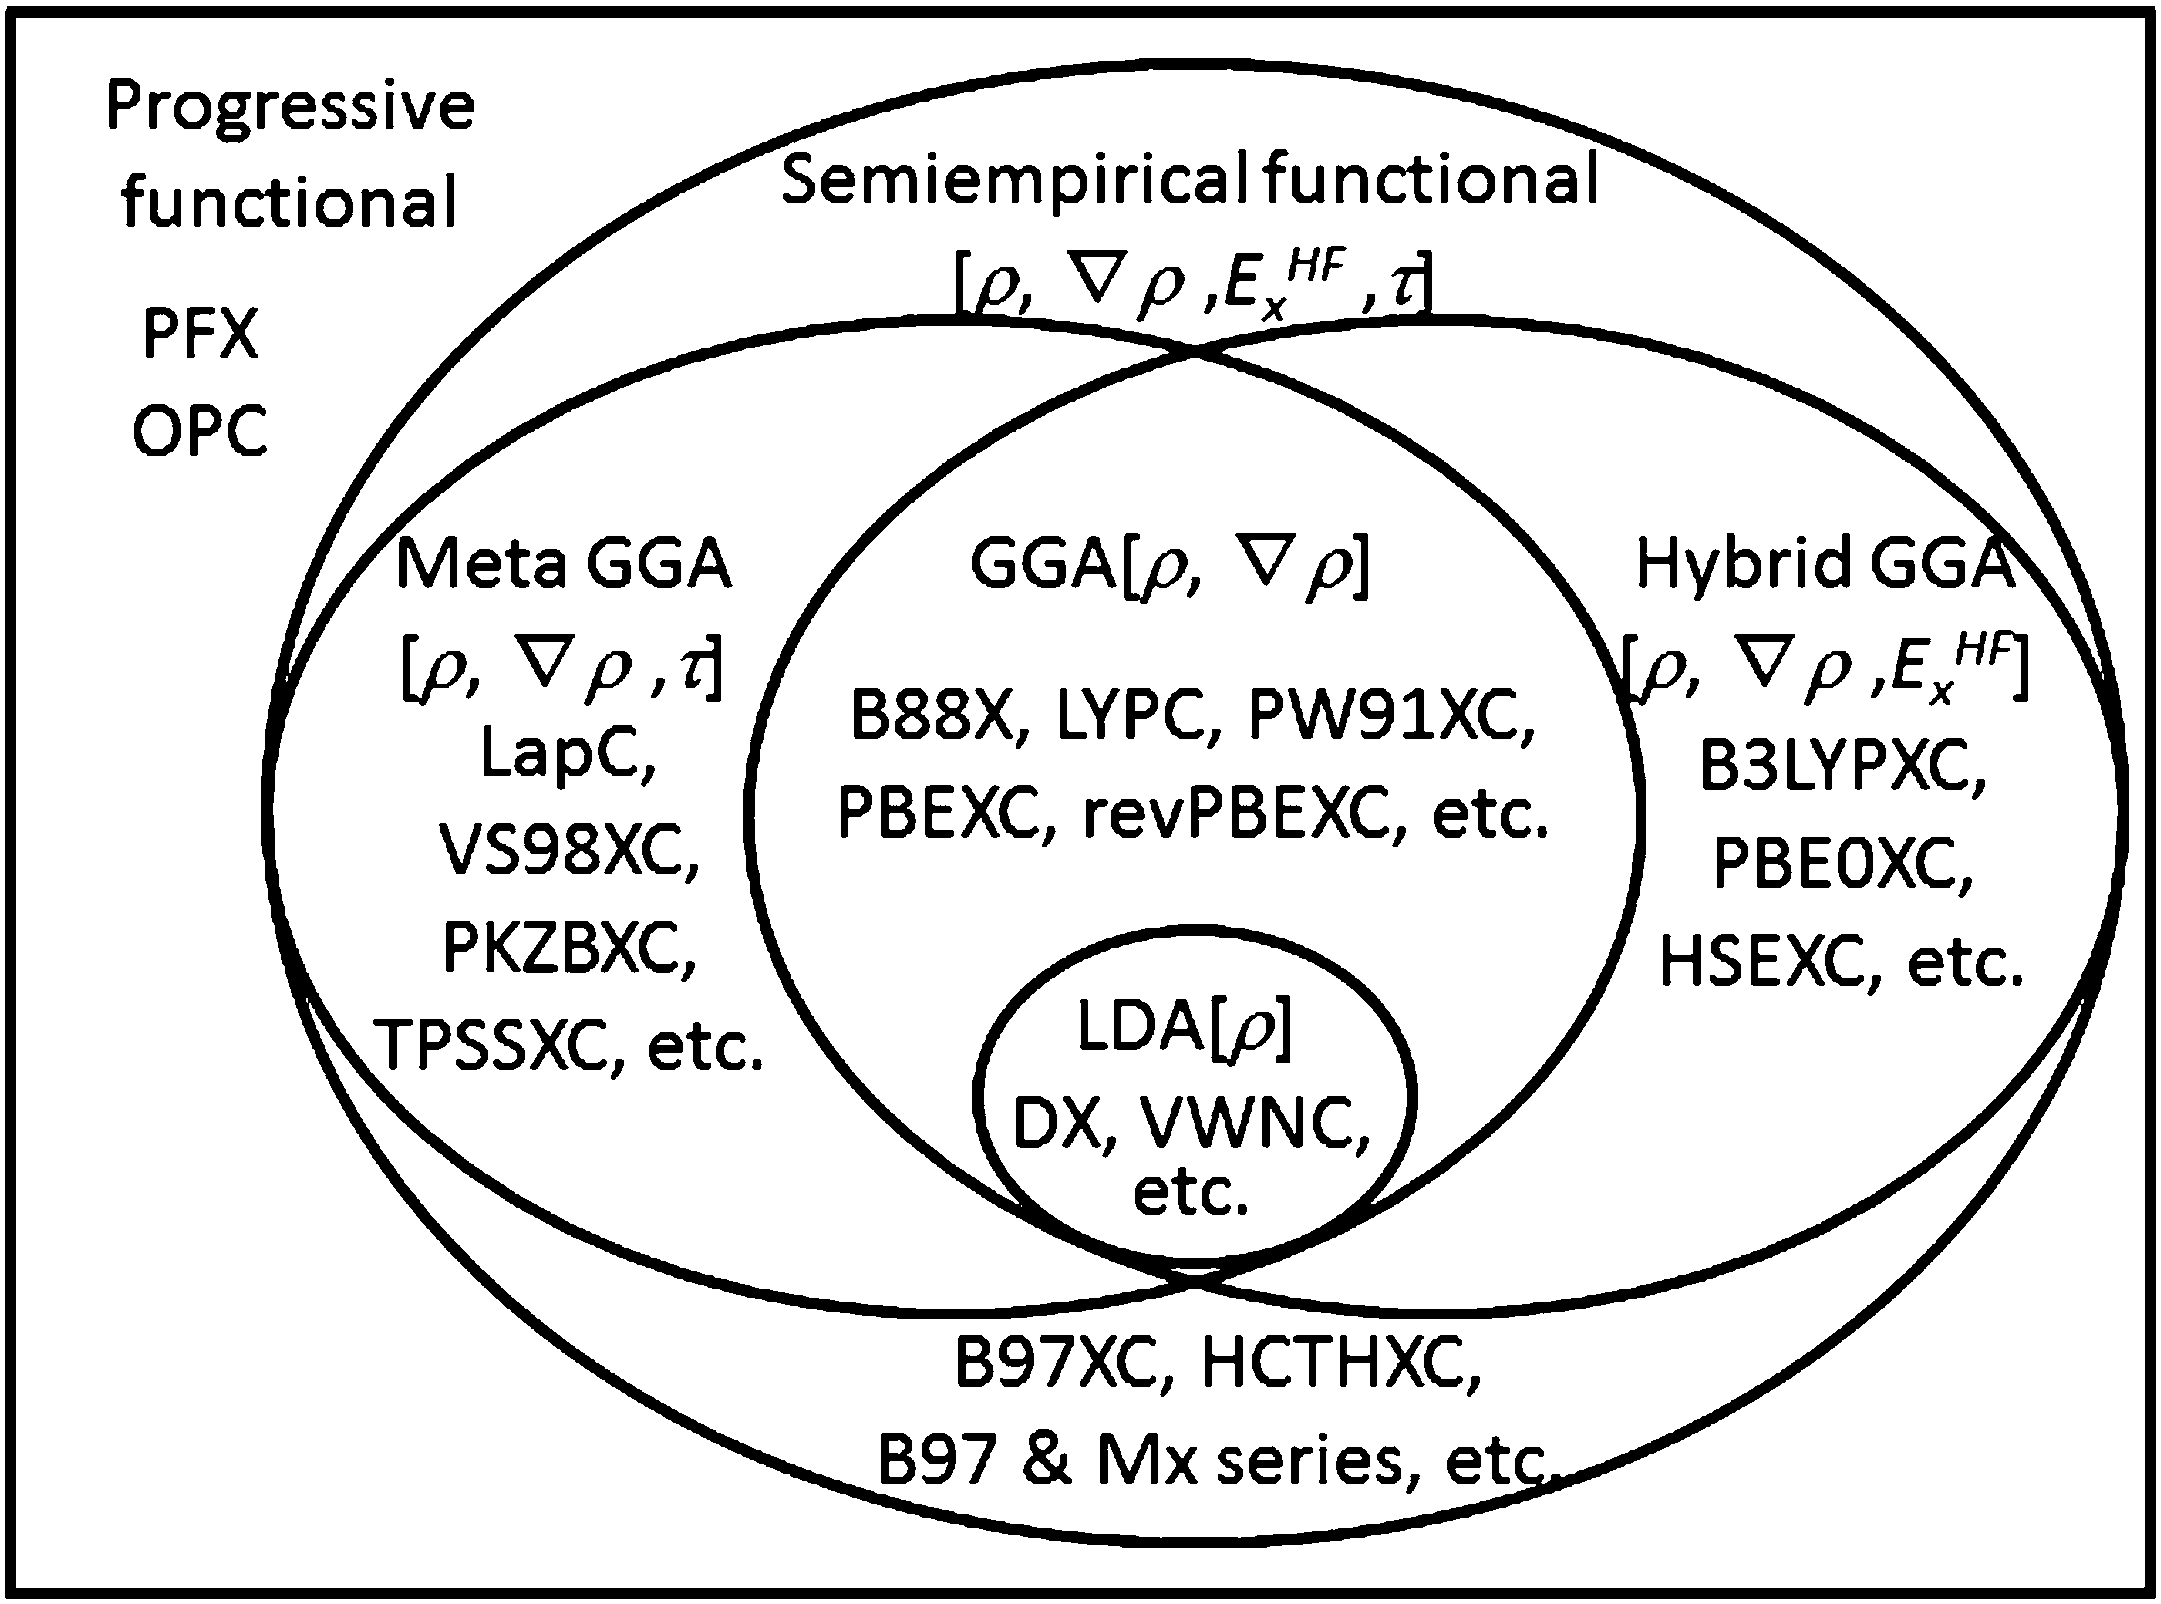
\includegraphics[width=0.5\textwidth]{functional-classification.png}
    \caption{交换-关联泛函的分类}
    \label{fig:excahnge-correlation-functional}
\end{figure}

\subsection{LDA近似}

当电子密度变化非常平缓时,$\grad{\rho},\laplacian{\rho}$等全部可以看成是零,此时交换关联泛函的形式是
\begin{equation}
    E_\text{XC}[\rho(\vb*{r})] = \int \dd[3]{\vb*{r}} \rho(\vb*{r}) \epsilon_\text{XC}(\rho(\vb*{r})).
\end{equation}
这就是所谓的局域密度近似:每单位的交换关联能只和该地点的电子密度有关。

首先我们尝试找一个适用于均匀自由电子气的交换关联泛函。我们取它为均匀自由电子气的基态的交换能加关联能就可以,即
\begin{equation}
    E_\text{XC}[\rho] = E_\text{X}[\rho] + E_\text{C}[\rho].
\end{equation}
自由电子气的基态就是费米面以内的每个轨道都占据了一上一下两个电子的状态,我们设共有$N$个电子,那么这些电子占据了$N/2$个不同的轨道。设这些轨道为$\{\phi_i(\vb*{r})\}$。
仅考虑库伦相互作用引入的一阶微扰,则有
\[
    E = \sum_{\sigma, \sigma'} \mel{\Psi}{
        \frac{1}{2} \int \dd[3]{\vb*{r}} \dd[3]{\vb*{r}'} {\psi}^\dagger_{\sigma}(\vb*{r}) {\psi}^\dagger_{\sigma'}(\vb*{r}') \frac{1}{\abs{\vb*{r} - \vb*{r}'}} {\psi}_{\sigma'}(\vb*{r}') {\psi}_\sigma(\vb*{r})
    }{\Psi}.
\]
这里必须完整地考虑自旋自由度的作用。可以使用Wick定理把上式展开,从而得到Hartree-Fock近似型的表达式。
请注意由于均匀电子气中没有自旋翻转,任何形如
\[
    \mel{\Psi}{{\psi}_\sigma^\dagger {\psi}_{\sigma'}}{\Psi}, \quad \sigma \neq \sigma'
\]
的项都是零,而
\[
    \mel{\Psi}{{\psi}^\dagger_\sigma(\vb*{r}) {\psi}_{\sigma}(\vb*{r}')}{\Psi} = \sum_i \phi_i^*(\vb*{r}) \phi_i(\vb*{r}'),
\]
于是最后能量修正为
\[
    E = \frac{1}{2} \int \dd[3]{\vb*{r}} \dd[3]{\vb*{r}'} \frac{1}{\abs{\vb*{r} - \vb*{r}'}} \bigg(
        \underbrace{4 \sum_{i} \abs{\phi_i(\vb*{r})}^2 \sum_{i} \abs{\phi_i(\vb*{r}')}^2}_\text{classical coulomb energy} - \underbrace{2 \sum_i \phi_i^*(\vb*{r}) \phi_i(\vb*{r}') \sum_i \phi_i^*(\vb*{r}') \phi_i(\vb*{r})}_\text{exchange energy}
    \bigg).
\]
交换能项前面的因子是$2$而不是$4$是因为自旋不同的电子之间的交换能全部抵消了。这样交换能就是
\begin{equation}
    E_\text{X} = - \int \dd[3]{\vb*{r}} \dd[3]{\vb*{r}'} \frac{1}{\abs{\vb*{r} - \vb*{r}'}} \abs{\sum_i \phi_i^*(\vb*{r}) \phi_i(\vb*{r}')}^2 . 
    \label{eq:exchange-energy-homogeneous-gas}
\end{equation}
对箱归一化的均匀电子气,有
\[
    \phi_i(\vb*{r}) = \frac{1}{\sqrt{V}} \ee^{- \ii \vb*{k}_i \cdot \vb*{r}},
\]
于是就有
\begin{equation}
    \sum_i \phi_i^*(\vb*{r}) \phi_i(\vb*{r}') = \sum_{\text{occupied $\vb*{k}$}} \frac{1}{V} \ee^{\ii \vb*{k} \cdot (\vb*{r} - \vb*{r}')} = \frac{1}{(2\pi)^3} \int_{\abs{\vb*{k}} < k_\text{F}} \dd[3]{\vb*{k}} \ee^{\ii \vb*{k} \cdot (\vb*{r} - \vb*{r}')},
    \label{eq:homogeneous-density}
\end{equation}
特别的,电子密度的一半(因为只考虑了轨道自由度)为
\[
    n(\vb*{r}) / 2 = \frac{k_\text{F}^3}{6 \pi^2}.
\]
上式代入\eqref{eq:exchange-energy-homogeneous-gas}就得到交换能的形式。
在这里我们稍微做一些推广。考虑一个非均匀的自由电子气,其非均匀性可能来自一些杂质或者特殊的相互作用,总之,每一个宏观小微观大的体积元可以看成一个用于归一化波函数的箱子,波函数定域在这个箱子里面(杂质会导致局域化)。
这样只有$\vb*{r} - \vb*{r}'$不超出一个箱子时\eqref{eq:homogeneous-density}才有明显的非零值。
每个箱子都有自己的费米动量,记作$k_\text{F}(\vb*{r})$(具体是关于$\vb*{r}$还是$\vb*{r}'$无关紧要因为两者总是在同一个箱子内)。
令
\[
    \vb*{s} = \vb*{r} - \vb*{r}', 
\]
则
\[
    \begin{aligned}
        E_\text{X} &= - \int \dd[3]{\vb*{r}} \dd[3]{\vb*{s}} \frac{1}{s} \left( \frac{1}{(2\pi)^3} \int_{\abs{\vb*{k}} < k_\text{F}} \dd[3]{\vb*{k}} \ee^{\ii \vb*{k} \cdot \vb*{s}} \right)^2 \\
        &= - \int \dd[3]{\vb*{r}} \dd[3]{\vb*{s}} \frac{1}{s} \left( \frac{3}{2} \frac{\sin t - t \cos t}{t^3} n(\vb*{r}) \right)^2 \quad (t= k_\text{F}(\vb*{r}) s) \\
        &= - 9 \pi \int \dd[3]{\vb*{r}} \int \dd{t} \frac{t}{k_\text{F}(\vb*{r})^2} n(\vb*{r})^2 \left( \frac{\sin t - t \cos t}{t^3} \right)^2 \\
        &= - \frac{3}{4} \left( \frac{3}{\pi} \right)^{1/3} \int \dd[3]{\vb*{r}} \rho(\vb*{r})^{4/3}.
    \end{aligned}
\]
这就得到了\concept{托马斯-费米-狄拉克泛函}:
\begin{equation}
    E_\text{X}[\rho] = - \frac{3}{4} \left( \frac{3}{\pi} \right)^{1/3} \int \dd[3]{\vb*{r}} \rho(\vb*{r})^{4/3} = - 0.7386 \int \dd[3]{\vb*{r}} \rho(\vb*{r})^{4/3}
\end{equation}
对均匀或不均匀但缓变的电子气这个泛函适用。

\subsection{GGA近似}

\section{Kohn-Sham方程的求解}

\autoref{alg:basic-kohn-sham}给出的只是求解\eqref{eq:kohn-sham-eq}的方法,而实际的凝聚态计算还需要考虑原子核的位置、携带的电荷(从而确定材料中的电子总量)等信息,即需要适当地将$V_\text{ext}$和$\mu$引入;此外\eqref{eq:kohn-sham-eq}本身是微分方程,求解它需要做适当的离散化,例如,我们可以将$\phi_i(\vb*{r})$函数在适当的基底(量子化学中通常称为\concept{基组})下展开。
本节给出几种常见的DFT计算任务。

\subsection{基于超胞的平面波DFT计算}\label{sec:supercell-pwdft}

\eqref{eq:kohn-sham-eq}中涉及的单电子波函数的个数要和系统中电子的数目一样多,否则$\rho(\vb*{r})$的总量不正确。
介质中的电子数目是非常多的,从而直接求解\eqref{eq:kohn-sham-eq}并不现实。
晶体有周期性结构,这就大大简化了计算。实际上,由于相互作用衰减得很快,我们完全可以假定液体等也有周期性边界条件,只不过此时的晶胞要取得非常大。

于是以下我们将DFT计算中被认为是周期性的单元称为\concept{超胞(supercell)},对固体通常要求超胞取最简单的形式,即原胞,对单分子、液体或是有杂质的系统等则需要取一个较大的超胞。
对杂质,超胞应该包括杂质周围足够大的体态。
对单分子,当超胞足够大时第一布里渊区足够小,从而计算出的所谓“能带”实际上和单独的一个个能级毫无区别。
我们需要指定超胞的几何形状,并且在超胞内给出各个原子核的位置。

由于\eqref{eq:kohn-sham-eq}此时就是周期性的,它的解——也就是$\phi_i(\vb*{r})$——可以看成某个以我们设定的超胞为原胞的晶体中的单电子波函数,从而Bloch定理\eqref{eq:bloch-wavefunction}成立,且$\phi_i(\vb*{r})$中的$i$应该替换成Bloch波矢$\vb*{k}$和能带标记$n$。
由于\eqref{eq:bloch-wavefunction}中的$u(\vb*{r})$具有周期性,它可以被展开成用倒格矢标记的一系列傅里叶分量,因此我们有
\begin{equation}
    \phi_{n \vb*{k}}(\vb*{r}) = \sum_{\vb*{G}} c_{n, \vb*{k}, \vb*{G}} \ee^{\ii (\vb*{k} + \vb*{G}) \cdot \vb*{r}},
\end{equation}
或者,考虑到$\vb*{k}$局限在第一布里渊区中而$\vb*{G}$是倒格矢,从$\vb*{k} + \vb*{G}$可以唯一确定$\vb*{k}$和$\vb*{G}$,有
\begin{equation}
    \phi_{n \vb*{k}}(\vb*{r}) = \sum_{\vb*{G}} c_{n, \vb*{k} + \vb*{G}} \ee^{\ii (\vb*{k} + \vb*{G}) \cdot \vb*{r}}.
\end{equation}
这种选取$\phi_i$的方法称为\concept{平面波DFT(PWDFT)}。

上式的$\vb*{G}$分量在\eqref{eq:kohn-sham-eq}的动能项部分为$(\vb*{k} + \vb*{G})^2 / 2m$,由于实际能够存储的傅里叶分量的个数是有限的,通常会引入一个\concept{截断能},对每个$\vb*{k}$,我们只保留对动能的贡献小于截断能的那些$\vb*{G}$。
这意味着我们忽略了空间尺度特别小的现象,并且忽略了一部分能量,但是如果对应的$c_{n, \vb*{k} + \vb*{G}}$不大就没有什么问题。

实际能够处理的晶体都是有限大小的,或者说实际的$\vb*{k}$的取值是第一布里渊区中离散的一些点。
这就是说,我们需要给出一种“第一布里渊区中的动量采样”。
显然,采样越密越好;可以使用$\vb*{k} \cdot \vb*{p}$来简化计算。

最后我们处理至今尚未提及的$V_\text{ext}$。如\autoref{sec:pseudopotential}所述,外层电子感受到的势场可以用赝势取代。
这里我们有好几种可能的做法:可以只计算外层电子,完全不计算内层电子,从而自始至终$V_\text{ext}$都是用赝势组合而成的。此时截断能可以设置得比较小,因为$\phi_{n \vb*{k}}(\vb*{r})$在靠近原子核的位置也不会发生剧烈振荡。
也可以用赝势计算出初步的电子密度,然后改用库伦势做进一步计算。

\begin{algorithm}

    \DontPrintSemicolon
    \SetAlgoLined

    \KwData{初始电子密度$\rho_0(\vb*{r})$,交换关联泛函选取$E_\text{XC}[\rho(\vb*{r})]$,不同原子的赝势,$\vb*{k}$点采样$K = \{\vb*{k}\}$,截断能$E_\text{cut}$,最大迭代次数$N_\text{max}$,容差$\epsilon$}
    \KwResult{Kohn-Sham波函数$\phi_{n \vb*{k}}(\vb*{r})$和对应的本征值$\epsilon_{n \vb*{k}}$}
    
    \For{$\vb*{k} \in K$}{
        根据$\frac{(\vb*{k} + \vb*{G})^2}{2m} < E_\text{cut}$确定 \;
    } % TODO:

    $i = 1$ \;
    使用不同原子的赝势构造\eqref{eq:kohn-sham-eq}中的$V_\text{ext}$ \;
    将$\rho_0(\vb*{r})$代入\eqref{eq:kohn-sham-eq}求解得到$\phi_n^{(1)}$和$\epsilon_n^{(1)}$ \;
    将$\phi_n^{(1)}$代入\eqref{eq:kohn-sham-density}计算得到$\rho_1(\vb*{r})$ \;
    \While{$\rho_i(\vb*{r})$和$\rho_{i-1}(\vb*{r})$的差别大于容差$\epsilon$且$i < N_\text{max}$}{
        将$\rho_i$代入\eqref{eq:kohn-sham-eq}求解得到$\phi_n^{(i+1)}$和$\epsilon_n^{(i+1)}$ \;
        $i = i + 1$ \;
    }
    
    \Return{波函数$\phi^{(i)}_n$和本征值$\epsilon^{(i)}_n$}\;

    \caption{给定晶格和原子赝势的PWDFT计算}
    \label{alg:static-pwdft}
\end{algorithm}

将以上考虑放进\autoref{alg:basic-kohn-sham}中,我们得到\autoref{alg:static-pwdft},即所谓\concept{静态自洽计算}。
只要输入的晶体结构是准确的,交换关联泛函的质量足够好,我们就得到了外层电子或是全电子(一般来说用不到,因为化学反应的能级不足以激发内层电子,倒是从头计算赝势时需要全电子计算)的模拟结果:这其中没有引入任何经验参数,并且每一条可能的能带都纳入了考虑。
虽然如此,截断能、$\vb*{k}$点采样、赝势的选择仍然会显著影响计算精度。

有时候我们对晶体结构只有一个大概的猜测,此时需要做结构优化,即所谓\concept{结构优化自洽计算}。

\begin{info}{VASP软件包}{vasp}
    在
\end{info}

% TODO:类似于确定每一条带上的电子磁矩如何,电荷密度等等

\section{低温下的电子配对}\label{sec:low-and-super}

很多集体行为和相变均可以通过经典的金斯堡-朗道理论加以描述:相变的出现是因为某个对称性被破缺了,然后我们可以使用某个序参量来描述相变,而序参量的涨落就给出了相变之后产生的元激发。
我们可以使用Hubbard-Stratonovich变换将二体相互作用解耦,适当选取Hubbard-Stratonovich参量使之和序参量对应,然后积掉电子自由度和声子自由度,这样就得到了元激发的有效理论。
序参量应该是通常是一些电子场算符的乘积或其线性组合,元激发是序参量的涨落,即元激发实际上是多个电子(或者也许还有声子或其他粒子)的集体行为,或者说\concept{粒子凝聚}。

费米子体系中可以有各种各样的这种电子凝聚:自旋密度波%
\footnote{
    为了避免引起混淆我们要区分自旋密度波和自旋波。后者是一个自旋系统中的现象,前者是一个费米子系统中的现象。
    或者,更加形象地说,后者是固定在格点上的自旋的空间涨落,前者是可以运动的、携带自旋的费米子密度的空间涨落。
}%
、电荷密度波、超导配对等。电子配对顾名思义,可能导致可以不受阻碍地随意移动的“超导电子”出现;所谓密度波实际上就是一种长程序,它在空间中有一种周期性振荡,可以是相位的振荡也可以是大小的振荡,
也即,这样的长程序对应的序参量形如%
\footnote{请注意这个序参量实际上是一种二电子集体运动模式,即相邻的两个电子的自旋总是保持一上一下的这种运动模式。
这暗示我们,如果需要超越平均场近似的理论,只需要把这种模式定义成一个新的(玻色)场就可以。
这个技巧和一维电子系统的玻色化很相似。}%
\begin{equation}
    \Delta(\vb*{r}) \sim \Delta_0 \ee^{\ii \vb*{Q} \cdot \vb*{r}}.
\end{equation}
这些现象对应的序参量对应于Hubbard-Stratonovich参量的不同选择;换句话说,不同的相互作用通道相互竞争,最终哪一种相互作用通道占据优势——从而,单单考虑它得到的相变出现——取决于很多条件。
% TODO:费米液体图像失效

应当指出的是这个图像并不能覆盖所有相变。例如在

\subsection{BCS超导}

本节介绍一种常见的超导机制,即交换声子导致电子出现有效吸引相互作用而产生的BCS超导。

\subsubsection{交换声子导致的有效电子吸引相互作用}\label{sec:phonon-caused-interaction}

电子-声子相互作用的顶角为一个电子入射,一个电子出射,产生/消灭一个声子。
现在尝试积掉声子。我们先将电子场当成给定的,则可以从\eqref{eq:simple-phonon-electron-int}写出声子场加上电子-声子相互作用的虚时间作用量。本节仅考虑晶格是简单正方晶格的情况,于是没有各向异性,我们有
\[
    S_\text{ph} + S_\text{int} = \sum_{\omega_n, \vb*{q}, \lambda} \Big(
        \bar{\phi}_{\vb*{q} \lambda} (- \ii \omega_n + \omega_q) \phi_{\vb*{q} \lambda}
        + \gamma \frac{\ii q_\lambda}{\sqrt{2 M \omega_q}} (\phi_{\vb*{q} \lambda} + \bar{\phi}_{-\vb*{q} \lambda}) \underbrace{\sum_{\vb*{k}, \sigma} \bar{\psi}_{(\vb*{k} + \vb*{q}) \sigma} \psi_{\vb*{k} \sigma}}_{\rho_{\vb*{q}}}
    \Big),
\]
其中$\phi$表示声子,$\psi$表示电子。使用处理自由场受到线性激励的方法,配平方并积掉二次方项,忽略产生的因子,得到
\begin{equation}
    \begin{aligned}
        S_\text{eff} &= - \sum_{\omega_n, \vb*{q}} \frac{\gamma^2 q^2 \rho_{\vb*{q}} \rho_{-\vb*{q}}}{2 M \omega_q (\omega_q - \ii \omega_n)} 
        = - \sum_{\omega_n, \vb*{q}} \frac{\gamma^2 q^2 \rho_{\vb*{q}} \rho_{-\vb*{q}}}{2 M (\omega_q^2 + \omega_n^2)} \\ 
        &= - \frac{\gamma^2}{2 M} \sum_{\omega_n} \sum_{\vb*{q}, \vb*{k}, \vb*{k}', \alpha, \beta} \frac{q^2}{\omega_n^2 + \omega_q^2} \bar{\psi}_{(\vb*{k}+\vb*{q}) \alpha} \bar{\psi}_{(\vb*{k}' - \vb*{q}) \beta} \psi_{\vb*{k}' \beta} \psi_{\vb*{k} \alpha} .
    \end{aligned}
    \label{eq:retarded-two-electron}
\end{equation}
第二个等号是考虑到每个$\omega_n$有一个对应的$-\omega_n$而得到的。总之,电子之间可以通过交换声子来产生一个四电子相互作用。
相互作用\eqref{eq:retarded-two-electron}是推迟相互作用,因此原则上不能够仅仅使用一个哈密顿量描述。
不过,在推迟不明显时我们还是可以近似写出一个哈密顿量。这里有一个微妙的地方:\eqref{eq:retarded-two-electron}是定义在虚时间下的,即算符的时间演化为$\ee^{\omega t}$,而我们需要一个实时间下的哈密顿量,所以需要首先做频率上的Wick转动$\omega = \ii \omega_n$,得到
\[
    S_\text{eff}^\text{real} = - \frac{\gamma^2}{2 M} \int \dd{\omega} \sum_{\vb*{q}, \vb*{k}, \vb*{k}', \alpha, \beta} \frac{q^2}{- \omega^2 + \omega_q^2} \bar{\psi}_{(\vb*{k}+\vb*{q}) \alpha} \bar{\psi}_{(\vb*{k}' - \vb*{q}) \beta} \psi_{\vb*{k}' \beta} \psi_{\vb*{k} \alpha}.
\]
上式中的所有$\psi$都是$\omega$的函数,可以将它们转换到时域;我们也知道,上式的无推迟近似是它的无时间变化的傅里叶分量。
因此实际上我们只需要简单地取
\begin{equation}
    \omega = \epsilon_{\vb*{k}} - \epsilon_{\vb*{k} + \vb*{q}},
    \label{eq:phonon-introduced-omega}
\end{equation}
就得到了无推迟的近似
\begin{equation}
    \begin{aligned}
        {H} &= - \frac{\gamma^2}{2 M} \sum_{\vb*{q}, \vb*{k}, \vb*{k}', \alpha, \beta} \frac{q^2}{- \omega^2 + \omega_q^2} {c}^\dagger_{(\vb*{k}+\vb*{q}) \alpha} {c}^\dagger_{(\vb*{k}' - \vb*{q}) \beta} {c}_{\vb*{k}' \beta} {c}_{\vb*{k} \alpha} \\
        &= \frac{\gamma^2}{2 M} \sum_{\vb*{q}, \vb*{k}, \vb*{k}', \alpha, \beta} \frac{q^2}{(\epsilon_{\vb*{k}} - \epsilon_{\vb*{k}+\vb*{q}})^2 - \omega_q^2} {c}^\dagger_{(\vb*{k}+\vb*{q}) \alpha} {c}^\dagger_{(\vb*{k}' - \vb*{q}) \beta} {c}_{\vb*{k}' \beta} {c}_{\vb*{k} \alpha}.
    \end{aligned}
\end{equation}

我们写出以下更加一般的哈密顿量:
\begin{equation}
    {H}_{4\text{e}} = \frac{1}{2N} \sum_{\vb*{k}, \vb*{k}', \vb*{q}'} \sum_{\alpha, \beta} \abs{M_{\vb*{q}}}^2 \frac{\omega_{\vb*{q}}}{(\epsilon_{\vb*{k}} - \epsilon_{\vb*{k}+\vb*{q}})^2 - \omega_{\vb*{q}}^2} {c}^\dagger_{(\vb*{k}+\vb*{q}) \alpha} {c}^\dagger_{(\vb*{k}'-\vb*{q}) \beta} {c}_{\vb*{k}' \beta} {c}_{\vb*{k} \alpha},
    \label{eq:4-electron-interaction-by-phonon}
\end{equation}
其中$\omega_{\vb*{q}}$表示声子能量。任何更复杂的含有声子的费曼图都可以化归为二电子和声子的相互作用和一些电子相互作用的组合,因此\eqref{eq:4-electron-interaction-by-phonon}就给出了完整的没有声子的有效理论。
\eqref{eq:4-electron-interaction-by-phonon}本身是瞬时的,但即使我们不知道它来自一个推迟相互作用,\eqref{eq:4-electron-interaction-by-phonon}含有电子能量差而\eqref{eq:phonon-introduced-omega}也有这一事实也暗示它有可能实际上代表一个推迟相互作用。
另一方面,库伦势则没有推迟(当然这实际上做了近似,我们只不过不考虑相对论效应而已,但是电磁相互作用的推迟远小于声子传递导致的推迟)。

现在考虑一个低能有效理论%
\footnote{这就是超导往往发生在低温下的原因:否则没法形成电子的有效吸引,四散排斥的电子会造成很大耗散。}%
,其中我们需要考虑的过程全部发生在费米面附近,入射电子和出射电子能量都接近于$\epsilon_\text{F}$。
费米面是球形的,通过几何关系可以看出$\vb*{k} + \vb*{k}' = 0$的过程是最重要的,此时发生相互作用前两个电子始终在费米面的两端,相互作用之后两个电子还是位于费米面的两端。
这样\eqref{eq:4-electron-interaction-by-phonon}就简化为
\begin{equation}
    {H}_{4\text{e}} = \frac{1}{2N} \sum_{\vb*{k}, \vb*{q}'} \underbrace{\sum_{\alpha, \beta} \abs{M_{\vb*{q}}}^2 \frac{\omega_{\vb*{q}}}{(\epsilon_{\vb*{k}} - \epsilon_{\vb*{k}+\vb*{q}})^2 - \omega_{\vb*{q}}^2}}_{V(\vb*{q}, \epsilon_{\vb*{k}} - \epsilon_{\vb*{k}+\vb*{q}})} {c}^\dagger_{(\vb*{k}+\vb*{q}) \alpha} {c}^\dagger_{(-\vb*{k}-\vb*{q}) \beta} {c}_{-\vb*{k} \beta} {c}_{\vb*{k} \alpha}.
    \label{eq:low-energy-4-electron}
\end{equation}
由于电子能量差非常小,显然
\[
    V(\vb*{q}, \epsilon_{\vb*{k}} - \epsilon_{\vb*{k}+\vb*{q}}) = \abs{M_{\vb*{q}}}^2 \frac{\omega_{\vb*{q}}}{(\epsilon_{\vb*{k}} - \epsilon_{\vb*{k}+\vb*{q}})^2 - \omega_{\vb*{q}}^2} < 0,
\]
因此这个声子中介的相互作用是吸引相互作用。

库伦相互作用是排斥的,电-声子相互作用是吸引的;绝对强度显然是前者强。
然而,实际上库伦相互作用很容易被屏蔽,因为把低能电子看成外加电荷,那么高能电子就会来屏蔽它(见\autoref{sec:ext-e}),因此把高能电子积掉之后得到的屏蔽库仑相互作用并不强,因此在重整化下,库仑相互作用实际上只是对电子能带的修正(这和费米液体的想法很相似:渐染地加入一个不大的相互作用仅仅会导致电子自能修正而已)。
另一方面,电-声子相互作用是不容易屏蔽的,实际上推迟相互作用就是不容易屏蔽的。
因此,\eqref{eq:low-energy-4-electron}在重整化之后是主要的电子间相互作用。
还有一种看待这个问题的方式是,电-声子相互作用会导致有效的吸引,在重整化下一个吸引相互作用通常会导致粒子配对取代单粒子自由度成为主要的自由度,因此吸引相互作用不可能只是对能带的修正;库仑相互作用在这里是排斥的,不会造成粒子配对,因此正如Hartree-Fock近似中的那样,仅仅对电子能级产生了一个修正。

声子的频率只出现在0和德拜频率$\omega_\text{D}$之间,换而言之吸引相互作用只出现在
\[
    \omega = \abs{\epsilon_{\vb*{k}} - \epsilon_{\vb*{k}+\vb*{q}}} < \omega_\text{D}
\]
时。数值计算可以表明对超导现象而言最重要的是建立起电子之间的吸引相互作用,其具体形式并不重要,这是因为会参与超导的实际上只有费米面附近的非常小的一个能量范围内的电子,因此$V$的具体形式根本不重要,实际发挥作用的只有费米面上的$V$值。
这样我们设
\begin{equation}
    V(\vb*{q}, \omega) = \begin{cases}
        - V_0, \quad \omega < \omega_\text{D}, \\
        0, \quad \omega > \omega_\text{D}
    \end{cases}.
    \label{eq:superconductive-interaction-simplified}
\end{equation}
其中$\omega_\text{D}$是一个硬截断。这是一个非常粗糙的截断,但后面会发现它是合理的。
这样整个系统的哈密顿量就是
\begin{equation}
    {H} = \sum_{\vb*{k}, \alpha} (\epsilon_{\vb*{k}} - \mu) {c}_{\vb*{k} \alpha}^\dagger {c}_{\vb*{k} \alpha} - \frac{V_0}{2} \sum_{\vb*{k}, \vb*{q}} \sum_{\alpha, \beta} {c}^\dagger_{(\vb*{k} + \vb*{q}) \alpha} {c}^\dagger_{( - \vb*{k} - \vb*{q}) \beta} {c}_{-\vb*{k} \beta} {c}_{\vb*{k} \alpha}.
    \label{eq:simple-super-conductive-hamiltonian}
\end{equation}
$\vb*{k}$和$\vb*{k}+\vb*{q}$都在费米面附近。

\subsubsection{库伯对}

数值计算或者手算二体问题会发现可能出现\concept{库伯对},即一对位于费米面上的电子配对。
这种配对写成算符形式就是${c}^\dagger {c}^\dagger$的形式,或者等价的${c} {c}$形式。
如果其期望值不为零,那么$U(1)$对称性就破缺了,即电荷守恒对称性被破缺了(物理图像是,一部分电荷被封存到了库伯对中,不再以独立电子的形式流动)。我们会看到电荷守恒的破缺实际上是低温超导中最重要的物理。
于是,库伯对序参量的一般形式显然是$\expval*{{c}_{\vb*{k}\alpha} {c}_{\vb*{k}' \beta}}$。

现在我们做对称性分析。注意到时间反演对称性要求
\[
    \epsilon_{\vb*{k} \uparrow} = \epsilon_{-\vb*{k} \downarrow},
\]
而\eqref{eq:simple-super-conductive-hamiltonian}中单电子能量和自旋无关,于是
\[
    \epsilon_{\vb*{k}} = \epsilon_{-\vb*{k}}.
\]
这样就容易验证\eqref{eq:simple-super-conductive-hamiltonian}在变换$\vb*{k} \longrightarrow -\vb*{k}$下不变,这个对称性没有被破缺掉,于是
\[
    \expval*{{c}_{\vb*{k}\alpha} {c}_{\vb*{k}' \beta}} \propto \delta(\vb*{k} + \vb*{k}').
\]
换而言之,我们只考虑总动量为零的配对$\expval*{{c}_{\vb*{k} \alpha} {c}_{- \vb*{k} \beta}}$。
此外还可以发现\eqref{eq:simple-super-conductive-hamiltonian}具有自旋旋转不变性,因此相应的序参量$\expval*{{c}_{\vb*{k} \alpha} {c}_{- \vb*{k} \beta}}$应该是一个二分量的自旋协变的对象。二粒子配对对应的$SU(2)$的表示为
\[
    \frac{1}{2} \otimes \frac{1}{2} = 0 \oplus 1,
\]
即可能有自旋单态也可能有自旋三重态。如果该库伯对是自旋单态,那么应该有
\[
    \expval*{{c}_{\vb*{k} \alpha} {c}_{- \vb*{k} \beta}} \propto \epsilon_{\alpha \beta} \propto \delta_{\alpha+\beta,0},
\]
其中$\epsilon$为所谓的旋量度规;而如果该库珀对为自旋三重态,那么就应该有
\[
    \expval*{{c}_{\vb*{k} \alpha} {c}_{- \vb*{k} \beta}} \propto \vb*{d} \cdot \vb*{\sigma}_{\alpha \beta}.
\]
% TODO:为什么??
最后,由于没有自旋-轨道耦合,$\expval*{{c}_{\vb*{k} \alpha} {c}_{- \vb*{k} \beta}}$可以写成“动量部分乘以自旋部分”的形式。
这样我们设
\[
    \expval*{{c}_{\vb*{k} \alpha} {c}_{- \vb*{k} \beta}} \propto \Delta(\vb*{k}).
\]
如果该库伯对是自旋单态的,那么其自旋部分是反对称的,则其轨道部分就是对称的,也即
\[
    \Delta(\vb*{k}) = \Delta(-\vb*{k}),
\]
从而可以将$\Delta(\vb*{k})$展开成一系列s波、d波等对称球谐函数的线性组合;
而如果该库伯对是自旋三重态的,那么其自旋部分就是对称的,于是轨道部分满足
\[
    \Delta(\vb*{k}) = -\Delta(-\vb*{k}),
\]
此时$\Delta(\vb*{k})$是一系列反对称球谐函数的线性组合。
容易看出单态或者三重态的出现和费米面对称性的关系,比如如果费米面不对称,那么s波配对就不能产生。

\subsubsection{平均场近似和Bogoliubov变换}

对\eqref{eq:simple-super-conductive-hamiltonian}做平均场近似,有
\[
    \begin{aligned}
        & \quad {c}^\dagger_{(\vb*{k} + \vb*{q}) \alpha} {c}^\dagger_{( - \vb*{k} - \vb*{q}) \beta} {c}_{-\vb*{k} \beta} {c}_{\vb*{k} \alpha} \\
        &\approx \expval*{{c}^\dagger_{(\vb*{k} + \vb*{q}) \alpha} {c}^\dagger_{( - \vb*{k} - \vb*{q}) \beta}} {c}_{-\vb*{k} \beta} {c}_{\vb*{k} \alpha} + {c}^\dagger_{(\vb*{k} + \vb*{q}) \alpha} {c}^\dagger_{( - \vb*{k} - \vb*{q}) \beta} \expval*{{c}_{-\vb*{k} \beta} {c}_{\vb*{k} \alpha}} - \expval*{{c}^\dagger_{(\vb*{k} + \vb*{q}) \alpha} {c}^\dagger_{( - \vb*{k} - \vb*{q}) \beta} {c}_{-\vb*{k} \beta} {c}_{\vb*{k} \alpha}},
    \end{aligned}
\]
重新选定求和哑指标,并略去对体系动力学没有影响的常数项,得到
\begin{equation}
    {H}_\text{MF} = \sum_{\vb*{k}, \alpha} (\epsilon_{\vb*{k}} - \mu) {c}_{\vb*{k} \alpha}^\dagger {c}_{\vb*{k} \alpha} - \frac{V_0}{2} \sum_{\vb*{k}, \vb*{k}', \alpha, \beta} \left(
        \expval*{{c}_{-\vb*{k} \beta} {c}_{\vb*{k} \alpha}} {c}^\dagger_{\vb*{k}' \alpha} {c}^\dagger_{- \vb*{k}' \beta} + \text{h.c.} 
    \right).
\end{equation}
的确,电荷守恒对称性被破缺了,原因是电子形成库伯对之后看起来就像被“冻结”了一样,因此不再被计入${c}^\dagger$自由度中,而是被计入序参量$\expval*{{c}_{-\vb*{k} \beta} {c}_{\vb*{k} \alpha}}$中。

现在我们考虑单态、s波的库伯对,这样发生配对的就是一个$\vb*{k}, \uparrow$态的电子和一个$-\vb*{k}, \downarrow$态的电子,或者做一个自旋旋转。总之,序参量可以选取为
\begin{equation}
    \Delta = - \frac{V_0}{2} \sum_{\vb*{k}} (
        \expval*{{c}_{-\vb*{k}\uparrow} {c}_{\vb*{k} \downarrow}} - \expval*{{c}_{-\vb*{k} \downarrow} {c}_{\vb*{k} \uparrow}}
    ) = -V_0 \sum_{\vb*{k}} \expval*{{c}_{-\vb*{k}\uparrow} {c}_{\vb*{k} \downarrow}} ,
    \label{eq:superconductive-order-parameter}
\end{equation}
则可以证明
\begin{equation}
    {H}_\text{MF} = \sum_{\vb*{k}, \alpha} \xi_{\vb*{k}} {c}_{\vb*{k} \alpha}^\dagger {c}_{\vb*{k} \alpha} 
    + \Delta \sum_{\vb*{k}} {c}_{-\vb*{k} \downarrow}^\dagger {c}^\dagger_{\vb*{k} \uparrow}
    + \Delta^* \sum_{\vb*{k}} {c}_{\vb*{k} \uparrow} {c}_{-\vb*{k} \downarrow}.
    \label{eq:s-wave-superconductive-hamiltonian}
\end{equation}

在\eqref{eq:s-wave-superconductive-hamiltonian}中总是可以对${c}$和${c}^\dagger$做一个幺正变换,让$\Delta$为实数,因此以下假定$\Delta$为实数。
用一个幺正变换重新定义一组准粒子(这就称为\concept{Bogoliubov变换}),使这组准粒子本身是费米子,并且能够让\eqref{eq:s-wave-superconductive-hamiltonian}对角化(从而这组准粒子的能谱就是\eqref{eq:s-wave-energy-band})。
首先我们有费米子的对易关系
\[
    \acomm*{{\gamma}_{\vb*{k}_1 \alpha}}{{\gamma}^\dagger_{\vb*{k}_2 \beta}} = \delta_{\vb*{k}_1 \vb*{k}_2} \delta_{\alpha \beta}, \quad \acomm*{{\gamma}_{\vb*{k}_1 \alpha}}{{\gamma}_{\vb*{k}_2 \beta}} = 0,
\]
并且可以看到,以下正交变换
\[
    \pmqty{{\gamma}_{\vb*{k} \uparrow} \\ {\gamma}^\dagger_{-\vb*{k} \downarrow}} = \pmqty{u_{\vb*{k}} & -v_{\vb*{k}} \\ v_{\vb*{k}} & u_{\vb*{k}}} \pmqty{{c}_{\vb*{k} \uparrow} \\ {c}^\dagger_{-\vb*{k} \downarrow}},
    \quad u_{\vb*{k}}^2 + v_{\vb*{k}}^2 = 1
\]
能够给出正确的对易关系,则可以解出
\begin{equation}
    u_{\vb*{k}} = \sqrt{\frac{E_{\vb*{k}} + \xi_{\vb*{k}}}{2 E_{\vb*{k}}}}, \quad v_{\vb*{k}} = \sqrt{\frac{E_{\vb*{k}} - \xi_{\vb*{k}}}{2 E_{\vb*{k}}}}.
\end{equation}
这就得到了Bogoliubov变换的显式形式:
\begin{equation}
    \begin{cases}
        {\gamma}_{\vb*{k} \uparrow} = u_{\vb*{k}} {c}_{\vb*{k} \uparrow} - v_{\vb*{k}} {c}_{-\vb*{k} \downarrow}^\dagger, \\
        {\gamma}_{\vb*{k} \downarrow} = u_{\vb*{k}} {c}_{\vb*{k} \downarrow} + v_{\vb*{k}} {c}_{-\vb*{k} \uparrow}^\dagger,
    \end{cases}
    \label{eq:bogoliubov-transform}
\end{equation}
还有它的逆变换
\begin{equation}
    \begin{cases}
        {c}_{\vb*{k} \uparrow} = u_{\vb*{k}} {\gamma}_{\vb*{k} \uparrow} + v_{\vb*{k}} {\gamma}_{-\vb*{k} \downarrow}^\dagger, \\
        {c}_{\vb*{k} \downarrow} = u_{\vb*{k}} {\gamma}_{\vb*{k} \downarrow} - v_{\vb*{k}} {\gamma}_{-\vb*{k} \uparrow}^\dagger.
    \end{cases}
    \label{eq:inverse-bogoliubov-transform}
\end{equation}
由于从${c}$到${\gamma}$的线性变换是一个正交变换%
\footnote{这件事不是一般成立的,有时候真的要用一个非正交变换;关键在于对易关系必须正确,不是所有的线性变换形式都能够给出正确的对易关系。}%
,\eqref{eq:s-wave-superconductive-hamiltonian}的能谱可以通过对角化矩阵的方式求出。
求解之后会发现能带为
\begin{equation}
    E_{\vb*{k}} = \pm \sqrt{ \xi_{\vb*{k}}^2 + \abs{\Delta}^2 }.
    \label{eq:s-wave-energy-band}
\end{equation}
这个结果具有粒子-空穴对称性,但是这并不具有太多物理意义,因为它实际上是对角化时交换了一对产生湮灭算符,从而把一部分粒子自由度写成了空穴而已。
\eqref{eq:s-wave-energy-band}中,序参量$\Delta$把原本发生交叉的两条能带$E=\pm \xi_{\vb*{k}}$的交叉点分开了,即打开了一个能隙。

\subsubsection{平均场自洽计算}

得到平均场理论后我们来做自洽计算。将\eqref{eq:inverse-bogoliubov-transform}代入\eqref{eq:superconductive-order-parameter},并利用近独立电子气的数目
\[
    \expval*{{\gamma}_{\vb*{k} \alpha}^\dagger {\gamma}_{\vb*{k} \alpha}} = n_\text{F}(E_{\vb*{k}}) =  \frac{1}{\ee^{\beta E_{\vb*{k}}} + 1},
\]
得到
\[
    \Delta = - V_0 \sum_{\vb*{k}} u_{\vb*{k}} v_{\vb*{k}} (2 n_\text{F}(E_{\vb*{k}}) - 1).
\]
可以验证,
\[
    u_{\vb*{k}} v_{\vb*{k}} = \frac{\Delta}{2 E_{\vb*{k}}},
\]
于是最终得到
\begin{equation}
    \Delta V_0 \sum_{\vb*{k}} \frac{1}{2 E_{\vb*{k}}} \frac{\ee^{\beta E_{\vb*{k}}} - 1}{\ee^{\beta E_{\vb*{k}}} + 1} = \Delta.
    \label{eq:superconductive-self-consistency}
\end{equation}
如果$\Delta$为零,即出现超导现象,就可以把$\Delta$消掉。$E_{\vb*{k}}$依赖于$\Delta$,于是给定一个温度就可以把$\Delta$解出。

例如,在$T=0$时,我们有
\[
    1 = V_0 \sum_{\vb*{k}} \frac{1}{2 E_{\vb*{k}}} = V_0 \int \dd{\epsilon} N(\epsilon) \frac{1}{2 \sqrt{\epsilon^2 + \Delta^2}},
\]
这里我们在对单个电子的能量做积分。当然由于电子能量过高时\autoref{sec:phonon-caused-interaction}中的机制不再适用,积分能量肯定有一个截断。
\eqref{eq:superconductive-interaction-simplified}给出了截断$\omega_\text{D}$。我们假定$\omega_\text{D}$相对费米能非常小,也即发生库伯配对的电子只是费米面附近非常小的一个能量范围内的,则近似有
\[
    1 = V_0 N(0) \int_{-\omega_\text{D}}^{\omega_\text{D}} \dd{\epsilon} \frac{1}{\sqrt{\epsilon^2 + \Delta^2}} = N(0) V_0 \sinh^{-1} \left( \frac{\omega_\text{D}}{\Delta} \right) \approx N(0) V_0 \ln \frac{2 \omega_\text{D}}{\Delta},
\]
于是
\begin{equation}
    \Delta = 2 \omega_\text{D} \exp(- \frac{1}{N(0) V_0}).
\end{equation}
显然,$\Delta$对$V_0$的依赖比对$\omega_\text{D}$的依赖要强得多。这是合理的,因为$\omega_\text{D}$实际上是一个非常粗糙的硬截断。
现在我们看到,硬截断\eqref{eq:superconductive-interaction-simplified}是合理的,因为截断只是给$\Delta$提供了一个能量尺度而已,不会影响更为复杂的行为。
我们也可以看出,只要有相互作用,不管多强,都会产生一个非零的$\Delta$,因此只要有相互作用就会出现超导转变,并打开能隙。
这意味着\eqref{eq:4-electron-interaction-by-phonon}具有非微扰行为。

\eqref{eq:superconductive-self-consistency}中总是有一个平庸解$\Delta = 0$,消掉因子$\Delta$之后得到的方程就不总是有解。
消掉因子$\Delta$之后得到的方程有没有解就区分了超导相和非超导相。
现在我们计算临界温度,即$\Delta$从非零的一侧趋于零时的温度:
\[
    \begin{aligned}
        1 &= \lim_{\Delta \to 0} V_0 \sum_{\vb*{k}} \frac{1}{2 E_{\vb*{k}}} \frac{\ee^{\beta E_{\vb*{k}}} - 1}{\ee^{\beta E_{\vb*{k}}} + 1} \\
        &= V_0 \sum_{\vb*{k}} \frac{1}{2 \xi_{\vb*{k}}} \frac{\ee^{\beta \xi_{\vb*{k}}} - 1}{\ee^{\beta \xi_{\vb*{k}}} + 1} \\
        &= V_0 \int_{-\omega_\text{D}}^{\omega_\text{D}} \dd{\epsilon} N(\epsilon) \frac{1}{2 \epsilon} \frac{\ee^{\beta \epsilon} - 1}{\ee^{\beta \epsilon} + 1} \\
        &\approx V_0 N(0) \int_{0}^{\omega_\text{D}} \dd{\epsilon} \frac{1}{\epsilon} \frac{\ee^{\beta \epsilon} - 1}{\ee^{\beta \epsilon} + 1}.
    \end{aligned}
\]
最后一个积分中的因子$(\ee^{\beta \epsilon} - 1) / (\ee^{\beta \epsilon} + 1)$的作用在于在$\epsilon$接近$0$时压低$1/\epsilon$的值从而避免发散,它是一个特征尺度为$\beta$的红外截断,于是
\[
    1 \sim V_0 N(0) \int_{\beta}^{\omega_\text{D}} \dd{\epsilon} \frac{1}{\epsilon},
\]
最后得到
\begin{equation}
    T_\text{c} \sim \frac{\omega_\text{D}}{k_\text{B}} \exp \left( - \frac{1}{N(0) V_0} \right).
\end{equation}
更为精确的计算会给出
\begin{equation}
    T_\text{c} = 1.14 \frac{\omega_\text{D}}{k_\text{B}} \exp \left( - \frac{1}{N(0) V_0} \right),
\end{equation}
不过实际上以上公式自身不大,因为首先很难精确计算$V_0$,其次$V_0$的微小变化会带来很大误差。
真正会在实验上验证的通常是
\begin{equation}
    \frac{2 \Delta(T=0)}{k_\text{B} T_\text{c}} = 3.5.
\end{equation}
如果实验测量出来的比值远离3.5,那就可以确定这个超导现象不来自BCS机制。

\subsubsection{朗道-金斯堡理论}

现在我们采取另一条路,尝试直接从$U(1)$对称性被破缺这件事来获得关于超导的一些解释。
设$\Phi$为库伯对序参量,我们知道它是一个复标量场。有时称它为超导波函数,虽然它并不是任何粒子的波函数,但它服从的方程和薛定谔方程形式一致。
我们假定超导相中仅有的重要的自由度是这个序参量,其他量(比如单个电子)全部不重要。%
\footnote{这个假设是整个理论中最需要物理直觉的部分,因为并非对全部体系都有这个结论,例如做一维电子的玻色化时就不能只用一个标量场,在分析二维正方晶格的自旋波时也需要同时考虑序参量和电子。
在讨论BCS系统时能用这个假设是因为如前所述,破缺的是$U(1)$对称性,而$U(1)$对称性被破缺是因为电子在低温下配对为库伯对。
这个机制才是最关键的,因为它表明没有必要考虑单个电子的行为,电子的全部行为都被库伯对反映了,因此只需要考虑库伯对序参量即可。}%
设外加一个大小为$\vb*{A}$的磁矢势,按照规范不变性我们写下一个理论
\begin{equation}
    F = \int \dd[3]{\vb*{r}} \left( \abs*{(\grad - \ii 2 e \vb*{A}) \Phi}^2 + r \abs{\Phi}^2 + u\abs{\Phi}^4 \right).
    \label{eq:gl-theory}
\end{equation}
这里我们已经使用协变导数代替了原有的导数;系数为$2e$是因为一个库伯对带有两个负电荷,或者更加数学地说,一个库伯对包含两个湮灭算符,因此做$U(1)$变换时会有两个复数因子而不只是一个。
\eqref{eq:gl-theory}在相变点附近保证成立,一方面,相变点附近库伯对序参量不大,可以级数展开取前几项,另一方面,通过量纲分析可以发现
\[
    [\Phi] \sim [L]^{-1/2},
\]
容易验证没有提到的项在重整化不动点附近全部是不相关的,在重整化群作用下会被压低。
我们遵从做朗道-金斯堡理论时的惯例,适当调节单位制来让梯度平方项前面的系数为1。

计算\eqref{eq:gl-theory}的极小值点,可以得到
\begin{equation}
    - \frac{(\grad - \ii e \vb*{A})^2}{4 m^*} \Phi + \alpha \Phi + \beta \abs{\Phi}^2 \Phi = 0.
\end{equation}
这个方程的形式和薛定谔方程非常接近,当然这更多是对称性带来的结果,即薛定谔场也具有$U(1)$对称性。

$U(1)$对称性给出的守恒流为
\begin{equation}
    \vb*{j} \propto \Phi^* \grad{\Phi} - \Phi \grad{\Phi^*},
\end{equation}
当然这就是电流。当然,由于我们只是在做对称性分析,并不能明确地得出式子右边的系数。
上式说明超导的电流来自序参量的梯度,这和通常导电的机制(电场下费米面发生移动)不同。由于序参量是复的,即使不存在振幅输运,仅仅靠不同点相位不同就足够产生持续电流。这是一个稳态解,所以不存在能量消耗。这也就是超导体唯象地看起来似乎有某种运动全然不会受到阻碍的“反常电子”的原因。

\subsection{二维正方晶格的反铁磁长程序}

\subsubsection{二维正方晶格上的自旋}

现在考虑一个二维正方晶格,假定它可以有一个反铁磁相,也即,相邻格点的自旋倾向于变得反平行,或者说形成一个自旋密度波。
设系统的哈密顿量为
\begin{equation}
    {H} = \sum_{\vb*{k}, \alpha} \xi_{\vb*{k}} {c}_{\vb*{k} \alpha}^\dagger {c}_{\vb*{k} \alpha} + J \sum_{\pair{i, j}} {\vb*{S}}_i \cdot {\vb*{S}}_j,
    \label{eq:2dim-square-spin}
\end{equation}
其中
\begin{equation}
    {\vb*{S}}_i = \sum_{\alpha, \beta} {c}^\dagger_{i \alpha} \vb*{\sigma}_{\alpha \beta} {c}_{i \beta}
    \label{eq:spin-wave-order-parameter}
\end{equation}
为格点$i$的自旋矢量。这个模型本身其实并不非常现实,因为自旋相互作用通常来自交换能,但是交换能通常在绝缘系统中比较重要,那么就不应该有一个动能项。
设反铁磁序的序参量为$\vb*{\phi}$,一个不错的选择是
\begin{equation}
    \expval*{{\vb*{S}}_i} = (-1)^i \vb*{\phi},
\end{equation}
这里的$(-1)^i$实际上是一种滥用记号:它实际上是
\[
    (-1)^i = (-1)^{i_x + i_y}
\]
的简写。为了方便起见,我们把$(i_x + i_y)$为奇数的格点的全体记为$A$,将$(i_x + i_y)$为偶数的格点的全体记为$B$,于是$A$中任何一个格点的近邻格点都在$B$中,反之亦然。
如果$\vb*{\phi}$非零,那么显然$\expval*{{\vb*{S}}_i}$在$i \in A$时和$\expval*{{\vb*{S}}_i}$在$i \in B$时差一个负号,即相邻的自旋一定是反向的,正好意味着形成了反铁磁序。

不失一般性地令晶格常数为1,则第一布里渊区为$[-\pi, \pi)^2$。在形成了一个完整的反铁磁序之后序参量$\Delta$的周期应该是两个格点,于是应有$\vb*{Q}=(\pi, \pi)$。

\subsubsection{平均场近似}

在\eqref{eq:2dim-square-spin}中做平均场近似
\begin{equation}
    \vb*{{S}}_i \cdot \vb*{{S}}_j = \expval*{\vb*{{S}}_i} \cdot \vb*{{S}}_j + \vb*{{S}}_i \cdot \expval*{\vb*{{S}}_j} - \expval*{\vb*{{S}}_i} \cdot \expval*{\vb*{{S}}_j},
\end{equation}
忽略平均场近似引入的常数项(我们这里不做自洽计算而只是分析相变点具有的性质),自旋相互作用项为
\[
    \begin{aligned}
        {H}_\text{int} = J \sum_{\pair{i, j}} {\vb*{S}}_i \cdot {\vb*{S}}_j &\sim J \sum_{\pair{i, j}} (\expval*{\vb*{{S}}_i} \cdot \vb*{{S}}_j + \vb*{{S}}_i \cdot \expval*{\vb*{{S}}_j}) \\
        &= 2 J \sum_{\pair{i, j}} \expval*{\vb*{{S}}_j} \cdot \vb*{{S}}_i \\
        &= J \sum_i \sum_{j \in \text{nn of } i} \expval*{\vb*{{S}}_j} \cdot \vb*{{S}}_i,
    \end{aligned}
\]
其中nn表示“最近邻”,第二个等号中因子2消失了是因为$\pair{i, j}$对一对近邻只求和一次,而第三行中一对近邻实际上被求和了两次。
代入\eqref{eq:spin-wave-order-parameter},注意到两个相邻格点的$(-1)^i$差一个负号,有
\[
    \begin{aligned}
        {H}_\text{int} &= J \sum_i \sum_{j \in \text{nn of } i} (-1)^j \vb*{\phi} \cdot \vb*{{S}}_i \\
        &= - J \sum_i (-1)^{i} \sum_{j \in \text{nn of } i} \vb*{\phi} \cdot \vb*{{S}}_i,
    \end{aligned}
\]
由于系统具有自旋旋转不变性,不失一般性地要求$\vb*{\phi}$指向$z$轴,并设
\begin{equation}
    \Delta = 4 J \phi,
\end{equation}
则
\begin{equation}
    {H}_\text{int} = - \sum_i (-1)^i {S}_i^z \Delta = - \sum_i (-1)^i \Delta ({c}_{i\uparrow}^\dagger {c}_{i \uparrow} - {c}_{i \downarrow}^\dagger {c}_{i \downarrow}).
\end{equation}
设$\vb*{Q}=(\pi, \pi)$,则相互作用哈密顿量可以写成以下傅里叶变换的形式: 
\begin{equation}
    {H}_\text{int} = - \sum_i \ee^{\ii \vb*{Q} \cdot \vb*{r}_i} \Delta ({c}_{i\uparrow}^\dagger {c}_{i \uparrow} - {c}_{i \downarrow}^\dagger {c}_{i \downarrow}) 
    = - \Delta \sum_{\vb*{k}} ({c}_{(\vb*{k} + \vb*{Q})\uparrow}^\dagger {c}_{\vb*{k} \uparrow} - {c}_{(\vb*{k}+\vb*{Q}) \downarrow}^\dagger {c}_{\vb*{k} \downarrow}).
\end{equation}
于是最后平均场哈密顿量就是
\begin{equation}
    {H}_\text{MF} = \sum_{\vb*{k}, \alpha} (\xi_{\vb*{k}} {c}_{\vb*{k} \alpha}^\dagger {c}_{\vb*{k} \alpha} - \alpha \Delta {c}_{(\vb*{k} + \vb*{Q}) \alpha}^\dagger {c}_{\vb*{k} \alpha}).
    \label{eq:2dim-square-spin-mf}
\end{equation}
这里指定$\uparrow$对应$1$,$\downarrow$对应$-1$,虽然电子的自旋为$\pm 1/2$而不是$\pm 1$。
\eqref{eq:2dim-square-spin-mf}两边乘上2,并注意对$\vb*{k}$求和等价于对$\vb*{k}+Q$求和,且$\vb*{k}$等价于$\vb*{k}+2\vb*{Q}$,\eqref{eq:2dim-square-spin-mf}给出的能谱等价于以下矩阵
\[
    \pmqty{\xi_{\vb*{k}} & - \alpha \Delta \\ - \alpha \Delta & \xi_{\vb*{k} + \vb*{Q}}}
\]
的本征值,也就是
\begin{equation}
    E_{\vb*{k}} = \frac{\xi_{\vb*{k}} + \xi_{\vb*{k} + \vb*{Q}}}{2} \pm \sqrt{\frac{(\xi_{\vb*{k}} - \xi_{\vb*{k}+\vb*{Q}})^2}{4} + \alpha^2 \Delta^2}.
\end{equation}
这样可以得到两条能带,在$\Delta$为零时它们可以交叉,在$\Delta$不为零时能带交叉的部位就打开了一个能隙。

\subsubsection{“热点”和它附近的低能有效理论}

\eqref{eq:2dim-square-spin-mf}是\eqref{eq:2dim-square-spin}在反铁磁序相的一个有效理论。反铁磁序破缺了晶格上的平移不变性,因为反铁磁序状态中每个晶格和临近的晶格的自旋差一个负号。
反铁磁序还保留了一部分平移不变性:子格点$A$和$B$上仍有平移不变性,这两个子格点对应的倒格矢都是$\vb*{Q}$。
这样,\eqref{eq:2dim-square-spin-mf}的第一布里渊区是
\[
    \abs{k_x} + \abs{k_y} \leq \pi,
\]
这是\eqref{eq:2dim-square-spin}的第一布里渊区折叠之后得到的。
布里渊区变小当然是因为原胞变大了——从单个格点变成了一个$A$格点加上一个$B$格点。(见\autoref{sec:quasi-particle-spectrum})

如果费米面和折叠后的第一布里渊区相交,费米面交叉处打开能隙,形成一系列小费米pocket。热点附近的$\vb*{k}$和$\vb*{k} + \vb*{Q}$都在热点附近。

接下来讨论在热点附近的低能有效理论,换而言之,我们开始讨论超越平均场的物理。
需要注意的是考虑超越平均场的物理意味着将原本被忽略的涨落重新加入,这可能改变热点的位置或者甚至让热点消失(在本问题中不可能因为涨落不大,但确实有这样的体系,涨落会让平均场理论中出现的现象——如相变——消失,比如一维伊辛模型)。
因此,下面讨论的热点附近的低能有效理论建立在三个基础上:
\begin{enumerate}
    \item 费米面上存在热点,这是通过平均场理论算出来的,我们假定这个现象确实存在,而不是像一维伊辛模型一样只是幻象;
    \item 热点附近的低能有效理论是\eqref{eq:2dim-square-spin}的低能有效理论,即相互作用项一定是自旋-自旋相互作用(这并非假设,而是必然的事实);
    \item 低能自由度是低能电子和自旋波模式这两种场(实际上这是最重要的一个假设,因为低能自由度是什么通常难以直接计算得到)。
\end{enumerate}

\eqref{eq:2dim-square-spin}中的相互作用项是一个电子和一个自旋波模式(这是玻色子)发生散射,得到另一个电子,或者也可以说是自由电子的自旋和自旋波模式的相互作用。%
\footnote{自旋波模式是一部分形成了自旋波的电子被积掉之后得到的,和未形成自旋波长程序的电子是两群不同的电子。}%
因此低能有效理论的散射项形如%
\footnote{一个可能的问题是,为什么一定保留低能电子自由度和自旋波自由度?为什么不能是自旋波自由度和密度波自由度?不考虑自旋波-密度波自由度是因为没有明确的物理机制让这两个模式发生耦合,保留低能电子自由度是因为自旋算符和电子数算符对易,但和单个费米子算符并不对易,因此可能出现费米子自由度积不掉的情况。
这和BCS理论是不一样的,在BCS理论中大量电子参与配对,以至于哪怕电子自由度积不掉,它也不会产生太大作用。}%
\[
    {\phi}_{\vb*{q}} {c}^\dagger_{\vb*{k}+\vb*{q}\sigma} {c}_{\vb*{k}\sigma'},
\]
由于是低能有效理论,我们认为形成了一个基本上稳定的反铁磁序,于是$\vb*{q}$接近$\vb*{Q}$,而电子能量$\epsilon_{\vb*{k}}$和$\epsilon_{\vb*{k}+\vb*{q}}$都在费米面附近。
这些条件只有在热点附近才能达到。
当然由于热点是费米面交叠之后打开能隙的位置,在这附近有低能有效理论是非常合理的。
这样,一个散射过程涉及两个热点。分别用1和2标记两个热点,记它们的动量为$\vb*{K}_1$和$\vb*{K}_2$,则有
\[
    \vb*{K}_2 = \vb*{K}_1 + \vb*{Q},
\]
并重新定义$\vb*{q}$和$\vb*{k}$为它们偏离$\vb*{Q}$和$\vb*{K}_1$的大小。这样,相互作用哈密顿量就是
\[
    {\vb*{\phi}}_{\vb*{q}} \cdot (\sum_{\alpha, \beta} {c}^\dagger_{1(\vb*{k} + \vb*{q})\alpha} \vb*{\sigma}_{\alpha \beta} {c}_{2\vb*{k} \beta} + \text{h.c.}),
\]
这里任何一个散射过程中入射电子为热点1附加,出射电子在热点2附加或相反的原因是要保证所有电子的动量都在热点附加。于是完整的有效理论的哈密顿量为
\begin{equation}
    {H}_\text{eff} = \sum_{\vb*{k}, \sigma} (\xi_{1\vb*{k}} {c}^\dagger_{1\vb*{k} \sigma} {c}_{1 \vb*{k} \sigma} + \xi_{2\vb*{k}} {c}^\dagger_{2\vb*{k} \sigma} {c}_{2 \vb*{k} \sigma}) + {H}[\vb*{\phi}] + \lambda \sum_{\vb*{q}} {\vb*{\phi}}_{\vb*{q}} \cdot (\sum_{\alpha, \beta} {c}^\dagger_{1(\vb*{k} + \vb*{q})\alpha} \vb*{\sigma}_{\alpha \beta} {c}_{2\vb*{k} \beta} + \text{h.c.}).
    \label{eq:2dim-square-spin-eff}
\end{equation}
上式中没有明确提玻色场——也就是自旋波场——的自由哈密顿量。这个自由哈密顿量通常是通过对称性分析得出的。
进一步,由于是低能理论,将$\xi_{\vb*{k}}$在费米面附近做展开,仅保留一阶项,得到
\begin{equation}
    \xi_{1\vb*{k}} = \epsilon_{\vb*{k}} - \mu = \vb*{v}_1 \cdot \vb*{k}, \quad \xi_{2\vb*{k}} = \epsilon_{\vb*{k}} - \mu = \vb*{v}_2 \cdot \vb*{k}.
\end{equation}
使用$\vb*{v}_1$和$\vb*{v}_2$来标记$\grad_{\vb*{k}}{\xi_{\vb*{k}}}$是因为如果是自由电子气,那么它们就是费米速度。

\subsubsection{朗道阻尼}

现在我们尝试把电子完全积掉,只留下玻色型的自旋波模式。需要指出的是这个操作并不总是可行的:由于自旋波模式和电子都是低能自由度,简单地积掉其中一个自由度可能不能得到一个良定义的有效理论。
实际上,对二维体系的确会有这种棘手的细节。
下面的操作都是在默认确实可以积掉电子的前提下进行的。

从\eqref{eq:2dim-square-spin-eff}可以看出,一个自旋波模式可以衰变成一对电子空穴对,或者说一个自旋波模式可以将动量转移给一个电子而得到另一个电子,而自身湮灭。
因此自旋波模式是有有限的寿命的。由费米黄金法则,一个动量为$\vb*{q}$,能量为大于零的$\omega$的自旋波模式的寿命倒数为
\[
    \begin{aligned}
        \frac{1}{\tau} &\sim 2 \lambda^2 \int \frac{\dd[2]{\vb*{k}}}{(2\pi)^2} \delta(\omega + \epsilon_{1 \vb*{k}} - \epsilon_{2 (\vb*{k} + \vb*{q})}) \theta(- \epsilon_{1 \vb*{k}}) \theta(\epsilon_{2 (\vb*{k} + \vb*{q})}) \\
        &\sim \lambda^2 \int \frac{\dd{p_1} \dd{p_2}}{(2\pi)^2 \abs*{\vb*{v}_1 \times \vb*{v}_2}} \delta(\omega + p_1 - p_2) \theta(- p_1) \theta(p_2),
    \end{aligned}
\]
其中我们设
\[
    p_1 = \vb*{v}_1 \cdot \vb*{k}, \quad p_2 = \vb*{v}_2 \cdot (\vb*{k} + \vb*{q}),
\]
我们仅考虑低能理论,因此假定入射电子在费米面以下,出射电子在费米面以上。由几何关系,
\[
    \int \frac{\dd{p_1} \dd{p_2}}{\abs*{\vb*{v}_1 \times \vb*{v}_2}} \delta(\omega + p_1 - p_2) \theta(- p_1) \theta(p_2) = \sqrt{2} \omega,
\]
$\omega < 0$的情况也是一样的。总之最后自旋波模式的寿命为
\begin{equation}
    \frac{1}{\tau} \sim \frac{\lambda^2}{\abs*{\vb*{v}_1 \times \vb*{v}_2}} \abs*{\omega} = \gamma \abs*{\omega}.
\end{equation}
在格林函数中,衰变几率对应着自能修正,会直接反映在$\vb*{\phi}$的格林函数——从而有效作用量——中,也即,自旋波模式的推迟格林函数形如
\[
    G_{\vb*{\phi}}^{-1} = \ii \gamma \abs{\omega} + \cdots = \ii  \gamma \sgn(\omega) \omega + \cdots,
\]
相应的,松原格林函数形式为%
\footnote{这里的步骤是:先做Wick转动,即$\omega = \ii \omega_n$,}%
\[
    G_{\vb*{\phi}}^{-1} = \gamma \abs{\omega_n} + \cdots.
\]
这就意味着自旋波模式的有效热力学作用量为
\begin{equation}
    \begin{aligned}
        S_\text{eff} &= \sum_{\vb*{q}, \omega_n} \vb*{\phi}(-\vb*{q}, -\omega_n) \cdot (\gamma \abs{\omega_n} + \omega_n^2 + c^2 \vb*{q}^2 ) \vb*{\phi}(\vb*{q}, \omega_n) \\
        &= \sum_{\vb*{q}, \omega_n} \vb*{\phi}^*(\vb*{q}, \omega_n) \cdot (\gamma \abs{\omega_n} + \omega_n^2 + c^2 \vb*{q}^2) \vb*{\phi}(\vb*{q}, \omega_n).
    \end{aligned}
    \label{eq:effective-spin-action}
\end{equation}
第二个等号是因为$\vb*{\phi}$是实场,因为负的动量/频率等价于取复共轭。
$\omega_n^2$项和$\vb*{q}^2$项都是对称性分析加入的项,除此以外的项在低能有效理论中并不重要。%
$\omega_n^2$项和$\vb*{k}^2$项可以容易地切换到实空间,它们分别对应着时间导数平方项$(\partial_\tau \phi)^2$和梯度平方项$(\grad{\phi})^2$,但$\abs{\omega_n}$在实空间中没有简单的形式。
不过,一个正比于$\omega_n$的项意味着实空间中有某种阻尼,这也是正确的,因为自旋波模式如前所述会衰变。这种阻尼或者衰变称为\concept{朗道阻尼}。朗道阻尼指的是没有粒子之间的相互碰撞,仅仅粒子和波强烈耦合也能够产生阻尼。

\subsubsection{RPA近似计算朗道阻尼}

还可以通过直接计算格林函数的方式来得到$\phi$的有效理论。
这个有效理论当然取
\[
    Z_\text{eff} = \int \mathcal{D}\vb*{\phi} \ee^{- \sum_{q, \omega_n} \vb*{\phi}^*(\vb*{q}, \omega_n) G^{-1}_{\vb*{\phi}}(\vb*{q}, \omega_n) \vb*{\phi}(\vb*{q}, \omega_n)}
\]
的形式。

\subsubsection{Hertz理论}

最后我们讨论上一节得到的低能有效理论的

\subsubsection{RPA近似}

我们尝试对平均场近似做一些修正。为此我们将不再直接处理自旋算符,而是把一切都转化到费米子算符上。
做傅里叶变换
\[
    {S}_{\vb*{q}} = \frac{1}{\sqrt{N_\text{site}}} \sum_i {S}_i \ee^{\ii \vb*{r}_i \cdot \vb*{q}} = \frac{1}{\sqrt{N_\text{site}}} \sum_{\vb*{k}} {c}^\dagger_{\vb*{k}+\vb*{q}, \alpha} \vb*{\sigma}_{\alpha \beta} {c}_{\vb*{k} \beta},
\]
这样相互作用项就是(请注意$\vb*{\sigma}$)

对相互作用项做正规序不会影响定性的结果,我们不需要动手算就知道正规序和原本的相互作用只会差一个单体项,而这个单体项是自选旋转不变的,那么它只会对$\epsilon_{\vb*{k}} - \mu$做一个修正。
于是我们将要处理以下相互作用哈密顿量:% TODO:自旋
\begin{equation}
    {H} = \frac{1}{2 N_\text{site}} \sum_{\vb*{k}, \vb*{k}', \vb*{q}, \alpha, \beta} {c}^\dagger_{\vb*{k}-\vb*{q}, \alpha} {c}^\dagger_{\vb*{k}'+\vb*{q}, \beta} V(\vb*{q}) {c}_{\vb*{k}'} {c}_{\vb*{k}}, \quad V(\vb*{q}) = 2 J (\cos(q_x) + \cos(q_y)).
\end{equation}

\begin{equation}
    Z = \int \fd{\vb*{\phi}} \exp(- \int_0^\beta \dd{\tau} )
\end{equation}

$\vb*{\phi}$就像驱动自旋的一个外场一样,在只取鞍点近似时它就是平均场序参量。

\part{磁性}

\chapter{自旋自由度和磁性}

\section{自旋自由度}

\subsection{自旋的路径积分}

自旋是可以使用路径积分描述的。这里的路径积分和通常的场论的路径积分不同,因为此时的基本自由度是自旋,没有形如$\comm*{x}{p} = \ii$这样的对易关系。
虽然如此,我们仍然可以有路径积分,因为我们有“对自旋构型的积分”——$SU(2)$上的Haar测度——并且实际上也有“自旋相干态”。
首先,我们知道$SU(2)$群的任何一个有限维不可约表示均可以使用如下的欧拉角表示出来:
\begin{equation}
    g(\phi, \theta, \psi) = \ee^{- \ii \phi S_3} \ee^{- \ii \theta S_2} \ee^{- \ii \psi S_3}, \quad \phi, \psi \in [0, 2\pi], \ \theta \in [0, \pi].
\end{equation}
设$\ket*{\uparrow}$为$S_3$的最高权本征态,即本征值最大的本征态,我们就有
\begin{equation}
    \ee^{- \ii \psi S_3} \ket*{\uparrow} = \ee^{- \ii \psi S} \ket*{\uparrow},
\end{equation}
其中$S$是$S_3$的最大本征值,对自旋$1/2$表示它是$1/2$,对自旋$1$表示它是$1$,等等。
我们注意到
\[
    \begin{aligned}
        \ii \mel*{\uparrow}{S_2}{\uparrow} &= \mel*{\uparrow}{\comm*{S_3}{S_1}}{\uparrow} \\
        &= S \mel*{\uparrow}{S_1}{\uparrow} - S \mel*{\uparrow}{S_1}{\uparrow} = 0,
    \end{aligned}
\]
同理
\[
    \mel*{\uparrow}{S_1}{\uparrow} = 0.
\]
定义
\begin{equation}
    \ket*{g} = g \ket*{\uparrow}, \quad g \in SU(2),
\end{equation}
称它为\concept{自旋相干态}。这个说法的依据在于,根据Haar测度的定义,有
\[
    h \int \dd{g} \dyad{g} = \int \dd{g} \dyad*{hg}{g} = \int \dd{g} \dyad*{g}{h^{-1} g} = \int \dd{g} \dyad{g} h, 
\]
根据不可约表示的Schur引理,我们有
\begin{equation}
    \int \dd{g} \dyad{g} = \const \times \mathrm{id}, 
\end{equation}
得到了定义路径积分需要的完备性关系,而$\ket*{g}$的地位和基于$\vb*{x}, \vb*{p}$的路径积分中的相干态类似。
使用“将时间分片并插入完备性关系”的方法,就有
\begin{equation}
    Z = \int \fd{g} \exp(\int_0^\beta \dd{\tau} (\braket*{\partial_\tau g}{g} - \mel*{g}{H}{g})).
    \label{eq:spin-partition-original}
\end{equation}
在这里我们可以看到,自旋的路径积分只涉及一类算符($\vb*{S}$的各个分量)而不是两类($\vb*{x}$和$\vb*{p}$),从而相干态路径积分看起来会简单一些;但是自旋的路径积分中$\vb*{S}$是在一个球上取值而不是在平直的坐标空间和动量空间中取值,并且彼此不对易,因此下面当我们把这些内积展开时又会有比坐标-动量路径积分更复杂的东西。

用欧拉角把$\ket*{g}$写出来就是
\[
    \ket*{g} = \ee^{- \ii \psi S} \ee^{- \ii \phi S_3} \ee^{- \ii \theta S_2} \ket*{\uparrow}.
\]
我们首先处理\eqref{eq:spin-partition-original}的第一项,我们有
\[
    \int_0^\beta \dd{\tau} \braket*{\partial_\tau g}{g} = \int_0^\beta \dd{\tau} (\ii S \partial_\tau \psi + \mel*{\uparrow}{\partial_\tau (\ee^{\ii \theta S_2} \ee^{\ii \phi S_3}) \ee^{- \ii \phi S_3} \ee^{- \ii \theta S_2}}{\uparrow} ),
\]
其中的第一项是零,因为$\psi$在$\tau = 0$和$\tau = \beta$处是相同的。
第二项是
\[
    \begin{aligned}
        \int_0^\beta \dd{\tau} \mel*{\uparrow}{\partial_\tau (\ee^{\ii \theta S_2} \ee^{\ii \phi S_3}) \ee^{- \ii \phi S_3} \ee^{- \ii \theta S_2}}{\uparrow} &= \int_0^\beta \dd{\tau} \ii \partial_\tau \theta \mel*{\uparrow}{S_2 \ee^{\ii \theta S_2} \ee^{\ii \phi S_3} \ee^{- \ii \phi S_3} \ee^{- \ii \theta S_2}}{\uparrow} \\
        &\quad + \int_0^\beta \dd{\tau} \mel*{\uparrow}{\ee^{\ii \theta S_2} \ii \partial_\tau \phi S_3 \ee^{\ii \phi S_3} \ee^{- \ii \phi S_3} \ee^{- \ii \theta S_2}}{\uparrow},
    \end{aligned}
\]
这里的第一项还是零,因为$\mel*{\uparrow}{S_2}{\uparrow}$是零。
第二项是
\[
    \begin{aligned}
        \int_0^\beta \dd{\tau} \mel*{\uparrow}{\ee^{\ii \theta S_2} \ii \partial_\tau \phi S_3 \ee^{\ii \phi S_3} \ee^{- \ii \phi S_3} \ee^{- \ii \theta S_2}}{\uparrow} &= \int_0^\beta \dd{\tau} \ii \partial_\tau \phi \mel*{\uparrow}{\ee^{\ii \theta S_2} S_3 \ee^{- \ii \theta S_2}}{\uparrow} \\
        &= \ii S \int_0^\beta \dd{\tau} \partial_\tau \phi \cos \theta,
    \end{aligned}
\]
这里我们用到了
\[
    \begin{aligned}
        \mel*{\uparrow}{\ee^{\ii \theta S_2} S_3 \ee^{- \ii \theta S_2}}{\uparrow} &= \mel*{\uparrow}{\ee^{\ii \theta [S_2, \ ]} S_3}{\uparrow} \\
        &= \mel*{\uparrow}{1 + (\ii \theta) \ii S_1 + \frac{(\ii \theta)^2 + \cdots}{2} S_3 }{\uparrow} \\
        &= \mel*{\uparrow}{1 - \frac{\theta^2}{2} S + \cdots}{\uparrow} = S \cos \theta, 
    \end{aligned}
\]
因此我们有
\begin{equation}
    \int_0^\beta \dd{\tau} \braket*{\partial_\tau g}{g} = \ii S \int_0^\beta \dd{\tau} \partial_\tau \phi \cos \theta.
\end{equation}

然后我们计算$\mel*{g}{H}{g}$,它基本上是$\vb*{S}$的线性函数加上某个常数项,因为自旋是矢量,而$H$是标量,因此$\vb*{S}$出现在$H$中的方式不是和某个另外的矢量点乘就是和自己点乘,或者是以上两者的多项式。
在一个不可约表示中$\vb*{S}^2 = S(S+1)$,是常数,因此$H$是$\vb*{B} \cdot \vb*{S}$的函数,其中$\vb*{B}$是某个矢量。
\[
    \begin{aligned}
        \mel*{g}{S_i}{g} &= \mel*{\uparrow}{\ee^{\ii \theta S_2} \ee^{\ii \phi S_3} S_i \ee^{- \ii \phi S_3} \ee^{- \ii \theta S_2}}{\uparrow}
    \end{aligned}
\]
这里我们用到了更加一般的
% TODO:BS^2这种怎么办?

\begin{equation}
    S[\theta, \phi] = S \int_0^\beta \dd{\tau} (B \cos \theta + \ii (1 - \cos \theta) \partial_\tau \phi).
\end{equation}
最终,$\psi$没有出现在路径积分中。

Goodenough规则:如果电子跃迁是在两个半满轨道之间,那么就是反铁磁序,如果电子跃迁是从一个半满轨道到一个空轨道,或是从一个全满轨道到一个半满轨道,那么就是铁磁序。

\section{t-J模型}

\begin{equation}
    H = - t \sum_{i, \sigma} (c_i)
\end{equation}

\part{强关联系统}

在电子-电子关联强到“单个电子”的概念已经失去意义时,我们说系统是\concept{强关联}的。
需注意强烈的库伦相互作用未必导致强关联系统(例如,库伦相互作用下系统中可能仍然有稳定的“电子占据数”,而只是能量有所修正,这就是费米液体),而较弱的库伦相互作用也可能导致强关联系统(如Hubbard模型的情况)。
\autoref{chap:interaction-transition}中就给出了不少强关联系统。

\chapter{相互作用导致的金属-绝缘体转变}\label{chap:interaction-transition}

\section{杂质导致的金属局域磁矩}

\subsection{Anderson杂质模型}\label{sec:anderson-model}

考虑一个无相互作用的体系,我们在其中引入一个杂质,并且假定该杂质能够将电子紧密地约束在其周围。
这样一来我们就有了两套能级:一套是原本的费米液体,还有一套是一个单独的能级,处于这个能级的电子被束缚在杂质周围。
需要使用晶格动量和自旋标记前者(仅考虑能量最低的能带),称为\concept{巡游电子},因为它的波函数是布洛赫波函数,并不定域;后者是定域的,只需要使用自旋即可标记后者,称为\concept{d电子}(因为很多时候这个轨道是杂质的d轨道)。
前者和后者可以自然地转化,即两者之间有\concept{杂化}。
于是描述它们的模型就是以下\concept{单杂质的Anderson模型}:
\begin{equation}
    {H} = \sum_{\vb*{k}, \sigma} (\epsilon_{\vb*{k}} - \mu) {c}_{\vb*{k}\sigma}^\dagger {c}_{\vb*{k} \sigma} + \sum_\sigma \epsilon_\text{d} {c}_{\text{d}\sigma}^\dagger {c}_{\text{d} \sigma} + \sum_{\vb*{k}, \sigma} V_{\vb*{k} \text{d}} {c}_{\vb*{k} \sigma}^\dagger {c}_{\text{d} \sigma} + \text{h.c.} + U {n}_{\text{d} \uparrow} {n}_{\text{d} \downarrow}.
    \label{eq:impurity-anderson}
\end{equation}
不失一般性地认为$V_{\vb*{k} \text{d}}$都是实数,如果它不是实数,那总是可以通过重新定义${c}_{\vb*{k} \text{d}}$(乘上一个复数因子)来让它变成实数。
最后一项是因为同处于d能级的两个电子之间会有库伦排斥作用,这一项实际上是唯一的真正的相互作用,因为前三项都是二次型。请注意这一项具有自选旋转不变性,这也是合理的。
与d轨道上的自旋-自旋排斥相比,巡游电子相互作用不会有显著的影响。

\begin{figure}
    \centering

    \tikzset{every picture/.style={line width=0.75pt}} %set default line width to 0.75pt        

\begin{tikzpicture}[x=0.75pt,y=0.75pt,yscale=-1,xscale=1]
%uncomment if require: \path (0,235); %set diagram left start at 0, and has height of 235

%Straight Lines [id:da04263713787309409] 
\draw [color={rgb, 255:red, 74; green, 144; blue, 226 }  ,draw opacity=1 ]   (316.44,137.41) -- (316.44,101.71) ;
\draw [shift={(316.44,139.41)}, rotate = 270] [fill={rgb, 255:red, 74; green, 144; blue, 226 }  ,fill opacity=1 ][line width=0.08]  [draw opacity=0] (8.4,-2.1) -- (0,0) -- (8.4,2.1) -- cycle    ;
%Straight Lines [id:da10493507194641594] 
\draw [color={rgb, 255:red, 208; green, 2; blue, 27 }  ,draw opacity=1 ]   (286.44,136.69) -- (286.44,101) ;
\draw [shift={(286.44,99)}, rotate = 450] [fill={rgb, 255:red, 208; green, 2; blue, 27 }  ,fill opacity=1 ][line width=0.08]  [draw opacity=0] (8.4,-2.1) -- (0,0) -- (8.4,2.1) -- cycle    ;
%Straight Lines [id:da877105773313088] 
\draw [color={rgb, 255:red, 208; green, 2; blue, 27 }  ,draw opacity=1 ]   (220.5,35) .. controls (222.83,35.33) and (223.84,36.66) .. (223.52,38.99) .. controls (223.2,41.32) and (224.21,42.65) .. (226.54,42.97) .. controls (228.87,43.3) and (229.88,44.63) .. (229.56,46.96) .. controls (229.24,49.29) and (230.25,50.62) .. (232.58,50.94) .. controls (234.91,51.27) and (235.92,52.6) .. (235.59,54.93) .. controls (235.27,57.26) and (236.28,58.59) .. (238.61,58.91) .. controls (240.94,59.24) and (241.95,60.57) .. (241.63,62.9) .. controls (241.31,65.23) and (242.32,66.56) .. (244.65,66.89) .. controls (246.98,67.21) and (247.99,68.54) .. (247.67,70.87) .. controls (247.35,73.2) and (248.36,74.53) .. (250.69,74.86) .. controls (253.02,75.18) and (254.03,76.51) .. (253.71,78.84) .. controls (253.39,81.17) and (254.4,82.5) .. (256.73,82.83) .. controls (259.06,83.15) and (260.07,84.48) .. (259.75,86.81) .. controls (259.43,89.14) and (260.44,90.47) .. (262.77,90.8) .. controls (265.1,91.13) and (266.11,92.46) .. (265.78,94.79) .. controls (265.46,97.12) and (266.47,98.45) .. (268.8,98.77) .. controls (271.13,99.1) and (272.14,100.43) .. (271.82,102.76) .. controls (271.5,105.09) and (272.51,106.42) .. (274.84,106.74) .. controls (277.17,107.07) and (278.18,108.4) .. (277.86,110.73) .. controls (277.54,113.06) and (278.55,114.39) .. (280.88,114.71) .. controls (283.21,115.04) and (284.22,116.37) .. (283.9,118.7) -- (286.44,122.06) -- (286.44,122.06) ;
%Straight Lines [id:da42896076161061414] 
\draw [color={rgb, 255:red, 208; green, 2; blue, 27 }  ,draw opacity=1 ]   (335.5,58.5) .. controls (335.81,60.84) and (334.79,62.16) .. (332.45,62.46) .. controls (330.11,62.76) and (329.09,64.08) .. (329.39,66.42) .. controls (329.69,68.75) and (328.67,70.07) .. (326.34,70.37) .. controls (324,70.67) and (322.98,71.99) .. (323.28,74.33) .. controls (323.59,76.67) and (322.57,77.99) .. (320.23,78.29) .. controls (317.89,78.59) and (316.87,79.91) .. (317.17,82.25) .. controls (317.48,84.59) and (316.46,85.91) .. (314.12,86.21) .. controls (311.78,86.51) and (310.76,87.83) .. (311.06,90.17) .. controls (311.36,92.5) and (310.34,93.82) .. (308.01,94.12) .. controls (305.67,94.42) and (304.65,95.74) .. (304.95,98.08) .. controls (305.26,100.42) and (304.24,101.74) .. (301.9,102.04) .. controls (299.56,102.34) and (298.54,103.66) .. (298.84,106) .. controls (299.15,108.34) and (298.13,109.66) .. (295.79,109.96) .. controls (293.45,110.26) and (292.43,111.58) .. (292.73,113.92) .. controls (293.03,116.25) and (292.01,117.57) .. (289.68,117.87) .. controls (287.34,118.17) and (286.32,119.49) .. (286.62,121.83) -- (286.44,122.06) -- (286.44,122.06) ;
%Straight Lines [id:da4767709807473357] 
\draw    (271,122) -- (329,122) ;
%Straight Lines [id:da756549749402925] 
\draw    (199.5,31) -- (231.69,15.85) ;
\draw [shift={(233.5,15)}, rotate = 514.8] [color={rgb, 255:red, 0; green, 0; blue, 0 }  ][line width=0.75]    (10.93,-3.29) .. controls (6.95,-1.4) and (3.31,-0.3) .. (0,0) .. controls (3.31,0.3) and (6.95,1.4) .. (10.93,3.29)   ;
%Straight Lines [id:da5187366946219611] 
\draw    (220.5,35) ;
\draw [shift={(220.5,35)}, rotate = 0] [color={rgb, 255:red, 0; green, 0; blue, 0 }  ][fill={rgb, 255:red, 0; green, 0; blue, 0 }  ][line width=0.75]      (0, 0) circle [x radius= 3.35, y radius= 3.35]   ;

%Straight Lines [id:da940330546706269] 
\draw    (274.11,193.61) -- (295.59,221.97) ;
\draw [shift={(296.8,223.56)}, rotate = 232.86] [color={rgb, 255:red, 0; green, 0; blue, 0 }  ][line width=0.75]    (10.93,-3.29) .. controls (6.95,-1.4) and (3.31,-0.3) .. (0,0) .. controls (3.31,0.3) and (6.95,1.4) .. (10.93,3.29)   ;
%Straight Lines [id:da21455240162669864] 
\draw    (296.04,200.48) ;
\draw [shift={(296.04,200.48)}, rotate = 0] [color={rgb, 255:red, 0; green, 0; blue, 0 }  ][fill={rgb, 255:red, 0; green, 0; blue, 0 }  ][line width=0.75]      (0, 0) circle [x radius= 3.35, y radius= 3.35]   ;
%Straight Lines [id:da9480520110643911] 
\draw    (313.85,25.29) -- (365.55,74.62) ;
\draw [shift={(367,76)}, rotate = 223.66] [color={rgb, 255:red, 0; green, 0; blue, 0 }  ][line width=0.75]    (10.93,-3.29) .. controls (6.95,-1.4) and (3.31,-0.3) .. (0,0) .. controls (3.31,0.3) and (6.95,1.4) .. (10.93,3.29)   ;
%Straight Lines [id:da36481378083827076] 
\draw    (335.5,58.5) ;
\draw [shift={(335.5,58.5)}, rotate = 0] [color={rgb, 255:red, 0; green, 0; blue, 0 }  ][fill={rgb, 255:red, 0; green, 0; blue, 0 }  ][line width=0.75]      (0, 0) circle [x radius= 3.35, y radius= 3.35]   ;
%Straight Lines [id:da8628136716727641] 
\draw [color={rgb, 255:red, 208; green, 2; blue, 27 }  ,draw opacity=1 ]   (286.44,122.31) ;
\draw [shift={(286.44,122.31)}, rotate = 0] [color={rgb, 255:red, 208; green, 2; blue, 27 }  ,draw opacity=1 ][fill={rgb, 255:red, 208; green, 2; blue, 27 }  ,fill opacity=1 ][line width=0.75]      (0, 0) circle [x radius= 3.35, y radius= 3.35]   ;
%Straight Lines [id:da5070042296264563] 
\draw [color={rgb, 255:red, 74; green, 144; blue, 226 }  ,draw opacity=1 ]   (316.44,122.31) ;
\draw [shift={(316.44,122.31)}, rotate = 0] [color={rgb, 255:red, 74; green, 144; blue, 226 }  ,draw opacity=1 ][fill={rgb, 255:red, 74; green, 144; blue, 226 }  ,fill opacity=1 ][line width=0.75]      (0, 0) circle [x radius= 3.35, y radius= 3.35]   ;
%Straight Lines [id:da46289377926067] 
\draw [color={rgb, 255:red, 74; green, 144; blue, 226 }  ,draw opacity=1 ]   (335.5,58.5) .. controls (336.62,60.57) and (336.14,62.17) .. (334.07,63.29) .. controls (332,64.41) and (331.52,66.01) .. (332.64,68.08) .. controls (333.76,70.15) and (333.28,71.75) .. (331.21,72.87) .. controls (329.14,73.99) and (328.66,75.59) .. (329.78,77.66) .. controls (330.9,79.73) and (330.42,81.33) .. (328.35,82.45) .. controls (326.28,83.58) and (325.8,85.18) .. (326.92,87.25) .. controls (328.04,89.32) and (327.56,90.92) .. (325.49,92.04) .. controls (323.42,93.16) and (322.94,94.76) .. (324.05,96.83) .. controls (325.17,98.9) and (324.69,100.5) .. (322.62,101.62) .. controls (320.55,102.74) and (320.07,104.34) .. (321.19,106.41) .. controls (322.31,108.48) and (321.83,110.08) .. (319.76,111.2) .. controls (317.69,112.32) and (317.21,113.92) .. (318.33,115.99) .. controls (319.45,118.06) and (318.97,119.66) .. (316.9,120.78) -- (316.44,122.31) -- (316.44,122.31) ;
%Straight Lines [id:da8075589571416464] 
\draw [color={rgb, 255:red, 74; green, 144; blue, 226 }  ,draw opacity=1 ]   (316.44,122.31) .. controls (314.09,122.42) and (312.86,121.3) .. (312.75,118.95) .. controls (312.64,116.6) and (311.4,115.47) .. (309.05,115.58) .. controls (306.7,115.69) and (305.46,114.57) .. (305.35,112.22) .. controls (305.24,109.87) and (304,108.74) .. (301.65,108.85) .. controls (299.3,108.96) and (298.06,107.84) .. (297.95,105.49) .. controls (297.84,103.14) and (296.61,102.01) .. (294.26,102.12) .. controls (291.91,102.23) and (290.67,101.1) .. (290.56,98.75) .. controls (290.45,96.4) and (289.21,95.28) .. (286.86,95.39) .. controls (284.51,95.5) and (283.27,94.37) .. (283.16,92.02) .. controls (283.05,89.67) and (281.81,88.55) .. (279.46,88.66) .. controls (277.11,88.77) and (275.88,87.64) .. (275.77,85.29) .. controls (275.66,82.94) and (274.42,81.82) .. (272.07,81.93) .. controls (269.72,82.04) and (268.48,80.91) .. (268.37,78.56) .. controls (268.26,76.21) and (267.02,75.09) .. (264.67,75.2) .. controls (262.32,75.31) and (261.08,74.18) .. (260.97,71.83) .. controls (260.86,69.48) and (259.63,68.36) .. (257.28,68.47) .. controls (254.93,68.58) and (253.69,67.45) .. (253.58,65.1) .. controls (253.47,62.75) and (252.23,61.63) .. (249.88,61.74) .. controls (247.53,61.85) and (246.29,60.72) .. (246.18,58.37) .. controls (246.07,56.02) and (244.83,54.9) .. (242.48,55.01) .. controls (240.13,55.12) and (238.9,53.99) .. (238.79,51.64) .. controls (238.68,49.29) and (237.44,48.17) .. (235.09,48.28) .. controls (232.74,48.39) and (231.5,47.26) .. (231.39,44.91) .. controls (231.28,42.56) and (230.04,41.44) .. (227.69,41.55) .. controls (225.34,41.66) and (224.1,40.53) .. (223.99,38.18) -- (220.5,35) -- (220.5,35) ;
%Curve Lines [id:da513294333685683] 
\draw [color={rgb, 255:red, 155; green, 155; blue, 155 }  ,draw opacity=1 ]   (286.44,122.31) .. controls (288.45,123.42) and (289.01,125) .. (288.12,127.05) .. controls (287.71,129.44) and (288.72,130.76) .. (291.15,130.99) .. controls (293.43,130.76) and (294.77,131.77) .. (295.17,134.02) .. controls (296.06,136.29) and (297.59,136.89) .. (299.77,135.83) .. controls (301.57,134.4) and (303.22,134.49) .. (304.73,136.08) .. controls (307,137.21) and (308.57,136.62) .. (309.44,134.31) .. controls (309.51,132.12) and (310.7,130.95) .. (312.99,130.81) .. controls (315.38,130.05) and (316.13,128.59) .. (315.26,126.42) -- (316.44,122.31) ;
%Straight Lines [id:da13970681970843724] 
\draw [color={rgb, 255:red, 208; green, 2; blue, 27 }  ,draw opacity=1 ]   (286.44,122.06) .. controls (288.3,123.51) and (288.5,125.17) .. (287.05,127.02) .. controls (285.6,128.88) and (285.8,130.54) .. (287.66,131.99) .. controls (289.52,133.44) and (289.72,135.09) .. (288.27,136.95) .. controls (286.82,138.8) and (287.02,140.46) .. (288.87,141.91) .. controls (290.73,143.36) and (290.93,145.02) .. (289.48,146.88) .. controls (288.03,148.74) and (288.23,150.39) .. (290.09,151.84) .. controls (291.95,153.29) and (292.15,154.94) .. (290.7,156.8) .. controls (289.25,158.65) and (289.45,160.31) .. (291.3,161.77) .. controls (293.16,163.22) and (293.36,164.87) .. (291.91,166.73) .. controls (290.46,168.59) and (290.66,170.24) .. (292.52,171.69) .. controls (294.38,173.14) and (294.58,174.79) .. (293.13,176.65) .. controls (291.68,178.5) and (291.88,180.16) .. (293.73,181.62) .. controls (295.59,183.07) and (295.79,184.72) .. (294.34,186.58) .. controls (292.89,188.44) and (293.09,190.09) .. (294.95,191.54) .. controls (296.81,192.99) and (297.01,194.65) .. (295.56,196.51) -- (296.04,200.48) -- (296.04,200.48) ;
%Straight Lines [id:da06596795786329368] 
\draw [color={rgb, 255:red, 74; green, 144; blue, 226 }  ,draw opacity=1 ]   (316.44,122.31) .. controls (317.63,124.34) and (317.21,125.96) .. (315.18,127.15) .. controls (313.15,128.34) and (312.73,129.96) .. (313.92,131.99) .. controls (315.11,134.02) and (314.69,135.64) .. (312.66,136.83) .. controls (310.63,138.02) and (310.2,139.63) .. (311.39,141.66) .. controls (312.58,143.69) and (312.16,145.31) .. (310.13,146.5) .. controls (308.1,147.69) and (307.68,149.31) .. (308.87,151.34) .. controls (310.06,153.37) and (309.64,154.99) .. (307.61,156.18) .. controls (305.58,157.37) and (305.15,158.99) .. (306.34,161.02) .. controls (307.53,163.05) and (307.11,164.66) .. (305.08,165.85) .. controls (303.05,167.04) and (302.63,168.66) .. (303.82,170.69) .. controls (305.01,172.72) and (304.59,174.34) .. (302.56,175.53) .. controls (300.53,176.72) and (300.1,178.34) .. (301.29,180.37) .. controls (302.48,182.4) and (302.06,184.02) .. (300.03,185.21) .. controls (298,186.4) and (297.58,188.01) .. (298.77,190.04) .. controls (299.96,192.07) and (299.54,193.69) .. (297.51,194.88) .. controls (295.48,196.07) and (295.05,197.69) .. (296.24,199.72) -- (296.04,200.48) -- (296.04,200.48) ;
%Straight Lines [id:da8698616226758178] 
\draw    (161.11,124.11) -- (182.59,152.47) ;
\draw [shift={(183.8,154.06)}, rotate = 232.86] [color={rgb, 255:red, 0; green, 0; blue, 0 }  ][line width=0.75]    (10.93,-3.29) .. controls (6.95,-1.4) and (3.31,-0.3) .. (0,0) .. controls (3.31,0.3) and (6.95,1.4) .. (10.93,3.29)   ;
%Straight Lines [id:da75441343254533] 
\draw    (183.04,130.98) ;
\draw [shift={(183.04,130.98)}, rotate = 0] [color={rgb, 255:red, 0; green, 0; blue, 0 }  ][fill={rgb, 255:red, 0; green, 0; blue, 0 }  ][line width=0.75]      (0, 0) circle [x radius= 3.35, y radius= 3.35]   ;

% Text Node
\draw (331,122) node [anchor=west] [inner sep=0.75pt]   [align=left] {d};
% Text Node
\draw (197,5) node [anchor=north west][inner sep=0.75pt]    {$\boldsymbol{p}_{1}$};
% Text Node
\draw (347.5,33) node [anchor=north west][inner sep=0.75pt]    {$\boldsymbol{p}_{2}$};
% Text Node
\draw (265.5,202) node [anchor=north west][inner sep=0.75pt]    {$\boldsymbol{p}_{3}$};
% Text Node
\draw (152.5,132.5) node [anchor=north west][inner sep=0.75pt]    {$\boldsymbol{p}_{i}$};

\end{tikzpicture}

    \caption{Anderson模型,d电子可以和巡游电子相互转换(使用红色和蓝色的波浪线表示),不同自旋的d电子相互排斥(灰色波浪线)}
    \label{fig:anderson-model}
\end{figure}

d电子的相互作用项意味着d轨道上出现两个电子会大大增大能量,如果费米面位于d轨道出现一个电子和d轨道出现两个电子的能量之间,那么巡游电子总会填充d轨道,而且填充一个电子,其结果就是产生杂质附近的局域磁矩。
实际上,这样会导致一个低能有效理论,见\autoref{sec:kondo-effect}。
本节则主要观察什么时候会出现一个局域磁矩,即什么时候会出现对称性自发破缺。

在展开计算之前,首先尝试做一些定性的分析。记能谱展宽为$\Delta$,则由费米黄金法则,
\[
    \Delta \propto \frac{1}{\tau} \propto \sum_{\vb*{k}} \abs{V_{\vb*{k} \text{d}}}^2 N(\epsilon_\text{d}).
\]
只有$U$很大时才能够产生局域磁矩,否则d轨道可以很容易地填满。
当$U \gg \epsilon_\text{d} \gg \Delta$时,d电子能谱发生弱展宽,但仍然有清晰的能级,并且会有一个良定义的局域磁矩。
而当$U \gg \Delta \gg \epsilon_\text{d}$时能级已经很不清楚,d电子可以和费米海中大范围的电子发生相互作用,因此虽然d轨道上只有一个电子,但它会频繁地发生自旋翻转,因此不会有局域磁矩。

\subsection{平均场近似}

相互作用项为
\[
    U {n}_{\text{d} \uparrow} {n}_{\text{d} \downarrow} = U {c}_{\text{d} \uparrow}^\dagger {c}_{\text{d} \uparrow} {c}^\dagger_{\text{d} \downarrow} {c}_{\text{d} \downarrow},
\]
现在尝试应用平均场近似。假定体系近似自由,我们有
\[
    \begin{aligned}
        \expval{U {n}_{\text{d} \uparrow} {n}_{\text{d} \downarrow}} &= U \expval*{{c}_{\text{d} \uparrow}^\dagger {c}_{\text{d} \uparrow} {c}^\dagger_{\text{d} \downarrow} {c}_{\text{d} \downarrow}} \\
        &= U ( \expval*{{c}_{\text{d} \uparrow}^\dagger {c}_{\text{d} \uparrow}} \expval*{{c}_{\text{d} \downarrow}^\dagger {c}_{\text{d} \downarrow}} + \expval*{{c}_{\text{d} \uparrow}^\dagger {c}_{\text{d} \downarrow}} \expval*{{c}_{\text{d} \uparrow} {c}^\dagger_{\text{d} \downarrow}} ),
    \end{aligned}
\]
第二项如果有非零值,$z$方向上的自旋旋转对称性就破缺了。
确实有这样的可能,就是系统基态有对称性自发破缺,但这里暂时假定没有这种情况。%
\footnote{从这里也可以看到平均场近似总是倾向于高估系统的对称性破缺,因为我们完全可以假定$z$方向上的自旋旋转对称性真的破缺了,从而得到一个$z$方向上自选旋转对称性真的破缺的平均场理论。
}%
这样就有
\[
    \expval{U {n}_{\text{d} \uparrow} {n}_{\text{d} \downarrow}} = U \expval*{{c}_{\text{d} \uparrow}^\dagger {c}_{\text{d} \uparrow}} \expval*{{c}_{\text{d} \downarrow}^\dagger {c}_{\text{d} \downarrow}},
\]
这又告诉我们,我们有
\[
    \expval{U {n}_{\text{d} \uparrow} {n}_{\text{d} \downarrow}} = \expval{ U {n}_{\text{d} \uparrow} \expval*{{n}_{\text{d} \downarrow}} + U \expval*{{n}_{\text{d} \uparrow}} {n}_{\text{d} \downarrow} - U \expval*{{n}_{\text{d} \uparrow}} \expval*{{n}_{\text{d} \downarrow}} },
\]
那么如果相互作用哈密顿量适用平均场近似我们就有
\begin{equation}
    U {n}_{\text{d} \uparrow} {n}_{\text{d} \downarrow} \approx U {n}_{\text{d} \uparrow} \expval*{{n}_{\text{d} \downarrow}} + U \expval*{{n}_{\text{d} \uparrow}} {n}_{\text{d} \downarrow} - U \expval*{{n}_{\text{d} \uparrow}} \expval*{{n}_{\text{d} \downarrow}}.
\end{equation}
当然,这只是一种可能的平均场分解——没有理由认为这就是最理想的近似,但实际上使用变分计算可以确定这确实是最理想的近似。
忽略仅改变能量零点的常数项,得到平均场哈密顿量
\begin{equation}
    {H}_\text{MF} = \sum_{\vb*{k}, \sigma} \xi_{\vb*{k}} {c}_{\vb*{k}\sigma}^\dagger {c}_{\vb*{k} \sigma} + \sum_\sigma \epsilon_\text{d} {c}_{\text{d}\sigma}^\dagger {c}_{\text{d} \sigma} + \sum_{\vb*{k}, \sigma} V_{\vb*{k} \text{d}} {c}_{\vb*{k} \sigma}^\dagger {c}_{\text{d} \sigma} + \text{h.c.} + U {n}_{\text{d} \uparrow} \expval*{{n}_{\text{d} \downarrow}} + U \expval*{{n}_{\text{d} \uparrow}} {n}_{\text{d} \downarrow}.
    \label{eq:anderson-mf}
\end{equation}
这是一个二次型哈密顿量。\eqref{eq:anderson-mf}含有不确定的参数$\expval*{{n}_{\text{d} \uparrow}}$和$\expval*{{n}_{\text{d} \downarrow}}$(这两个参数实际上是序参量,它们的差给出了$z$轴上的磁矩),但是可以将它们当成参数,求解出${n}_{\text{d} \uparrow}$和${n}_{\text{d} \downarrow}$之后回代,从而形成自洽方程。

求解\eqref{eq:anderson-mf},在适当的条件上我们会看到$\expval*{{n}_{\text{d} \uparrow}} - \expval*{{n}_{\text{d} \downarrow}}$不等于零,即出现了一个自发磁矩。
虽然出现了一个局域磁矩,但这和我们的假定——$z$方向上自选旋转不变——并不矛盾,因为$z$方向上的自旋破缺的是$x$或$y$方向的自旋旋转不变性。
换而言之,以上我们证明的结论是:平均场理论下,$x, y, z$三个方向上的自选旋转不变性不可能全部保留,保留$z$轴的自旋旋转不变性就必定破坏其它两个方向的自选旋转不变性。

可以对\eqref{eq:anderson-mf}做对角化。定义
\begin{equation}
    E_{\text{d} \sigma} = \epsilon_\text{d} + U \expval*{{n}_{\text{d} (-\sigma)}},
    \label{eq:energy-d-sigma}
\end{equation}
则
\begin{equation}
    {H}_\text{MF} = \sum_{\vb*{k}, \sigma} \xi_{\vb*{k}} {c}_{\vb*{k}\sigma}^\dagger {c}_{\vb*{k} \sigma} + \sum_\sigma E_{\text{d} \sigma} {c}_{\text{d}\sigma}^\dagger {c}_{\text{d} \sigma} + \sum_{\vb*{k}, \sigma} V_{\vb*{k} \text{d}} {c}_{\vb*{k} \sigma}^\dagger {c}_{\text{d} \sigma} + \text{h.c.}
\end{equation}
下面要对角化该哈密顿量。设已有对角化形式
\[
    {H}_\text{MF} = \sum_{n, \sigma} \epsilon_{n \sigma} {c}^\dagger_{n\sigma} {c}_{n\sigma},
\]
其中$n$是某个未知的量子数,${c}_{n \sigma}$可以写成${c}_{\vb*{k} \sigma}$和${c}_{\text{d} \sigma}$的幺正变换,通过要求对易关系一致(或者别的什么技巧)就得到方程组
\begin{equation}
    \begin{aligned}
        \epsilon_{n\sigma} \braket{\vb*{k}\sigma}{n \sigma} &= \braket{\vb*{k} \sigma}{n \sigma} \xi_{\vb*{k}} + \braket{\text{d} \sigma}{n \sigma} V_{\vb*{k} \text{d}}, \\
        \epsilon_{n \sigma} \braket{\text{d} \sigma}{n \sigma} &= \braket{\text{d} \sigma}{n \sigma} E_{\text{d} \sigma} + \sum_{\vb*{k}} \braket{\vb*{k} \sigma}{n \sigma} V_{\vb*{k} \sigma}.
    \end{aligned}
\end{equation}
求解此方程组,并加入幺正性条件,就可以完成对角化。

\subsection{平均场近似下的格林函数}

由于系统自旋守恒,两个自旋不同的算符的格林函数为零,因此可以使用$G_{\text{dd}, \sigma}$标记d轨道电子的格林函数,用$G_{\vb*{k} \text{d}, \sigma}$标记从$\vb*{k}$动量的巡游电子跃迁为d电子的格林函数。
从一个巡游电子到另一个巡游电子的过程动量守恒(因为相当于积掉了d电子自由度),用$G_{\vb*{k}\sigma}$标记这个过程的格林函数。
我们并不会计算这些格林函数,于是首先考虑$n$-$\sigma$表象下的格林函数,然后再使用表象变换得到d电子或者别的什么东西的格林函数。
要计算d点子格林函数是为了计算$\expval*{{n}_{\text{d}\uparrow}}$和$\expval*{{n}_{\text{d}\downarrow}}$。

在$n$-$\sigma$表象下哈密顿量对角,于是使用$G_{n\sigma}$标记$n$表象电子的格林函数。
首先考虑松原格林函数,考虑到$n$表象下系统是自由的,有
\begin{equation}
    G_{n\sigma} (\omega_n) = \frac{1}{\ii \omega_n - \epsilon_n},
\end{equation}
请注意这里有两种$n$:$\omega_n$中的$n$标记频率,$\epsilon_n$和$G$的下标中的$n$则是量子数。
虚频单电子格林算符定义为
\[
    (\ii \omega_n - {h}_\text{MF}) {G}(\omega_n) = 1,
\]
使用$G_{n \sigma}$,单电子格林算符就是
\begin{equation}
    {G}(\omega_n) = \sum_{n, \sigma} \frac{\dyad{n\sigma}}{\ii \omega_n - \epsilon_n} = \frac{1}{\ii \omega_n - {h}_\text{MF}},
\end{equation}
其中${h}_\text{MF}$就是单体哈密顿量,为
\begin{equation}
    {h}_\text{MF} = \sum_{\vb*{k}, \sigma} \xi_{\vb*{k}} \dyad{\vb*{k} \sigma} + \sum_\sigma E_{\text{d} \sigma} \dyad{\text{d} \sigma} + \sum_{\vb*{k}, \sigma} V_{\vb*{k} \text{d}} ( \ket{\vb*{k} \sigma} \bra{\text{d} \sigma} + \text{h.c.} ).
    \label{eq:anderson-green-operator}
\end{equation}
格林算符在不同表象下的矩阵元就给出了全部的单电子格林函数(或者说二算符格林函数)。

计算\eqref{eq:anderson-green-operator}在$\vb*{k}, \text{d}$表象下的不同矩阵元,可以得到$G_{\text{dd}, \sigma}$,$G_{\vb*{k} \text{d}, \sigma}$和$G_{\vb*{k}, \sigma}$之间的关系。
可以预期$G_{\vb*{k}, \sigma}$和自由情况不会差太多,因为巡游电子远远多于d电子。
d电子的格林函数相对自由电子格林函数则会有较大的修正,具体而言,是
\begin{equation}
    (G_{\text{dd}, \sigma}(\omega_n))^{-1} = \ii \omega_n - E_{\text{d}\sigma} - \sum_{\vb*{k}} \frac{V_{\vb*{k}\text{d}}^2}{\ii \omega_n - \epsilon_{\vb*{k}}}.
\end{equation}
相应的推迟格林函数是
\begin{equation}
    (G_{\text{dd}, \sigma}^\text{ret}(\omega))^{-1} = \omega - E_{\text{d}\sigma} - \sum_{\vb*{k}} \frac{V_{\vb*{k}\text{d}}^2}{\omega - \epsilon_{\vb*{k}} + \ii 0^+}.
\end{equation}
自能修正为
\begin{equation}
    \Sigma_{\text{d} \sigma}^\text{ret} = \sum_{\vb*{k}} \frac{V_{\vb*{k}\text{d}}^2}{\omega - \epsilon_{\vb*{k}} + \ii 0^+} = \frac{V}{(2\pi)^3} \int \dd[3]{\vb*{k}} \frac{V_{\vb*{k}\text{d}}^2}{\omega - \epsilon_{\vb*{k}} + \ii 0^+}.
\end{equation}
它来自d电子通过和巡游电子作用,间接地“自己和自己相互作用”。它的实部带来能级修正,它的虚部就是能级展宽的量级。
实部是通常的柯西积分主值
\[
    \Re \Sigma_{\text{d} \sigma}^\text{ret} = \frac{V}{(2\pi)^3} \primevalue \int \dd[3]{\vb*{k}} \frac{V_{\vb*{k}\text{d}}^2}{\omega - \epsilon_{\vb*{k}} + \ii 0^+},
\]
虚部为
\[
    \Im \Sigma_{\text{d} \sigma}^\text{ret} = - \frac{V}{(2\pi)^3} \int \dd[3]{\vb*{k}} \pi \delta(\omega - \epsilon_{\vb*{k}}) V_{\vb*{k} \text{d}}^2 .
\]
我们在费米面附近工作,从而%
\footnote{
    一种看起来更加舒服的记号是
    \[
        \Im \Sigma_{\text{d} \sigma}^\text{ret} = - \sum_{\vb*{k}} \pi \delta(\omega - \epsilon_{\vb*{k}}) V_{\vb*{k} \text{d}}^2,
    \]
    但是要注意,由于$1 / (\omega + \ii 0^+)$的虚部是$- \pi \ii \delta(\omega)$这件事其实只有在积分中成立,上式的求和号后的一串$\delta$函数必须要做一定的平滑化处理才能让这个求和有定义,否则一串$\delta$函数的求和是非常奇怪的。
}%
\[
    \begin{aligned}
        \Im \Sigma_{\text{d} \sigma}^\text{ret} &= - \pi \expval*{V_{\vb*{k} \text{d}}^2}_\text{FS} \frac{V}{(2\pi)^3} \int \dd[3]{\vb*{k}} \delta(\omega - \epsilon_{\vb*{k}}) \\
        &= - \pi \expval*{V_{\vb*{k} \text{d}}^2}_\text{FS} N(\omega).
    \end{aligned}
\]
费米子谱函数为
\[
    A_{\text{d} \sigma} = -\frac{1}{\pi} \Im G_{\text{d} \sigma}^\text{ret},
\]
它在$\omega = E_{\text{d} \sigma}$附近有峰,其它位置接近零。
由于通常能级展宽很小,在计算谱函数时假定自能中的$\omega$始终取$E_{\text{d} \sigma}$,同时将自能修正归入$E_{\text{d} \sigma}$。($E_{\text{d} \sigma}$是做过重整化的,所以它到底取什么值根本就不知道,因此将自能实部也归入其中是合理的)
以自能虚部绝对值为能级展宽量级,记作
\begin{equation}
    \Delta = \pi \expval*{V_{\vb*{k} \text{d}}^2}_\text{FS} N(\omega),
\end{equation}
谱函数就是
\begin{equation}
    A_{\text{d}\sigma} = \frac{1}{\pi} \frac{\Delta}{(\omega-E_{\text{d}\sigma})^2 + \Delta^2}.
    \label{eq:anderson-spectral}
\end{equation}

\subsection{平均场自洽计算}

我们现在完成平均场计算的最后一步,即获得关于平均场序参量$\expval*{{n}_{\text{d} \uparrow}}$和$\expval*{{n}_{\text{d} \downarrow}}$的自洽方程。
由谱函数的性质可以计算出
\[
    \expval*{{n}_{\text{d} \sigma}} = \int \dd{\omega} A_{\text{d} \sigma} f(\omega),
\]
上式与\eqref{eq:energy-d-sigma}和\eqref{eq:anderson-spectral}联立,就得到自洽方程
\begin{equation}
    \begin{aligned}
        \expval*{{n}_{\text{d} \sigma}} &= \int \dd{\omega} \frac{1}{\pi} \frac{\Delta}{(\omega-E_{\text{d}\sigma})^2 + \Delta^2} f(\omega), \\
        E_{\text{d} \sigma} &= \epsilon_\text{d} + U \expval*{{n}_{\text{d} (-\sigma)}}.
    \end{aligned}
\end{equation}
例如,在零温情况下,就得到自洽方程
\begin{equation}
    \expval*{{n}_{\text{d} \sigma}} = \frac{1}{\pi} \arccot \left( \frac{\epsilon_{\text{d}} + U \expval*{{n}_{\text{d} (-\sigma)}}}{\Delta} \right).
    \label{eq:anderson-zero-temperature-sc}
\end{equation}
这个三角超越方程难以写出解析解。为了观察它能否给出自发局域磁矩,考虑$\epsilon_{\text{d}} = - U / 2$的情况(此时实际上有电子-空穴对称性),且基态d轨道总占据数应该是1,这样
\[
    \expval*{{n}_{\text{d} \uparrow}} + \expval*{{n}_{\text{d} \downarrow}} = 1,
\]
我们设
\[
    \expval*{{n}_{\text{d} \uparrow, \downarrow}} = \frac{1}{2} \pm x,
\]
若出现自发磁矩则$x$不为零。此时\eqref{eq:anderson-zero-temperature-sc}为
\[
    x = \frac{1}{\pi} \arctan \left( \frac{U}{\Delta} x \right).
\]
$x=0$是平凡解;当
\[
    \frac{\pi \Delta}{U} < 1
\]
时,有三个解,也即会有沿着$z$轴的局域磁矩。这是符合直觉的,因为当$\Delta$比较大,即$V_{\vb*{k} \text{d}}$比较大时,巡游电子和d轨道电子不停发生相互作用,d轨道电子的自旋会不断上下翻转,因此不应该有局域磁矩。
这和\autoref{sec:anderson-model}中的分析一致。

\section{Kondo效应}\label{sec:kondo-effect}

\subsection{Anderson单杂质模型的低能有效理论}

在\eqref{eq:impurity-anderson}中$U > \abs{\epsilon_\text{d}} \gg V$时,d轨道上通常会有单个电子,从而导致一个局域磁矩。
我们使用平均场近似得到了一些定性的结果,本节则讨论在此基础上的涨落。平均场使用相互作用的平均值代替它本身,但是在这个平均值上还有热涨落和量子涨落。
$U > \abs{\epsilon_\text{d}}$意味着空的d轨道、半满的d轨道、全满的d轨道分得非常开,因此我们只讨论仅涉及单满的d轨道的一个低能有效模型,为此需要把空的d轨道、全满的d轨道这两个态积掉,而只保留低能子空间,即半满d轨道。

使用二阶微扰论处理这个问题,此时我们的任务是找到${H}$在二阶微扰下的本征值(本征矢并不重要)。如下将Anderson模型分成两部分:
\[
    {H} = \underbrace{\sum_{\vb*{k}, \sigma} (\epsilon_{\vb*{k}} - \mu) {c}_{\vb*{k}\sigma}^\dagger {c}_{\vb*{k} \sigma} + \sum_\sigma \epsilon_\text{d} {c}_{\text{d}\sigma}^\dagger {c}_{\text{d} \sigma} + U {n}_{\text{d} \uparrow} {n}_{\text{d} \downarrow}}_{{H}_0} + \underbrace{\sum_{\vb*{k}, \sigma} V_{\vb*{k} \text{d}} {c}_{\vb*{k} \sigma}^\dagger {c}_{\text{d} \sigma} + \text{h.c.}}_{{H}_1}.
\]
${H}_0$中巡游电子和d电子是完全解耦的。
${H}_1$会让半满的d轨道变成全满,或者让半满的d轨道变成全空,因此其一阶效应对低能有效模型没有影响。
计算到二阶微扰,使用$n$标记高能的自由度,使用希腊字母标记低能自由度,有
\[
    \mel{\alpha}{{H}_\text{eff}^{(2)}}{\beta} = \sum_n \mel{\alpha}{{H}_1}{n} \mel{n}{{H}_1}{\beta} \frac{1}{2} \left( \frac{1}{E_\alpha - E_n} + \frac{1}{E_\beta - E_n} \right),
\]
其中等式左边的$\ket{\alpha}$、$\ket{\beta}$是微扰之后的本征态,右边的$\ket{\alpha}$和$\ket{\beta}$是微扰之前的。
画费曼图可以得到两个初末态都在低能子空间中的二阶过程:%
\footnote{由于${H}_1$给出的都是二体散射,这是非连通图,但是由于这并不是在计算散射振幅,非连通图不能随意丢弃。}%
\begin{enumerate}
    \item 自旋为$\sigma'$的d电子转化为动量为$\vb*{k}'$的巡游电子(此时d轨道空了),然后动量为$\vb*{k}$,自旋为$\sigma$的巡游电子转化为d电子;
    \item 动量为$\vb*{k}'$,自旋为$\sigma'$的巡游电子转化为d电子(于是就有了两个d电子),自旋为$\sigma$的d电子转化为动量为$\vb*{k}$的巡游电子。
\end{enumerate}
实际上还有一些初末态完全一致的过程,但它们只会给哈密顿量加上一个常数,故略去。
我们尝试写出这两个过程带来的修正。积掉高能自由度之后应该得到一个巡游电子-d电子之间的有效相互作用,这个相互作用的形式为%
\footnote{需要强调会得到巡游电子-d电子相互作用,且这是二体相互作用,是因为使用微扰论时原则上应当考虑所有可能的初态$\ket{\alpha}$和末态$\ket{\beta}$,计算出能量修正,但这样非常繁琐。
如果我们能够确定积掉高能自由度之后的有效哈密顿量中只会出现二体的巡游电子-d电子相互作用,就只需要讨论各含一个d电子和巡游电子的初末态就可以了,从而大大简化计算。
}%
\[
    {H}_\text{eff int} \sim {c}^\dagger_{\text{d}} {c}^\dagger_{\vb*{k}} {c}_{\vb*{k}} {c}_{\text{d}},
\]
于是通过计算微扰后能量修正,得到过程1对应的哈密顿量修正为
\[
    \sum_{\vb*{k}, \vb*{k}', \sigma, \sigma'} V_{\vb*{k}' \text{d}} V^*_{\vb*{k} \text{d}} 
    {c}_{\text{d} \sigma}^\dagger {c}^\dagger_{\vb*{k}' \sigma'} 
    \frac{1}{2} \left( 
        \frac{1}{(\epsilon_{\vb*{k}} + \epsilon_\text{d}) - (\epsilon_{\vb*{k}} + \epsilon_{\vb*{k}'})} + \frac{1}{(\epsilon_{\vb*{k}'} + \epsilon_\text{d}) - (\epsilon_{\vb*{k}} + \epsilon_{\vb*{k}'})} 
    \right)
    {c}_{\text{d} \sigma'} {c}_{\vb*{k} \sigma} ,
\]
过程2对应的哈密顿量为
\[
    \sum_{\vb*{k}, \vb*{k}', \sigma, \sigma'} V_{\vb*{k} \text{d}} V_{\vb*{k}' \text{d}}^*
    {c}^\dagger_{\text{d} \sigma'} {c}^\dagger_{\vb*{k} \sigma}
    \frac{1}{2} \left(
        \frac{1}{(\epsilon_\text{d} + \epsilon_{\vb*{k}}) - (U + 2 \epsilon_{\text{d}})} + \frac{1}{(\epsilon_\text{d} + \epsilon_{\vb*{k}'}) - (U + 2 \epsilon_{\text{d}})}
    \right)
    {c}_{\text{d} \sigma} {c}_{\vb*{k}' \sigma'},
\]
于是最后有效哈密顿量为
\begin{equation}
    \begin{aligned}
        {H}_\text{eff} &= \sum_{\vb*{k}, \sigma} \epsilon_{\vb*{k}} {c}_{\vb*{k}\sigma}^\dagger {c}_{\vb*{k} \sigma} + \sum_\sigma \epsilon_\text{d} {c}_{\text{d}\sigma}^\dagger {c}_{\text{d} \sigma} \\
        & + \sum_{\vb*{k}, \vb*{k}', \sigma, \sigma'} V_{\vb*{k}' \text{d}}^* V_{\vb*{k} \text{d}} {c}^\dagger_{\vb*{k} \sigma} {c}_{\vb*{k}' \sigma'} {c}^\dagger_{\text{d} \sigma'} {c}_{\text{d} \sigma} 
        \frac{1}{2} \left( \frac{1}{\epsilon_{\vb*{k}}- \epsilon_\text{d}} + \frac{1}{\epsilon_{\vb*{k}'} - \epsilon_\text{d}} + \frac{1}{U + \epsilon_\text{d} - \epsilon_{\vb*{k}}} + \frac{1}{U + \epsilon_\text{d} - \epsilon_{\vb*{k}'}} \right).
    \end{aligned}
    \label{eq:effective-anderson}
\end{equation}

\eqref{eq:effective-anderson}看起来非常复杂,但实际上通过对称性的论证可以发现它可以化简为非常简单的形式。
首先d轨道电子的自旋角动量显然是
\[
    {\vb*{S}}_\text{d} = \frac{1}{2} {c}_{\text{d} \alpha}^\dagger \vb*{\sigma}_{\alpha \beta} {c}_{\text{d} \beta},
\]
而巡游电子的自旋角动量在动量表象下,是
\[
    {\vb*{S}}_{\vb*{k} \vb*{k}'} = \frac{1}{2} {c}^\dagger_{\vb*{k} \alpha} \vb*{\sigma}_{\alpha \alpha'} {c}_{\vb*{k}' \alpha'}.
\]
这里我们已经使用了爱因斯坦求和规则,$\alpha$和$\beta$标记了$\uparrow$和$\downarrow$两种自旋。
有效哈密顿量\eqref{eq:effective-anderson}是自旋对称的,显然它的相互作用部分只能是下面的自旋标量的函数:
\[
    \sum_{\vb*{k}, \vb*{k}'} J_{\vb*{k} \vb*{k}'} {\vb*{S}}_{\vb*{k} \vb*{k}'} \cdot {\vb*{S}}_\text{d},
\]
而\eqref{eq:effective-anderson}中
\[
    {H}_I \sim {c}^\dagger_{\vb*{k} \alpha} {c}^\dagger_{\text{d} \beta} {c}_{\vb*{k}' \beta} {c}_{\text{d} \alpha},
\]
因此必须有
\[
    {H}_I = \sum_{\vb*{k}, \vb*{k}'} J_{\vb*{k} \vb*{k}'} {\vb*{S}}_{\vb*{k} \vb*{k}'} \cdot {\vb*{S}}_\text{d}.
\]
根据\eqref{eq:pauli-dot-product}可以计算出
\[
    {\vb*{S}}_{\vb*{k} \vb*{k}'} \cdot {\vb*{S}}_\text{d} = \frac{1}{2} {c}^\dagger_{\vb*{k} \alpha} {c}^\dagger_{\vb*{k}' \beta} {c}_{\text{d} \beta} {c}_{\text{d} \alpha} - \frac{1}{4} {c}^\dagger_{\vb*{k} \alpha} {c}_{\vb*{k}' \alpha} {c}^\dagger_{\text{d} \beta} {c}_{\text{d} \beta}.
\]
由于我们要考虑的是低能有效理论,在其中${c}^\dagger_{\text{d} \beta} {c}_{\text{d} \beta}$几乎不变,因此它只会对$\epsilon_{\vb*{k}}$有一个常数修正。
于是我们预期,费米面附近,有效哈密顿量应该是
\begin{equation}
    {H}_\text{eff} = \sum_{\vb*{k}, \sigma} \epsilon_{\vb*{k}} {c}_{\vb*{k}\sigma}^\dagger {c}_{\vb*{k} \sigma} + \sum_\sigma \epsilon_\text{d} {c}_{\text{d}\sigma}^\dagger {c}_{\text{d} \sigma} + \frac{1}{2} \sum_{\vb*{k}, \vb*{k}'} J_{\vb*{k} \vb*{k}'} {c}^\dagger_{\vb*{k} \alpha} {c}^\dagger_{\vb*{k}' \beta} {c}_{\text{d} \beta} {c}_{\text{d} \alpha}.
    \label{eq:kondo-from-symmetry}
\end{equation}
事实上,在费米面附近,$\epsilon_{\vb*{k}}$几乎就是化学势,于是\eqref{eq:effective-anderson}可以化成
\[
    {H}_\text{eff} = \sum_{\vb*{k}, \sigma} \epsilon_{\vb*{k}} {c}_{\vb*{k}\sigma}^\dagger {c}_{\vb*{k} \sigma} + \sum_\sigma \epsilon_\text{d} {c}_{\text{d}\sigma}^\dagger {c}_{\text{d} \sigma} 
    + \sum_{\vb*{k}, \vb*{k}', \sigma, \sigma'} \left( \frac{1}{\mu - \epsilon_\text{d}} + \frac{1}{U + \epsilon_\text{d} - \mu} \right) V_{\vb*{k}' \text{d}}^* V_{\vb*{k} \text{d}} {c}^\dagger_{\vb*{k} \sigma} {c}_{\vb*{k}' \sigma'} {c}^\dagger_{\text{d} \sigma'} {c}_{\text{d} \sigma}.
\]
这和我们通过对称性分析得到的\eqref{eq:kondo-from-symmetry}的形式完全一致。

实际上,在很多情况下,在坐标空间中只有两个电子足够接近才能发生相互作用,换而言之坐标空间中的相互作用系数几乎是一个$\delta$函数,于是动量空间中的相互作用系数随$\vb*{k}$的变化不大,于是可以把它看成常数。
这个常数是反比于系统体积$V$的,因为参与傅里叶变换的有两个${c}_{\vb*{k}}$,于是会加入一个$(1/\sqrt{V})^2$的因子。
这样就得到一个非常简单的有效理论:
\[
    {H}_\text{eff} = \sum_{\vb*{k}, \sigma} \epsilon_{\vb*{k}} {c}_{\vb*{k}\sigma}^\dagger {c}_{\vb*{k} \sigma} + \sum_\sigma \epsilon_\text{d} {c}_{\text{d}\sigma}^\dagger {c}_{\text{d} \sigma} + \frac{J_0}{2V} \sum_{\vb*{k}, \vb*{k}'} {c}^\dagger_{\vb*{k} \alpha} \vb*{\sigma}_{\alpha \beta} {c}_{\vb*{k}' \beta} \cdot {\vb*{S}}_\text{d}.
\]
其中特意保留了一个$1/2$因子是为了强调电子的自旋是$1/2$;我们已经重新定义了单粒子能量,即不失一般性地取化学势为$0$。% TODO:什么时候可以这么做??
由于低能有效理论中d电子始终只有一个,$\epsilon_\text{d}$项是常数,故略去,就得到
\begin{equation}
    {H}_\text{eff} = \sum_{\vb*{k}, \sigma} \epsilon_{\vb*{k}} {c}_{\vb*{k}\sigma}^\dagger {c}_{\vb*{k} \sigma} + \frac{J_0}{2V} \sum_{\vb*{k}, \vb*{k}'} {c}^\dagger_{\vb*{k} \alpha} \vb*{\sigma}_{\alpha \beta} {c}_{\vb*{k}' \beta} \cdot {\vb*{S}_\text{d}}.
\end{equation}
这就是所谓的\concept{Kondo模型}。注意Kondo模型中还是有d电子的,这个自由度没有被完全积掉(因为它提供的自旋和巡游电子的自旋之间有相互作用),但是始终只有一个d电子,它唯一可变的参数是自旋。

\subsection{低温下电子的散射和电阻}

在低温下,杂质对电子的散射会导致电阻随着温度下降而增加,这种反常性称为\concept{Kondo效应}。正常情况下电子的散射主要来自电子热运动,因此本来应该是越热电阻率越大。
照惯例将d电子在$x$和$y$方向上的自旋算符组合成升降算符:
\begin{equation}
    {S}_\text{d}^{\pm} = {S}_\text{d}^x \pm \ii {S}_\text{d}^y,
\end{equation}
则Kondo模型可以改写为
\begin{equation}
    {H}_\text{eff} = \sum_{\vb*{k}, \sigma} \epsilon_{\vb*{k}} {c}^\dagger_{\vb*{k} \sigma} {c}_{\vb*{k} \sigma} + \frac{J_0}{2V} \sum_{\vb*{k}, \vb*{k}'} (
        {S}_\text{d}^z ({c}^\dagger_{\vb*{k} \uparrow} {c}_{\vb*{k}' \uparrow} - {c}^\dagger_{\vb*{k} \downarrow} {c}_{\vb*{k}' \downarrow})
        + {S}^+_\text{d} {c}^\dagger_{\vb*{k} \downarrow} {c}_{\vb*{k}' \uparrow}
        + {S}^-_\text{d} {c}^\dagger_{\vb*{k} \uparrow} {c}_{\vb*{k}' \downarrow}
    ).
    \label{eq:kondo-spin-up-down}
\end{equation}
${S}^+_\text{d}$和${S}^-_\text{d}$项分别表示$z$方向上的自旋角动量从巡游电子传递给了d电子,或者从d电子传递给了巡游电子。

下面根据\eqref{eq:kondo-spin-up-down}计算一些散射振幅。我们需要的是跃迁概率,因此需要计算${T}$矩阵的矩阵元。以下记d电子自旋为$m_s$。
% TODO:费曼图绘制
不失一般性地假定入射巡游电子的自旋为$\uparrow$。一阶过程包括两个图,一个是入射电子自旋没有发生翻转的,一个是入射电子自旋发生了翻转的,它们展示如\autoref{fig:first-order-kondo}。
\begin{figure}
    \centering
    \subfigure[无自旋翻转]{
        \begin{tikzpicture}
            \begin{feynhand}
                \vertex (a) at (-2.5, 0);
                \vertex (o) at (0, 0);
                \node[below] at (0, 0) {${S}^z_\text{d}$};
                \vertex (b) at (2.5, 0);
                \vertex (c) at (-2.5, 2.5);
                \vertex (d) at (2.5, 2.5);
                \propag[fer] (a) to [edge label={$m$}] (o);
                \propag[fer] (o) to [edge label={$m$}] (b);
                \propag[fer] (c) to [edge label={$\vb*{k}\uparrow$}] (o);
                \propag[fer] (o) to [edge label={$\vb*{k}' \uparrow$}] (d);
            \end{feynhand}
        \end{tikzpicture}
    }
    \subfigure[有自旋翻转]{
        \begin{tikzpicture}
            \begin{feynhand}
                \vertex (a) at (-2.5, 0);
                \vertex (o) at (0, 0);
                \node[below] at (0, 0) {${S}^+_\text{d}$};
                \vertex (b) at (2.5, 0);
                \vertex (c) at (-2.5, 2.5);
                \vertex (d) at (2.5, 2.5);
                \propag[fer] (a) to [edge label={$m$}] (o);
                \propag[fer] (o) to [edge label={$m+1$}] (b);
                \propag[fer] (c) to [edge label={$\vb*{k}\uparrow$}] (o);
                \propag[fer] (o) to [edge label={$\vb*{k}' \downarrow$}] (d);
            \end{feynhand}
        \end{tikzpicture}
    }
    \caption{一阶Kondo散射}
    \label{fig:first-order-kondo}
\end{figure}
它们的跃迁矩阵元分别是
\begin{equation}
    T^{(1)}_{\vb*{k}\uparrow \longrightarrow \vb*{k}' \uparrow} = \frac{J_0 m_s}{2V}, \quad T^{(1)}_{\vb*{k}\uparrow \longrightarrow \vb*{k}' \downarrow} = \frac{J_0}{2V} \sqrt{\frac{3}{4} - m_s (m_s+1)}. 
\end{equation}
以上两式中没有出现任何温度依赖,因此仅考虑一阶过程得不到Kondo效应。这是合理的,因为一阶过程中没有传播子,而对温度的依赖是通过传播子引入的。
于是仅考虑一阶过程,$m_s$给定时,散射率为
\begin{equation}
    \begin{aligned}
        \Gamma(m_s) &= 2\pi \sum_{\vb*{k}'} \delta(\epsilon_{\vb*{k}'} - \epsilon_{\vb*{k}}) (\abs*{T^{(1)}_{\vb*{k}\uparrow \longrightarrow \vb*{k}' \uparrow}}^2 + \abs*{T^{(1)}_{\vb*{k}\uparrow \longrightarrow \vb*{k}' \downarrow}}^2) \\
        &= \frac{\pi N(0)}{2 V} J_0^2 \left( \frac{3}{4} - m_s \right).
    \end{aligned}
\end{equation}
第二个等号实际上做了近似:我们假定$\vb*{k}$总是出现在费米面附近,从而$\epsilon_{\vb*{k}}$就是化学势。
总的散射率就是将不同的$m_s$对应的$\Gamma$加起来。

现在考虑二阶过程。容易验证初末自旋翻转的图有4个,不翻转的图也有4个。
初末态自旋无翻转的图如\autoref{fig:second-order-no-flip-kondo}所示,初末态自旋有翻转的图如\autoref{fig:second-order-flip-kondo}所示。
\autoref{fig:second-order-no-flip-kondo}和\autoref{fig:second-order-flip-kondo}中的每一个图都有一个巡游电子/空穴传播子(d电子传播子由于d电子已经被积掉,无需考虑),由于是有限温度,巡游电子传播子带有一个因子$1-f_{\vb*{q}}$而空穴传播子带有一个因子$f_{\vb*{q}}$,直观地说,就是中间过程产生的巡游电子必须被激发到一个尚未被占据的态,而中间过程产生的空穴必须是一个已经被占据的态上的电子被打掉以后产生的。
\autoref{fig:second-order-no-flip-kondo}对应的$T$矩阵元为%
\footnote{虽然在这里费米子线组成了一个圈,但我们并没有加上一个负号。这是因为我们使用的模型中,在无相互作用时不存在d电子和巡游电子的转化,因此d电子和巡游电子可以当成两种不同的粒子,从而可以认为没有出现闭合的巡游电子线,所以不用加入负号。}%
\begin{equation}
    T^{(2)}_{\vb*{k} \uparrow \longrightarrow \vb*{k}' \uparrow} = \sum_{\vb*{q}} \left( \frac{J_0}{2V} \right)^2 \frac{1}{2} \left( \frac{1}{\epsilon_{\vb*{k}} - \epsilon_{\vb*{q}}} + \frac{1}{\epsilon_{\vb*{k}'} - \epsilon_{\vb*{q}}} \right) \left( \frac{3}{4} - m_s + 2 m_s f_{\vb*{q}} \right).
    \label{eq:t-2-k-temp}
\end{equation}
注意到,虽然\autoref{fig:second-order-no-flip-kondo}的前两个图的因子$f_{\vb*{q}}$和$1-f_{\vb*{q}}$相互抵消了,后两个图由于自旋变化,并不能抵消。这就引入了温度依赖。
由于我们关注低温下的散射行为,以下均假定$\vb*{k}$和$\vb*{k}'$在费米面附近,且$f_{\vb*{q}}$是简单的阶跃函数。对$\vb*{q}$的求和可以转化为积分,于是
\[
    \begin{aligned}
        \frac{1}{V} \sum_{\vb*{q}} \frac{1}{2} \left( \frac{1}{\epsilon_{\vb*{k}} - \epsilon_{\vb*{q}}} + \frac{1}{\epsilon_{\vb*{k}'} - \epsilon_{\vb*{q}}} \right) &= \int \frac{\dd[3]{\vb*{q}}}{(2\pi)^3} m \left( \frac{1}{k^2 - q^2} + \frac{1}{k'^2 - q^2} \right) \\
        &= \frac{m}{2\pi^2} \int q^2 \dd{q} \left( \frac{1}{k^2 - q^2} + \frac{1}{k'^2 - q^2} \right),
    \end{aligned}
\]
然后我们会发现\eqref{eq:t-2-k-temp}右边最后一个括号中前两项是发散的,但这是因为$J_0$实际上会随着$\vb*{k}$变化而变化;最后一项对$T^{(2)}_{\vb*{k} \uparrow \longrightarrow \vb*{k}' \uparrow}$的贡献就是
\[
    \begin{aligned}
        &\quad \frac{J_0^2 m m_s}{4\pi^2 V} \int_0^{k_\text{F}} q^2 \dd{q} \left( \frac{1}{k^2 - q^2} + \frac{1}{k'^2 - q^2} \right) \\
        &= \frac{J_0^2 m m_s}{4\pi^2 V} \left( - 2 k_\text{F} - \frac{k}{2} \ln \abs{\frac{k-k_\text{F}}{k+k_\text{F}}} - \frac{k'}{2} \ln \abs{\frac{k'-k_\text{F}}{k'+k_\text{F}}} \right),
    \end{aligned}
\]
严格计算所有东西太过繁琐,我们就做一个简单的数量级估计。由于是低温极限,$\epsilon_{\vb*{k}}$和$\epsilon_{\vb*{k}'}$分布在费米面附近一个厚度大体上正比于$T$的区域内,则
\[
    \abs{\frac{k^2}{2m} - \frac{k_\text{F}^2}{2m}} \sim T,
\]
于是\eqref{eq:t-2-k-temp}中的最后一项的贡献就是
\[
    \begin{aligned}
        & \sim - \frac{J_0^2 m m_s}{4\pi^2 V} k_\text{F} \ln \left( \frac{m T}{2 k_\text{F}^2} \right) \\
        & \sim N(0) \ln(\frac{T_\text{F}}{T}).
    \end{aligned}
\]
在低温下上式对数发散,因此除此以外的$T^{(2)}_{\vb*{k} \uparrow \longrightarrow \vb*{k}' \uparrow}$的部分都可以忽略。
类似地可以计算出
\begin{equation}
    T^{(2)}_{\vb*{k} \uparrow \longrightarrow \vb*{k}' \downarrow} = \sum_{\vb*{q}} \left( \frac{J_0}{2V} \right)^2 \frac{1}{2} \left( \frac{1}{\epsilon_{\vb*{k}} - \epsilon_{\vb*{q}}} + \frac{1}{\epsilon_{\vb*{k}'} - \epsilon_{\vb*{q}}} \right) (2 m_s + 1) \sqrt{\frac{3}{4} - m_s (m_s + 1)},
\end{equation}
这里没有温度依赖。

\begin{figure}
    \centering
    \subfigure{
        \begin{tikzpicture}
            \begin{feynhand}
                \vertex (a) at (-2.5, 0);
                \vertex (b) at (-1.25, 0);
                \vertex (c) at (1.25, 0);
                \vertex (d) at (2.5, 0);
                \vertex (e) at (-2.5, 1.75);
                \vertex (f) at (2.5, 1.75);
                \node[below] at (b) {${S}^z_\text{d}$};
                \node[below] at (c) {${S}^z_\text{d}$};
                \propag[fer] (a) to [edge label={$m_s$}] (b);
                \propag[fer] (b) to [edge label={$m_s$}] (c);
                \propag[fer] (c) to [edge label={$m_s$}] (d);
                \propag[fer] (e) to [edge label={$\vb*{k} \uparrow$}] (b);
                \propag[fer] (b) to [out=60, in=120, edge label={$\vb*{q} \uparrow$}] (c);
                \propag[fer] (c) to [edge label={$\vb*{k}' \uparrow$}] (f);
            \end{feynhand}
        \end{tikzpicture}
    }
    \subfigure{
        \begin{tikzpicture}
            \begin{feynhand}
                \vertex (a) at (-2.5, 0);
                \vertex (b) at (-1.25, 0);
                \vertex (c) at (1.25, 0);
                \vertex (d) at (2.5, 0);
                \vertex (e) at (-2.5, 1.75);
                \vertex (f) at (2.5, 1.75);
                \node[below] at (b) {${S}^z_\text{d}$};
                \node[below] at (c) {${S}^z_\text{d}$};
                \propag[fer] (a) to [edge label={$m_s$}] (b);
                \propag[fer] (b) to (c);
                \propag[fer] (c) to [edge label={$m_s$}] (d);
                \propag[fer] (e) to [out=0, in=120] (c);
                \propag[fer] (c) to [out=120, in=70, edge label={$\vb*{q} \uparrow$}] (b);
                \propag[fer] (b) to [out=70, in=180] (f);
                \node[below] at (0, 0) {$m_s$};
                \node[above] at (-2.3, 1.73) {$\vb*{k} \uparrow$};
                \node[above] at (2.3, 1.73) {$\vb*{k}' \uparrow$};
            \end{feynhand}
        \end{tikzpicture}
    }
    \subfigure{
        \begin{tikzpicture}
            \begin{feynhand}
                \vertex (a) at (-2.5, 0);
                \vertex (b) at (-1.25, 0);
                \vertex (c) at (1.25, 0);
                \vertex (d) at (2.5, 0);
                \vertex (e) at (-2.5, 1.75);
                \vertex (f) at (2.5, 1.75);
                \node[below] at (b) {${S}^+_\text{d}$};
                \node[below] at (c) {${S}^-_\text{d}$};
                \propag[fer] (a) to [edge label={$m_s$}] (b);
                \propag[fer] (b) to [edge label={$m_s+1$}] (c);
                \propag[fer] (c) to [edge label={$m_s$}] (d);
                \propag[fer] (e) to [edge label={$\vb*{k} \uparrow$}] (b);
                \propag[fer] (b) to [out=60, in=120, edge label={$\vb*{q} \downarrow$}] (c);
                \propag[fer] (c) to [edge label={$\vb*{k}' \uparrow$}] (f);
            \end{feynhand}
        \end{tikzpicture}
    }
    \subfigure{
        \begin{tikzpicture}
            \begin{feynhand}
                \vertex (a) at (-2.5, 0);
                \vertex (b) at (-1.25, 0);
                \vertex (c) at (1.25, 0);
                \vertex (d) at (2.5, 0);
                \vertex (e) at (-2.5, 1.75);
                \vertex (f) at (2.5, 1.75);
                \node[below] at (b) {${S}^-_\text{d}$};
                \node[below] at (c) {${S}^+_\text{d}$};
                \propag[fer] (a) to [edge label={$m_s$}] (b);
                \propag[fer] (b) to (c);
                \propag[fer] (c) to [edge label={$m_s$}] (d);
                \propag[fer] (e) to [out=0, in=120] (c);
                \propag[fer] (c) to [out=120, in=70, edge label={$\vb*{q} \downarrow$}] (b);
                \propag[fer] (b) to [out=70, in=180] (f);
                \node[below] at (0, 0) {$m_s-1$};
                \node[above] at (-2.3, 1.73) {$\vb*{k} \uparrow$};
                \node[above] at (2.3, 1.73) {$\vb*{k}' \uparrow$};
            \end{feynhand}
        \end{tikzpicture}
    }
    \caption{初末态自旋无翻转的二阶过程}
    \label{fig:second-order-no-flip-kondo}
\end{figure}

\begin{figure}
    \centering
    \subfigure{
        \begin{tikzpicture}
            \begin{feynhand}
                \vertex (a) at (-2.5, 0);
                \vertex (b) at (-1.25, 0);
                \vertex (c) at (1.25, 0);
                \vertex (d) at (2.5, 0);
                \vertex (e) at (-2.5, 1.75);
                \vertex (f) at (2.5, 1.75);
                \node[below] at (b) {${S}^+_\text{d}$};
                \node[below] at (c) {${S}^z_\text{d}$};
                \propag[fer] (a) to [edge label={$m_s$}] (b);
                \propag[fer] (b) to [edge label={$m_s+1$}] (c);
                \propag[fer] (c) to [edge label={$m_s+1$}] (d);
                \propag[fer] (e) to [edge label={$\vb*{k} \uparrow$}] (b);
                \propag[fer] (b) to [out=60, in=120, edge label={$\vb*{q} \downarrow$}] (c);
                \propag[fer] (c) to [edge label={$\vb*{k}' \downarrow$}] (f);
            \end{feynhand}
        \end{tikzpicture}
    }
    \subfigure{
        \begin{tikzpicture}
            \begin{feynhand}
                \vertex (a) at (-2.5, 0);
                \vertex (b) at (-1.25, 0);
                \vertex (c) at (1.25, 0);
                \vertex (d) at (2.5, 0);
                \vertex (e) at (-2.5, 1.75);
                \vertex (f) at (2.5, 1.75);
                \node[below] at (b) {${S}^+_\text{d}$};
                \node[below] at (c) {${S}^z_\text{d}$};
                \propag[fer] (a) to [edge label={$m_s$}] (b);
                \propag[fer] (b) to (c);
                \propag[fer] (c) to [edge label={$m_s+1$}] (d);
                \propag[fer] (e) to [out=0, in=120] (c);
                \propag[fer] (c) to [out=120, in=70, edge label={$\vb*{q} \uparrow$}] (b);
                \propag[fer] (b) to [out=70, in=180] (f);
                \node[below] at (0, 0) {$m_s+1$};
                \node[above] at (-2.3, 1.73) {$\vb*{k} \uparrow$};
                \node[above] at (2.3, 1.73) {$\vb*{k}' \downarrow$};
            \end{feynhand}
        \end{tikzpicture}
    }
    \subfigure{
        \begin{tikzpicture}
            \begin{feynhand}
                \vertex (a) at (-2.5, 0);
                \vertex (b) at (-1.25, 0);
                \vertex (c) at (1.25, 0);
                \vertex (d) at (2.5, 0);
                \vertex (e) at (-2.5, 1.75);
                \vertex (f) at (2.5, 1.75);
                \node[below] at (b) {${S}^z_\text{d}$};
                \node[below] at (c) {${S}^+_\text{d}$};
                \propag[fer] (a) to [edge label={$m_s$}] (b);
                \propag[fer] (b) to [edge label={$m_s$}] (c);
                \propag[fer] (c) to [edge label={$m_s+1$}] (d);
                \propag[fer] (e) to [edge label={$\vb*{k} \uparrow$}] (b);
                \propag[fer] (b) to [out=60, in=120, edge label={$\vb*{q} \uparrow$}] (c);
                \propag[fer] (c) to [edge label={$\vb*{k}' \downarrow$}] (f);
            \end{feynhand}
        \end{tikzpicture}
    }
    \subfigure{
        \begin{tikzpicture}
            \begin{feynhand}
                \vertex (a) at (-2.5, 0);
                \vertex (b) at (-1.25, 0);
                \vertex (c) at (1.25, 0);
                \vertex (d) at (2.5, 0);
                \vertex (e) at (-2.5, 1.75);
                \vertex (f) at (2.5, 1.75);
                \node[below] at (b) {${S}^z_\text{d}$};
                \node[below] at (c) {${S}^+_\text{d}$};
                \propag[fer] (a) to [edge label={$m_s$}] (b);
                \propag[fer] (b) to (c);
                \propag[fer] (c) to [edge label={$m_s+1$}] (d);
                \propag[fer] (e) to [out=0, in=120] (c);
                \propag[fer] (c) to [out=120, in=70, edge label={$\vb*{q} \downarrow$}] (b);
                \propag[fer] (b) to [out=70, in=180] (f);
                \node[below] at (0, 0) {$m_s$};
                \node[above] at (-2.3, 1.73) {$\vb*{k} \uparrow$};
                \node[above] at (2.3, 1.73) {$\vb*{k}' \downarrow$};
            \end{feynhand}
        \end{tikzpicture}
    }
    \caption{初末态自旋有翻转的二阶过程}
    \label{fig:second-order-flip-kondo}
\end{figure}

这样,$T$矩阵形如
\[
    T \sim T_0 \left( 1 + J_0 N(0) \ln(\frac{T_\text{F}}{T}) + \cdots \right),
\]
从而散射率在低温下的的数量级就是
\begin{equation}
    \Gamma \sim \Gamma_0 \left(1 + 2 J_0 N(0) \ln \frac{T_\text{F}}{T} + \cdots \right).
\end{equation}
考虑到电阻率正比于散射率,我们这就导出了低温下电阻率反常对数发散的现象。
需要注意的是,上式实际上意味着当温度非常低时算到二阶的微扰论是错误的,因为此时散射概率会超过1。
会出现这种现象的原因在于当温度变小时有效的$J_{0}^\text{eff}$实际上会变大,从而破坏微扰论的基础。
显然,只要
\begin{equation}
    J_0 N(0) \ln \frac{T_\text{F}}{T} \sim 1,
\end{equation}
那么微扰论就不再适用。对应的温度尺度
\begin{equation}
    T_\text{K} = T_\text{F} \ee^{- \frac{4}{3J_0 N(0)}}
\end{equation}
称为\concept{Kondo温度}($3/4$的因子是更严格计算导致的)。当温度大于Kondo温度时微扰论适用,而对小于Kondo温度的系统,d电子和巡游电子强烈的自旋-自旋相互作用会导致一个巡游电子和d电子紧密地结合起来,形成一个自旋单态,从而屏蔽d电子对巡游电子的扰动,这就是所谓的\concept{Kondo屏蔽}。
如果没有Kondo屏蔽,巡游电子和d电子可以有“自旋相同,空间回避”的效应,从而d电子对巡游电子也许没有什么散射,但是Kondo屏蔽发生后,这种效应不复存在,从而巡游电子被高效地散射。

\subsection{重整化群}

上一节中我们提到,随着温度下降——或者说随着能标下降——相互作用会增强。本节相对严格地证明这一点。
我们并不做完整的重整化群计算,而是采用一个称为\concept{Poor man's scaling}的方法。
我们将始终假定相互作用非常弱(这其实是没有道理的,因为我们想要的是相互作用如何变强,那么肯定要涉及相互作用比较强的区域;这就是poor man一词的来历——它只是一个非常粗略的结果),从而自由理论的能带宽度$2 D$标记了能标;温度$T$也标记了能标,于是我们有$T \propto D$。
当$T=T_\text{F}$时Kondo散射观察不到,实际上我们关注的问题通常都远远低于费米温度,因此可以用它做重整化群计算的起点,即
\begin{equation}
    \frac{T}{T_\text{F}} = \frac{D}{D_0}.
\end{equation}
由于假定了相互作用非常弱,我们将只计算具有如下形式的二阶费曼图:一个低能电子经过一次d电子散射,产生一个高能中间电子,然后再经过一次d电子散射产生一个低能电子。

\eqref{eq:kondo-spin-up-down}中,三个相互作用项都具有完全一样的耦合常数,这是因为我们导出\eqref{eq:kondo-spin-up-down}使用的Anderson模型是各向同性的。
本节讨论一个稍微一般一些的模型,即如下的各向异性Kondo模型:
\begin{equation}
    {H}_\text{eff} = \sum_{\vb*{k}, \sigma} \epsilon_{\vb*{k}} {c}^\dagger_{\vb*{k} \sigma} {c}_{\vb*{k} \sigma} + \frac{1}{2V} \sum_{\vb*{k}, \vb*{k}'} (
        J_z {S}_\text{d}^z ({c}^\dagger_{\vb*{k} \uparrow} {c}_{\vb*{k}' \uparrow} - {c}^\dagger_{\vb*{k} \downarrow} {c}_{\vb*{k}' \downarrow})
        + J_+ {S}^+_\text{d} {c}^\dagger_{\vb*{k} \downarrow} {c}_{\vb*{k}' \uparrow}
        + J_- {S}^-_\text{d} {c}^\dagger_{\vb*{k} \uparrow} {c}_{\vb*{k}' \downarrow}
    ),
\end{equation}
其中我们强行要求
\begin{equation}
    J_+ = J_- = J_\pm,
\end{equation}
从而保留有一个自旋的$\mathbb{Z}_2$对称性,即将自旋上下颠倒则什么也没有发生。于是在重整化群作用下,${c}^\dagger_\uparrow {c}_\uparrow$项和${c}^\dagger_\downarrow {c}_\downarrow$项的系数始终只差了一个负号,从而在讨论耦合常数变化时可以只讨论入射电子自旋向上的情况。

% TODO:化学势
现在开始积掉从$D-\abs{\var{D}}$到$D$这么多的能带中的电子自由度,以及从$-D$到$-D+\abs{\var{D}}$这么多的能带中的电子自由度。
我们考虑$J_z$的变化情况,$\var{J_z}$对应所有入射、出射电子自旋均向上的图之和,从而我们有


如果我们以\eqref{eq:kondo-spin-up-down}为起点做重整化群计算,那么无论参数如何跑动,$J_z$, $J_+$和$J_-$总是相等的。
于是参数跑动就是
\begin{equation}
    \dv{J}{\ln D} = N(0) J^2.
\end{equation}

\section{Mott绝缘体与Hubbard模型}

能带较窄的系统与其说和金属比较相似,不如说和孤立原子比较相似。设系统中电子浓度使得每个原子周围正好可以有一个电子,则在能带很窄的情况下,由于电子-电子排斥,最稳定的状态显然是电子定域在各个原子周围。
这种情况下系统是不导电的。如果还是相信库伦相互作用只是修正了能带云云,那将会因为此时的能带是半满的而错误地以为系统导电。

\begin{figure}
    \centering
    

\tikzset{every picture/.style={line width=0.75pt}} %set default line width to 0.75pt        

\begin{tikzpicture}[x=0.75pt,y=0.75pt,yscale=-1,xscale=1]
%uncomment if require: \path (0,300); %set diagram left start at 0, and has height of 300

%Shape: Polygon Curved [id:ds7075624570459664] 
\draw  [draw opacity=0][fill={rgb, 255:red, 248; green, 231; blue, 28 }  ,fill opacity=0.57 ] (173,213.63) .. controls (198.71,216.07) and (226.71,209.07) .. (246.71,188.81) .. controls (296.71,188.07) and (439.71,189.07) .. (458.71,189.07) .. controls (458.71,210.07) and (457.71,245.07) .. (459.71,266.07) .. controls (422.71,263.07) and (401.71,269.07) .. (371.71,264.81) .. controls (315.71,262.07) and (231.71,237.07) .. (173,213.63) -- cycle ;
%Straight Lines [id:da8100808760339464] 
\draw    (173,278) -- (466.71,278) ;
%Straight Lines [id:da1730446730702535] 
\draw    (173,92.19) -- (173,278) ;
\draw [shift={(173,90.19)}, rotate = 90] [fill={rgb, 255:red, 0; green, 0; blue, 0 }  ][line width=0.08]  [draw opacity=0] (12,-3) -- (0,0) -- (12,3) -- cycle    ;
%Curve Lines [id:da37288245167395306] 
\draw    (173,164) .. controls (203.71,162.81) and (222.71,166.81) .. (246.71,188.81) ;
%Curve Lines [id:da1329203045652183] 
\draw    (173,213.63) .. controls (203.71,214.81) and (222.71,210.81) .. (246.71,188.81) ;
%Curve Lines [id:da9577944633435271] 
\draw    (173,164) .. controls (198.71,151.81) and (329.71,110.81) .. (371.71,112.81) ;
%Curve Lines [id:da3428932734540302] 
\draw    (173,213.63) .. controls (198.71,225.81) and (329.71,266.81) .. (371.71,264.81) ;
%Straight Lines [id:da604449076641173] 
\draw  [dash pattern={on 4.5pt off 4.5pt}]  (173.71,188.81) -- (414.71,188.81) ;
%Shape: Polygon Curved [id:ds33698675422401303] 
\draw  [draw opacity=0][fill={rgb, 255:red, 248; green, 231; blue, 28 }  ,fill opacity=0.08 ] (173,164.52) .. controls (198.71,162.07) and (226.71,169.07) .. (246.71,189.33) .. controls (296.71,190.07) and (439.71,189.07) .. (458.71,189.07) .. controls (458.71,168.07) and (457.71,133.07) .. (459.71,112.07) .. controls (422.71,115.07) and (401.71,109.07) .. (371.71,113.33) .. controls (315.71,116.07) and (231.71,141.07) .. (173,164.52) -- cycle ;

% Text Node
\draw (173,281) node [anchor=north] [inner sep=0.75pt]   [align=left] {single atom};
% Text Node
\draw (466.71,281) node [anchor=north] [inner sep=0.75pt]   [align=left] {crystal};
% Text Node
\draw (171,90.19) node [anchor=east] [inner sep=0.75pt]    {$\epsilon $};
% Text Node
\draw (171,213.63) node [anchor=east] [inner sep=0.75pt]    {$\epsilon _{0}$};
% Text Node
\draw (171,164) node [anchor=east] [inner sep=0.75pt]    {$\epsilon _{0} +U$};


\end{tikzpicture}

    \caption{电子-电子排斥导致的能带撕裂,黄色区域表示有能级的区域}
    \label{fig:mott-band}
\end{figure}

以上物理图像意味着,对局域电子,on-site interaction能够造成与巡游电子的能带理论非常不同的行为,形象地说就是“能带撕裂”:如\autoref{fig:mott-band}所示,在原子间隔较大,单个原子可以看成孤立原子的极限下(\autoref{fig:mott-band}最左边),由于on-site repulsion,可以认为同一个轨道上的两个电子的能量因为库伦排斥而取消简并,表示为$\epsilon_0$和$\epsilon_0 + U$两个能级。
由于晶体中有$N$个原子,这两个能级均高度简并,各有$N$重简并。
随着原子间距拉近,原子中的电子感受到由弱到强的周期势场,能级取消简并而形成能带(\autoref{fig:mott-band}中体现为$\epsilon_0$和$\epsilon_0 + U$均“变宽了”)。
在原子间距不很近时,有两条能带,中间隔了一个能隙。
如果系统中共有$N$个电子,那么从下往上填充能带,会发现一条能带全满(\autoref{fig:mott-band}中标为深黄色),而另一条能带全空(\autoref{fig:mott-band}中标为浅黄色),从而系统是绝缘体。
而当两条能带发生交叠时,系统就成了导体。
因此,一个由一价原子形成的晶体电子跃迁能力相对于on-site repulsion小时为绝缘体而电子跃迁能力相对于on-site repulsion大时为导体。

\subsection{Hubbard模型}

我们注意到Hubbard相互作用是on-site repulsion,从而,如下\concept{Hubbard模型}
\begin{equation}
    H = - t \sum_{\pair{\vb*{i}, \vb*{j}}, \alpha} c^\dagger_{\vb*{i} \alpha} c_{\vb*{j} \alpha} - \mu N + U \sum_{\vb*{i}} n_{\vb*{i} \uparrow} n_{\vb*{i} \downarrow}
\end{equation}
很可能是Mott绝缘体的一个例子。



\subsection{海森堡模型和t-J模型}

我们尚没有讨论Hubbard模型的Mott绝缘体基态附近的理论是什么样的。基本的自由度肯定不是能带导体中的载流子——实际上我们将看到,半满Hubbard模型(即$\mu=0$的情况)的Mott态附近的模型是海森堡模型,稍微偏离半满的情况对应t-J模型。

先分析半满Hubbard模型。$U \gg t$的情况下哈密顿量为
\[
    H = U \sum_{\vb*{i}} n_{\vb*{i} \uparrow} n_{\vb*{i} \downarrow},
\]
由于是半满Hubbard模型,系统基态是可以很容易确定的:每个格点上要么有一个自旋向上的电子,要么有一个自旋向下的电子。
所有这些状态的能量都精确是$0$。由于$U$非常大,一个有一个格点上有两个电子的状态一定是非常高能的,因此我们可以有把握地说:系统的低能子空间是每个格点上一个电子的那部分态矢量组成的希尔伯特空间。

\begin{figure}
    \centering
    \subfigure[如果相邻的$\vb*{i}$格点和$\vb*{j}$上的电子自旋平行,则它们之间不存在有效相互作用通道]{
        

\tikzset{every picture/.style={line width=0.75pt}} %set default line width to 0.75pt        

\begin{tikzpicture}[x=0.75pt,y=0.75pt,yscale=-1,xscale=1]
%uncomment if require: \path (0,300); %set diagram left start at 0, and has height of 300

%Straight Lines [id:da7386552192639442] 
\draw    (82,149) -- (157.71,149) ;
%Straight Lines [id:da9226927043104383] 
\draw    (202.71,149) -- (278.41,149) ;
%Straight Lines [id:da04346239197026791] 
\draw    (119.85,149) ;
\draw [shift={(119.85,149)}, rotate = 0] [color={rgb, 255:red, 0; green, 0; blue, 0 }  ][fill={rgb, 255:red, 0; green, 0; blue, 0 }  ][line width=0.75]      (0, 0) circle [x radius= 3.35, y radius= 3.35]   ;
%Straight Lines [id:da49104348516978225] 
\draw    (240.56,149) ;
\draw [shift={(240.56,149)}, rotate = 0] [color={rgb, 255:red, 0; green, 0; blue, 0 }  ][fill={rgb, 255:red, 0; green, 0; blue, 0 }  ][line width=0.75]      (0, 0) circle [x radius= 3.35, y radius= 3.35]   ;
%Straight Lines [id:da7990616031157829] 
\draw [color={rgb, 255:red, 208; green, 2; blue, 27 }  ,draw opacity=1 ]   (119.85,162.5) -- (119.85,129.5) ;
\draw [shift={(119.85,127.5)}, rotate = 450] [fill={rgb, 255:red, 208; green, 2; blue, 27 }  ,fill opacity=1 ][line width=0.08]  [draw opacity=0] (12,-3) -- (0,0) -- (12,3) -- cycle    ;
%Straight Lines [id:da17695895554295893] 
\draw [color={rgb, 255:red, 208; green, 2; blue, 27 }  ,draw opacity=1 ]   (240.56,162.5) -- (240.56,129.5) ;
\draw [shift={(240.56,127.5)}, rotate = 450] [fill={rgb, 255:red, 208; green, 2; blue, 27 }  ,fill opacity=1 ][line width=0.08]  [draw opacity=0] (12,-3) -- (0,0) -- (12,3) -- cycle    ;
%Curve Lines [id:da9848910002402611] 
\draw    (133,116) .. controls (166.37,73.85) and (208.85,77.35) .. (232.3,114.85) ;
\draw [shift={(233,116)}, rotate = 238.87] [fill={rgb, 255:red, 0; green, 0; blue, 0 }  ][line width=0.08]  [draw opacity=0] (12,-3) -- (0,0) -- (12,3) -- cycle    ;
%Straight Lines [id:da5300373220437029] 
\draw    (184,86) ;
\draw [shift={(184,86)}, rotate = 45] [color={rgb, 255:red, 0; green, 0; blue, 0 }  ][line width=0.75]    (-10.06,0) -- (10.06,0)(0,10.06) -- (0,-10.06)   ;

% Text Node
\draw (119.85,170.4) node [anchor=north] [inner sep=0.75pt]    {$\boldsymbol{i}$};
% Text Node
\draw (240.56,170.4) node [anchor=north] [inner sep=0.75pt]    {$\boldsymbol{j}$};


\end{tikzpicture}

        \label{fig:hubbard-effective-interaction-pauli-exclusive}
    }
    \subfigure[如果相邻的$\vb*{i}$格点和$\vb*{j}$上的电子自旋反平行,则它们之间存在有效相互作用通道:存在一个电子跑到另一个格点上,然后另一个电子跑回来的过程]{
        

\tikzset{every picture/.style={line width=0.75pt}} %set default line width to 0.75pt        

\begin{tikzpicture}[x=0.75pt,y=0.75pt,yscale=-1,xscale=1]
%uncomment if require: \path (0,300); %set diagram left start at 0, and has height of 300

%Straight Lines [id:da20191335231513108] 
\draw    (61,208) -- (136.71,208) ;
%Straight Lines [id:da3306943554899906] 
\draw    (145.71,208) -- (221.41,208) ;
%Straight Lines [id:da0476257107983713] 
\draw    (98.85,208) ;
\draw [shift={(98.85,208)}, rotate = 0] [color={rgb, 255:red, 0; green, 0; blue, 0 }  ][fill={rgb, 255:red, 0; green, 0; blue, 0 }  ][line width=0.75]      (0, 0) circle [x radius= 3.35, y radius= 3.35]   ;
%Straight Lines [id:da810233186905045] 
\draw    (183.56,208) ;
\draw [shift={(183.56,208)}, rotate = 0] [color={rgb, 255:red, 0; green, 0; blue, 0 }  ][fill={rgb, 255:red, 0; green, 0; blue, 0 }  ][line width=0.75]      (0, 0) circle [x radius= 3.35, y radius= 3.35]   ;
%Straight Lines [id:da5292766411522429] 
\draw [color={rgb, 255:red, 208; green, 2; blue, 27 }  ,draw opacity=1 ]   (98.85,221.5) -- (98.85,188.5) ;
\draw [shift={(98.85,186.5)}, rotate = 450] [fill={rgb, 255:red, 208; green, 2; blue, 27 }  ,fill opacity=1 ][line width=0.08]  [draw opacity=0] (12,-3) -- (0,0) -- (12,3) -- cycle    ;
%Straight Lines [id:da16952209334741952] 
\draw [color={rgb, 255:red, 74; green, 144; blue, 226 }  ,draw opacity=1 ]   (183.56,190.5) -- (183.56,223.5) ;
\draw [shift={(183.56,225.5)}, rotate = 270] [fill={rgb, 255:red, 74; green, 144; blue, 226 }  ,fill opacity=1 ][line width=0.08]  [draw opacity=0] (12,-3) -- (0,0) -- (12,3) -- cycle    ;
%Straight Lines [id:da8473032189254806] 
\draw    (457,209) -- (532.71,209) ;
%Straight Lines [id:da26615967357291437] 
\draw    (541.71,209) -- (617.41,209) ;
%Straight Lines [id:da9617695114523024] 
\draw    (494.85,209) ;
\draw [shift={(494.85,209)}, rotate = 0] [color={rgb, 255:red, 0; green, 0; blue, 0 }  ][fill={rgb, 255:red, 0; green, 0; blue, 0 }  ][line width=0.75]      (0, 0) circle [x radius= 3.35, y radius= 3.35]   ;
%Straight Lines [id:da9166380580229472] 
\draw    (579.56,209) ;
\draw [shift={(579.56,209)}, rotate = 0] [color={rgb, 255:red, 0; green, 0; blue, 0 }  ][fill={rgb, 255:red, 0; green, 0; blue, 0 }  ][line width=0.75]      (0, 0) circle [x radius= 3.35, y radius= 3.35]   ;
%Straight Lines [id:da90841483514599] 
\draw [color={rgb, 255:red, 208; green, 2; blue, 27 }  ,draw opacity=1 ]   (579.56,222.5) -- (579.56,189.5) ;
\draw [shift={(579.56,187.5)}, rotate = 450] [fill={rgb, 255:red, 208; green, 2; blue, 27 }  ,fill opacity=1 ][line width=0.08]  [draw opacity=0] (12,-3) -- (0,0) -- (12,3) -- cycle    ;
%Straight Lines [id:da5212507878125441] 
\draw [color={rgb, 255:red, 74; green, 144; blue, 226 }  ,draw opacity=1 ]   (494.85,192.5) -- (494.85,225.5) ;
\draw [shift={(494.85,227.5)}, rotate = 270] [fill={rgb, 255:red, 74; green, 144; blue, 226 }  ,fill opacity=1 ][line width=0.08]  [draw opacity=0] (12,-3) -- (0,0) -- (12,3) -- cycle    ;
%Straight Lines [id:da7686303558967333] 
\draw    (254,75) -- (329.71,75) ;
%Straight Lines [id:da39580118305367007] 
\draw    (338.71,75) -- (414.41,75) ;
%Straight Lines [id:da9698766463324444] 
\draw    (393.56,75) ;
\draw [shift={(393.56,75)}, rotate = 0] [color={rgb, 255:red, 0; green, 0; blue, 0 }  ][fill={rgb, 255:red, 0; green, 0; blue, 0 }  ][line width=0.75]      (0, 0) circle [x radius= 3.35, y radius= 3.35]   ;
%Straight Lines [id:da3017208196262404] 
\draw [color={rgb, 255:red, 74; green, 144; blue, 226 }  ,draw opacity=1 ]   (393.56,57.5) -- (393.56,90.5) ;
\draw [shift={(393.56,92.5)}, rotate = 270] [fill={rgb, 255:red, 74; green, 144; blue, 226 }  ,fill opacity=1 ][line width=0.08]  [draw opacity=0] (12,-3) -- (0,0) -- (12,3) -- cycle    ;
%Straight Lines [id:da270365844915331] 
\draw    (358.85,75) ;
\draw [shift={(358.85,75)}, rotate = 0] [color={rgb, 255:red, 0; green, 0; blue, 0 }  ][fill={rgb, 255:red, 0; green, 0; blue, 0 }  ][line width=0.75]      (0, 0) circle [x radius= 3.35, y radius= 3.35]   ;
%Straight Lines [id:da9878568474884404] 
\draw [color={rgb, 255:red, 208; green, 2; blue, 27 }  ,draw opacity=1 ]   (358.85,88.5) -- (358.85,55.5) ;
\draw [shift={(358.85,53.5)}, rotate = 450] [fill={rgb, 255:red, 208; green, 2; blue, 27 }  ,fill opacity=1 ][line width=0.08]  [draw opacity=0] (12,-3) -- (0,0) -- (12,3) -- cycle    ;
%Straight Lines [id:da43506871848231543] 
\draw    (135.71,168.19) -- (219.32,81.63) ;
\draw [shift={(220.71,80.19)}, rotate = 494.01] [fill={rgb, 255:red, 0; green, 0; blue, 0 }  ][line width=0.08]  [draw opacity=0] (12,-3) -- (0,0) -- (12,3) -- cycle    ;
%Straight Lines [id:da5330814497610539] 
\draw    (531.32,166.75) -- (447.71,80.19) ;
\draw [shift={(532.71,168.19)}, rotate = 225.99] [fill={rgb, 255:red, 0; green, 0; blue, 0 }  ][line width=0.08]  [draw opacity=0] (12,-3) -- (0,0) -- (12,3) -- cycle    ;

% Text Node
\draw (98.85,229.4) node [anchor=north] [inner sep=0.75pt]    {$\boldsymbol{i}$};
% Text Node
\draw (183.56,229.4) node [anchor=north] [inner sep=0.75pt]    {$\boldsymbol{j}$};
% Text Node
\draw (494.85,230.4) node [anchor=north] [inner sep=0.75pt]    {$\boldsymbol{i}$};
% Text Node
\draw (579.56,230.4) node [anchor=north] [inner sep=0.75pt]    {$\boldsymbol{j}$};
% Text Node
\draw (291.85,96.4) node [anchor=north] [inner sep=0.75pt]    {$\boldsymbol{i}$};
% Text Node
\draw (376.56,96.4) node [anchor=north] [inner sep=0.75pt]    {$\boldsymbol{j}$};


\end{tikzpicture}

    }
    \caption{紧束缚跃迁项导致的有效相互作用通道}
    \label{fig:effective-spin-interaction-hubbard}
\end{figure}

现在我们将跃迁项作为微扰加入回去。如\autoref{fig:effective-spin-interaction-hubbard}所示,低能子空间中的每一个状态都是零,而两个电子挤在一个格点上的状态能量为$U$,于是我们有等效相互作用
\[
    \sum_{\pair{\vb*{i}, \vb*{j}}, \alpha, \beta} (-t c^\dagger_{\vb*{i} \alpha} c_{\vb*{j} \alpha}) \frac{1}{0 - U} (-t c^\dagger_{\vb*{j} \beta} c_{\vb*{i} \beta}) = - \frac{t^2}{U} \sum_{\pair{\vb*{i}, \vb*{j}}, \alpha, \beta} c^\dagger_{\vb*{i} \alpha} c_{\vb*{j} \alpha} c^\dagger_{\vb*{j} \beta} c_{\vb*{i} \beta}.
\]
注意这个等效相互作用的形式已经自动地将泡利不相容原理考虑在内了,从而\autoref{fig:hubbard-effective-interaction-pauli-exclusive}展示的不可能性已经被满足了。
根据\eqref{eq:pauli-dot-product}有


这就是说,在半满Hubbard模型中,低能激发中只有自旋自由度而没有电荷自由度。

从Hubbard模型产生出了海森堡模型是多少有些令人惊奇的,因为Hubbard模型中来自库伦排斥的$n_\uparrow n_\downarrow$项表面上看\emph{不能}提供交换两个电子的相互作用通道,似乎无法产生任何自旋-自旋相互作用。
然而,跃迁项的存在让我们能够通过一些中间步骤产生电子交换和交换相互作用。

\begin{equation}
    H = - t \sum_{\vb*{i}, \alpha} (c_{\vb*{i} \alpha}^\dagger c_{\vb*{j} \alpha} + \text{h.c.}) + \sum_{\pair{\vb*{i}, \vb*{j}}} J \vb*{S}_{\vb*{i}} \cdot \vb*{S}_{\vb*{j}}
\end{equation}

Goodenough规则:如果电子跃迁是在两个半满轨道之间,那么就是反铁磁序,如果电子跃迁是从一个半满轨道到一个空轨道,或是从一个全满轨道到一个半满轨道,那么就是铁磁序。


\chapter{一维电子系统的玻色化}

\section{一维自由电子系统的玻色化}

任何电子系统都可以展现出密度波,即$\expval*{{c}^\dagger {c}}$的长程序。实际上,一维电子系统可以完全使用它的密度波和与之紧密相关的另一个场来描述。
这意味着电子系统的低能激发实际上未必总是“重整化之后的电子”——它甚至是玻色子!

物理地说,这是因为一维电子系统中,一个电子不能“绕过”另一个电子,从而稍许相互作用就足够造成非常明显的密度波——或是别的什么波——的涨落。
一维电子系统生来就是强关联的。

本节暂时忽略一维电子系统的自旋,或者,等价地说,假定不存在任何区分两个自旋的过程。

\subsection{费米点附近的有效理论}

\begin{figure}
    \centering
    
    \tikzset{every picture/.style={line width=0.75pt}} %set default line width to 0.75pt        

    \begin{tikzpicture}[x=0.75pt,y=0.75pt,yscale=-1,xscale=1]
    %uncomment if require: \path (0,171); %set diagram left start at 0, and has height of 171

    %Straight Lines [id:da16577971185477902] 
    \draw    (100,114) -- (272,114) ;
    %Straight Lines [id:da2853357697117014] 
    \draw    (272,114) -- (442,114) ;
    \draw [shift={(444,114)}, rotate = 180] [fill={rgb, 255:red, 0; green, 0; blue, 0 }  ][line width=0.08]  [draw opacity=0] (12,-3) -- (0,0) -- (12,3) -- cycle    ;
    %Straight Lines [id:da28061773936940027] 
    \draw [line width=1.5]    (186,114) -- (358,114) ;
    %Straight Lines [id:da638769097798594] 
    \draw  [dash pattern={on 4.5pt off 4.5pt}]  (272,82.25) -- (272,145.75) ;
    %Straight Lines [id:da24278605860678137] 
    \draw    (186,114) ;
    \draw [shift={(186,114)}, rotate = 0] [color={rgb, 255:red, 0; green, 0; blue, 0 }  ][fill={rgb, 255:red, 0; green, 0; blue, 0 }  ][line width=0.75]      (0, 0) circle [x radius= 3.35, y radius= 3.35]   ;
    %Straight Lines [id:da5286794669194295] 
    \draw    (358,114) ;
    \draw [shift={(358,114)}, rotate = 0] [color={rgb, 255:red, 0; green, 0; blue, 0 }  ][fill={rgb, 255:red, 0; green, 0; blue, 0 }  ][line width=0.75]      (0, 0) circle [x radius= 3.35, y radius= 3.35]   ;

    % Text Node
    \draw (446,114) node [anchor=west] [inner sep=0.75pt]    {$k$};
    % Text Node
    \draw (358,111) node [anchor=south] [inner sep=0.75pt]    {$k_{\text{F}}$};
    % Text Node
    \draw (186,111) node [anchor=south] [inner sep=0.75pt]    {$-k_{\text{F}}$};


    \end{tikzpicture}
    \caption{一维系统的动量空间,描黑的部分是一维费米“球”}
    \label{fig:one-dim-moment-space}
\end{figure}

考虑一个一维近独立电子系统。
一维系统的动量只有一个可能的方向。因此,一维系统的费米面无非是两个\concept{费米点}。由对称性这两个点距离动量原点的位置是相同的。
动量空间的情况展示如\autoref{fig:one-dim-moment-space},其中描黑的部分是一维费米“球”。

考虑费米点附近的能量,做线性近似,有
\begin{equation}
    \xi_{k} = \pm v_\text{F} (k - k_\text{F}).
\end{equation}
方程前面加正负号是因为色散关系是左右对称的,所以在两个费米点处的斜率互为相反数。
从费米面以下到费米面以上能量总是增加的,于是斜率为正表示$k>0$,斜率为负表示$k<0$。

我们将讨论费米点附近的低能有效理论,则晶格上的布洛赫产生湮灭算符中只有晶格动量集中在$\abs{k_\text{F}}$附近的部分是有意义的。
由于哈密顿量中不同动量的模式无耦合,可以直接弃去高动量模式,得到有效哈密顿量为
\[
    {H}_\text{eff} = \sum_{\text{$k$ near $\pm k_\text{F}$}} \xi_k {c}^\dagger_{k \sigma} {c}_{k \sigma} = \sum_{\text{$k$ near $k_\text{F}$}} v_\text{F} (k - k_\text{F}) {c}^\dagger_{k \sigma} {c}_{k \sigma} + \sum_{\text{$k$ near $-k_\text{F}$}} v_\text{F} ( - k - k_\text{F}) {c}^\dagger_{k \sigma} {c}_{k \sigma}  ,
\]
为了简化,记
\begin{equation}
    p = \begin{cases}
        k - k_\text{F}, \quad k > 0, \\
        k + k_\text{F} , \quad k < 0,
    \end{cases}
\end{equation}
并使用$p$来标记布洛赫模式,则
\begin{equation}
    \begin{aligned}
        {H}_\text{eff} &= \sum_{\abs{p} < \Lambda} (v_\text{F} \abs{p} {c}^\dagger_{ \text{L} p\sigma} {c}_{\text{L} p\sigma} + v_\text{F} \abs{p} {c}^\dagger_{ \text{R} p\sigma} {c}_{\text{R} p\sigma}) \\
        &= \sum_{\abs{p} < \Lambda} (v_\text{F} p {c}^\dagger_{ \text{L} p\sigma} {c}_{\text{L} p\sigma} - v_\text{F} p {c}^\dagger_{ \text{R} p\sigma} {c}_{\text{R} p\sigma}),
    \end{aligned}
\end{equation}
其中$\Lambda$是一个截断参量,R和L分别表示对应的模式在$k>0$处(称为\concept{右模式}),以及对应的模式在$k<0$处(称为\concept{左模式})。
费米海以外的右模式的$p>0$,左模式的$p < 0$。(下面会看到,这么定义是为了让以$p$为动量的对${c}_{(\text{L}, \text{R}) \sigma}$的傅里叶逆变换能够给出物理意义明确的结果)
在自由哈密顿量中不同自旋之间完全解耦,暂时只考虑一个自旋取值,于是
\begin{equation}
    {H}_\text{eff} = \sum_{\abs{p} < \Lambda} (v_\text{F} p {c}^\dagger_{\text{L} p} {c}_{\text{L} p} - v_\text{F} p {c}^\dagger_{\text{R} p} {c}_{\text{R} p}).
    \label{eq:one-dimension-linear-model}
\end{equation}
若以$p$为动量,则${c}_{\text{R} p}$在坐标空间中对应着什么?容易发现,它对应的坐标空间中的湮灭算符正是${c}_{n\sigma}$以频率$\pm k_\text{F}$在空间上振荡的振幅,即
\begin{equation}
    {c}_{n\sigma} = \ee^{\ii k_\text{F} na} {c}_{\text{R} n \sigma } + \ee^{ - \ii k_\text{F} na} {c}_{\text{L} n \sigma},
\end{equation}
它们在空间上是缓变的。% TODO:${\psi}_{\text{R}}(x)$??

\subsection{玻色化}

\begin{figure}
    \subfigure[基态]{
        

\tikzset{every picture/.style={line width=0.75pt}} %set default line width to 0.75pt        

\begin{tikzpicture}[x=0.75pt,y=0.75pt,yscale=-1,xscale=1]
%uncomment if require: \path (0,300); %set diagram left start at 0, and has height of 300

%Straight Lines [id:da389985056516742] 
\draw    (100,102) -- (148.17,102) ;
\draw [shift={(148.17,102)}, rotate = 0] [color={rgb, 255:red, 0; green, 0; blue, 0 }  ][fill={rgb, 255:red, 0; green, 0; blue, 0 }  ][line width=0.75]      (0, 0) circle [x radius= 3.35, y radius= 3.35]   ;
%Straight Lines [id:da8735536812464386] 
\draw    (148.17,102) -- (196.33,102) ;
\draw [shift={(196.33,102)}, rotate = 0] [color={rgb, 255:red, 0; green, 0; blue, 0 }  ][fill={rgb, 255:red, 0; green, 0; blue, 0 }  ][line width=0.75]      (0, 0) circle [x radius= 3.35, y radius= 3.35]   ;
%Straight Lines [id:da7221208832553236] 
\draw    (196.33,102) -- (244.5,102) ;
\draw [shift={(244.5,102)}, rotate = 360] [color={rgb, 255:red, 0; green, 0; blue, 0 }  ][fill={rgb, 255:red, 0; green, 0; blue, 0 }  ][line width=0.75]      (0, 0) circle [x radius= 3.35, y radius= 3.35]   ;
%Straight Lines [id:da22657899441580232] 
\draw    (244.5,102) -- (292.67,102) ;
\draw [shift={(292.67,102)}, rotate = 0] [color={rgb, 255:red, 0; green, 0; blue, 0 }  ][fill={rgb, 255:red, 0; green, 0; blue, 0 }  ][line width=0.75]      (0, 0) circle [x radius= 3.35, y radius= 3.35]   ;
%Straight Lines [id:da055761283547104634] 
\draw    (292.67,102) -- (340.83,102) ;
\draw [shift={(340.83,102)}, rotate = 0] [color={rgb, 255:red, 0; green, 0; blue, 0 }  ][fill={rgb, 255:red, 0; green, 0; blue, 0 }  ][line width=0.75]      (0, 0) circle [x radius= 3.35, y radius= 3.35]   ;
%Straight Lines [id:da9070988727925184] 
\draw    (340.83,102) -- (389,102) ;
\draw [shift={(389,102)}, rotate = 0] [color={rgb, 255:red, 0; green, 0; blue, 0 }  ][fill={rgb, 255:red, 0; green, 0; blue, 0 }  ][line width=0.75]      (0, 0) circle [x radius= 3.35, y radius= 3.35]   ;
%Straight Lines [id:da57324706717669] 
\draw    (538.5,102) -- (579,102) ;
\draw [shift={(581,102)}, rotate = 180] [fill={rgb, 255:red, 0; green, 0; blue, 0 }  ][line width=0.08]  [draw opacity=0] (12,-3) -- (0,0) -- (12,3) -- cycle    ;
%Straight Lines [id:da567630885526011] 
\draw    (440.17,102) -- (483.98,102) ;
\draw [shift={(486.33,102)}, rotate = 0] [color={rgb, 255:red, 0; green, 0; blue, 0 }  ][line width=0.75]      (0, 0) circle [x radius= 3.35, y radius= 3.35]   ;
%Straight Lines [id:da8582364164149097] 
\draw [fill={rgb, 255:red, 255; green, 255; blue, 255 }  ,fill opacity=1 ]   (389,102) -- (434.82,102) ;
\draw [shift={(437.17,102)}, rotate = 0] [color={rgb, 255:red, 0; green, 0; blue, 0 }  ][line width=0.75]      (0, 0) circle [x radius= 3.35, y radius= 3.35]   ;
%Straight Lines [id:da039926120326623904] 
\draw  [dash pattern={on 4.5pt off 4.5pt}]  (413.08,74.98) -- (413.08,129.02) ;
%Straight Lines [id:da05138302077418411] 
\draw    (489.33,102) -- (533.15,102) ;
\draw [shift={(535.5,102)}, rotate = 0] [color={rgb, 255:red, 0; green, 0; blue, 0 }  ][line width=0.75]      (0, 0) circle [x radius= 3.35, y radius= 3.35]   ;

% Text Node
\draw (98,102) node [anchor=east] [inner sep=0.75pt]   [align=left] {$\displaystyle \cdots $};
% Text Node
\draw (583,102) node [anchor=west] [inner sep=0.75pt]    {$k$};


\end{tikzpicture}

    }
    \subfigure[费米海中的一个动量为$p$的电子被激发到了费米海上方,动量为$p+q$,让系统的能量和动量都有了一定增加,从而可以认为有一个动量为$q$的准粒子产生了]{
        

\tikzset{every picture/.style={line width=0.75pt}} %set default line width to 0.75pt        

\begin{tikzpicture}[x=0.75pt,y=0.75pt,yscale=-1,xscale=1]
%uncomment if require: \path (0,300); %set diagram left start at 0, and has height of 300

%Straight Lines [id:da4100443293723468] 
\draw    (120,122) -- (168.17,122) ;
\draw [shift={(168.17,122)}, rotate = 0] [color={rgb, 255:red, 0; green, 0; blue, 0 }  ][fill={rgb, 255:red, 0; green, 0; blue, 0 }  ][line width=0.75]      (0, 0) circle [x radius= 3.35, y radius= 3.35]   ;
%Straight Lines [id:da8268118303886198] 
\draw    (168.17,122) -- (216.33,122) ;
\draw [shift={(216.33,122)}, rotate = 0] [color={rgb, 255:red, 0; green, 0; blue, 0 }  ][fill={rgb, 255:red, 0; green, 0; blue, 0 }  ][line width=0.75]      (0, 0) circle [x radius= 3.35, y radius= 3.35]   ;
%Straight Lines [id:da43623564624457467] 
\draw    (214.33,122) -- (262.5,122) ;
\draw [shift={(262.5,122)}, rotate = 360] [color={rgb, 255:red, 0; green, 0; blue, 0 }  ][fill={rgb, 255:red, 0; green, 0; blue, 0 }  ][line width=0.75]      (0, 0) circle [x radius= 3.35, y radius= 3.35]   ;
%Straight Lines [id:da6308249389864167] 
\draw    (312.67,122) -- (360.83,122) ;
\draw [shift={(360.83,122)}, rotate = 0] [color={rgb, 255:red, 0; green, 0; blue, 0 }  ][fill={rgb, 255:red, 0; green, 0; blue, 0 }  ][line width=0.75]      (0, 0) circle [x radius= 3.35, y radius= 3.35]   ;
%Straight Lines [id:da8842593044005784] 
\draw    (360.83,122) -- (409,122) ;
\draw [shift={(409,122)}, rotate = 0] [color={rgb, 255:red, 0; green, 0; blue, 0 }  ][fill={rgb, 255:red, 0; green, 0; blue, 0 }  ][line width=0.75]      (0, 0) circle [x radius= 3.35, y radius= 3.35]   ;
%Straight Lines [id:da5662220510723945] 
\draw    (511.33,122) -- (557.5,122) ;
%Straight Lines [id:da1025885832172786] 
\draw    (264.5,122) -- (308.32,122) ;
\draw [shift={(310.67,122)}, rotate = 0] [color={rgb, 255:red, 0; green, 0; blue, 0 }  ][line width=0.75]      (0, 0) circle [x radius= 3.35, y radius= 3.35]   ;
%Straight Lines [id:da2625028833353278] 
\draw [fill={rgb, 255:red, 255; green, 255; blue, 255 }  ,fill opacity=1 ]   (409,122) -- (454.82,122) ;
\draw [shift={(457.17,122)}, rotate = 0] [color={rgb, 255:red, 0; green, 0; blue, 0 }  ][line width=0.75]      (0, 0) circle [x radius= 3.35, y radius= 3.35]   ;
%Straight Lines [id:da640047666926592] 
\draw  [dash pattern={on 4.5pt off 4.5pt}]  (433.08,94.98) -- (433.08,149.02) ;
%Straight Lines [id:da04769096870790679] 
\draw    (460.17,122) -- (508.33,122) ;
\draw [shift={(508.33,122)}, rotate = 0] [color={rgb, 255:red, 0; green, 0; blue, 0 }  ][fill={rgb, 255:red, 0; green, 0; blue, 0 }  ][line width=0.75]      (0, 0) circle [x radius= 3.35, y radius= 3.35]   ;
%Straight Lines [id:da2262005685906321] 
\draw    (563.5,122) -- (604,122) ;
\draw [shift={(606,122)}, rotate = 180] [fill={rgb, 255:red, 0; green, 0; blue, 0 }  ][line width=0.08]  [draw opacity=0] (12,-3) -- (0,0) -- (12,3) -- cycle    ;
%Straight Lines [id:da032777578830224474] 
\draw    (514.33,122) -- (558.15,122) ;
\draw [shift={(560.5,122)}, rotate = 0] [color={rgb, 255:red, 0; green, 0; blue, 0 }  ][line width=0.75]      (0, 0) circle [x radius= 3.35, y radius= 3.35]   ;
%Curve Lines [id:da9438600897735019] 
\draw    (311,134.17) .. controls (357.3,172.75) and (477.33,162.65) .. (503.85,133.51) ;
\draw [shift={(505,132.17)}, rotate = 488.51] [color={rgb, 255:red, 0; green, 0; blue, 0 }  ][line width=0.75]    (10.93,-3.29) .. controls (6.95,-1.4) and (3.31,-0.3) .. (0,0) .. controls (3.31,0.3) and (6.95,1.4) .. (10.93,3.29)   ;
%Straight Lines [id:da4803509024076933] 
\draw    (509,81) -- (311,81) ;
\draw [shift={(311,81)}, rotate = 360] [color={rgb, 255:red, 0; green, 0; blue, 0 }  ][line width=0.75]    (0,5.59) -- (0,-5.59)   ;
\draw [shift={(509,81)}, rotate = 180] [color={rgb, 255:red, 0; green, 0; blue, 0 }  ][line width=0.75]    (0,5.59) -- (0,-5.59)(10.93,-3.29) .. controls (6.95,-1.4) and (3.31,-0.3) .. (0,0) .. controls (3.31,0.3) and (6.95,1.4) .. (10.93,3.29)   ;

% Text Node
\draw (118,122) node [anchor=east] [inner sep=0.75pt]   [align=left] {$\displaystyle \cdots $};
% Text Node
\draw (608,122) node [anchor=west] [inner sep=0.75pt]    {$k$};
% Text Node
\draw (309.67,110) node [anchor=south] [inner sep=0.75pt]    {$p$};
% Text Node
\draw (509.67,110) node [anchor=south] [inner sep=0.75pt]    {$p+q$};
% Text Node
\draw (409,57) node [anchor=north west][inner sep=0.75pt]    {$q$};


\end{tikzpicture}

    }
    \caption{右模式的玻色化}
\end{figure}

首先考虑右模式的电子。
按照\eqref{eq:one-dimension-linear-model},对一个能量本征态,将一个动量为$p$的右模式电子变为动量为$p+q$的右模式电子,则得到的结果仍然是一个能量本征态,且能量上升了$v_\text{F} q$。
而由于粒子数守恒,实际上任何一个能量本征态都可以通过“让费米海中的一些电子的动量增加”构造出来。这表明“将一个动量为$p$的右模式电子变为动量为$p+q$的右模式电子”是一个准粒子模式,其产生算符大体上如下:
\[
    {b}_{\text{R} q}^\dagger \sim \sum_p {c}^\dagger_{\text{R} (p+q)} {c}_{\text{R} p} ,
\]
但是这样$p$可以取任何大的值,而低能有效理论\eqref{eq:one-dimension-linear-model}仅仅对比较小的$p$成立。
因此不出意外会产生一个发散的问题。例如,按照\eqref{eq:one-dimension-linear-model}费米海中实际上有无限多的电子,从而不受限制的对$p$求和会导致无穷大的结果。
可以在${b}_{\text{R} q}^\dagger$的表达式中引入一个截断,但是更好的做法实际上是使用正规排序,从而将无穷大的电子数期望值去掉。我们接下来讨论怎么做到这一点。
实空间的电子数密度算符为
\[
    {\rho}_\text{R}(x) = {\psi}_\text{R}^\dagger(x) {\psi}_\text{R}(x),
\]
它在动量空间的形式为%
\footnote{它不一定就是动量为$p$的电子数。}%
\[
    {\rho}_\text{R}(p) = \frac{1}{\sqrt{L}} \int \dd{x} \ee^{-\ii p x} {\rho}_\text{R}(x) = \frac{1}{\sqrt{L}} \sum_k {c}^\dagger_{\text{R} (k - p)} {c}_{\text{R} k}.
\]
可以看到这个表达式和${b}^\dagger_{\text{R} p}$之间有线性关系,既然电子数在没有截断时发散,${b}^\dagger_{\text{R} p}$必然也发散。
为了消除掉发散,我们将${\psi}_\text{R}^\dagger(x) {\psi}_\text{R}(x)$的基态期望值减掉,得到下面的定义。这里使用了正规序的记号是因为这个步骤等价于以电子/空穴的产生算符为产生算符,换而言之,对费米面以下的电子,要把电子湮灭算符放在左边(或者说把空穴产生算符放在左边):
\begin{equation}
    {\rho}_\text{R}(x) = \normalorder{{\psi}_\text{R}^\dagger(x) {\psi}_\text{R}(x)}, \quad {\rho}_\text{R}(p) = \frac{1}{\sqrt{L}} \sum_k \normalorder{{c}^\dagger_{\text{R} (k - p)} {c}_{\text{R} k}}.
\end{equation}
然后很容易验证,在基态(即所有电子都在费米海中的状态)下${\rho}_\text{R}(p)$为零,这样就避免了无穷大问题。
计算对易关系得到
\[
    \comm*{{\rho}_\text{R}(- p)}{{\rho}_\text{R}(p)} = \frac{1}{L} \sum_{k} ({c}^\dagger_{\text{R} (k + p)} {c}_{\text{R} (k + p)} - {c}^\dagger_{\text{R} k} {c}_{\text{R} k}),
\]
此时不能简单地做变量代换,因为求和实际上带有一个截断,做变量代换则截断也会发生变化。
考虑到
\[
    \normalorder{{c}^\dagger_{\text{R} k} {c}_{\text{R} k}} = {c}^\dagger_{\text{R} k} {c}_{\text{R} k} - \expval*{{c}^\dagger_{\text{R} k} {c}_{\text{R} k}}_\text{GS},
\]
而正规序无需截断(因为没有发散问题),可以推导出
\[
    \comm*{{\rho}_\text{R}(- p)}{{\rho}_\text{R}(p)} = \frac{1}{L} \sum_{k} (\expval*{{c}^\dagger_{\text{R} (k + p)} {c}_{\text{R} (k + p)}}_\text{GS} - \expval*{{c}^\dagger_{\text{R} k} {c}_{\text{R} k}}_\text{GS}),
\]
等式右边的求和号中非零部分满足
\[
    k < 0 < k + p,
\]
并做通常的求和化积分
\[
    \frac{1}{L} \sum_k \longrightarrow \int \frac{\dd{k}}{2\pi},
\]
就得到
\[
    \comm*{{\rho}_\text{R}(- p)}{{\rho}_\text{R}(p)} = - \frac{p}{2\pi}.
\]
而如果$p \neq p'$,应有
\[
    \comm*{{\rho}_\text{R}(- p)}{{\rho}_\text{R}(p')} = 0,
\]
因为依照上面的步骤会得到的真空期望值一定是零。于是得到
\begin{equation}
    \comm*{{\rho}_\text{R}(- p)}{{\rho}_\text{R}(p')} = - \frac{p}{2\pi} \delta_{pp'}.
\end{equation}
这几乎就是一个玻色子对易关系了。缩放一下,定义
\begin{equation}
    {b}_{\text{R} p} = \sqrt{\frac{2\pi}{p}} {\rho}_\text{R}(p), \quad {b}^\dagger_{\text{R} p} = \sqrt{\frac{2\pi}{p}} {\rho}_\text{R}(-p),
    \label{eq:one-dim-displacement-mode}
\end{equation}
就得到了一组玻色子产生湮灭算符,它们描述的玻色子就是“将一个动量为$q$的右模式电子变为动量为$p+q$的右模式电子”这种模式。

以上讨论的都是右模式。由于动量空间左右对称,在变换
\[
    p \longrightarrow -p, \quad \text{R} \longrightarrow \text{L}
\]
下物理规律不变,于是只需要在每个关于右模式的公式中做以上代换就得到了关于左模式的公式。

容易检验可以从基态不断作用\eqref{eq:one-dim-displacement-mode}中的产生算符而获得一组基矢量,从而哈密顿量可以改写成
\begin{equation}
    {H} = \sum_{p > 0} v_\text{F} p \left({b}_{\text{R} p}^\dagger {b}_{\text{R} p} + {b}_{\text{L} -p}^\dagger {b}_{\text{L} -p} \right),
    \label{eq:one-dim-displacement-hamiltonian}
\end{equation}
其中我们忽略了一个无关紧要的能量零点变化。

\subsection{玻色子场论}

现在我们需要反过来做正则量子化:在已经找到了一种准粒子的产生湮灭算符之后,分析这个准粒子满足怎么样的一个场论。
定义
\begin{equation}
    {\phi}_\text{R}(p) = \frac{2\pi}{\ii p} {\rho}_\text{R}(p),
    \label{eq:one-dim-phi}
\end{equation}
切换到坐标空间中就是
\[
    {\rho}_\text{R}(x) = \frac{1}{2\pi} \grad \phi_\text{R}(x).
\]
如果用傅里叶变换证明这个关系,需要如下做傅里叶变换:
\begin{equation}
    {\phi}_\text{R} (x) = \frac{1}{\sqrt{L}} \sum_p \ee^{- \alpha \abs{p} / 2} \phi_\text{R}(p) \ee^{\ii p x} = \frac{1}{\sqrt{L}} \sum_p \ee^{- \alpha \abs{p} / 2} \frac{2\pi}{\ii p} {\rho}_\text{R}(p) \ee^{\ii p x},
    \label{eq:one-dim-phi-and-rho}
\end{equation}
其中$\alpha$为一个软截断。一维系统中的傅里叶变换有时会发散,需要手动压低。

定义
\begin{equation}
    \begin{cases}
        {\phi}_\text{R} = {\phi} + {\theta}, \\
        {\phi}_\text{L} = {\phi} - {\theta},
    \end{cases}
\end{equation}
通过傅里叶变换和${\rho}$的对易关系可以得到
\begin{equation}
    \comm*{{\phi}(x')}{\grad {\theta}(x)} = -\ii \pi \delta(x' - x).
\end{equation}
因此$\phi$和$- \grad{\theta} / \pi$是一对正则变量,可以尝试构造一个关于它们的场论。

回顾哈密顿量\eqref{eq:one-dim-displacement-hamiltonian},将\eqref{eq:one-dim-phi}和\eqref{eq:one-dim-displacement-mode}代入其中,得到
\[
    {H} = \pi v_\text{F} \sum_p \left( {\rho}_\text{R}(-p) {\rho}_\text{R}(p) + {\rho}_\text{L}(-p) {\rho}_\text{L}(p) \right).
\]
将\eqref{eq:one-dim-phi-and-rho}代入上式,得到
\begin{equation}
    H = \frac{v_\text{F}}{2\pi} \int \dd{x} \left( (\grad{\phi})^2 + (\grad{\theta})^2 \right).
\end{equation}
至此我们将一维自由系统的哈密顿量写成了关于连续玻色场$\phi$和$\theta$的形式,完成了玻色化。

实际上,一维系统中处理相互作用反而是比较容易的。事实上很大一类有相互作用的体系经过玻色化之后也会得到同样的表达式
\begin{equation}
    H = \frac{v_\text{F}}{2\pi} \int \dd{x} \left( \frac{1}{K} (\grad{\phi})^2 + K (\grad{\theta})^2 \right),
    \label{eq:one-dim-bosonization-hamiltonian}
\end{equation}
其中$K$称为Luttinger参数。
我们在分析费米液体时,曾经论证过一般来说密度-密度相互作用是重要的相互作用通道。考虑一个满足这一条件的一维电子系统,排斥性的密度-密度相互作用或者说前向散射为
\begin{equation}
    {H}_\text{int} = \frac{U}{2} \int \dd[3]{\vb*{r}} ({\rho}_\text{R}(\vb*{r}) + {\rho}_\text{L}(\vb*{r})) ({\rho}_\text{R}(\vb*{r}) + {\rho}_\text{L}(\vb*{r})),
\end{equation}
如果我们将这样一个相互作用加在二维及以上的电子系统中就得到了一个费米液体。在一维情况中,考虑到\eqref{eq:one-dim-phi},就得到
\begin{equation}
    {H}_\text{int} = \frac{U}{2\pi^2} \int \dd[3]{\vb*{r}} (\grad{\phi})^2.
\end{equation}
做修正
\begin{equation}
    v_\text{F}' = v_\text{F} \sqrt{1 + \frac{U v_\text{F}}{\pi}}, \quad K = \left( 1 + \frac{U v_\text{F}}{\pi} \right)^{- \frac{1}{2}},
\end{equation}
就得到了\eqref{eq:one-dim-bosonization-hamiltonian}。这也可以看成重整化导致参数跑动的一个平凡的例子。
\eqref{eq:one-dim-bosonization-hamiltonian}描述的系统称为\concept{Luttinger液体},它不是费米液体。
我们相信它不是费米液体的理由见下一节。

\subsection{路径积分表述}

对\eqref{eq:one-dim-bosonization-hamiltonian}做勒让德变换,在虚时间下做路径积分,得到
\[
    \begin{aligned}
        Z &= \int \fd{\theta} \fd{\phi} \exp(- \int \dd{\tau} \int \dd{x} \frac{1}{\ii} (- \grad{\theta} / \pi) \partial_\tau \phi + \frac{v_\text{F}}{2\pi} \left( \frac{1}{K} (\grad{\phi})^2 + K (\grad{\theta})^2 \right) ) \\
        &= \int \fd{\theta} \fd{\phi} \exp(- \int \dd{\tau} \int \dd{x} \frac{\ii}{\pi} \grad{\theta} \partial_\tau \phi + \frac{v_\text{F}}{2\pi} \left( \frac{1}{K} (\grad{\phi})^2 + K (\grad{\theta})^2 \right) ).
    \end{aligned}
\]
指数中的第一项实际上给出了一个Berry相。通过将指数中的内容配方,可以得到一个标准的高斯积分,将含$\theta$的部分积掉,得到(略去了积掉$\theta$之后剩下的一个常数因子)
\begin{equation}
    \mathcal{L} = \frac{1}{2\pi v_\text{F} K} \left( (\partial_\tau \phi)^2 + v_\text{F}^2 (\grad{\phi})^2 \right) , \quad Z = \int \fd{\phi} \exp(- \int \dd{\tau} \int \dd{x} \mathcal{L} ).
\end{equation}
做长度单位变换
\[
    \frac{x}{v_\text{F}} \longrightarrow x,
\]
就得到
\begin{equation}
    \mathcal{L} = \frac{1}{2\pi K} \left( (\partial_\tau \phi)^2 + (\grad{\phi})^2 \right).
    \label{eq:one-dim-scaleless-lag}
\end{equation}
实际上,$\theta$和$\phi$是对偶的,因为在变换
\[
    \phi \longleftrightarrow \theta, \quad K \longleftrightarrow \frac{1}{K}
\]
下系统不变。因此完全可以将$\phi$积掉而留下$\theta$。

考虑一个简单的例子来展示为什么Luttinger液体不是费米液体。
在长波极限下,有
\begin{equation}
    {\psi}_\text{L} \sim \ee^{\ii \phi_\text{L}(x)}.
\end{equation}
容易验证至少上式两边和${\psi}^\dagger_\text{R}$的对易关系一致。
这样,
\[
    \expval*{{\psi}_\text{R}^\dagger(x) {\psi}_\text{R}(0)} = \expval*{\ee^{\ii ({\theta}(0) + {\phi}(0) - {\theta}(x) - {\phi}(x))}}.
\]
由于是自由场,通过Wick定理可以发现
\[
    \expval{\ee^{{A}}} = \ee^{\frac{1}{2} \expval*{{A}^2}},
\]
于是
\[
    \expval*{{\psi}_\text{R}^\dagger(x) {\psi}_\text{R}(0)} = \exp(- \frac{1}{2} \expval{({\theta}(0) + {\phi}(0) - {\theta}(x) - {\phi}(x))^2}).
\]
不失一般性地认为$\tau=0$,并注意到系统在变换
\[
    \tau \longrightarrow - \tau, \quad \theta \longrightarrow -\theta
\]
下不变,于是
\[
    \expval*{{\theta}(x, 0) {\phi}(x, 0)} = \expval*{- {\theta}(x, 0) {\phi}(x, 0)},
\]
即
\[
    \expval*{{\theta}(x, 0) {\phi}(x, 0)} = 0.
\]
因此
\[
    \expval*{{\psi}_\text{R}^\dagger(x) {\psi}_\text{R}(0)} = \exp(- \frac{1}{2} \expval{({\theta}(0) - {\theta}(x))^2}) \exp(- \frac{1}{2} \expval{({\phi}(0) - {\phi}(x))^2}).
\]
我们考虑接近零温的情况,此时\eqref{eq:one-dim-scaleless-lag}可以写成
\[
    \mathcal{L} = \sum_{\omega_n, k} \frac{K}{2\pi} \theta^*(k, \omega_n) (\omega_n^2 + k^2) \theta(k, \omega_n) = \sum_{\omega_n, k} \frac{1}{2\pi K} \phi^*(k, \omega_n) (\omega_n^2 + k^2) \phi(k, \omega_n),
\]
于是
\[
    \expval*{{\theta}^\dagger(k, \omega_n) {\theta}(k, \omega_n)} = \frac{\pi}{K (\omega_n^2 + k^2)}, \quad \expval*{{\phi}^\dagger(k, \omega_n) {\phi}(k, \omega_n)} = \frac{\pi K}{\omega_n^2 + k^2}.
\]
通过傅里叶逆变换得到
\[
    \frac{1}{2} \expval{({\theta}(0) - {\theta}(x))^2} = \frac{\pi}{k} \int \frac{\dd{k} \dd{\theta}}{(2\pi)^2} \frac{1 - \ee^{\ii k x \cos \theta}}{k} \sim \frac{1}{2K} \ln x, \quad \abs*{x} \gg 1.
\]
最后就可以得到
\[
    \expval*{{\psi}_\text{R}^\dagger(x) {\psi}_\text{R}(0)} \sim \abs*{x}^{-\frac{1}{2}(K + \frac{1}{K})}.
\]
做傅里叶逆变换,得到$k$很小时的动量分布函数
\[
    \expval{{n}_k} \sim \abs*{k}^{\frac{1}{2}(K + \frac{1}{K}) - 1}.
\]
如果$K=1$,上式右边有一个奇异性,这是费米液体的特征,因为费米面处电子数有一个跳变;但$K \neq 1$时上式右边是光滑的。这就说明了有相互作用的一维电子系统不是费米液体。

\subsection{自旋-电荷分离}

做变换
\begin{equation}
    \phi_{\text{charge}} = \frac{1}{\sqrt{2}} (\phi_\uparrow + \phi_\downarrow), \quad \phi_{\text{spin}} = \frac{1}{\sqrt{2}} (\phi_\uparrow - \phi_\downarrow),
\end{equation}
注意到由于$\phi \sim n$,如其下标所暗示的那样,$\phi_\text{charge}$和电荷密度涨落正相关而$\phi_\text{spin}$和$z$方向上的自旋密度涨落正相关。
因此实际上我们的体系中有两种彼此解耦的密度波,它们分别是自旋密度波和电荷密度波,两者的运行速度还不一样。
这是\concept{自旋电荷分离},是\concept{分数化激发}的一个典型例子,即强关联系统中作为基质的粒子携带一些标签,对称性保证了这些标签在系统的元激发中一定会保留下来,但是没什么保证这些标签会被同一种激发携带。
在费米液体中自旋和电荷的标签都是被非常类似于裸的电子的准粒子携带着的,没有一个场代表“总自旋”,也没有一个场代表“总电荷”,但是在Luttinger液体中这些标签分开了,出现了$\phi_\text{charge}$和$\phi_\text{spin}$。
我们称$\phi_\text{charge}$为\concept{空穴子(holon)},称$\phi_\text{spin}$为\concept{自旋子(spinon)}。

\section{一维t-J模型的玻色化}

\subsection{一维t-J模型和sine-Gordon模型}

一维情况下,t-J模型中的格点可以使用一个整数标记,即
\begin{equation}
    H = - t \sum_{i, \sigma} c_{i \sigma}^\dagger c_{i+1, \sigma} + \text{h.c.} + J \sum_i (\vb*{S}_i \cdot \vb*{S}_{i+1} - n_i n_{i+1} / 4).
\end{equation}
在做完玻色化之后,我们会发现其电荷密度波部分由一个$U(1)$自由模型描述,而其自旋密度波部分由一个$SU(2)$的sine-Gordon模型描述。
\begin{equation}
    H = H_\text{c} + H_\text{s} + \frac{2g_1}{(2\pi \alpha)^2} \int \dd{x} \cos(\sqrt{8} \phi_\text{s}),
\end{equation}
其中
\begin{equation}
    H_\nu = \frac{1}{2\pi}
\end{equation}
需注意自旋密度波部分的$SU(2)$对称性并没有体现在哈密顿量的形式中,而是体现在其参数满足的约束中,只有
\begin{equation}
    g_1 = K
\end{equation}
时才具有$SU(2)$对称性;这个约束正好是sine-Gordon模型的重整化群流中的两条斜对角的线。

sine-Gordon模型在$g_1$和$K$的不同安排下会落入两个相之一,其中之一的关联函数幂律衰减,对应无能隙的Luttinger液体,另一个的关联函数指数衰减,对应一个有能隙的系统。

\subsection{超导}

一维t-J模型既然是强关联系统,很容易想到,是否可能在其中寻找超导相。
本节利用玻色化计算超导序参量。我们有
\begin{equation}
    \Delta(x_i) = \psi_{i \uparrow} \psi_{i+1, \downarrow} - \psi_{i \downarrow} \psi_{i+1, \uparrow},
\end{equation}
用玻色化后得到的场表示,就有
\begin{equation}
    \begin{aligned}
        \Delta(x_i) &= \ee^{\ii (\theta_\uparrow + \theta_\downarrow + \phi_\uparrow + \phi_\downarrow + 2 k_\text{F} x_i)} + \ee^{\ii (\theta_\uparrow + \theta_\downarrow - \phi_\uparrow - \phi_\downarrow - 2 k_\text{F} x_i)} + \\
        &= 
    \end{aligned}
\end{equation}

通过自旋涨落解释铜基超导体的高温超导仍然存在不少问题:首先,实验上,在高掺杂区域,超导相和反铁磁相并没有一起出现,使用自旋涨落解释高温超导必须首先解释这是为什么;其次,我们不能确定通过自旋涨落形成的电子配对产生的能隙是否真的超过了BCS能够提供的大小,我们也难以根据材料性质决定这种电子配对的强度,从而无法做出任何定量的预言;最后,由于材料中存在大量可能的、彼此竞争的序,自旋密度波序是不是总是能够形成实际上也是可疑的。

\section{Hubbard模型的玻色化}



\part{拓扑物态}

在\autoref{chap:lattice-structure}中我们曾经问过:晶体的对称性确定了凝聚态系统的绝大多数性质,那么凝聚态系统的状态是否会有一些标签不是由通常意义上的对称性提供的?
答案当然是肯定的,拓扑就是一个来源。

\chapter{自旋液体与格点规范场论}

大部分自旋系统(如\autoref{chap:magnetic}中展示的那些)在低温下都会落到铁磁序或反铁磁序中,因为零温时没有热涨落,而相互作用总是存在的,因此系统倾向于有序。
然而,如果零温时有特别强的量子涨落,可能系统基态中不存在这种类型的序,其中没有出现任何对称性自发破缺,无法定义序参量。
这样的自旋系统称为\concept{自旋液体},因为它们的基态是无序的,正如液体之于固体一样。
自旋液体的出现可能是因为在零温下由于一些阻挫(frustration, 即,让晶格取特定的形式使得反铁磁序无法形成)或者别的原因。
需注意自旋液体中没有对称性自发破缺,但是这并不代表自旋液体中没有其它类型的序和相变,例如,它们完全可以有拓扑序。
因此,自旋液体是一个非常有趣的状态,其制备方法以及性质都很引人注意。

\begin{figure}
    \centering
    \tikzset{every picture/.style={line width=0.75pt}} %set default line width to 0.75pt        

\begin{tikzpicture}[x=0.75pt,y=0.75pt,yscale=-1,xscale=1]
%uncomment if require: \path (0,300); %set diagram left start at 0, and has height of 300

%Shape: Triangle [id:dp3265971145624944] 
\draw   (225,126.33) -- (260,185) -- (190,185) -- cycle ;
%Shape: Triangle [id:dp457754747303309] 
\draw   (155,126.33) -- (190,185) -- (120,185) -- cycle ;
%Shape: Triangle [id:dp5282716496110524] 
\draw   (190,67.66) -- (225,126.33) -- (155,126.33) -- cycle ;
%Straight Lines [id:da7008008238341734] 
\draw [color={rgb, 255:red, 208; green, 2; blue, 27 }  ,draw opacity=1 ]   (155,142.56) -- (155,112.1) ;
\draw [shift={(155,110.1)}, rotate = 450] [fill={rgb, 255:red, 208; green, 2; blue, 27 }  ,fill opacity=1 ][line width=0.08]  [draw opacity=0] (12,-3) -- (0,0) -- (12,3) -- cycle    ;
%Straight Lines [id:da47122065737438956] 
\draw [color={rgb, 255:red, 74; green, 144; blue, 226 }  ,draw opacity=1 ]   (225,110.1) -- (225,140.56) ;
\draw [shift={(225,142.56)}, rotate = 270] [fill={rgb, 255:red, 74; green, 144; blue, 226 }  ,fill opacity=1 ][line width=0.08]  [draw opacity=0] (12,-3) -- (0,0) -- (12,3) -- cycle    ;
%Shape: Circle [id:dp2858034795038058] 
\draw  [fill={rgb, 255:red, 255; green, 255; blue, 255 }  ,fill opacity=1 ] (181,183.18) .. controls (181,177.19) and (185.86,172.33) .. (191.85,172.33) .. controls (197.85,172.33) and (202.71,177.19) .. (202.71,183.18) .. controls (202.71,189.18) and (197.85,194.04) .. (191.85,194.04) .. controls (185.86,194.04) and (181,189.18) .. (181,183.18) -- cycle ;

%Shape: Circle [id:dp48141040110301847] 
\draw  [fill={rgb, 255:red, 255; green, 255; blue, 255 }  ,fill opacity=1 ] (180,68.18) .. controls (180,62.19) and (184.86,57.33) .. (190.85,57.33) .. controls (196.85,57.33) and (201.71,62.19) .. (201.71,68.18) .. controls (201.71,74.18) and (196.85,79.04) .. (190.85,79.04) .. controls (184.86,79.04) and (180,74.18) .. (180,68.18) -- cycle ;


% Text Node
\draw (191.85,183.18) node   [align=left] {?};
% Text Node
\draw (190.85,68.18) node   [align=left] {?};


\end{tikzpicture}
    \caption{三角晶格上的阻挫:无法适当安排自旋方向让相邻自旋反向}
    \label{fig:triangular-frustration}
\end{figure}

\begin{info}{寻找自旋液体的尝试}{try-finding-spin-liquid}
    目前没有人找到确定无疑是自旋液体的材料。
    1973年,P.W.Anderson考虑了一个三角晶格上的反铁磁模型,来给反铁磁序的形成制造一些阻挫,因为三角晶格上显然无法形成反铁磁序(见\autoref{fig:triangular-frustration})。
    他猜测其基态为将晶格上最近邻自旋配对后将两个自旋自由度做分解
    \[
        \frac{1}{2} \otimes \frac{1}{2} = 0 \oplus 1,
    \]
    取所有可能的配对中的单态等权叠加的结果。这个状态称为\concept{RVB(Resonance Valence Bond)态}。
    如果实际上基态真的是RVB态,那么显然基态上没有形成任何磁性序,并且会有一些和磁性序上的“扰动”截然不同的激发(这些后文会详述)。
    事实证明这个说法是错误的:三角晶格上的海森堡模型的基态是一种特殊的铁磁态。虽然如此,自旋液体仍然是一个非常有趣的状态,因为,这可能是因为,对称性破缺不能发生。
    一些有机盐被认为有可能产生自旋液体,因为对它们做AMR实验观察不到任何磁性序,但始终没有定论;不少这种候选的自旋液体都被其它实验证实并非自旋液体了。
\end{info}

\section{各向同性海森堡模型演生出的自旋液体}

各向同性海森堡模型是
\begin{equation}
    H = J \sum_{\pair{\vb*{i}, \vb*{j}}} \vb*{S}_{\vb*{i}} \cdot \vb*{S}_{\vb*{j}}.
\end{equation}
我们没有指定晶格是什么;本节将假定此模型在某个晶格上能够形成自旋液体,并且将处理自旋液体的标准手法作用于其上。

\subsection{部分子构造}

\subsubsection{部分子方法}

\concept{部分子方法}是一种分析自旋液体的方法,其步骤为将一个自旋自由度写成一些费米子或是玻色子自由度(即所谓\concept{部分子})的组合,自旋算符是两个费米子或是玻色子产生湮灭算符的乘积,然后施加适当的约束来保证拆分后的物理和拆分前相同。
这相当于说,我们使用一个费米子系统或是玻色子系统实现了一个自旋系统。
这种方法有时也称为\concept{投影构造}。
这样做的好处在于,如果由此得到的费米子或玻色子理论中相互作用没有强到让这些费米子和玻色子又凝聚成对,那么实际上,这意味着自旋系统演生出了类似于费米子和玻色子的激发,即拆分得到的部分子正是自旋系统的低能自由度。

只要算符的代数关系不变,并且将部分子系统的希尔伯特空间固定为每个格点上只有一个部分子的那部分,不同的拆分方式不会改变物理。
对自旋系统,我们手动给不同格点上的自旋算符贴上位置标签,而对费米子/玻色子系统,坐标标签是粒子产生算符自带的参数,因此表面上看起来,拆分之后得到的费米子/玻色子系统的希尔伯特空间由于对称化/反对称化的要求而受到限制,似乎部分子系统的希尔伯特空间要比自旋系统的希尔伯特空间小,但是实际上两者是同构的:自旋系统的希尔伯特空间的基形如
\[
    \ket{\sigma_1, \sigma_2, \ldots, \sigma_n}
\]
而部分子系统的希尔伯特空间的基形如
\[
    {c}^\dagger_{1 \sigma_1} {c}^\dagger_{2 \sigma_2} \cdots {c}^\dagger_{n \sigma_n} \ket{0},
\]
后者中交换$1, 2$等空间标签,态矢量不变或者反号,所以两种系统的希尔伯特空间是一样大的。
不施加费米统计祸首玻色统计,粒子系统的希尔伯特空间实际上要比自旋系统的希尔伯特空间大,反倒是施加了对称/反对称要求之后两者是同构的。

不过虽然部分子构造方式不改变物理,一些拆分方式中的部分子更加接近自旋系统中实际出现的激发,从而,使用这些拆分方法得到的部分子的理论使用平均场之类的方法处理得到的结果相比于其它方案是更加可靠的。

自旋系统演生出部分子这一事实是所谓\concept{分数化}现象的一种,即自旋系统中不同的“性质”(在这里是$1/2$自旋本身)似乎被不同的激发携带着。

\subsubsection{slave boson,自旋子和三角晶格上的RVB态}

我们先使用一种特殊情况,称为\concept{slave boson}方法,这是指做分解
\begin{equation}
    {S}_{\vb*{i}} = \frac{1}{2} {f}_{\vb*{i} \alpha}^\dagger \vb*{\sigma}_{\alpha \beta} f_{\vb*{i} \beta},
\end{equation}
其中${f}$为费米子;每个格点上的自旋的取值由这个格点上的费米型部分子的自旋携带。
这个方法本来是用于分析携带电荷的费米子的,但是后来被用在了分析自旋上,相应的这种方法分解出来的部分子在自旋系统中就是费米子而不是玻色子。
使用费米型部分子的好处在于可以避免玻色子陷入玻色-爱因斯坦凝聚态;如果自旋系统中的元激发实际上并不处在玻色-爱因斯坦凝聚态,这就意味着我们需要某种很强的玻色型部分子之间的相互作用让玻色-爱因斯坦凝聚态不稳定,即需要很强的量子涨落,于是我们无非是把一个强关联问题转化成了另一个强关联问题。

\begin{figure}
    \centering
    \subfigure[RVB态中的一个成分]{
        

\tikzset{every picture/.style={line width=0.75pt}} %set default line width to 0.75pt        

\begin{tikzpicture}[x=0.75pt,y=0.75pt,yscale=-0.75,xscale=0.75]
%uncomment if require: \path (0,300); %set diagram left start at 0, and has height of 300

%Shape: Triangle [id:dp5394198004259025] 
\draw   (272,182.33) -- (307,241) -- (237,241) -- cycle ;
%Shape: Triangle [id:dp0060243569953495335] 
\draw   (202,182.33) -- (237,241) -- (167,241) -- cycle ;
%Shape: Triangle [id:dp5009006316084215] 
\draw   (237,123.66) -- (272,182.33) -- (202,182.33) -- cycle ;
%Shape: Triangle [id:dp5954923975464252] 
\draw   (342,182.33) -- (377,241) -- (307,241) -- cycle ;
%Shape: Triangle [id:dp9717966554343387] 
\draw   (307,123.66) -- (342,182.33) -- (272,182.33) -- cycle ;
%Shape: Triangle [id:dp29175836331511373] 
\draw   (272,64.99) -- (307,123.66) -- (237,123.66) -- cycle ;
%Rounded Rect [id:dp9303927185789262] 
\draw  [draw opacity=0][fill={rgb, 255:red, 248; green, 231; blue, 28 }  ,fill opacity=1 ] (162.79,249.71) .. controls (156.17,245.74) and (154.03,237.15) .. (158,230.54) -- (187.75,181.02) .. controls (191.72,174.4) and (200.3,172.26) .. (206.92,176.24) -- (206.92,176.24) .. controls (213.53,180.21) and (215.67,188.79) .. (211.7,195.41) -- (181.96,244.92) .. controls (177.99,251.54) and (169.4,253.68) .. (162.79,249.71) -- cycle ;
%Rounded Rect [id:dp2973774835771079] 
\draw  [draw opacity=0][fill={rgb, 255:red, 248; green, 231; blue, 28 }  ,fill opacity=1 ] (230.01,118.26) .. controls (230.13,110.55) and (236.49,104.4) .. (244.21,104.52) -- (301.96,105.48) .. controls (309.68,105.61) and (315.83,111.97) .. (315.7,119.68) -- (315.7,119.68) .. controls (315.57,127.4) and (309.21,133.55) .. (301.5,133.42) -- (243.74,132.46) .. controls (236.03,132.34) and (229.88,125.98) .. (230.01,118.26) -- cycle ;
%Rounded Rect [id:dp7712557322954827] 
\draw  [draw opacity=0][fill={rgb, 255:red, 248; green, 231; blue, 28 }  ,fill opacity=1 ] (231.01,235.26) .. controls (231.13,227.55) and (237.49,221.4) .. (245.21,221.52) -- (302.96,222.48) .. controls (310.68,222.61) and (316.83,228.97) .. (316.7,236.68) -- (316.7,236.68) .. controls (316.57,244.4) and (310.21,250.55) .. (302.5,250.42) -- (244.74,249.46) .. controls (237.03,249.34) and (230.88,242.98) .. (231.01,235.26) -- cycle ;
%Rounded Rect [id:dp25009751823087134] 
\draw  [draw opacity=0][fill={rgb, 255:red, 248; green, 231; blue, 28 }  ,fill opacity=1 ] (262.01,180.26) .. controls (262.13,172.55) and (268.49,166.4) .. (276.21,166.52) -- (333.96,167.48) .. controls (341.68,167.61) and (347.83,173.97) .. (347.7,181.68) -- (347.7,181.68) .. controls (347.57,189.4) and (341.21,195.55) .. (333.5,195.42) -- (275.74,194.46) .. controls (268.03,194.34) and (261.88,187.98) .. (262.01,180.26) -- cycle ;
%Rounded Rect [id:dp12607246135910644] 
\draw  [draw opacity=0][fill={rgb, 255:red, 248; green, 231; blue, 28 }  ,fill opacity=1 ] (353.01,234.39) .. controls (353.13,226.67) and (359.49,220.52) .. (367.21,220.65) -- (424.96,221.61) .. controls (432.68,221.73) and (438.83,228.09) .. (438.7,235.81) -- (438.7,235.81) .. controls (438.57,243.52) and (432.21,249.67) .. (424.5,249.55) -- (366.74,248.59) .. controls (359.03,248.46) and (352.88,242.1) .. (353.01,234.39) -- cycle ;
%Shape: Rectangle [id:dp4625096290080499] 
\draw  [draw opacity=0][fill={rgb, 255:red, 255; green, 255; blue, 255 }  ,fill opacity=1 ] (386,214) -- (450.71,214) -- (450.71,254) -- (386,254) -- cycle ;
%Rounded Rect [id:dp22383160699593008] 
\draw  [draw opacity=0][fill={rgb, 255:red, 248; green, 231; blue, 28 }  ,fill opacity=1 ] (234.81,4.31) .. controls (241.43,0.34) and (250.01,2.49) .. (253.98,9.11) -- (283.69,58.65) .. controls (287.66,65.26) and (285.51,73.85) .. (278.89,77.81) -- (278.89,77.81) .. controls (272.27,81.78) and (263.69,79.64) .. (259.72,73.02) -- (230.02,23.48) .. controls (226.05,16.86) and (228.2,8.28) .. (234.81,4.31) -- cycle ;
%Shape: Rectangle [id:dp768095676065814] 
\draw  [draw opacity=0][fill={rgb, 255:red, 255; green, 255; blue, 255 }  ,fill opacity=1 ] (246.79,66.21) -- (207.94,7.98) -- (241.21,-14.21) -- (280.06,44.02) -- cycle ;




\end{tikzpicture}

        \label{fig:rvb-component}
    }
    \subfigure[一种低能激发态:一个自旋单态“对”被解开,产生两个向上的自旋]{
        

\tikzset{every picture/.style={line width=0.75pt}} %set default line width to 0.75pt        

\begin{tikzpicture}[x=0.75pt,y=0.75pt,yscale=-0.75,xscale=0.75]
%uncomment if require: \path (0,300); %set diagram left start at 0, and has height of 300

%Shape: Triangle [id:dp7709012666212918] 
\draw   (292,174.46) -- (327,233.12) -- (257,233.12) -- cycle ;
%Shape: Triangle [id:dp9295040886868511] 
\draw   (222,174.46) -- (257,233.12) -- (187,233.12) -- cycle ;
%Shape: Triangle [id:dp177949788580418] 
\draw   (257,115.79) -- (292,174.46) -- (222,174.46) -- cycle ;
%Shape: Triangle [id:dp03247866415223255] 
\draw   (362,174.46) -- (397,233.12) -- (327,233.12) -- cycle ;
%Shape: Triangle [id:dp26037578632796765] 
\draw   (327,115.79) -- (362,174.46) -- (292,174.46) -- cycle ;
%Shape: Triangle [id:dp3012062348071127] 
\draw   (292,57.12) -- (327,115.79) -- (257,115.79) -- cycle ;
%Rounded Rect [id:dp4030558357818268] 
\draw  [draw opacity=0][fill={rgb, 255:red, 248; green, 231; blue, 28 }  ,fill opacity=1 ] (182.79,241.83) .. controls (176.17,237.86) and (174.03,229.28) .. (178,222.66) -- (207.75,173.14) .. controls (211.72,166.53) and (220.3,164.39) .. (226.92,168.36) -- (226.92,168.36) .. controls (233.53,172.33) and (235.67,180.92) .. (231.7,187.53) -- (201.96,237.05) .. controls (197.99,243.66) and (189.4,245.81) .. (182.79,241.83) -- cycle ;
%Rounded Rect [id:dp16737425370308645] 
\draw  [draw opacity=0][fill={rgb, 255:red, 248; green, 231; blue, 28 }  ,fill opacity=1 ] (250.01,110.39) .. controls (250.13,102.67) and (256.49,96.52) .. (264.21,96.65) -- (321.96,97.61) .. controls (329.68,97.73) and (335.83,104.09) .. (335.7,111.81) -- (335.7,111.81) .. controls (335.57,119.52) and (329.21,125.67) .. (321.5,125.55) -- (263.74,124.59) .. controls (256.03,124.46) and (249.88,118.1) .. (250.01,110.39) -- cycle ;
%Rounded Rect [id:dp7997977143532831] 
\draw  [draw opacity=0][fill={rgb, 255:red, 248; green, 231; blue, 28 }  ,fill opacity=1 ] (251.01,227.39) .. controls (251.13,219.67) and (257.49,213.52) .. (265.21,213.65) -- (322.96,214.61) .. controls (330.68,214.73) and (336.83,221.09) .. (336.7,228.81) -- (336.7,228.81) .. controls (336.57,236.52) and (330.21,242.67) .. (322.5,242.55) -- (264.74,241.59) .. controls (257.03,241.46) and (250.88,235.1) .. (251.01,227.39) -- cycle ;
%Straight Lines [id:da8204619655647556] 
\draw [color={rgb, 255:red, 208; green, 2; blue, 27 }  ,draw opacity=1 ]   (292,190.68) -- (292,160.23) ;
\draw [shift={(292,158.23)}, rotate = 450] [fill={rgb, 255:red, 208; green, 2; blue, 27 }  ,fill opacity=1 ][line width=0.08]  [draw opacity=0] (12,-3) -- (0,0) -- (12,3) -- cycle    ;
%Straight Lines [id:da301443667677862] 
\draw [color={rgb, 255:red, 208; green, 2; blue, 27 }  ,draw opacity=1 ]   (362,190.68) -- (362,160.23) ;
\draw [shift={(362,158.23)}, rotate = 450] [fill={rgb, 255:red, 208; green, 2; blue, 27 }  ,fill opacity=1 ][line width=0.08]  [draw opacity=0] (12,-3) -- (0,0) -- (12,3) -- cycle    ;
%Rounded Rect [id:dp28390331250432066] 
\draw  [draw opacity=0][fill={rgb, 255:red, 248; green, 231; blue, 28 }  ,fill opacity=1 ] (376.01,227.39) .. controls (376.13,219.67) and (382.49,213.52) .. (390.21,213.65) -- (447.96,214.61) .. controls (455.68,214.73) and (461.83,221.09) .. (461.7,228.81) -- (461.7,228.81) .. controls (461.57,236.52) and (455.21,242.67) .. (447.5,242.55) -- (389.74,241.59) .. controls (382.03,241.46) and (375.88,235.1) .. (376.01,227.39) -- cycle ;
%Shape: Rectangle [id:dp4527570591753749] 
\draw  [draw opacity=0][fill={rgb, 255:red, 255; green, 255; blue, 255 }  ,fill opacity=1 ] (409,207) -- (473.71,207) -- (473.71,247) -- (409,247) -- cycle ;
%Rounded Rect [id:dp3963770711962662] 
\draw  [draw opacity=0][fill={rgb, 255:red, 248; green, 231; blue, 28 }  ,fill opacity=1 ] (252.81,-0.47) .. controls (259.43,-4.44) and (268.01,-2.29) .. (271.98,4.32) -- (301.69,53.86) .. controls (305.66,60.48) and (303.51,69.06) .. (296.89,73.03) -- (296.89,73.03) .. controls (290.27,77) and (281.69,74.85) .. (277.72,68.23) -- (248.02,18.69) .. controls (244.05,12.08) and (246.2,3.49) .. (252.81,-0.47) -- cycle ;
%Shape: Rectangle [id:dp5531026767203489] 
\draw  [draw opacity=0][fill={rgb, 255:red, 255; green, 255; blue, 255 }  ,fill opacity=1 ] (264.79,61.43) -- (225.94,3.2) -- (259.21,-19) -- (298.06,39.23) -- cycle ;




\end{tikzpicture}

        \label{fig:rvb-up-excitation}
    }
    \caption{RVB态及其元激发}
\end{figure}

要论证这个方法的合理性(也即,这样拆分出来的费米子非常接近系统的实际的低能激发),我们回顾\autoref{info:try-finding-spin-liquid}。
假定某个哈密顿量真的实现了RVB态,则其基态为
\begin{equation}
    \ket*{\text{ground}} \propto \sum_{\text{all possible pair partitions}} \frac{1}{\sqrt{2}} (\ket*{\uparrow \downarrow} - \ket*{\downarrow \uparrow})_{\text{pair 1}} \otimes \frac{1}{\sqrt{2}} (\ket*{\uparrow \downarrow} - \ket*{\downarrow \uparrow})_{\text{pair 2}} \otimes \cdots, 
\end{equation}
即我们将三角晶格划分成许多不相交的相邻自旋对,然后让每个相邻自旋对上的两个自旋处于自旋单态,即$(\ket*{\uparrow \downarrow} - \ket*{\downarrow \uparrow}) / \sqrt{2}$上,将所有可能的这种态(\autoref{fig:rvb-component}展示了一个这样的态,其中被同一块黄色区域覆盖的两个格点上的自旋处在一个自旋单态中)等权叠加起来,就得到了一个RVB态。

现在我们分析RVB态之上的元激发。将相邻的两个自旋当成一个自由度,则它可以分解为
\begin{equation}
    \frac{1}{2} \otimes \frac{1}{2} = 0 \oplus 1,
\end{equation}
RVB态中,像\autoref{fig:rvb-component}中这样被同一块黄色区域覆盖的两个格点占据上式中的单态,那么可以给系统一个局域的激励,让某一对最近邻格点的状态变成一个自旋三重态。
\autoref{fig:rvb-up-excitation}展示了一种这样的激发态:一个$(\ket*{\uparrow \downarrow} - \ket*{\downarrow \uparrow}) / \sqrt{2}$态被激发成$\ket*{\uparrow \uparrow}$,图形化地展示就是。
组成自旋三态的两个自旋可以跑:我们总是可以重新安排自旋配对,于是我们可以认为自旋$1$的激发被拆成了两半,每一个都可以四处移动。这就得到了\concept{自旋子(spinon)}。
可以验证这是费米子,

因此,至少有一类自旋系统——基态为RVB态的自旋液体——中可以演生出费米子激发,这让我们有理由相信,做费米子拆分至少对一些自旋系统是合理的。

\subsection{费米子哈密顿量和演生规范场}

\subsubsection{受约束的费米子哈密顿量}

做了slave boson分解之后,哈密顿量就成为一个四阶项,描述了两个费米子的散射,写出来是
\[
    {H} = \frac{J}{4} \sum_{\pair{\vb*{i}, \vb*{j}}} (2 {f}^\dagger_{\vb*{i} \alpha} {f}_{\vb*{i} \beta} {f}_{\vb*{j} \beta}^\dagger {f}_{\vb*{j} \alpha} - {f}^\dagger_{\vb*{i} \alpha} {f}_{\vb*{i} \alpha} {f}^\dagger_{\vb*{j} \beta} {f}_{\vb*{j} \beta}),
\]
第二项由于我们要求每个格点只有单占据而可以略去,于是
\begin{equation}
    {H} = - \frac{J}{2} \sum_{\pair{\vb*{i}, \vb*{j}}} {f}_{\vb*{i} \alpha}^\dagger {f}_{\vb*{j} \beta}^\dagger {f}_{\vb*{i} \beta} {f}_{\vb*{j} \alpha}.
    \label{eq:slave-boson-hamiltonian}
\end{equation}
这个哈密顿量所在的希尔伯特空间是每个格点上有且只有一个费米子的这部分空间,写成公式就是
\begin{equation}
    f_{\vb*{i} \alpha}^\dagger f_{\vb*{j} \beta} = 1, 
\end{equation}
这个约束在接下来的计算中必须始终被考虑到。\eqref{eq:slave-boson-hamiltonian}本身不会将一个满足

\subsubsection{平均场方法}

设
\begin{equation}
    {\Delta}_{\vb*{i} \vb*{j}} = \epsilon_{\alpha \beta} {f}_{\vb*{i} \alpha} {f}_{\vb*{j} \beta}, \quad {\chi} = {f}^\dagger_{\vb*{i} \alpha} {f}_{\vb*{j} \alpha},
\end{equation}
有
\begin{equation}
    {H} = - \frac{J}{2} \sum_{\pair{\vb*{i}, \vb*{j}}} {\Delta}^\dagger_{\vb*{i} \vb*{j}} {\Delta}_{\vb*{i} \vb*{j}} = - \frac{J}{2} \sum_{\pair{\vb*{i}, \vb*{j}}} {\chi}_{\vb*{i} \vb*{j}}^\dagger {\chi}_{\vb*{i} \vb*{j}} = - \frac{J}{4} \sum_{\pair{\vb*{i}, \vb*{j}}} ({\Delta}^\dagger_{\vb*{i} \vb*{j}} {\Delta}_{\vb*{i} \vb*{j}} + {\chi}^\dagger_{\vb*{i} \vb*{j}} {\chi}_{\vb*{i} \vb*{j}}),
\end{equation}
于是可以对最后一个形式做平均场近似;我们引入了两个参量,为了增加变分计算的参数,使之更加有效。
直接做平均场分解,有(我们将算符的期望值去掉帽子)
\[
    {H}_\text{MF} = - \frac{J}{4} \sum_{\pair{\vb*{i}, \vb*{j}}} (\Delta_{\vb*{i} \vb*{j}}^* {\Delta}_{\vb*{i} \vb*{j}} + {\Delta}_{\vb*{i} \vb*{j}} \Delta_{\vb*{i} \vb*{j}} - \abs*{\Delta_{\vb*{i} \vb*{j}}}^2) - \frac{J}{4} \sum_{\pair{\vb*{i}, \vb*{j}}} (\chi_{\vb*{i} \vb*{j}}^* {\chi}_{\vb*{i} \vb*{j}} + {\chi}_{\vb*{i} \vb*{j}} \chi_{\vb*{i} \vb*{j}} - \abs*{\chi_{\vb*{i} \vb*{j}}}^2).
\]
但是,实际上应该将系数设置成$3/8$,因为数值计算说明,直接做平均场近似效果非常糟糕。我们下面将会将系数统一称为$\tilde{J}$。
实际上严格计算平均场理论并没有什么意义,因为平均场理论的定量结果向来是非常糟糕的,而使用变分蒙特卡洛方法不难得到较为精确的结果。

参考: RMP 78 17 2006

\subsection{路径积分和演生规范场}

下面我们使用路径积分方法处理此问题。使用一个逐点的拉格朗日乘子$\lambda$来施加约束条件,我们有
\begin{equation}
    S = \int_0^\beta \dd{\tau} \left( \sum_{\vb*{i}} \bar{f}_{\vb*{i} \alpha} (\partial_\tau - \ii \lambda_{\vb*{i}}) f_{\vb*{i} \alpha} - \sum_{\vb*{i}} \ii \lambda_{\vb*{i}} - \frac{J}{2} \sum_{\pair{\vb*{i}, \vb*{j}}} \bar{f}_{\vb*{i} \alpha} \bar{f}_{\vb*{j} \beta} f_{\vb*{j} \beta} f_{\vb*{i} \alpha} \right).
    \label{eq:spin-liquid-action}
\end{equation}
拉格朗日乘子的出现暗示着有一个规范场,实际上,我们将看到自旋液体中的确有演生规范场。
原则上我们可以从平均场理论出发,通过一些方法——如大$N$展开,这里$N=2$——计算更高阶修正,但是这样非常繁琐,而仅计算有限阶可能效果也不好。

还有一种拆分方式:slave fermion,即Schwinger boson

\subsubsection{演生规范场}

\eqref{eq:spin-liquid-action}显然具有局域$U(1)$对称性。如果\eqref{eq:spin-liquid-action}有非平庸的鞍点解,它附近的涨落肯定会破坏一些局域$U(1)$对称性。
现在我们假定在某些情况下可以有这样的鞍点解:$\Delta_{\vb*{i} \vb*{j}}$非零,但是$\chi_{\vb*{i} \vb*{j}}$为零。
此时
\begin{equation}
    S = \int_0^\beta \dd{\tau} \left( \sum_{\vb*{i}} \bar{f}_{\vb*{i} \alpha} (\partial_\tau - \ii \lambda_{\vb*{i}}) f_{\vb*{i} \alpha} - \tilde{J} \sum_{\pair{\vb*{i}, \vb*{j}}} \bar{\Delta}_{\vb*{i} \vb*{j}} \epsilon_{\alpha \beta} b_{\vb*{i} \alpha} b_{\vb*{j} \beta} + \text{h.c.} \right)
\end{equation}

我们很关心演生规范场是不是禁闭的,如果是的话,它将不会有任何物理效应,因为低能下不会出现任何规范场涨落,而如果能量足够高,那就不再能够“只考虑基态附近的涨落”。

在格点规范场中允许存在磁单极子;此时它称为\concept{紧致的规范场},因为规范群是紧致的。
实际上,电动力学在格点上的规范群并不是$U(1)$的,因为$0$和$2\pi$不等价。

\subsection{元激发和拓扑序}

举例:Resonance Valence Bond state : superposition of all pairing configurations, not a product state
看到一个

spin singlet pairs

但是,这就得到了spinon
有$\mathbb{Z}_2$-charge, so there are $\mathbb{Z}_2$-vortices.

TODO:为什么能够认为

The topological order described above has nothing to do with symmetries - their occurrences do not depend on certain symmetries, nor do they break any symmetry.
Nonetheless, there is no guarantee that ordinary symmetric operations always commute with topological operations, so there may be ``interaction'' between symmetries and topological orders, which is denoted by \concept{Symmetry enriched topological order}, or \concept{SET}.
Frequently observed SETs include
\begin{enumerate}
    \item Instrinsic topological order + symmetry protected topological order (SPT)
    \item symmetry fractionalization
    \item symmetry changes state
\end{enumerate}

\concept{Symmetry fractionalization} means topological excitations may not strictly follow the symmetries of the system, as long as trivial excitations composed from them follow the symmetries.
This is quite similar to the relation between $SU(2)$ and $SO(3)$.

Symmetry fractionalization is essential both theoretically and experimentally. It provides a good benchmark between different numerical methods. For example, if different numerical methods give slightly different states but all of them are with the same symmetry fractionalization, we are confident to say they actually give the same result, given that symmetry fractionalization is discrete and is not likely to change with acceptable numerical error.

Since $e$ and $m$ determines remaining states

spinon must carry a half-integer spin, and odd  of spoinons 

flux-fusion anomaly test

vison带有整数自旋(由于只区分拓扑性质,可以认为vison不带自旋,因为带有自旋的vison可以分解成一个带有自旋的平凡的激发和一个不带有自旋的vison激发)

Insertion of 

LSM theorem: if in each unit cell of a system there are odd spin-$1/2$, there must be ground state degeneracy.

possible phases:

\begin{enumerate}
    \item Trivial paramagnet: no ground state degeneracy
    \item Symmetry-breaking phases: FM, AFM, VBS, etc. Ground state degeneracy due to symmetry breaking.
    \item GSD on a torus, due to topological order
    \item GSD due to gapless excitations / 
\end{enumerate}

The theorem and the boundary of a topological state look quite alike, and this is not coincidence.

spin-1/2 edge of a spin AKLT chain

\subsection{演生规范场}

严格来说,此时做平均场是有问题的,因为我们手动地破缺了每个格点上粒子数始终唯一的限制,但是实际上,由于这个费米子模型实际上是一个自旋模型,这样的破缺是不正确的。
为此需要加入一个拉格朗日乘子项来固定每个格点上的粒子数,具体的拉格朗日乘子大小不能确定,是路径积分中需要额外做积分的一个场变量。

总之,在做平均场近似时我们得到了一个演生的规范场。

RMP 51, 657, 1979

总之,我们到现在用到了这些激发:我们观察到自旋液体系统中会有玻色spinon激发,这启发我们将自旋自由度拆分成玻色子,期望能够得到一个关于spinon激发的有效理论。
对拆分完成后的哈密顿量做约束以要求格点上玻色子单占据,并作平均场理论,我们得到一个规范场理论,拆分出的玻色子是物质场,还有一个定义在格子的边上的规范联络。
我们分析这个演生规范场,积掉spinon激发(实际上是自旋自由度拆分出的玻色子,我们相信它具有spinon的意义),得到一个纯粹的规范场理论(其中有动力学未给定的规范荷,可以据此定性分析spinon和规范场的相互作用),并发现这个规范场理论对应一个横场伊辛模型,它的铁磁相对应一个禁闭相,其中

\subsection{自旋液体中的对称性分数化}

大部分对称性都有所谓的对称性反常,需要生存在高维SPT(??)的边界态上。
直接从对称性分析出发可以得到大量的态,但是满足一定非常合理的条件的态是很少的,这些态均可以直接使用平均场构造出来。

Tensor category group cohomology(??)

边界和bulk上中的态都

\chapter{拓扑能带论}

本节要讨论的系统和\autoref{chap:conventional-metal}的哈密顿量基本上是差不多的:系统的基本自由度是某种电子,可以完全使用能带理论刻画它,相互作用可以忽略。
然而,特殊的拓扑性质会让这些系统展现出和普通的金属、绝缘体非常不同的行为。

\section{拓扑绝缘体}

\begin{back}{绝热演化}{adiabatic}
    哈密顿量变化,系统的基态和激发态也会随之变化。哈密顿量的局域、连续的变化\emph{不能}让基态和激发态遍历所有的可能。
    例如,基态和激发态之间是否存在能隙这件事在哈密顿量的连续局域变化下是不会变的。
    这些诸如能隙有无之类的东西可以看成拓扑不变量,据此我们可以对哈密顿量做拓扑分类。
\end{back}

绝缘体中化学势位于两条能带中间,因此有明确的、彼此之间不连续的价带和导带,换而言之,载流子存在能隙(见\autoref{sec:conductor-classification})。
另一方面,导体中载流子不存在能隙。
单电子能谱是否存在能隙也决定了\emph{电子态}具有或者不具有能隙,因为多电子态能够发生的最小偏移就是多一个或者少一个电子。

既然连续地、局域地调节哈密顿量不会改变能隙的有无,我们可以据此定义一个拓扑等价类。
% TODO:平庸芯能带
所有的传统绝缘体(就是\autoref{chap:conventional-metal}中出现的那些)都可以归入一类,这个类别中也包括真空,因为真空中的电子同样可以认为有一个价带(电子)和一个满带(正电子),两者之间存在能隙。

\section{整数量子霍尔效应}

具有能隙的电子态同样可以因为拓扑而有非平凡的行为,典型的例子是\concept{整数量子霍尔效应}。

\subsection{整数电导平台}

实际的体系中有杂质,因此朗道能级会出现展宽,并且两个朗道能级之间的态基本上是局域化态(朗道能级中的态则比较舒展)。
换而言之,朗道能级附近的电子可以自由移动,贡献电导,而两个朗道能级之间的电子高度定域,并不贡献电导。
因此,随着电子数上升,在填充延展态时电导线性上升,而在填充定域态时电导没有变化。这就形成了\concept{电导平台}。
相应的,平台处的霍尔电导为
\[
    \sigma_\text{H} = n \frac{e^2}{h}, \quad n = 0, 1, 2, \ldots,
\]
称为\concept{整数霍尔效应}。
总之,要形成量子霍尔效应,对电导有贡献的能级必须有能隙。

这就造成了一个非常矛盾的情况:要观察到电导平台,体系必须比较“脏”,这样才能够有明确的定域态,从而形成平台;但实际上,在体系很脏时朗道能级附近的延展态也被破坏了,因此太脏的体系展现不出太多平台。
因此明显的量子霍尔效应需要体系有些脏但又不太脏。

“对电导有贡献的能级必须有能隙”还产生了一个问题:既然有能隙,那么在化学势位于能隙之中时如何形成显著的电流?
唯一的可能是,体态有能隙,但边界态没有能隙,从而边界态导电。(这还意味着一件事:体态有能隙说明体态内部的关联长度有限,因此边界态和体态相对独立)
可以从一个经典图像看到这一点:在体态中电子可以不停做圆周运动,而在边界附近电子做完半个圆周运动后被反弹,而又往前做半个圆周运动。
因此,可以形成绕着整个边界运行的(手性的)电流。边界态上如果有杂质,电子可以潜到体态中,绕过杂质,形成一个新的边界态。因此边界态上的电流是无损耗的。

关于为什么霍尔电导取非常简洁的形式(通常的电导涉及关于材料的复杂性质),\concept{Laughlin论证}给出了一个解释。
设有一个半径为$L$的圆柱体,其体态有能隙而边界态导电。
沿着它的轴向加入一个磁场,总磁通量为$\Phi$。让$\Phi$缓慢地发生变化,从零变化到$\frac{h c}{e}$,则$\Phi$变化前后圆柱体均处于同样的状态,因为绕着大小为$\frac{h c}{e}$的磁通量转一圈什么也不会发生。
磁通量的变化会导致一个电场,在边界上,我们有
\[
    2 \pi L E = - \frac{1}{c} \dv{\Phi}{t},
\]
从而
\[
    E(t) = \frac{1}{2\pi L c} \dv{\Phi}{t}.
\]
边界上的电场方向垂直轴向,从而产生一个平行于轴向的霍尔电流
\[
    I = 2 \pi L j = 2 \pi L \sigma_\text{H} E = \frac{\sigma_\text{H}}{c} \dv{\Phi}{t}.
\]
这个电流造成的电荷量变化为
\[
    \Delta Q = \int \dd{t} I = \frac{\sigma_\text{H}}{c} \Delta \Phi = \sigma_\text{H} \frac{h}{e},
\]
而由于电荷由电子携带,有
\[
    \Delta Q = me, \quad m = 0, 1, 2, \ldots,
\]
于是
\[
    \sigma_\text{H} = m \frac{e^2}{h}, \quad m = 0, 1, 2, \ldots.
\]
这就是整数阶量子霍尔效应的来源:它和体系的结构完全无关,只要体系体态有能隙,就能够得出存在整数霍尔效应的结论。

\subsection{$1/m$型分数量子霍尔效应}

既然Laughlin论证只能够得到整数量子霍尔效应,我们要问,分数量子霍尔效应是怎么产生的。
显然,唯一的可能是,电子之间的相互作用产生了分数阶能级。
本节讨论
\[
    \nu = \frac{1}{m}, \quad m = 1, 3, 5, \ldots
\]
型的分数量子霍尔效应,这是最简单的情况。

Laughlin通过其天才的创造,一步到位地给出了能产生分数霍尔效应的波函数:
\begin{equation}
    \Phi(z_1, \ldots, z_N) = \prod_{i < j} (z_{\vb*{i}} - z_j)^{m} \ee^{- \sum_{\vb*{i}} \abs*{z_{\vb*{i}}}^2 / 4 l_0^2}, \quad m = 1, 3, 5, \ldots.
\end{equation}
容易验证以上波函数满足交换反对称性;当$z_{\vb*{i}}$趋于$z_j$时波函数趋于零,这是库伦排斥的结果。

\section{一维Kitaev链拓扑超导体}

\subsection{Kitaev链及其解析解}

以下一维模型称为\concept{Kitaev链}:
\begin{equation}
    {H} = - t \sum_{\vb*{i}} ({c}_{\vb*{i}}^\dagger {c}_{i+1} + \text{h.c.}) - \mu \sum_{\vb*{i}} {c}_{\vb*{i}}^\dagger {c}_{\vb*{i}} + \sum_{\vb*{i}} (\Delta {c}_{\vb*{i}} {c}_{i+1} + \text{h.c.} ).
    \label{eq:kitaev-chain-hamiltonian}
\end{equation}
\eqref{eq:kitaev-chain-hamiltonian}是一个p波超导模型,这个模型通常是这么来的:一个一维纳米线被放置在一个超导体上,两者的相互作用诱导前者也发生$U(1)$对称性破缺,然后我们使用平均场理论分析问题而引入一个$\Delta$参量。
\eqref{eq:kitaev-chain-hamiltonian}是一个紧束缚模型,
对\eqref{eq:kitaev-chain-hamiltonian}做傅里叶变换,可以得到
\begin{equation}
    {H} = \frac{1}{2} \sum_{\vb*{k}} \underbrace{\pmqty{{c}^\dagger_{\vb*{k}} & {c}_{-\vb*{k}}}}_{{\Psi}^\dagger} \pmqty{\epsilon_{\vb*{k}} - \mu & -2 \ii \Delta^* \sin k \\ 2 \ii \Delta \sin k & - \epsilon_{\vb*{k}} + \mu} \underbrace{\pmqty{{c}_{\vb*{k}} \\ {c}^\dagger_{-\vb*{k}}}}_{{\Psi}},
\end{equation}
然后再做Bogoliubov变换,计算出以下能谱:
\begin{equation}
    E_{\vb*{k}} = \pm \sqrt{(2t \cos k - \mu)^2 + 4 \abs{\Delta}^2 \sin^2 k}.
\end{equation}

\eqref{eq:kitaev-chain-hamiltonian}具有粒子-空穴对称性。% TODO
总之就有一个约束就是设$P$为粒子空穴变换,我们有
\[
    P {\Psi}_{\vb*{k}} P^{-1} = \tau^* {\Psi}_{-\vb*{k}}^*
\]

Kitaev链不存在对称性自发破缺,但能隙可开可闭。当
\begin{equation}
    \mu = \pm 2t
    \label{eq:kitaev-gap-point}
\end{equation}
时,能隙会关闭。除此之外任何参数的变动都只会引起连续的变化。
因此,如果体系发生相变,那么只能是在\eqref{eq:kitaev-gap-point}处发生一个和对称性无关的相变。在化学势很低时,即$\mu$趋于负无穷时,根本就没有电子,因此从$-\infty$到$-2t$的部分肯定是平庸的。
化学势非常高时(大于$2t$时)电子全满,同样是平庸的。
因此有趣的行为集中在$-2t$到$2t$之间。下面会看到,当$\mu$越过\eqref{eq:kitaev-gap-point}这两个点时,会发生一个拓扑相变。

$W = \pm 1$,这是一个定义在立体中的量?

\subsection{Kitaev链中的拓扑不变量}

下面定义一个能带的拓扑不变量。

总之,当$\mu$扫过$\mu=-2t$时,我们有
\[
    {c}_{\vb*{i}} = \frac{1}{2} ({\gamma}_{i\text{A}} + \ii {\gamma}_{i \text{B}}),
\]
容易验证均为
\begin{equation}
    \acomm*{{\gamma}_\alpha}{{\gamma}_\beta^\dagger} = 2 \delta_{\alpha \beta},
\end{equation}

\subsection{时间反演对称性保护的拓扑超导}

刚才描述的拓扑超导和对称性没有特别明确的对称性。当然可以说它有粒子-空穴对称性,但是这完全是一个数学上的处理。

\chapter{自旋系统中的拓扑序}

本章列出一些展现了拓扑序的自旋系统。

\section{Toric-code模型}

\subsection{Toric-code哈密顿量与解析解}

Kitaev最早提出了一种模型,作为一种可能的量子计算纠错编码,他发现这个模型放在一个环面上可以有非常有趣的结果。
然而,事后发现这个模型实际上展现出了一个拓扑序。

\begin{figure}
    \centering
    \subfigure[Toric-code模型的希尔伯特空间的一组基底由这样的态构成:每条边上都或是有确定的$\sigma^z$或是有确定的$\sigma^x$]{
        \documentclass[hyperref, UTF8, a4paper]{ctexart}

\usepackage{geometry}
\usepackage{titling}
\usepackage{titlesec}
\usepackage{paralist}
\usepackage{footnote}
\usepackage{enumerate}
\usepackage{amsmath, amssymb, amsthm}
\usepackage{bbm}
\usepackage{cite}
\usepackage{graphicx}
\usepackage{subfigure}
\usepackage{physics}
\usepackage{tikz}
\usepackage{autobreak}
\usepackage[ruled, vlined, linesnumbered, noend]{algorithm2e}
\usepackage[colorlinks, linkcolor=black, anchorcolor=black, citecolor=black]{hyperref}
\usepackage{prettyref}

% Page style
\geometry{left=3.18cm,right=3.18cm,top=2.54cm,bottom=2.54cm}
\titlespacing{\paragraph}{0pt}{1pt}{10pt}[20pt]
\setlength{\droptitle}{-5em}
\preauthor{\vspace{-10pt}\begin{center}}
\postauthor{\par\end{center}}

% Math operators
\DeclareMathOperator{\timeorder}{T}
\DeclareMathOperator{\diag}{diag}
\DeclareMathOperator{\legpoly}{P}
\DeclareMathOperator{\primevalue}{P}
\DeclareMathOperator{\sgn}{sgn}
\newcommand*{\ii}{\mathrm{i}}
\newcommand*{\ee}{\mathrm{e}}
\newcommand*{\const}{\mathrm{const}}
\newcommand*{\comment}{\paragraph{注记}}
\newcommand*{\suchthat}{\quad \text{s.t.} \quad}
\newcommand*{\argmin}{\arg\min}
\newcommand*{\argmax}{\arg\max}
\newcommand*{\normalorder}[1]{: #1 :}
\newcommand*{\pair}[1]{\langle #1 \rangle}
\newcommand*{\fd}[1]{\mathcal{D} #1}
\DeclareMathOperator{\bigO}{\mathcal{O}}

% prettyref setting
\newrefformat{sec}{第\ref{#1}节}
\newrefformat{note}{注\ref{#1}}
\newrefformat{fig}{图\ref{#1}}
\newrefformat{alg}{算法\ref{#1}}
\renewcommand{\autoref}{\prettyref}

% TikZ setting
\usetikzlibrary{arrows,shapes,positioning}
\usetikzlibrary{arrows.meta}
\usetikzlibrary{decorations.markings}
\tikzstyle arrowstyle=[scale=1]
\tikzstyle directed=[postaction={decorate,decoration={markings,
    mark=at position .5 with {\arrow[arrowstyle]{stealth}}}}]
\tikzstyle ray=[directed, thick]
\tikzstyle dot=[anchor=base,fill,circle,inner sep=1pt]

% Algorithm setting
\renewcommand{\algorithmcfname}{算法}
% Python-style code
\SetKwIF{If}{ElseIf}{Else}{if}{:}{elif:}{else:}{}
\SetKwFor{For}{for}{:}{}
\SetKwFor{While}{while}{:}{}
\SetKwInput{KwData}{输入}
\SetKwInput{KwResult}{输出}
\SetArgSty{textnormal}

\renewcommand{\emph}[1]{\textbf{#1}}
\newcommand*{\concept}[1]{\underline{\textbf{#1}}}
\newcommand*{\Ztwo}{$\mathbb{Z}_2$}

\title{常见格点模型}
\author{吴何友}

\begin{document}

\maketitle

\section{相互作用体系}

\subsection{Hubbard模型}

\concept{Hubbard模型}是一种常见的强关联电子模型,它是一个定义在点阵上的模型,以下我们照惯例用$i, j$等表示格点坐标。
不包含化学势的哈密顿量为
\begin{equation}
    \hat{H} = \underbrace{-t \sum_{\pair{i, j}, \sigma} \hat{c}_{i\sigma}^\dagger \hat{c}_{j\sigma} + \text{h.c.}}_{\hat{H}_0} + \underbrace{U \sum_i \hat{n}_{i \uparrow} \hat{n}_{i \downarrow}}_{\hat{H}_\text{I}}.
\end{equation}
或者,为了后面蒙特卡洛模拟的方便,重新定义化学势,也可以有
\begin{equation}
    \hat{H} = -t \sum_{\pair{i, j}, \sigma} \hat{c}_{i\sigma}^\dagger \hat{c}_{j\sigma} + \text{h.c.} 
    + U \sum_i \left(\hat{n}_{i\uparrow} - \frac{1}{2}\right) \left(\hat{n}_{i\downarrow} - \frac{1}{2}\right).
\end{equation}

\subsubsection{Hubbard模型的量子蒙特卡洛模拟}

\subsection{Trotter分解和辅助场引入}

下面我们尝试对Hubbard模型做Trotter分解。设虚时间间隔为$\Delta\tau$,总共有$m$个虚时间点,$\tau=m\Delta \tau$。
对Hubbard模型,有一种特殊的分解方法:
\begin{equation}
    \ee^{-\Delta \tau \hat{H}_\text{I}} = \gamma \sum_{s_1, s_2, \ldots, s_N = \pm 1} \ee^{\alpha \sum_i s_i (\hat{n}_{i\uparrow} - \hat{n}_{i \downarrow})}, 
    \quad \gamma = \frac{1}{2^N} \ee^{\Delta \tau U N / 4}, \quad \cosh(\alpha) = \ee^{\Delta \tau U / 2},
\end{equation}
可以看到$\gamma$是一个和辅助场$\{s_i\}$(照惯例我们下面记它的时间线为$\vb{s}$)无关的量,考虑到配分函数的常数因子无关紧要,略去此因子,则配分函数为
\[
    \begin{aligned}
        Z &= \trace \prod_{n=1}^m \sum_{\vb{s}_{n}} \ee^{\alpha \sum_i s_i (\hat{n}_{i\uparrow} - \hat{n}_{i \downarrow})} \ee^{\Delta \tau t \sum_{\pair{i, j}, \sigma} \hat{c}_{i\sigma}^\dagger \hat{c}_{j\sigma} + \text{h.c.}} \\
        &= \sum_{\vb{s}} \prod_{n=1}^m \ee^{\alpha \hat{c}^\dagger_{\uparrow} \diag{\vb{s}_n} \hat{c}_{\uparrow}} \ee^{- \alpha \hat{c}^\dagger_{\downarrow} \diag{\vb{s}_n} \hat{c}_{\downarrow}} \ee^{- \Delta \tau \hat{c}_\uparrow^\dagger \vb{T} \hat{c}_\uparrow} \ee^{- \Delta \tau \hat{c}_\downarrow^\dagger \vb{T} \hat{c}_\downarrow},
    \end{aligned}
\]
其中我们指定$\vb{T}$是动能部分$\hat{H}_0$在单粒子表象下的系数矩阵,即
\begin{equation}
    T_{ij} = \begin{cases}
        -t, \quad &\pair{i, j}, \\
        0, \quad &\text{otherwise}.
    \end{cases}
\end{equation}
应用公式
\begin{equation}
    \trace(\ee^{- \sum_{i, j} \hat{c}_i^\dagger A_{ij} \hat{c}_j} \ee^{- \sum_{i, j} \hat{c}_i^\dagger B_{ij} \hat{c}_j} \cdots) = \det(1 + \ee^{- \vb{A}}\ee^{- \vb{B}} \cdots),
    \label{eq:trace-to-det}
\end{equation}
我们积掉费米子自由度,得到
\[
    Z = \sum_{\vb{s}} \det(1 + \prod_{n=1}^m \exp(\alpha \diag{\vb{s}_n \oplus (-\vb{s}_n)}) \exp( -\Delta \tau \pmqty{\dmat{\vb{T}, \vb{T}}})).
\]
上式中出现了矩阵拼接,因为电子的量子数同时包括位置和自旋,因此需要$2N \times 2N$的矩阵(在$2N$维中,前$N$维对应自旋向上的态,后$N$维对应自旋向下的态)。
然而,Hubbard模型的自选旋转不变性意味着以上矩阵是分块对角的,从而可以拆分开来,得到下式:
\begin{equation}
    Z = \det(1 + \prod_{\sigma=\uparrow, \downarrow} \prod_{n=1}^m \vb{B}_{\vb{s}}^\sigma(\tau) ),
\end{equation}
其中
\begin{equation}
    \vb{B}^\uparrow_{\vb{s}}(\tau) = \ee^{\alpha \diag \vb{s}_n} \ee^{-\Delta \tau \vb{T}}, \quad \vb{B}^\downarrow_{\vb{s}}(\tau) = \ee^{- \alpha \diag \vb{s}_n} \ee^{-\Delta \tau \vb{T}}.
\end{equation}
所有$\vb{B}_{\sigma}$都是一个$N \times N$矩阵,而不是$2N \times 2N$的矩阵。

\section{磁场}

将电子和一个满足库伦规范的磁矢势$\vb*{A}$耦合,那么会出现动量的一个修正,这个修在在波函数上引入如下的相位变化:
\begin{equation}
    \theta = \int \dd{\vb*{l}} \cdot \vb*{A}.
\end{equation}
在格点模型中,电子仅仅出现在格点上。我们知道紧束缚模型的哈密顿量(即跃迁项)实际上就是动能,因此加入磁场意味着紧束缚模型的$t_{ij}$出现变化,考虑相位变化,则磁场会导致以下修正:
\begin{equation}
    t_{ij} \longrightarrow \ee^{\ii e \int_j^i \dd{\vb*{l}} \cdot \vb*{A} } t_{ij}.
\end{equation}
相应的,设一个格点上的闭合路径为$C$,通过它的磁通量为$\Phi$,则
\begin{equation}
    \ee^{\ii \Phi} = \prod_{C} t_{ij}.
\end{equation}

\end{document}
    }
    \subfigure[$A$激发定义在格点上,上图是一个$A$激发的例子]{
        

\tikzset{every picture/.style={line width=0.75pt}} %set default line width to 0.75pt        

\begin{tikzpicture}[x=0.75pt,y=0.75pt,yscale=-1,xscale=1]
%uncomment if require: \path (0,300); %set diagram left start at 0, and has height of 300

%Shape: Square [id:dp6654025093743159] 
\draw   (140,67) -- (190,67) -- (190,117) -- (140,117) -- cycle ;
%Shape: Square [id:dp6286524465515233] 
\draw   (190,67) -- (240,67) -- (240,117) -- (190,117) -- cycle ;
%Shape: Square [id:dp6519468109347835] 
\draw   (140,117) -- (190,117) -- (190,167) -- (140,167) -- cycle ;
%Shape: Square [id:dp2265935355822739] 
\draw   (190,117) -- (240,117) -- (240,167) -- (190,167) -- cycle ;
%Straight Lines [id:da21658691245720751] 
\draw [line width=1.5]    (190,67) -- (190,117) ;
%Straight Lines [id:da3177017321913107] 
\draw [line width=1.5]    (140,117) -- (190,117) ;
%Straight Lines [id:da01915738195349781] 
\draw [line width=1.5]    (190,117) -- (190,167) ;
%Straight Lines [id:da717616113838583] 
\draw [line width=1.5]    (190,117) -- (240,117) ;
%Straight Lines [id:da8258680195288246] 
\draw [color={rgb, 255:red, 245; green, 166; blue, 35 }  ,draw opacity=1 ][line width=1.5]    (190,117) ;
\draw [shift={(190,117)}, rotate = 45] [color={rgb, 255:red, 245; green, 166; blue, 35 }  ,draw opacity=1 ][line width=1.5]    (-10.17,0) -- (10.17,0)(0,10.17) -- (0,-10.17)   ;
%Straight Lines [id:da10440190731652677] 
\draw [color={rgb, 255:red, 208; green, 2; blue, 27 }  ,draw opacity=1 ]   (200.54,109.75) -- (227.67,123.35) ;
\draw [shift={(229.46,124.25)}, rotate = 206.63] [fill={rgb, 255:red, 208; green, 2; blue, 27 }  ,fill opacity=1 ][line width=0.08]  [draw opacity=0] (12,-3) -- (0,0) -- (12,3) -- cycle    ;
%Straight Lines [id:da6468653685487751] 
\draw [color={rgb, 255:red, 74; green, 144; blue, 226 }  ,draw opacity=1 ]   (204.46,99.25) -- (177.33,85.65) ;
\draw [shift={(175.54,84.75)}, rotate = 386.63] [fill={rgb, 255:red, 74; green, 144; blue, 226 }  ,fill opacity=1 ][line width=0.08]  [draw opacity=0] (12,-3) -- (0,0) -- (12,3) -- cycle    ;
%Straight Lines [id:da7493786508982636] 
\draw [color={rgb, 255:red, 208; green, 2; blue, 27 }  ,draw opacity=1 ]   (175.54,134.75) -- (202.67,148.35) ;
\draw [shift={(204.46,149.25)}, rotate = 206.63] [fill={rgb, 255:red, 208; green, 2; blue, 27 }  ,fill opacity=1 ][line width=0.08]  [draw opacity=0] (12,-3) -- (0,0) -- (12,3) -- cycle    ;
%Straight Lines [id:da32966501733867193] 
\draw [color={rgb, 255:red, 208; green, 2; blue, 27 }  ,draw opacity=1 ]   (150.54,109.75) -- (177.67,123.35) ;
\draw [shift={(179.46,124.25)}, rotate = 206.63] [fill={rgb, 255:red, 208; green, 2; blue, 27 }  ,fill opacity=1 ][line width=0.08]  [draw opacity=0] (12,-3) -- (0,0) -- (12,3) -- cycle    ;




\end{tikzpicture}
      
    }
    \vfill
    \subfigure[$B$激发定义在正方形方块上,上图是一个$B$激发的例子]{
        

\tikzset{every picture/.style={line width=0.75pt}} %set default line width to 0.75pt        

\begin{tikzpicture}[x=0.75pt,y=0.75pt,yscale=-1,xscale=1]
%uncomment if require: \path (0,300); %set diagram left start at 0, and has height of 300

%Shape: Square [id:dp06008287812795965] 
\draw   (192,54) -- (242,54) -- (242,104) -- (192,104) -- cycle ;
%Straight Lines [id:da5345790011660227] 
\draw [line width=1.5]    (192,54) -- (192,104) ;
%Straight Lines [id:da8934908293124699] 
\draw [line width=1.5]    (242,54) -- (242,104) ;
%Straight Lines [id:da6163816696768483] 
\draw [line width=1.5]    (192,54) -- (242,54) ;
%Straight Lines [id:da13968764975578463] 
\draw [line width=1.5]    (192,104) -- (242,104) ;
%Straight Lines [id:da6360739318940407] 
\draw [color={rgb, 255:red, 208; green, 2; blue, 27 }  ,draw opacity=1 ]   (184.75,93.46) -- (198.35,66.33) ;
\draw [shift={(199.25,64.54)}, rotate = 476.63] [fill={rgb, 255:red, 208; green, 2; blue, 27 }  ,fill opacity=1 ][line width=0.08]  [draw opacity=0] (12,-3) -- (0,0) -- (12,3) -- cycle    ;
%Straight Lines [id:da2436020984695373] 
\draw [color={rgb, 255:red, 74; green, 144; blue, 226 }  ,draw opacity=1 ]   (224.25,39.54) -- (210.65,66.67) ;
\draw [shift={(209.75,68.46)}, rotate = 296.63] [fill={rgb, 255:red, 74; green, 144; blue, 226 }  ,fill opacity=1 ][line width=0.08]  [draw opacity=0] (12,-3) -- (0,0) -- (12,3) -- cycle    ;
%Straight Lines [id:da6361964039179109] 
\draw [color={rgb, 255:red, 208; green, 2; blue, 27 }  ,draw opacity=1 ][line width=1.5]    (234.75,93.46) -- (247.46,68.12) ;
\draw [shift={(249.25,64.54)}, rotate = 476.63] [fill={rgb, 255:red, 208; green, 2; blue, 27 }  ,fill opacity=1 ][line width=0.08]  [draw opacity=0] (15.6,-3.9) -- (0,0) -- (15.6,3.9) -- cycle    ;
%Straight Lines [id:da7397146382660318] 
\draw [color={rgb, 255:red, 208; green, 2; blue, 27 }  ,draw opacity=1 ]   (209.75,118.46) -- (223.35,91.33) ;
\draw [shift={(224.25,89.54)}, rotate = 476.63] [fill={rgb, 255:red, 208; green, 2; blue, 27 }  ,fill opacity=1 ][line width=0.08]  [draw opacity=0] (12,-3) -- (0,0) -- (12,3) -- cycle    ;
%Straight Lines [id:da059453193677352134] 
\draw [color={rgb, 255:red, 144; green, 19; blue, 254 }  ,draw opacity=1 ][line width=1.5]    (217,79) ;
\draw [shift={(217,79)}, rotate = 45] [color={rgb, 255:red, 144; green, 19; blue, 254 }  ,draw opacity=1 ][line width=1.5]    (-10.17,0) -- (10.17,0)(0,10.17) -- (0,-10.17)   ;




\end{tikzpicture}
    }
    \subfigure[虽然$\sigma^x$和$\sigma^z$之间有量子涨落,但是$A$和$B$对易,从而系统的能量本征态可以用$A$激发和$B$激发标记;通过数自由度会发现也只需要这两个标记]{
        

\tikzset{every picture/.style={line width=0.75pt}} %set default line width to 0.75pt        

\begin{tikzpicture}[x=0.75pt,y=0.75pt,yscale=-1,xscale=1]
%uncomment if require: \path (0,300); %set diagram left start at 0, and has height of 300

%Shape: Square [id:dp4570817602982631] 
\draw   (100,29) -- (150,29) -- (150,79) -- (100,79) -- cycle ;
%Shape: Square [id:dp2903299358971252] 
\draw   (150,29) -- (200,29) -- (200,79) -- (150,79) -- cycle ;
%Shape: Square [id:dp8410481858286352] 
\draw   (100,79) -- (150,79) -- (150,129) -- (100,129) -- cycle ;
%Shape: Square [id:dp1117017430126368] 
\draw   (150,79) -- (200,79) -- (200,129) -- (150,129) -- cycle ;
%Shape: Square [id:dp9054195019818092] 
\draw   (200,29) -- (250,29) -- (250,79) -- (200,79) -- cycle ;
%Shape: Square [id:dp9918567360750739] 
\draw   (200,79) -- (250,79) -- (250,129) -- (200,129) -- cycle ;
%Shape: Square [id:dp6694249449139529] 
\draw   (100,129) -- (150,129) -- (150,179) -- (100,179) -- cycle ;
%Shape: Square [id:dp6467857772283392] 
\draw   (150,129) -- (200,129) -- (200,179) -- (150,179) -- cycle ;
%Shape: Square [id:dp32240121043282777] 
\draw   (200,129) -- (250,129) -- (250,179) -- (200,179) -- cycle ;
%Straight Lines [id:da5972676544083908] 
\draw [color={rgb, 255:red, 245; green, 166; blue, 35 }  ,draw opacity=1 ][line width=1.5]    (150,79) ;
\draw [shift={(150,79)}, rotate = 45] [color={rgb, 255:red, 245; green, 166; blue, 35 }  ,draw opacity=1 ][line width=1.5]    (-10.17,0) -- (10.17,0)(0,10.17) -- (0,-10.17)   ;
%Straight Lines [id:da06771970628563428] 
\draw [color={rgb, 255:red, 245; green, 166; blue, 35 }  ,draw opacity=1 ][line width=1.5]    (250,179) ;
\draw [shift={(250,179)}, rotate = 45] [color={rgb, 255:red, 245; green, 166; blue, 35 }  ,draw opacity=1 ][line width=1.5]    (-10.17,0) -- (10.17,0)(0,10.17) -- (0,-10.17)   ;
%Straight Lines [id:da1804222983474455] 
\draw [color={rgb, 255:red, 245; green, 166; blue, 35 }  ,draw opacity=1 ][line width=1.5]    (200,29) ;
\draw [shift={(200,29)}, rotate = 45] [color={rgb, 255:red, 245; green, 166; blue, 35 }  ,draw opacity=1 ][line width=1.5]    (-10.17,0) -- (10.17,0)(0,10.17) -- (0,-10.17)   ;
%Straight Lines [id:da7901030413597554] 
\draw [color={rgb, 255:red, 144; green, 19; blue, 254 }  ,draw opacity=1 ][line width=1.5]    (175,154) ;
\draw [shift={(175,154)}, rotate = 45] [color={rgb, 255:red, 144; green, 19; blue, 254 }  ,draw opacity=1 ][line width=1.5]    (-10.17,0) -- (10.17,0)(0,10.17) -- (0,-10.17)   ;
%Straight Lines [id:da37933960521297805] 
\draw [color={rgb, 255:red, 144; green, 19; blue, 254 }  ,draw opacity=1 ][line width=1.5]    (225,104) ;
\draw [shift={(225,104)}, rotate = 45] [color={rgb, 255:red, 144; green, 19; blue, 254 }  ,draw opacity=1 ][line width=1.5]    (-10.17,0) -- (10.17,0)(0,10.17) -- (0,-10.17)   ;
%Straight Lines [id:da13742234427535593] 
\draw [color={rgb, 255:red, 144; green, 19; blue, 254 }  ,draw opacity=1 ][line width=1.5]    (125,54) ;
\draw [shift={(125,54)}, rotate = 45] [color={rgb, 255:red, 144; green, 19; blue, 254 }  ,draw opacity=1 ][line width=1.5]    (-10.17,0) -- (10.17,0)(0,10.17) -- (0,-10.17)   ;
%Straight Lines [id:da5163777331330268] 
\draw [color={rgb, 255:red, 144; green, 19; blue, 254 }  ,draw opacity=1 ][line width=1.5]    (225,54) ;
\draw [shift={(225,54)}, rotate = 45] [color={rgb, 255:red, 144; green, 19; blue, 254 }  ,draw opacity=1 ][line width=1.5]    (-10.17,0) -- (10.17,0)(0,10.17) -- (0,-10.17)   ;




\end{tikzpicture}

    }
    \caption{Toric-code模型的系统构型和元激发}
\end{figure}

考虑一个正方晶格,在每条边(\emph{不是}每个格点!)上放有一个自旋$1/2$自由度。
哈密顿量为
\begin{equation}
    {H} = - \sum_s {A}_s - \sum_p {B}_p,
    \label{eq:toric-code-hamiltonian}
\end{equation}
其中下标$s$表示格点,${A}_s$指的是格点$s$周围的四条边上的$x$方向上的自旋算符的乘积,即
\begin{equation}
    {A}_s = \prod_{\vb*{i} \text{ near } s} {\sigma}_{\vb*{i}}^x,
\end{equation}
而$p$表示格点中的一个最小正方形方块,${B}_p$指的是正方形$p$的四条边上的$z$方向上的自旋算符的乘积,即
\begin{equation}
    {B}_p = \prod_\text{$\vb*{i}$ of $p$} {\sigma}_{\vb*{i}}^z.
\end{equation}

\eqref{eq:toric-code-hamiltonian}是严格可解的。
首先可以验证$\{{A}_s\}$和$\{{B}_p\}$构成一组对易稳定子(即平方为1的一组彼此对易的厄米算符),这样就有
\begin{equation}
    \comm*{{A}_s}{{H}} = \comm*{{B}_p}{{H}} = 0.
\end{equation}
另一方面,平方为1的厄米算符的本征值是$\pm 1$,于是我们就可以用它们的本征值$A_s = \pm 1$和$B_p = \pm 1$标记体系的能量本征态。
实际上,在热力学极限下只需要$\{A_s\}$和$\{B_p\}$就可以唯一地标记体系的能量本征态。
这是因为设体系有$N$个格点,那么有$4N/2=2N$条边,于是体系的希尔伯特空间的维数为$2^{2N}$。%
$s$和$p$均有$N$个,于是所有可能的$\{A_s\}$和$\{B_p\}$的组合总数为$2^N \cdot 2^N=2^{2N}$。
这样如果不考虑边界引入的微妙之处,只需要$\{A_s\}$和$\{B_p\}$就可以唯一地标记体系的能量本征态。
很容易看出体系的基态为所有$A_s$和$B_p$均为$1$的状态,于是我们可以把$A_s$和$B_p$为$-1$的情况看成激发态。这样我们就得到了\eqref{eq:toric-code-hamiltonian}的全部能量本征态,从而完全求解出了它。

\subsection{环面上的情况}

为了解析求解,我们施加一个周期性边界条件,这相当于把体系放在了一个二维环面上。
此时诸$\{A_s\}$和$\{B_p\}$实际上不是彼此独立的,因为此时显然有
\[
    \prod_s {A}_s = 1,
\]
因为所有的$\{A_s\}$乘起来,每一条边被乘了两边,所以一定会得到$1$。类似的有
\[
    \prod_p {B}_p = 1.
\]
这两个方程要求
\begin{equation}
    \prod_{s} A_s = \prod_{p} B_p = 1.
    \label{eq:toric-code-pair-condition}
\end{equation}
这就意味着$A_s$激发和$B_p$激发必须成对出现,否则乘积将会是$-1$。我们将$A_s$激发称为e粒子,而将$B_p$激发称为m粒子,因为在某种意义上可以将$A_s$激发类比为电荷而将$B_p$激发理解为磁通量子。
这两种粒子的性质和空间的拓扑结构显然关系很大,因此称它们为拓扑激发。

\begin{figure}
    \centering
    \subfigure[将一个$O_\text{e}$开弦算符作用在一个元激发也没有的态上而得到的结果;弦两端出现了两个e激发]{
        

\tikzset{every picture/.style={line width=0.75pt}} %set default line width to 0.75pt        

\begin{tikzpicture}[x=0.75pt,y=0.75pt,yscale=-1,xscale=1]
%uncomment if require: \path (0,300); %set diagram left start at 0, and has height of 300

%Shape: Square [id:dp3176853045406567] 
\draw   (413,192.06) -- (463,192.06) -- (463,242.06) -- (413,242.06) -- cycle ;
%Shape: Square [id:dp7022572838953951] 
\draw   (513,192.06) -- (563,192.06) -- (563,242.06) -- (513,242.06) -- cycle ;
%Shape: Square [id:dp030329102095208782] 
\draw   (513,142.06) -- (563,142.06) -- (563,192.06) -- (513,192.06) -- cycle ;
%Shape: Square [id:dp517134688980474] 
\draw   (463,192.06) -- (513,192.06) -- (513,242.06) -- (463,242.06) -- cycle ;
%Shape: Square [id:dp47682705008824966] 
\draw   (363,42.06) -- (413,42.06) -- (413,92.06) -- (363,92.06) -- cycle ;
%Shape: Square [id:dp40774233163885887] 
\draw   (413,42.06) -- (463,42.06) -- (463,92.06) -- (413,92.06) -- cycle ;
%Shape: Square [id:dp8421641317700328] 
\draw   (363,92.06) -- (413,92.06) -- (413,142.06) -- (363,142.06) -- cycle ;
%Shape: Square [id:dp8149136823625276] 
\draw   (413,92.06) -- (463,92.06) -- (463,142.06) -- (413,142.06) -- cycle ;
%Shape: Square [id:dp9420804931616191] 
\draw   (463,42.06) -- (513,42.06) -- (513,92.06) -- (463,92.06) -- cycle ;
%Shape: Square [id:dp575792276688039] 
\draw   (463,92.06) -- (513,92.06) -- (513,142.06) -- (463,142.06) -- cycle ;
%Shape: Square [id:dp604089614437928] 
\draw   (363,142.06) -- (413,142.06) -- (413,192.06) -- (363,192.06) -- cycle ;
%Shape: Square [id:dp9110252712752467] 
\draw   (413,142.06) -- (463,142.06) -- (463,192.06) -- (413,192.06) -- cycle ;
%Shape: Square [id:dp757512175683634] 
\draw   (463,142.06) -- (513,142.06) -- (513,192.06) -- (463,192.06) -- cycle ;
%Straight Lines [id:da24590588647520528] 
\draw [color={rgb, 255:red, 245; green, 166; blue, 35 }  ,draw opacity=1 ][line width=1.5]    (513,192.06) ;
\draw [shift={(513,192.06)}, rotate = 45] [color={rgb, 255:red, 245; green, 166; blue, 35 }  ,draw opacity=1 ][line width=1.5]    (-10.17,0) -- (10.17,0)(0,10.17) -- (0,-10.17)   ;
%Straight Lines [id:da734113367713265] 
\draw [color={rgb, 255:red, 245; green, 166; blue, 35 }  ,draw opacity=1 ][line width=1.5]    (463,192.06) -- (513,192.06) (473,188.06) -- (473,196.06)(483,188.06) -- (483,196.06)(493,188.06) -- (493,196.06)(503,188.06) -- (503,196.06) ;
%Straight Lines [id:da8677740521877175] 
\draw [color={rgb, 255:red, 245; green, 166; blue, 35 }  ,draw opacity=1 ][line width=1.5]    (463,192.06) -- (463,142.06) (459,182.06) -- (467,182.06)(459,172.06) -- (467,172.06)(459,162.06) -- (467,162.06)(459,152.06) -- (467,152.06) ;
%Straight Lines [id:da9217711157137525] 
\draw [color={rgb, 255:red, 208; green, 2; blue, 27 }  ,draw opacity=1 ]   (398.54,59.81) -- (425.67,73.42) ;
\draw [shift={(427.46,74.31)}, rotate = 206.63] [fill={rgb, 255:red, 208; green, 2; blue, 27 }  ,fill opacity=1 ][line width=0.08]  [draw opacity=0] (12,-3) -- (0,0) -- (12,3) -- cycle    ;
%Straight Lines [id:da8231785182807179] 
\draw    (413,42.06) -- (413,92.06) ;
%Straight Lines [id:da41308525995744727] 
\draw    (413,92.06) -- (413,142.06) ;
%Straight Lines [id:da3012120677599419] 
\draw [color={rgb, 255:red, 208; green, 2; blue, 27 }  ,draw opacity=1 ]   (373.54,84.81) -- (400.67,98.42) ;
\draw [shift={(402.46,99.31)}, rotate = 206.63] [fill={rgb, 255:red, 208; green, 2; blue, 27 }  ,fill opacity=1 ][line width=0.08]  [draw opacity=0] (12,-3) -- (0,0) -- (12,3) -- cycle    ;
%Straight Lines [id:da05997957846750057] 
\draw    (363,92.06) -- (413,92.06) ;
%Straight Lines [id:da3962017480147524] 
\draw [color={rgb, 255:red, 208; green, 2; blue, 27 }  ,draw opacity=1 ]   (398.54,109.81) -- (425.67,123.42) ;
\draw [shift={(427.46,124.31)}, rotate = 206.63] [fill={rgb, 255:red, 208; green, 2; blue, 27 }  ,fill opacity=1 ][line width=0.08]  [draw opacity=0] (12,-3) -- (0,0) -- (12,3) -- cycle    ;
%Straight Lines [id:da8887410805092772] 
\draw [color={rgb, 255:red, 74; green, 144; blue, 226 }  ,draw opacity=1 ]   (477.46,174.31) -- (450.33,160.71) ;
\draw [shift={(448.54,159.81)}, rotate = 386.63] [fill={rgb, 255:red, 74; green, 144; blue, 226 }  ,fill opacity=1 ][line width=0.08]  [draw opacity=0] (12,-3) -- (0,0) -- (12,3) -- cycle    ;
%Straight Lines [id:da3161585135502756] 
\draw [color={rgb, 255:red, 74; green, 144; blue, 226 }  ,draw opacity=1 ]   (502.46,199.31) -- (475.33,185.71) ;
\draw [shift={(473.54,184.81)}, rotate = 386.63] [fill={rgb, 255:red, 74; green, 144; blue, 226 }  ,fill opacity=1 ][line width=0.08]  [draw opacity=0] (12,-3) -- (0,0) -- (12,3) -- cycle    ;
%Straight Lines [id:da02918311398315465] 
\draw    (463,42.06) -- (463,92.06) ;
%Straight Lines [id:da2940193548924497] 
\draw [color={rgb, 255:red, 208; green, 2; blue, 27 }  ,draw opacity=1 ]   (448.54,59.81) -- (475.67,73.42) ;
\draw [shift={(477.46,74.31)}, rotate = 206.63] [fill={rgb, 255:red, 208; green, 2; blue, 27 }  ,fill opacity=1 ][line width=0.08]  [draw opacity=0] (12,-3) -- (0,0) -- (12,3) -- cycle    ;
%Straight Lines [id:da2999016051074743] 
\draw [color={rgb, 255:red, 208; green, 2; blue, 27 }  ,draw opacity=1 ]   (423.54,134.81) -- (450.67,148.42) ;
\draw [shift={(452.46,149.31)}, rotate = 206.63] [fill={rgb, 255:red, 208; green, 2; blue, 27 }  ,fill opacity=1 ][line width=0.08]  [draw opacity=0] (12,-3) -- (0,0) -- (12,3) -- cycle    ;
%Straight Lines [id:da13812102603223497] 
\draw    (413,142.06) -- (463,142.06) ;
%Straight Lines [id:da473115693085842] 
\draw [color={rgb, 255:red, 245; green, 166; blue, 35 }  ,draw opacity=1 ][line width=1.5]    (413,92.06) -- (463,92.06) (423,88.06) -- (423,96.06)(433,88.06) -- (433,96.06)(443,88.06) -- (443,96.06)(453,88.06) -- (453,96.06) ;
%Straight Lines [id:da21779160831084354] 
\draw [color={rgb, 255:red, 245; green, 166; blue, 35 }  ,draw opacity=1 ][line width=1.5]    (463,142.06) -- (463,92.06) (459,132.06) -- (467,132.06)(459,122.06) -- (467,122.06)(459,112.06) -- (467,112.06)(459,102.06) -- (467,102.06) ;
%Straight Lines [id:da08642153104428818] 
\draw    (363,142.06) -- (413,142.06) ;
%Straight Lines [id:da6951119379014274] 
\draw [color={rgb, 255:red, 208; green, 2; blue, 27 }  ,draw opacity=1 ]   (373.54,134.81) -- (400.67,148.42) ;
\draw [shift={(402.46,149.31)}, rotate = 206.63] [fill={rgb, 255:red, 208; green, 2; blue, 27 }  ,fill opacity=1 ][line width=0.08]  [draw opacity=0] (12,-3) -- (0,0) -- (12,3) -- cycle    ;
%Straight Lines [id:da08264979104155512] 
\draw    (413,142.06) -- (413,192.06) ;
%Straight Lines [id:da8129978724657629] 
\draw [color={rgb, 255:red, 208; green, 2; blue, 27 }  ,draw opacity=1 ]   (398.54,159.81) -- (425.67,173.42) ;
\draw [shift={(427.46,174.31)}, rotate = 206.63] [fill={rgb, 255:red, 208; green, 2; blue, 27 }  ,fill opacity=1 ][line width=0.08]  [draw opacity=0] (12,-3) -- (0,0) -- (12,3) -- cycle    ;
%Straight Lines [id:da16655027105891573] 
\draw [color={rgb, 255:red, 208; green, 2; blue, 27 }  ,draw opacity=1 ]   (474.54,134.81) -- (501.67,148.42) ;
\draw [shift={(503.46,149.31)}, rotate = 206.63] [fill={rgb, 255:red, 208; green, 2; blue, 27 }  ,fill opacity=1 ][line width=0.08]  [draw opacity=0] (12,-3) -- (0,0) -- (12,3) -- cycle    ;
%Straight Lines [id:da961269861360253] 
\draw [color={rgb, 255:red, 208; green, 2; blue, 27 }  ,draw opacity=1 ]   (475.54,84.81) -- (502.67,98.42) ;
\draw [shift={(504.46,99.31)}, rotate = 206.63] [fill={rgb, 255:red, 208; green, 2; blue, 27 }  ,fill opacity=1 ][line width=0.08]  [draw opacity=0] (12,-3) -- (0,0) -- (12,3) -- cycle    ;
%Straight Lines [id:da8577823672113685] 
\draw [color={rgb, 255:red, 74; green, 144; blue, 226 }  ,draw opacity=1 ]   (452.46,99.31) -- (425.33,85.71) ;
\draw [shift={(423.54,84.81)}, rotate = 386.63] [fill={rgb, 255:red, 74; green, 144; blue, 226 }  ,fill opacity=1 ][line width=0.08]  [draw opacity=0] (12,-3) -- (0,0) -- (12,3) -- cycle    ;
%Straight Lines [id:da682500900340755] 
\draw [color={rgb, 255:red, 74; green, 144; blue, 226 }  ,draw opacity=1 ]   (477.46,124.31) -- (450.33,110.71) ;
\draw [shift={(448.54,109.81)}, rotate = 386.63] [fill={rgb, 255:red, 74; green, 144; blue, 226 }  ,fill opacity=1 ][line width=0.08]  [draw opacity=0] (12,-3) -- (0,0) -- (12,3) -- cycle    ;
%Straight Lines [id:da09306781133035313] 
\draw [color={rgb, 255:red, 245; green, 166; blue, 35 }  ,draw opacity=1 ][line width=1.5]    (413,92.06) ;
\draw [shift={(413,92.06)}, rotate = 45] [color={rgb, 255:red, 245; green, 166; blue, 35 }  ,draw opacity=1 ][line width=1.5]    (-10.17,0) -- (10.17,0)(0,10.17) -- (0,-10.17)   ;

%Shape: Square [id:dp8465447023173558] 
\draw   (363,192.06) -- (413,192.06) -- (413,242.06) -- (363,242.06) -- cycle ;
%Shape: Square [id:dp9438298309585613] 
\draw   (513,42.06) -- (563,42.06) -- (563,92.06) -- (513,92.06) -- cycle ;
%Shape: Square [id:dp6994512173158287] 
\draw   (513,92.06) -- (563,92.06) -- (563,142.06) -- (513,142.06) -- cycle ;
%Straight Lines [id:da8418892124168778] 
\draw [color={rgb, 255:red, 208; green, 2; blue, 27 }  ,draw opacity=1 ]   (498.04,209.94) -- (525.17,223.54) ;
\draw [shift={(526.96,224.44)}, rotate = 206.63] [fill={rgb, 255:red, 208; green, 2; blue, 27 }  ,fill opacity=1 ][line width=0.08]  [draw opacity=0] (12,-3) -- (0,0) -- (12,3) -- cycle    ;
%Straight Lines [id:da9061042682723188] 
\draw [color={rgb, 255:red, 208; green, 2; blue, 27 }  ,draw opacity=1 ]   (448.04,209.94) -- (475.17,223.54) ;
\draw [shift={(476.96,224.44)}, rotate = 206.63] [fill={rgb, 255:red, 208; green, 2; blue, 27 }  ,fill opacity=1 ][line width=0.08]  [draw opacity=0] (12,-3) -- (0,0) -- (12,3) -- cycle    ;
%Straight Lines [id:da7687163300487452] 
\draw [color={rgb, 255:red, 208; green, 2; blue, 27 }  ,draw opacity=1 ]   (398.04,209.94) -- (425.17,223.54) ;
\draw [shift={(426.96,224.44)}, rotate = 206.63] [fill={rgb, 255:red, 208; green, 2; blue, 27 }  ,fill opacity=1 ][line width=0.08]  [draw opacity=0] (12,-3) -- (0,0) -- (12,3) -- cycle    ;
%Straight Lines [id:da22859514957556426] 
\draw    (512.5,92.19) -- (562.5,92.19) ;
%Straight Lines [id:da8368486354382343] 
\draw [color={rgb, 255:red, 208; green, 2; blue, 27 }  ,draw opacity=1 ]   (523.04,134.94) -- (550.17,148.54) ;
\draw [shift={(551.96,149.44)}, rotate = 206.63] [fill={rgb, 255:red, 208; green, 2; blue, 27 }  ,fill opacity=1 ][line width=0.08]  [draw opacity=0] (12,-3) -- (0,0) -- (12,3) -- cycle    ;
%Straight Lines [id:da284559803269298] 
\draw [color={rgb, 255:red, 208; green, 2; blue, 27 }  ,draw opacity=1 ]   (523.04,184.94) -- (550.17,198.54) ;
\draw [shift={(551.96,199.44)}, rotate = 206.63] [fill={rgb, 255:red, 208; green, 2; blue, 27 }  ,fill opacity=1 ][line width=0.08]  [draw opacity=0] (12,-3) -- (0,0) -- (12,3) -- cycle    ;
%Straight Lines [id:da7109167776610843] 
\draw [color={rgb, 255:red, 208; green, 2; blue, 27 }  ,draw opacity=1 ]   (374.04,184.94) -- (401.17,198.54) ;
\draw [shift={(402.96,199.44)}, rotate = 206.63] [fill={rgb, 255:red, 208; green, 2; blue, 27 }  ,fill opacity=1 ][line width=0.08]  [draw opacity=0] (12,-3) -- (0,0) -- (12,3) -- cycle    ;
%Straight Lines [id:da7975065936613515] 
\draw [color={rgb, 255:red, 208; green, 2; blue, 27 }  ,draw opacity=1 ]   (524.04,84.94) -- (551.17,98.54) ;
\draw [shift={(552.96,99.44)}, rotate = 206.63] [fill={rgb, 255:red, 208; green, 2; blue, 27 }  ,fill opacity=1 ][line width=0.08]  [draw opacity=0] (12,-3) -- (0,0) -- (12,3) -- cycle    ;
%Straight Lines [id:da1414304216799871] 
\draw [color={rgb, 255:red, 208; green, 2; blue, 27 }  ,draw opacity=1 ]   (424.04,184.94) -- (451.17,198.54) ;
\draw [shift={(452.96,199.44)}, rotate = 206.63] [fill={rgb, 255:red, 208; green, 2; blue, 27 }  ,fill opacity=1 ][line width=0.08]  [draw opacity=0] (12,-3) -- (0,0) -- (12,3) -- cycle    ;
%Straight Lines [id:da0049146308443612785] 
\draw [color={rgb, 255:red, 208; green, 2; blue, 27 }  ,draw opacity=1 ]   (499.04,109.94) -- (526.17,123.54) ;
\draw [shift={(527.96,124.44)}, rotate = 206.63] [fill={rgb, 255:red, 208; green, 2; blue, 27 }  ,fill opacity=1 ][line width=0.08]  [draw opacity=0] (12,-3) -- (0,0) -- (12,3) -- cycle    ;
%Straight Lines [id:da45851520453208705] 
\draw [color={rgb, 255:red, 208; green, 2; blue, 27 }  ,draw opacity=1 ]   (499.04,159.94) -- (526.17,173.54) ;
\draw [shift={(527.96,174.44)}, rotate = 206.63] [fill={rgb, 255:red, 208; green, 2; blue, 27 }  ,fill opacity=1 ][line width=0.08]  [draw opacity=0] (12,-3) -- (0,0) -- (12,3) -- cycle    ;
%Straight Lines [id:da193368586544167] 
\draw [color={rgb, 255:red, 208; green, 2; blue, 27 }  ,draw opacity=1 ]   (499.04,59.94) -- (526.17,73.54) ;
\draw [shift={(527.96,74.44)}, rotate = 206.63] [fill={rgb, 255:red, 208; green, 2; blue, 27 }  ,fill opacity=1 ][line width=0.08]  [draw opacity=0] (12,-3) -- (0,0) -- (12,3) -- cycle    ;
%Shape: Square [id:dp2944681179982789] 
\draw   (29.5,42.06) -- (79.5,42.06) -- (79.5,92.06) -- (29.5,92.06) -- cycle ;
%Shape: Square [id:dp9907886405428181] 
\draw   (79.5,42.06) -- (129.5,42.06) -- (129.5,92.06) -- (79.5,92.06) -- cycle ;
%Shape: Square [id:dp6519502476448713] 
\draw   (29.5,92.06) -- (79.5,92.06) -- (79.5,142.06) -- (29.5,142.06) -- cycle ;
%Shape: Square [id:dp7925682746127443] 
\draw   (79.5,92.06) -- (129.5,92.06) -- (129.5,142.06) -- (79.5,142.06) -- cycle ;
%Shape: Square [id:dp5442048196323481] 
\draw   (129.5,42.06) -- (179.5,42.06) -- (179.5,92.06) -- (129.5,92.06) -- cycle ;
%Shape: Square [id:dp25248026898484044] 
\draw   (129.5,92.06) -- (179.5,92.06) -- (179.5,142.06) -- (129.5,142.06) -- cycle ;
%Shape: Square [id:dp7775590480268038] 
\draw   (29.5,142.06) -- (79.5,142.06) -- (79.5,192.06) -- (29.5,192.06) -- cycle ;
%Shape: Square [id:dp1338343200880323] 
\draw   (79.5,142.06) -- (129.5,142.06) -- (129.5,192.06) -- (79.5,192.06) -- cycle ;
%Shape: Square [id:dp7088532821434324] 
\draw   (129.5,142.06) -- (179.5,142.06) -- (179.5,192.06) -- (129.5,192.06) -- cycle ;
%Straight Lines [id:da2700497890258473] 
\draw    (79.5,42.06) -- (79.5,92.06) ;
%Straight Lines [id:da2937434592243895] 
\draw    (79.5,92.06) -- (79.5,142.06) ;
%Straight Lines [id:da32767216765463614] 
\draw    (29.5,92.06) -- (79.5,92.06) ;
%Straight Lines [id:da2701106509000726] 
\draw    (129.5,42.06) -- (129.5,92.06) ;
%Straight Lines [id:da28944079432298353] 
\draw    (79.5,142.06) -- (129.5,142.06) ;
%Straight Lines [id:da7898411476311509] 
\draw    (29.5,142.06) -- (79.5,142.06) ;
%Straight Lines [id:da03266817725577198] 
\draw    (79.5,142.06) -- (79.5,192.06) ;
%Straight Lines [id:da8791797326384476] 
\draw [color={rgb, 255:red, 208; green, 2; blue, 27 }  ,draw opacity=1 ]   (65.04,59.81) -- (92.17,73.42) ;
\draw [shift={(93.96,74.31)}, rotate = 206.63] [fill={rgb, 255:red, 208; green, 2; blue, 27 }  ,fill opacity=1 ][line width=0.08]  [draw opacity=0] (12,-3) -- (0,0) -- (12,3) -- cycle    ;
%Straight Lines [id:da14031419653980737] 
\draw    (129.5,92.06) -- (129.5,142.06) ;
%Straight Lines [id:da5977365206916692] 
\draw    (129.5,142.06) -- (129.5,192.06) ;
%Straight Lines [id:da9839694802864396] 
\draw    (129.5,92.06) -- (179.5,92.06) ;
%Straight Lines [id:da018334436378720564] 
\draw    (129.5,142.06) -- (179.5,142.06) ;
%Straight Lines [id:da09894691687093027] 
\draw    (79.5,92.06) -- (129.5,92.06) ;
%Straight Lines [id:da9778402930655135] 
\draw [color={rgb, 255:red, 208; green, 2; blue, 27 }  ,draw opacity=1 ]   (115.04,59.81) -- (142.17,73.42) ;
\draw [shift={(143.96,74.31)}, rotate = 206.63] [fill={rgb, 255:red, 208; green, 2; blue, 27 }  ,fill opacity=1 ][line width=0.08]  [draw opacity=0] (12,-3) -- (0,0) -- (12,3) -- cycle    ;
%Straight Lines [id:da13706788423900362] 
\draw [color={rgb, 255:red, 208; green, 2; blue, 27 }  ,draw opacity=1 ]   (90.04,84.81) -- (117.17,98.42) ;
\draw [shift={(118.96,99.31)}, rotate = 206.63] [fill={rgb, 255:red, 208; green, 2; blue, 27 }  ,fill opacity=1 ][line width=0.08]  [draw opacity=0] (12,-3) -- (0,0) -- (12,3) -- cycle    ;
%Straight Lines [id:da07422420860788348] 
\draw [color={rgb, 255:red, 208; green, 2; blue, 27 }  ,draw opacity=1 ]   (40.04,84.81) -- (67.17,98.42) ;
\draw [shift={(68.96,99.31)}, rotate = 206.63] [fill={rgb, 255:red, 208; green, 2; blue, 27 }  ,fill opacity=1 ][line width=0.08]  [draw opacity=0] (12,-3) -- (0,0) -- (12,3) -- cycle    ;
%Straight Lines [id:da266151243916958] 
\draw [color={rgb, 255:red, 208; green, 2; blue, 27 }  ,draw opacity=1 ]   (140.04,84.81) -- (167.17,98.42) ;
\draw [shift={(168.96,99.31)}, rotate = 206.63] [fill={rgb, 255:red, 208; green, 2; blue, 27 }  ,fill opacity=1 ][line width=0.08]  [draw opacity=0] (12,-3) -- (0,0) -- (12,3) -- cycle    ;
%Straight Lines [id:da7305761483239985] 
\draw [color={rgb, 255:red, 208; green, 2; blue, 27 }  ,draw opacity=1 ]   (65.04,109.81) -- (92.17,123.42) ;
\draw [shift={(93.96,124.31)}, rotate = 206.63] [fill={rgb, 255:red, 208; green, 2; blue, 27 }  ,fill opacity=1 ][line width=0.08]  [draw opacity=0] (12,-3) -- (0,0) -- (12,3) -- cycle    ;
%Straight Lines [id:da26390191757327797] 
\draw [color={rgb, 255:red, 208; green, 2; blue, 27 }  ,draw opacity=1 ]   (115.04,109.81) -- (142.17,123.42) ;
\draw [shift={(143.96,124.31)}, rotate = 206.63] [fill={rgb, 255:red, 208; green, 2; blue, 27 }  ,fill opacity=1 ][line width=0.08]  [draw opacity=0] (12,-3) -- (0,0) -- (12,3) -- cycle    ;
%Straight Lines [id:da39405663144228087] 
\draw [color={rgb, 255:red, 208; green, 2; blue, 27 }  ,draw opacity=1 ]   (90.04,134.81) -- (117.17,148.42) ;
\draw [shift={(118.96,149.31)}, rotate = 206.63] [fill={rgb, 255:red, 208; green, 2; blue, 27 }  ,fill opacity=1 ][line width=0.08]  [draw opacity=0] (12,-3) -- (0,0) -- (12,3) -- cycle    ;
%Straight Lines [id:da4635634803052915] 
\draw [color={rgb, 255:red, 208; green, 2; blue, 27 }  ,draw opacity=1 ]   (140.04,134.81) -- (167.17,148.42) ;
\draw [shift={(168.96,149.31)}, rotate = 206.63] [fill={rgb, 255:red, 208; green, 2; blue, 27 }  ,fill opacity=1 ][line width=0.08]  [draw opacity=0] (12,-3) -- (0,0) -- (12,3) -- cycle    ;
%Straight Lines [id:da5943890262371219] 
\draw [color={rgb, 255:red, 208; green, 2; blue, 27 }  ,draw opacity=1 ]   (40.04,134.81) -- (67.17,148.42) ;
\draw [shift={(68.96,149.31)}, rotate = 206.63] [fill={rgb, 255:red, 208; green, 2; blue, 27 }  ,fill opacity=1 ][line width=0.08]  [draw opacity=0] (12,-3) -- (0,0) -- (12,3) -- cycle    ;
%Straight Lines [id:da6028394051065804] 
\draw [color={rgb, 255:red, 208; green, 2; blue, 27 }  ,draw opacity=1 ]   (65.04,159.81) -- (92.17,173.42) ;
\draw [shift={(93.96,174.31)}, rotate = 206.63] [fill={rgb, 255:red, 208; green, 2; blue, 27 }  ,fill opacity=1 ][line width=0.08]  [draw opacity=0] (12,-3) -- (0,0) -- (12,3) -- cycle    ;
%Straight Lines [id:da507884443037212] 
\draw [color={rgb, 255:red, 208; green, 2; blue, 27 }  ,draw opacity=1 ]   (115.04,159.81) -- (142.17,173.42) ;
\draw [shift={(143.96,174.31)}, rotate = 206.63] [fill={rgb, 255:red, 208; green, 2; blue, 27 }  ,fill opacity=1 ][line width=0.08]  [draw opacity=0] (12,-3) -- (0,0) -- (12,3) -- cycle    ;
%Straight Lines [id:da23526586798373939] 
\draw    (179.5,42.06) -- (179.5,92.06) ;
%Shape: Square [id:dp6143206523167073] 
\draw   (179.5,92.06) -- (229.5,92.06) -- (229.5,142.06) -- (179.5,142.06) -- cycle ;
%Shape: Square [id:dp0985246562755] 
\draw   (179.5,142.06) -- (229.5,142.06) -- (229.5,192.06) -- (179.5,192.06) -- cycle ;
%Shape: Square [id:dp6484371579778048] 
\draw   (179.5,42.06) -- (229.5,42.06) -- (229.5,92.06) -- (179.5,92.06) -- cycle ;
%Shape: Square [id:dp8586906674689465] 
\draw   (29.5,192.06) -- (79.5,192.06) -- (79.5,242.06) -- (29.5,242.06) -- cycle ;
%Shape: Square [id:dp04872184355539333] 
\draw   (79.5,192.06) -- (129.5,192.06) -- (129.5,242.06) -- (79.5,242.06) -- cycle ;
%Shape: Square [id:dp3103882786233412] 
\draw   (129.5,192.06) -- (179.5,192.06) -- (179.5,242.06) -- (129.5,242.06) -- cycle ;
%Shape: Square [id:dp0013830975332691509] 
\draw   (179.5,192.06) -- (229.5,192.06) -- (229.5,242.06) -- (179.5,242.06) -- cycle ;
%Straight Lines [id:da014561450380517149] 
\draw [color={rgb, 255:red, 208; green, 2; blue, 27 }  ,draw opacity=1 ]   (165.04,59.81) -- (192.17,73.42) ;
\draw [shift={(193.96,74.31)}, rotate = 206.63] [fill={rgb, 255:red, 208; green, 2; blue, 27 }  ,fill opacity=1 ][line width=0.08]  [draw opacity=0] (12,-3) -- (0,0) -- (12,3) -- cycle    ;
%Straight Lines [id:da8815895180727022] 
\draw    (179.5,92.06) -- (179.5,142.06) ;
%Straight Lines [id:da8964099918644335] 
\draw    (179.5,142.06) -- (179.5,192.06) ;
%Straight Lines [id:da7565582718111021] 
\draw    (179.5,192.06) -- (179.5,242.06) ;
%Straight Lines [id:da803623427369047] 
\draw    (129.5,192.06) -- (129.5,242.06) ;
%Straight Lines [id:da11895860097793509] 
\draw    (79.5,192.06) -- (79.5,242.06) ;
%Straight Lines [id:da05456314898380055] 
\draw [color={rgb, 255:red, 208; green, 2; blue, 27 }  ,draw opacity=1 ]   (165.04,109.81) -- (192.17,123.42) ;
\draw [shift={(193.96,124.31)}, rotate = 206.63] [fill={rgb, 255:red, 208; green, 2; blue, 27 }  ,fill opacity=1 ][line width=0.08]  [draw opacity=0] (12,-3) -- (0,0) -- (12,3) -- cycle    ;
%Straight Lines [id:da08984875889216193] 
\draw [color={rgb, 255:red, 208; green, 2; blue, 27 }  ,draw opacity=1 ]   (165.04,159.81) -- (192.17,173.42) ;
\draw [shift={(193.96,174.31)}, rotate = 206.63] [fill={rgb, 255:red, 208; green, 2; blue, 27 }  ,fill opacity=1 ][line width=0.08]  [draw opacity=0] (12,-3) -- (0,0) -- (12,3) -- cycle    ;
%Straight Lines [id:da6784600873216933] 
\draw [color={rgb, 255:red, 208; green, 2; blue, 27 }  ,draw opacity=1 ]   (165.04,209.81) -- (192.17,223.42) ;
\draw [shift={(193.96,224.31)}, rotate = 206.63] [fill={rgb, 255:red, 208; green, 2; blue, 27 }  ,fill opacity=1 ][line width=0.08]  [draw opacity=0] (12,-3) -- (0,0) -- (12,3) -- cycle    ;
%Straight Lines [id:da8487115371584568] 
\draw [color={rgb, 255:red, 208; green, 2; blue, 27 }  ,draw opacity=1 ]   (115.04,209.81) -- (142.17,223.42) ;
\draw [shift={(143.96,224.31)}, rotate = 206.63] [fill={rgb, 255:red, 208; green, 2; blue, 27 }  ,fill opacity=1 ][line width=0.08]  [draw opacity=0] (12,-3) -- (0,0) -- (12,3) -- cycle    ;
%Straight Lines [id:da9939290930501483] 
\draw [color={rgb, 255:red, 208; green, 2; blue, 27 }  ,draw opacity=1 ]   (65.04,209.81) -- (92.17,223.42) ;
\draw [shift={(93.96,224.31)}, rotate = 206.63] [fill={rgb, 255:red, 208; green, 2; blue, 27 }  ,fill opacity=1 ][line width=0.08]  [draw opacity=0] (12,-3) -- (0,0) -- (12,3) -- cycle    ;
%Straight Lines [id:da8839808429975873] 
\draw    (79.5,192.06) -- (79.5,242.06) ;
%Straight Lines [id:da1812289236897746] 
\draw    (29.5,192.06) -- (79.5,192.06) ;
%Straight Lines [id:da040898188258963186] 
\draw    (179.5,92.06) -- (229.5,92.06) ;
%Straight Lines [id:da14970457661241787] 
\draw    (179.5,142.06) -- (229.5,142.06) ;
%Straight Lines [id:da7190142368090202] 
\draw    (179.5,192.06) -- (229.5,192.06) ;
%Straight Lines [id:da10931629209917415] 
\draw [color={rgb, 255:red, 208; green, 2; blue, 27 }  ,draw opacity=1 ]   (40.04,184.81) -- (67.17,198.42) ;
\draw [shift={(68.96,199.31)}, rotate = 206.63] [fill={rgb, 255:red, 208; green, 2; blue, 27 }  ,fill opacity=1 ][line width=0.08]  [draw opacity=0] (12,-3) -- (0,0) -- (12,3) -- cycle    ;
%Straight Lines [id:da5189764682263813] 
\draw [color={rgb, 255:red, 208; green, 2; blue, 27 }  ,draw opacity=1 ]   (190.04,84.81) -- (217.17,98.42) ;
\draw [shift={(218.96,99.31)}, rotate = 206.63] [fill={rgb, 255:red, 208; green, 2; blue, 27 }  ,fill opacity=1 ][line width=0.08]  [draw opacity=0] (12,-3) -- (0,0) -- (12,3) -- cycle    ;
%Straight Lines [id:da011081053849876676] 
\draw [color={rgb, 255:red, 208; green, 2; blue, 27 }  ,draw opacity=1 ]   (190.04,134.81) -- (217.17,148.42) ;
\draw [shift={(218.96,149.31)}, rotate = 206.63] [fill={rgb, 255:red, 208; green, 2; blue, 27 }  ,fill opacity=1 ][line width=0.08]  [draw opacity=0] (12,-3) -- (0,0) -- (12,3) -- cycle    ;
%Straight Lines [id:da7442504430853205] 
\draw [color={rgb, 255:red, 208; green, 2; blue, 27 }  ,draw opacity=1 ]   (190.04,184.81) -- (217.17,198.42) ;
\draw [shift={(218.96,199.31)}, rotate = 206.63] [fill={rgb, 255:red, 208; green, 2; blue, 27 }  ,fill opacity=1 ][line width=0.08]  [draw opacity=0] (12,-3) -- (0,0) -- (12,3) -- cycle    ;
%Straight Lines [id:da3970407070395152] 
\draw    (79.5,192.06) -- (129.5,192.06) ;
%Straight Lines [id:da6055180132972338] 
\draw    (129.5,192.06) -- (179.5,192.06) ;
%Straight Lines [id:da6938740383021329] 
\draw [color={rgb, 255:red, 208; green, 2; blue, 27 }  ,draw opacity=1 ]   (140.04,184.81) -- (167.17,198.42) ;
\draw [shift={(168.96,199.31)}, rotate = 206.63] [fill={rgb, 255:red, 208; green, 2; blue, 27 }  ,fill opacity=1 ][line width=0.08]  [draw opacity=0] (12,-3) -- (0,0) -- (12,3) -- cycle    ;
%Straight Lines [id:da3372631654864733] 
\draw [color={rgb, 255:red, 208; green, 2; blue, 27 }  ,draw opacity=1 ]   (90.04,184.81) -- (117.17,198.42) ;
\draw [shift={(118.96,199.31)}, rotate = 206.63] [fill={rgb, 255:red, 208; green, 2; blue, 27 }  ,fill opacity=1 ][line width=0.08]  [draw opacity=0] (12,-3) -- (0,0) -- (12,3) -- cycle    ;

%Straight Lines [id:da2663235352080846] 
\draw    (268.83,142.5) -- (327.83,142.5) ;
\draw [shift={(329.83,142.5)}, rotate = 180] [color={rgb, 255:red, 0; green, 0; blue, 0 }  ][line width=0.75]    (10.93,-3.29) .. controls (6.95,-1.4) and (3.31,-0.3) .. (0,0) .. controls (3.31,0.3) and (6.95,1.4) .. (10.93,3.29)   ;




\end{tikzpicture}

    }
    \subfigure[将一个$O_\text{e}$开弦算符作用在已有元激发的态上得到的结果;弦开头处的e激发被运送到了弦末尾,弦上其它各点上如果原本没有e激发,那么还是没有,如果原本有,那么现在还是有]{
        

\tikzset{every picture/.style={line width=0.75pt}} %set default line width to 0.75pt        

\begin{tikzpicture}[x=0.75pt,y=0.75pt,yscale=-1,xscale=1]
%uncomment if require: \path (0,300); %set diagram left start at 0, and has height of 300

%Shape: Square [id:dp36196949269788203] 
\draw   (433,212.06) -- (483,212.06) -- (483,262.06) -- (433,262.06) -- cycle ;
%Shape: Square [id:dp4539886973873315] 
\draw   (533,212.06) -- (583,212.06) -- (583,262.06) -- (533,262.06) -- cycle ;
%Shape: Square [id:dp6375978130473219] 
\draw   (533,162.06) -- (583,162.06) -- (583,212.06) -- (533,212.06) -- cycle ;
%Shape: Square [id:dp5485656687226403] 
\draw   (483,212.06) -- (533,212.06) -- (533,262.06) -- (483,262.06) -- cycle ;
%Shape: Square [id:dp7861946257195895] 
\draw   (383,62.06) -- (433,62.06) -- (433,112.06) -- (383,112.06) -- cycle ;
%Shape: Square [id:dp4265689791603251] 
\draw   (433,62.06) -- (483,62.06) -- (483,112.06) -- (433,112.06) -- cycle ;
%Shape: Square [id:dp85770876091055] 
\draw   (383,112.06) -- (433,112.06) -- (433,162.06) -- (383,162.06) -- cycle ;
%Shape: Square [id:dp9994589809447718] 
\draw   (433,112.06) -- (483,112.06) -- (483,162.06) -- (433,162.06) -- cycle ;
%Shape: Square [id:dp3934144084207285] 
\draw   (483,62.06) -- (533,62.06) -- (533,112.06) -- (483,112.06) -- cycle ;
%Shape: Square [id:dp44660161866059256] 
\draw   (483,112.06) -- (533,112.06) -- (533,162.06) -- (483,162.06) -- cycle ;
%Shape: Square [id:dp8655676597107462] 
\draw   (383,162.06) -- (433,162.06) -- (433,212.06) -- (383,212.06) -- cycle ;
%Shape: Square [id:dp31081007435708097] 
\draw   (433,162.06) -- (483,162.06) -- (483,212.06) -- (433,212.06) -- cycle ;
%Shape: Square [id:dp8086659149268767] 
\draw   (483,162.06) -- (533,162.06) -- (533,212.06) -- (483,212.06) -- cycle ;
%Straight Lines [id:da053200549000906205] 
\draw [color={rgb, 255:red, 245; green, 166; blue, 35 }  ,draw opacity=1 ][line width=1.5]    (533,212.06) ;
\draw [shift={(533,212.06)}, rotate = 45] [color={rgb, 255:red, 245; green, 166; blue, 35 }  ,draw opacity=1 ][line width=1.5]    (-10.17,0) -- (10.17,0)(0,10.17) -- (0,-10.17)   ;
%Straight Lines [id:da3649892359785114] 
\draw [color={rgb, 255:red, 245; green, 166; blue, 35 }  ,draw opacity=1 ][line width=1.5]    (483,212.06) -- (533,212.06) (493,208.06) -- (493,216.06)(503,208.06) -- (503,216.06)(513,208.06) -- (513,216.06)(523,208.06) -- (523,216.06) ;
%Straight Lines [id:da13469057648466287] 
\draw [color={rgb, 255:red, 245; green, 166; blue, 35 }  ,draw opacity=1 ][line width=1.5]    (483,212.06) -- (483,162.06) (479,202.06) -- (487,202.06)(479,192.06) -- (487,192.06)(479,182.06) -- (487,182.06)(479,172.06) -- (487,172.06) ;
%Straight Lines [id:da6345763045380002] 
\draw [color={rgb, 255:red, 208; green, 2; blue, 27 }  ,draw opacity=1 ]   (418.54,79.81) -- (445.67,93.42) ;
\draw [shift={(447.46,94.31)}, rotate = 206.63] [fill={rgb, 255:red, 208; green, 2; blue, 27 }  ,fill opacity=1 ][line width=0.08]  [draw opacity=0] (12,-3) -- (0,0) -- (12,3) -- cycle    ;
%Straight Lines [id:da5007686616056861] 
\draw    (433,62.06) -- (433,112.06) ;
%Straight Lines [id:da49682550012597915] 
\draw    (433,112.06) -- (433,162.06) ;
%Straight Lines [id:da9160145620735776] 
\draw [color={rgb, 255:red, 208; green, 2; blue, 27 }  ,draw opacity=1 ]   (393.54,104.81) -- (420.67,118.42) ;
\draw [shift={(422.46,119.31)}, rotate = 206.63] [fill={rgb, 255:red, 208; green, 2; blue, 27 }  ,fill opacity=1 ][line width=0.08]  [draw opacity=0] (12,-3) -- (0,0) -- (12,3) -- cycle    ;
%Straight Lines [id:da6394802587540938] 
\draw    (383,112.06) -- (433,112.06) ;
%Straight Lines [id:da32113469950640705] 
\draw [color={rgb, 255:red, 208; green, 2; blue, 27 }  ,draw opacity=1 ]   (418.54,129.81) -- (445.67,143.42) ;
\draw [shift={(447.46,144.31)}, rotate = 206.63] [fill={rgb, 255:red, 208; green, 2; blue, 27 }  ,fill opacity=1 ][line width=0.08]  [draw opacity=0] (12,-3) -- (0,0) -- (12,3) -- cycle    ;
%Straight Lines [id:da24099776716939703] 
\draw [color={rgb, 255:red, 74; green, 144; blue, 226 }  ,draw opacity=1 ]   (497.46,194.31) -- (470.33,180.71) ;
\draw [shift={(468.54,179.81)}, rotate = 386.63] [fill={rgb, 255:red, 74; green, 144; blue, 226 }  ,fill opacity=1 ][line width=0.08]  [draw opacity=0] (12,-3) -- (0,0) -- (12,3) -- cycle    ;
%Straight Lines [id:da5688629141790045] 
\draw [color={rgb, 255:red, 74; green, 144; blue, 226 }  ,draw opacity=1 ]   (522.46,219.31) -- (495.33,205.71) ;
\draw [shift={(493.54,204.81)}, rotate = 386.63] [fill={rgb, 255:red, 74; green, 144; blue, 226 }  ,fill opacity=1 ][line width=0.08]  [draw opacity=0] (12,-3) -- (0,0) -- (12,3) -- cycle    ;
%Straight Lines [id:da06719454989257079] 
\draw    (483,62.06) -- (483,112.06) ;
%Straight Lines [id:da3658940630124152] 
\draw [color={rgb, 255:red, 208; green, 2; blue, 27 }  ,draw opacity=1 ]   (468.54,79.81) -- (495.67,93.42) ;
\draw [shift={(497.46,94.31)}, rotate = 206.63] [fill={rgb, 255:red, 208; green, 2; blue, 27 }  ,fill opacity=1 ][line width=0.08]  [draw opacity=0] (12,-3) -- (0,0) -- (12,3) -- cycle    ;
%Straight Lines [id:da9827136653687769] 
\draw [color={rgb, 255:red, 208; green, 2; blue, 27 }  ,draw opacity=1 ]   (443.54,154.81) -- (470.67,168.42) ;
\draw [shift={(472.46,169.31)}, rotate = 206.63] [fill={rgb, 255:red, 208; green, 2; blue, 27 }  ,fill opacity=1 ][line width=0.08]  [draw opacity=0] (12,-3) -- (0,0) -- (12,3) -- cycle    ;
%Straight Lines [id:da24542517630533744] 
\draw    (433,162.06) -- (483,162.06) ;
%Straight Lines [id:da675706435803094] 
\draw [color={rgb, 255:red, 245; green, 166; blue, 35 }  ,draw opacity=1 ][line width=1.5]    (433,112.06) -- (483,112.06) (443,108.06) -- (443,116.06)(453,108.06) -- (453,116.06)(463,108.06) -- (463,116.06)(473,108.06) -- (473,116.06) ;
%Straight Lines [id:da7807078761743926] 
\draw [color={rgb, 255:red, 245; green, 166; blue, 35 }  ,draw opacity=1 ][line width=1.5]    (483,162.06) -- (483,112.06) (479,152.06) -- (487,152.06)(479,142.06) -- (487,142.06)(479,132.06) -- (487,132.06)(479,122.06) -- (487,122.06) ;
%Straight Lines [id:da49273110414826204] 
\draw    (383,162.06) -- (433,162.06) ;
%Straight Lines [id:da4909188469525809] 
\draw [color={rgb, 255:red, 208; green, 2; blue, 27 }  ,draw opacity=1 ]   (393.54,154.81) -- (420.67,168.42) ;
\draw [shift={(422.46,169.31)}, rotate = 206.63] [fill={rgb, 255:red, 208; green, 2; blue, 27 }  ,fill opacity=1 ][line width=0.08]  [draw opacity=0] (12,-3) -- (0,0) -- (12,3) -- cycle    ;
%Straight Lines [id:da7732976407163501] 
\draw    (433,162.06) -- (433,212.06) ;
%Straight Lines [id:da8885840601877579] 
\draw [color={rgb, 255:red, 208; green, 2; blue, 27 }  ,draw opacity=1 ]   (418.54,179.81) -- (445.67,193.42) ;
\draw [shift={(447.46,194.31)}, rotate = 206.63] [fill={rgb, 255:red, 208; green, 2; blue, 27 }  ,fill opacity=1 ][line width=0.08]  [draw opacity=0] (12,-3) -- (0,0) -- (12,3) -- cycle    ;
%Straight Lines [id:da7563618305941129] 
\draw [color={rgb, 255:red, 208; green, 2; blue, 27 }  ,draw opacity=1 ]   (494.54,154.81) -- (521.67,168.42) ;
\draw [shift={(523.46,169.31)}, rotate = 206.63] [fill={rgb, 255:red, 208; green, 2; blue, 27 }  ,fill opacity=1 ][line width=0.08]  [draw opacity=0] (12,-3) -- (0,0) -- (12,3) -- cycle    ;
%Straight Lines [id:da8614606849485955] 
\draw [color={rgb, 255:red, 208; green, 2; blue, 27 }  ,draw opacity=1 ]   (495.54,104.81) -- (522.67,118.42) ;
\draw [shift={(524.46,119.31)}, rotate = 206.63] [fill={rgb, 255:red, 208; green, 2; blue, 27 }  ,fill opacity=1 ][line width=0.08]  [draw opacity=0] (12,-3) -- (0,0) -- (12,3) -- cycle    ;
%Straight Lines [id:da7939198814652852] 
\draw [color={rgb, 255:red, 74; green, 144; blue, 226 }  ,draw opacity=1 ]   (497.46,144.31) -- (470.33,130.71) ;
\draw [shift={(468.54,129.81)}, rotate = 386.63] [fill={rgb, 255:red, 74; green, 144; blue, 226 }  ,fill opacity=1 ][line width=0.08]  [draw opacity=0] (12,-3) -- (0,0) -- (12,3) -- cycle    ;
%Shape: Square [id:dp106338857848296] 
\draw   (383,212.06) -- (433,212.06) -- (433,262.06) -- (383,262.06) -- cycle ;
%Shape: Square [id:dp707576745510903] 
\draw   (533,62.06) -- (583,62.06) -- (583,112.06) -- (533,112.06) -- cycle ;
%Shape: Square [id:dp32996281885734047] 
\draw   (533,112.06) -- (583,112.06) -- (583,162.06) -- (533,162.06) -- cycle ;
%Straight Lines [id:da9598175384692527] 
\draw [color={rgb, 255:red, 208; green, 2; blue, 27 }  ,draw opacity=1 ]   (518.04,229.94) -- (545.17,243.54) ;
\draw [shift={(546.96,244.44)}, rotate = 206.63] [fill={rgb, 255:red, 208; green, 2; blue, 27 }  ,fill opacity=1 ][line width=0.08]  [draw opacity=0] (12,-3) -- (0,0) -- (12,3) -- cycle    ;
%Straight Lines [id:da830133254314485] 
\draw [color={rgb, 255:red, 208; green, 2; blue, 27 }  ,draw opacity=1 ]   (468.04,229.94) -- (495.17,243.54) ;
\draw [shift={(496.96,244.44)}, rotate = 206.63] [fill={rgb, 255:red, 208; green, 2; blue, 27 }  ,fill opacity=1 ][line width=0.08]  [draw opacity=0] (12,-3) -- (0,0) -- (12,3) -- cycle    ;
%Straight Lines [id:da9456594973520096] 
\draw [color={rgb, 255:red, 208; green, 2; blue, 27 }  ,draw opacity=1 ]   (418.04,229.94) -- (445.17,243.54) ;
\draw [shift={(446.96,244.44)}, rotate = 206.63] [fill={rgb, 255:red, 208; green, 2; blue, 27 }  ,fill opacity=1 ][line width=0.08]  [draw opacity=0] (12,-3) -- (0,0) -- (12,3) -- cycle    ;
%Straight Lines [id:da9286370031442577] 
\draw    (532.5,112.19) -- (582.5,112.19) ;
%Straight Lines [id:da05035735074794423] 
\draw [color={rgb, 255:red, 208; green, 2; blue, 27 }  ,draw opacity=1 ]   (543.04,154.94) -- (570.17,168.54) ;
\draw [shift={(571.96,169.44)}, rotate = 206.63] [fill={rgb, 255:red, 208; green, 2; blue, 27 }  ,fill opacity=1 ][line width=0.08]  [draw opacity=0] (12,-3) -- (0,0) -- (12,3) -- cycle    ;
%Straight Lines [id:da3083548171838988] 
\draw [color={rgb, 255:red, 208; green, 2; blue, 27 }  ,draw opacity=1 ]   (543.04,204.94) -- (570.17,218.54) ;
\draw [shift={(571.96,219.44)}, rotate = 206.63] [fill={rgb, 255:red, 208; green, 2; blue, 27 }  ,fill opacity=1 ][line width=0.08]  [draw opacity=0] (12,-3) -- (0,0) -- (12,3) -- cycle    ;
%Straight Lines [id:da8166890828993534] 
\draw [color={rgb, 255:red, 208; green, 2; blue, 27 }  ,draw opacity=1 ]   (394.04,204.94) -- (421.17,218.54) ;
\draw [shift={(422.96,219.44)}, rotate = 206.63] [fill={rgb, 255:red, 208; green, 2; blue, 27 }  ,fill opacity=1 ][line width=0.08]  [draw opacity=0] (12,-3) -- (0,0) -- (12,3) -- cycle    ;
%Straight Lines [id:da8554659211608935] 
\draw [color={rgb, 255:red, 208; green, 2; blue, 27 }  ,draw opacity=1 ]   (544.04,104.94) -- (571.17,118.54) ;
\draw [shift={(572.96,119.44)}, rotate = 206.63] [fill={rgb, 255:red, 208; green, 2; blue, 27 }  ,fill opacity=1 ][line width=0.08]  [draw opacity=0] (12,-3) -- (0,0) -- (12,3) -- cycle    ;
%Straight Lines [id:da5375248801254273] 
\draw [color={rgb, 255:red, 208; green, 2; blue, 27 }  ,draw opacity=1 ]   (444.04,204.94) -- (471.17,218.54) ;
\draw [shift={(472.96,219.44)}, rotate = 206.63] [fill={rgb, 255:red, 208; green, 2; blue, 27 }  ,fill opacity=1 ][line width=0.08]  [draw opacity=0] (12,-3) -- (0,0) -- (12,3) -- cycle    ;
%Straight Lines [id:da09821728349202297] 
\draw [color={rgb, 255:red, 208; green, 2; blue, 27 }  ,draw opacity=1 ]   (519.04,129.94) -- (546.17,143.54) ;
\draw [shift={(547.96,144.44)}, rotate = 206.63] [fill={rgb, 255:red, 208; green, 2; blue, 27 }  ,fill opacity=1 ][line width=0.08]  [draw opacity=0] (12,-3) -- (0,0) -- (12,3) -- cycle    ;
%Straight Lines [id:da9512899383990645] 
\draw [color={rgb, 255:red, 208; green, 2; blue, 27 }  ,draw opacity=1 ]   (519.04,179.94) -- (546.17,193.54) ;
\draw [shift={(547.96,194.44)}, rotate = 206.63] [fill={rgb, 255:red, 208; green, 2; blue, 27 }  ,fill opacity=1 ][line width=0.08]  [draw opacity=0] (12,-3) -- (0,0) -- (12,3) -- cycle    ;
%Straight Lines [id:da535357998535275] 
\draw [color={rgb, 255:red, 208; green, 2; blue, 27 }  ,draw opacity=1 ]   (519.04,79.94) -- (546.17,93.54) ;
\draw [shift={(547.96,94.44)}, rotate = 206.63] [fill={rgb, 255:red, 208; green, 2; blue, 27 }  ,fill opacity=1 ][line width=0.08]  [draw opacity=0] (12,-3) -- (0,0) -- (12,3) -- cycle    ;
%Shape: Square [id:dp7990222049361821] 
\draw   (49.5,62.06) -- (99.5,62.06) -- (99.5,112.06) -- (49.5,112.06) -- cycle ;
%Shape: Square [id:dp8904550552386634] 
\draw   (99.5,62.06) -- (149.5,62.06) -- (149.5,112.06) -- (99.5,112.06) -- cycle ;
%Shape: Square [id:dp5127650109295845] 
\draw   (49.5,112.06) -- (99.5,112.06) -- (99.5,162.06) -- (49.5,162.06) -- cycle ;
%Shape: Square [id:dp12849214688436494] 
\draw   (99.5,112.06) -- (149.5,112.06) -- (149.5,162.06) -- (99.5,162.06) -- cycle ;
%Shape: Square [id:dp7737277027683318] 
\draw   (149.5,62.06) -- (199.5,62.06) -- (199.5,112.06) -- (149.5,112.06) -- cycle ;
%Shape: Square [id:dp7927352395037797] 
\draw   (149.5,112.06) -- (199.5,112.06) -- (199.5,162.06) -- (149.5,162.06) -- cycle ;
%Shape: Square [id:dp5386554622216682] 
\draw   (49.5,162.06) -- (99.5,162.06) -- (99.5,212.06) -- (49.5,212.06) -- cycle ;
%Shape: Square [id:dp111010476712055] 
\draw   (99.5,162.06) -- (149.5,162.06) -- (149.5,212.06) -- (99.5,212.06) -- cycle ;
%Shape: Square [id:dp5821419956800287] 
\draw   (149.5,162.06) -- (199.5,162.06) -- (199.5,212.06) -- (149.5,212.06) -- cycle ;
%Straight Lines [id:da6903696329395099] 
\draw    (99.5,62.06) -- (99.5,112.06) ;
%Straight Lines [id:da37681750055959395] 
\draw    (99.5,112.06) -- (99.5,162.06) ;
%Straight Lines [id:da07589525156843258] 
\draw    (49.5,112.06) -- (99.5,112.06) ;
%Straight Lines [id:da8308006113905104] 
\draw    (149.5,62.06) -- (149.5,112.06) ;
%Straight Lines [id:da7674707191655699] 
\draw    (99.5,162.06) -- (149.5,162.06) ;
%Straight Lines [id:da7594879654833071] 
\draw    (49.5,162.06) -- (99.5,162.06) ;
%Straight Lines [id:da027284503407192018] 
\draw    (99.5,162.06) -- (99.5,212.06) ;
%Straight Lines [id:da4901240737698671] 
\draw [color={rgb, 255:red, 208; green, 2; blue, 27 }  ,draw opacity=1 ]   (85.04,79.81) -- (112.17,93.42) ;
\draw [shift={(113.96,94.31)}, rotate = 206.63] [fill={rgb, 255:red, 208; green, 2; blue, 27 }  ,fill opacity=1 ][line width=0.08]  [draw opacity=0] (12,-3) -- (0,0) -- (12,3) -- cycle    ;
%Straight Lines [id:da6150555493961845] 
\draw    (149.5,112.06) -- (149.5,162.06) ;
%Straight Lines [id:da8116460068940423] 
\draw    (149.5,162.06) -- (149.5,212.06) ;
%Straight Lines [id:da5488283476959541] 
\draw    (149.5,112.06) -- (199.5,112.06) ;
%Straight Lines [id:da07732657367073692] 
\draw    (149.5,162.06) -- (199.5,162.06) ;
%Straight Lines [id:da28030930112021957] 
\draw    (99.5,112.06) -- (149.5,112.06) ;
%Straight Lines [id:da033793134933984836] 
\draw [color={rgb, 255:red, 208; green, 2; blue, 27 }  ,draw opacity=1 ]   (135.04,79.81) -- (162.17,93.42) ;
\draw [shift={(163.96,94.31)}, rotate = 206.63] [fill={rgb, 255:red, 208; green, 2; blue, 27 }  ,fill opacity=1 ][line width=0.08]  [draw opacity=0] (12,-3) -- (0,0) -- (12,3) -- cycle    ;
%Straight Lines [id:da8814413169220066] 
\draw [color={rgb, 255:red, 208; green, 2; blue, 27 }  ,draw opacity=1 ]   (443.54,104.81) -- (470.67,118.42) ;
\draw [shift={(472.46,119.31)}, rotate = 206.63] [fill={rgb, 255:red, 208; green, 2; blue, 27 }  ,fill opacity=1 ][line width=0.08]  [draw opacity=0] (12,-3) -- (0,0) -- (12,3) -- cycle    ;
%Straight Lines [id:da7806079605744642] 
\draw [color={rgb, 255:red, 208; green, 2; blue, 27 }  ,draw opacity=1 ]   (60.04,104.81) -- (87.17,118.42) ;
\draw [shift={(88.96,119.31)}, rotate = 206.63] [fill={rgb, 255:red, 208; green, 2; blue, 27 }  ,fill opacity=1 ][line width=0.08]  [draw opacity=0] (12,-3) -- (0,0) -- (12,3) -- cycle    ;
%Straight Lines [id:da5754931816488336] 
\draw [color={rgb, 255:red, 208; green, 2; blue, 27 }  ,draw opacity=1 ]   (160.04,104.81) -- (187.17,118.42) ;
\draw [shift={(188.96,119.31)}, rotate = 206.63] [fill={rgb, 255:red, 208; green, 2; blue, 27 }  ,fill opacity=1 ][line width=0.08]  [draw opacity=0] (12,-3) -- (0,0) -- (12,3) -- cycle    ;
%Straight Lines [id:da5952100515604342] 
\draw [color={rgb, 255:red, 208; green, 2; blue, 27 }  ,draw opacity=1 ]   (85.04,129.81) -- (112.17,143.42) ;
\draw [shift={(113.96,144.31)}, rotate = 206.63] [fill={rgb, 255:red, 208; green, 2; blue, 27 }  ,fill opacity=1 ][line width=0.08]  [draw opacity=0] (12,-3) -- (0,0) -- (12,3) -- cycle    ;
%Straight Lines [id:da9410359840468674] 
\draw [color={rgb, 255:red, 208; green, 2; blue, 27 }  ,draw opacity=1 ]   (135.04,129.81) -- (162.17,143.42) ;
\draw [shift={(163.96,144.31)}, rotate = 206.63] [fill={rgb, 255:red, 208; green, 2; blue, 27 }  ,fill opacity=1 ][line width=0.08]  [draw opacity=0] (12,-3) -- (0,0) -- (12,3) -- cycle    ;
%Straight Lines [id:da18562201002496082] 
\draw [color={rgb, 255:red, 208; green, 2; blue, 27 }  ,draw opacity=1 ]   (110.04,154.81) -- (137.17,168.42) ;
\draw [shift={(138.96,169.31)}, rotate = 206.63] [fill={rgb, 255:red, 208; green, 2; blue, 27 }  ,fill opacity=1 ][line width=0.08]  [draw opacity=0] (12,-3) -- (0,0) -- (12,3) -- cycle    ;
%Straight Lines [id:da11755833098770019] 
\draw [color={rgb, 255:red, 208; green, 2; blue, 27 }  ,draw opacity=1 ]   (160.04,154.81) -- (187.17,168.42) ;
\draw [shift={(188.96,169.31)}, rotate = 206.63] [fill={rgb, 255:red, 208; green, 2; blue, 27 }  ,fill opacity=1 ][line width=0.08]  [draw opacity=0] (12,-3) -- (0,0) -- (12,3) -- cycle    ;
%Straight Lines [id:da25442080979156234] 
\draw [color={rgb, 255:red, 208; green, 2; blue, 27 }  ,draw opacity=1 ]   (60.04,154.81) -- (87.17,168.42) ;
\draw [shift={(88.96,169.31)}, rotate = 206.63] [fill={rgb, 255:red, 208; green, 2; blue, 27 }  ,fill opacity=1 ][line width=0.08]  [draw opacity=0] (12,-3) -- (0,0) -- (12,3) -- cycle    ;
%Straight Lines [id:da44143500096146715] 
\draw [color={rgb, 255:red, 208; green, 2; blue, 27 }  ,draw opacity=1 ]   (85.04,179.81) -- (112.17,193.42) ;
\draw [shift={(113.96,194.31)}, rotate = 206.63] [fill={rgb, 255:red, 208; green, 2; blue, 27 }  ,fill opacity=1 ][line width=0.08]  [draw opacity=0] (12,-3) -- (0,0) -- (12,3) -- cycle    ;
%Straight Lines [id:da6699778566324532] 
\draw [color={rgb, 255:red, 208; green, 2; blue, 27 }  ,draw opacity=1 ]   (135.04,179.81) -- (162.17,193.42) ;
\draw [shift={(163.96,194.31)}, rotate = 206.63] [fill={rgb, 255:red, 208; green, 2; blue, 27 }  ,fill opacity=1 ][line width=0.08]  [draw opacity=0] (12,-3) -- (0,0) -- (12,3) -- cycle    ;
%Straight Lines [id:da9200325240479144] 
\draw    (199.5,62.06) -- (199.5,112.06) ;
%Shape: Square [id:dp7328942993667524] 
\draw   (199.5,112.06) -- (249.5,112.06) -- (249.5,162.06) -- (199.5,162.06) -- cycle ;
%Shape: Square [id:dp2890961291771639] 
\draw   (199.5,162.06) -- (249.5,162.06) -- (249.5,212.06) -- (199.5,212.06) -- cycle ;
%Shape: Square [id:dp2899655977518478] 
\draw   (199.5,62.06) -- (249.5,62.06) -- (249.5,112.06) -- (199.5,112.06) -- cycle ;
%Shape: Square [id:dp04410279330347566] 
\draw   (49.5,212.06) -- (99.5,212.06) -- (99.5,262.06) -- (49.5,262.06) -- cycle ;
%Shape: Square [id:dp4328001959850347] 
\draw   (99.5,212.06) -- (149.5,212.06) -- (149.5,262.06) -- (99.5,262.06) -- cycle ;
%Shape: Square [id:dp9817380452635807] 
\draw   (149.5,212.06) -- (199.5,212.06) -- (199.5,262.06) -- (149.5,262.06) -- cycle ;
%Shape: Square [id:dp6981091681806493] 
\draw   (199.5,212.06) -- (249.5,212.06) -- (249.5,262.06) -- (199.5,262.06) -- cycle ;
%Straight Lines [id:da5538961608697273] 
\draw [color={rgb, 255:red, 208; green, 2; blue, 27 }  ,draw opacity=1 ]   (185.04,79.81) -- (212.17,93.42) ;
\draw [shift={(213.96,94.31)}, rotate = 206.63] [fill={rgb, 255:red, 208; green, 2; blue, 27 }  ,fill opacity=1 ][line width=0.08]  [draw opacity=0] (12,-3) -- (0,0) -- (12,3) -- cycle    ;
%Straight Lines [id:da8078206711036395] 
\draw    (199.5,112.06) -- (199.5,162.06) ;
%Straight Lines [id:da23005360080717563] 
\draw    (199.5,162.06) -- (199.5,212.06) ;
%Straight Lines [id:da7962686121202824] 
\draw    (199.5,212.06) -- (199.5,262.06) ;
%Straight Lines [id:da9889990147566594] 
\draw    (149.5,212.06) -- (149.5,262.06) ;
%Straight Lines [id:da7694764072279323] 
\draw    (99.5,212.06) -- (99.5,262.06) ;
%Straight Lines [id:da2376018785872358] 
\draw [color={rgb, 255:red, 208; green, 2; blue, 27 }  ,draw opacity=1 ]   (185.04,129.81) -- (212.17,143.42) ;
\draw [shift={(213.96,144.31)}, rotate = 206.63] [fill={rgb, 255:red, 208; green, 2; blue, 27 }  ,fill opacity=1 ][line width=0.08]  [draw opacity=0] (12,-3) -- (0,0) -- (12,3) -- cycle    ;
%Straight Lines [id:da5207260238843008] 
\draw [color={rgb, 255:red, 208; green, 2; blue, 27 }  ,draw opacity=1 ]   (185.04,179.81) -- (212.17,193.42) ;
\draw [shift={(213.96,194.31)}, rotate = 206.63] [fill={rgb, 255:red, 208; green, 2; blue, 27 }  ,fill opacity=1 ][line width=0.08]  [draw opacity=0] (12,-3) -- (0,0) -- (12,3) -- cycle    ;
%Straight Lines [id:da5480042946717876] 
\draw [color={rgb, 255:red, 208; green, 2; blue, 27 }  ,draw opacity=1 ]   (185.04,229.81) -- (212.17,243.42) ;
\draw [shift={(213.96,244.31)}, rotate = 206.63] [fill={rgb, 255:red, 208; green, 2; blue, 27 }  ,fill opacity=1 ][line width=0.08]  [draw opacity=0] (12,-3) -- (0,0) -- (12,3) -- cycle    ;
%Straight Lines [id:da5023843690724528] 
\draw [color={rgb, 255:red, 208; green, 2; blue, 27 }  ,draw opacity=1 ]   (135.04,229.81) -- (162.17,243.42) ;
\draw [shift={(163.96,244.31)}, rotate = 206.63] [fill={rgb, 255:red, 208; green, 2; blue, 27 }  ,fill opacity=1 ][line width=0.08]  [draw opacity=0] (12,-3) -- (0,0) -- (12,3) -- cycle    ;
%Straight Lines [id:da48659723265136146] 
\draw [color={rgb, 255:red, 208; green, 2; blue, 27 }  ,draw opacity=1 ]   (85.04,229.81) -- (112.17,243.42) ;
\draw [shift={(113.96,244.31)}, rotate = 206.63] [fill={rgb, 255:red, 208; green, 2; blue, 27 }  ,fill opacity=1 ][line width=0.08]  [draw opacity=0] (12,-3) -- (0,0) -- (12,3) -- cycle    ;
%Straight Lines [id:da08436190038107028] 
\draw    (99.5,212.06) -- (99.5,262.06) ;
%Straight Lines [id:da8238882701325334] 
\draw    (49.5,212.06) -- (99.5,212.06) ;
%Straight Lines [id:da4713034331032184] 
\draw    (199.5,112.06) -- (249.5,112.06) ;
%Straight Lines [id:da06868085071667629] 
\draw    (199.5,162.06) -- (249.5,162.06) ;
%Straight Lines [id:da5820074071163888] 
\draw    (199.5,212.06) -- (249.5,212.06) ;
%Straight Lines [id:da44314860743375517] 
\draw [color={rgb, 255:red, 208; green, 2; blue, 27 }  ,draw opacity=1 ]   (60.04,204.81) -- (87.17,218.42) ;
\draw [shift={(88.96,219.31)}, rotate = 206.63] [fill={rgb, 255:red, 208; green, 2; blue, 27 }  ,fill opacity=1 ][line width=0.08]  [draw opacity=0] (12,-3) -- (0,0) -- (12,3) -- cycle    ;
%Straight Lines [id:da059395541772979454] 
\draw [color={rgb, 255:red, 208; green, 2; blue, 27 }  ,draw opacity=1 ]   (210.04,104.81) -- (237.17,118.42) ;
\draw [shift={(238.96,119.31)}, rotate = 206.63] [fill={rgb, 255:red, 208; green, 2; blue, 27 }  ,fill opacity=1 ][line width=0.08]  [draw opacity=0] (12,-3) -- (0,0) -- (12,3) -- cycle    ;
%Straight Lines [id:da5063118933962647] 
\draw [color={rgb, 255:red, 208; green, 2; blue, 27 }  ,draw opacity=1 ]   (210.04,154.81) -- (237.17,168.42) ;
\draw [shift={(238.96,169.31)}, rotate = 206.63] [fill={rgb, 255:red, 208; green, 2; blue, 27 }  ,fill opacity=1 ][line width=0.08]  [draw opacity=0] (12,-3) -- (0,0) -- (12,3) -- cycle    ;
%Straight Lines [id:da3889893206026507] 
\draw [color={rgb, 255:red, 208; green, 2; blue, 27 }  ,draw opacity=1 ]   (210.04,204.81) -- (237.17,218.42) ;
\draw [shift={(238.96,219.31)}, rotate = 206.63] [fill={rgb, 255:red, 208; green, 2; blue, 27 }  ,fill opacity=1 ][line width=0.08]  [draw opacity=0] (12,-3) -- (0,0) -- (12,3) -- cycle    ;
%Straight Lines [id:da643594178741393] 
\draw    (99.5,212.06) -- (149.5,212.06) ;
%Straight Lines [id:da8957855859845023] 
\draw    (149.5,212.06) -- (199.5,212.06) ;
%Straight Lines [id:da6024482081021001] 
\draw [color={rgb, 255:red, 208; green, 2; blue, 27 }  ,draw opacity=1 ]   (160.04,204.81) -- (187.17,218.42) ;
\draw [shift={(188.96,219.31)}, rotate = 206.63] [fill={rgb, 255:red, 208; green, 2; blue, 27 }  ,fill opacity=1 ][line width=0.08]  [draw opacity=0] (12,-3) -- (0,0) -- (12,3) -- cycle    ;
%Straight Lines [id:da25598314352120677] 
\draw [color={rgb, 255:red, 208; green, 2; blue, 27 }  ,draw opacity=1 ]   (110.04,204.81) -- (137.17,218.42) ;
\draw [shift={(138.96,219.31)}, rotate = 206.63] [fill={rgb, 255:red, 208; green, 2; blue, 27 }  ,fill opacity=1 ][line width=0.08]  [draw opacity=0] (12,-3) -- (0,0) -- (12,3) -- cycle    ;
%Straight Lines [id:da6536230781419683] 
\draw    (288.83,162.5) -- (347.83,162.5) ;
\draw [shift={(349.83,162.5)}, rotate = 180] [fill={rgb, 255:red, 0; green, 0; blue, 0 }  ][line width=0.08]  [draw opacity=0] (12,-3) -- (0,0) -- (12,3) -- cycle    ;
%Straight Lines [id:da9507304761845745] 
\draw [color={rgb, 255:red, 74; green, 144; blue, 226 }  ,draw opacity=1 ]   (138.96,119.31) -- (111.83,105.71) ;
\draw [shift={(110.04,104.81)}, rotate = 386.63] [fill={rgb, 255:red, 74; green, 144; blue, 226 }  ,fill opacity=1 ][line width=0.08]  [draw opacity=0] (12,-3) -- (0,0) -- (12,3) -- cycle    ;
%Straight Lines [id:da5344654488798346] 
\draw [color={rgb, 255:red, 245; green, 166; blue, 35 }  ,draw opacity=1 ][line width=1.5]    (99.5,112.06) ;
\draw [shift={(99.5,112.06)}, rotate = 45] [color={rgb, 255:red, 245; green, 166; blue, 35 }  ,draw opacity=1 ][line width=1.5]    (-10.17,0) -- (10.17,0)(0,10.17) -- (0,-10.17)   ;
%Straight Lines [id:da7415055109194719] 
\draw [color={rgb, 255:red, 245; green, 166; blue, 35 }  ,draw opacity=1 ][line width=1.5]    (149.5,112.06) ;
\draw [shift={(149.5,112.06)}, rotate = 45] [color={rgb, 255:red, 245; green, 166; blue, 35 }  ,draw opacity=1 ][line width=1.5]    (-10.17,0) -- (10.17,0)(0,10.17) -- (0,-10.17)   ;
%Straight Lines [id:da6351670278271098] 
\draw [color={rgb, 255:red, 245; green, 166; blue, 35 }  ,draw opacity=1 ][line width=1.5]    (483,112.06) ;
\draw [shift={(483,112.06)}, rotate = 45] [color={rgb, 255:red, 245; green, 166; blue, 35 }  ,draw opacity=1 ][line width=1.5]    (-10.17,0) -- (10.17,0)(0,10.17) -- (0,-10.17)   ;




\end{tikzpicture}

    }
    \caption{Toric-code模型的$O_\text{e}$开弦算符}
\end{figure}

两种激发成对出现的事实意味着可以使用弦算符描述它们的产生和消灭。首先考虑由一条边连接的两个格点,这条边上的${\sigma}^z_{\vb*{i}}$算符可以将这条边上的$x$方向的自旋翻转,因此它可以做到以下三件事:
\begin{itemize}
    \item 如果两个格点上原本没有e粒子,那么在两个格点上同时产生e粒子;
    \item 如果两个格点上原本都有e粒子,那么在两个格点上同时消灭e粒子; 
    \item 如果两个格点一个有e粒子一个没有,那么该e粒子将被转移到原本没有e粒子的格点上。
\end{itemize}
这样设一系列首尾相连的边$\{\vb*{i}\}$连接了两个格点,则弦算符
\begin{equation}
    {O}_\text{e} = \prod_{\vb*{i}} {\sigma}_{\vb*{i}}^z
\end{equation}
同样可以做到以上三件事。
同样,将以上论述中的${\sigma}^z$换成${\sigma}^x$,“格点”换成“方块”,“连接两个格点的边”换成“方块共享的边”(我们可以在每个方块中间放置一个点,从而m粒子也定义在一个格点上),同样可以定义弦算符
\begin{equation}
    {O}_\text{m} = \prod_{\vb*{i}} {\sigma}_{\vb*{i}}^x.
\end{equation}
以上讨论的都是开放的弦,闭合的弦的行为需要具体分析,且对闭弦有
\begin{equation}
    {O}_\text{e} \ket{0} = {O}_\text{m} \ket{0} = \ket{0}.
\end{equation}

通过弦算符可以检查e粒子和m粒子绕对方转一圈(实际上就是使用一个闭合的弦算符作用在一个有e粒子或者m粒子的格点上),都会多出来一个$\pi$的相位,这是因为如果一个m粒子闭弦和一个e粒子开弦有单个交点,那么它们反对易(因为同一个边上的${\sigma}^x$和${\sigma}^z$反对易)。
换而言之,e粒子和m粒子均为任意子激发:这是二维的特殊现象,因为二维的环路在二维平面上它围绕的区域被挖掉一个点之后就不可缩了,因此一个粒子转一圈之后可以有一个非零相位变化。
本节涉及的激发尚为阿贝尔统计,即转一圈之后得到的量子态和转之前只差一个$U(1)$变换;还有非阿贝尔统计,即转一圈可以转移到别的量子态上。

\subsection{任意子表}

现在的问题是,环面上的Toric-code模型中最多能够弄出来多少任意子?显然e粒子和m粒子都是任意子,虽然两者自己满足玻色统计,但它们之间有一个非平凡的相位。
我们下面将以拓扑性质分类激发,即,拓扑性质相同的激发算作一种。
可以用两个量来标记一种激发的拓扑性质:设$M_{ab}$为$b$绕着$a$转一圈导致的复数因子,$\theta_a$指的是交换两个$a$导致的复数因子(或者说一个$a$绕着另一个$a$转半圈导致的复数因子)。这样,有
\begin{equation}
    \theta_\mathrm{e} = \theta_\mathrm{m} = 1, \quad M_\mathrm{em} = - 1.
\end{equation}
除了e粒子和m粒子以外肯定还有一种$\mathrm{\epsilon}$粒子,它是一个e粒子和m粒子聚合%
\footnote{所谓聚合指的是将两个激发放得尽可能近,从而得到的复合激发。e粒子和m粒子定义在不同的格点上,因此一个e粒子和一个m粒子的聚合就是在一个正方格子中央放置一个m粒子,在它的某个角上放置一个e粒子之后得到的激发,从远处看这近似于一个粒子。}%
而成的粒子,即
\begin{equation}
    \mathrm{\epsilon} = \mathrm{e} \otimes \mathrm{m}.
\end{equation}
可以容易地验证
\begin{equation}
    M_\mathrm{e\epsilon} = M_\mathrm{m\epsilon} = -1, \quad \theta_\mathrm{\epsilon} = -1.
\end{equation}
e粒子、m粒子和$\mathrm{\epsilon}$粒子这三种拓扑激发都只能成对出现。
除了这三种激发以外还有一些平凡的激发,比如声子之类,将它们全部记为$\mathbbm{1}$。

实际上,e粒子、m粒子和$\epsilon$粒子和$\mathbbm{1}$就是全部拓扑激发。
由于$\mathbbm{1}$无论如何绕圈都不会产生附加的相位,就有
\[
    \mathbbm{1} \otimes a = a.
\]
两个e粒子放在一起,得到的就是某个边上的$\sigma^x$发生了翻转,这是一个普通的激发;m粒子和$\mathrm{\epsilon}$粒子也是如此,于是
\[
    \mathrm{e} \otimes \mathrm{e} = \mathrm{m} \otimes \mathrm{m} = \mathrm{\epsilon} \otimes \mathrm{\epsilon} = \mathbbm{1}.
\]
上式实际上说明了一个非常重要的事实:封闭流形上无论有多少拓扑激发,这个态都可以通过对基态作用一些产生算符得到,或者等价地说改变基态上某些格点的值得到,那么如果将这些拓扑激发聚合到一起,得到的只是基态上局域的一些点被改变了,也即得到了一个平凡的激发。
总之,封闭流形上所有的拓扑激发聚合在一起,只会得到平凡的激发。这就从另一个角度解释了为什么非平凡的拓扑激发一定成对出现。
$\mathrm{\epsilon}$和e粒子聚合,就相当于两个e粒子先聚合得到一个平凡的激发,剩下一个m粒子,$\mathrm{\epsilon}$粒子和m粒子聚合则会留下一个e粒子和一个平凡的激发,于是
\[
    \mathrm{\epsilon} \otimes \mathrm{e} = \mathrm{m}, \quad \mathrm{\epsilon} \otimes \mathrm{m} = \mathrm{e}.
\]
因此,e粒子、m粒子和$\epsilon$粒子和$\mathbbm{1}$在聚合运算$\otimes$下是封闭的。

\subsection{四重简并和Berry相}

\begin{figure}
    \centering
    \subfigure[二维环面的同伦群是$\mathbb{Z}_2$]{
        

\tikzset{every picture/.style={line width=0.75pt}} %set default line width to 0.75pt        

\begin{tikzpicture}[x=0.75pt,y=0.75pt,yscale=-1,xscale=1]
%uncomment if require: \path (0,300); %set diagram left start at 0, and has height of 300

%Shape: Ellipse [id:dp10888654123535657] 
\draw   (91,139) .. controls (91,113.59) and (129.73,93) .. (177.5,93) .. controls (225.27,93) and (264,113.59) .. (264,139) .. controls (264,164.41) and (225.27,185) .. (177.5,185) .. controls (129.73,185) and (91,164.41) .. (91,139) -- cycle ;
%Shape: Arc [id:dp9067895132467914] 
\draw  [draw opacity=0] (235.63,133.04) .. controls (235.69,133.42) and (235.71,133.81) .. (235.71,134.19) .. controls (235.67,146.12) and (209.35,155.7) .. (176.93,155.59) .. controls (144.5,155.48) and (118.25,145.73) .. (118.29,133.81) .. controls (118.29,133.42) and (118.32,133.05) .. (118.37,132.67) -- (177,134) -- cycle ; \draw   (235.63,133.04) .. controls (235.69,133.42) and (235.71,133.81) .. (235.71,134.19) .. controls (235.67,146.12) and (209.35,155.7) .. (176.93,155.59) .. controls (144.5,155.48) and (118.25,145.73) .. (118.29,133.81) .. controls (118.29,133.42) and (118.32,133.05) .. (118.37,132.67) ;
%Shape: Arc [id:dp7282595977083575] 
\draw  [draw opacity=0] (230.99,142.4) .. controls (224.37,131.23) and (202.8,123.1) .. (177.25,123.18) .. controls (151.77,123.27) and (130.31,131.5) .. (123.69,142.66) -- (177.34,149.79) -- cycle ; \draw   (230.99,142.4) .. controls (224.37,131.23) and (202.8,123.1) .. (177.25,123.18) .. controls (151.77,123.27) and (130.31,131.5) .. (123.69,142.66) ;

%Shape: Arc [id:dp4865327224674516] 
\draw  [draw opacity=0] (167.5,184) .. controls (167.5,184) and (167.5,184) .. (167.5,184) .. controls (162.25,184) and (158,177.73) .. (158,170) .. controls (158,162.27) and (162.25,156) .. (167.5,156) -- (167.5,170) -- cycle ; \draw  [color={rgb, 255:red, 155; green, 155; blue, 155 }  ,draw opacity=1 ] (167.5,184) .. controls (167.5,184) and (167.5,184) .. (167.5,184) .. controls (162.25,184) and (158,177.73) .. (158,170) .. controls (158,162.27) and (162.25,156) .. (167.5,156) ;
%Shape: Arc [id:dp049149640047466026] 
\draw  [draw opacity=0][dash pattern={on 4.5pt off 4.5pt}] (167.5,184) .. controls (167.5,184) and (167.5,184) .. (167.5,184) .. controls (172.75,184) and (177,177.73) .. (177,170) .. controls (177,162.27) and (172.75,156) .. (167.5,156) -- (167.5,170) -- cycle ; \draw  [color={rgb, 255:red, 155; green, 155; blue, 155 }  ,draw opacity=1 ][dash pattern={on 4.5pt off 4.5pt}] (167.5,184) .. controls (167.5,184) and (167.5,184) .. (167.5,184) .. controls (172.75,184) and (177,177.73) .. (177,170) .. controls (177,162.27) and (172.75,156) .. (167.5,156) ;

%Curve Lines [id:da7562826546508461] 
\draw [color={rgb, 255:red, 155; green, 155; blue, 155 }  ,draw opacity=1 ]   (179,103.5) .. controls (136.5,97) and (39.5,148.5) .. (167.5,170) .. controls (308,180) and (241,106) .. (179,103.5) -- cycle ;




\end{tikzpicture}
    }
    \caption{环面的拓扑性质}
\end{figure}

回忆一下,体系的希尔伯特空间维数为$2^{2N}$。当$2N-2$个边的自旋已经确定之后,系统的状态实际上已经确定了,因为约束条件\eqref{eq:toric-code-pair-condition}会确定剩下两条边的自旋。
换而言之,实际物理的希尔伯特空间维数只有$2^{2N-2}$。
这就意味着总希尔伯特空间$2^{2N}$分裂成了4支,或者说每个状态都有四重简并。
这个事实——环面上的Toric-code模型会出现基态四重简并——是\eqref{eq:toric-code-pair-condition}决定的,而\eqref{eq:toric-code-pair-condition}本身又来自环面的拓扑性质。
如果我们在哈密顿量中引入一个局部的扰动,基态能量和基态波函数显然会发生扰动,但是由于${A}$和${B}$的定义没有变化,系统拓扑没有变化,\eqref{eq:toric-code-pair-condition}也是始终成立的。
换句话说,环面上基态的四重简并是\concept{受到拓扑保护}的,局域的扰动不能让它消失。

用什么标记这四重简并?容易想到,完全可以定义一种全局性的闭弦算符,它贯穿整个环面,而由周期性边界条件它是闭弦算符。(这些算符的定义本身和拓扑紧密相关,显然如果系统被放在一个平面上那么根本没法定义全局性的闭弦算符)
分别沿着$x$轴和$y$轴定义
\begin{equation}
    {L}^x_\text{e} = \prod_{x} {\sigma}^z_{\vb*{i}}, \quad {L}^x_\text{m} = \prod_{x} {\sigma}^x_{\vb*{i}},
\end{equation}
并可以验证它们和哈密顿量是对易的,且它们构成一对对易稳定子。
这就意味着它们的本征值均为$\pm 1$,这就唯一地标记了四重简并。
以上两个弦算符显然形成了某种序,但是并不是金斯堡-朗道理论中的那种局域的序,而是一种\concept{拓扑序};相应的激发为\concept{拓扑激发}。

${L}^x_\text{e}$和${L}^x_\text{m}$将e粒子绕着$x$轴转动一圈,因此它们的本征值实际上给出了$x$方向类似于磁通量的一个通量,这个通量导致了一个Berry相位。

类似地还可以定义${L}^y_\text{e}$和${L}^y_\text{m}$,并且
\begin{equation}
    \acomm*{{L}^x_\text{e}}{{L}^y_\text{m}} = 0.
\end{equation}
我们知道
\begin{equation}
    \ket{0} = \ket{L_\text{e}^y=1, L_\text{m}^y=1},
\end{equation}
而使用这些关系可以证明,
\begin{equation}
    \begin{aligned}
        {L}^x_\text{e} \ket{0} &= \ket{L_\text{e}^y=1, L_\text{m}^y=-1}, \\
        {L}^x_\text{m} \ket{0} &= \ket{L_\text{e}^y=-1, L_\text{m}^y=1}, \\
        {L}^x_\text{m} {L}^x_\text{e} \ket{0} &= \ket{L_\text{e}^y=-1, L_\text{m}^y=-1}.
    \end{aligned}
\end{equation}
我们发现四重简并和四种基本的任意子正好能够对应上。这是拓扑序的一般特征:基态简并和任意子有对应,基态简并数目就是任意子数目的亏格次方。
我们这里是在亏格(洞的数目)为1的环面上工作,因此基态简并的数目为$4^1=4$种。
如果在亏格为0的球面上,基态简并的数目就是$4^0=1$种。
还有另一种方法也可以推导出这个结果。设亏格为$g$,由欧拉公式
\[
    V - E + F = 2 - 2g,
\]
于是
\[
    E - (V + F - 2) = 2g.
\]
而$V$是$A_s$格点的数目,$F$是$B_p$格点的数目,再减去\eqref{eq:toric-code-pair-condition}造成的两个约束,则$V+F-2$是一个二维表面Toric-code态的自由度个数。
Toric-code模型总的自由度个数为$E$,因此有$2g$个自由度用于标记简并态,由于每个自由度有两个取值,简并度为
\[
    2^{2g} = 4^g.
\]

我们看到,拓扑性质让基态简并出现,而基态简并意味着基态中可以有持续存在的弦——基态可以不是空无一物的!
这个看起来非常神奇——但是完全在预料之中——的性质让Toric-code模型成为一类允许出现弦网凝聚的模型中比较简单的一个。

\section{$\mathbb{Z}_2$规范理论}

Toric-code是一个严格可解模型;实际上,它的一些重要性质在哈密顿量形式更简单(但是不再严格可解)的所谓\concept{$\mathbb{Z}_2$规范理论}中也会体现出来。
历史上发生的事情其实是相反的:先有了$\mathbb{Z}_2$规范理论,然后再有了

\chapter{速查}

\section{晶格}

\subsection{电子自由度计数} 

见\eqref{eq:eigen-function-bloch-u}前后的论述。
概述如下:
\begin{itemize}
    \item 电子波函数的轨道部分的数目等于晶胞个数乘以每个晶胞内的电子轨道个数,每个晶胞内的电子轨道个数等于晶胞内每个原子的电子轨道个数之和。
    这里也可以看出改变晶胞的定义不会影响自由度计数。
    紧束缚模型中的$i, j$对应晶胞的自由度,$m, n$对应每个晶胞内的电子轨道自由度。
    \item 或者也可以用$i, j$对应原子的自由度(同时囊括晶胞位置和晶胞内的原子选取),$m, n$对应原子周围电子轨道自由度。
    \item 如果用简约动量和能带编号标记电子,则简约动量对应晶胞的自由度,能带编号对应每个晶胞内的不同原子的自由度和每个原子周围的电子轨道的自由度。
    因此第一布里渊区内简约动量的个数就是晶体中晶胞的个数。
    \item 当然也可以用自由电子动量和每个原子周围的电子轨道来标记电子。
\end{itemize}
不要忘了还有自旋标签。

\subsection{晶体中的元激发}

晶体中的准粒子波函数是空间群的幺正表示。空间群的平移部分导致Bloch定理(见)% TODO

准粒子能谱需要满足的一般性质、为何第一布里渊区如此重要等内容见\autoref{sec:quasi-particle-spectrum}。

\section{归一化常数}

\section{电子结构和物态}

固体中的电子,经过电子-电子库伦相互作用和晶格作用,可能形成以下电子结构:
\begin{itemize}
    \item 产生看起来像是电子的激发:
    \begin{itemize}
        \item 布洛赫电子和Wannier电子,紧束缚模型,各向同性电子气模型(凝胶模型)
        \item 这些可以归结为费米液体中的准粒子
    \end{itemize}
    这样的材料是寻常的金属、绝缘体、半导体等,总之就是可以使用能带论解释。
    \item 低温下的配对:
    \begin{itemize}
        \item 超导
        \item SDW,CDW
    \end{itemize}
    \item 分数化激发
\end{itemize}

\section{电动力学相关}

\subsection{导电性}

会导致电阻的因素:
\begin{itemize}
    \item 电子-电子散射,和温度关系不大。
    \item 电子-声子散射,在高温下由于能量均分定理正比于$T$,低温下正比于$T^5$。
    \item 与杂质、缺陷的散射。
    \item Kondo效应,见\autoref{sec:kondo-effect}。
\end{itemize}
在比较纯的晶体中电子-声子散射是主要的电阻原因。

电阻随着温度的变化大体上可以分成这么几种:
\begin{itemize}
    \item 随着温度降低,电阻先大体上线性下降然后平缓,“饱和”了。前面线性下降段是因为这是高温下,后面饱和是因为杂质散射导致的电阻和温度关系不大。
    \item 随着温度降低,电阻先大体上线性下降然后平缓,然后快速降到零,因为发生了超导。最常见的超导机制是\autoref{sec:bcs-theory}给出的BCS理论。
    \item 随着温度降低,电阻先大体上线性下降然后平缓,然后反常地增大,因为Kondo效应,见\autoref{sec:kondo-effect}。
\end{itemize}

\subsection{光学性质}

\begin{itemize}
    \item 晶格衍射,由静态晶格导致
    \item 光子与固体中的非局域玻色子模式耦合:
    \begin{itemize}
        \item 光子和光学声子耦合,见\autoref{sec:huang-eq}。
    \end{itemize}
    \item 等离子激元,由电子导致
\end{itemize}

\section{力学和热学性质}

热容:
\begin{itemize}
    \item 晶格振动,随着温度降低,依次是无温度依赖的经典值,正比于$\ee^{- \omega / T} / T^2$的爱因斯坦模型和正比于$T^3$的德拜模型。
    \item 电子的贡献,正比于$T$。
\end{itemize}

传热:
\begin{itemize}
    \item 电子气传热。
\end{itemize}
金属的热传导主要来自电子气。声子气同样会导致传导。

\section{著名的模型}

Hubbard模型,海森堡模型,% TODO:彼此之间的关系

\end{document}